\documentclass[11pt,]{book}
\usepackage{lmodern}
\usepackage{amssymb,amsmath}
\usepackage{ifxetex,ifluatex}
\usepackage{fixltx2e} % provides \textsubscript
\ifnum 0\ifxetex 1\fi\ifluatex 1\fi=0 % if pdftex
  \usepackage[T1]{fontenc}
  \usepackage[utf8]{inputenc}
\else % if luatex or xelatex
  \ifxetex
    \usepackage{mathspec}
  \else
    \usepackage{fontspec}
  \fi
  \defaultfontfeatures{Ligatures=TeX,Scale=MatchLowercase}
\fi
% use upquote if available, for straight quotes in verbatim environments
\IfFileExists{upquote.sty}{\usepackage{upquote}}{}
% use microtype if available
\IfFileExists{microtype.sty}{%
\usepackage{microtype}
\UseMicrotypeSet[protrusion]{basicmath} % disable protrusion for tt fonts
}{}
\usepackage[margin=1.5in, textwidth=6in, textheight=9in]{geometry}
\usepackage{hyperref}
\hypersetup{unicode=true,
            pdftitle={Processing and Analyzing Financial Data with R},
            pdfauthor={Marcelo S. Perlin (marcelo.perlin@ufrgs.br)},
            pdfborder={0 0 0},
            breaklinks=true}
\urlstyle{same}  % don't use monospace font for urls
\usepackage{natbib}
\bibliographystyle{apalike}
\usepackage{color}
\usepackage{fancyvrb}
\newcommand{\VerbBar}{|}
\newcommand{\VERB}{\Verb[commandchars=\\\{\}]}
\DefineVerbatimEnvironment{Highlighting}{Verbatim}{commandchars=\\\{\}}
% Add ',fontsize=\small' for more characters per line
\usepackage{framed}
\definecolor{shadecolor}{RGB}{248,248,248}
\newenvironment{Shaded}{\begin{snugshade}}{\end{snugshade}}
\newcommand{\KeywordTok}[1]{\textcolor[rgb]{0.27,0.27,0.27}{\textbf{#1}}}
\newcommand{\DataTypeTok}[1]{\textcolor[rgb]{0.27,0.27,0.27}{#1}}
\newcommand{\DecValTok}[1]{\textcolor[rgb]{0.06,0.06,0.06}{#1}}
\newcommand{\BaseNTok}[1]{\textcolor[rgb]{0.06,0.06,0.06}{#1}}
\newcommand{\FloatTok}[1]{\textcolor[rgb]{0.06,0.06,0.06}{#1}}
\newcommand{\ConstantTok}[1]{\textcolor[rgb]{0,0,0}{#1}}
\newcommand{\CharTok}[1]{\textcolor[rgb]{0.5,0.5,0.5}{#1}}
\newcommand{\SpecialCharTok}[1]{\textcolor[rgb]{0,0,0}{#1}}
\newcommand{\StringTok}[1]{\textcolor[rgb]{0.5,0.5,0.5}{#1}}
\newcommand{\VerbatimStringTok}[1]{\textcolor[rgb]{0.5,0.5,0.5}{#1}}
\newcommand{\SpecialStringTok}[1]{\textcolor[rgb]{0.5,0.5,0.5}{#1}}
\newcommand{\ImportTok}[1]{#1}
\newcommand{\CommentTok}[1]{\textcolor[rgb]{0.56,0.35,0.01}{\textit{#1}}}
\newcommand{\DocumentationTok}[1]{\textcolor[rgb]{0.56,0.35,0.01}{\textbf{\textit{#1}}}}
\newcommand{\AnnotationTok}[1]{\textcolor[rgb]{0.56,0.35,0.01}{\textbf{\textit{#1}}}}
\newcommand{\CommentVarTok}[1]{\textcolor[rgb]{0.56,0.35,0.01}{\textbf{\textit{#1}}}}
\newcommand{\OtherTok}[1]{\textcolor[rgb]{0.56,0.35,0.01}{#1}}
\newcommand{\FunctionTok}[1]{\textcolor[rgb]{0.00,0.00,0.00}{#1}}
\newcommand{\VariableTok}[1]{\textcolor[rgb]{0.00,0.00,0.00}{#1}}
\newcommand{\ControlFlowTok}[1]{\textcolor[rgb]{0.13,0.29,0.53}{\textbf{#1}}}
\newcommand{\OperatorTok}[1]{\textcolor[rgb]{0.81,0.36,0.00}{\textbf{#1}}}
\newcommand{\BuiltInTok}[1]{#1}
\newcommand{\ExtensionTok}[1]{#1}
\newcommand{\PreprocessorTok}[1]{\textcolor[rgb]{0.56,0.35,0.01}{\textit{#1}}}
\newcommand{\AttributeTok}[1]{\textcolor[rgb]{0.77,0.63,0.00}{#1}}
\newcommand{\RegionMarkerTok}[1]{#1}
\newcommand{\InformationTok}[1]{\textcolor[rgb]{0.56,0.35,0.01}{\textbf{\textit{#1}}}}
\newcommand{\WarningTok}[1]{\textcolor[rgb]{0.56,0.35,0.01}{\textbf{\textit{#1}}}}
\newcommand{\AlertTok}[1]{\textcolor[rgb]{0.94,0.16,0.16}{#1}}
\newcommand{\ErrorTok}[1]{\textcolor[rgb]{0.64,0.00,0.00}{\textbf{#1}}}
\newcommand{\NormalTok}[1]{#1}
\usepackage{longtable,booktabs}
\usepackage{graphicx,grffile}
\makeatletter
\def\maxwidth{\ifdim\Gin@nat@width>\linewidth\linewidth\else\Gin@nat@width\fi}
\def\maxheight{\ifdim\Gin@nat@height>\textheight\textheight\else\Gin@nat@height\fi}
\makeatother
% Scale images if necessary, so that they will not overflow the page
% margins by default, and it is still possible to overwrite the defaults
% using explicit options in \includegraphics[width, height, ...]{}
\setkeys{Gin}{width=\maxwidth,height=\maxheight,keepaspectratio}
\IfFileExists{parskip.sty}{%
\usepackage{parskip}
}{% else
\setlength{\parindent}{0pt}
\setlength{\parskip}{6pt plus 2pt minus 1pt}
}
\setlength{\emergencystretch}{3em}  % prevent overfull lines
\providecommand{\tightlist}{%
  \setlength{\itemsep}{0pt}\setlength{\parskip}{0pt}}
\setcounter{secnumdepth}{5}
% Redefines (sub)paragraphs to behave more like sections
\ifx\paragraph\undefined\else
\let\oldparagraph\paragraph
\renewcommand{\paragraph}[1]{\oldparagraph{#1}\mbox{}}
\fi
\ifx\subparagraph\undefined\else
\let\oldsubparagraph\subparagraph
\renewcommand{\subparagraph}[1]{\oldsubparagraph{#1}\mbox{}}
\fi

%%% Use protect on footnotes to avoid problems with footnotes in titles
\let\rmarkdownfootnote\footnote%
\def\footnote{\protect\rmarkdownfootnote}

%%% Change title format to be more compact
\usepackage{titling}

% Create subtitle command for use in maketitle
\newcommand{\subtitle}[1]{
  \posttitle{
    \begin{center}\large#1\end{center}
    }
}

\setlength{\droptitle}{-2em}
  \title{Processing and Analyzing Financial Data with R}
  \pretitle{\vspace{\droptitle}\centering\huge}
  \posttitle{\par}
  \author{Marcelo S. Perlin
(\href{mailto:marcelo.perlin@ufrgs.br}{\nolinkurl{marcelo.perlin@ufrgs.br}})}
  \preauthor{\centering\large\emph}
  \postauthor{\par}
  \predate{\centering\large\emph}
  \postdate{\par}
  \date{2017-05-01}

\usepackage{imakeidx}
\makeindex

\usepackage[Lenny]{fncychap}

\usepackage{textcomp}
\usepackage[english]{babel}



%\usepackage[pdfpagelabels,draft,implicit=false]{hyperref}

%\frontmatter
%\usepackage{fontspec}
%\setmainfont{Times Roman}
%\usepackage[urw-garamond]{mathdesign}
%\usepackage[utf8]{inputenc}
%\usepackage[T1]{fontenc}
%\hypersetup{hidelinks=true}

%\frontmatter

\begin{document}
\maketitle

\thispagestyle{empty}

\textbf{Processing and Analyzing Financial Data with R}

by Marcelo S. Perlin

Copyright \textcopyright{} 2017 Marcelo S. Perlin. All rights reserved.

\vspace{0.75cm}

\begin{tabular}{l l}
	\textbf{Proof reader:} & Proof Reading services  \\
	\textbf{Cover designer:} & Rubens Lima (Capista)  \\
	\textbf{Publisher:} & Independently published \\
	\textbf{ISBN:} & 978-85-922435-5-5 \\
\end{tabular}

\vspace{0.5cm}

\begin{tabular}{l }
	\textbf{History of editions:} \\
	  {   - First edition: 2017-05-01}
\end{tabular}

{
\setcounter{tocdepth}{2}
\tableofcontents
}
\chapter*{Preface}\label{preface}
\addcontentsline{toc}{chapter}{Preface}

Since you are reading this book, you are likely a financial analyst
looking for alternative and more efficient ways to process your
financial data, an undergraduate or graduate student in its first steps
regarding scientific research, or an experienced researcher, looking for
new tools to use in your work. In all cases, this book is for you. The
objective of this work is to introduce the reader to the use of R as a
computational tool for data analysis, with a special emphasis on
empirical research in finance. With this book, you will learn how to
load financial data into R, manipulate the information in a way that
makes sense to your problem and build the content of a report with
tables and figures.

The material in this book started as class slides from my work as a
teacher and researcher. By watching students learning and using R in the
classroom, I frequently observe the positive impact this knowledge has
in their careers. They can do complex data tasks with their computer,
providing better and more comprehensive analysis to help the decision
making process in their organizations. They spend less time doing
repetitive and soul-crushing data chores and more time thinking about
their analysis. This book attempts to go beyond the classroom and reach
a bigger and more diversified audience.

Another motivation for writing this book is my personal experience using
code from other researchers. Usually, the code is not well-organized,
lacks clarity, and, possibly, only works in the computer of its author!
After being constantly frustrated, I realized the work needed to figure
out the code of other researchers would take more time than writing the
procedure myself. These cases hurt the development of science, as one of
it basic principles is the \textbf{reproducibility} of experiments. For
the case of a computer intensive field, such as empirical finance, the
underlying research code should run without effort in other people's
computers. As researchers are expected to be good writers, it should
also be expected that their code is in a proper format and readable by
other people. Unfortunately, this is not usual. With this book, I will
tackle this problem by presenting a code structure focused on scientific
reproducibility, organization, and usability.

In this book, we will not work on the advanced uses of R. The content
will be limited to simple and practical examples of using the software
to construct research focused on the area of Finance. One of the
challenges of writing this book was defining the boundary between
introductory and advanced material. Wherever possible, I gradually dosed
the level of complexity. For readers interested in learning advanced
features of the program and its inner workings, I suggest the work of
\citet{venables2004introduction}, \citet{teetor2011r} and
\citet{wickham2014advanced}.

The book includes the following chapters:

\begin{itemize}
\item
  \textbf{\protect\hyperlink{Introduction}{Chapter 1 - Introduction}} -
  Introduces the reader to the use of R as a programming platform
  designed to solve data related problems in finance. In this chapter,
  we will present the steps for installing the required software and the
  reasons why you should adopt it.
\item
  \textbf{\protect\hyperlink{basicoperations}{Chapter 2 - Basic
  Operations}} - Discusses the basic commands in R and the features of
  RStudio. These are common operations and form the groundwork of using
  the software. It includes the topics of objects creation,
  international and local format, using auto-complete features of
  RStudio and many more.
\item
  \textbf{\protect\hyperlink{BasicObjects}{Chapter 3 - Basic Classes}} -
  Presents the most used classes of objects in R, including numeric
  types, factors, text and Dates. In this chapter you'll learn how to
  use the basic classes to represent information about your data problem
  and the possible manipulations for each type of object.
\item
  \textbf{\protect\hyperlink{DataStructureObjects}{Chapter 4 - Data
  Structure Classes}} - Discusses the use of more advanced objects that
  structure the basic classes in an efficient way. Most importantly, we
  will discuss the use of \emph{dataframes}, a powerful and flexible
  object that will represent our whole dataset.
\item
  \textbf{\protect\hyperlink{Financial-data}{Chapter 5 - Financial Data
  and Common Operations}} - In this chapter we will discuss the origin
  and content of the most used types of financial data, including data
  from financial markets, project assessment and financial statements.
  Common operations with this data, such as the calculation of returns,
  are also discussed.
\item
  \textbf{\protect\hyperlink{importing}{Chapter 6 - Importing and
  Exporting Data from Local Files}} - This chapter presents the most
  common functions for importing and exporting data from different file
  extensions such as \emph{.csv}, \emph{.RData}, \emph{.xlsx}.
\item
  \textbf{\protect\hyperlink{importingInternet}{Chapter 7 - Importing
  Financial Data from the Internet}} - This part of the book presents
  the most popular packages available in CRAN for importing financial
  data using the web. Base on these packages we will access the trade
  history of stocks, the US yield curve, financial statements and
  others.
\item
  \textbf{\protect\hyperlink{Figures}{Chapter 8 - Creating and Saving
  Figures with \texttt{ggplot2}}} - Here we will learn to use functions
  from package \texttt{ggplot2} to create visualizations of our
  financial datasets, including the most common cases in finance, time
  series and statistical plots.
\item
  \textbf{\protect\hyperlink{programming}{Chapter 9 - Programming and
  Data Analysis with R}} - In this chapter we will learn the programming
  capabilities of R, including the use of functions, loops and
  conditional statements. A special emphasis is given for using R's
  functions in the manipulation of financial datasets. Package
  \texttt{dplyr} is also presented as an alternative and efficient way
  of processing financial information.
\item
  \textbf{\protect\hyperlink{models}{Chapter 10 - Financial Econometrics
  with R}} - Presents the use of six common econometric models for
  financial research. It includes linear, GLM, panel data, Arima, Garch
  and markov switching models. For each type of model, we will learn how
  to simulate, estimate and forecast. Whenever appropriate, we will also
  learn to use R in the calculation of related statistical tests.
\item
  \textbf{\protect\hyperlink{research-scripts}{Chapter 11 - Writing
  Research Scripts}} - Discusses the structure of a research script,
  including stages and folder organization. Three replicable examples of
  financial research scripts are presented. This includes an analysis of
  the performance of international stock indices, a study for the
  performance of a forecasting algorithm and an analysis of high
  frequency trade data.
\end{itemize}

I'm a fan of open source code. All the code used in the book, including
examples separated by chapters, is available on the Internet. I also
maintain a personal website with details of my work as a researcher and
a \emph{blog} (\emph{R and Finance}), where I write about the use of R
on specific problems among other things. All web addresses are given
below:

\vspace{0.5cm}

Book site: \url{https://sites.google.com/view/pafdr/home}

Personal page: \url{https://sites.google.com/site/marceloperlin/}

Blog \emph{R and Finance}: \url{https://msperlin.github.io/}

\vspace{0.5cm}

A suggestion, before you read the book, go to the
\href{https://sites.google.com/view/pmfdr/home}{book website} and look
at the related links page. There, you will find all internet addresses
highlighted in the text, including the links for the installation of R
and RStudio.

I hope you enjoy this book and find it useful.

Good reading!

Marcelo S. Perlin

\hypertarget{Introduction}{\chapter{Introduction}\label{Introduction}}

\textbf{In the digital era, information is abundant and cheap}. From the
ever-changing price of financial contracts to the unstructured data of
social media websites, the high volume of information we observe in the
workplace creates a strong need for data analysis. A company or
organization benefits immensely when it can create a bridge between raw
information from its environment and making strategic decisions.
Undoubtedly, this is a prolific time for professionals skilled in using
the right tools for acquiring, storing, and analyzing data.

In particular, datasets related to Economics and Finance are widely
available to the public. International and local institutions, such as
central banks, national research agencies, financial exchanges, and many
others, provide their data publicly, either by legal obligation or to
foment research. Whether you are looking into statistics for a
particular country or a company, most information is just a couple of
clicks away. By analyzing this information efficiently, you'll be able
to offer valuable insights to your team.

Technological advancements were accompanied by a decrease in
computational cost. Today, home computers can process massive amounts of
data in a short while, making it accessible to anyone. The methods
applied to the data have also advanced in complexity. While in the past,
a simple spreadsheet can do the job; today, the situation is different.
For areas of knowledge with practical applications, such as Economics
and Finance, it is expected that a graduate student or a data analyst
has learned at least one programming language that allows him to do his
work in an efficient manner. Learning how to program is becoming a
requisite for the job market.

In this setup, the role of R, a programming language aimed to solve
computational problems involving data analysis, shines. In the following
sections, we will explain what R is and why you should use it .

\section{What is R}\label{what-is-r}

R is a programming language specially designed to resolve statistical
problems and allow the graphical display of data. R is a GNU version of
S, a programming language originally created in Bell Laboratories
(formerly AT\&T, now Lucent Technologies). The base code of R was
developed by two academics, \textbf{Ross Ihaka} and \textbf{Robert
Gentleman}, resulting in the programming platform we have today. For
anyone curious about the name, the letter R was chosen due to the common
first letter of the name of their creators. \index{R language}
\index{S language}

Today, R is almost synonymous to data analysis, with a large user base
and defined packages that extend its use. It is likely that researchers
from various fields, from Economics to Biology, find in R significant
preexisting code that facilitates their analysis. In the business side,
large and established companies, such as \emph{Google} and
\emph{Microsoft}, already adopted R as the internal language for data
analysis. R is maintained by
\href{https://www.r-project.org/foundation/}{\textbf{R Foundation}} and
the \href{https://www.r-consortium.org/}{\textbf{R Consortium}}, a
collective effort to fund projects for extending the programming
language. \index{R foundation} \index{R consortium}

\section{Why Choose R}\label{why-choose-r}

Learning a new programming language requires a lot of time and effort.
Perhaps you're wondering why you should opt for R and invest time in
learning it. Here are the main arguments.

First, \textbf{R is a mature, stable platform, continuously supported
and intensively used in the industry}. When choosing R, you will have
the computational background not only for an academic career in
scientific research, but also to work as a data analyst in private
organizations. If you are a student, learning R will create more options
for your future career. Also, the strong support from the community
means it very unlikely the R platform will ever fade away or be
substituted for something else. Depending on your career choices, R
might be the only programming language you ever need to learn.

\textbf{Learning R is easy}. My experience in teaching R allows me to
say students, even those with no programming experience, have no problem
learning the language and using it to create their own code. The
language is intuitive and certain rules and functions can be extended to
different cases. For example, function \texttt{print} is used to show
the contents of an object on the screen. You can use it for any kind of
object as it adapts to the class of the object. So, by learning it one
time, you'll be able to apply it in many different scenarios. Once you
understand how the program works, it is easy to discover new features
starting from a previous logic. This generic notation facilitates the
learning process.

\textbf{The engine of R and the interface of RStudio creates a highly
productive environment}. The graphical interface provided by RStudio
facilitates the use of R and increases productivity. By combining both,
the user has at his disposal many tools that facilitate the use of the
platform. \index{RStudio }

\textbf{R is compatible with different operating systems and it can
interface with different programming languages}. If you need to use a
code in other programming language, such as \emph{C++}, \emph{Python},
\emph{Julia}, it is easy to integrate it with R. Therefore, the user is
not restricted to a single language and can use features and functions
from other platforms. The possibility of using other programming
languages within R is part of its functionalities. \index{C++}
\index{Python} \index{Julia}

\textbf{R is free!} The main software and all its packages are free to
use. For most packages, the user's license gives you freedom to use and
modify the code freely in your work. This supports the adoption of the R
language in a business environment, where obtaining individual and
collective licenses of commercial software can cause a high financial
cost. Not surprisingly, R is used in a large number of companies.

\section{What Can You Do With R and
RStudio?}\label{what-can-you-do-with-r-and-rstudio}

R is a fairly complete programming language and any computational
problem can be solved based on it. Given the adoption of R for different
areas of knowledge, the list is extensive. With finance, I highlight the
following possibilities:

\begin{itemize}
\item
  Import, export, process, and store financial data based on local files
  or the internet;
\item
  Substitute and improve data intensive tasks from spreadsheet like
  software;
\item
  Develop routines for managing and controlling investment portfolios
  and executing financial orders;
\item
  Implementation of various possibilities of empirical research through
  statistical tools, such as econometric models and hypothesis testing;
\item
  Create dynamic \emph{websites} with the \texttt{Shiny} package,
  allowing anyone in the world to use a financial tool created by you;
  \index{shiny}
\item
  Create an automated process of developing technical financial reports
  with package \texttt{knitr}; \index{knitr}
\item
  Write a technical book with \texttt{bookdown}; \index{bookdown}
\item
  Write and publish a blog about finance with \texttt{blogdown};
  \index{bookdown}
\end{itemize}

Besides the previously highlighted uses, public access to packages
developed by users further expands these capabilities. The
\href{https://cran.r-project.org/web/views/Finance.html}{CRAN website}
offers a \emph{Task Views} panel for the topic of Finance. On this page,
you can find the main packages available to perform specific operations
in Finance. This includes importing financial data from the internet,
estimating econometric model, calculation of different risk estimates,
among many other possibilities. Reading this page and the knowledge of
these packages is essential for those who intend to work in Finance. It
is worth noting, however, this list contains only the main items. The
complete list of packages related to Finance is much larger than shown
in \emph{Task Views}. The link to the CRAN site is available on the
\href{https://sites.google.com/view/pafdr/home}{book page}. In this
book, we will cover many packages from the task view in finance.

\section{Installing R and RStudio}\label{installing-r-and-rstudio}

Before going further, let's install the required software on your
computer. R is installed on your operating system like any other
program. The most direct and practical way to install it is to go to
\href{http://www.r-project.org/}{R website} and click the
\emph{Download} link in the left side of the page, as shown in Figure
\ref{fig:website-cran-1}.

\begin{figure}[!htbp]

{\centering 
\includegraphics[width=1\linewidth]{figs/website_cran_1} 

}

\caption{Initial page for downloading R}\label{fig:website-cran-1}
\end{figure}

The next screen gives you a choice of mirror to download the
installation files. The CRAN repository (\emph{R Comprehensive Archive
network}) is mirrored in various parts of the world to improve the
access speed. You can choose one of the links from the nearest location
to you. If undecided, just select the mirror \emph{0-Cloud}, as show in
Figure \ref{fig:website-cran-2}.

\begin{figure}[!htbp]

{\centering 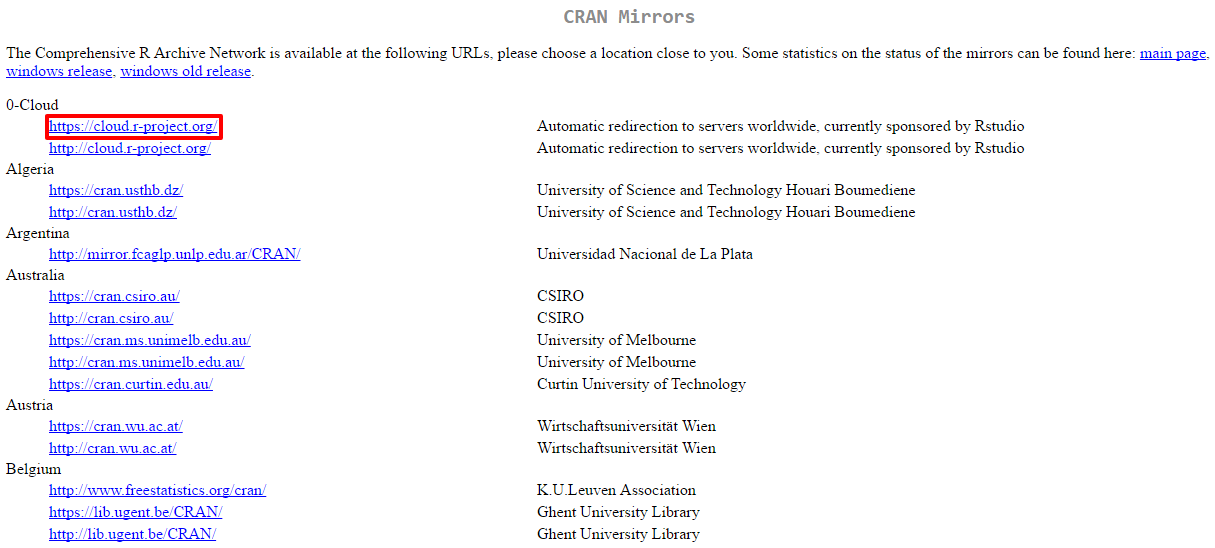
\includegraphics[width=1\linewidth]{figs/website_cran_2} 

}

\caption{Choosing the CRAN mirror}\label{fig:website-cran-2}
\end{figure}

The next step involves selecting your operating system. This is likely
to be \emph{Windows}. Due to the greater popularity of this platform,
from now on, we will focus on installing R in Windows. The instructions
for installing R in other operating systems can be easily found
\href{https://www.google.com.br/webhp?sourceid=chrome-instant\&ion=1\&espv=2\&ie=UTF-8\#q=installing+r\&*}{online}.
Regardless of the underlying platform, using R is about the same. There
are a few exceptions, especially when R interacts with the file system.
In the content of the book, special care was taken to choose functions
that work the same way in different operating systems. A few exceptions
are highlighted throughout the book. So, even if you are using Mac or
Linux, you can take full advantage of the material presented here .

\begin{figure}[!htbp]

{\centering 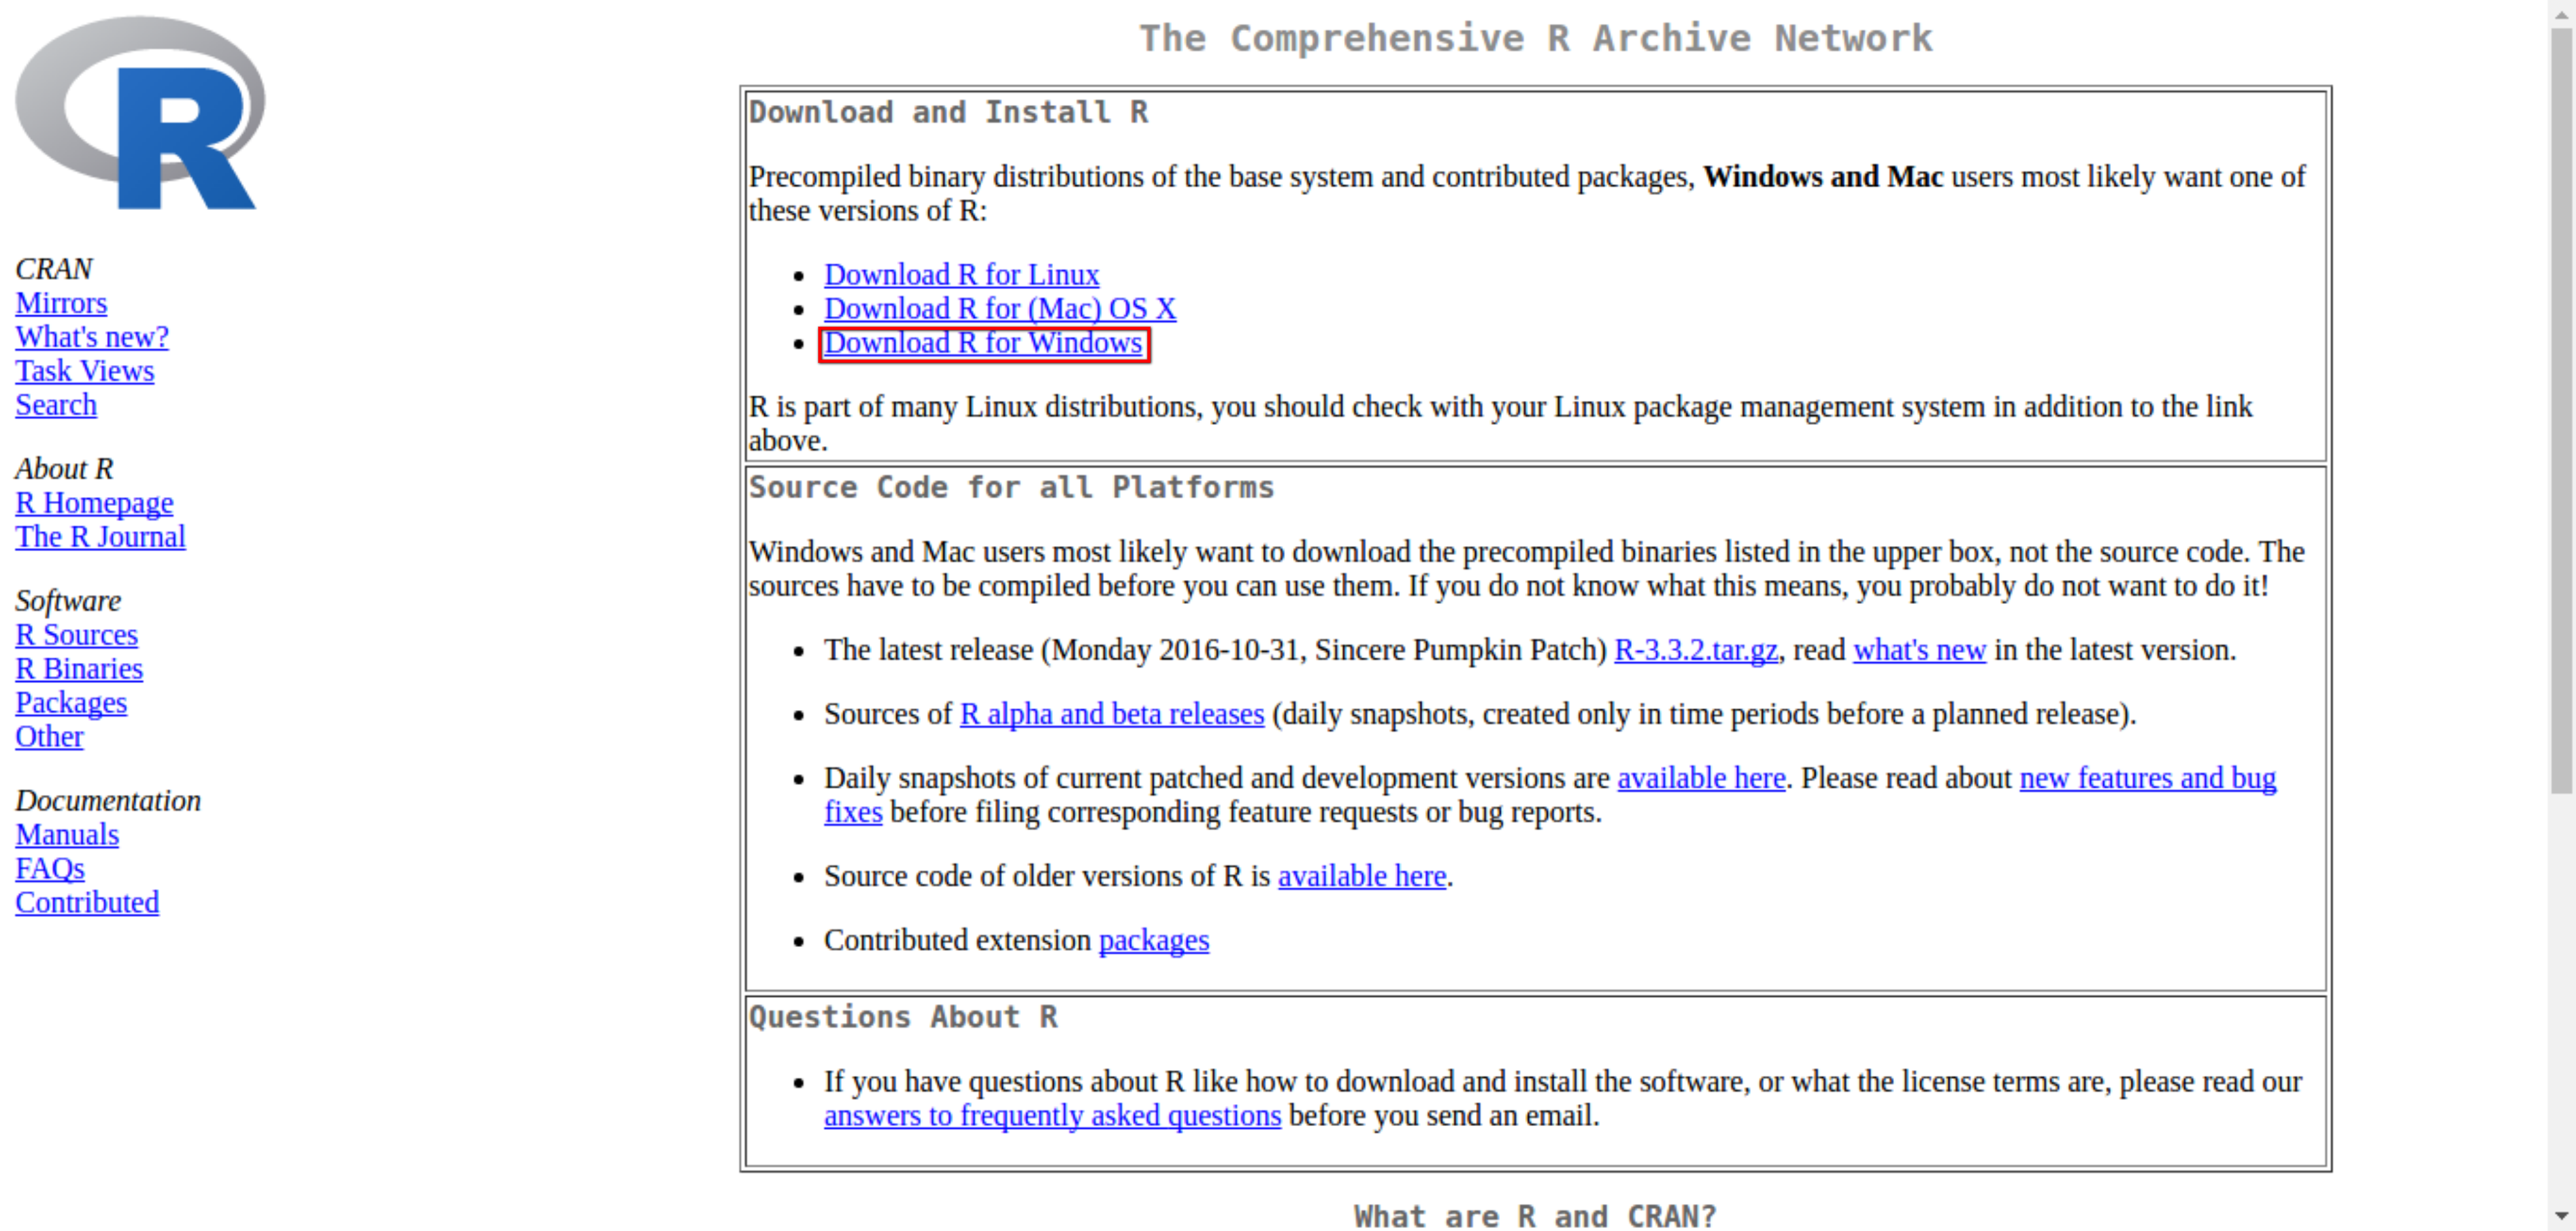
\includegraphics[width=1\linewidth]{figs/website_cran_3} 

}

\caption{Choosing the operating system}\label{fig:website-cran-3}
\end{figure}

After clicking the link \emph{Download R for Windows}, as in Figure
\ref{fig:website-cran-3}, the next screen will show the following
download options: \emph{base}, \emph{contrib}, \emph{old.contrib} and
\emph{RTools}. Among the \emph{download} options, the first
(\emph{base}), should be selected. It contains the basic installation of
R in \emph{Windows}. If the user is interested in creating and
distributing their own R packages, it is necessary to install
\emph{RTools}. For most users, however, this should not be the case, so
I suggest ignoring this program. The links to \emph{contrib} and
\emph{old.contrib} relate to files for the current and old releases of R
packages. You should not worry about it for now. We will discuss the use
of packages in the next chapter.

\begin{figure}[!htbp]

{\centering 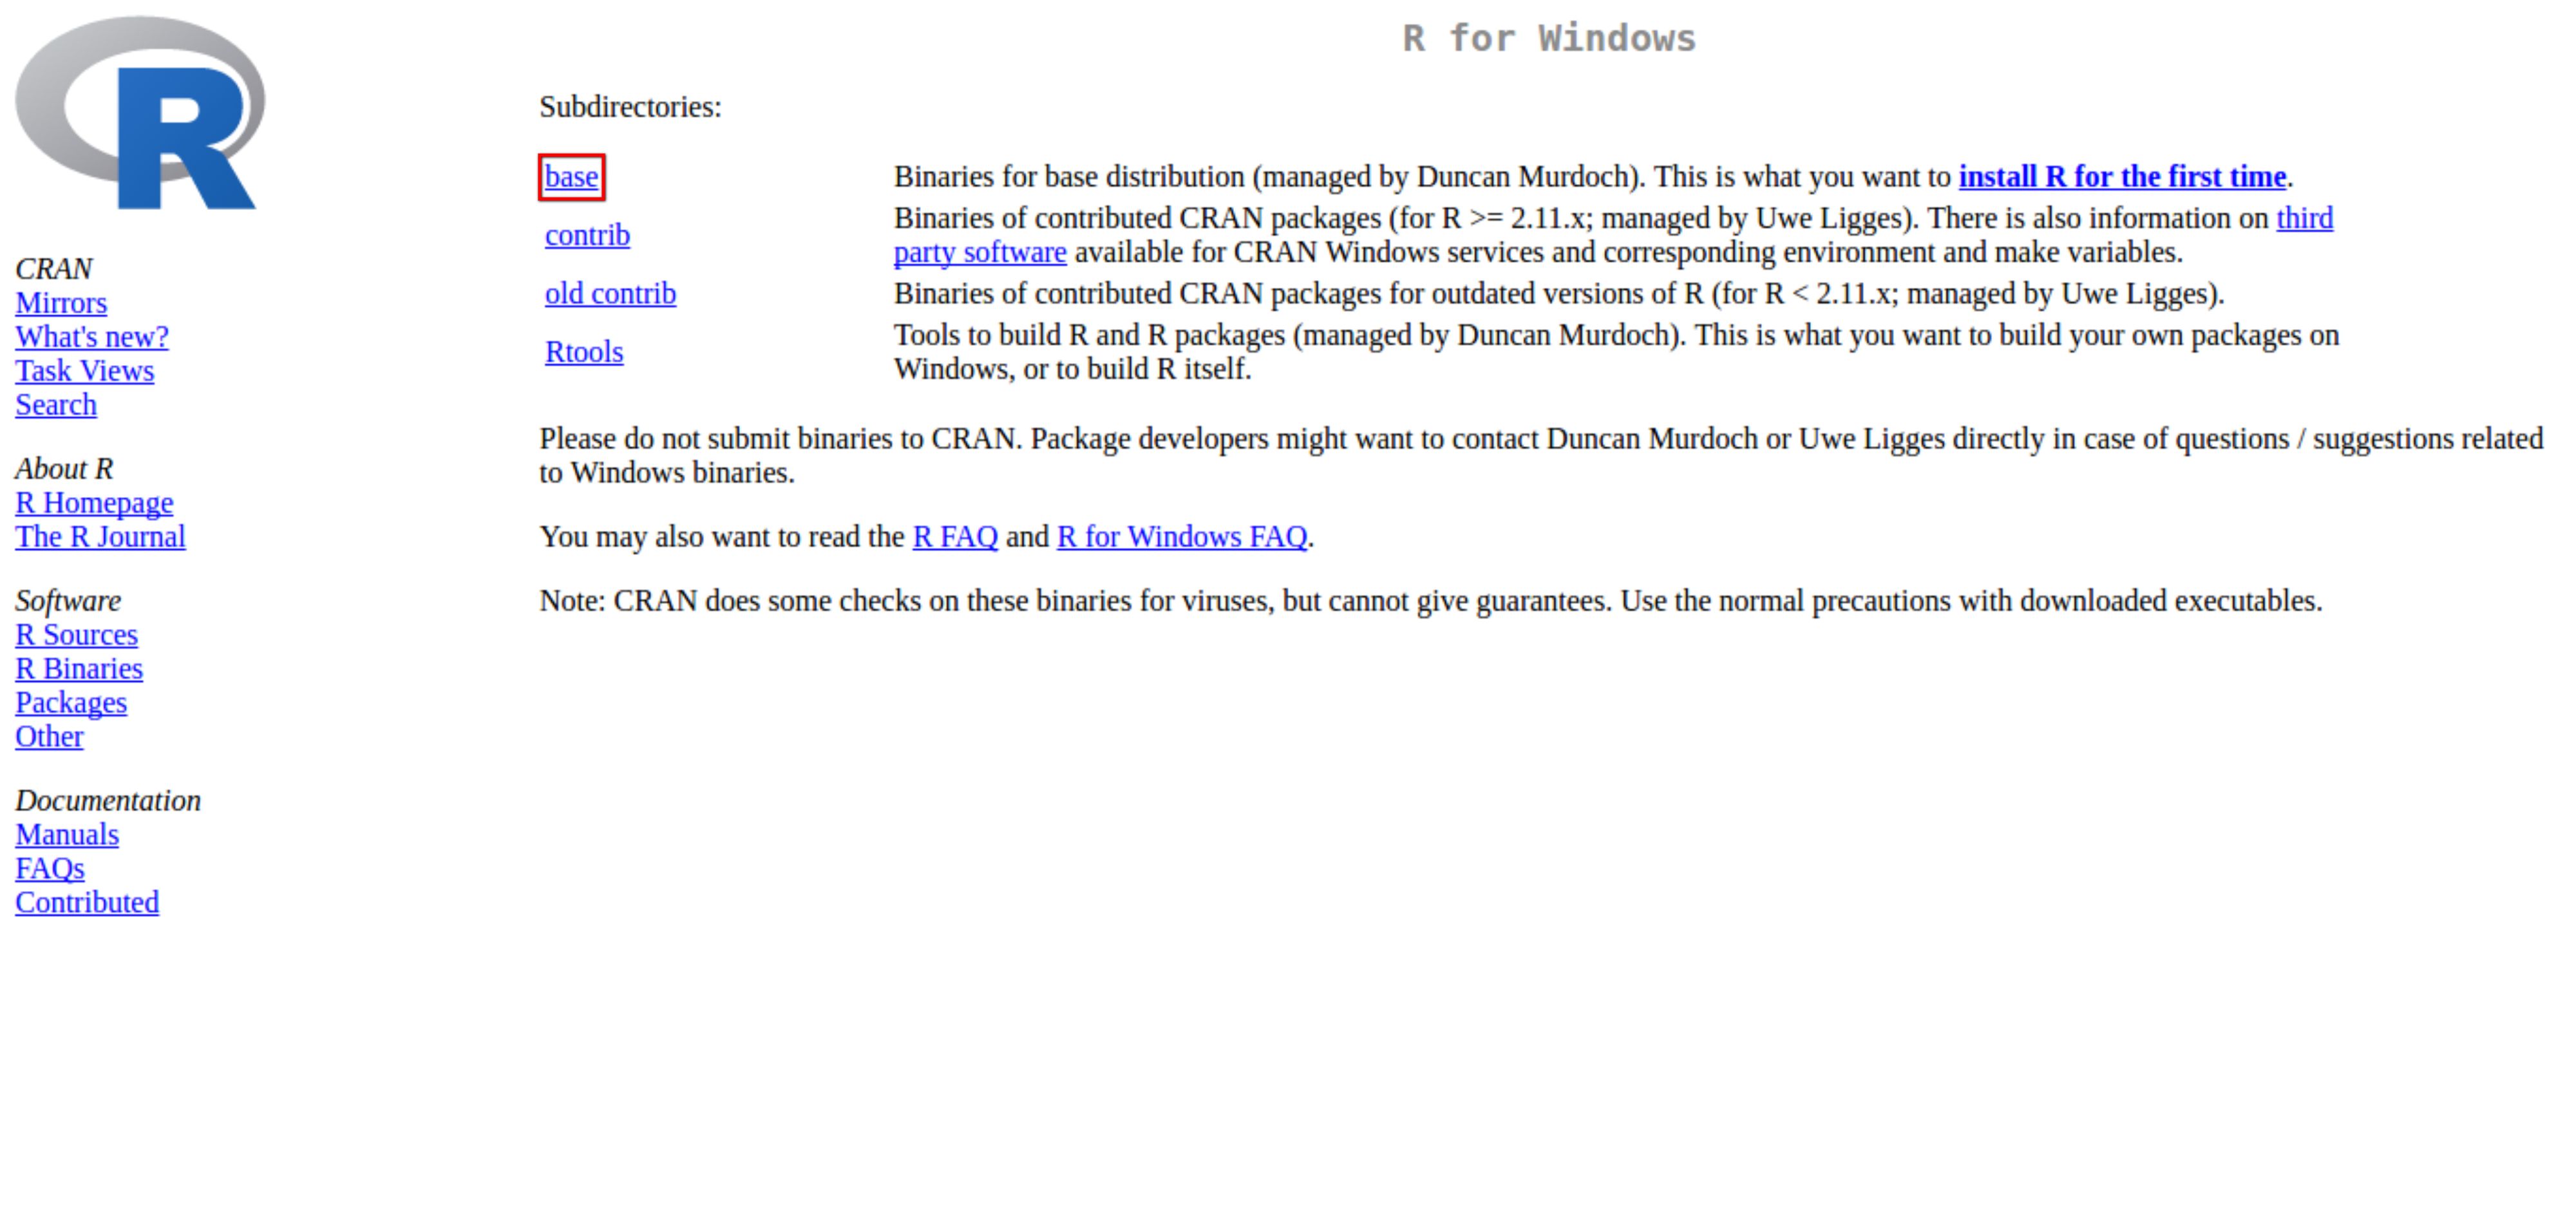
\includegraphics[width=1\linewidth]{figs/website_cran_4} 

}

\caption{Installation options}\label{fig:website-cran-4}
\end{figure}

After clicking the link \emph{base}, the next screen will show the link
to the \emph{download} of the R installation file (Figure
\ref{fig:website-cran-5}). After downloading the file, open it and
follow the steps in the installation screen. At this time, no special
configuration is required. I suggest keeping all the default choices and
simply hit \emph{accept} in the displayed dialogue screens. After the
installation of R, it is strongly recommended to install RStudio, which
will be addressed next .

\begin{figure}[!htbp]

{\centering 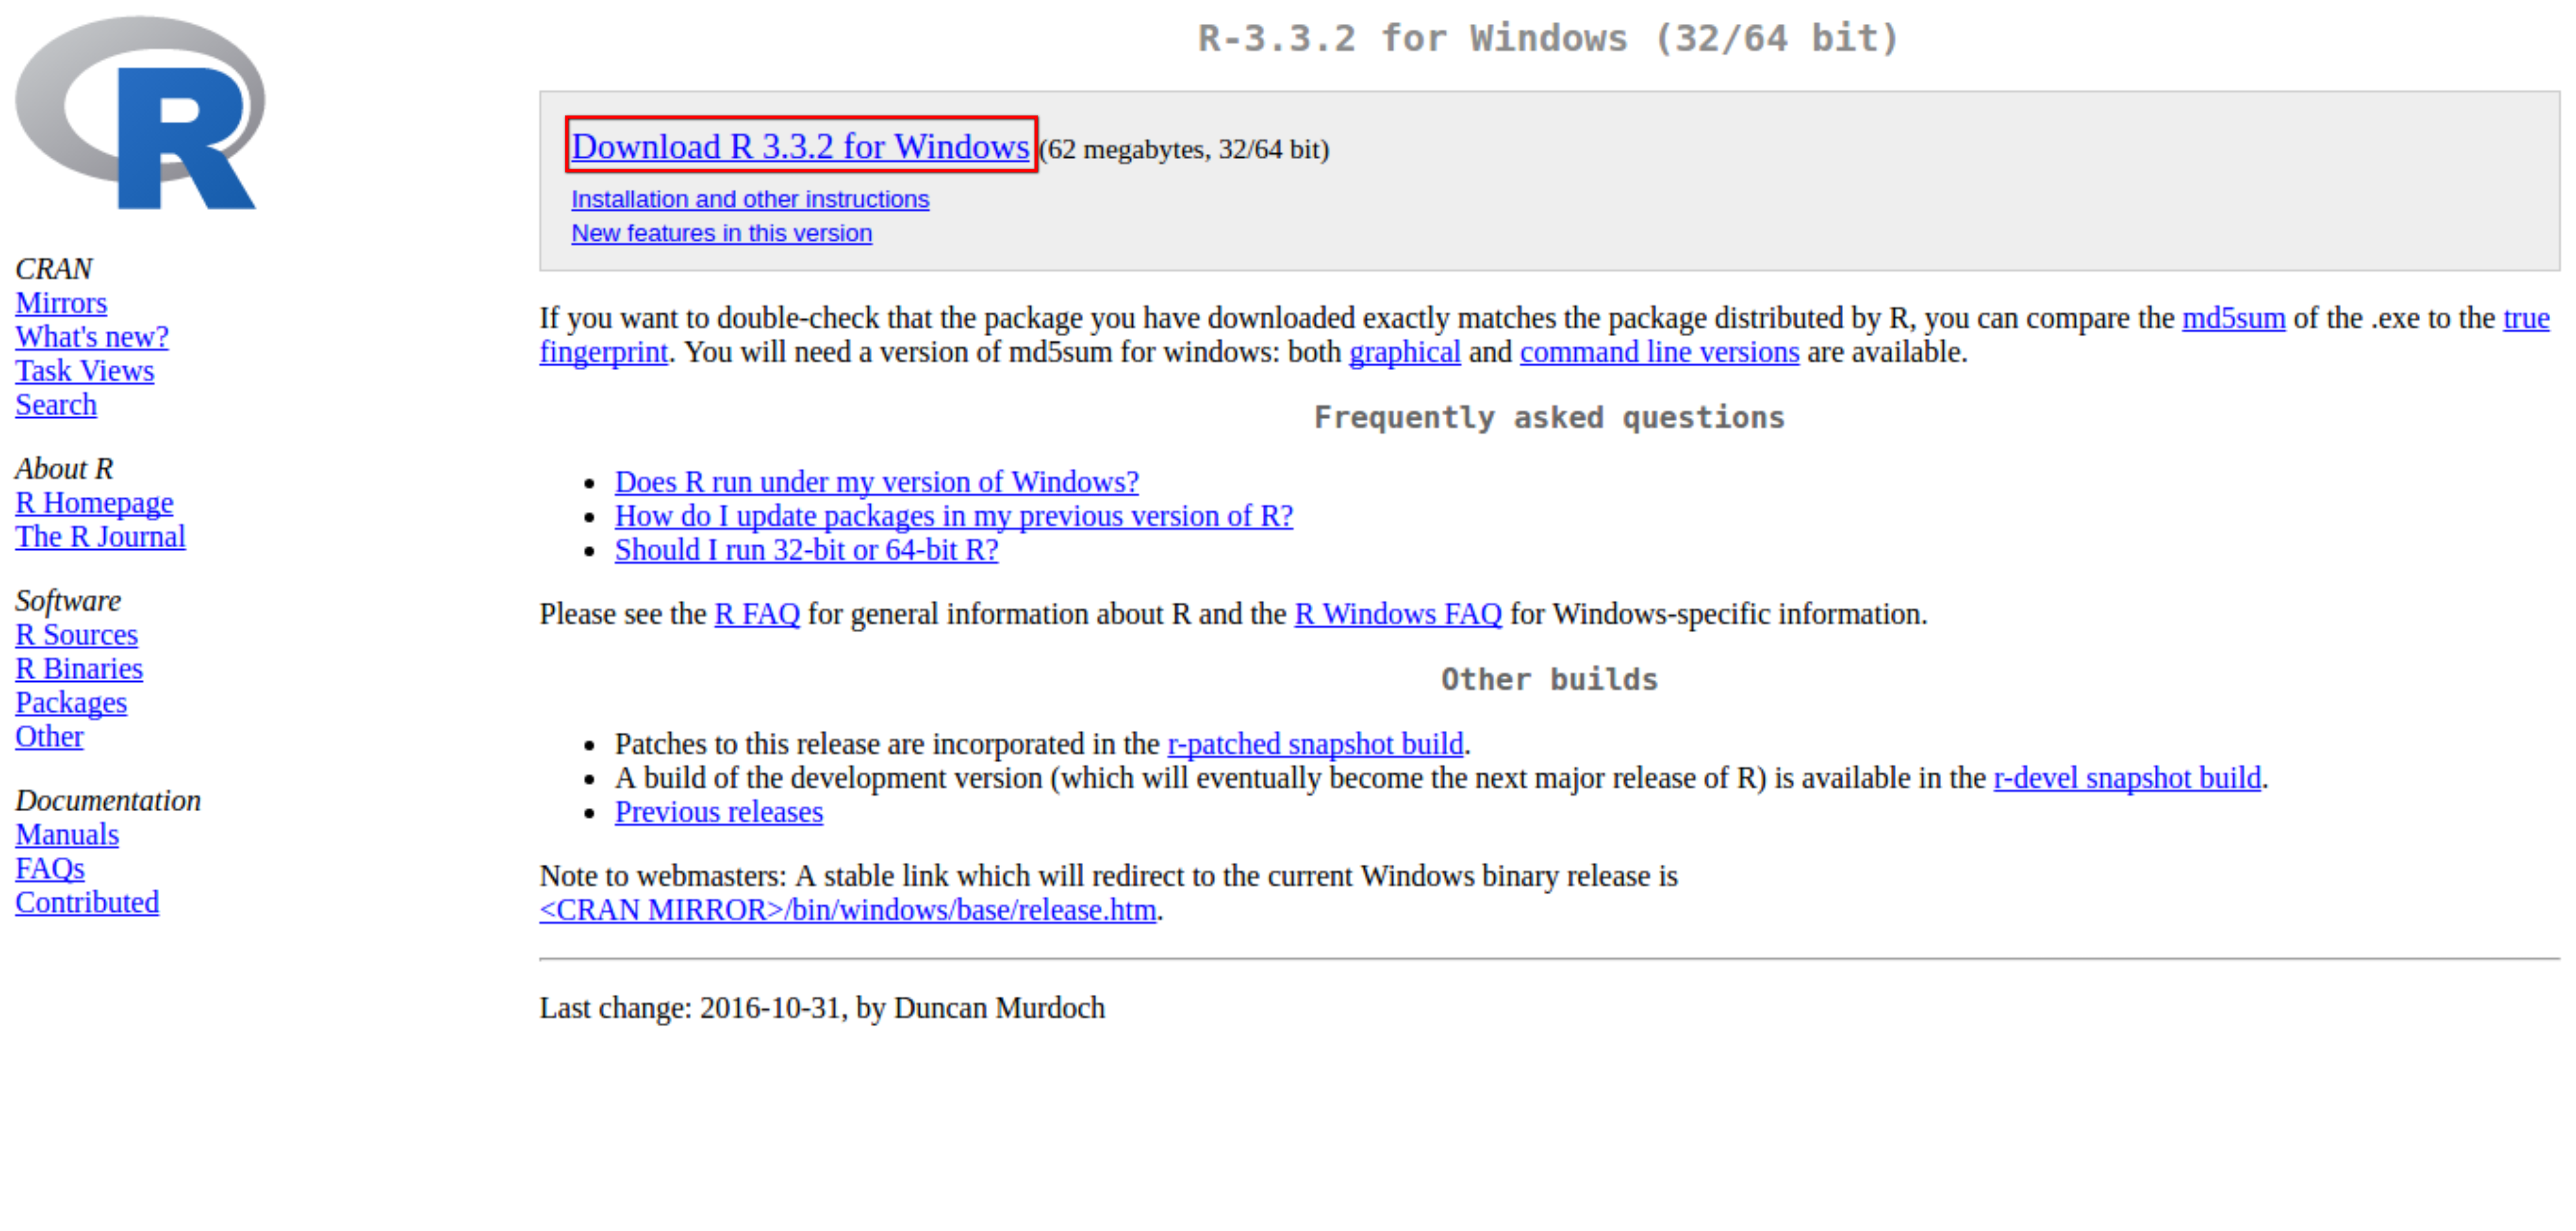
\includegraphics[width=1\linewidth]{figs/website_cran_5} 

}

\caption{Downloading R}\label{fig:website-cran-5}
\end{figure}

The base installation of R includes its own \emph{GUI} (graphical user
interface) that facilitates the use of the program. However, this native
interface has several limitations. RStudio is a software that
substitutes the original interface and makes the access to R more
practical and efficient. One way to understand this relationship is with
an analogy with cars. While R is the engine of the programming language,
RStudio is the body and instrument panel, which significantly improve
the user experience. Besides presenting a more attractive look, RStudio
also adds several features that make the life of a programmer easier,
allowing the creation of projects and packages, creation of dynamic
documents (\emph{Sweave/knitr}), among others. As an example, the book
you are reading was written in RStudio with package \texttt{bookdown}.
\index{RStudio} \index{bookdown}

The installation of RStudio is simpler than that of R. The files are
available in \href{https://www.rstudio.com/}{RStudio website}, provided
in the \href{https://sites.google.com/view/pafdr/home}{book site}. After
accessing the page, click \emph{Download RStudio} and then
\emph{Download RStudio Desktop}. After that, just select the
installation file relative to the operating system on which you will
work. This option is probably \emph{WINDOWS Vista 7/8/10}. Note that, as
well as R, RStudio is also available for alternative platforms.

I emphasize that using RStudio is not essential to develop programs in
R. Other interface software are available and can be used. However, in
my experience, RStudio is the interface that offers the widest range of
features for the language and is widely used, which justifies its
choice.

\section{Resources in the Web}\label{resources-in-the-web}

The R community is vivid and engaging. There are many authors, such as
myself, that constantly release material about R in their blogs and are
happy to discuss it. It includes package announcements, posts about data
analysis in real life, curiosities, rants and tutorials.
\href{https://www.r-bloggers.com/}{R-Bloggers} is a website that
aggregates these blogs in a single place, making it easier for anyone to
access and participate. I strongly recommend to sign up for the
R-Bloggers feed in \href{https://feeds.feedburner.com/RBloggers}{RSS},
\href{https://www.facebook.com/rbloggers/?fref=ts}{Facebook} or
\href{https://twitter.com/Rbloggers}{Twitter}. Not only you'll be
informed of what is happening in the R community, but also learn a lot
by reading other people code and articles.

Learning and using R can be a social experience. Several conferences and
user-groups are available in many countries. You can find the complete
list in this
\href{https://jumpingrivers.github.io/meetingsR/index.html}{link}. I
also suggest looking for local groups in Facebook. These may not be
registered in the previous link.

\section{Structure and Organization}\label{structure-and-organization}

This book presents a practical approach to the use of R in finance,
accompanied by R code, which will show and illustrate the functionality
of the program. To get the most out of this book, I suggest you first
seek to understand the code shown, and only then, try using it on your
own computer.

Learning to program in a new language is like learning a foreign spoken
language: the use in day-to-day problems is imperative to create
fluency. All the code and data used in this book is available in the
\href{https://sites.google.com/view/pafdr/home}{book webpage}. I suggest
you test the code on your computer and \emph{play} with it, modifying
the examples and checking the effect of changes in the outputs. Whenever
you have a computational problem, try using R for solving it. You'll
stumble and make mistakes at first. But I guarantee that, soon enough,
you'll be able to write complex data tasks effortlessly.

Throughout the book, every demonstration of code will have two parts:
the R code and its output. The output is nothing more than the result of
the commands in the program screen. All inputs and outputs code will be
marked in the text with a special format. See the following example:

\begin{Shaded}
\begin{Highlighting}[]
\CommentTok{# create a list}
\NormalTok{x <-}\StringTok{ }\KeywordTok{list}\NormalTok{(}\StringTok{'abc'}\NormalTok{, }\DecValTok{1}\OperatorTok{:}\DecValTok{5}\NormalTok{, }\StringTok{'dec'}\NormalTok{)}

\CommentTok{# print list}
\KeywordTok{print}\NormalTok{(x)}
\end{Highlighting}
\end{Shaded}

\begin{verbatim}
## [[1]]
## [1] "abc"
## 
## [[2]]
## [1] 1 2 3 4 5
## 
## [[3]]
## [1] "dec"
\end{verbatim}

For the previous chunk of code, lines
\texttt{x\ \textless{}-\ list(\textquotesingle{}abc\textquotesingle{},\ 1:5,\ \textquotesingle{}dec\textquotesingle{})}
and \texttt{print(x)} are actual commands given to R. The program output
is the on-screen presentation of the contents of object \texttt{x} with
the predecessor symbol \texttt{\#\#}. This symbol is used for any code
output. Notice also that inline comments are set with the symbol
\texttt{\#}. Anything in the right side of \texttt{\#} is not evaluated
by R. These comments serve as written notes about the code.

Code can also be spatially organized using new lines. This is a common
procedure around arguments of functions. The next chunk of code is
equivalent to the previous, and will run the exact same way. Notice how
we used a new line to vertically align the arguments of function
\texttt{list}. You'll soon see that, throughout the book, this type of
vertical alignment is constantly used.

\begin{Shaded}
\begin{Highlighting}[]
\CommentTok{# create a list}
\NormalTok{x <-}\StringTok{ }\KeywordTok{list}\NormalTok{(}\StringTok{'abc'}\NormalTok{, }
          \DecValTok{1}\OperatorTok{:}\DecValTok{5}\NormalTok{, }
          \StringTok{'dec'}\NormalTok{)}

\CommentTok{# print list}
\KeywordTok{print}\NormalTok{(x)}
\end{Highlighting}
\end{Shaded}

\begin{verbatim}
## [[1]]
## [1] "abc"
## 
## [[2]]
## [1] 1 2 3 4 5
## 
## [[3]]
## [1] "dec"
\end{verbatim}

The code also follows a well-defined structure. One decision in writing
computer code is how to name objects and how to structure it. It is
recommended to follow a clear pattern, so it is easy to maintain over
time and be used and understood by others. For this book, a mixture of
the author's personal choices with the coding style suggested by Google
(link on the \href{https://sites.google.com/view/pafdr/home}{book
website}) was used. The reader, however, may choose the structure he
finds more efficient and aesthetically pleasing. Like many things in
life, this is a choice.

\hypertarget{basicoperations}{\chapter{Basic Operations in
R}\label{basicoperations}}

Before you start developing your code, you need to understand how to
work with R and RStudio. This includes work patterns, language
components, basic commands and RStudio shortcuts. Understanding the
software and how to take advantage of the platform is essential for the
development of data-based research scripts. This is the main chapter for
those who are not familiar with R or other programming languages.

In this section, we will go through the initial steps from the point of
view of someone who has never worked with R and possibly never had
contact with another programming language. Those already familiar with
the program will not find novel information here and therefore, I
suggest you skip to the next section. It is recommended, however, that
you at least check the topics discussed here so that you can confirm
your knowledge about the features of the program.

\section{Working With R}\label{working-with-r}

The greatest difficulty a new user experiences when starting to develop
routines in R is the format of work. Our interaction with computers has
been simplified over the years and we are currently comfortable with the
\emph{point\&click} format. That is, if you want to perform some
operation on the computer, just point the \emph{mouse} to the specific
location on the screen and click the button that performs the operation.
Visual cues and a series of steps in this direction allows the execution
of complex tasks. But, be aware that this form of interaction is just
one layer above what actually happens on the computer. Behind all these
\emph{clicks}, there is a command being executed. Any common task such
as opening a \emph{pdf} file, a spreadsheet document, directing a
\emph{browser} to a web page has an underlying call to a command. This
command was created by the program developer to run within your
operating system.

While this visual and motor interaction format has its benefits in
facilitating and popularizing the use of computers, it is not flexible
and effective when working with computational procedures. By knowing the
commands available to the user, it is possible to create a file
containing several instructions in sequence and, in the future, simply
request that the computer \textbf{execute} this file using the recorded
procedures. There is no need to do a ``scripted'' point\&click
operation. You need to spend some time creating the program but, in the
future, it will always execute the recorded procedure in the same way.
In the medium and long term, there is a significant gain in productivity
between the use of a \emph{script} (sequence of commands) and a
\emph{point\&click} type of interface. Going further, the risk of human
error in executing the procedure is almost nil because the commands and
their sequence are recorded in the text file and will always be executed
in the same way. This is one of the main reasons why programming
languages are popular in science. All steps of data based research can
be replicated.

In the use of R, the ideal format of work is to merge the use of the
mouse with commands. R and RStudio have some functionality with the
\emph{mouse}, but their capacity is optimized when we perform operations
using code. When a group of commands is performed in a smart way, we
have an R script that should preferably produce something important to
us at the end of its execution. In Finance, this can be the updated
value of an investment, the calculation of the risk of a portfolio, the
historical performance of an investment strategy, the result of an
academic research, among many other possibilities.

Like other software, R allows us to import data and export files. We can
use code to import a dataset stored in a local file (or the web), do an
analysis of this data and save the results to later import it into a
technical report. In fact, we can use RStudio to write a dynamic report,
where code and content are integrated, using \emph{knitr} and
\emph{Sweave} \citep{leisch2002sweave}. For example, the book you're
reading was written using \emph{knitr} and the \texttt{bookdown} package
\citep{xie2016bookdown}. The book is compiled with the execution of the
R codes and their outputs are recorded in the scope of the text. All
figures and data tasks in the book can be updated with the execution of
a simple command. Needless to say that by using the capabilities of R
and RStudio, you will work smarter and faster. \index{bookdown}
\index{knitr}

\section{Objects in R}\label{objects-in-r}

\textbf{In R, everything is an object, and each type of object has its
properties}. For example, the daily market closing prices of a stock can
be represented as a numerical vector, where each element is a price
recorded at the end of a trading day. Dates and times related to these
prices can be represented as text (\emph{string}) or one of the
\texttt{datetime} classes. Finally, we can represent the price data and
the dates together by storing them in a single object of type
\emph{dataframe}, which is nothing more than a table with rows and
columns. These objects are part of the R ecosystem, and it is through
their manipulation that we take full advantage of the software.

While we represent data as objects in R, a special type is a
\texttt{function}, which stores a pre-established procedure that is
available to the user. R has an extremely large number of functions,
which enable the user to perform a wide range of operations. For
example, the basic commands of R, available in the package
\texttt{base}, adds up to a total of 1217 functions. Each function has
its own name and a programmer can write their own functions. For
example, the \texttt{mean} function is a procedure that calculates the
average values of a vector. If we wanted to calculate the average value
of the sequence \texttt{1,\ 2,\ 3,\ 4,\ 5}, simply insert the following
command in the \emph{prompt} (left bottom of RStudio) and press
\emph{enter}: \index{base!mean} \index{functions}

\begin{Shaded}
\begin{Highlighting}[]
\KeywordTok{mean}\NormalTok{(}\DecValTok{1}\OperatorTok{:}\DecValTok{5}\NormalTok{, }\DataTypeTok{na.rm =} \OtherTok{TRUE}\NormalTok{)}
\end{Highlighting}
\end{Shaded}

\begin{verbatim}
## [1] 3
\end{verbatim}

The \emph{:} symbol used above creates a sequence starting at 1 and
ending at 5 (more details about this operator in a later section). Note
that the \texttt{mean} function is used with start and end parentheses.
These parentheses serve to highlight the entries (\emph{inputs}), that
is, the information sent to the function to produce something. Note that
each entry is separated by a comma, as in
\texttt{MyFct(input1,\ input2,\ input3,\ ...)}. We also set option
\texttt{na.rm\ =\ TRUE}. This is a specific directive for the
\texttt{mean} function to ignore elements of type \texttt{NA} (\emph{not
available}), if they exist. This specific type of object will also be
discussed in a future chapter.

Functions are at the heart of R and we will dedicate a large part of
this book to them. You can use the available functions or write your
own. You can also publish your functions and let other people use your
code. In a later chapter, we will learn how to use functions to do data
analysis in an efficient way.

\section{International and Local
Formats}\label{international-and-local-formats}

Before beginning to explain the use of R and RStudio, it is important to
highlight some rules of formatting numbers, Latin characters and date
formats.

\begin{itemize}
\item
  \textbf{decimal:} Following an international notation, the decimal
  point in R is defined by the period symbol (.), as in \texttt{2.5} and
  not comma, as in \texttt{2,5}. In some countries, this might not be
  the case. This difference can create a lot of confusion and errors at
  the beginning. Some software, such as Microsoft Excel, does the
  conversion automatically when the data is imported. This, however, is
  generally an exception. As a general rule of using R, only use commas
  to separate the inputs of a function. Under no circumstances should
  the comma symbol be used as the decimal point separator. Always give
  priority to the international format because it will be compatible
  with the vast majority of data. Other researchers may experience some
  difficulty in understanding your code if you use your local notation
  for the decimal. \index{decimal}
\item
  \textbf{Latin characters:} Due to its international standard, R has
  problems understanding Latin characters, such as the cedilla and
  accents. If you can avoid it, do not use these characters in the names
  of your variables or files. In character objects (text), you can use
  them without problems as long as the encoding is correctly specified
  (e.g.~UTF-8, Latin1). Given that, it is recommended that the R code be
  written in the English language. This automatically eliminates the use
  of Latin characters and facilitates the usability of the code by
  people outside of your country. \index{latin characters} \index{UTF-8}
  \index{Latin1}
\item
  \textbf{date format:} Dates in R are formatted according to the
  \texttt{YYYY-MM-DD} pattern, where \texttt{YYYY} is the year in four
  numbers, \texttt{MM} is the month and \texttt{DD} is the day. An
  example is 2017-05-03. This may not be the case in your country. When
  importing local datasets, make sure that the dates are in this format
  or do a conversion. Again, while you can work with your local format
  of dates in R, it is best advised to use the international notation.
  The conversion between one format and another is quite easy and will
  be presented in a future chapter. \index{dates}
\end{itemize}

If you want to learn more about your local format in R, use the
following command by typing it in the prompt and pressing enter:

\begin{Shaded}
\begin{Highlighting}[]
\KeywordTok{Sys.localeconv}\NormalTok{()}
\end{Highlighting}
\end{Shaded}

\begin{verbatim}
##     decimal_point     thousands_sep          grouping 
##               "."                ""                "" 
##   int_curr_symbol   currency_symbol mon_decimal_point 
##             "BRL"              "R$"               "," 
## mon_thousands_sep      mon_grouping     positive_sign 
##               "."            "\003"                "" 
##     negative_sign   int_frac_digits       frac_digits 
##               "-"               "2"               "2" 
##     p_cs_precedes    p_sep_by_space     n_cs_precedes 
##               "1"               "1"               "1" 
##    n_sep_by_space       p_sign_posn       n_sign_posn 
##               "1"               "3"               "3"
\end{verbatim}

The output of \texttt{Sys.localeconv()} shows how R interprets decimal
points and the thousands separator, among other things. As you can see
from the previous output, this book was compiled using the Brazilian
notation for currency but uses the dot point for decimals. As mentioned
before, it is good policy to follow international notation, especially
for the decimal point. If necessary, you can change your local format to
the US/international notation using the following command.

\begin{Shaded}
\begin{Highlighting}[]
\KeywordTok{Sys.setlocale}\NormalTok{(}\StringTok{"LC_ALL"}\NormalTok{, }\StringTok{"English"}\NormalTok{)}
\end{Highlighting}
\end{Shaded}

A note, however, is that you'll need to run this command every time that
R starts or incorporate it in the initialization of the software.

\section{Types of Files in R}\label{types-of-files-in-r}

Like any other programming platform, R has a file ecosystem and each
type of file has a different purpose. In the vast majority of cases,
however, the work will focus mostly on two types: \emph{.R} and
\emph{.RData} files. Next, I provide a description of various file
extensions. The items in the list are ordered by importance. Note that
we omit graphic files such as \emph{.png}, \emph{.jpg}, \emph{.gif} and
data storage files (\emph{.csv}, \emph{.xlsx}, ..) among others, as they
are not exclusive to R. \index{file types!.R} \index{file types!.RData}
\index{file types!.Rmd}

\begin{itemize}
\item
  \textbf{Files with the extension \emph{.R }}: text files containing
  several instructions for R. These are the files that will contain the
  sequence of commands that configures the main script and subroutines
  of the data research. Examples: My-Research.R, My\_Functions.R.
\item
  \textbf{Files with extension \emph{.RData}}: files that store data in
  R native format. These files are used to save (write) objects created
  in different sessions. For example, you can use a \emph{.RData} file
  to save a table after processing and cleaning up the raw database.
  This file can be later loaded for a subsequent analysis. Examples:
  My\_data.RData, Research\_Results.RData.
\item
  \textbf{Files with extension \emph{.Rmd}, \emph{.md} and \emph{.Rnw}}:
  represent files used for editing dynamic documents related to the
  \emph{Rmarkdown} and \emph{markdown} formats. The use of these files
  allows the creation of documents where text and code output are
  integrated. This is an advanced topic and will not be covered in this
  book. For those interested, I suggest reading \citet{baumer2014r} and
  a tutorial at this
  \href{http://rmarkdown.rstudio.com/index.html}{link}. Example:
  My\_Report.Rmd. \index{Rmarkdown} \index{markdown}
\item
  \textbf{Files with extension \emph{.Rproj}}: contain files for editing
  projects in RStudio, such as a new package, a \emph{shiny} application
  or a book. This is also an advanced topic and will not be dealt with
  here. While you can use the functionalities of RStudio projects to
  write R scripts, it is not a necessity. For those interested in
  learning more about this functionality, I suggest the
  \href{https://support.rstudio.com/hc/en-us/articles/200526207-Using-Projects}{RStudio
  manual}. Example: MyProject.Rproj. \index{RStudio projects}
\end{itemize}

\section{Explaining the RStudio
Screen}\label{explaining-the-rstudio-screen}

After installing the two programs, R and RStudio, open RStudio by double
clicking its icon. It should be noted that R also has an interface
program and this often causes confusion. You should find the correct
shortcut for RStudio by going through your software folders. In Windows,
you can search for RStudio using the \emph{Start} button.
\index{RStudio}

After opening RStudio, the resulting window should look like Figure
\ref{fig:RStudio1}.

\begin{figure}[!htbp]

{\centering 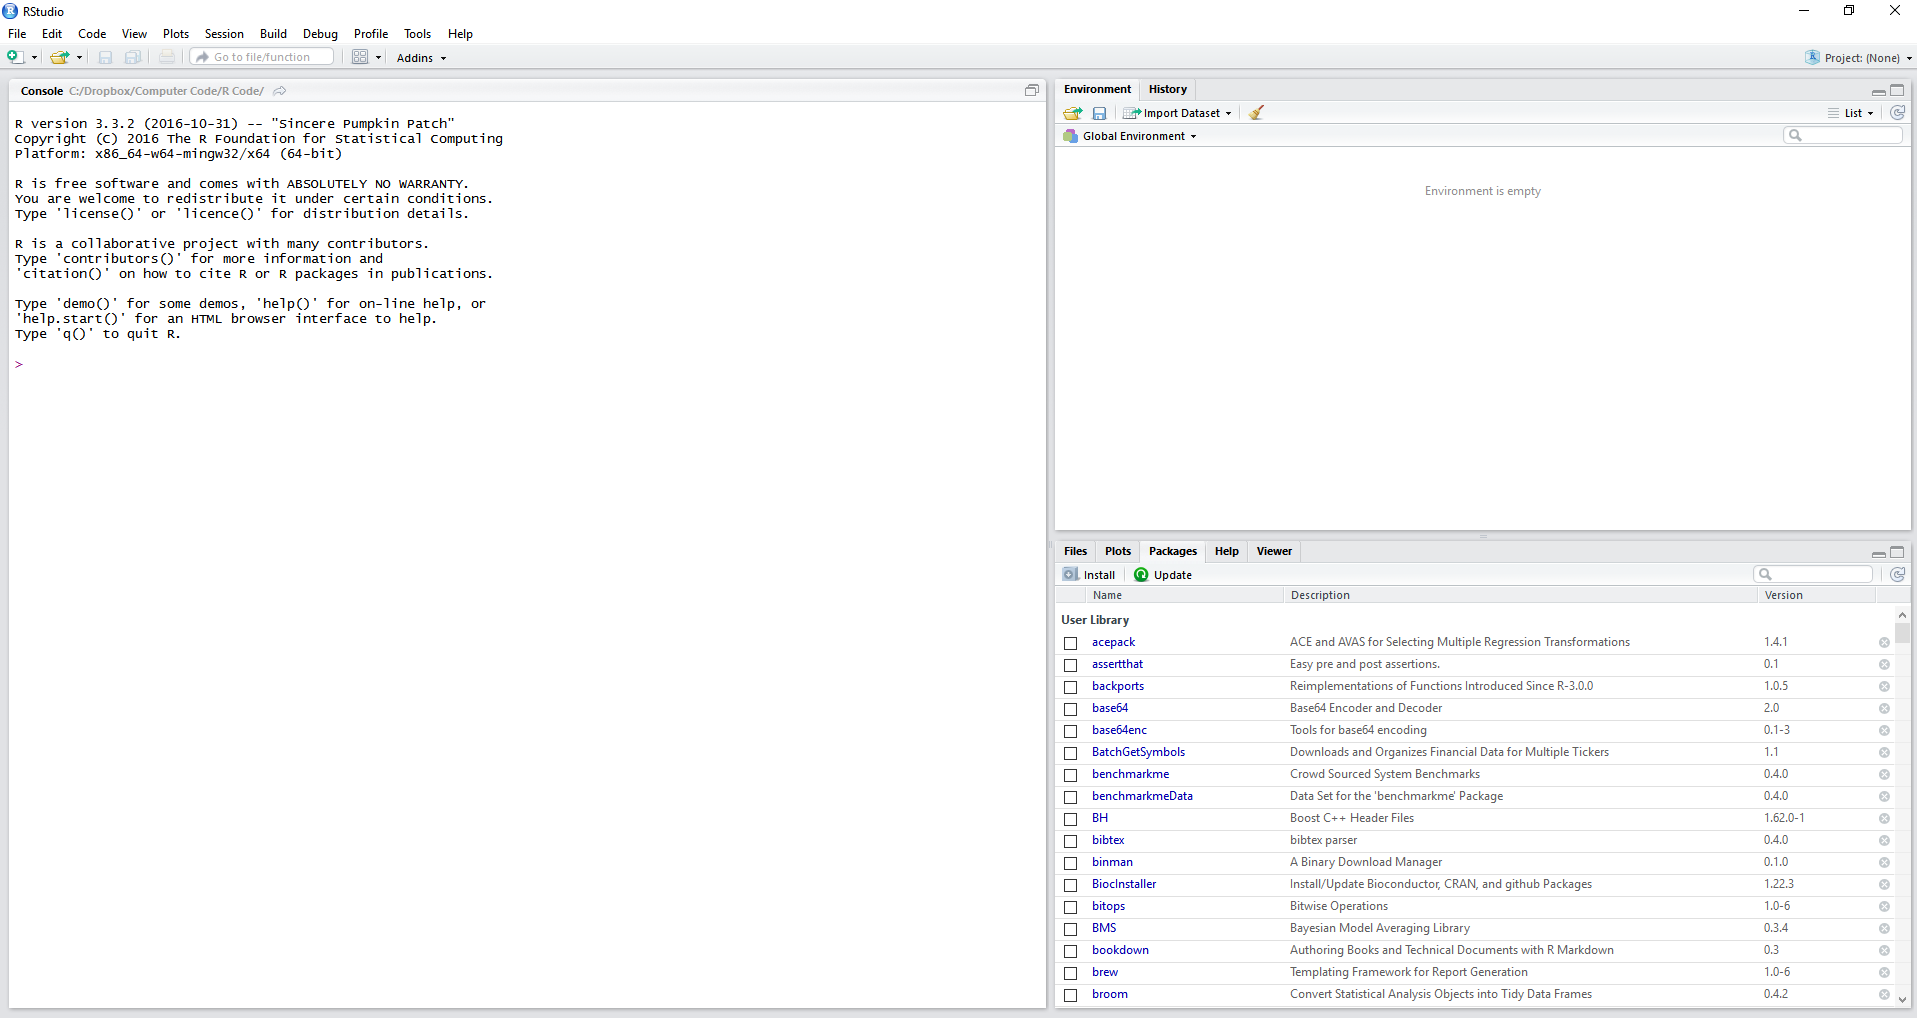
\includegraphics[width=1\linewidth]{figs/RStudio1} 

}

\caption{The RStudio screen}\label{fig:RStudio1}
\end{figure}

Note that RStudio automatically detected the installation of R and
initialized your screen on the left side.

If you do not see something like this on the screen of RStudio:

\begin{verbatim}
R version 3.3.3 (2017-03-06) -- "Another Canoe"
Copyright (C) 2017 The R Foundation for Statistical Computing
Platform: x86_64-w64-mingw32/x64 (64-bit)

R is free software and comes with ABSOLUTELY NO WARRANTY.
You are welcome to redistribute it under certain conditions.
Type 'license()' or 'licence()' for distribution details.

R is a collaborative project with many contributors.
Type 'contributors()' for more information and
'citation()' on how to cite R or R packages in publications.

Type 'demo()' for some demos, 'help()' for on-line help, or
'help.start()' for an HTML browser interface to help.
Type 'q()' to quit R.
\end{verbatim}

then R was not installed correctly. Repeat the installation steps in the
previous chapter and confirm the startup message on the lower left side
of RStudio.

As a first exercise, click \emph{file}, \emph{New File}, and \emph{R
Script}. A text editor should appear on the left side of the screen. It
is there that we will enter our commands, which are executed from top to
bottom, in the same direction that we normally read text. A side note,
all \emph{.R} files created in RStudio are just text files and can be
edited in other editors as well. It is not uncommon for experienced
programmers to use a specific software to write code and another to run
it. The resulting screen should look like the following:

\begin{figure}[!htbp]

{\centering 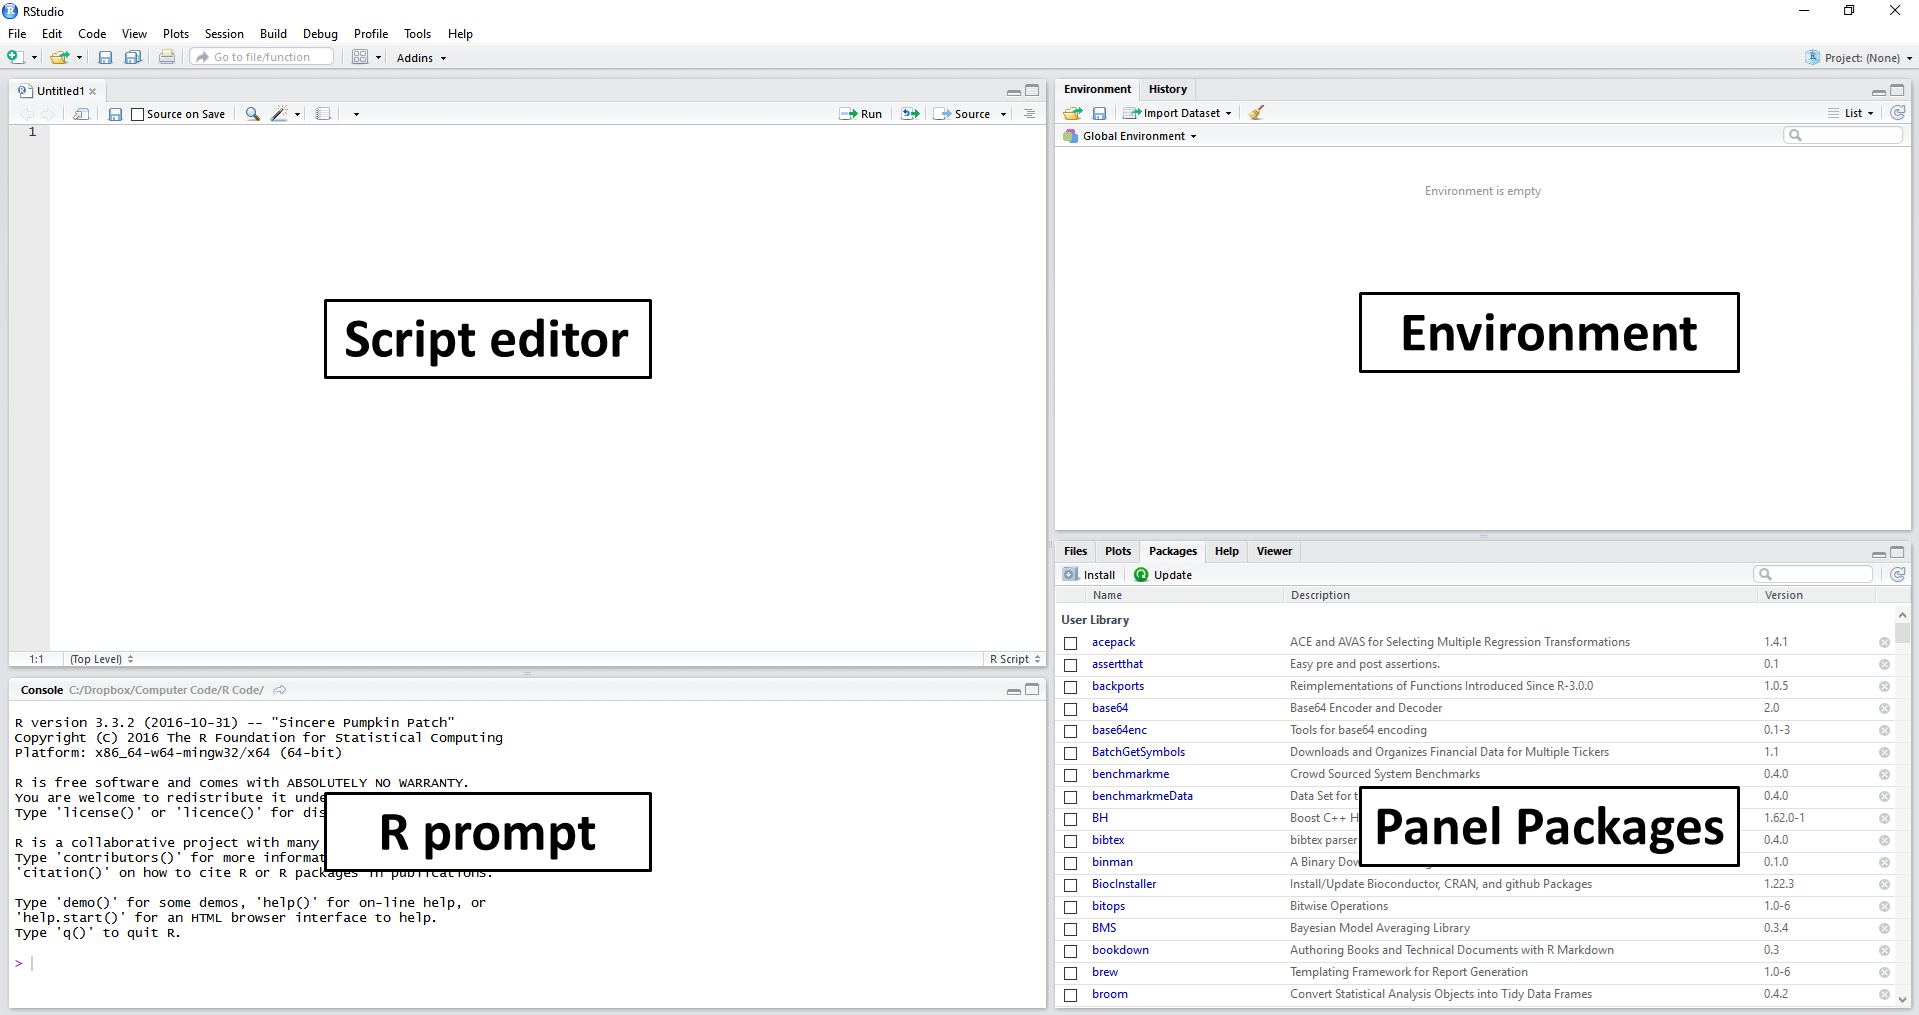
\includegraphics[width=1\linewidth]{figs/RStudio2} 

}

\caption{Explaining the RStudio screen}\label{fig:RStudio2}
\end{figure}

The main items/panels of the RStudio screen in Figure \ref{fig:RStudio2}
are:

\begin{itemize}
\item
  \textbf{Script Editor:} located on the left side and above the screen.
  This panel is used to write scripts and functions;
  \index{script editor}
\item
  \textbf{R prompt:} located on the left side and below the script
  editor. It displays the \emph{prompt} of R, which can also be used to
  give commands to R. The main function of the prompt is to test code
  and display the results of the commands entered in the script editor;
  \index{prompt}
\item
  \textbf{Environment:} located on the top-right of the screen. Shows
  all objects, including variables and functions currently available to
  the user. Also note a \emph{History} panel, which shows the history of
  the commands previously executed by the user; \index{environment}
\item
  \textbf{Panel Packages:} shows the packages installed and loaded by R.
  Here you have four tabs: \emph{Files}, to load and view system files;
  \emph{Plots}, to view pictures; \emph{Help} to access the help system
  and \emph{Viewer} to display dynamic and interactive results, such as
  a web page. \index{RStudio panels}
\end{itemize}

As an introductory exercise, let's initialize two objects in R. Inside
the prompt (lower left side), insert the following commands and press
\emph{enter} at the end of each. The \texttt{\textless{}-} symbol is
nothing more than the result of joining \texttt{\textless{}} (less than)
with the \texttt{-} (minus sign). The \texttt{\textquotesingle{}} symbol
represents a single quotation mark and, in the computer keyboard, it is
found under the escape (\emph{esc}) key.

\begin{Shaded}
\begin{Highlighting}[]
\CommentTok{# set x}
\NormalTok{x <-}\StringTok{ }\DecValTok{1}

\CommentTok{# set y}
\NormalTok{y <-}\StringTok{ 'My humble text'}
\end{Highlighting}
\end{Shaded}

If done correctly, notice that two objects appeared in the
\emph{environment} panel, one called \texttt{x} with a value of 1, and
another called \texttt{y} with the text content
\texttt{"My\ humble\ text"}. Notice how we used specific symbols to
define objects \texttt{x} and \texttt{y}. The use of double quotes
(\texttt{"\ "}) or single quotes
(\texttt{\textquotesingle{}\ \textquotesingle{}}) defines objects of the
class \texttt{character}. Numbers are defined by the value itself. As
will be discussed later, each object in R has a class and each class has
a different behaviour. After sending the previous commands to R, the
\emph{history tab} has been updated.

Now, let's show the values of \texttt{x} on the screen. To do this, type
the following command:

\begin{Shaded}
\begin{Highlighting}[]
\CommentTok{# print contents of x}
\KeywordTok{print}\NormalTok{(x)}
\end{Highlighting}
\end{Shaded}

\begin{verbatim}
## [1] 1
\end{verbatim}

The \texttt{print} function is one of the main functions for displaying
values in the \emph{prompt} of R. The text displayed as \texttt{{[}1{]}}
indicates the index of the first line number. To verify this, enter the
following command, which will show a lengthy sequence of numbers on the
screen: \index{base!print}

\begin{Shaded}
\begin{Highlighting}[]
\CommentTok{# print a sequence}
\KeywordTok{print}\NormalTok{(}\DecValTok{50}\OperatorTok{:}\DecValTok{100}\NormalTok{)}
\end{Highlighting}
\end{Shaded}

\begin{verbatim}
##  [1]  50  51  52  53  54  55  56  57  58  59  60  61  62  63
## [15]  64  65  66  67  68  69  70  71  72  73  74  75  76  77
## [29]  78  79  80  81  82  83  84  85  86  87  88  89  90  91
## [43]  92  93  94  95  96  97  98  99 100
\end{verbatim}

In this case, we use the \texttt{:} symbol in \texttt{50:100} to create
a sequence starting at 50 and ending at 100. Note that on the left side
of each line, we have the values 1, 15, and 29. These represent the
index of the first element presented in the line. For example, the
fifteenth element of \texttt{50:100} is 64.

\section{Running Scripts from
RStudio}\label{running-scripts-from-rstudio}

Now, let's combine all the previously typed codes into a single file by
copying and pasting all commands into the editor's screen (upper left
side). The result looks like Figure \ref{fig:example-script}.

\begin{figure}[!htbp]

{\centering 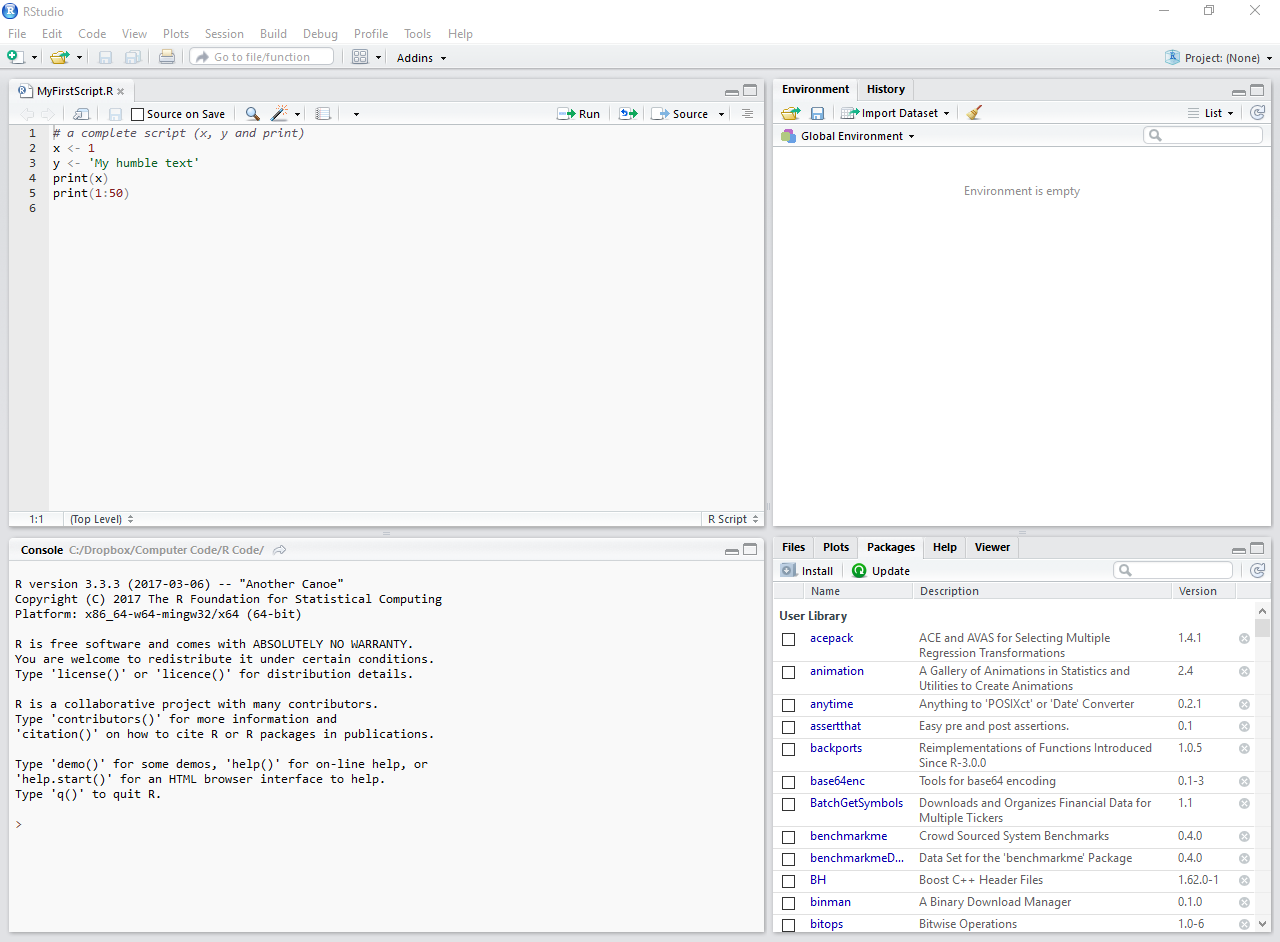
\includegraphics[width=1\linewidth]{figs/RStudio_example_script} 

}

\caption{Example of a R script}\label{fig:example-script}
\end{figure}

After pasting all the commands in the editor, save the \emph{.R} file to
a personal folder where you have read and write permissions. One
possibility is to save it in the \texttt{My\ Documents} folder with a
name like \texttt{\textquotesingle{}MyFirstRScript.R\textquotesingle{}}.
This saved file, which at the moment does nothing special, records the
steps of a simple algorithm that creates several objects and shows their
content. In the future, this file can take an expressive size by
containing all stages of the data analysis such as importing data,
cleaning it, performing the data analysis and exporting tables and
figures.

In RStudio, there are some predefined and time-saving shortcuts for
running code from the editor. To execute an entire script, simply press
\texttt{control\ +\ shift\ +\ s}. This is the \emph{source} command.
With RStudio open, I suggest testing this key combination and checking
how the code saved in a \emph{.R} file is executed. The output of the
script is shown in the prompt of R. The result in RStudio should look
like Figure \ref{fig:example-script-source}. \index{source}

\begin{figure}[!htbp]

{\centering 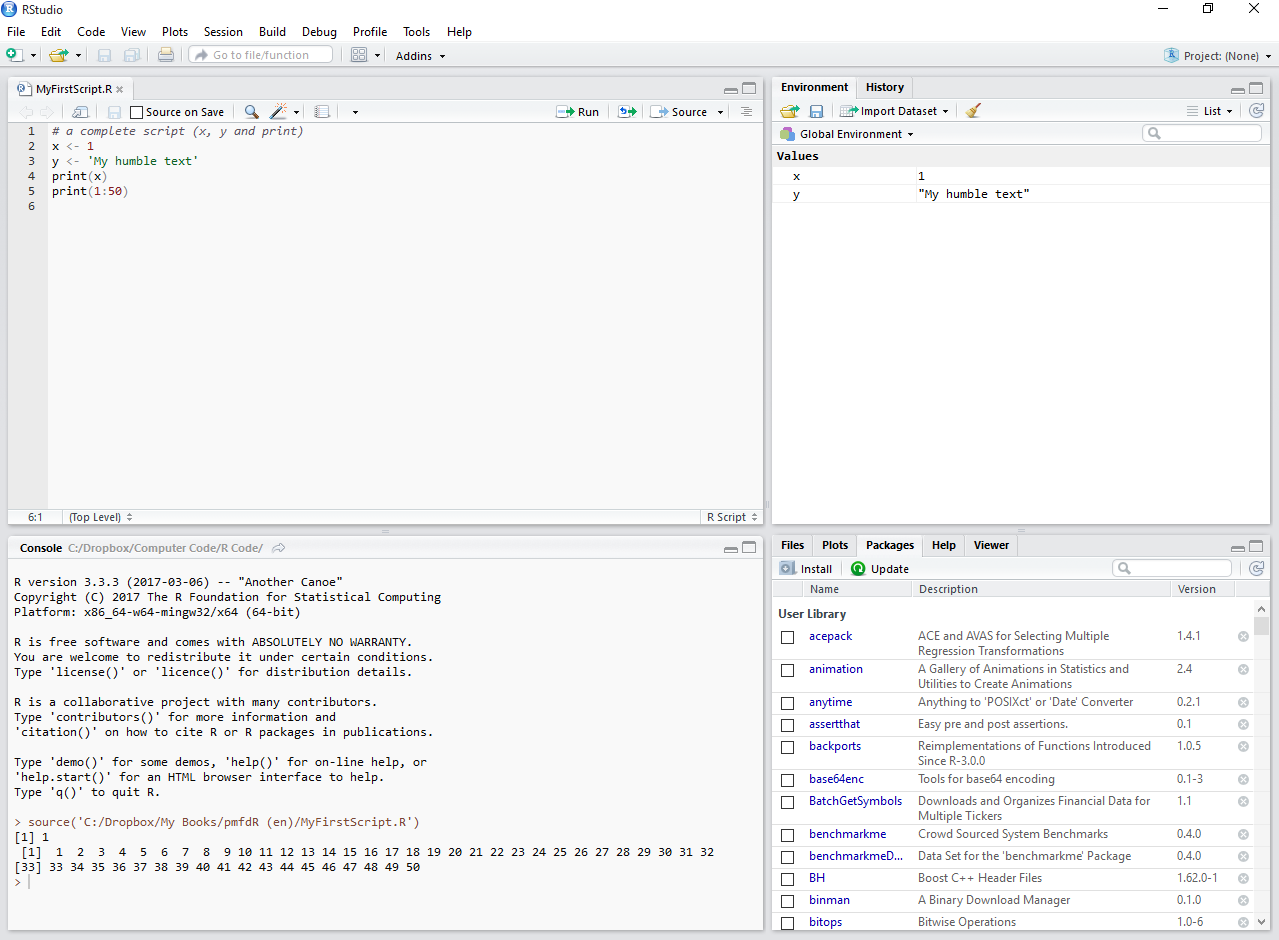
\includegraphics[width=1\linewidth]{figs/RStudio_example_script_source} 

}

\caption{Example of a R script after execution}\label{fig:example-script-source}
\end{figure}

Another very useful command is code execution by the lines. In this
case, the whole file is not executed, but only the line where the cursor
is located. For that, just press \texttt{control\ +\ enter}. This
shortcut is very useful in developing scripts because it allows each
line of the code to be tested before running the entire program. As an
example of usage, point the cursor to the \texttt{print(x)} line and
press \texttt{control\ +\ enter}. As you will notice, only the line
\texttt{print(x)} was executed. Therefore, before running the whole
script, you can test it line by line and check for possible errors.

Next, I highlight these and other RStudio shortcuts, which are also very
useful.

\begin{itemize}
\tightlist
\item
  \textbf{control + shift + s}: executes (source) the current RStudio
  file;
\item
  \textbf{control + shift + enter}: executes the current file with echo,
  showing the commands on the prompt;
\item
  \textbf{control + enter}: executes the selected line, showing
  on-screen commands;
\item
  \textbf{control + shift + b}: executes the codes from the beginning of
  the file to the current line where the cursor is;
\item
  \textbf{control + shift + e}: executes the codes of the lines where
  the cursor is until the end of the file.
\end{itemize}

My suggestion is to use these shortcuts from day one. They greatly
facilitate the use of the program. For those who like to use the
\emph{mouse}, an alternate way to execute code is to click the
\emph{source} button in the upper-right corner of the text editor. If
you want to set your own shortcuts in RStudio, go to option, ``Tools''
and ``Modify Keyboard Shortcuts''. One suggestion here is to set the
\emph{source} command to F5, which is used by several other software as
an ``execute'' shortcut.

If you want to run code in a \emph{.R} file within another .R file, you
can use the \texttt{source} command. For example, imagine that you have
a main script with your data analysis and another script that performs
some support operation such as importing data to R. These operations
have been dismembered as a way of organizing the code.
\index{base!source}

To run the support \emph{script}, just call it with function
\texttt{source} in the main script, as in the following code:

\begin{Shaded}
\begin{Highlighting}[]
\CommentTok{# execute import script}
\KeywordTok{source}\NormalTok{(}\StringTok{'import-data.R'}\NormalTok{)}
\end{Highlighting}
\end{Shaded}

In this case, all code in \texttt{import-data.R} will be executed. This
is equivalent to manually opening file \texttt{import-data.R} and
hitting \emph{control + shift + s}.

\section{Testing and Debugging Code}\label{testing-and-debugging-code}

The development of code follows a cycle. At first, you will write a
command line on a script, try it using \emph{control + enter} and check
the output. A new line of code is written once the previous line worked
as expected. A moving cycle is clear, writing code is followed by line
execution, followed by result checking, modify and repeat if necessary.
This is a normal process. You need to make sure that every line of code
is correctly specified before moving to the next one.

When you are trying to find an error in a preexisting script, R offers
some tools for controlling and assessing its execution. This is
specially useful when you have a long and complicated script. The
simplest and easiest tool that R and RStudio offers is code breakpoint.
In RStudio, you can click in the left side of the script editor and a
red circle will appear, as in Figure \ref{fig:example-debug}.

\begin{figure}[!htbp]

{\centering 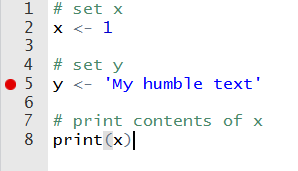
\includegraphics[width=0.75\linewidth]{figs/RStudio_example_debug} 

}

\caption{Example of breakpoint in an R script}\label{fig:example-debug}
\end{figure}

This red circle indicate a code breakpoint that will force the code to
stop at that line. You can use it to test existing code and check its
objects at a certain part of the execution. When the execution hits the
breakpoint, the prompt will change to
\texttt{Browse{[}1{]}\textgreater{}} and you'll be able to try new code
of verify the content of the objects. From the Console, you have the
option to continue the execution to the next breakpoint or stop it. The
same result can be achieved using function \texttt{browser}. Have a
look:

\begin{Shaded}
\begin{Highlighting}[]
\CommentTok{# set x}
\NormalTok{x <-}\StringTok{ }\DecValTok{1}

\CommentTok{# set y}
\KeywordTok{browser}\NormalTok{()}
\NormalTok{y <-}\StringTok{ 'My humble text'}

\CommentTok{# print contents of x}
\KeywordTok{print}\NormalTok{(x)}
\end{Highlighting}
\end{Shaded}

The practical result is the same as using RStudio's red circle, but it
gives you more control for the case of several commands in the same
line.

\section{Creating Simple Objects}\label{creating-simple-objects}

One of the most basic and most used commands in R is the creation of
objects. As shown in previous sections, you can define an object using
the \texttt{\textless{}-} command, which is verbally translated to
\emph{assign}. For example, consider the following code: \index{assign}

\begin{Shaded}
\begin{Highlighting}[]
\CommentTok{# set x}
\NormalTok{x <-}\StringTok{ }\DecValTok{123}

\CommentTok{# set x, y and z in one line}
\NormalTok{my.x <-}\StringTok{ }\DecValTok{1}\NormalTok{ ; my.y <-}\StringTok{ }\DecValTok{2}\NormalTok{; my.z <-}\StringTok{ }\DecValTok{3}
\end{Highlighting}
\end{Shaded}

We can read this code as \emph{the value 123 is assigned to x}. The
direction of the arrow defines where the value is stored. For example,
using \texttt{123\ -\textgreater{}\ x} also works, although this is not
recommended as the code becomes less readable. Also notice that you can
create objects within the same line by separating the commands using a
semi-colon.

The use of an arrow symbol \texttt{\textless{}-} for object definition
is specific to R. The reason for this choice was that, at the time of
conception of the \emph{S} language, keyboards with a key that directly
defined the arrow symbol were available and used. This means that the
programmer only had to hit one key in the keyboard in order to set the
arrow symbol. Modern keyboards, however, do not have this format any
more. If you find it troublesome to use this symbol, you can use
shortcuts as well. In \emph{Windows}, the shortcut for the the symbol
\texttt{\textless{}-} is \texttt{alt} plus \texttt{-}.

You can also use the \texttt{=} symbol to define objects such as in
\texttt{x\ =\ 123}, but the use of \texttt{=} with this specific purpose
is not recommended. The symbol of equality has a special use within the
definition of function arguments. This case will be better explained and
demonstrated in future section.

The name of the object is important in R. With the exception of very
specific cases, the user can name objects as he likes. This freedom,
however, can be a problem. It is desirable to always give short names
that make sense to the content of the script and which are simple to
understand. This facilitates the understanding of the code by other
users and is part of the suggested set of rules for structuring code.
Note that all objects created in this book have nomenclature in English
and specific formatting, where the white space between nouns are
replaced by a dot, as in \texttt{my.x\ \textless{}-\ 1} and
\texttt{name.of.file\ \textless{}-\ \textquotesingle{}my\_file.csv\textquotesingle{}}.

R executes the code looking for objects available in the environment,
including functions. Be aware that R is case sensitive, that is, object
\texttt{m} is different than \texttt{M}. If we try to access an object
that does not exist, R will return an error message and stop the
execution. Have a look:

\begin{Shaded}
\begin{Highlighting}[]
\KeywordTok{print}\NormalTok{(z)}
\end{Highlighting}
\end{Shaded}

\begin{verbatim}
## Error in print(z): object 'z' not found
\end{verbatim}

The error occurred because object \texttt{z} does not exist in the
current environment. If we create a variable \texttt{z} as
\texttt{z\ \textless{}-\ 321} and repeat the command \texttt{print(z)},
we will not have the same error message.

\section{Creating Vectors}\label{creating-vectors}

In the previous examples, we have created simple objects such as
\texttt{x\ \textless{}-\ 1} and
\texttt{x\ \textless{}-\ \textquotesingle{}abc\textquotesingle{}}. While
this is sufficient to demonstrate the basic commands in R, in practice,
such commands are very limited. A real problem of data analysis will
certainly have a greater volume of information.

One of the most used procedures in R is the creation of atomic vectors.
These are objects that can have several elements. All elements of an
atomic vector must have the same class, which justifies its
\emph{atomic} property. An example would be the representation of a
series of daily stock prices as an atomic vector of the class
\texttt{numeric}. Once you have a vector, you can manipulate it anyway
you want.

Atomic vectors are created in R using the \texttt{c} command, which
comes from the verb \emph{combine}. For example, if we wanted to combine
the values 1, 2 and 3 in one object, we could do it with the following
command: \index{base!c}

\begin{Shaded}
\begin{Highlighting}[]
\CommentTok{# create numeric atomic vector}
\NormalTok{x <-}\StringTok{ }\KeywordTok{c}\NormalTok{(}\DecValTok{1}\NormalTok{,}\DecValTok{2}\NormalTok{,}\DecValTok{3}\NormalTok{)}

\CommentTok{# print it}
\KeywordTok{print}\NormalTok{(x)}
\end{Highlighting}
\end{Shaded}

\begin{verbatim}
## [1] 1 2 3
\end{verbatim}

This command works the same way for any other class of object, such as
\emph{character}:

\begin{Shaded}
\begin{Highlighting}[]
\CommentTok{# create character atomic vector}
\NormalTok{y <-}\StringTok{ }\KeywordTok{c}\NormalTok{(}\StringTok{'text 1'}\NormalTok{, }\StringTok{'text 2'}\NormalTok{, }\StringTok{'text 3'}\NormalTok{, }\StringTok{'text 4'}\NormalTok{)}

\CommentTok{# print it}
\KeywordTok{print}\NormalTok{(y)}
\end{Highlighting}
\end{Shaded}

\begin{verbatim}
## [1] "text 1" "text 2" "text 3" "text 4"
\end{verbatim}

The only restriction on the use of the \texttt{c} command is that all
elements must have the same class. If we insert data from different
classes in a call to \texttt{c()}, R will try to mutate all elements
into the same class following its own logic. If the conversion of all
elements to a single class is not possible, an error message is
returned. Note the following example, where numeric values are set in
the first and second element of \texttt{x} and a character in the last
element.

\begin{Shaded}
\begin{Highlighting}[]
\CommentTok{# a mixed vector}
\NormalTok{x <-}\StringTok{ }\KeywordTok{c}\NormalTok{(}\DecValTok{1}\NormalTok{, }\DecValTok{2}\NormalTok{, }\StringTok{'3'}\NormalTok{)}

\CommentTok{# print result of forced conversion}
\KeywordTok{print}\NormalTok{(x)}
\end{Highlighting}
\end{Shaded}

\begin{verbatim}
## [1] "1" "2" "3"
\end{verbatim}

The values of \texttt{x} are all of type \texttt{character}. The use of
\texttt{class} command confirms this result:

\begin{Shaded}
\begin{Highlighting}[]
\CommentTok{# print class of x}
\KeywordTok{class}\NormalTok{(x)}
\end{Highlighting}
\end{Shaded}

\begin{verbatim}
## [1] "character"
\end{verbatim}

\section{Knowing Your Environment}\label{knowing-your-environment}

After using various commands, further development of the script requires
you to understand what objects are available and what is their content.
You can find this information simply by looking at the upper right
screen of RStudio. However, there is a command that shows the same
information in the prompt. In order to know what objects are currently
available in R's memory, you can use command \texttt{ls}. Note the
following example: \index{base!ls}

\begin{Shaded}
\begin{Highlighting}[]
\CommentTok{# set some objects}
\NormalTok{x <-}\StringTok{ }\DecValTok{1}
\NormalTok{y <-}\StringTok{ }\DecValTok{2}
\NormalTok{z <-}\StringTok{ }\DecValTok{3}

\CommentTok{# print all objects in the environment}
\KeywordTok{print}\NormalTok{(}\KeywordTok{ls}\NormalTok{())}
\end{Highlighting}
\end{Shaded}

\begin{verbatim}
## [1] "x" "y" "z"
\end{verbatim}

The objects \texttt{x}, \texttt{y} and \texttt{z} were created and are
available in the current working environment. If we had other objects,
they would also appear in the output to \texttt{ls}. Notice that object
returned from \texttt{ls} is a \texttt{character} vector.

To display the content of each object, just enter the names of objects
and press \texttt{enter} in the \emph{prompt}:

\begin{Shaded}
\begin{Highlighting}[]
\CommentTok{# print objects by their name}
\NormalTok{x}
\end{Highlighting}
\end{Shaded}

\begin{verbatim}
## [1] 1
\end{verbatim}

\begin{Shaded}
\begin{Highlighting}[]
\NormalTok{y}
\end{Highlighting}
\end{Shaded}

\begin{verbatim}
## [1] 2
\end{verbatim}

\begin{Shaded}
\begin{Highlighting}[]
\NormalTok{z}
\end{Highlighting}
\end{Shaded}

\begin{verbatim}
## [1] 3
\end{verbatim}

Typing the object name on the screen has the same effect as using the
\texttt{print} command. In fact, when executing the sole name of a
variable in the prompt or script, R internally passes the object to the
\texttt{print} function.

In R, all objects belong to a class. As previously mentioned, to find
the class of an object, simply use the \texttt{class} function. In the
following example, \texttt{x} is an object of the class
\texttt{numeric}, \texttt{y} is a text (\texttt{character}) object and
\texttt{my.fct} is a function object. \index{base!class}

\begin{Shaded}
\begin{Highlighting}[]
\CommentTok{# set objects}
\NormalTok{x <-}\StringTok{ }\DecValTok{1}
\NormalTok{y <-}\StringTok{ 'a'}
\NormalTok{my.fct <-}\StringTok{ }\ControlFlowTok{function}\NormalTok{()\{\}}

\CommentTok{# print their classes}
\KeywordTok{print}\NormalTok{(}\KeywordTok{class}\NormalTok{(x))}
\end{Highlighting}
\end{Shaded}

\begin{verbatim}
## [1] "numeric"
\end{verbatim}

\begin{Shaded}
\begin{Highlighting}[]
\KeywordTok{print}\NormalTok{(}\KeywordTok{class}\NormalTok{(y))}
\end{Highlighting}
\end{Shaded}

\begin{verbatim}
## [1] "character"
\end{verbatim}

\begin{Shaded}
\begin{Highlighting}[]
\KeywordTok{print}\NormalTok{(}\KeywordTok{class}\NormalTok{(my.fct))}
\end{Highlighting}
\end{Shaded}

\begin{verbatim}
## [1] "function"
\end{verbatim}

Another way to learn more about an object is to check their textual
representation. Every object in R has a textual representation and we
can find it with function \texttt{str}: \index{base!str}

\begin{Shaded}
\begin{Highlighting}[]
\CommentTok{# print the textual representation of a vector}
\KeywordTok{print}\NormalTok{(}\KeywordTok{str}\NormalTok{(}\DecValTok{1}\OperatorTok{:}\DecValTok{10}\NormalTok{))}
\end{Highlighting}
\end{Shaded}

\begin{verbatim}
##  int [1:10] 1 2 3 4 5 6 7 8 9 10
## NULL
\end{verbatim}

This function is particularly useful when trying to understand the
details of a more complex object, such as a \texttt{dataframe}. We will
learn more about using function \texttt{str} for learning the contents
of a \texttt{dataframe} in chapter \ref{importing}.

\section{Displaying and Formatting
Output}\label{displaying-and-formatting-output}

So far, we saw that you can show the value of an R object on the screen
in two ways. You can either enter its name in the prompt or use the
\texttt{print} function. Explaining it further, the \texttt{print}
function focuses on the presentation of objects and can be customized
for any type. For example, if we had an object of a class called
\texttt{MyTable} to represent a specific type of table, we could create
a function called \texttt{print.MyTable} that would show a table on the
screen with a special format for the rows and column names. Function
\texttt{print}, therefore, is oriented towards presenting objects and
the user can customize it for different classes. The \texttt{base}
package, which is automatically initialized with R, contains several
\texttt{print} function for various kinds of objects.

However, there are other specific functions to display text in the
prompt. The main one is \texttt{cat} (\emph{concatenate and print}).
This function takes a text as input, processes it for specific symbols
and displays the result on the screen. Function \texttt{cat} is more
powerful and customizable than \texttt{print}. \index{base!cat}

For example, if we wanted to show the text,
\texttt{The\ value\ of\ x\ is\ equal\ to\ 2} on screen using a numerical
object, we could do it as follows:

\begin{Shaded}
\begin{Highlighting}[]
\CommentTok{# set x}
\NormalTok{x <-}\StringTok{ }\DecValTok{2}

\CommentTok{# print customized message}
\KeywordTok{cat}\NormalTok{(}\StringTok{'The value of x is'}\NormalTok{, x)}
\end{Highlighting}
\end{Shaded}

\begin{verbatim}
## The value of x is 2
\end{verbatim}

You can also customize the screen output using specific commands. For
example, if we wanted to break a line in the screen output, we could do
it through the use of the reserved character \texttt{\textbackslash{}n}:

\begin{Shaded}
\begin{Highlighting}[]
\CommentTok{# set text with break line}
\NormalTok{my.text <-}\StringTok{ ' First Line,}\CharTok{\textbackslash{}n}\StringTok{ Second line'}

\CommentTok{# print it}
\KeywordTok{cat}\NormalTok{(my.text)}
\end{Highlighting}
\end{Shaded}

\begin{verbatim}
##  First Line,
##  Second line
\end{verbatim}

Note that the use of \texttt{print} would not result in the same effect
as this command displays the text as it is, without processing it for
specific symbols:

\begin{Shaded}
\begin{Highlighting}[]
\KeywordTok{print}\NormalTok{(my.text)}
\end{Highlighting}
\end{Shaded}

\begin{verbatim}
## [1] " First Line,\n Second line"
\end{verbatim}

Another example in the use of specific commands for text is to add a
\emph{tab} space with the symbol \texttt{\textbackslash{}t}. See an
example next:

\begin{Shaded}
\begin{Highlighting}[]
\CommentTok{# set text with tab}
\NormalTok{my.text <-}\StringTok{ 'A->}\CharTok{\textbackslash{}t}\StringTok{<-B'}

\CommentTok{# concatenate and print it!}
\KeywordTok{cat}\NormalTok{(my.text)}
\end{Highlighting}
\end{Shaded}

\begin{verbatim}
## A->  <-B
\end{verbatim}

We've only scratched the surface on the possible ways to manipulate text
output. Other ways to manipulate text output based on specific symbols
can be found in the
\href{https://cran.r-project.org/doc/manuals/R-lang.html\#Literal-constants}{official
R manual}, available on the book website.

\subsection{Customizing the Output}\label{customizing-the-output}

Another way to customize text output is using specific functions to
manipulate objects of the class \texttt{character}. For that, there are
two very useful functions: \texttt{paste} and \texttt{format}.
\index{base!paste} \index{base!format}

Function \texttt{paste} \emph{glues} a series of objects together. It is
a very useful function, and will be used intensely for the rest of the
examples in this book. Consider the following example:

\begin{Shaded}
\begin{Highlighting}[]
\CommentTok{# set some text objects}
\NormalTok{my.text.}\DecValTok{1}\NormalTok{ <-}\StringTok{ 'I am a text'}
\NormalTok{my.text.}\DecValTok{2}\NormalTok{ <-}\StringTok{ 'very beautiful'}
\NormalTok{my.text.}\DecValTok{3}\NormalTok{ <-}\StringTok{ 'and informative.'}

\CommentTok{# paste all objects together and print}
\KeywordTok{cat}\NormalTok{(}\KeywordTok{paste}\NormalTok{(my.text.}\DecValTok{1}\NormalTok{, my.text.}\DecValTok{2}\NormalTok{, my.text.}\DecValTok{3}\NormalTok{))}
\end{Highlighting}
\end{Shaded}

\begin{verbatim}
## I am a text very beautiful and informative.
\end{verbatim}

The previous result is not far from what we did in the example with the
\texttt{print} function. Note, however, that the \texttt{paste} function
adds a space between each text. If we did not want this space, we could
use function \texttt{paste0} as in:

\begin{Shaded}
\begin{Highlighting}[]
\CommentTok{# example of paste0}
\KeywordTok{cat}\NormalTok{(}\KeywordTok{paste0}\NormalTok{(my.text.}\DecValTok{1}\NormalTok{, my.text.}\DecValTok{2}\NormalTok{, my.text.}\DecValTok{3}\NormalTok{))}
\end{Highlighting}
\end{Shaded}

\begin{verbatim}
## I am a textvery beautifuland informative.
\end{verbatim}

Another very useful possibility with the \texttt{paste} function is to
insert a text or symbol between the junction of texts. For example, if
we wanted to add a comma (\texttt{,}) between each item to be pasted, we
could do this by using the input option \texttt{sep} as follows:

\begin{Shaded}
\begin{Highlighting}[]
\CommentTok{# example using the argument sep}
\KeywordTok{cat}\NormalTok{(}\KeywordTok{paste}\NormalTok{(my.text.}\DecValTok{1}\NormalTok{, my.text.}\DecValTok{2}\NormalTok{, my.text.}\DecValTok{3}\NormalTok{, }\DataTypeTok{sep =} \StringTok{', '}\NormalTok{)) }
\end{Highlighting}
\end{Shaded}

\begin{verbatim}
## I am a text, very beautiful, and informative.
\end{verbatim}

If we had an atomic vector with all elements to be glued in an single
object, we could achieve the same result using the \texttt{collapse}
argument. See an example next.

\begin{Shaded}
\begin{Highlighting}[]
\CommentTok{# set character object }
\NormalTok{my.text <-}\KeywordTok{c}\NormalTok{(}\StringTok{'I am a text'}\NormalTok{, }\StringTok{'very beautiful'}\NormalTok{, }\StringTok{'and informative.'}\NormalTok{)}

\CommentTok{# example of using the collapse argument in paste}
\KeywordTok{cat}\NormalTok{(}\KeywordTok{paste}\NormalTok{(my.text, }\DataTypeTok{collapse =} \StringTok{', '}\NormalTok{)) }
\end{Highlighting}
\end{Shaded}

\begin{verbatim}
## I am a text, very beautiful, and informative.
\end{verbatim}

Going forward, command \texttt{format} is used to format numbers and
dates. It is especially useful when we create tables and we want to
present the numbers in a visually appealing way. By definition, R
presents a set number of digits after the decimal point:
\index{base!format}

\begin{Shaded}
\begin{Highlighting}[]
\CommentTok{# example of decimal points in R}
\KeywordTok{cat}\NormalTok{(}\DecValTok{1}\OperatorTok{/}\DecValTok{3}\NormalTok{)}
\end{Highlighting}
\end{Shaded}

\begin{verbatim}
## 0.3333333
\end{verbatim}

If we wanted only two digits on the screen, we could use the following
code:

\begin{Shaded}
\begin{Highlighting}[]
\CommentTok{# example of using format on numerical objects}
\KeywordTok{cat}\NormalTok{(}\KeywordTok{format}\NormalTok{(}\DecValTok{1}\OperatorTok{/}\DecValTok{3}\NormalTok{, }\DataTypeTok{digits=}\DecValTok{2}\NormalTok{))}
\end{Highlighting}
\end{Shaded}

\begin{verbatim}
## 0.33
\end{verbatim}

Likewise, if we wanted to use a scientific format in the display, we
could do the following:

\begin{Shaded}
\begin{Highlighting}[]
\CommentTok{# example of using scientific format}
\KeywordTok{cat}\NormalTok{(}\KeywordTok{format}\NormalTok{(}\DecValTok{1}\OperatorTok{/}\DecValTok{3}\NormalTok{, }\DataTypeTok{scientific=}\OtherTok{TRUE}\NormalTok{))}
\end{Highlighting}
\end{Shaded}

\begin{verbatim}
## 3.333333e-01
\end{verbatim}

Function \texttt{format} has many more options. If you need your numbers
to come out in a specific way, have a look at the help manual for this
function. It is also a generic function and can be used for many types
of objects.

\section{Finding the Size of Objects}\label{finding-the-size-of-objects}

In the practice of programming with R, it is very important to know the
size of the objects being used. Here, size means the number of
individual elements. This information serves not only to assist the
programmer in checking possible code errors, but also to know the length
of iteration procedures such as \emph{loops}, which will be treated in a
later chapter of this book.

In R, the size of an object can be checked with the use of four main
functions: \texttt{length}, \texttt{nrow}, \texttt{ncol} and
\texttt{dim}. \index{base!length} \index{base!nrow} \index{base!ncol}
\index{base!dim}

Function \texttt{length} is intended for objects with a single
dimension, such as atomic vectors:

\begin{Shaded}
\begin{Highlighting}[]
\CommentTok{# create atomic vector}
\NormalTok{x <-}\StringTok{ }\KeywordTok{c}\NormalTok{(}\DecValTok{2}\NormalTok{,}\DecValTok{3}\NormalTok{,}\DecValTok{3}\NormalTok{,}\DecValTok{4}\NormalTok{,}\DecValTok{2}\NormalTok{,}\DecValTok{1}\NormalTok{)}

\CommentTok{# get length of x}
\NormalTok{n <-}\StringTok{ }\KeywordTok{length}\NormalTok{(x)}

\CommentTok{# display message}
\KeywordTok{cat}\NormalTok{(}\StringTok{'The size of x is '}\NormalTok{, n)}
\end{Highlighting}
\end{Shaded}

\begin{verbatim}
## The size of x is  6
\end{verbatim}

For objects with more than one dimension, such as matrices, use
functions \texttt{nrow}, \texttt{ncol} and \texttt{dim} (dimension) to
find the number of rows (first dimension) and the number of columns
(second dimension). See the difference in usage below.

\begin{Shaded}
\begin{Highlighting}[]
\CommentTok{# create a matrix}
\NormalTok{M <-}\StringTok{ }\KeywordTok{matrix}\NormalTok{(}\DecValTok{1}\OperatorTok{:}\DecValTok{20}\NormalTok{, }\DataTypeTok{nrow =} \DecValTok{4}\NormalTok{, }\DataTypeTok{ncol =} \DecValTok{5}\NormalTok{)}

\CommentTok{# print matrix}
\KeywordTok{print}\NormalTok{(M)}
\end{Highlighting}
\end{Shaded}

\begin{verbatim}
##      [,1] [,2] [,3] [,4] [,5]
## [1,]    1    5    9   13   17
## [2,]    2    6   10   14   18
## [3,]    3    7   11   15   19
## [4,]    4    8   12   16   20
\end{verbatim}

\begin{Shaded}
\begin{Highlighting}[]
\CommentTok{# calculate size in different ways}
\NormalTok{my.nrow <-}\StringTok{ }\KeywordTok{nrow}\NormalTok{(M)}
\NormalTok{my.ncol <-}\StringTok{ }\KeywordTok{ncol}\NormalTok{(M)}
\NormalTok{my.n.elements <-}\StringTok{ }\KeywordTok{length}\NormalTok{(M)}

\CommentTok{# display message }
\KeywordTok{cat}\NormalTok{(}\StringTok{'The number of lines in M is '}\NormalTok{, my.nrow)}
\end{Highlighting}
\end{Shaded}

\begin{verbatim}
## The number of lines in M is  4
\end{verbatim}

\begin{Shaded}
\begin{Highlighting}[]
\KeywordTok{cat}\NormalTok{(}\StringTok{'The number of columns in M is '}\NormalTok{, my.ncol)}
\end{Highlighting}
\end{Shaded}

\begin{verbatim}
## The number of columns in M is  5
\end{verbatim}

\begin{Shaded}
\begin{Highlighting}[]
\KeywordTok{cat}\NormalTok{(}\StringTok{'The number of elements in M is '}\NormalTok{, my.n.elements)}
\end{Highlighting}
\end{Shaded}

\begin{verbatim}
## The number of elements in M is  20
\end{verbatim}

The \texttt{dim} function shows the dimension of the object, resulting
in a numeric vector as output. This function should be used when the
object has more than two dimensions. In practice, however, such cases
are rare. An example is given next:

\begin{Shaded}
\begin{Highlighting}[]
\CommentTok{# get dimension of M}
\NormalTok{my.dim <-}\StringTok{ }\KeywordTok{dim}\NormalTok{(M)}

\CommentTok{# print it}
\KeywordTok{print}\NormalTok{(my.dim)}
\end{Highlighting}
\end{Shaded}

\begin{verbatim}
## [1] 4 5
\end{verbatim}

In the case of objects with more than two dimensions, we can use the
\texttt{array} function to create the object and \texttt{dim} to find
its size. Have a look in the next example:

\begin{Shaded}
\begin{Highlighting}[]
\CommentTok{# create an array with three dimensions}
\NormalTok{my.array <-}\StringTok{ }\KeywordTok{array}\NormalTok{(}\DecValTok{1}\OperatorTok{:}\DecValTok{9}\NormalTok{, }\DataTypeTok{dim =} \KeywordTok{c}\NormalTok{(}\DecValTok{3}\NormalTok{,}\DecValTok{3}\NormalTok{,}\DecValTok{3}\NormalTok{))}

\CommentTok{# print it}
\KeywordTok{print}\NormalTok{(my.array)}
\end{Highlighting}
\end{Shaded}

\begin{verbatim}
## , , 1
## 
##      [,1] [,2] [,3]
## [1,]    1    4    7
## [2,]    2    5    8
## [3,]    3    6    9
## 
## , , 2
## 
##      [,1] [,2] [,3]
## [1,]    1    4    7
## [2,]    2    5    8
## [3,]    3    6    9
## 
## , , 3
## 
##      [,1] [,2] [,3]
## [1,]    1    4    7
## [2,]    2    5    8
## [3,]    3    6    9
\end{verbatim}

\begin{Shaded}
\begin{Highlighting}[]
\CommentTok{# display its dimensions}
\KeywordTok{print}\NormalTok{(}\KeywordTok{dim}\NormalTok{(my.array))}
\end{Highlighting}
\end{Shaded}

\begin{verbatim}
## [1] 3 3 3
\end{verbatim}

An important note here is that the use of the functions,
\texttt{length}, \texttt{nrow}, \texttt{dim} and \texttt{ncol} are not
intended to discover the number of letters in a text. This is a common
mistake. For example, if we had a \texttt{character} type of object and
we use the \texttt{length} function, the result would be the following:

\begin{Shaded}
\begin{Highlighting}[]
\CommentTok{# set text object}
\NormalTok{my.char <-}\StringTok{ 'abcde'}

\CommentTok{# print result of length}
\KeywordTok{print}\NormalTok{(}\KeywordTok{length}\NormalTok{(my.char))}
\end{Highlighting}
\end{Shaded}

\begin{verbatim}
## [1] 1
\end{verbatim}

This occurred because the \texttt{length} function returns the number of
elements in an object. In this case, \texttt{my.char} has only one
element. To find out the number of characters in the object, we use the
\texttt{nchar} function as follows: \index{base!nchar}

\begin{Shaded}
\begin{Highlighting}[]
\CommentTok{# find the number of characters in an character object}
\KeywordTok{print}\NormalTok{(}\KeywordTok{nchar}\NormalTok{(my.char))}
\end{Highlighting}
\end{Shaded}

\begin{verbatim}
## [1] 5
\end{verbatim}

\section{Selecting the Elements of an Atomic
Vector}\label{selecting-the-elements-of-an-atomic-vector}

After creating an atomic vector of a class, it is possible that the user
is interested in only one or more elements of it. For example, if we
were updating the value of an investment portfolio, our interest in a
vector containing stock prices is only for the latest price. All other
prices were not relevant to our analysis and therefore could be ignored.

The selection of \emph{pieces} of an atomic vector is called indexing
and it is accomplished with the use of square brackets
(\texttt{{[}\ {]}}). Consider the following example:

\begin{Shaded}
\begin{Highlighting}[]
\CommentTok{# set x}
\NormalTok{my.x <-}\StringTok{ }\KeywordTok{c}\NormalTok{(}\DecValTok{1}\NormalTok{, }\DecValTok{5}\NormalTok{, }\DecValTok{4}\NormalTok{, }\DecValTok{3}\NormalTok{, }\DecValTok{2}\NormalTok{, }\DecValTok{7}\NormalTok{, }\FloatTok{3.5}\NormalTok{, }\FloatTok{4.3}\NormalTok{)}
\end{Highlighting}
\end{Shaded}

If we wanted only the third element of \texttt{my.x}, we use the bracket
operator as follows:

\begin{Shaded}
\begin{Highlighting}[]
\CommentTok{# get third element of x}
\NormalTok{elem.x <-}\StringTok{ }\NormalTok{my.x[}\DecValTok{3}\NormalTok{]}

\CommentTok{# print it}
\KeywordTok{print}\NormalTok{(elem.x)}
\end{Highlighting}
\end{Shaded}

\begin{verbatim}
## [1] 4
\end{verbatim}

The procedure of indexing also works with vectors. If we are only
interested in the last and penultimate values of \texttt{my.x}, we use
the following code:

\begin{Shaded}
\begin{Highlighting}[]
\CommentTok{# get last and penultimate value of my.x}
\NormalTok{piece.x.}\DecValTok{1}\NormalTok{ <-}\StringTok{ }\NormalTok{my.x[ (}\KeywordTok{length}\NormalTok{(my.x)}\OperatorTok{-}\DecValTok{1}\NormalTok{)}\OperatorTok{:}\KeywordTok{length}\NormalTok{(my.x) ]}

\CommentTok{# print it}
\KeywordTok{print}\NormalTok{(piece.x.}\DecValTok{1}\NormalTok{)}
\end{Highlighting}
\end{Shaded}

\begin{verbatim}
## [1] 3.5 4.3
\end{verbatim}

A cautionary note. \textbf{A unique property of the R language is that
if a non existing element is accessed, the program returns the value
\texttt{NA} (\emph{not available})}. See the next example code, where we
attempt to obtain the fourth value of a vector with only three
components.

\begin{Shaded}
\begin{Highlighting}[]
\CommentTok{# set object}
\NormalTok{my.vec <-}\StringTok{ }\KeywordTok{c}\NormalTok{(}\DecValTok{1}\NormalTok{,}\DecValTok{2}\NormalTok{,}\DecValTok{3}\NormalTok{)}

\CommentTok{# print non-existing fourth element}
\KeywordTok{print}\NormalTok{(my.vec[}\DecValTok{4}\NormalTok{])}
\end{Highlighting}
\end{Shaded}

\begin{verbatim}
## [1] NA
\end{verbatim}

It is important to know this behaviour because the lack of treatment of
these errors can lead to problems that are difficult to identify in more
complex code. In other programming languages, attempting to access
non-existing elements generally returns an error and cancels the
execution of the rest of the code. In the case of R, given that access
to non-existent elements does not generate an error or \emph{warning}
message, it is possible that this will create a problem in other parts
of the script as \texttt{NA} objects are contagious. That is, anything
that interacts with \texttt{NA} will also become \texttt{NA}. The user
should pay attention every time that \texttt{NA} values are found
unexpectedly. An inspection in the length and indexation of vectors may
be required.

The use of indices is very useful when you are looking for items of a
vector that satisfy some condition. For example, if we wanted to find
out all values in \texttt{my.x} that are greater than 3, we could use
the following command:

\begin{Shaded}
\begin{Highlighting}[]
\CommentTok{# find all values in my.x that are greater than 3}
\NormalTok{piece.x.}\DecValTok{2}\NormalTok{ <-}\StringTok{ }\NormalTok{my.x[my.x}\OperatorTok{>}\DecValTok{3}\NormalTok{]}

\CommentTok{# print it}
\KeywordTok{print}\NormalTok{(piece.x.}\DecValTok{2}\NormalTok{) }
\end{Highlighting}
\end{Shaded}

\begin{verbatim}
## [1] 5.0 4.0 7.0 3.5 4.3
\end{verbatim}

It is also possible to index elements by more than one condition using
the logical operators \texttt{\&} and \texttt{\textbar{}} (\emph{or}).
For example, if we wanted the values of \texttt{my.x} greater than 2
\textbf{and} lower than 4, we could use the following command:
\index{logical operators}

\begin{Shaded}
\begin{Highlighting}[]
\CommentTok{# find all values of my.x that are greater than 2 and lower then 4}
\NormalTok{piece.x.}\DecValTok{3}\NormalTok{ <-}\StringTok{ }\NormalTok{my.x[ (my.x}\OperatorTok{>}\DecValTok{2}\NormalTok{) }\OperatorTok{&}\StringTok{ }\NormalTok{(my.x}\OperatorTok{<}\DecValTok{4}\NormalTok{) ]}
\KeywordTok{print}\NormalTok{(piece.x.}\DecValTok{3}\NormalTok{)}
\end{Highlighting}
\end{Shaded}

\begin{verbatim}
## [1] 3.0 3.5
\end{verbatim}

Likewise, if we wanted all items that are lower than 3 \textbf{or}
greater than 6, we use:

\begin{Shaded}
\begin{Highlighting}[]
\CommentTok{# find all values of my.x that are lower than 3 or higher than 6}
\NormalTok{piece.x.}\DecValTok{4}\NormalTok{ <-}\StringTok{ }\NormalTok{my.x[ (my.x}\OperatorTok{<}\DecValTok{3}\NormalTok{)}\OperatorTok{|}\NormalTok{(my.x}\OperatorTok{>}\DecValTok{6}\NormalTok{) ]}

\CommentTok{# print it}
\KeywordTok{print}\NormalTok{(piece.x.}\DecValTok{4}\NormalTok{)}
\end{Highlighting}
\end{Shaded}

\begin{verbatim}
## [1] 1 2 7
\end{verbatim}

Moreover, logic indexing also works with the interaction of different
objects. That is, we can use a logical condition in one object to select
items from another:

\begin{Shaded}
\begin{Highlighting}[]
\CommentTok{# set my.x and my.y}
\NormalTok{my.x <-}\StringTok{ }\KeywordTok{c}\NormalTok{(}\DecValTok{1}\NormalTok{,}\DecValTok{4}\NormalTok{,}\DecValTok{6}\NormalTok{,}\DecValTok{8}\NormalTok{,}\DecValTok{12}\NormalTok{)}
\NormalTok{my.y <-}\StringTok{ }\KeywordTok{c}\NormalTok{(}\OperatorTok{-}\DecValTok{2}\NormalTok{,}\OperatorTok{-}\DecValTok{3}\NormalTok{,}\DecValTok{4}\NormalTok{,}\DecValTok{10}\NormalTok{,}\DecValTok{14}\NormalTok{)}

\CommentTok{# find all elements of my.x where my.y is higher than 0}
\NormalTok{my.piece.x <-}\StringTok{ }\NormalTok{my.x[ my.y }\OperatorTok{>}\StringTok{ }\DecValTok{0}\NormalTok{ ]}

\CommentTok{# print it}
\KeywordTok{print}\NormalTok{(my.piece.x)}
\end{Highlighting}
\end{Shaded}

\begin{verbatim}
## [1]  6  8 12
\end{verbatim}

Looking more closely at the indexing process, it is worth noting that,
when we use a data indexing condition, we are in fact creating a
variable of the \texttt{logical} type. This object takes only two
values: \texttt{TRUE} and \texttt{FALSE}. Have a look in the code
presented next, where we create a \texttt{logical} object, print it and
present its class.

\begin{Shaded}
\begin{Highlighting}[]
\CommentTok{# create a logical object}
\NormalTok{my.logical <-}\StringTok{ }\NormalTok{my.y }\OperatorTok{>}\StringTok{ }\DecValTok{0}

\CommentTok{# print it }
\KeywordTok{print}\NormalTok{(my.logical) }
\end{Highlighting}
\end{Shaded}

\begin{verbatim}
## [1] FALSE FALSE  TRUE  TRUE  TRUE
\end{verbatim}

\begin{Shaded}
\begin{Highlighting}[]
\CommentTok{# find its class}
\KeywordTok{class}\NormalTok{(my.logical)}
\end{Highlighting}
\end{Shaded}

\begin{verbatim}
## [1] "logical"
\end{verbatim}

\section{Removing Objects from the
Memory}\label{removing-objects-from-the-memory}

After creating several variables, the R environment can become full of
content that's already been used and is dispensable. In this case, it is
desirable to clear the memory to erase objects that are no longer
needed. Generally, this is accomplished at the beginning of a script, so
that every time the script runs, the memory will be cleared before any
calculation. In addition to cleaning the computer's memory, it also
helps to avoid possible errors in the code. In most cases, cleaning the
working environment should be performed only once at the beginning of
the script.

For example, given an object \texttt{x}, we can delete it from memory
with the command \texttt{rm}, as shown next: \index{base!rm}

\begin{Shaded}
\begin{Highlighting}[]
\CommentTok{# set x}
\NormalTok{x <-}\StringTok{ }\DecValTok{1}

\CommentTok{# print all available objects}
\KeywordTok{ls}\NormalTok{()}
\end{Highlighting}
\end{Shaded}

\begin{verbatim}
##  [1] "elem.x"        "M"             "my.array"     
##  [4] "my.char"       "my.dim"        "my.engine"    
##  [7] "my.fct"        "my.logical"    "my.n.elements"
## [10] "my.ncol"       "my.nrow"       "my.out.width" 
## [13] "my.piece.x"    "my.str"        "my.text"      
## [16] "my.text.1"     "my.text.2"     "my.text.3"    
## [19] "my.vec"        "my.x"          "my.y"         
## [22] "my.z"          "n"             "piece.x.1"    
## [25] "piece.x.2"     "piece.x.3"     "piece.x.4"    
## [28] "stay.quiet"    "x"             "y"            
## [31] "z"
\end{verbatim}

\begin{Shaded}
\begin{Highlighting}[]
\CommentTok{# remove x}
\KeywordTok{rm}\NormalTok{(}\StringTok{'x'}\NormalTok{)}

\CommentTok{# print again all available objects}
\KeywordTok{ls}\NormalTok{()}
\end{Highlighting}
\end{Shaded}

\begin{verbatim}
##  [1] "elem.x"        "M"             "my.array"     
##  [4] "my.char"       "my.dim"        "my.engine"    
##  [7] "my.fct"        "my.logical"    "my.n.elements"
## [10] "my.ncol"       "my.nrow"       "my.out.width" 
## [13] "my.piece.x"    "my.str"        "my.text"      
## [16] "my.text.1"     "my.text.2"     "my.text.3"    
## [19] "my.vec"        "my.x"          "my.y"         
## [22] "my.z"          "n"             "piece.x.1"    
## [25] "piece.x.2"     "piece.x.3"     "piece.x.4"    
## [28] "stay.quiet"    "y"             "z"
\end{verbatim}

Note that after executing the command
\texttt{rm(\textquotesingle{}x\textquotesingle{})}, the value of
\texttt{x} is no longer available in the output of \texttt{ls()}. In
practical situations, however, it is desirable to clean up all the
memory used by all objects created in R. We can achieve this goal with
the following code:

\begin{Shaded}
\begin{Highlighting}[]
\KeywordTok{rm}\NormalTok{(}\DataTypeTok{list=}\KeywordTok{ls}\NormalTok{())}
\end{Highlighting}
\end{Shaded}

The term \texttt{list} in \texttt{rm(list=ls())} is a function argument
of \texttt{rm} that defines which objects will be deleted. The
\texttt{ls()} command shows all the currently available objects.
Therefore, by chaining together both commands, we erase all current
objects available in the environment. As mentioned before, it is good
programming policy to always start the script by clearing the memory.
However, you should only wipe out all of R's memory if you have already
saved the results of interest or if you can replicate them.

\section{Displaying and Setting the Working
Directory}\label{displaying-and-setting-the-working-directory}

Like other programming platforms, \textbf{R always works in a
directory}. If no directory is set, a default value is used when R
starts up. It is based on the current directory that R searches for
files to load data or other R scripts. It is in this directory that R
saves any output we want if we do not explicitly define an address on
the computer. This output can be a graphic file, text or a spreadsheet
like file. A good programming policy is to change the working directory
to the same place where the \emph{script} is located. In chapter
\ref{research-scripts} we discuss the topic of file and folder
organization.

To show the current working directory, use function \texttt{getwd}:
\index{base!getwd}

\begin{Shaded}
\begin{Highlighting}[]
\CommentTok{# get current dir}
\NormalTok{my.dir <-}\StringTok{ }\KeywordTok{getwd}\NormalTok{()}

\CommentTok{# display it}
\KeywordTok{print}\NormalTok{(my.dir)}
\end{Highlighting}
\end{Shaded}

\begin{verbatim}
## [1] "C:/Dropbox/My Books/pafdR (en)/Book Content"
\end{verbatim}

The result of the previous code shows the folder in which this book was
written and compiled. As you can see, the book files are saved in a
subfolder of my Dropbox directory. From the path, you should also
realize that I'm working in a Windows OS. The root directory
\texttt{C:/} gives that information away.

The change of working directory is performed with the \texttt{setwd}
command. For example, if we wanted to change our working directory to
\emph{C:/My Research/}, simply type in the \emph{prompt}:
\index{base!setwd}

\begin{Shaded}
\begin{Highlighting}[]
\CommentTok{# set where to change directory}
\NormalTok{my.d <-}\StringTok{ 'C:/My Research/'}

\CommentTok{# change it}
\KeywordTok{setwd}\NormalTok{(my.d)}
\end{Highlighting}
\end{Shaded}

As for simple cases such as the above, remembering the directory name is
easy. In practical cases, however, the working directory can be in a
deeper directory of the file system. In this situation, an efficient
strategy to locate the path is to use a file explorer, like Windows
\emph{explorer}. To do so, open the \emph{explorer} application and
navigate to the location where you want to work with your \emph{script}.
Place the cursor in the address bar and select the whole path. Press
\emph{control + c} to copy the address to the clipboard. Go back to your
code and paste it in. \textbf{An important step here: Windows uses the
backslash to set addresses on the computer, while the R uses the forward
slash}. If you try to use backslashes, an error is displayed on the
screen. See the following example.

\begin{Shaded}
\begin{Highlighting}[]
\CommentTok{# set directory (WRONG WAY)}
\NormalTok{my.d <-}\StringTok{ 'C:\textbackslash{}My Research}\CharTok{\textbackslash{}'}
\end{Highlighting}
\end{Shaded}

\begin{Shaded}
\begin{Highlighting}[]
\KeywordTok{cat}\NormalTok{(}\StringTok{"##Error: '}\CharTok{\textbackslash{}\textbackslash{}}\StringTok{M' is an unrecognized escape in character string"}\NormalTok{)}
\end{Highlighting}
\end{Shaded}

This message means that R was not able to understand the use of
backslashes. This is a reserved symbol for macros and should not be used
anywhere in a code. Therefore, after copying the address, modify all
backslashes to forward slashes, as in the following code:

\begin{Shaded}
\begin{Highlighting}[]
\CommentTok{# set directory (CORRECT WAY)}
\NormalTok{my.d <-}\StringTok{ 'C:/My Research/'}

\CommentTok{# change dir}
\KeywordTok{setwd}\NormalTok{(my.d)}
\end{Highlighting}
\end{Shaded}

You can also use double backslashes
\texttt{\textbackslash{}\textbackslash{}} but this is not recommended as
it is not compatible with other operating systems.

Another important information here is that you can also use relative
paths. For example, if you are working in a folder that contains a
subdirectory called \texttt{Data}, you can enter this subfolder with the
code:

\begin{Shaded}
\begin{Highlighting}[]
\CommentTok{# change to subfolder}
\KeywordTok{setwd}\NormalTok{(}\StringTok{'Data'}\NormalTok{)}
\end{Highlighting}
\end{Shaded}

Another possibility is to go to a previous level of directory using
\texttt{..}, as in:

\begin{Shaded}
\begin{Highlighting}[]
\CommentTok{# change to previous level}
\KeywordTok{setwd}\NormalTok{(}\StringTok{'..'}\NormalTok{)}
\end{Highlighting}
\end{Shaded}

So, if you are working in the directory \texttt{C:/My\ Research/} and
execute the command
\texttt{setwd(\textquotesingle{}..\textquotesingle{})}, the current
folder becomes \texttt{C:/}, which is one level above
\texttt{C:/My\ Research/}.

Another, more modern, way of setting the directory is to use RStudio API
functions. This is a set of functions that only work inside RStudio and
provides information about current file, project and many more. To find
out the path of the current R script being edited in RStudio and set the
working directory to there, you can write:

\begin{Shaded}
\begin{Highlighting}[]
\NormalTok{my.path <-}\StringTok{ }\KeywordTok{dirname}\NormalTok{(rstudioapi}\OperatorTok{::}\KeywordTok{getActiveDocumentContext}\NormalTok{()}\OperatorTok{$}\NormalTok{path)}
\KeywordTok{setwd}\NormalTok{(my.path)}
\end{Highlighting}
\end{Shaded}

This way, the script will change the directory to its own location, no
matter where you copy it. Be aware, however, that this trick only works
in RStudio script editor and within a saved file. It will not work from
the prompt.

\section{Cancelling Code Execution}\label{cancelling-code-execution}

Whenever R is running some code, a visual cue in the shape of a small
red circle in the right corner of the \emph{prompt} will appear. If you
read it, the text shows the \emph{stop} word. This button is not only an
indicator for running code but also a shortcut for cancelling its
execution. Another way to cancel an execution is to point the mouse to
the \emph{prompt} and press the \emph{escape} (\emph{esc}) button from
the keyboard.

To try it out, run the next chunk of code in RStudio and cancel its
execution using \emph{esc}.

\begin{Shaded}
\begin{Highlighting}[]
\ControlFlowTok{for}\NormalTok{ (i }\ControlFlowTok{in} \DecValTok{1}\OperatorTok{:}\DecValTok{100}\NormalTok{) \{}
  \KeywordTok{cat}\NormalTok{(}\StringTok{'}\CharTok{\textbackslash{}n}\StringTok{Running code (please make it stop by hitting esc!)'}\NormalTok{)}
  \KeywordTok{Sys.sleep}\NormalTok{(}\DecValTok{1}\NormalTok{)}
\NormalTok{\}}
\end{Highlighting}
\end{Shaded}

In the previous code, we used a \texttt{for} loop to display the message
\texttt{\textquotesingle{}\textbackslash{}nRunning\ code\ (please\ make\ it\ stop\ by\ hitting\ esc!)\textquotesingle{}}
every second. For now, do not worry about the code and functions used in
the example. We will discuss the use of loops chapter \ref{programming}.

\section{Code Comments}\label{code-comments}

In R, comments are set using the hash tag symbol \texttt{\#}. Anything
after this symbol will not be processed by R. This gives you freedom to
write whatever you want within the script. An example:

\begin{Shaded}
\begin{Highlighting}[]
\CommentTok{# this is a comment (R will not parse it)}
\CommentTok{# this is another comment (R will not parse it)}

\NormalTok{x <-}\StringTok{ 'abc'} \CommentTok{# this is an inline comment }
\end{Highlighting}
\end{Shaded}

Comments are a way to communicate any important information that cannot
be directly inferred from the code. In general, you should avoid using
comments that are too obvious or too generic. For example:

\begin{Shaded}
\begin{Highlighting}[]
\CommentTok{# read csv file}
\NormalTok{df <-}\StringTok{ }\KeywordTok{read.csv}\NormalTok{(}\StringTok{'MyDataFile.csv'}\NormalTok{)}
\end{Highlighting}
\end{Shaded}

As you can see, it is quite obvious from line
\texttt{df\ \textless{}-\ read.csv(\textquotesingle{}MyDataFile.csv)}
that the code is reading a .csv file. The name of the function already
states that. So, the comment was not a good one as it did not add any
new information to the user. A better approach at commenting would be to
set the author, description of script and better explain the origin and
last update of the data file. Have a look:

\begin{Shaded}
\begin{Highlighting}[]
\CommentTok{# Script for analyzing a dataset}
\CommentTok{# Author: Mr data analyst (dontspamme@emailprovider.com)}
\CommentTok{# Last script update: 2017-03-10}
\CommentTok{#}
\CommentTok{# File downloaded from www.sitewithdatafiles.com/data-files/}
\CommentTok{# The description of the data goes here}
\CommentTok{# Last file update: 2017-03-10}
\NormalTok{df <-}\StringTok{ }\KeywordTok{read.csv}\NormalTok{(}\StringTok{'MyDataFile.csv'}\NormalTok{)}
\end{Highlighting}
\end{Shaded}

So, by reading the comments, the user will know the purpose of the
script, who wrote it and the date of the last edit. It also includes the
origin of the data file and the date of the latest update. If the user
wants to update the data, all he has to do is to go to the referred
website and download the new file. If the datafile is updated, a new
date should be placed in ``Last file update''.

Another use of comments is to set sections in the code, such as in:

\begin{Shaded}
\begin{Highlighting}[]
\CommentTok{# Script for analyzing a dataset}
\CommentTok{# Author: Mr data analyst (dontspamme@emailprovider.com)}
\CommentTok{# Last script update: 2017-03-10}
\CommentTok{#}
\CommentTok{# File downloaded from www.sitewithdatafiles.com/data-files/}
\CommentTok{# The description of the data goes here}
\CommentTok{# Last file update: 2017-03-10}
\NormalTok{...}

\CommentTok{# Clean data}
\CommentTok{# - remove outliers}
\CommentTok{# - remove unnecessary columns}

\NormalTok{...}

\CommentTok{# Report results}
\CommentTok{# - remove outliers}
\CommentTok{# - remove unnecessary columns}

\NormalTok{...}
\end{Highlighting}
\end{Shaded}

This way, once you need to change a particular part of the code, you can
look for the related section in the comments. If you share code with
other people, you'll soon realize that comments are essential and
expected. They help transmit information that is not available from the
code. A note here, throughout the book you'll see that the code comments
are, most of the time, a bit obvious. This was intentional as clear and
direct messages are important for new users, which is part of the
audience of this book.

\section{Looking for Help}\label{looking-for-help}

A common task in the use of R is to seek help. Even advanced users often
seek instructions on specific tasks, whether it is to better understand
the details of some functions or simply to study a new procedure. The
use of the R help system is part of everyday routine with the software.

You can get help by using the \emph{help} panel in RStudio or directly
from the \emph{prompt}. Simply enter the question mark next to the
object on which you want help, as in \texttt{?mean}. In this case,
object \texttt{mean} is a function and the use of the \texttt{help}
command will open a panel on the right side of RStudio.
\index{base!help}

In R, the help screen of a function is the same as shown in Figure
\ref{fig:ExampleHelp}. It presents a general description of the
function, explains its input arguments and the format of the output. The
help screen follows with references and suggestions for other related
functions. More importantly, examples of usage are given last and can be
copied to the prompt or script in order to accelerate the learning
process.

\begin{figure}[!htbp]

{\centering 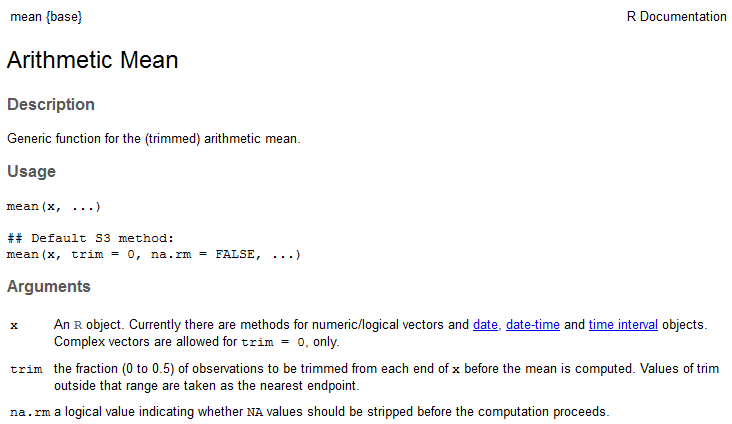
\includegraphics[width=1\linewidth]{figs/ExemploAjuda} 

}

\caption{Help screen for function mean}\label{fig:ExampleHelp}
\end{figure}

If we are looking for help for a given text and not a function name, we
can use double question marks as in \texttt{??"standard\ deviation"}.
This operation will search for the occurrence of the term in all
packages of R and it is very useful to learn how to perform a particular
task. In this case, we looked for the available functions to calculate
the standard deviation of a vector.

As a suggestion of usage, the easiest and most direct way to learn a new
function is trying out the examples in the manual. This way, you can see
which type of input objects the function expects and what type of output
it gives. Once you have it working, read the help screen to understand
if it does exactly what you expected and what are the options for its
use. If the function performs the desired procedure, you can copy and
paste the code example for your own \emph{script}, adjusting where
necessary.

Another very important source of help is the Internet itself. Sites like
\href{http://stackoverflow.com/}{stackoverflow} and specific
\emph{mailing lists}, whose content is also on the Internet, are a
valuable source of information. If you find a problem that could not be
solved by reading the standard help files, the next logical step is to
seek a solution using your error message or the description of the
problem in search engines. In many cases, your problem, no matter how
specific it is, has already occurred and has been solved by other users.
In fact, it is more surprising not to find the solution for a
programming problem on the internet, than the other way around.

\section{R Packages}\label{r-packages}

One of the greatest benefits of using R is its package collection. A
package is nothing more than a group of procedures aimed at solving a
particular computational problem. R has at its core a collaborative
philosophy. Users provide their codes for others to use. And, most
importantly, \textbf{all packages are free}. For example, consider a
case where the user is interested in accessing data about historical
inflation in the USA. He can install and use a R package that is
specifically designed for importing economic statistics for a country.

Every function in R belongs to a package. When R initializes, packages
\texttt{stats}, \texttt{graphics}, \texttt{grDevices}, \texttt{utils},
\texttt{datasets}, \texttt{methods} and \texttt{base} are loaded by
default. Almost every function we have used so far belongs to the
package \texttt{base}. R packages can be accessed and installed from
different sources. The main being \textbf{CRAN} (\emph{The Comprehensive
R Archive network}), \textbf{R-Forge} and \textbf{Github}. The quantity
and diversity of R packages increases every day. At the time of the
publication of this book, the author of this book has six packages
available on CRAN: \index{CRAN} \index{R-Forge} \index{Github}

\begin{itemize}
\item
  \href{https://CRAN.R-project.org/package=GetHFData}{GetHFData} -
  Allows direct access to high frequency financial transaction data from
  Bovespa (Brazilian Financial Exchange);
\item
  \href{https://CRAN.R-project.org/package=GetTDData}{GetTDData} -
  Enables access to prices and yields of bonds issued by the Brazilian
  government;
\item
  \href{https://CRAN.R-project.org/package=RndTexExams}{RndTexExams} -
  Enables the creation and correction of single choice exams with
  randomized content;
\item
  \href{https://CRAN.R-project.org/package=BatchGetSymbols}{BatchGetSymbols}
  - Package for easy access to daily data from Yahoo! Finance and Google
  Finance;
\item
  \href{https://CRAN.R-project.org/package=predatory}{Predatory} -
  Package to identify predatory journals based on the Beall site data;
\item
  \href{https://CRAN.R-project.org/package=pafdR}{pafdR} - Provides
  code, data and exercises for this book.
\end{itemize}

CRAN is the official repository of R and it is built by the community.
Anyone can send a package. However, there is an evaluation process to
ensure that the certain strict rules about code format are respected.
For those interested in creating and distributing packages, a clear and
easy to learn material on how to create and send packages to CRAN is
presented on the site \href{http://r-pkgs.had.co.nz/intro.html}{R
packages}. Complete rules are available on the
\href{https://cran.r-project.org/web/packages/policies.html}{CRAN
website}. The suitability of the code to CRAN standards is the
developer's responsibility. By personal experience, sending and
publishing a package on CRAN demands a significant amount of work,
especially in the first submission. After that, it becomes a lot easier.
Don't be angry if you package is rejected. My own packages were rejected
several times before entering CRAN. Listen to what the maintainers tell
you and try fixing all problems before resubmitting. If you're having
issues that you cannot solve or find a solution in the Internet, look
for help in the \href{https://www.r-project.org/mail.html}{R-packages
mailing list}. You'll be surprised at how accessible and helpful the R
community can be.

The complete list of packages available on CRAN, along with a brief
description, can be accessed at the
\href{https://cran.r-project.org/}{packages link} on the R site. A
practical way to check if there is a package that does a specific
procedure is to load the previous page and search in your \emph{browser}
for a keyword. If there is a package that does what you want, it is very
likely that the keyword is used in the description of the package.

Another important source for finding packages is
\href{https://cran.r-project.org/web/views/}{Task Views}. There you can
find the most important packages for a given area of expertise. See the
\emph{Task Views} screen in Figure \ref{fig:TaskViews}.

\begin{figure}[!htbp]

{\centering 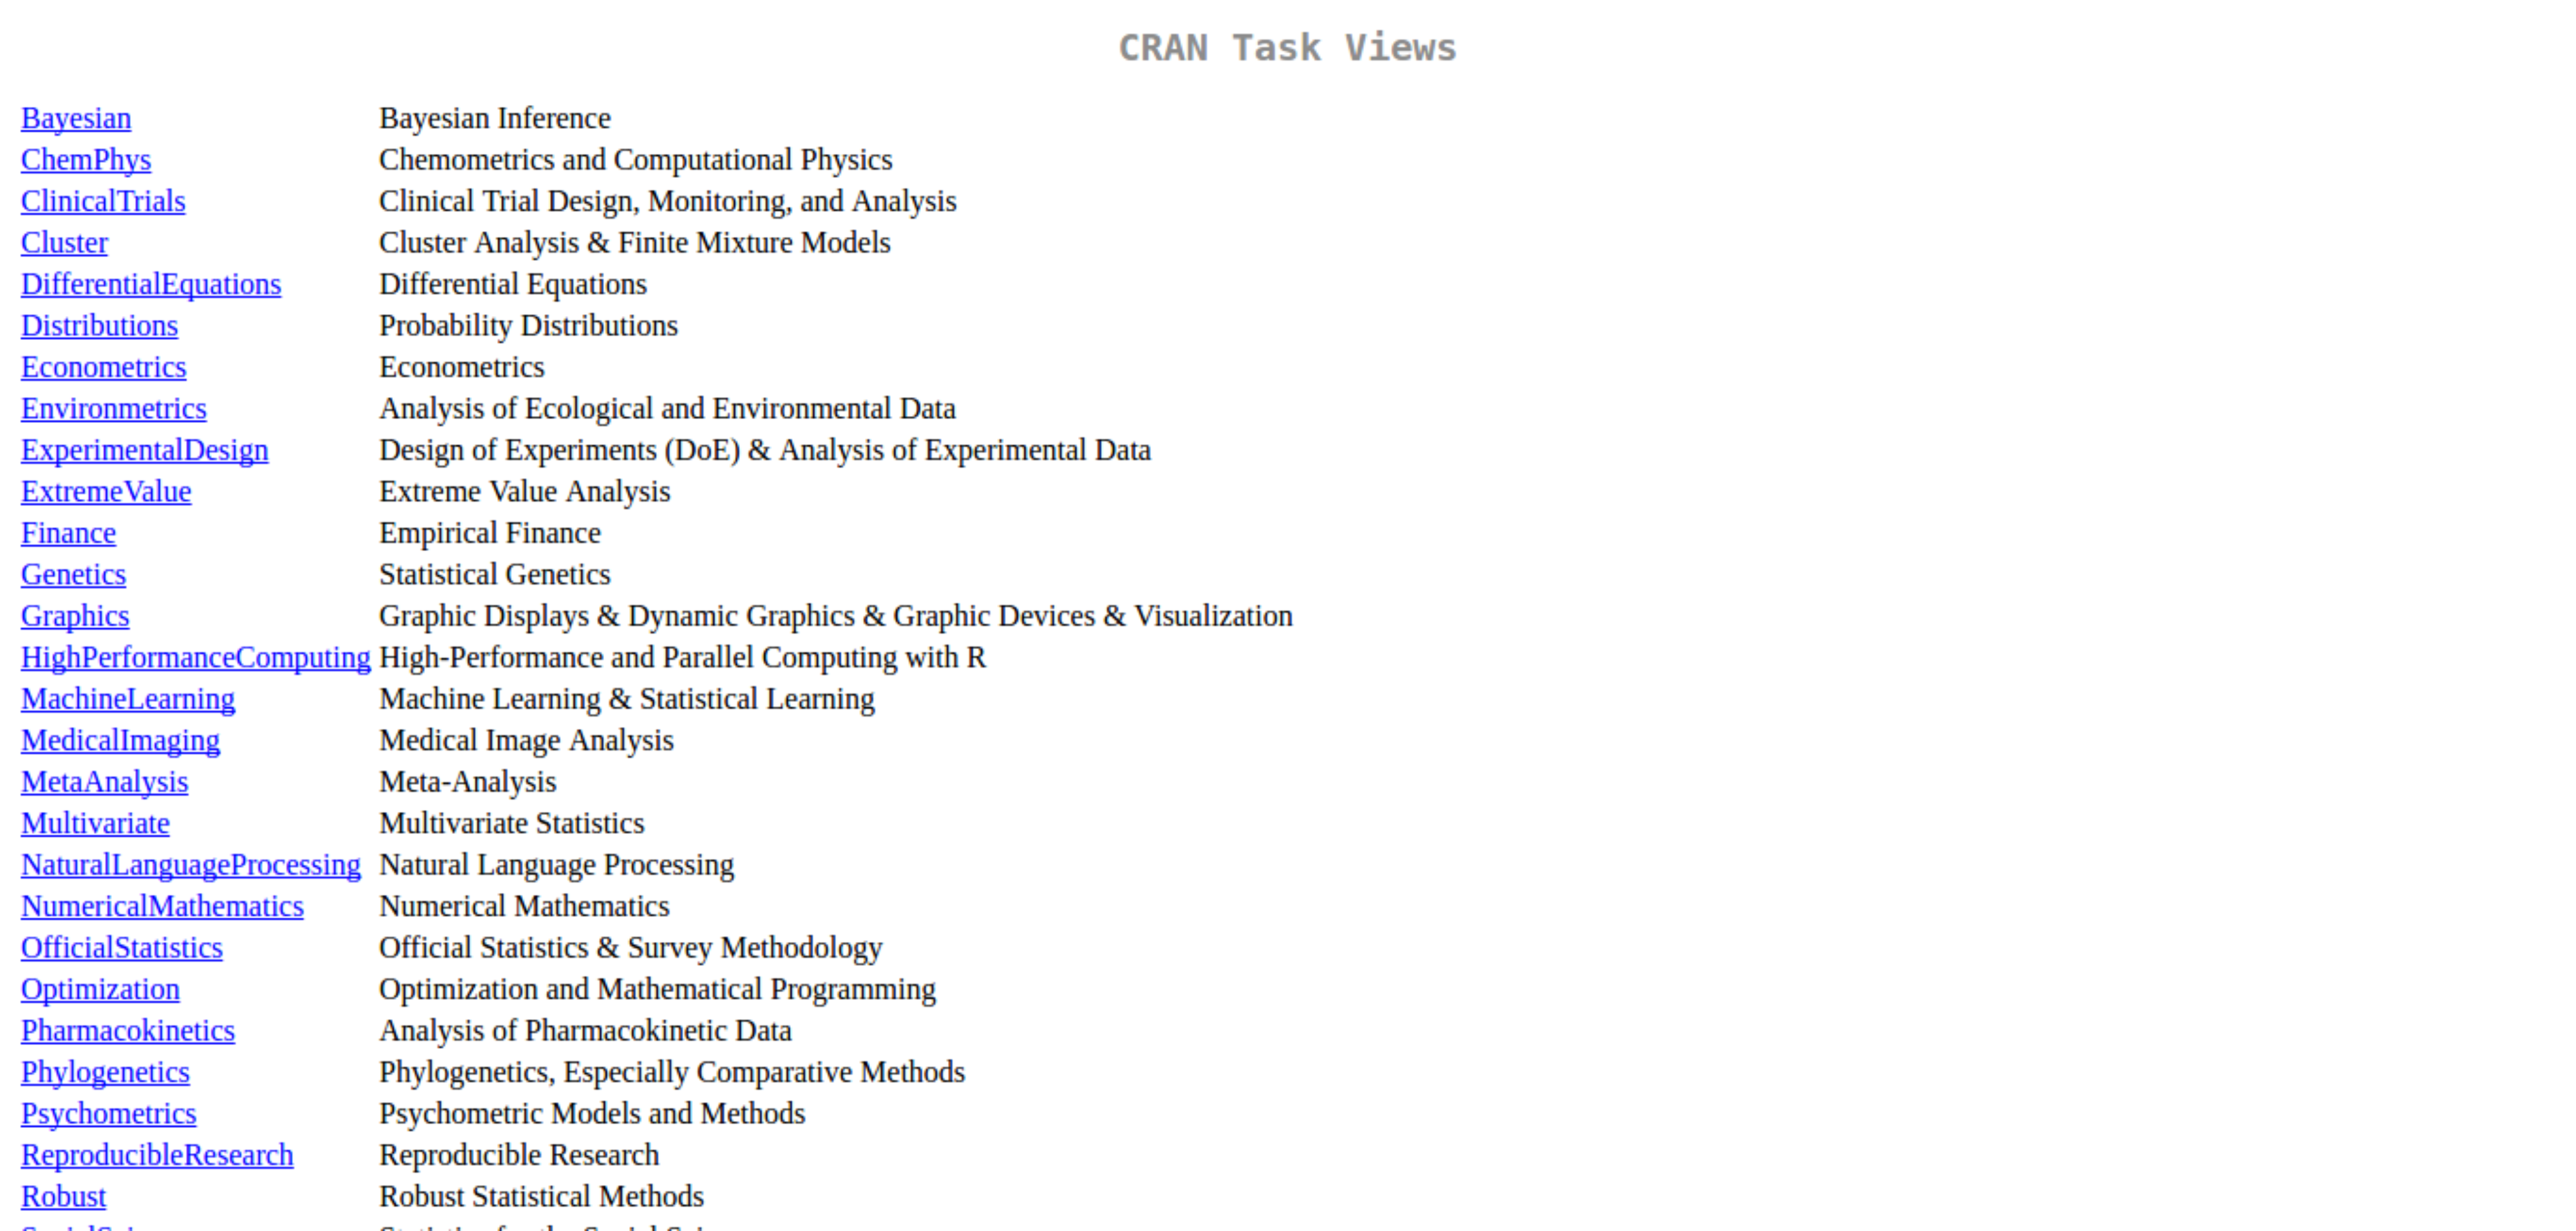
\includegraphics[width=1\linewidth]{figs/TaskViews} 

}

\caption{Task View screen}\label{fig:TaskViews}
\end{figure}

Unlike CRAN, R-Forge and Github have no restriction on the code sent to
their repository and, because of this, these repositories tend to be
chosen by developers. Responsibility in the use, however, is with the
user. In practice, it is very common for developers to maintain a
development version on Github or R-Forge and the official version in
CRAN. When the development version reaches a certain stage of maturity,
it is then sent to CRAN.

The most interesting part of this is that the packages can be accessed
and installed directly from the prompt using the internet. To find out
the current amount of packages on CRAN, type and execute the following
commands in the prompt:

\begin{Shaded}
\begin{Highlighting}[]
\CommentTok{# get matrix with available packages}
\NormalTok{df.cran.pkgs <-}\StringTok{ }\KeywordTok{available.packages}\NormalTok{()}

\CommentTok{# find the number of packages}
\NormalTok{n.cran.packages <-}\StringTok{ }\KeywordTok{nrow}\NormalTok{(df.cran.pkgs)}

\CommentTok{# print it}
\KeywordTok{print}\NormalTok{(n.cran.packages)}
\end{Highlighting}
\end{Shaded}

\begin{verbatim}
## [1] 10487
\end{verbatim}

If asked about which mirror to use, simply select the one closest to
you. Currently (2017-05-03 15:19:13), there are 10487 packages available
on the CRAN servers. We can see some details of the first three packages
in \texttt{df.cran.pkgs} with function \texttt{print} and some indexing:
\index{base!available.packages}

\begin{Shaded}
\begin{Highlighting}[]
\CommentTok{# print information about the first three packages}
\KeywordTok{print}\NormalTok{(df.cran.pkgs[}\DecValTok{1}\OperatorTok{:}\DecValTok{3}\NormalTok{, ])}
\end{Highlighting}
\end{Shaded}

\begin{verbatim}
##        Package  Version Priority
## A3     "A3"     "1.0.0" NA      
## abbyyR "abbyyR" "0.5.1" NA      
## abc    "abc"    "2.1"   NA      
##        Depends                                              
## A3     "R (>= 2.15.0), xtable, pbapply"                     
## abbyyR "R (>= 3.2.0)"                                       
## abc    "R (>= 2.10), abc.data, nnet, quantreg, MASS, locfit"
##        Imports                                  LinkingTo
## A3     NA                                       NA       
## abbyyR "httr, XML, curl, readr, plyr, progress" NA       
## abc    NA                                       NA       
##        Suggests                               Enhances
## A3     "randomForest, e1071"                  NA      
## abbyyR "testthat, rmarkdown, knitr (>= 1.11)" NA      
## abc    NA                                     NA      
##        License              License_is_FOSS
## A3     "GPL (>= 2)"         NA             
## abbyyR "MIT + file LICENSE" NA             
## abc    "GPL (>= 3)"         NA             
##        License_restricts_use OS_type Archs MD5sum
## A3     NA                    NA      NA    NA    
## abbyyR NA                    NA      NA    NA    
## abc    NA                    NA      NA    NA    
##        NeedsCompilation File
## A3     "no"             NA  
## abbyyR "no"             NA  
## abc    "no"             NA  
##        Repository                               
## A3     "https://cloud.r-project.org/src/contrib"
## abbyyR "https://cloud.r-project.org/src/contrib"
## abc    "https://cloud.r-project.org/src/contrib"
\end{verbatim}

In short, object \texttt{df.cran.pkgs} displays the names of packages,
its current version, its dependencies, along with various other
information.

You can also check the amount of locally installed packages in R with
the \texttt{installed.packages} command: \index{base!installed.packages}

\begin{Shaded}
\begin{Highlighting}[]
\CommentTok{# find number of packages currently installed}
\NormalTok{n.local.packages <-}\StringTok{ }\KeywordTok{nrow}\NormalTok{(}\KeywordTok{installed.packages}\NormalTok{())}

\CommentTok{# print it }
\KeywordTok{print}\NormalTok{(n.local.packages)}
\end{Highlighting}
\end{Shaded}

\begin{verbatim}
## [1] 364
\end{verbatim}

In this case, the computer on which the book was written has 364
packages currently installed. This value is probably different from
yours. Give it a try!

\subsection{Installing Packages from
CRAN}\label{installing-packages-from-cran}

To install a package, simply use the command \texttt{install.packages}.
You only need to do it once for each new package. As an example, we will
install a package called \texttt{quantmod} that will be used in future
chapters. \index{base!install.packages}

\begin{Shaded}
\begin{Highlighting}[]
\CommentTok{# install package quantmod}
\KeywordTok{install.packages}\NormalTok{(}\StringTok{"quantmod"}\NormalTok{)}
\end{Highlighting}
\end{Shaded}

That's it! After executing this simple command, package
\texttt{quantmod} and all of its dependencies will be installed and the
functions related to the package will be ready for use once the package
is loaded in a script. Note that we defined the package name in the
installation as if it were text with the use of quotation marks
(\texttt{"\ "}). If the installed package is dependent on another
package, R detects this dependency and automatically installs the
missing packages. Thus, all the requirements for using the installed
package will already be satisfied and everything will work perfectly. It
is possible, however, that a package has an external dependency. As an
example, package \texttt{RndTexExams} depends on the existence of a
LaTeX installation. These cases are usually announced in the description
of the package and an error informs that a requirement is missing.
External dependencies for R packages are not common, but they do happen.

\subsection{Installing Packages from
Github}\label{installing-packages-from-github}

To install a package hosted in Github, you must install the
\emph{devtools} package, available on CRAN: \index{devtools}

\begin{Shaded}
\begin{Highlighting}[]
\CommentTok{# install devtools}
\KeywordTok{install.packages}\NormalTok{(}\StringTok{'devtools'}\NormalTok{)}
\end{Highlighting}
\end{Shaded}

After that, load up the package \texttt{devtools} and use the function
\texttt{install\_github} to install a package directly from Github. In
the following example, we install the development version of the package
\texttt{ggplot2}, whose official version is also available at CRAN:
\index{devtools!install\_github}

\begin{Shaded}
\begin{Highlighting}[]
\CommentTok{# load up devtools}
\KeywordTok{library}\NormalTok{(devtools)}

\CommentTok{# install ggplot2 from github}
\KeywordTok{install_github}\NormalTok{(}\StringTok{"hadley/ggplot2"}\NormalTok{)}
\end{Highlighting}
\end{Shaded}

Note that the username of the developer is also included. In this case,
the \emph{hadley} name belongs to the developer of \texttt{ggplot2},
Hadley Wickham. Throughout the book, you will notice that this name
appears several times. Hadley is a prolific and competent developer of
several R packages and currently works for RStudio.

\subsection{Loading Packages}\label{loading-packages}

Within a script, use function \texttt{library} to load a package, as in
the following example. \index{base!library}

\begin{Shaded}
\begin{Highlighting}[]
\CommentTok{# load package quantmod}
\KeywordTok{library}\NormalTok{(quantmod)}
\end{Highlighting}
\end{Shaded}

After running this command, all functions of the package will be
available to the user. In this case, it is not necessary to use
\texttt{"\ "} to load the package. If the package you want to use is not
available, R will throw an error message. See an example next, where we
try to load a non-existing package called \texttt{unicorn}.

\begin{Shaded}
\begin{Highlighting}[]
\KeywordTok{library}\NormalTok{(unicorn)}
\end{Highlighting}
\end{Shaded}

\begin{verbatim}
## Error in library(unicorn): there is no package called 'unicorn'
\end{verbatim}

Remember this error message. It will appear every time a package is not
found. If you got the same message when running code from this book, you
need to check what are the required packages of the example and install
them using \texttt{install.packages}, as in
\texttt{install.packages(\textquotesingle{}unicorn\textquotesingle{})}.

If you use a specific package function and do not want to load all
functions from the package, you can do it through the special symbol
\texttt{::}, as in the following example. \index{base!::}

\begin{Shaded}
\begin{Highlighting}[]
\CommentTok{# example of using a function without loading package}
\NormalTok{fortunes}\OperatorTok{::}\KeywordTok{fortune}\NormalTok{(}\DecValTok{10}\NormalTok{)}
\end{Highlighting}
\end{Shaded}

\begin{verbatim}
## 
## Overall, SAS is about 11 years behind R and S-Plus in
## statistical capabilities (last year it was about 10 years
## behind) in my estimation.
##    -- Frank Harrell (SAS User, 1969-1991)
##       R-help (September 2003)
\end{verbatim}

In this case, we use the function \texttt{fortune} from the package
\texttt{fortunes}, which shows on screen a potentially funny phrase
chosen from the R mailing list. For our example, we selected message
number 10. One interesting use of the package \texttt{fortune} is to
display a different message every time R starts. As mentioned before,
you can find many tutorials on how to achieve this effect by searching
on the web for ``customizing R startup''.

Another way of loading a package is using the \texttt{require} function.
A call to \texttt{require} has a different behaviour than a call to
\texttt{library}. When using \texttt{library}, if the package is not
found in the local libraries, it returns an error. This means that the
script stops and no further code is evaluated. As for \texttt{require},
if a package is not found, it returns an object with value
\texttt{FALSE} and the rest of the code is evaluated. So, in order to
avoid code being executed without its explicit dependencies, it is
advised to always use \texttt{library} for loading package in scripts.
\index{base!required}

The use of \texttt{require} is left for loading up packages inside of
functions. If you create a custom function that requires procedures from
a particular package, you must load the package within the scope of the
function. For example, see the following code, where we create a new
function called \texttt{my.fct} that depends on the package
\texttt{quantmod}:

\begin{Shaded}
\begin{Highlighting}[]
\NormalTok{my.fct <-}\StringTok{ }\ControlFlowTok{function}\NormalTok{(x)\{}
    \KeywordTok{require}\NormalTok{(quantmod)}
    
\NormalTok{    df <-}\StringTok{ }\KeywordTok{getSymbols}\NormalTok{(x, }\DataTypeTok{auto.assign =}\NormalTok{ F)}
    \KeywordTok{return}\NormalTok{(df)}
\NormalTok{\}}
\end{Highlighting}
\end{Shaded}

In this case, the first time that \texttt{my.fct} is called, it loads up
the package \texttt{quantmod} and all of its functions. Using
\texttt{require} inside a function is good programming policy because
the function becomes self contained, making it easier to use it in the
future. This was the first time where the complete definition of a
function in R is presented. Do not worry about it now. We will explain
it further in chapter \ref{programming}.

\subsection{Upgrading Packages}\label{upgrading-packages}

Over time, it is natural that the packages available on CRAN are
upgraded to accommodate new features, correct bugs and adapt to changes.
Thus, it is recommended that users update their installed packages to a
new version over the internet. In R, this procedure is quite easy. A
direct way of upgrading packages is to click the button \emph{update}
located in the package panel, lower right corner of RStudio, as shown in
Figure \ref{fig:RStudio-update}.

\begin{figure}[!htbp]

{\centering 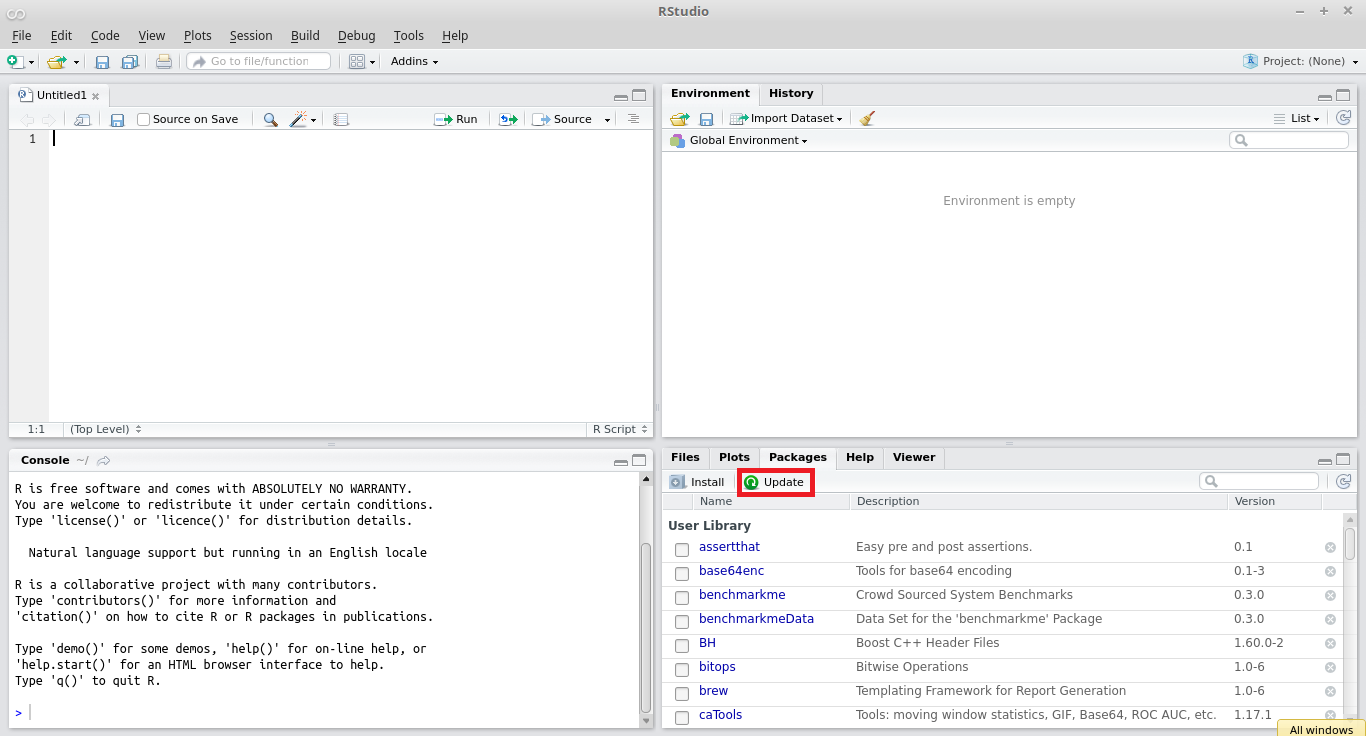
\includegraphics[width=1\linewidth]{figs/RStudio_update} 

}

\caption{Updating R packages}\label{fig:RStudio-update}
\end{figure}

The user can also update packages through the prompt. Simply type
command \texttt{update.packages()} and hit \emph{enter}, as shown below.
\index{base!update.packages}

\begin{Shaded}
\begin{Highlighting}[]
\CommentTok{# update all installed packages}
\KeywordTok{update.packages}\NormalTok{()}
\end{Highlighting}
\end{Shaded}

The command \texttt{update.packages} compares the version of the
installed packages with the versions available in CRAN. If it finds any
difference, the new versions are downloaded and installed. After running
the command, all packages will be synchronized with the versions
available in CRAN.

\section{\texorpdfstring{Using Code Completion with
\emph{tab}}{Using Code Completion with tab}}\label{using-code-completion-with-tab}

A very useful feature of RStudio is \emph{code completion}. This is an
editing tool that facilitates the search of names for objects, packages,
function arguments and files. Its usage is very simple. After you type
any first character, just press the \emph{tab} (left side of keyboard,
above \emph{capslock}) and a number of options will appear. See Figure
\ref{fig:autocomplete} where, after entering the \emph{f} letter and
pressing \emph{tab}, a window appears with a list of object names that
begins with that letter. \index{code completion}

\begin{figure}[!htbp]

{\centering 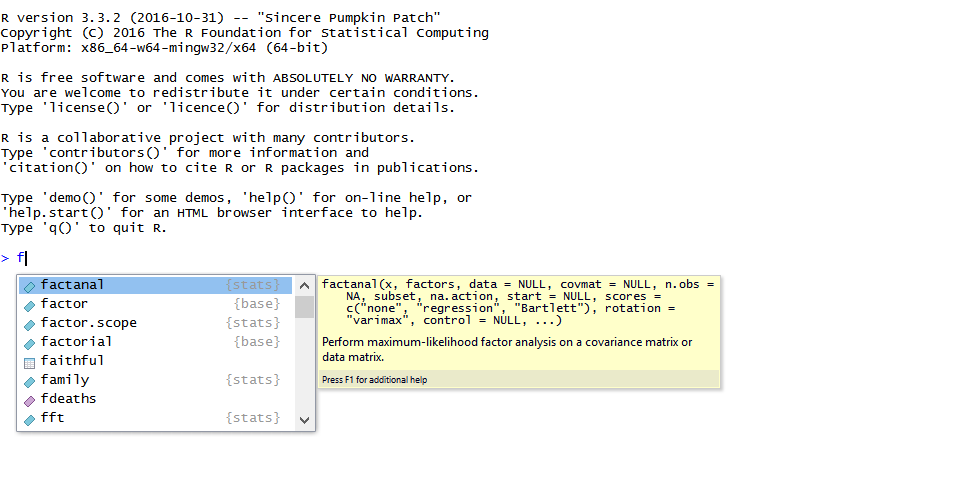
\includegraphics[width=1\linewidth]{figs/autocomplete} 

}

\caption{Usage of autocomplete for object name}\label{fig:autocomplete}
\end{figure}

This also works for packages. To check it, type \texttt{library(r)} in
the prompt or editor, place the cursor in between the parentheses and
press \emph{tab}. The result should look something like Figure
\ref{fig:autocomplete-packages}, shown next.

\begin{figure}[!htbp]

{\centering 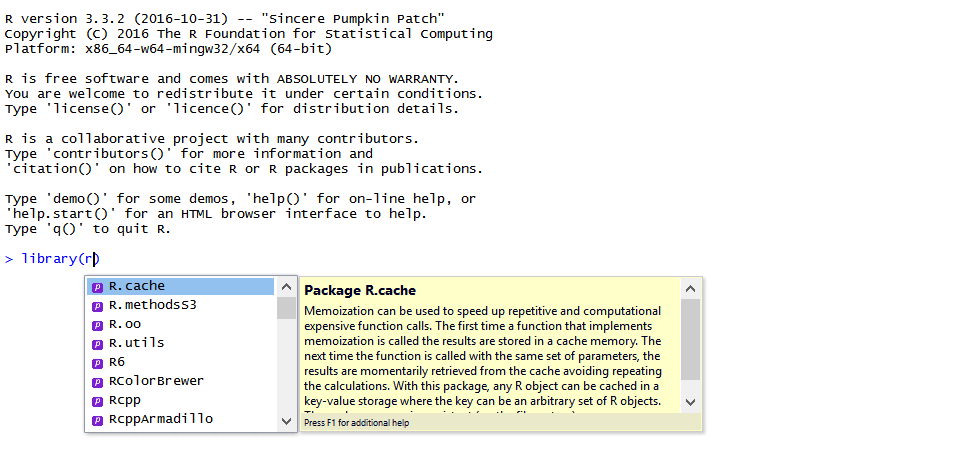
\includegraphics[width=1\linewidth]{figs/autocomplete_pacotes} 

}

\caption{Usage of autocomplete for packages}\label{fig:autocomplete-packages}
\end{figure}

Note that a description of the package or object is also offered by the
code completion tool. This greatly facilitates the day to day work as
the memorization of package names and R objects is not an easy task. The
use of the \emph{tab} decreases the time to look up names, also avoiding
possible coding errors.

The use of this tool becomes even more beneficial when objects and
functions are named with some sort of pattern. In the rest of the book,
you will notice that objects tend to be named with the prefix
\emph{my.}, as \emph{my.x}, \emph{my.num}. Using this naming rule (or
any other) facilitates the lookup for names of objects created by the
user. You can just type \emph{my.}, press \emph{tab}, and a list of all
objects previously created by the user will appear.

You can also find files and folders on your computer using \emph{tab}.
To try it, write the command \texttt{my.file\ \textless{}-\ ""} in the
prompt or a script, point the cursor to the middle of the quotes and
press the \emph{tab} key. A screen with the files and folders from the
current working directory should appear, as shown in Figure
\ref{fig:autocomplete-files}. You can use the keyboard arrow keys to
navigate.

\begin{figure}[!htbp]

{\centering 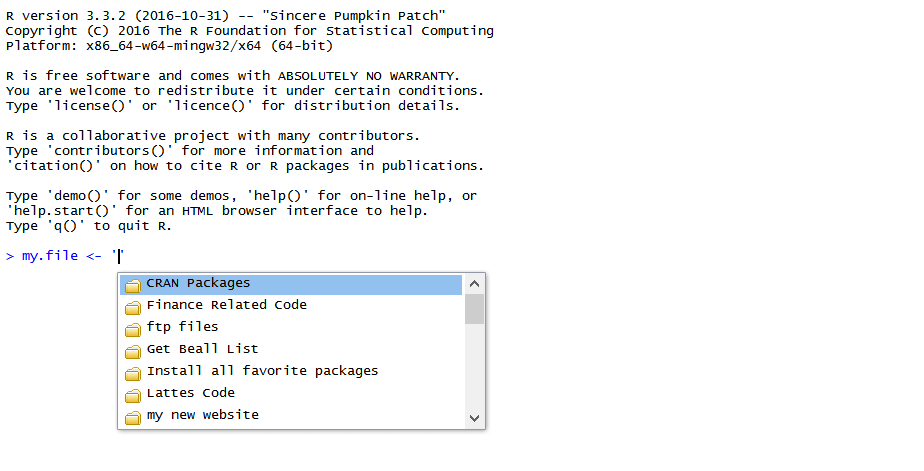
\includegraphics[width=1\linewidth]{figs/autocomplete_arquivos} 

}

\caption{Usage of autocomplete for files and folders}\label{fig:autocomplete-files}
\end{figure}

The use of autocomplete is also possible for finding the name and
description of function arguments. To try it out, write \texttt{cat()}
and place the mouse cursor inside the parentheses. After that, press
\emph{tab}. The result should be similar to Figure
\ref{fig:autocomplete-args}.

\begin{figure}[!htbp]

{\centering 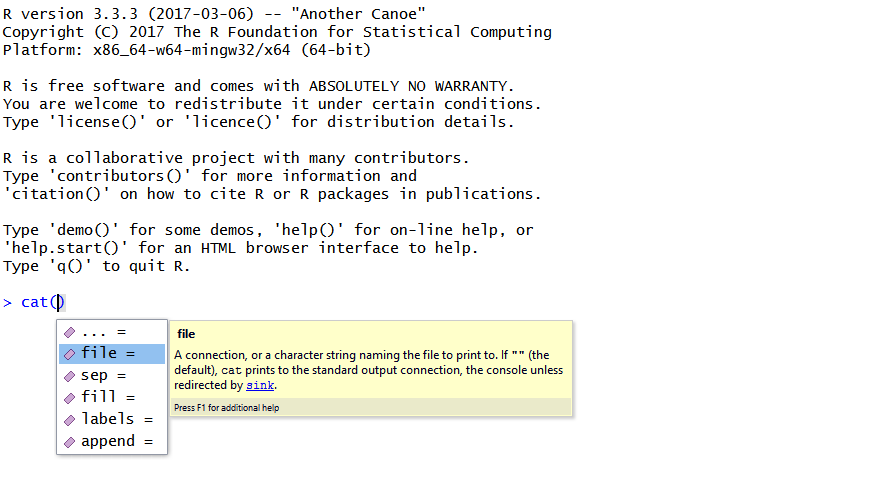
\includegraphics[width=0.75\linewidth]{figs/autocomplete_args} 

}

\caption{Usage of autocomplete for function arguments}\label{fig:autocomplete-args}
\end{figure}

By using \emph{tab} inside of a function, we have the names of all
arguments and their description. This is the same information found in
the help files.

Summing up, using code completion will make you more productive. You'll
find names of files, objects, arguments and packages much faster. Use it
whenever possible.

\section{Interacting with Files and the Operating
System}\label{interacting-with-files-and-the-operating-system}

In many data analysis situations, it will be necessary to interact with
files in the computer, either by creating new folders, decompressing and
compressing files, listing and removing files from the hard drive of the
computer or any other type of operation. In most cases, R will interact
with files containing data.

\subsection{Listing Files and Folders}\label{listing-files-and-folders}

To list files from your computer, use function \texttt{list.files},
where the \texttt{path} argument sets the directory to list the files
from. For the compilation of the book, I've created a directory called
\emph{data}. This folder contains all the data needed to recreate the
book's examples. You can check the files in the subfolder \texttt{data}
with the following code: \index{base!list.files}

\begin{Shaded}
\begin{Highlighting}[]
\CommentTok{# list files in data folder}
\NormalTok{my.f <-}\StringTok{ }\KeywordTok{list.files}\NormalTok{(}\DataTypeTok{path =} \StringTok{"data"}\NormalTok{, }\DataTypeTok{full.names =} \OtherTok{TRUE}\NormalTok{)}
\KeywordTok{print}\NormalTok{(my.f)}
\end{Highlighting}
\end{Shaded}

\begin{verbatim}
##  [1] "data/AdjustedPrices-InternacionalIndices.RDATA"
##  [2] "data/BovStocks_2011-12-01_2016-11-29.csv"      
##  [3] "data/BovStocks_2011-12-01_2016-11-29.RData"    
##  [4] "data/example_gethfdata.RDATA"                  
##  [5] "data/FileWithLatinChar.txt"                    
##  [6] "data/grunfeld.csv"                             
##  [7] "data/HFData.csv"                               
##  [8] "data/HFData_6_Assets_15 min.RData"             
##  [9] "data/MktIndices_and_Symbols.csv"               
## [10] "data/MySQLiteDatabase.SQLITE"                  
## [11] "data/SP500-Excel.xlsx"                         
## [12] "data/SP500-Stocks-WithRet.RData"               
## [13] "data/SP500-Stocks_long.csv"                    
## [14] "data/SP500-Stocks_wide.csv"                    
## [15] "data/SP500.csv"                                
## [16] "data/SP500_2011-11-13_2016-11-11.csv"          
## [17] "data/TDData.csv"                               
## [18] "data/temp.csv"                                 
## [19] "data/temp.RData"                               
## [20] "data/temp.txt"                                 
## [21] "data/temp.xlsx"                                
## [22] "data/temp_xts.RData"
\end{verbatim}

Note that in this directory, there are several files with different
extensions. These files contain data that will be used in future
chapters. When using \texttt{list.files}, it is recommended to set input
\texttt{full.names} as \texttt{TRUE}. This option makes sure that the
names returned by the function contains the full path of the found
files. This facilitates further manipulation, such as reading and
importing information from data files. It is worth noting that you can
also list the files recursively, that is, list all files from all
subfolders contained in the original address. To check it, try using the
following code in your computer:

\begin{Shaded}
\begin{Highlighting}[]
\CommentTok{# list all files for all subfolders (IT MAY TAKE SOME TIME...)}
\KeywordTok{list.files}\NormalTok{(}\DataTypeTok{path =} \KeywordTok{getwd}\NormalTok{(), }\DataTypeTok{recursive =}\NormalTok{ T, }\DataTypeTok{full.names =} \OtherTok{TRUE}\NormalTok{)}
\end{Highlighting}
\end{Shaded}

The previous command will list all files in the current folder and
subfolders. Depending on the current working directory, it may take some
time to run it all. If you executed it, be patient or just cancel it
pressing \texttt{esc}.

To list folders (directories) on your computer, use the command
\texttt{list.dirs}. See below. \index{base!list.dirs}

\begin{Shaded}
\begin{Highlighting}[]
\CommentTok{# store names of directories}
\NormalTok{my.dirs <-}\StringTok{ }\KeywordTok{list.dirs}\NormalTok{(}\DataTypeTok{recursive =}\NormalTok{ F)}

\CommentTok{# print it}
\KeywordTok{print}\NormalTok{(my.dirs)}
\end{Highlighting}
\end{Shaded}

\begin{verbatim}
##  [1] "./.Rproj.user"              
##  [2] "./_bookdown_files"          
##  [3] "./data"                     
##  [4] "./docs"                     
##  [5] "./eqs"                      
##  [6] "./fig_ggplot"               
##  [7] "./figs"                     
##  [8] "./ftp files"                
##  [9] "./latex_files"              
## [10] "./many_datafiles"           
## [11] "./ProcAnFinDataR_ed_1_cache"
## [12] "./ProcAnFinDataR_ed_1_files"
## [13] "./Removed chapters"         
## [14] "./Scripts"                  
## [15] "./tabs"
\end{verbatim}

The command \texttt{list.dirs(recursive\ =\ F)} listed all directories
of the current path without recursion. The output shows the directories
that I have used to write this book. It includes the output directory of
the book ( \texttt{./\_book}), the directory with the data
(\texttt{./data}), among others. In this same directory, you can find
the chapters of the book, organized by files and based on the
\emph{RMarkdown} language (\texttt{.Rmd} file extension). To list only
files with the extension \texttt{.Rmd}, we can use the \texttt{pattern}
input in function \texttt{list.files} as follows:

\begin{Shaded}
\begin{Highlighting}[]
\CommentTok{# list all files with extension .Rmd}
\KeywordTok{list.files}\NormalTok{(}\DataTypeTok{pattern =} \StringTok{"*.Rmd"}\NormalTok{)}
\end{Highlighting}
\end{Shaded}

\begin{verbatim}
##  [1] "_Welcome.Rmd"                               
##  [2] "00-Preface.Rmd"                             
##  [3] "01-Introduction.Rmd"                        
##  [4] "02-BasicOperations.Rmd"                     
##  [5] "03-BasicObjects.Rmd"                        
##  [6] "04-DataStructureObjects.Rmd"                
##  [7] "05-Financial-data-and-common-operations.Rmd"
##  [8] "06-ImportingExportingLocal.Rmd"             
##  [9] "07-ImportingInternet.Rmd"                   
## [10] "08-Figures.Rmd"                             
## [11] "09-Programming.Rmd"                         
## [12] "10-Models.Rmd"                              
## [13] "11-ResearchScripts.Rmd"                     
## [14] "12-references.Rmd"                          
## [15] "index.Rmd"                                  
## [16] "ProcAnFinDataR_ed_1.Rmd"
\end{verbatim}

The files presented above contain all the contents of this book,
including this specific paragraph, located in file
\texttt{02-BasicOperations.Rmd}!

\hypertarget{BasicObjects}{\chapter{Basic Object
Classes}\label{BasicObjects}}

\textbf{In R, everything is an object}. Previously, we executed commands
in the prompt, and it resulted in creating objects in our environment.
Each type of object will have several different properties. A
\texttt{numeric} object may interact with other \texttt{numeric} objects
in operations such as multiplication, division, and addition. This is
not true for objects belonging to the class \texttt{character}, where
mathematical properties are not valid or intuitive - it does not make
sense to add a numeric value to a text or to divide a text for other
text.

But, the \texttt{character} class has other properties, such as allowing
the user to look for a specific text within a larger text, splitting
parts of a text, and replacing specific characters, among many other
possibilities. \textbf{One of the most important aspects of working with
R is learning the functionalities of the object classes}.

An important distinction here is the difference between basic and data
structure type of classes. The basic classes are the primary elements in
data representation. It includes numerical values, logical objects,
characters (text), factors, dates, among many other cases. The basic
classes are stored in more complex data structures that aggregate the
information and facilitate the work. Imagine conducting a study based on
closing prices of 500 stocks that belong to the SP500 market index. If
we create a numeric vector of prices for each stock, we would have
several \emph{500} objects to handle in our environment! Although you
can work this way, the resulting code would be disorganized, difficult
to understand, and subject to several errors.
\index{basic object classes}

A simpler way to organize our data is to create an object with the name
\texttt{SP500.data} and allocate the prices of all stocks there. All
necessary information to perform our research would be available in that
object, making it easier to import and export data. These objects that
store other basic class objects are the data structure type. This
classification includes lists, matrices, and data frames. In this
section, we will address the most basic types of objects in R. The data
structure types will be presented in the next chapter.

\section{\texorpdfstring{\texttt{Numeric}
Objects}{Numeric Objects}}\label{numeric-objects}

Objects of type \texttt{numeric} represent one or more quantities and
are one of the most used objects in data research, for example, the
price of a stock at a given date, the trading volume of a financial
contract on any given day, the net profit of a company at the end of the
year, among many other possibilities. Generally, numerical vectors are
imported from an existing database. However, you can also register them
from the editor. \index{numeric}

\subsection{\texorpdfstring{Creating and Manipulating \texttt{numeric}
Objects}{Creating and Manipulating numeric Objects}}\label{creating-and-manipulating-numeric-objects}

The creation and manipulation of \texttt{numeric} objects is easy. As
expected, we can use the common symbols of mathematical operations, such
as sum (\texttt{+}), difference (\texttt{-}), division (\texttt{/}) and
multiplication (\texttt{*}). When working with \texttt{numeric} vectors,
all mathematical operations are carried out using an \textbf{element by
element} orientation. See the next example, where we create two vectors
and perform various operations.

\begin{Shaded}
\begin{Highlighting}[]
\CommentTok{# create numeric vectors}
\NormalTok{x <-}\StringTok{ }\DecValTok{1}\OperatorTok{:}\DecValTok{5}
\NormalTok{y <-}\StringTok{ }\DecValTok{2}\OperatorTok{:}\DecValTok{6}

\CommentTok{# print sum}
\KeywordTok{print}\NormalTok{(x}\OperatorTok{+}\NormalTok{y)}
\end{Highlighting}
\end{Shaded}

\begin{verbatim}
## [1]  3  5  7  9 11
\end{verbatim}

\begin{Shaded}
\begin{Highlighting}[]
\CommentTok{# print multiplication}
\KeywordTok{print}\NormalTok{(x}\OperatorTok{*}\NormalTok{y)}
\end{Highlighting}
\end{Shaded}

\begin{verbatim}
## [1]  2  6 12 20 30
\end{verbatim}

\begin{Shaded}
\begin{Highlighting}[]
\CommentTok{# print division}
\KeywordTok{print}\NormalTok{(x}\OperatorTok{/}\NormalTok{y)}
\end{Highlighting}
\end{Shaded}

\begin{verbatim}
## [1] 0.5000000 0.6666667 0.7500000 0.8000000 0.8333333
\end{verbatim}

\begin{Shaded}
\begin{Highlighting}[]
\CommentTok{# print exponentiation}
\KeywordTok{print}\NormalTok{(x}\OperatorTok{^}\NormalTok{y)}
\end{Highlighting}
\end{Shaded}

\begin{verbatim}
## [1]     1     8    81  1024 15625
\end{verbatim}

A difference between R and other programming languages is that
operations between vectors of different sizes are accepted. We can add a
\texttt{numeric} vector with four elements with the other containing
only two elements. Whenever that happens, R calls for the
\textbf{recycling rule}. It states, if two different sized vectors are
interacting, the smaller vector is repeated as often as necessary to
obtain the same number of elements as the larger vector. See the
following example: \index{recycling rule}

\begin{Shaded}
\begin{Highlighting}[]
\CommentTok{# set x with 4 elements and y with 2}
\NormalTok{x <-}\StringTok{ }\DecValTok{1}\OperatorTok{:}\DecValTok{4}
\NormalTok{y <-}\StringTok{ }\DecValTok{2}\OperatorTok{:}\DecValTok{1}

\CommentTok{# print multiplication}
\KeywordTok{print}\NormalTok{(x }\OperatorTok{+}\StringTok{ }\NormalTok{y)}
\end{Highlighting}
\end{Shaded}

\begin{verbatim}
## [1] 3 3 5 5
\end{verbatim}

Here, the result of \texttt{x\ +\ y} is equivalent to
\texttt{1:4\ +\ c(2,\ 1,\ 2,\ 1)}. If you try to operate with vectors in
which the length of the largest vector is not a multiple of the length
of the smaller, R performs the same recycling procedure, but also sends
a \texttt{warning} message to inform the user that the recycling
procedure was not perfectly executed. See next.

\begin{Shaded}
\begin{Highlighting}[]
\CommentTok{# set x = 4 elements and y with 3}
\NormalTok{x <-}\StringTok{ }\KeywordTok{c}\NormalTok{(}\DecValTok{1}\NormalTok{, }\DecValTok{2}\NormalTok{, }\DecValTok{3}\NormalTok{, }\DecValTok{4}\NormalTok{)}
\NormalTok{y <-}\StringTok{ }\KeywordTok{c}\NormalTok{(}\DecValTok{1}\NormalTok{, }\DecValTok{2}\NormalTok{, }\DecValTok{3}\NormalTok{)}

\CommentTok{# print sum (recycling rule)}
\KeywordTok{print}\NormalTok{(x }\OperatorTok{+}\NormalTok{y)}
\end{Highlighting}
\end{Shaded}

\begin{verbatim}
## Warning in x + y: longer object length is not a multiple of
## shorter object length
\end{verbatim}

\begin{verbatim}
## [1] 2 4 6 5
\end{verbatim}

The first three elements of \texttt{x} were summed to the first three
elements of \texttt{y}. The fourth element of \texttt{x} was summed to
the first element of \texttt{y}. Since there was no fourth element in
\texttt{y}, R cycled through the values of the vector, restarting with
the first element.

One great thing about R is that elements of a \texttt{numeric} vector
can be named. See an example next, where we create a vector with several
named items.

\begin{Shaded}
\begin{Highlighting}[]
\CommentTok{# create named vector}
\NormalTok{x <-}\StringTok{ }\KeywordTok{c}\NormalTok{(}\DataTypeTok{item1 =} \DecValTok{10}\NormalTok{, }\DataTypeTok{item2 =} \DecValTok{14}\NormalTok{, }\DataTypeTok{item3 =} \DecValTok{9}\NormalTok{, }\DataTypeTok{item4 =} \DecValTok{2}\NormalTok{)}

\CommentTok{# print it}
\KeywordTok{print}\NormalTok{(x)}
\end{Highlighting}
\end{Shaded}

\begin{verbatim}
## item1 item2 item3 item4 
##    10    14     9     2
\end{verbatim}

Notice how we used symbol \texttt{=} to set the names of the elements
inside of function \texttt{c} (combine). As mentioned, the equality
symbol is usually used to define arguments of a function call. To name
elements of a \texttt{numeric} vector after creating it, we can use the
\texttt{names} function. See below: \index{base!names}

\begin{Shaded}
\begin{Highlighting}[]
\CommentTok{# create unnamed vector}
\NormalTok{x <-}\StringTok{ }\KeywordTok{c}\NormalTok{(}\DecValTok{10}\NormalTok{, }\DecValTok{14}\NormalTok{, }\DecValTok{9}\NormalTok{, }\DecValTok{2}\NormalTok{)}

\CommentTok{# set names of elements}
\KeywordTok{names}\NormalTok{(x) <-}\StringTok{ }\KeywordTok{c}\NormalTok{(}\StringTok{'item1'}\NormalTok{, }\StringTok{'item2'}\NormalTok{, }\StringTok{'item3'}\NormalTok{, }\StringTok{'item4'}\NormalTok{)}

\CommentTok{# print it}
\KeywordTok{print}\NormalTok{(x)}
\end{Highlighting}
\end{Shaded}

\begin{verbatim}
## item1 item2 item3 item4 
##    10    14     9     2
\end{verbatim}

Notice how the use of function \texttt{names} works differently from the
previous examples. Here, we use the function on the left side of
\texttt{\textless{}-} and not on the right. The intuition of assigning a
value using \texttt{\textless{}-} still holds as we are registering an
attribute of the object, the name of its elements. This notation may
seem strange, at first, but it gets familiar with time and use.

Empty \texttt{numeric} vectors can also be created. Sometimes, you need
to set an empty vector to be filled with values later. For that, use the
\texttt{numeric} function: \index{base!numeric}

\begin{Shaded}
\begin{Highlighting}[]
\CommentTok{# create empty numeric vector of length 10}
\NormalTok{my.x <-}\StringTok{ }\KeywordTok{numeric}\NormalTok{(}\DataTypeTok{length =} \DecValTok{10}\NormalTok{)}

\CommentTok{# print it}
\KeywordTok{print}\NormalTok{(my.x)}
\end{Highlighting}
\end{Shaded}

\begin{verbatim}
##  [1] 0 0 0 0 0 0 0 0 0 0
\end{verbatim}

As you can see, when using \texttt{numeric(length\ =\ 10)}, all values
are set to zero.

\subsection{\texorpdfstring{Creating a \texttt{numeric}
Sequence}{Creating a numeric Sequence}}\label{creating-a-numeric-sequence}

In R, you have two ways to create a sequence of numerical values. The
first, used extensively in the previous examples, is with operator
\texttt{:}, as in \texttt{my.seq\ \textless{}-\ 1:10}. This method is
practical, because the notation is clear and direct. \index{:}

However, using operator \texttt{:} limits the possibilities of the
sequences we can create. It only creates sequences where the difference
between adjacent elements is +1 or -1. A more powerful version for the
creation of sequences is the use of function \texttt{seq}. With it, you
can set the intervals between each value with argument \texttt{by}. See
an example next: \index{base!seq}

\begin{Shaded}
\begin{Highlighting}[]
\CommentTok{# create sequence with seq}
\NormalTok{my.seq <-}\StringTok{ }\KeywordTok{seq}\NormalTok{(}\DataTypeTok{from =} \OperatorTok{-}\DecValTok{10}\NormalTok{, }\DataTypeTok{to =} \DecValTok{10}\NormalTok{, }\DataTypeTok{by =} \DecValTok{2}\NormalTok{)}

\CommentTok{# print it}
\KeywordTok{print}\NormalTok{(my.seq)}
\end{Highlighting}
\end{Shaded}

\begin{verbatim}
##  [1] -10  -8  -6  -4  -2   0   2   4   6   8  10
\end{verbatim}

Another interesting feature of function \texttt{seq} is the possibility
of creating equally spaced vectors with an initial value, a final value,
and the desired number of elements. This is accomplished using option
\texttt{length.out}. In the following code, we create an array from 0 to
10 with exactly 20 elements:

\begin{Shaded}
\begin{Highlighting}[]
\CommentTok{# create sequence with defined number of elements}
\NormalTok{my.seq <-}\StringTok{ }\KeywordTok{seq}\NormalTok{(}\DataTypeTok{from =} \DecValTok{0}\NormalTok{, }\DataTypeTok{to =} \DecValTok{10}\NormalTok{, }\DataTypeTok{length.out =} \DecValTok{20}\NormalTok{)}

\CommentTok{# print it}
\KeywordTok{print}\NormalTok{(my.seq)}
\end{Highlighting}
\end{Shaded}

\begin{verbatim}
##  [1]  0.0000000  0.5263158  1.0526316  1.5789474  2.1052632
##  [6]  2.6315789  3.1578947  3.6842105  4.2105263  4.7368421
## [11]  5.2631579  5.7894737  6.3157895  6.8421053  7.3684211
## [16]  7.8947368  8.4210526  8.9473684  9.4736842 10.0000000
\end{verbatim}

Observe how the final size of \texttt{my.seq} is exactly 20, where R
automatically calculates and sets the difference of 0.5263158 between
the adjacent elements.

\subsection{Creating Vectors with Repeated
Elements}\label{creating-vectors-with-repeated-elements}

Another way to create \texttt{numeric} vectors is using repetition.
Imagine a vector with the values \texttt{c(1.2)}, where we want to
create a larger vector with elements \texttt{c(1,\ 2,\ 1,\ 2,\ 1,\ 2)},
repeating the smaller vector three times. For that, we use function
\texttt{rep}: \index{base!rep}

\begin{Shaded}
\begin{Highlighting}[]
\CommentTok{# created a vector with repeated elements}
\NormalTok{my.x <-}\StringTok{ }\KeywordTok{rep}\NormalTok{(}\DataTypeTok{x =} \KeywordTok{c}\NormalTok{(}\DecValTok{1}\NormalTok{, }\DecValTok{2}\NormalTok{), }\DataTypeTok{times =} \DecValTok{3}\NormalTok{)}

\CommentTok{# print it}
\KeywordTok{print}\NormalTok{(my.x)}
\end{Highlighting}
\end{Shaded}

\begin{verbatim}
## [1] 1 2 1 2 1 2
\end{verbatim}

\subsection{Creating Vectors with Random
Numbers}\label{creating-vectors-with-random-numbers}

Some applications in finance and economics require the use of random
numbers. The simulation method of Monte Carlo can generate asset prices
based on random numbers from a particular distribution. In R, several
functions create random numbers for different statistical distributions.
The most commonly used, however, are functions \texttt{rnorm},
\texttt{runif}, and \texttt{sample}. \index{base!rnorm}
\index{base!runif} \index{base!sample}

Function \texttt{rnorm} generates random numbers from the Normal
distribution, with options for the mean and standard deviation. An
example of usage is given next.

\begin{Shaded}
\begin{Highlighting}[]
\CommentTok{# generate 10 random numbers from a Normal distribution}
\NormalTok{my.rnd.vec <-}\StringTok{ }\KeywordTok{rnorm}\NormalTok{(}\DataTypeTok{n =} \DecValTok{10}\NormalTok{, }\DataTypeTok{mean =} \DecValTok{0}\NormalTok{, }\DataTypeTok{sd =} \DecValTok{1}\NormalTok{)}

\CommentTok{# print it}
\KeywordTok{print}\NormalTok{(my.rnd.vec)}
\end{Highlighting}
\end{Shaded}

\begin{verbatim}
##  [1] -0.2042393 -2.1985995 -1.2181024  0.3562609  1.2705786
##  [6] -0.7413395  1.7948744  2.4004089  0.2281528  0.8577770
\end{verbatim}

In the previous code, we generated ten random numbers from a normal
distribution, with mean zero and standard deviation equal to one.

Function \texttt{runif} generates random values uniformly distributed
between a maximum and a minimum value. It is commonly used to simulate
probabilities with values between zero and one. Function \texttt{runif}
has three input parameters: the desired number of random values, the
minimum value, and maximum value. See the following example:

\begin{Shaded}
\begin{Highlighting}[]
\CommentTok{# create a random vector with minimum and maximum}
\NormalTok{my.rnd.vec <-}\StringTok{ }\KeywordTok{runif}\NormalTok{(}\DataTypeTok{n =} \DecValTok{10}\NormalTok{, }\DataTypeTok{min =} \OperatorTok{-}\DecValTok{5}\NormalTok{, }\DataTypeTok{max =} \DecValTok{5}\NormalTok{)}

\CommentTok{# print it}
\KeywordTok{print}\NormalTok{(my.rnd.vec)}
\end{Highlighting}
\end{Shaded}

\begin{verbatim}
##  [1]  2.255339 -1.701437 -2.685696  4.004061 -2.123224
##  [6]  2.070871  1.416735 -3.961981  0.791061 -1.402628
\end{verbatim}

Note that both functions, \texttt{rnorm} and \texttt{runif}, are limited
to their respective distribution. An alternative and flexible way to
generate random values is to use the \texttt{sample} function. It
accepts any vector as input and returns a scrambled version of its
elements. Its flexibility lies in the fact that the input vector can be
anything. For example, if we wanted to create a random vector with
elements taken from vector \texttt{c(0,\ 5,\ 15,\ 20,\ 25)}, we could do
it as follows: \index{base!sample}

\begin{Shaded}
\begin{Highlighting}[]
\CommentTok{# create sequence}
\NormalTok{my.vec <-}\StringTok{ }\KeywordTok{seq}\NormalTok{(}\DataTypeTok{from =} \DecValTok{0}\NormalTok{, }\DataTypeTok{to =} \DecValTok{25}\NormalTok{, }\DataTypeTok{by=}\DecValTok{5}\NormalTok{)}

\CommentTok{# sample sequence}
\NormalTok{my.rnd.vec <-}\StringTok{ }\KeywordTok{sample}\NormalTok{(my.vec)}

\CommentTok{# print it}
\KeywordTok{print}\NormalTok{(my.rnd.vec)}
\end{Highlighting}
\end{Shaded}

\begin{verbatim}
## [1] 25 20  5  0 15 10
\end{verbatim}

Function \texttt{sample} also allows the random selection of several
elements. If we wanted to select randomly only one element of
\texttt{my.vec}, we could write the code as:

\begin{Shaded}
\begin{Highlighting}[]
\CommentTok{# sample one element of my.vec}
\NormalTok{my.rnd.vec <-}\StringTok{ }\KeywordTok{sample}\NormalTok{(my.vec, }\DataTypeTok{size =} \DecValTok{1}\NormalTok{)}

\CommentTok{# print it}
\KeywordTok{print}\NormalTok{(my.rnd.vec)}
\end{Highlighting}
\end{Shaded}

\begin{verbatim}
## [1] 20
\end{verbatim}

If we wanted two random elements from \texttt{my.rnd.vec}:

\begin{Shaded}
\begin{Highlighting}[]
\CommentTok{# sample one element of my.vec}
\NormalTok{my.rnd.vec <-}\StringTok{ }\KeywordTok{sample}\NormalTok{(my.vec, }\DataTypeTok{size =} \DecValTok{2}\NormalTok{)}

\CommentTok{# print it}
\KeywordTok{print}\NormalTok{(my.rnd.vec)}
\end{Highlighting}
\end{Shaded}

\begin{verbatim}
## [1]  5 20
\end{verbatim}

It is also possible to select values from a smaller vector to create a
larger vector. Consider the case where you have a vector with numbers
\texttt{c(5,\ 10,\ 15)} and want to create a random vector with ten
elements removed from that smaller vector. For that, we use option
\texttt{replace\ =\ TRUE}.

\begin{Shaded}
\begin{Highlighting}[]
\CommentTok{# create vector}
\NormalTok{my.vec <-}\StringTok{ }\KeywordTok{c}\NormalTok{(}\DecValTok{5}\NormalTok{, }\DecValTok{10}\NormalTok{, }\DecValTok{15}\NormalTok{)}

\CommentTok{# sample}
\NormalTok{my.rnd.vec <-}\StringTok{ }\KeywordTok{sample}\NormalTok{(}\DataTypeTok{x =}\NormalTok{ my.vec, }\DataTypeTok{size =} \DecValTok{10}\NormalTok{, }\DataTypeTok{replace =} \OtherTok{TRUE}\NormalTok{)}
\KeywordTok{print}\NormalTok{(my.rnd.vec)}
\end{Highlighting}
\end{Shaded}

\begin{verbatim}
##  [1] 15  5 10  5 15 15 15 10  5 10
\end{verbatim}

Another important feature of \texttt{sample} is it works for any type of
vector, not only for those of the \texttt{numeric} class. This means we
can randomize any sort of object. Have a look:

\begin{Shaded}
\begin{Highlighting}[]
\CommentTok{# example of sample with characters}
\KeywordTok{print}\NormalTok{(}\KeywordTok{sample}\NormalTok{(}\KeywordTok{c}\NormalTok{(}\StringTok{'elem 1'}\NormalTok{,}\StringTok{'elem 2'}\NormalTok{,}\StringTok{'elem 3'}\NormalTok{), }\DecValTok{1}\NormalTok{))}
\end{Highlighting}
\end{Shaded}

\begin{verbatim}
## [1] "elem 3"
\end{verbatim}

At this point, it is important to acknowledge that \textbf{the
generation of random values in R is not entirely random!} Internally,
the computer chooses values from a queue. Each time functions, such as
\texttt{rnorm}, \texttt{runif}, and \texttt{sample}, are called in the
code, the computer chooses a different place in this queue according to
various parameters, such as time itself. The practical effect is that
the chosen values from the queue are unpredictable from the user point
of view.

However, you can select set the place in the queue of random values
using function \texttt{set.seed}. In practical terms, the result is that
all numbers and random selections will be the same in every code
execution. Using \texttt{set.seed} is strongly recommended for the
reproducibility of codes involving randomness. We will use this function
throughout the book, so anyone can replicate the results from the code.
See the following example. \index{base!set.seed}

\begin{Shaded}
\begin{Highlighting}[]
\CommentTok{# set seed with integer 10}
\KeywordTok{set.seed}\NormalTok{(}\DataTypeTok{seed =} \DecValTok{10}\NormalTok{)}

\CommentTok{# create and print "random" vectors}
\NormalTok{my.rnd.vec.}\DecValTok{1}\NormalTok{ <-}\StringTok{ }\KeywordTok{runif}\NormalTok{(}\DecValTok{5}\NormalTok{)}
\KeywordTok{print}\NormalTok{(my.rnd.vec.}\DecValTok{1}\NormalTok{)}
\end{Highlighting}
\end{Shaded}

\begin{verbatim}
## [1] 0.50747820 0.30676851 0.42690767 0.69310208 0.08513597
\end{verbatim}

\begin{Shaded}
\begin{Highlighting}[]
\NormalTok{my.rnd.vec.}\DecValTok{2}\NormalTok{ <-}\StringTok{ }\KeywordTok{runif}\NormalTok{(}\DecValTok{5}\NormalTok{)}
\KeywordTok{print}\NormalTok{(my.rnd.vec.}\DecValTok{2}\NormalTok{)}
\end{Highlighting}
\end{Shaded}

\begin{verbatim}
## [1] 0.2254366 0.2745305 0.2723051 0.6158293 0.4296715
\end{verbatim}

In the previous code, the value of \texttt{set.seed} is an integer
chosen by the user. After the call to \texttt{set.seed(10)}, all
selections and random numbers will start from the same point in the
queue; therefore, the random vectors are the same. By running that
previous chunk of code in your computer, you'll see that the values of
\texttt{my.rnd.vec.1} and \texttt{my.rnd.vec.2} will be exactly the same
as the ones printed in this book.

\subsection{\texorpdfstring{Accessing the Elements of a \texttt{numeric}
Vector}{Accessing the Elements of a numeric Vector}}\label{accessing-the-elements-of-a-numeric-vector}

As mentioned in the previous chapter, all elements of a numerical vector
can be accessed with brackets (\texttt{{[}{]}}). For example, if we
wanted only the first element of \texttt{x}, we can use
\texttt{x{[}1{]}}:

\begin{Shaded}
\begin{Highlighting}[]
\CommentTok{# set vector}
\NormalTok{x <-}\StringTok{ }\KeywordTok{c}\NormalTok{(}\OperatorTok{-}\DecValTok{1}\NormalTok{, }\DecValTok{4}\NormalTok{, }\OperatorTok{-}\DecValTok{9}\NormalTok{, }\DecValTok{2}\NormalTok{)}

\CommentTok{# get first element}
\NormalTok{first.elem.x <-}\StringTok{ }\NormalTok{x[}\DecValTok{1}\NormalTok{]}

\CommentTok{# print it}
\KeywordTok{print}\NormalTok{(first.elem.x)}
\end{Highlighting}
\end{Shaded}

\begin{verbatim}
## [1] -1
\end{verbatim}

The same notation is used to extract parts of a vector. If we wanted to
create a sub-vector with the first and second element of \texttt{x}, we
could achieve this goal with the code presented next:

\begin{Shaded}
\begin{Highlighting}[]
\CommentTok{# sub-vector of x}
\NormalTok{sub.x <-}\StringTok{ }\NormalTok{x[}\DecValTok{1}\OperatorTok{:}\DecValTok{2}\NormalTok{]}

\CommentTok{# print it}
\KeywordTok{print}\NormalTok{(sub.x)}
\end{Highlighting}
\end{Shaded}

\begin{verbatim}
## [1] -1  4
\end{verbatim}

To access named elements of a numeric array, simply use its name as a
\texttt{character} value or vector inside the brackets.

\begin{Shaded}
\begin{Highlighting}[]
\CommentTok{# set named vector}
\NormalTok{x <-}\StringTok{ }\KeywordTok{c}\NormalTok{(}\DataTypeTok{item1 =} \DecValTok{10}\NormalTok{, }\DataTypeTok{item2 =} \DecValTok{14}\NormalTok{, }\DataTypeTok{item3 =} \OperatorTok{-}\DecValTok{9}\NormalTok{, }\DataTypeTok{item4 =} \OperatorTok{-}\DecValTok{2}\NormalTok{)}

\CommentTok{# access elements by name}
\KeywordTok{print}\NormalTok{(x[}\StringTok{'item2'}\NormalTok{])}
\end{Highlighting}
\end{Shaded}

\begin{verbatim}
## item2 
##    14
\end{verbatim}

\begin{Shaded}
\begin{Highlighting}[]
\KeywordTok{print}\NormalTok{(x[}\KeywordTok{c}\NormalTok{(}\StringTok{'item2'}\NormalTok{,}\StringTok{'item4'}\NormalTok{)])}
\end{Highlighting}
\end{Shaded}

\begin{verbatim}
## item2 item4 
##    14    -2
\end{verbatim}

We can also access the elements of a numerical vector using logical
tests. For example, if we were interested in knowing which values of
\texttt{x} are larger than \emph{0}, we could use the following code:

\begin{Shaded}
\begin{Highlighting}[]
\CommentTok{# find all values of x higher than zero}
\KeywordTok{print}\NormalTok{(x[x }\OperatorTok{>}\StringTok{ }\DecValTok{0}\NormalTok{])}
\end{Highlighting}
\end{Shaded}

\begin{verbatim}
## item1 item2 
##    10    14
\end{verbatim}

The selection of elements from a vector, according to some criteria, is
called logical indexing. Objects of type \texttt{logical} will be
treated later in this same chapter.

\subsection{\texorpdfstring{Modifying and Removing Elements of a
\texttt{numeric}
Vector}{Modifying and Removing Elements of a numeric Vector}}\label{modifying-and-removing-elements-of-a-numeric-vector}

The modification of a vector is very simple. Just indicate the changes
with the \emph{assign} symbol (\texttt{\textless{}-}): \index{base!<-}

\begin{Shaded}
\begin{Highlighting}[]
\CommentTok{# set vector}
\NormalTok{my.x <-}\StringTok{ }\DecValTok{1}\OperatorTok{:}\DecValTok{4}

\CommentTok{# modify first element to 5}
\NormalTok{my.x[}\DecValTok{1}\NormalTok{] <-}\StringTok{ }\DecValTok{5}

\CommentTok{# print result}
\KeywordTok{print}\NormalTok{(my.x)}
\end{Highlighting}
\end{Shaded}

\begin{verbatim}
## [1] 5 2 3 4
\end{verbatim}

This modification can also be performed block-wise:

\begin{Shaded}
\begin{Highlighting}[]
\CommentTok{# set vector }
\NormalTok{my.x <-}\StringTok{ }\DecValTok{0}\OperatorTok{:}\DecValTok{5}

\CommentTok{# set the first three elements to 5}
\NormalTok{my.x[}\DecValTok{1}\OperatorTok{:}\DecValTok{3}\NormalTok{] <-}\StringTok{ }\DecValTok{5}

\CommentTok{# print result}
\KeywordTok{print}\NormalTok{(my.x)}
\end{Highlighting}
\end{Shaded}

\begin{verbatim}
## [1] 5 5 5 3 4 5
\end{verbatim}

Using conditions to change values in a vector is also possible:

\begin{Shaded}
\begin{Highlighting}[]
\CommentTok{# set vector }
\NormalTok{my.x <-}\StringTok{ }\OperatorTok{-}\DecValTok{5}\OperatorTok{:}\DecValTok{5}

\CommentTok{# set any value lower than 2 to 0}
\NormalTok{my.x[my.x}\OperatorTok{<}\DecValTok{2}\NormalTok{] <-}\StringTok{ }\DecValTok{0}

\CommentTok{# print result}
\KeywordTok{print}\NormalTok{(my.x)}
\end{Highlighting}
\end{Shaded}

\begin{verbatim}
##  [1] 0 0 0 0 0 0 0 2 3 4 5
\end{verbatim}

The removal of elements of a vector is carried out using a negative
index. See the following example:

\begin{Shaded}
\begin{Highlighting}[]
\CommentTok{# create vector}
\NormalTok{my.x <-}\StringTok{ }\OperatorTok{-}\DecValTok{5}\OperatorTok{:}\DecValTok{5}

\CommentTok{# remove first and second element of my.x}
\NormalTok{my.x <-}\StringTok{ }\NormalTok{my.x[}\OperatorTok{-}\NormalTok{(}\DecValTok{1}\OperatorTok{:}\DecValTok{2}\NormalTok{)]}

\CommentTok{# show result}
\KeywordTok{print}\NormalTok{(my.x)}
\end{Highlighting}
\end{Shaded}

\begin{verbatim}
## [1] -3 -2 -1  0  1  2  3  4  5
\end{verbatim}

Notice how using negative index simply returns the original vector,
without the elements in the brackets.

\subsection{\texorpdfstring{Creating Groups from a \texttt{numeric}
Vector}{Creating Groups from a numeric Vector}}\label{creating-groups-from-a-numeric-vector}

In some situations in data analysis, you'll need to understand how many
cases in the sample are located within a certain range. Imagine a vector
of daily returns of a stock, the percentage change in prices from one
day to another. A possible risk analysis that can be performed is to
divide the return interval into five parts and verify the percentage of
occurrences of returns at each range. We can do that by ``labelling''
each stock return to a particular group.

In R, the function used to create intervals from numerical vector is
\texttt{cut}. See the following example, where we create a random vector
from the Normal distribution and five groups from intervals defined by
the data. \index{base!cut}

\begin{Shaded}
\begin{Highlighting}[]
\CommentTok{# set random vector}
\NormalTok{my.x <-}\StringTok{ }\KeywordTok{rnorm}\NormalTok{(}\DecValTok{10}\NormalTok{)}

\CommentTok{# create groups with 5 breaks}
\NormalTok{my.cut <-}\StringTok{ }\KeywordTok{cut}\NormalTok{(}\DataTypeTok{x =}\NormalTok{ my.x, }\DataTypeTok{breaks =} \DecValTok{5}\NormalTok{)}

\CommentTok{# print it!}
\KeywordTok{print}\NormalTok{(my.cut)}
\end{Highlighting}
\end{Shaded}

\begin{verbatim}
##  [1] (0.0104,0.556]  (-1.63,-1.08]   (-0.535,0.0104]
##  [4] (-1.63,-1.08]   (-0.535,0.0104] (0.556,1.1]    
##  [7] (0.556,1.1]     (-0.535,0.0104] (0.556,1.1]    
## [10] (0.556,1.1]    
## 5 Levels: (-1.63,-1.08] (-1.08,-0.535] ... (0.556,1.1]
\end{verbatim}

Note that the names in \texttt{my.cut} are defined by the ranges, and
the result is an object of type \texttt{factor}. We will cover this type
of object in a future section. For now, it is worthwhile to say
\texttt{factors} are simply groups within our data.

With the \texttt{cut} function, you can also define custom breaks in
data and group names. See next:

\begin{Shaded}
\begin{Highlighting}[]
\CommentTok{# create random vector}
\NormalTok{my.x <-}\StringTok{ }\KeywordTok{rnorm}\NormalTok{(}\DecValTok{10}\NormalTok{)}

\CommentTok{# define breaks manually}
\NormalTok{my.breaks <-}\StringTok{ }\KeywordTok{c}\NormalTok{(}\KeywordTok{min}\NormalTok{(my.x)}\OperatorTok{-}\DecValTok{1}\NormalTok{, }\OperatorTok{-}\DecValTok{1}\NormalTok{, }\DecValTok{1}\NormalTok{, }\KeywordTok{max}\NormalTok{(my.x)}\OperatorTok{+}\DecValTok{1}\NormalTok{)}

\CommentTok{# define labels manually}
\NormalTok{my.labels <-}\StringTok{ }\KeywordTok{c}\NormalTok{(}\StringTok{'Low'}\NormalTok{,}\StringTok{'Normal'}\NormalTok{, }\StringTok{'High'}\NormalTok{)}

\CommentTok{# create group from numerical vector}
\NormalTok{my.cut <-}\StringTok{ }\KeywordTok{cut}\NormalTok{(}\DataTypeTok{x =}\NormalTok{ my.x, }\DataTypeTok{breaks =}\NormalTok{ my.breaks, }\DataTypeTok{labels =}\NormalTok{ my.labels)}

\CommentTok{# print both!}
\KeywordTok{print}\NormalTok{(my.x)}
\end{Highlighting}
\end{Shaded}

\begin{verbatim}
##  [1]  0.08934727 -0.95494386 -0.19515038  0.92552126
##  [5]  0.48297852 -0.59631064 -2.18528684 -0.67486594
##  [9] -2.11906119 -1.26519802
\end{verbatim}

\begin{Shaded}
\begin{Highlighting}[]
\KeywordTok{print}\NormalTok{(my.cut)}
\end{Highlighting}
\end{Shaded}

\begin{verbatim}
##  [1] Normal Normal Normal Normal Normal Normal Low    Normal
##  [9] Low    Low   
## Levels: Low Normal High
\end{verbatim}

Notice that, in this example of creating a group from a numerical
vector, the breaks were defined in \texttt{my.breaks} and the names in
\texttt{my.labels}.

\subsection{Other Functions for Manipulating Numerical
Vectors}\label{other-functions-for-manipulating-numerical-vectors}

\begin{itemize}
\tightlist
\item
  \textbf{as.numeric} - Converts an object to the \texttt{numeric}
  class. \index{base!as.numeric}
\end{itemize}

\begin{Shaded}
\begin{Highlighting}[]
\CommentTok{# create character object}
\NormalTok{my.text <-}\StringTok{ }\KeywordTok{c}\NormalTok{(}\StringTok{'1'}\NormalTok{, }\StringTok{'2'}\NormalTok{, }\StringTok{'3'}\NormalTok{)}

\CommentTok{# convert to numeric}
\NormalTok{my.x <-}\StringTok{ }\KeywordTok{as.numeric}\NormalTok{(my.text)}
\KeywordTok{print}\NormalTok{(my.x)}
\end{Highlighting}
\end{Shaded}

\begin{verbatim}
## [1] 1 2 3
\end{verbatim}

\begin{Shaded}
\begin{Highlighting}[]
\KeywordTok{class}\NormalTok{(my.x)}
\end{Highlighting}
\end{Shaded}

\begin{verbatim}
## [1] "numeric"
\end{verbatim}

\begin{itemize}
\tightlist
\item
  \textbf{sum} - Sums all elements of a \texttt{numeric} vector.
  \index{base!sum}
\end{itemize}

\begin{Shaded}
\begin{Highlighting}[]
\CommentTok{# set vector}
\NormalTok{my.x <-}\StringTok{ }\DecValTok{1}\OperatorTok{:}\DecValTok{50}

\CommentTok{# print its sum}
\KeywordTok{print}\NormalTok{(}\KeywordTok{sum}\NormalTok{(my.x))}
\end{Highlighting}
\end{Shaded}

\begin{verbatim}
## [1] 1275
\end{verbatim}

\begin{itemize}
\tightlist
\item
  \textbf{prod} - Returns the product (multiplication) of all the
  elements of a \texttt{numerical} vector. \index{base!prod}
\end{itemize}

\begin{Shaded}
\begin{Highlighting}[]
\CommentTok{# set vector}
\NormalTok{my.x <-}\StringTok{ }\DecValTok{1}\OperatorTok{:}\DecValTok{10}

\CommentTok{# print prod}
\KeywordTok{print}\NormalTok{(}\KeywordTok{prod}\NormalTok{(my.x))}
\end{Highlighting}
\end{Shaded}

\begin{verbatim}
## [1] 3628800
\end{verbatim}

\begin{itemize}
\tightlist
\item
  \textbf{max} - Returns the maximum value of a \texttt{numeric} vector.
  \index{base!max}
\end{itemize}

\begin{Shaded}
\begin{Highlighting}[]
\CommentTok{# set vector}
\NormalTok{x <-}\StringTok{ }\KeywordTok{c}\NormalTok{(}\DecValTok{10}\NormalTok{, }\DecValTok{14}\NormalTok{, }\DecValTok{9}\NormalTok{, }\DecValTok{2}\NormalTok{)}

\CommentTok{# print max value}
\KeywordTok{print}\NormalTok{(}\KeywordTok{max}\NormalTok{(x))}
\end{Highlighting}
\end{Shaded}

\begin{verbatim}
## [1] 14
\end{verbatim}

\begin{itemize}
\tightlist
\item
  \textbf{min} - Returns the minimum value of a \texttt{numeric} vector.
  \index{base!min}
\end{itemize}

\begin{Shaded}
\begin{Highlighting}[]
\CommentTok{# set vector}
\NormalTok{x <-}\StringTok{ }\KeywordTok{c}\NormalTok{(}\DecValTok{12}\NormalTok{, }\DecValTok{15}\NormalTok{, }\DecValTok{9}\NormalTok{, }\DecValTok{2}\NormalTok{)}

\CommentTok{# print min value}
\KeywordTok{print}\NormalTok{(}\KeywordTok{min}\NormalTok{(x))}
\end{Highlighting}
\end{Shaded}

\begin{verbatim}
## [1] 2
\end{verbatim}

\begin{itemize}
\tightlist
\item
  \textbf{which.max} - Returns the position of the maximum value of a
  \texttt{numeric} object. \index{base!which.max}
\end{itemize}

\begin{Shaded}
\begin{Highlighting}[]
\CommentTok{# set vector}
\NormalTok{x <-}\StringTok{ }\KeywordTok{c}\NormalTok{(}\DecValTok{100}\NormalTok{, }\DecValTok{141}\NormalTok{, }\DecValTok{9}\NormalTok{, }\DecValTok{2}\NormalTok{)}

\CommentTok{# find position of maximum value}
\NormalTok{which.max.x <-}\StringTok{ }\KeywordTok{which.max}\NormalTok{(x)}

\CommentTok{# show text output}
\KeywordTok{cat}\NormalTok{(}\KeywordTok{paste}\NormalTok{(}\StringTok{'The position of the maximum value of x is'}\NormalTok{,}
\NormalTok{          which.max.x))}
\end{Highlighting}
\end{Shaded}

\begin{verbatim}
## The position of the maximum value of x is 2
\end{verbatim}

\begin{Shaded}
\begin{Highlighting}[]
\KeywordTok{cat}\NormalTok{(}\StringTok{' Its value is '}\NormalTok{, x[which.max.x])}
\end{Highlighting}
\end{Shaded}

\begin{verbatim}
##  Its value is  141
\end{verbatim}

\begin{itemize}
\tightlist
\item
  \textbf{which.min} - Returns the position of the minimum value of a
  \texttt{numeric} object. \index{base!which.min}
\end{itemize}

\begin{Shaded}
\begin{Highlighting}[]
\CommentTok{# set vector}
\NormalTok{x <-}\StringTok{ }\KeywordTok{c}\NormalTok{(}\DecValTok{10}\NormalTok{, }\DecValTok{14}\NormalTok{, }\DecValTok{9}\NormalTok{, }\DecValTok{2}\NormalTok{)}

\CommentTok{# find min value of x}
\NormalTok{which.min.x <-}\StringTok{ }\KeywordTok{which.min}\NormalTok{(x)}
\KeywordTok{cat}\NormalTok{(}\KeywordTok{paste}\NormalTok{(}\StringTok{'The position of the minimum value of x is '}\NormalTok{, }
\NormalTok{          which.min.x))}
\end{Highlighting}
\end{Shaded}

\begin{verbatim}
## The position of the minimum value of x is  4
\end{verbatim}

\begin{itemize}
\tightlist
\item
  \textbf{sort} - Returns a sorted (ascending or descending) version of
  a \texttt{numeric} vector. \index{base!sort}
\end{itemize}

\begin{Shaded}
\begin{Highlighting}[]
\CommentTok{# set random numbers}
\NormalTok{x <-}\StringTok{ }\KeywordTok{runif}\NormalTok{(}\DecValTok{5}\NormalTok{)}

\CommentTok{# sort ascending and print}
\KeywordTok{print}\NormalTok{(}\KeywordTok{sort}\NormalTok{(x, }\DataTypeTok{decreasing =} \OtherTok{FALSE}\NormalTok{))}
\end{Highlighting}
\end{Shaded}

\begin{verbatim}
## [1] 0.1915609 0.2458664 0.3543281 0.4731415 0.9364325
\end{verbatim}

\begin{Shaded}
\begin{Highlighting}[]
\CommentTok{# sort descending and print}
\KeywordTok{print}\NormalTok{(}\KeywordTok{sort}\NormalTok{(x, }\DataTypeTok{decreasing =} \OtherTok{TRUE}\NormalTok{))}
\end{Highlighting}
\end{Shaded}

\begin{verbatim}
## [1] 0.9364325 0.4731415 0.3543281 0.2458664 0.1915609
\end{verbatim}

\begin{itemize}
\tightlist
\item
  \textbf{cumsum} - Returns the cumulative sum of the elements of a
  \texttt{numerical} vector. \index{base!cumsum}
\end{itemize}

\begin{Shaded}
\begin{Highlighting}[]
\CommentTok{# set vector}
\NormalTok{my.x <-}\StringTok{ }\DecValTok{1}\OperatorTok{:}\DecValTok{25}

\CommentTok{# print cumsum}
\KeywordTok{print}\NormalTok{(}\KeywordTok{cumsum}\NormalTok{(my.x))}
\end{Highlighting}
\end{Shaded}

\begin{verbatim}
##  [1]   1   3   6  10  15  21  28  36  45  55  66  78  91 105
## [15] 120 136 153 171 190 210 231 253 276 300 325
\end{verbatim}

\begin{itemize}
\tightlist
\item
  \textbf{cumprod} - Returns the cumulative product of the elements of a
  \texttt{numeric} vector. \index{base!cumprod}
\end{itemize}

\begin{Shaded}
\begin{Highlighting}[]
\CommentTok{# set vector}
\NormalTok{my.x <-}\StringTok{ }\DecValTok{1}\OperatorTok{:}\DecValTok{10}

\CommentTok{# print cumprod}
\KeywordTok{print}\NormalTok{(}\KeywordTok{cumprod}\NormalTok{(my.x))}
\end{Highlighting}
\end{Shaded}

\begin{verbatim}
##  [1]       1       2       6      24     120     720    5040
##  [8]   40320  362880 3628800
\end{verbatim}

\begin{itemize}
\tightlist
\item
  \textbf{unique} - Returns all unique values of a numeric vector.
  \index{base!unique}
\end{itemize}

\begin{Shaded}
\begin{Highlighting}[]
\CommentTok{# set vector}
\NormalTok{my.x <-}\StringTok{ }\KeywordTok{c}\NormalTok{(}\DecValTok{1}\NormalTok{,}\DecValTok{1}\NormalTok{,}\DecValTok{2}\NormalTok{,}\DecValTok{3}\NormalTok{,}\DecValTok{3}\NormalTok{,}\DecValTok{5}\NormalTok{)}

\CommentTok{# print unique values}
\KeywordTok{print}\NormalTok{(}\KeywordTok{unique}\NormalTok{(my.x))}
\end{Highlighting}
\end{Shaded}

\begin{verbatim}
## [1] 1 2 3 5
\end{verbatim}

\section{\texorpdfstring{\texttt{Character}
Objects}{Character Objects}}\label{character-objects}

The \texttt{character} class, or simply text class, is used to store
textual information. With the recent publication of several access
points for social media data, such as Facebook and Twitter posts,
analyzing textual information is an upward trend. As an example, you can
extract a measure of sentiment from a text and use this information for
further analysis. Usually however, the manipulation of a
\texttt{character} vector is related to cleaning up the data and
extracting specific information in the text.

R has several features that facilitate the creation and manipulation of
text type objects. The base functions shipped with the installation of R
are comprehensive and suited for most cases. However, package
\texttt{stringr} \citep{stringr} provides many functions that expand the
basic functionality of string manipulation in R, and a positive aspect
of \texttt{stringr} is that string procedures start with the name
\texttt{str\_} and are informative. So, using the auto completion
feature described in the previous chapter, it is easy to find the names
of functions in this package. In this chapter, we will provide both ways
of manipulating strings, using the base code of R and \texttt{stringr}.
This way, the user can read code written with both packages. First,
let's load the package for use in the following code. \index{stringr}

\begin{Shaded}
\begin{Highlighting}[]
\KeywordTok{library}\NormalTok{(stringr)}
\end{Highlighting}
\end{Shaded}

\subsection{\texorpdfstring{Creating a Simple \texttt{character}
Object}{Creating a Simple character Object}}\label{creating-a-simple-character-object}

In R, every \texttt{character} object is created by encapsulating a text
with double quotation marks (" ``) or single (`'). To create an array of
characters with stock \emph{tickers}, we can do it with the following
code: \index{character}

\begin{Shaded}
\begin{Highlighting}[]
\NormalTok{my.tickers <-}\StringTok{ }\KeywordTok{c}\NormalTok{(}\StringTok{'MMM'}\NormalTok{, }\StringTok{'FB'}\NormalTok{, }\StringTok{'ICE'}\NormalTok{)}
\KeywordTok{print}\NormalTok{(my.tickers)}
\end{Highlighting}
\end{Shaded}

\begin{verbatim}
## [1] "MMM" "FB"  "ICE"
\end{verbatim}

We can confirm the class of the created object with function
\texttt{class}: \index{base!class}

\begin{Shaded}
\begin{Highlighting}[]
\KeywordTok{class}\NormalTok{(my.tickers)}
\end{Highlighting}
\end{Shaded}

\begin{verbatim}
## [1] "character"
\end{verbatim}

\subsection{\texorpdfstring{Creating Structured \texttt{character}
Objects}{Creating Structured character Objects}}\label{creating-structured-character-objects}

In some data analysis situations, it will be required to create a text
vector with some sort of structure. For example, vector
\texttt{c(\textquotesingle{}ticker\ 1\textquotesingle{},\ \textquotesingle{}ticker\ 2\textquotesingle{},\ ...,\ \textquotesingle{}ticker\ 19\textquotesingle{},\ \textquotesingle{}ticker\ 20\textquotesingle{})}
has a clear logic. It combines a text \texttt{ticker} with values from a
vector that starts in 1 and ends in 20.

To create a text vector with the junction of text and numbers, use the
\texttt{paste} or \texttt{paste0} function. The difference between the
functions is the symbol that separates the pasted text. Function
\texttt{paste} adds a space automatically, while \texttt{paste0} does
not. See the following example, which replicates the previous structured
text. \index{base!paste} \index{base!paste0}

\begin{Shaded}
\begin{Highlighting}[]
\CommentTok{# create sequence}
\NormalTok{my.seq <-}\StringTok{ }\DecValTok{1}\OperatorTok{:}\DecValTok{20}

\CommentTok{# create character}
\NormalTok{my.text <-}\StringTok{ 'ticker'}

\CommentTok{# paste objects together (with space)}
\NormalTok{my.char <-}\StringTok{ }\KeywordTok{paste}\NormalTok{(my.text, my.seq)}
\KeywordTok{print}\NormalTok{(my.char)}
\end{Highlighting}
\end{Shaded}

\begin{verbatim}
##  [1] "ticker 1"  "ticker 2"  "ticker 3"  "ticker 4" 
##  [5] "ticker 5"  "ticker 6"  "ticker 7"  "ticker 8" 
##  [9] "ticker 9"  "ticker 10" "ticker 11" "ticker 12"
## [13] "ticker 13" "ticker 14" "ticker 15" "ticker 16"
## [17] "ticker 17" "ticker 18" "ticker 19" "ticker 20"
\end{verbatim}

\begin{Shaded}
\begin{Highlighting}[]
\CommentTok{# paste objects together (without space)}
\NormalTok{my.char <-}\StringTok{ }\KeywordTok{paste0}\NormalTok{(my.text, my.seq)}
\KeywordTok{print}\NormalTok{(my.char)}
\end{Highlighting}
\end{Shaded}

\begin{verbatim}
##  [1] "ticker1"  "ticker2"  "ticker3"  "ticker4"  "ticker5" 
##  [6] "ticker6"  "ticker7"  "ticker8"  "ticker9"  "ticker10"
## [11] "ticker11" "ticker12" "ticker13" "ticker14" "ticker15"
## [16] "ticker16" "ticker17" "ticker18" "ticker19" "ticker20"
\end{verbatim}

We can do the same procedure with text vectors:

\begin{Shaded}
\begin{Highlighting}[]
\CommentTok{# set character value}
\NormalTok{my.x <-}\StringTok{ 'My name is'}

\CommentTok{# set character vector}
\NormalTok{my.names <-}\StringTok{ }\KeywordTok{c}\NormalTok{(}\StringTok{'Marcelo'}\NormalTok{, }\StringTok{'Ricardo'}\NormalTok{, }\StringTok{'Tarcizio'}\NormalTok{)}

\CommentTok{# paste and print}
\KeywordTok{print}\NormalTok{(}\KeywordTok{paste}\NormalTok{(my.x, my.names))}
\end{Highlighting}
\end{Shaded}

\begin{verbatim}
## [1] "My name is Marcelo"  "My name is Ricardo" 
## [3] "My name is Tarcizio"
\end{verbatim}

In \texttt{stringr}, the equivalent function for pasting strings
together is \texttt{str\_c}, which works similarly to \texttt{paste0}.
\index{stringr!str\_c}

\begin{Shaded}
\begin{Highlighting}[]
\CommentTok{# paste and print}
\KeywordTok{print}\NormalTok{(}\KeywordTok{str_c}\NormalTok{(my.x, my.names))}
\end{Highlighting}
\end{Shaded}

\begin{verbatim}
## [1] "My name isMarcelo"  "My name isRicardo" 
## [3] "My name isTarcizio"
\end{verbatim}

Another possibility of building structured text is the repetition of the
content of another object. With \texttt{character} objects, use function
\texttt{strrep} or \texttt{stringr!str\_dup} for this purpose. Consider
the following example: \index{base!strrep} \index{stringr!str\_dup}

\begin{Shaded}
\begin{Highlighting}[]
\CommentTok{# replicate with strrep}
\NormalTok{my.char <-}\StringTok{ }\KeywordTok{strrep}\NormalTok{(}\DataTypeTok{x =} \StringTok{'abc'}\NormalTok{, }\DataTypeTok{times =} \DecValTok{5}\NormalTok{)}
\KeywordTok{print}\NormalTok{(my.char)}
\end{Highlighting}
\end{Shaded}

\begin{verbatim}
## [1] "abcabcabcabcabc"
\end{verbatim}

\begin{Shaded}
\begin{Highlighting}[]
\CommentTok{# replicate with stringr::str_dup}
\KeywordTok{print}\NormalTok{(}\KeywordTok{str_dup}\NormalTok{(my.char, }\DecValTok{2}\NormalTok{))}
\end{Highlighting}
\end{Shaded}

\begin{verbatim}
## [1] "abcabcabcabcabcabcabcabcabcabc"
\end{verbatim}

\subsection{\texorpdfstring{\texttt{character}
Constants}{character Constants}}\label{character-constants}

R also allows direct access to all letters of the Roman alphabet. They
are stored in the reserved (constant) objects, called \texttt{letters}
and \texttt{LETTERS}. See an example next. \index{letters}
\index{LETTERS}

\begin{Shaded}
\begin{Highlighting}[]
\CommentTok{# print all letters in alphabet (no cap)}
\KeywordTok{print}\NormalTok{(letters)}
\end{Highlighting}
\end{Shaded}

\begin{verbatim}
##  [1] "a" "b" "c" "d" "e" "f" "g" "h" "i" "j" "k" "l" "m" "n"
## [15] "o" "p" "q" "r" "s" "t" "u" "v" "w" "x" "y" "z"
\end{verbatim}

\begin{Shaded}
\begin{Highlighting}[]
\CommentTok{# print all letters in alphabet (WITH CAP)}
\KeywordTok{print}\NormalTok{(LETTERS)}
\end{Highlighting}
\end{Shaded}

\begin{verbatim}
##  [1] "A" "B" "C" "D" "E" "F" "G" "H" "I" "J" "K" "L" "M" "N"
## [15] "O" "P" "Q" "R" "S" "T" "U" "V" "W" "X" "Y" "Z"
\end{verbatim}

Note that, in both cases, \texttt{letters} and \texttt{LETTERS} are not
functions. They are \texttt{character} objects automatically embedded as
constants in R. Even though they do not appear in the environment, they
are available for use. You can overwrite their names, but this is not
advised. Other constant \texttt{character} objects in R are
\texttt{month.abb}, which shows an abbreviation of months and
\texttt{month.name}. Their content is presented next.
\index{constants!month.abb} \index{constants!letters}
\index{constants!LETTERS} \index{constants!month.name}

\begin{Shaded}
\begin{Highlighting}[]
\CommentTok{# print abreviation and full names of months}
\KeywordTok{print}\NormalTok{(month.abb)    }
\end{Highlighting}
\end{Shaded}

\begin{verbatim}
##  [1] "Jan" "Feb" "Mar" "Apr" "May" "Jun" "Jul" "Aug" "Sep"
## [10] "Oct" "Nov" "Dec"
\end{verbatim}

\begin{Shaded}
\begin{Highlighting}[]
\KeywordTok{print}\NormalTok{(month.name)   }
\end{Highlighting}
\end{Shaded}

\begin{verbatim}
##  [1] "January"   "February"  "March"     "April"    
##  [5] "May"       "June"      "July"      "August"   
##  [9] "September" "October"   "November"  "December"
\end{verbatim}

\subsection{Selecting Characters of a Text
Object}\label{selecting-characters-of-a-text-object}

A common beginner's mistake is to select characters of a text using
brackets, as it is done for selecting elements of a vector. Consider the
following code:

\begin{Shaded}
\begin{Highlighting}[]
\CommentTok{# set char object}
\NormalTok{my.char <-}\StringTok{ 'ABCDE'}

\CommentTok{# print its second element (WRONG - RESULT is NA)}
\KeywordTok{print}\NormalTok{(my.char[}\DecValTok{2}\NormalTok{])}
\end{Highlighting}
\end{Shaded}

\begin{verbatim}
## [1] NA
\end{verbatim}

The return value \texttt{NA} indicates the second element of
\texttt{my.char} does not exist. This happens because the use of square
brackets is reserved for accessing the element of an atomic vector, not
characters within a larger text. Watch what happens when we use
\texttt{my.char{[}1{]}}:

\begin{Shaded}
\begin{Highlighting}[]
\KeywordTok{print}\NormalTok{(my.char[}\DecValTok{1}\NormalTok{])}
\end{Highlighting}
\end{Shaded}

\begin{verbatim}
## [1] "ABCDE"
\end{verbatim}

The result is simply the \emph{ABCDE} text, located on the first item of
\texttt{my.char}, available with command \texttt{my.char{[}1{]}}. To
select pieces of text, we need to use function \texttt{substr} from the
base code or \texttt{str\_sub} from \texttt{stringr}.
\index{base!substr} \index{stringr!str\_sub}

\begin{Shaded}
\begin{Highlighting}[]
\CommentTok{# print third and fourth characters with base function}
\NormalTok{my.substr <-}\StringTok{ }\KeywordTok{substr}\NormalTok{(}\DataTypeTok{x =}\NormalTok{ my.char, }\DataTypeTok{start =} \DecValTok{3}\NormalTok{, }\DataTypeTok{stop =} \DecValTok{4}\NormalTok{)}
\KeywordTok{print}\NormalTok{(my.substr)}
\end{Highlighting}
\end{Shaded}

\begin{verbatim}
## [1] "CD"
\end{verbatim}

\begin{Shaded}
\begin{Highlighting}[]
\CommentTok{# print third and fourth characters with stringr function}
\NormalTok{my.substr <-}\StringTok{ }\KeywordTok{str_sub}\NormalTok{(}\DataTypeTok{string =}\NormalTok{ my.char, }\DataTypeTok{start =} \DecValTok{3}\NormalTok{, }\DataTypeTok{end =} \DecValTok{4}\NormalTok{)}
\KeywordTok{print}\NormalTok{(my.substr)}
\end{Highlighting}
\end{Shaded}

\begin{verbatim}
## [1] "CD"
\end{verbatim}

These functions also work for atomic vectors. Let's assume you imported
text data, and the raw dataset contains a 3-digit identifier of a
company, always in the same location of the string. Let's simulate the
situation in R:

\begin{Shaded}
\begin{Highlighting}[]
\CommentTok{# build char vec}
\NormalTok{my.char.vec <-}\StringTok{ }\KeywordTok{paste0}\NormalTok{(}\KeywordTok{c}\NormalTok{(}\StringTok{'123'}\NormalTok{,}\StringTok{'231'}\NormalTok{,}\StringTok{'321'}\NormalTok{), }
                      \StringTok{' - other ignorable text'}\NormalTok{) }
\KeywordTok{print}\NormalTok{(my.char.vec)}
\end{Highlighting}
\end{Shaded}

\begin{verbatim}
## [1] "123 - other ignorable text"
## [2] "231 - other ignorable text"
## [3] "321 - other ignorable text"
\end{verbatim}

Here, we only want the information in the first three characters of each
element in \texttt{my.char.vec}. To select them, we can use the same
functions as before.

\begin{Shaded}
\begin{Highlighting}[]
\CommentTok{# get ids with substr}
\NormalTok{ids.vec <-}\StringTok{ }\KeywordTok{substr}\NormalTok{(my.char.vec, }\DecValTok{1}\NormalTok{, }\DecValTok{3}\NormalTok{)}
\KeywordTok{print}\NormalTok{(ids.vec)}
\end{Highlighting}
\end{Shaded}

\begin{verbatim}
## [1] "123" "231" "321"
\end{verbatim}

\begin{Shaded}
\begin{Highlighting}[]
\CommentTok{# get ids with stringr::str_sub}
\NormalTok{ids.vec <-}\StringTok{ }\KeywordTok{str_sub}\NormalTok{(my.char.vec, }\DecValTok{1}\NormalTok{, }\DecValTok{3}\NormalTok{)}
\end{Highlighting}
\end{Shaded}

Vector operations are common in R. Almost anything you can do to a
single element can be expanded to vectors . This facilitates the
development of research scripts as you can easily perform complicated
tasks to a series of elements in a single line of code.

\subsection{Finding and Replacing Characters of a
Text}\label{finding-and-replacing-characters-of-a-text}

A useful operation in handling texts is to locate specific patterns of
text within a \texttt{character} object. From the base functions in R,
you can use \texttt{regexpr} and \texttt{gregexpr}. The equivalent
functions in \texttt{stringr} are \texttt{str\_locate} and
\texttt{str\_locate\_all}. \index{base!regexpr} \index{base!gregexpr}
\index{stringr!str\_locate} \index{stringr!str\_locate\_all}

Before moving to the examples, it is important to point out, by default,
these functions use expressions of the type \texttt{regex} - regular
expressions \citep{thompson1968programming}. This is a specific language
for the identification of patterns in text. When used correctly, it is a
useful and valuable format. Usually, the most common case in research is
to verify the position or the existence of a smaller text within a
larger text. For these cases, however, using language \texttt{regex} is
unnecessary. Therefore, the location and replacement of characters in
the next example is of the fixed type, i.e., without using
\texttt{regex}. Such information should be passed to functions with
argument \texttt{fixed} or using function \texttt{fixed} from
\texttt{stringr}. \index{regex} \index{stringr!fixed}

The following example shows how to find the \emph{D} character from a
range of characters.

\begin{Shaded}
\begin{Highlighting}[]
\CommentTok{# set character object}
\NormalTok{my.char <-}\StringTok{ 'ABCDEF-ABCDEF-ABC'}

\CommentTok{# find position of FIRST 'D' using regexpr}
\NormalTok{pos <-}\StringTok{ }\KeywordTok{regexpr}\NormalTok{(}\DataTypeTok{pattern =} \StringTok{'D'}\NormalTok{, }\DataTypeTok{text =}\NormalTok{ my.char, }\DataTypeTok{fixed =} \OtherTok{TRUE}\NormalTok{) }
\KeywordTok{print}\NormalTok{(pos)}
\end{Highlighting}
\end{Shaded}

\begin{verbatim}
## [1] 4
## attr(,"match.length")
## [1] 1
## attr(,"useBytes")
## [1] TRUE
\end{verbatim}

\begin{Shaded}
\begin{Highlighting}[]
\CommentTok{# find position of 'D' using str_locate}
\NormalTok{pos <-}\StringTok{ }\KeywordTok{str_locate}\NormalTok{(my.char, }\KeywordTok{fixed}\NormalTok{(}\StringTok{'D'}\NormalTok{))}
\KeywordTok{print}\NormalTok{(pos)}
\end{Highlighting}
\end{Shaded}

\begin{verbatim}
##      start end
## [1,]     4   4
\end{verbatim}

Note the \texttt{regexp} and \texttt{str\_locate} function return only
the first occurrence of \emph{D}. To locate all instances, we use
function \texttt{gregexpr}, where \emph{g} indicates a \emph{global}
search, and \texttt{str\_locate\_all}.

\begin{Shaded}
\begin{Highlighting}[]
\CommentTok{# set object}
\NormalTok{my.char <-}\StringTok{ 'ABCDEF-ABCDEF-ABC'}

\CommentTok{# find position of ALL 'D' using regexpr}
\NormalTok{pos <-}\StringTok{ }\KeywordTok{gregexpr}\NormalTok{(}\DataTypeTok{pattern =} \StringTok{'D'}\NormalTok{, }\DataTypeTok{text =}\NormalTok{ my.char, }\DataTypeTok{fixed =} \OtherTok{TRUE}\NormalTok{) }
\KeywordTok{print}\NormalTok{(pos)}
\end{Highlighting}
\end{Shaded}

\begin{verbatim}
## [[1]]
## [1]  4 11
## attr(,"match.length")
## [1] 1 1
## attr(,"useBytes")
## [1] TRUE
\end{verbatim}

\begin{Shaded}
\begin{Highlighting}[]
\CommentTok{# find position of ALL 'D' using str_locate_all}
\NormalTok{pos <-}\StringTok{ }\KeywordTok{str_locate_all}\NormalTok{(my.char, }\KeywordTok{fixed}\NormalTok{(}\StringTok{'D'}\NormalTok{))}
\KeywordTok{print}\NormalTok{(pos)}
\end{Highlighting}
\end{Shaded}

\begin{verbatim}
## [[1]]
##      start end
## [1,]     4   4
## [2,]    11  11
\end{verbatim}

To replace characters in a text, use functions \texttt{sub} and
\texttt{gsub} from the base package or \texttt{str\_replace} and
\texttt{str\_replace\_all} from \texttt{stringr}. As with previous
example, \texttt{sub} replaces the first occurrence of the character to
be replaced, while \texttt{gsub} performs a global substitution; applies
to all matches. Here are the differences: \index{base!sub}
\index{base!gsub} \index{stringr!str\_replace}
\index{stringr!str\_replace\_all}

\begin{Shaded}
\begin{Highlighting}[]
\CommentTok{# set char object}
\NormalTok{my.char <-}\StringTok{ 'ABCDEF-ABCDEF-ABC'}

\CommentTok{# substitute the FIRST 'ABC' for 'XXX' with sub}
\NormalTok{my.char <-}\StringTok{ }\KeywordTok{sub}\NormalTok{(}\DataTypeTok{x =}\NormalTok{ my.char, }
               \DataTypeTok{pattern =} \StringTok{'ABC'}\NormalTok{, }
               \DataTypeTok{replacement =} \StringTok{'XXX'}\NormalTok{)}
\KeywordTok{print}\NormalTok{(my.char)}
\end{Highlighting}
\end{Shaded}

\begin{verbatim}
## [1] "XXXDEF-ABCDEF-ABC"
\end{verbatim}

\begin{Shaded}
\begin{Highlighting}[]
\CommentTok{# substitute the FIRST 'ABC' for 'XXX' with str_replace}
\NormalTok{my.char <-}\StringTok{ }\KeywordTok{str_replace}\NormalTok{(}\DataTypeTok{string =}\NormalTok{ my.char, }
                       \DataTypeTok{pattern =} \StringTok{'ABC'}\NormalTok{, }
                       \DataTypeTok{replacement =} \StringTok{'XXX'}\NormalTok{)}
\KeywordTok{print}\NormalTok{(my.char)}
\end{Highlighting}
\end{Shaded}

\begin{verbatim}
## [1] "XXXDEF-XXXDEF-ABC"
\end{verbatim}

And now we do a global substitution of characters.

\begin{Shaded}
\begin{Highlighting}[]
\CommentTok{# set char object}
\NormalTok{my.char <-}\StringTok{ 'ABCDEF-ABCDEF-ABC'}

\CommentTok{# substitute all 'ABC' for 'XXX'  with gsub}
\NormalTok{my.char <-}\StringTok{ }\KeywordTok{gsub}\NormalTok{(}\DataTypeTok{x =}\NormalTok{ my.char, }
                \DataTypeTok{pattern =} \StringTok{'ABC'}\NormalTok{, }
                \DataTypeTok{replacement =} \StringTok{'XXX'}\NormalTok{)}
                
\KeywordTok{print}\NormalTok{(my.char)}
\end{Highlighting}
\end{Shaded}

\begin{verbatim}
## [1] "XXXDEF-XXXDEF-XXX"
\end{verbatim}

\begin{Shaded}
\begin{Highlighting}[]
\CommentTok{# substitute ALL 'ABC' for 'XXX' with str_replace_all}
\NormalTok{my.char <-}\StringTok{ }\KeywordTok{str_replace_all}\NormalTok{(}\DataTypeTok{string =}\NormalTok{ my.char, }
                           \DataTypeTok{pattern =} \StringTok{'ABC'}\NormalTok{, }
                           \DataTypeTok{replacement =} \StringTok{'XXX'}\NormalTok{)}
\KeywordTok{print}\NormalTok{(my.char)}
\end{Highlighting}
\end{Shaded}

\begin{verbatim}
## [1] "XXXDEF-XXXDEF-XXX"
\end{verbatim}

Again, it is worth pointing out that the operations of replacements of
strings also works in vectors. Have a look at the next example.

\begin{Shaded}
\begin{Highlighting}[]
\CommentTok{# set char object}
\NormalTok{my.char <-}\StringTok{ }\KeywordTok{c}\NormalTok{(}\StringTok{'ABCDEF'}\NormalTok{,}\StringTok{'DBCFE'}\NormalTok{,}\StringTok{'ABC'}\NormalTok{)}

\CommentTok{# create an example of vector}
\NormalTok{my.char.vec <-}\StringTok{ }\KeywordTok{paste}\NormalTok{(}\KeywordTok{sample}\NormalTok{(my.char, }\DecValTok{5}\NormalTok{, }\DataTypeTok{replace =}\NormalTok{ T),}
                     \KeywordTok{sample}\NormalTok{(my.char, }\DecValTok{5}\NormalTok{, }\DataTypeTok{replace =}\NormalTok{ T), }
                     \DataTypeTok{sep =} \StringTok{' - '}\NormalTok{)}

\CommentTok{# show it}
\KeywordTok{print}\NormalTok{(my.char.vec)}
\end{Highlighting}
\end{Shaded}

\begin{verbatim}
## [1] "DBCFE - ABCDEF" "DBCFE - ABCDEF" "DBCFE - DBCFE" 
## [4] "DBCFE - DBCFE"  "DBCFE - ABC"
\end{verbatim}

\begin{Shaded}
\begin{Highlighting}[]
\CommentTok{# substitute all occurrences of 'ABC'}
\NormalTok{my.char.vec <-}\StringTok{ }\KeywordTok{str_replace_all}\NormalTok{(}\DataTypeTok{string =}\NormalTok{ my.char.vec, }
                               \DataTypeTok{pattern =} \StringTok{'ABC'}\NormalTok{, }
                               \DataTypeTok{replacement =} \StringTok{'XXX'}\NormalTok{)}

\CommentTok{# print result}
\KeywordTok{print}\NormalTok{(my.char.vec)}
\end{Highlighting}
\end{Shaded}

\begin{verbatim}
## [1] "DBCFE - XXXDEF" "DBCFE - XXXDEF" "DBCFE - DBCFE" 
## [4] "DBCFE - DBCFE"  "DBCFE - XXX"
\end{verbatim}

\subsection{Splitting Text}\label{splitting-text}

In some situations of analyzing text data, it will be necessary to break
a text into different parts. Most of the time, you want to isolate a
particular information in the full string by using a delimiter in the
text. For example, the text
\texttt{\textquotesingle{}ABC;DEF;GHI\textquotesingle{}} has three
subcharacters divided by symbol \texttt{;}. To separate a text into
several parts, use \texttt{strsplit} from the base functions or
\texttt{str\_split} from \texttt{stringr}. Both functions break the
original text into several fractions, according to a chosen delimiter
character. See an example next. \index{base!strsplit}
\index{stringr!str\_split}

\begin{Shaded}
\begin{Highlighting}[]
\CommentTok{# set char}
\NormalTok{my.char <-}\StringTok{ 'ABCXABCXBCD'}

\CommentTok{# split it based on 'X' and using strsplit}
\NormalTok{split.char <-}\StringTok{ }\KeywordTok{strsplit}\NormalTok{(my.char, }\StringTok{'X'}\NormalTok{)}

\CommentTok{# print result}
\KeywordTok{print}\NormalTok{(split.char)}
\end{Highlighting}
\end{Shaded}

\begin{verbatim}
## [[1]]
## [1] "ABC" "ABC" "BCD"
\end{verbatim}

\begin{Shaded}
\begin{Highlighting}[]
\CommentTok{# split it based on 'X' and using stringr::str_split}
\NormalTok{split.char <-}\StringTok{ }\KeywordTok{str_split}\NormalTok{(my.char, }\StringTok{'X'}\NormalTok{)}

\CommentTok{# print result}
\KeywordTok{print}\NormalTok{(split.char)}
\end{Highlighting}
\end{Shaded}

\begin{verbatim}
## [[1]]
## [1] "ABC" "ABC" "BCD"
\end{verbatim}

The output of this function is an object of type \texttt{list}. Since
each split operation results in more than one element, and it is
impossible to store multidimensional outputs in a single vector, the use
of a \texttt{list}is justified. But, to access its results, you can use
a \texttt{list} operator \texttt{{[}{[}\ {]}{]}}, which will be
discussed later. For example, to access the text \texttt{BCD} in object
\texttt{split.char}, we can use the following code:

\begin{Shaded}
\begin{Highlighting}[]
\KeywordTok{print}\NormalTok{(split.char[[}\DecValTok{1}\NormalTok{]][}\DecValTok{3}\NormalTok{])}
\end{Highlighting}
\end{Shaded}

\begin{verbatim}
## [1] "BCD"
\end{verbatim}

To visualize an example of split in character vectors, see the next
code.

\begin{Shaded}
\begin{Highlighting}[]
\CommentTok{# set char}
\NormalTok{my.char.vec <-}\StringTok{ }\KeywordTok{c}\NormalTok{(}\StringTok{'ABCDEF'}\NormalTok{,}\StringTok{'DBCFE'}\NormalTok{,}\StringTok{'ABFC'}\NormalTok{,}\StringTok{'ACD'}\NormalTok{)}

\CommentTok{# split it based on 'B' and using stringr::strsplit}
\NormalTok{split.char <-}\StringTok{ }\KeywordTok{strsplit}\NormalTok{(my.char.vec, }\StringTok{'B'}\NormalTok{)}

\CommentTok{# print result}
\KeywordTok{print}\NormalTok{(split.char)}
\end{Highlighting}
\end{Shaded}

\begin{verbatim}
## [[1]]
## [1] "A"    "CDEF"
## 
## [[2]]
## [1] "D"   "CFE"
## 
## [[3]]
## [1] "A"  "FC"
## 
## [[4]]
## [1] "ACD"
\end{verbatim}

Notice how, again, an object of type \texttt{list} is returned.

\subsection{Finding the Number of Characters in a
Text}\label{finding-the-number-of-characters-in-a-text}

To find out the number of characters in a \texttt{character} object, you
can use function \texttt{nchar} from the base package or
\texttt{str\_length} from \texttt{stringr}. Both functions also work for
atomic vectors. See the examples below: \index{base!nchar}
\index{stringr!str\_length}

\begin{Shaded}
\begin{Highlighting}[]
\CommentTok{# set char}
\NormalTok{my.char <-}\StringTok{ 'abcdef'}

\CommentTok{# print number of characters using nchar}
\KeywordTok{print}\NormalTok{(}\KeywordTok{nchar}\NormalTok{(my.char))}
\end{Highlighting}
\end{Shaded}

\begin{verbatim}
## [1] 6
\end{verbatim}

\begin{Shaded}
\begin{Highlighting}[]
\CommentTok{# print number of characters using stringr::str_length}
\KeywordTok{print}\NormalTok{(}\KeywordTok{str_length}\NormalTok{(my.char))}
\end{Highlighting}
\end{Shaded}

\begin{verbatim}
## [1] 6
\end{verbatim}

And now an example with vectors.

\begin{Shaded}
\begin{Highlighting}[]
\CommentTok{#set char}
\NormalTok{my.char <-}\StringTok{ }\KeywordTok{c}\NormalTok{(}\StringTok{'a'}\NormalTok{, }\StringTok{'ab'}\NormalTok{, }\StringTok{'abc'}\NormalTok{)}

\CommentTok{# print number of characters using nchar}
\KeywordTok{print}\NormalTok{(}\KeywordTok{nchar}\NormalTok{(my.char))}
\end{Highlighting}
\end{Shaded}

\begin{verbatim}
## [1] 1 2 3
\end{verbatim}

\begin{Shaded}
\begin{Highlighting}[]
\CommentTok{# print number of characters using stringr::str_length}
\KeywordTok{print}\NormalTok{(}\KeywordTok{str_length}\NormalTok{(my.char))}
\end{Highlighting}
\end{Shaded}

\begin{verbatim}
## [1] 1 2 3
\end{verbatim}

\subsection{Generating Combinations of
Text}\label{generating-combinations-of-text}

One useful trick in R is to use functions \texttt{outer} and
\texttt{expand.grid} to create all possible combinations of elements in
different objects. This is useful when you want to create a
\texttt{character} vector by combining all possible elements from
different vectors. For example, if we wanted to create a vector with all
combinations between
\texttt{c(\textquotesingle{}a\textquotesingle{},\ \textquotesingle{}b\textquotesingle{})}
and
\texttt{\textquotesingle{}c(\textquotesingle{}A\textquotesingle{},\textquotesingle{}A\textquotesingle{})}
as
\texttt{c(\textquotesingle{}a-A\textquotesingle{},\ \textquotesingle{}a-B\textquotesingle{},...)},
we could write:

\begin{Shaded}
\begin{Highlighting}[]
\CommentTok{# set char vecs}
\NormalTok{my.vec.}\DecValTok{1}\NormalTok{ <-}\StringTok{ }\KeywordTok{c}\NormalTok{(}\StringTok{'a'}\NormalTok{,}\StringTok{'b'}\NormalTok{)}
\NormalTok{my.vec.}\DecValTok{2}\NormalTok{ <-}\StringTok{ }\KeywordTok{c}\NormalTok{(}\StringTok{'A'}\NormalTok{,}\StringTok{'B'}\NormalTok{)}

\CommentTok{# combine in matrix}
\NormalTok{comb.mat <-}\StringTok{ }\KeywordTok{outer}\NormalTok{(my.vec.}\DecValTok{1}\NormalTok{, my.vec.}\DecValTok{2}\NormalTok{, paste,}\DataTypeTok{sep=}\StringTok{'-'}\NormalTok{)}

\CommentTok{# print it!}
\KeywordTok{print}\NormalTok{(comb.mat)}
\end{Highlighting}
\end{Shaded}

\begin{verbatim}
##      [,1]  [,2] 
## [1,] "a-A" "a-B"
## [2,] "b-A" "b-B"
\end{verbatim}

The output of \texttt{outer} is a \texttt{matrix} type of object, a
specific class for storing two dimensional data. Its properties will be
better explained in chapter \ref{DataStructureObjects}. If we wanted to
change \texttt{comb.mat} to an atomic vector, we can use function
\texttt{as.character}:

\begin{Shaded}
\begin{Highlighting}[]
\KeywordTok{print}\NormalTok{(}\KeywordTok{as.character}\NormalTok{(comb.mat))}
\end{Highlighting}
\end{Shaded}

\begin{verbatim}
## [1] "a-A" "b-A" "a-B" "b-B"
\end{verbatim}

Another way to reach the same objective is using function
\texttt{expand.grid}. Look at the next example.

\begin{Shaded}
\begin{Highlighting}[]
\CommentTok{# create df with all combinations}
\NormalTok{my.df <-}\StringTok{ }\KeywordTok{expand.grid}\NormalTok{(my.vec.}\DecValTok{1}\NormalTok{, my.vec.}\DecValTok{2}\NormalTok{)}

\CommentTok{# print df}
\KeywordTok{print}\NormalTok{(my.df)}
\end{Highlighting}
\end{Shaded}

\begin{verbatim}
##   Var1 Var2
## 1    a    A
## 2    b    A
## 3    a    B
## 4    b    B
\end{verbatim}

\begin{Shaded}
\begin{Highlighting}[]
\CommentTok{# paste columns together}
\NormalTok{my.comb.vec <-}\StringTok{ }\KeywordTok{paste}\NormalTok{(my.df}\OperatorTok{$}\NormalTok{Var1, my.df}\OperatorTok{$}\NormalTok{Var2, }\DataTypeTok{sep=}\StringTok{'-'}\NormalTok{)}

\CommentTok{# print result}
\KeywordTok{print}\NormalTok{(my.comb.vec)}
\end{Highlighting}
\end{Shaded}

\begin{verbatim}
## [1] "a-A" "b-A" "a-B" "b-B"
\end{verbatim}

Here, we used function \texttt{expand.grid} to create a
\texttt{dataframe} containing all possible combinations of
\texttt{my.vec.1} and \texttt{my.vec.2}. We pasted the contents of these
columns using \texttt{paste}. For now, do not worry about the commands
for handling \texttt{dataframes}. These will be discussed in the next
chapter.

\subsection{\texorpdfstring{Encoding of \texttt{character}
Objects}{Encoding of character Objects}}\label{encoding-of-character-objects}

Every \texttt{character} object in R is encoded in a particular format.
In R's memory, a string is just a sequence of bytes. We can define how
these bytes are read as characters by encoding it in a particular
format. For most cases of using R, especially in English speaking
countries, the codification of strings should not be a problem. When
dealing with text data in different languages, however, the encoding of
strings is something you must understand, especially if you are
importing text data from external sources.

Let's explore an example. Here, we will import data from a text file
with the \texttt{UTF-8} encoding and check the result.

\begin{Shaded}
\begin{Highlighting}[]
\CommentTok{# read text file }
\NormalTok{my.char <-}\StringTok{ }\KeywordTok{readLines}\NormalTok{(}\StringTok{'data/FileWithLatinChar.txt'}\NormalTok{)}

\CommentTok{# print it}
\KeywordTok{print}\NormalTok{(my.char)}
\end{Highlighting}
\end{Shaded}

\begin{verbatim}
## [1] "A casa é bonita e tem muito espaço"
\end{verbatim}

The original content of the file is a text in Portuguese. As you can
see, the output of \texttt{readLines} shows all Latin characters as
ugly, unreadable symbols. The problem is the function did not recognize
the characters because the default encoding differs from the one in the
file. The easiest solution is to set the encoding manually using input
\texttt{encoding}, as in:

\begin{Shaded}
\begin{Highlighting}[]
\CommentTok{# read text file with utf-8}
\NormalTok{my.char <-}\StringTok{ }\KeywordTok{readLines}\NormalTok{(}\StringTok{'data/FileWithLatinChar.txt'}\NormalTok{, }
                     \DataTypeTok{encoding =} \StringTok{'UTF-8'}\NormalTok{) }
\end{Highlighting}
\end{Shaded}

The output in \texttt{my.char} should now be properly displayed, as R
could interpret and correctly display the Latin symbols. A good policy
in this topic is always to check the encoding of imported text files and
match it in R. Most of the import functions have an option for doing so.

As for objects available in the environment, you can use function
\texttt{Encoding} for checking and setting its encoding. Look at the
next example:

\begin{Shaded}
\begin{Highlighting}[]
\CommentTok{# read text file}
\NormalTok{my.char <-}\StringTok{ }\KeywordTok{readLines}\NormalTok{(}\StringTok{'data/FileWithLatinChar.txt'}\NormalTok{)}

\CommentTok{# show its encoding}
\KeywordTok{print}\NormalTok{(}\KeywordTok{Encoding}\NormalTok{(my.char))}
\end{Highlighting}
\end{Shaded}

\begin{verbatim}
## [1] "unknown"
\end{verbatim}

\begin{Shaded}
\begin{Highlighting}[]
\CommentTok{# change encoding}
\KeywordTok{Encoding}\NormalTok{(my.char) <-}\StringTok{ 'UTF-8'}

\CommentTok{# show its encoding}
\KeywordTok{print}\NormalTok{(}\KeywordTok{Encoding}\NormalTok{(my.char))}
\end{Highlighting}
\end{Shaded}

\begin{verbatim}
## [1] "UTF-8"
\end{verbatim}

After reading the contents of \texttt{"data/FileWithLatinChar.txt"}, we
changed the encoding of the output by using function \texttt{Encoding}.
This function also works on vectors, making it easy to change the
encoding of large \texttt{character} objects.

\subsection{\texorpdfstring{Other Functions for Manipulating
\texttt{character}}{Other Functions for Manipulating character}}\label{other-functions-for-manipulating-character}

\begin{itemize}
\tightlist
\item
  \textbf{tolower} and \textbf{stringr::str\_to\_lower} - Converts a
  string to small caps.
\end{itemize}

\begin{Shaded}
\begin{Highlighting}[]
\KeywordTok{print}\NormalTok{(}\KeywordTok{tolower}\NormalTok{(}\StringTok{'ABC'}\NormalTok{))}
\end{Highlighting}
\end{Shaded}

\begin{verbatim}
## [1] "abc"
\end{verbatim}

\begin{Shaded}
\begin{Highlighting}[]
\KeywordTok{print}\NormalTok{(stringr}\OperatorTok{::}\KeywordTok{str_to_lower}\NormalTok{(}\StringTok{'ABC'}\NormalTok{))}
\end{Highlighting}
\end{Shaded}

\begin{verbatim}
## [1] "abc"
\end{verbatim}

\begin{itemize}
\tightlist
\item
  \textbf{toupper} and \textbf{stringr::str\_to\_upper} - Converts a
  string to upper caps.
\end{itemize}

\begin{Shaded}
\begin{Highlighting}[]
\KeywordTok{print}\NormalTok{(}\KeywordTok{toupper}\NormalTok{(}\StringTok{'abc'}\NormalTok{))}
\end{Highlighting}
\end{Shaded}

\begin{verbatim}
## [1] "ABC"
\end{verbatim}

\begin{Shaded}
\begin{Highlighting}[]
\KeywordTok{print}\NormalTok{(stringr}\OperatorTok{::}\KeywordTok{str_to_upper}\NormalTok{(}\StringTok{'abc'}\NormalTok{))}
\end{Highlighting}
\end{Shaded}

\begin{verbatim}
## [1] "ABC"
\end{verbatim}

\section{\texorpdfstring{\texttt{Factor}
Objects}{Factor Objects}}\label{factor-objects}

Object class \texttt{factor} is used to represent groups in a database.
Imagine a dataset containing financial expenses of different people over
a year. In this database, you find a column that defines gender (male or
female). This information can be imported in R as a \texttt{character}
object; however, the best way to represent it is by mutating it to class
\texttt{factor}.

The object class \texttt{factor} offers a special object to denote
groups within the data. This integrates nicely with statistical
procedures and packages, so the work of dealing with groups becomes
easier. For example, if we wanted to create a chart for each group
within our database, we could do it by simply telling the graphing
function we have a grouping variable of type \texttt{factor}. If we
wanted to check whether the medians of different groups are
statistically different from each other, all we need to do is to pass
the numerical values and the grouping factor to the function that
performs the statistical test. When the categories of data are
appropriately represented in R, working with them becomes easier and
more efficient.

\subsection{\texorpdfstring{Creating
\texttt{factors}}{Creating factors}}\label{creating-factors}

The creation of factors is accomplished with function \texttt{factor}:
\index{base!factor}

\begin{Shaded}
\begin{Highlighting}[]
\CommentTok{# create factor}
\NormalTok{my.factor <-}\StringTok{ }\KeywordTok{factor}\NormalTok{(}\KeywordTok{c}\NormalTok{(}\StringTok{'M'}\NormalTok{,}\StringTok{'F'}\NormalTok{,}\StringTok{'M'}\NormalTok{,}\StringTok{'M'}\NormalTok{,}\StringTok{'F'}\NormalTok{))}

\CommentTok{# print it}
\KeywordTok{print}\NormalTok{(my.factor)}
\end{Highlighting}
\end{Shaded}

\begin{verbatim}
## [1] M F M M F
## Levels: F M
\end{verbatim}

Notice that, in the previous example, the presentation of factors with
function \texttt{print} shows its content and an extra item called
\texttt{Levels}, which identifies the possible groups in the object, in
this case, only \texttt{M} and \texttt{F}. If we had a larger number of
groups, the item \texttt{Levels} increases. See next: \index{Levels}

\begin{Shaded}
\begin{Highlighting}[]
\CommentTok{# create factor with 3 levels}
\NormalTok{my.factor <-}\StringTok{ }\KeywordTok{factor}\NormalTok{(}\KeywordTok{c}\NormalTok{(}\StringTok{'M'}\NormalTok{,}\StringTok{'F'}\NormalTok{,}\StringTok{'M'}\NormalTok{,}\StringTok{'M'}\NormalTok{,}\StringTok{'F'}\NormalTok{,}\StringTok{'ND'}\NormalTok{))}

\CommentTok{# print factor}
\KeywordTok{print}\NormalTok{(my.factor)}
\end{Highlighting}
\end{Shaded}

\begin{verbatim}
## [1] M  F  M  M  F  ND
## Levels: F M ND
\end{verbatim}

Here, we also have the \texttt{ND} (not defined) group.

An important point about creating factors is that the \texttt{Levels}
are inferred from the data, and that may not correspond to reality.
Consider the following example:

\begin{Shaded}
\begin{Highlighting}[]
\CommentTok{# set factors with 1 level}
\NormalTok{my.status <-}\StringTok{ }\KeywordTok{factor}\NormalTok{(}\KeywordTok{c}\NormalTok{(}\StringTok{'Single'}\NormalTok{, }\StringTok{'Single'}\NormalTok{, }\StringTok{'Single'}\NormalTok{))}

\CommentTok{# print it}
\KeywordTok{print}\NormalTok{(my.status)}
\end{Highlighting}
\end{Shaded}

\begin{verbatim}
## [1] Single Single Single
## Levels: Single
\end{verbatim}

On occasion, the data in \texttt{my.status} only shows one category:
\texttt{Single}. However, it is well-known that another category,
\texttt{Married}, is expected. If we used \texttt{my.status} as it is,
we may omit information, and that may cause problems. The correct
procedure is to manually define the \texttt{Levels}, as follows:

\begin{Shaded}
\begin{Highlighting}[]
\NormalTok{my.status <-}\StringTok{ }\KeywordTok{factor}\NormalTok{(}\KeywordTok{c}\NormalTok{(}\StringTok{'Single'}\NormalTok{, }\StringTok{'Single'}\NormalTok{, }\StringTok{'Single'}\NormalTok{), }
                    \DataTypeTok{levels =} \KeywordTok{c}\NormalTok{(}\StringTok{'Single'}\NormalTok{, }\StringTok{'Married'}\NormalTok{))}
\KeywordTok{print}\NormalTok{(my.status)}
\end{Highlighting}
\end{Shaded}

\begin{verbatim}
## [1] Single Single Single
## Levels: Single Married
\end{verbatim}

\subsection{\texorpdfstring{Modifying
\texttt{factors}}{Modifying factors}}\label{modifying-factors}

An important point about \texttt{factor} type of objects is their
\texttt{Levels} are immutable and will not update with the input of new
data. You cannot modify the \texttt{Levels} after the creation of a
\texttt{factor}. All new groups not in the \texttt{Levels} will be
transformed into \texttt{NA} (\emph{not available} ) and a
\texttt{warning} message will appear on the screen. This behavior may
seem strange, at first, but it avoids possible errors in the code. See
the following example:

\begin{Shaded}
\begin{Highlighting}[]
\CommentTok{# set factor}
\NormalTok{my.factor <-}\StringTok{ }\KeywordTok{factor}\NormalTok{(}\KeywordTok{c}\NormalTok{(}\StringTok{'a'}\NormalTok{, }\StringTok{'b'}\NormalTok{, }\StringTok{'a'}\NormalTok{, }\StringTok{'b'}\NormalTok{))}

\CommentTok{# change first element of a factor to 'c'}
\NormalTok{my.factor[}\DecValTok{1}\NormalTok{] <-}\StringTok{ 'c'}
\end{Highlighting}
\end{Shaded}

\begin{verbatim}
## Warning in `[<-.factor`(`*tmp*`, 1, value = "c"): invalid
## factor level, NA generated
\end{verbatim}

\begin{Shaded}
\begin{Highlighting}[]
\CommentTok{# print result}
\KeywordTok{print}\NormalTok{(my.factor)}
\end{Highlighting}
\end{Shaded}

\begin{verbatim}
## [1] <NA> b    a    b   
## Levels: a b
\end{verbatim}

As we expected, the first element of \texttt{my.factor} becomes an
\texttt{NA}. Here, the proper way to add a new factor is to first
transform the \texttt{factor} object to a \texttt{character} object,
change the content and, finally, change the class back from
\texttt{character} to \texttt{factor}. See an example next.
\index{base!as.character}

\begin{Shaded}
\begin{Highlighting}[]
\CommentTok{# set factor}
\NormalTok{my.factor <-}\StringTok{ }\KeywordTok{factor}\NormalTok{(}\KeywordTok{c}\NormalTok{(}\StringTok{'a'}\NormalTok{, }\StringTok{'b'}\NormalTok{, }\StringTok{'a'}\NormalTok{, }\StringTok{'b'}\NormalTok{))}

\CommentTok{# change factor to character}
\NormalTok{my.char <-}\StringTok{ }\KeywordTok{as.character}\NormalTok{(my.factor)}

\CommentTok{# change first element}
\NormalTok{my.char[}\DecValTok{1}\NormalTok{] <-}\StringTok{ 'c'}

\CommentTok{# mutate it back to class factor}
\NormalTok{my.factor <-}\StringTok{ }\KeywordTok{factor}\NormalTok{(my.char)}

\CommentTok{# show result}
\KeywordTok{print}\NormalTok{(my.factor)}
\end{Highlighting}
\end{Shaded}

\begin{verbatim}
## [1] c b a b
## Levels: a b c
\end{verbatim}

Using these steps, we have the desired result in vector
\texttt{my.factor}, with three \texttt{Levels}: \texttt{a}, \texttt{b}
and \texttt{c}.

\subsection{\texorpdfstring{Converting \texttt{factors} to Other
Classes}{Converting factors to Other Classes}}\label{converting-factors-to-other-classes}

Attention is required when converting a \texttt{factor} to another
class. When converting a \texttt{factor} to the \texttt{character}
class, the result is as expected:

\begin{Shaded}
\begin{Highlighting}[]
\CommentTok{# create factor }
\NormalTok{my.char <-}\KeywordTok{factor}\NormalTok{(}\KeywordTok{c}\NormalTok{(}\StringTok{'a'}\NormalTok{, }\StringTok{'b'}\NormalTok{, }\StringTok{'c'}\NormalTok{))}

\CommentTok{# convert and print}
\KeywordTok{print}\NormalTok{(}\KeywordTok{as.character}\NormalTok{(my.char))}
\end{Highlighting}
\end{Shaded}

\begin{verbatim}
## [1] "a" "b" "c"
\end{verbatim}

However, when the same procedure is performed for a conversion from
\texttt{factor} to the \texttt{numeric} class, the result is far from
expected: \index{base!as.numeric}

\begin{Shaded}
\begin{Highlighting}[]
\CommentTok{# set factor}
\NormalTok{my.values <-}\StringTok{ }\KeywordTok{factor}\NormalTok{(}\DecValTok{5}\OperatorTok{:}\DecValTok{10}\NormalTok{)}

\CommentTok{# convert to numeric (WRONG)}
\KeywordTok{print}\NormalTok{(}\KeywordTok{as.numeric}\NormalTok{(my.values))}
\end{Highlighting}
\end{Shaded}

\begin{verbatim}
## [1] 1 2 3 4 5 6
\end{verbatim}

As you can see, all elements in \texttt{my.values} were converted to
\texttt{c(1,\ 2,\ 3,\ 4,\ 5)}. This happens because, internally,
\texttt{factors} are stored as numerical counters, ranging from 1 to the
total number of \texttt{Levels}. This simplification minimizes the use
of computer memory. When we asked R to transform the \texttt{factor}
object into numbers, it returns the values of the counters, not the
actual numbers stored as \texttt{factors}. Solving this problem and
getting what we wanted is easy; just turn the \texttt{factor} object
into a \texttt{character} and then to \texttt{numeric}, as shown next:

\begin{Shaded}
\begin{Highlighting}[]
\CommentTok{# converting factors to character and then to numeric}
\KeywordTok{print}\NormalTok{(}\KeywordTok{as.numeric}\NormalTok{(}\KeywordTok{as.character}\NormalTok{(my.values)))}
\end{Highlighting}
\end{Shaded}

\begin{verbatim}
## [1]  5  6  7  8  9 10
\end{verbatim}

As we can see, now we got the result we wanted.

\subsection{Creating Contingency
Tables}\label{creating-contingency-tables}

After creating a factor, we can find the number of times that each
group, or combination of groups, is found with function \texttt{table}.
This is also called a contingency table. In a simple case, with only one
factor, function \texttt{table} counts the number of occurrences of each
category: \index{base!table}

\begin{Shaded}
\begin{Highlighting}[]
\CommentTok{# create factor}
\NormalTok{my.factor <-}\StringTok{ }\KeywordTok{factor}\NormalTok{(}\KeywordTok{sample}\NormalTok{(}\KeywordTok{c}\NormalTok{(}\StringTok{'Pref'}\NormalTok{, }\StringTok{'Ord'}\NormalTok{), }
                             \DataTypeTok{size =} \DecValTok{20}\NormalTok{, }
                             \DataTypeTok{replace =} \OtherTok{TRUE}\NormalTok{))}
                             
\CommentTok{# print it }
\KeywordTok{print}\NormalTok{(my.factor)}
\end{Highlighting}
\end{Shaded}

\begin{verbatim}
##  [1] Ord  Ord  Pref Pref Pref Pref Ord  Ord  Ord  Pref Ord 
## [12] Pref Ord  Pref Pref Ord  Pref Pref Ord  Pref
## Levels: Ord Pref
\end{verbatim}

\begin{Shaded}
\begin{Highlighting}[]
\CommentTok{# print contingency table}
\KeywordTok{print}\NormalTok{(}\KeywordTok{table}\NormalTok{(my.factor))}
\end{Highlighting}
\end{Shaded}

\begin{verbatim}
## my.factor
##  Ord Pref 
##    9   11
\end{verbatim}

A more advanced usage of function \texttt{table} is to consider more
than one \texttt{factor}. Look at the following example.

\begin{Shaded}
\begin{Highlighting}[]
\CommentTok{# set factors}
\NormalTok{my.factor.}\DecValTok{1}\NormalTok{ <-}\StringTok{ }\KeywordTok{factor}\NormalTok{(}\KeywordTok{sample}\NormalTok{(}\KeywordTok{c}\NormalTok{(}\StringTok{'Pref'}\NormalTok{, }\StringTok{'Ord'}\NormalTok{), }
                             \DataTypeTok{size =} \DecValTok{20}\NormalTok{, }
                             \DataTypeTok{replace =} \OtherTok{TRUE}\NormalTok{))}
                             
\NormalTok{my.factor.}\DecValTok{2}\NormalTok{ <-}\StringTok{ }\KeywordTok{factor}\NormalTok{(}\KeywordTok{sample}\NormalTok{(}\KeywordTok{paste}\NormalTok{(}\StringTok{'Grupo'}\NormalTok{, }\DecValTok{1}\OperatorTok{:}\DecValTok{3}\NormalTok{), }
                             \DataTypeTok{size =} \DecValTok{20}\NormalTok{, }
                             \DataTypeTok{replace =} \OtherTok{TRUE}\NormalTok{))}

\CommentTok{# print contingency table with two factors}
\KeywordTok{print}\NormalTok{(}\KeywordTok{table}\NormalTok{(my.factor.}\DecValTok{1}\NormalTok{, my.factor.}\DecValTok{2}\NormalTok{))}
\end{Highlighting}
\end{Shaded}

\begin{verbatim}
##            my.factor.2
## my.factor.1 Grupo 1 Grupo 2 Grupo 3
##        Ord        2       2       4
##        Pref       3       4       5
\end{verbatim}

The previously created table shows the number of occurrences for each
combination of groups. You can also use it with more than two factors.

\subsection{\texorpdfstring{Other Functions for Manipulating
\texttt{factors}}{Other Functions for Manipulating factors}}\label{other-functions-for-manipulating-factors}

\begin{itemize}
\tightlist
\item
  \textbf{levels} - Returns the \texttt{Levels} an object of class
  \texttt{factor}. \index{base!levels}
\end{itemize}

\begin{Shaded}
\begin{Highlighting}[]
\CommentTok{# set factor}
\NormalTok{my.factor <-}\StringTok{ }\KeywordTok{factor}\NormalTok{(}\KeywordTok{c}\NormalTok{(}\StringTok{'A'}\NormalTok{, }\StringTok{'A'}\NormalTok{, }\StringTok{'B'}\NormalTok{, }\StringTok{'C'}\NormalTok{, }\StringTok{'B'}\NormalTok{))}

\CommentTok{# print levels}
\KeywordTok{print}\NormalTok{(}\KeywordTok{levels}\NormalTok{(my.factor))}
\end{Highlighting}
\end{Shaded}

\begin{verbatim}
## [1] "A" "B" "C"
\end{verbatim}

\begin{itemize}
\tightlist
\item
  \textbf{as.factor} - Transforms an object to the class
  \texttt{factor}. \index{base!as.factor}
\end{itemize}

\begin{Shaded}
\begin{Highlighting}[]
\CommentTok{# set char}
\NormalTok{my.y <-}\StringTok{ }\KeywordTok{c}\NormalTok{(}\StringTok{'a'}\NormalTok{,}\StringTok{'b'}\NormalTok{, }\StringTok{'c'}\NormalTok{, }\StringTok{'c'}\NormalTok{, }\StringTok{'a'}\NormalTok{)}

\CommentTok{# mutate to factor}
\NormalTok{my.factor <-}\StringTok{ }\KeywordTok{as.factor}\NormalTok{(my.y)}

\CommentTok{# print it}
\KeywordTok{print}\NormalTok{(my.factor)}
\end{Highlighting}
\end{Shaded}

\begin{verbatim}
## [1] a b c c a
## Levels: a b c
\end{verbatim}

\begin{itemize}
\tightlist
\item
  \textbf{split} - Based on a grouping variable and another vector,
  creates a list with subsets of groups of the target object. This
  function is best used to separate different samples according to
  groups. \index{base!split}
\end{itemize}

\begin{Shaded}
\begin{Highlighting}[]
\CommentTok{# set factor and numeric}
\NormalTok{my.factor <-}\StringTok{ }\KeywordTok{factor}\NormalTok{(}\KeywordTok{c}\NormalTok{(}\StringTok{'A'}\NormalTok{,}\StringTok{'B'}\NormalTok{,}\StringTok{'C'}\NormalTok{,}\StringTok{'C'}\NormalTok{,}\StringTok{'C'}\NormalTok{,}\StringTok{'B'}\NormalTok{))}
\NormalTok{my.x <-}\StringTok{ }\DecValTok{1}\OperatorTok{:}\KeywordTok{length}\NormalTok{(my.factor)}

\CommentTok{# split numeric vector into a list, based on factor}
\NormalTok{my.l <-}\StringTok{ }\KeywordTok{split}\NormalTok{(}\DataTypeTok{x =}\NormalTok{ my.x, }\DataTypeTok{f =}\NormalTok{ my.factor)}

\KeywordTok{print}\NormalTok{(my.l)}
\end{Highlighting}
\end{Shaded}

\begin{verbatim}
## $A
## [1] 1
## 
## $B
## [1] 2 6
## 
## $C
## [1] 3 4 5
\end{verbatim}

\section{\texorpdfstring{\texttt{Logical}
Objects}{Logical Objects}}\label{logical-objects}

Logical tests are at the heart of R. In one line of code, we can test a
condition for a large vector of data. This procedure is commonly used to
find outliers in a dataset and to split the sample according to some
condition, such as a particular time period.

\subsection{\texorpdfstring{Creating \texttt{logical}
Objects}{Creating logical Objects}}\label{creating-logical-objects}

In a sequence from 1 to 10, we can check what elements are higher than
five with the following code:

\begin{Shaded}
\begin{Highlighting}[]
\CommentTok{# set numerical}
\NormalTok{my.x <-}\StringTok{ }\DecValTok{1}\OperatorTok{:}\DecValTok{10}

\CommentTok{# print a logical test}
\KeywordTok{print}\NormalTok{(my.x }\OperatorTok{>}\StringTok{ }\DecValTok{5}\NormalTok{)}
\end{Highlighting}
\end{Shaded}

\begin{verbatim}
##  [1] FALSE FALSE FALSE FALSE FALSE  TRUE  TRUE  TRUE  TRUE
## [10]  TRUE
\end{verbatim}

\begin{Shaded}
\begin{Highlighting}[]
\CommentTok{# print position of elements from logical test}
\KeywordTok{print}\NormalTok{(}\KeywordTok{which}\NormalTok{(my.x }\OperatorTok{>}\StringTok{ }\DecValTok{5}\NormalTok{))}
\end{Highlighting}
\end{Shaded}

\begin{verbatim}
## [1]  6  7  8  9 10
\end{verbatim}

In the previous example, function \texttt{which} returned the index
(position) where the condition is true (\texttt{TRUE}).
\index{base!which}

To perform equality tests, simply use the equality symbol twice
(\texttt{==}). \index{base!"==}

\begin{Shaded}
\begin{Highlighting}[]
\CommentTok{# create char}
\NormalTok{my.char <-}\StringTok{ }\KeywordTok{rep}\NormalTok{(}\KeywordTok{c}\NormalTok{(}\StringTok{'abc'}\NormalTok{,}\StringTok{'bcd'}\NormalTok{),}\DecValTok{5}\NormalTok{)}

\CommentTok{# print its contents}
\KeywordTok{print}\NormalTok{(my.char)}
\end{Highlighting}
\end{Shaded}

\begin{verbatim}
##  [1] "abc" "bcd" "abc" "bcd" "abc" "bcd" "abc" "bcd" "abc"
## [10] "bcd"
\end{verbatim}

\begin{Shaded}
\begin{Highlighting}[]
\CommentTok{# print logical test}
\KeywordTok{print}\NormalTok{(my.char}\OperatorTok{==}\StringTok{'abc'}\NormalTok{)}
\end{Highlighting}
\end{Shaded}

\begin{verbatim}
##  [1]  TRUE FALSE  TRUE FALSE  TRUE FALSE  TRUE FALSE  TRUE
## [10] FALSE
\end{verbatim}

For an inequality test, use symbol \texttt{!=}, as shown in the next
code: \index{base!"!=}

\begin{Shaded}
\begin{Highlighting}[]
\CommentTok{# print inequality test}
\KeywordTok{print}\NormalTok{(my.char}\OperatorTok{!=}\StringTok{'abc'}\NormalTok{)}
\end{Highlighting}
\end{Shaded}

\begin{verbatim}
##  [1] FALSE  TRUE FALSE  TRUE FALSE  TRUE FALSE  TRUE FALSE
## [10]  TRUE
\end{verbatim}

It is also possible to test multiple logical conditions. For
simultaneous occurrences of events, use operator \texttt{\&}. For
example, if we wanted to check the values from a sequence between 1 and
10 that are larger than 4 \textbf{and} smaller than 7, we write:
\index{base!and}

\begin{Shaded}
\begin{Highlighting}[]
\NormalTok{my.x <-}\StringTok{ }\DecValTok{1}\OperatorTok{:}\DecValTok{10}

\CommentTok{# print logical for values higher than 4 and lower than 7}
\KeywordTok{print}\NormalTok{((my.x }\OperatorTok{>}\StringTok{ }\DecValTok{4}\NormalTok{)}\OperatorTok{&}\NormalTok{(my.x }\OperatorTok{<}\StringTok{ }\DecValTok{7}\NormalTok{) )}
\end{Highlighting}
\end{Shaded}

\begin{verbatim}
##  [1] FALSE FALSE FALSE FALSE  TRUE  TRUE FALSE FALSE FALSE
## [10] FALSE
\end{verbatim}

\begin{Shaded}
\begin{Highlighting}[]
\CommentTok{# print the actual values}
\NormalTok{idx <-}\StringTok{ }\KeywordTok{which}\NormalTok{( (my.x }\OperatorTok{>}\StringTok{ }\DecValTok{4}\NormalTok{)}\OperatorTok{&}\NormalTok{(my.x }\OperatorTok{<}\StringTok{ }\DecValTok{7}\NormalTok{) )}
\KeywordTok{print}\NormalTok{(my.x[idx])}
\end{Highlighting}
\end{Shaded}

\begin{verbatim}
## [1] 5 6
\end{verbatim}

For non-simultaneous conditions, i.e., the occurrence of one event or
other, use operator \texttt{\textbar{}}. For instance, considering the
previous sequence, we can find the values greater than 7 \textbf{or}
lower than 4 by writing: \index{base!"|}

\begin{Shaded}
\begin{Highlighting}[]
\CommentTok{# location of elements higher than 7 or lower than 4}
\NormalTok{idx <-}\StringTok{ }\KeywordTok{which}\NormalTok{( (my.x }\OperatorTok{>}\StringTok{ }\DecValTok{7}\NormalTok{)}\OperatorTok{|}\NormalTok{(my.x }\OperatorTok{<}\StringTok{ }\DecValTok{4}\NormalTok{) )}

\CommentTok{# print elements from previous condition}
\KeywordTok{print}\NormalTok{(my.x[idx])}
\end{Highlighting}
\end{Shaded}

\begin{verbatim}
## [1]  1  2  3  8  9 10
\end{verbatim}

Be aware that, in both cases, we used parentheses to encapsulate the
logical conditions. While not strictly necessary, it is good coding
policy. We could have used
\texttt{idx\ \textless{}-\ which(my.x\ \textgreater{}\ 7\ \textbar{}\ my.x\ \textless{}\ 4)}
for the same result, but using parentheses makes the code cleaner by
isolating the logical tests. Sometimes, however, it may be a requisite
to set the parentheses correctly, as they indicate the hierarchy in the
order of mathematical operations.

\section{Date and Time Objects}\label{date-and-time-objects}

The representation and manipulation of dates is an important aspect of
research in finance. When you have dates in your dataset, you must
represent them correctly in R. In this section, we will study the native
functions and classes that represent time in R. There are, however, many
packages that can also help the user in processing time information and
perform advanced procedures with it. If the reader must perform a date
operation not covered here, I suggest looking into packages
\texttt{chron} \citep{chron}, \texttt{timeDate} \citep{timeDate},
\texttt{lubridate} \citep{lubridate}and \texttt{bizdays}
\citep{bizdays}. \index{timeDate} \index{lubridate} \index{bizdays}
\index{chron}

\subsection{Creating Simple Dates}\label{creating-simple-dates}

In R, several classes can represent dates. The most basic class,
indicating the day, month, and year, is \texttt{Date}. We can create a
date through a character object with the command \texttt{as.Date}:
\index{base!as.Date} \index{dates}

\begin{Shaded}
\begin{Highlighting}[]
\CommentTok{# set Date object}
\NormalTok{my.date <-}\StringTok{ }\KeywordTok{as.Date}\NormalTok{(}\StringTok{'2016-06-24'}\NormalTok{)}

\CommentTok{# check its class}
\KeywordTok{class}\NormalTok{(my.date)}
\end{Highlighting}
\end{Shaded}

\begin{verbatim}
## [1] "Date"
\end{verbatim}

\begin{Shaded}
\begin{Highlighting}[]
\CommentTok{# print it}
\KeywordTok{print}\NormalTok{(my.date)}
\end{Highlighting}
\end{Shaded}

\begin{verbatim}
## [1] "2016-06-24"
\end{verbatim}

Notice, in the previous example, dates are represented in R as
\texttt{Year-Month-Day} (YYYY-MM-DD). This may not be the case for your
country. In Brazil, we use the format \texttt{day/month/year}
(DD/MM/YYYY). If we tried to create a character object from this format,
the displayed result would be wrong. See an example with code next:

\begin{Shaded}
\begin{Highlighting}[]
\CommentTok{# set Date from dd/mm/yyyy }
\NormalTok{my.date <-}\StringTok{ }\KeywordTok{as.Date}\NormalTok{(}\StringTok{'24/06/2016'}\NormalTok{)}

\CommentTok{# print result (WRONG)}
\KeywordTok{print}\NormalTok{(my.date)}
\end{Highlighting}
\end{Shaded}

\begin{verbatim}
## [1] "0024-06-20"
\end{verbatim}

The date of 0024-06-20 is wrong! To fix this formatting issue, use input
\texttt{format}, as shown below:

\begin{Shaded}
\begin{Highlighting}[]
\CommentTok{# set Date from dd/mm/yyyy with the definition of format}
\NormalTok{my.date <-}\StringTok{ }\KeywordTok{as.Date}\NormalTok{(}\StringTok{'24/06/2016'}\NormalTok{, }\DataTypeTok{format =} \StringTok{'%d/%m/%Y'}\NormalTok{)}

\CommentTok{# print result (CORRECT)}
\KeywordTok{print}\NormalTok{(my.date)}
\end{Highlighting}
\end{Shaded}

\begin{verbatim}
## [1] "2016-06-24"
\end{verbatim}

The symbols used in \emph{input} \texttt{format}, such as \texttt{\%d},
\texttt{\%m} and \texttt{\%y}, indicates how the character object should
be converted and where day, month and year are located in the text.
There are many other symbols that may be used for processing dates in
specific formats. An overview of the main symbols is given next.

\begin{longtable}[]{@{}ccc@{}}
\toprule
Symbol & Description & Example\tabularnewline
\midrule
\endhead
\%d & day of month (decimal) & 0\tabularnewline
\%m & month (decimal) & 12\tabularnewline
\%b & month (abbreviation) & Apr\tabularnewline
\%B & month (complete name) & April\tabularnewline
\%y & year (2 digits) & 16\tabularnewline
\%Y & month (4 digits) & 2016\tabularnewline
\bottomrule
\end{longtable}

By using the previous table, you'll be able to create and represent
dates in a vast number of ways.

\subsection{\texorpdfstring{Creating a Sequence of
\texttt{Dates}}{Creating a Sequence of Dates}}\label{creating-a-sequence-of-dates}

An interesting aspect of objects \texttt{Date} is they interact with
\texttt{numeric} objects and can be used for logical tests. If we wanted
to add a day after a particular date, all we need to do is to add value
1 to the object, as shown next: \index{sequence of dates}

\begin{Shaded}
\begin{Highlighting}[]
\CommentTok{# create date}
\NormalTok{my.date <-}\StringTok{ }\KeywordTok{as.Date}\NormalTok{(}\StringTok{'2016-06-24'}\NormalTok{)}

\CommentTok{# find next day}
\NormalTok{my.date.}\DecValTok{2}\NormalTok{ <-}\StringTok{ }\NormalTok{my.date }\OperatorTok{+}\StringTok{ }\DecValTok{1}

\CommentTok{# print result}
\KeywordTok{print}\NormalTok{(my.date.}\DecValTok{2}\NormalTok{)}
\end{Highlighting}
\end{Shaded}

\begin{verbatim}
## [1] "2016-06-25"
\end{verbatim}

This property also works with vectors, facilitating the creation of
\texttt{Date} sequences. See an example next.

\begin{Shaded}
\begin{Highlighting}[]
\CommentTok{# create a sequence of Dates}
\NormalTok{my.date.vec <-}\StringTok{ }\NormalTok{my.date }\OperatorTok{+}\StringTok{ }\DecValTok{0}\OperatorTok{:}\DecValTok{15}

\CommentTok{# print it}
\KeywordTok{print}\NormalTok{(my.date.vec)}
\end{Highlighting}
\end{Shaded}

\begin{verbatim}
##  [1] "2016-06-24" "2016-06-25" "2016-06-26" "2016-06-27"
##  [5] "2016-06-28" "2016-06-29" "2016-06-30" "2016-07-01"
##  [9] "2016-07-02" "2016-07-03" "2016-07-04" "2016-07-05"
## [13] "2016-07-06" "2016-07-07" "2016-07-08" "2016-07-09"
\end{verbatim}

A more customizable way for creating \texttt{Date} sequences is using
function \texttt{seq}. The same way it worked for numerical object, we
can use function \texttt{seq} to create sequences of dates with custom
time intervals or use it to create a \texttt{Date} sequence with fixed
size. If we wanted a \texttt{Date} sequence, where the elements are set
every two days, we can use the following code: \index{base!seq}

\begin{Shaded}
\begin{Highlighting}[]
\CommentTok{# set first and last Date}
\NormalTok{my.date.}\DecValTok{1}\NormalTok{ <-}\StringTok{ }\KeywordTok{as.Date}\NormalTok{(}\StringTok{'2017-03-07'}\NormalTok{)}
\NormalTok{my.date.}\DecValTok{2}\NormalTok{ <-}\StringTok{ }\KeywordTok{as.Date}\NormalTok{(}\StringTok{'2017-03-20'}\NormalTok{)}

\CommentTok{# set sequence}
\NormalTok{my.vec.date <-}\StringTok{ }\KeywordTok{seq}\NormalTok{(}\DataTypeTok{from =}\NormalTok{ my.date.}\DecValTok{1}\NormalTok{, }
                   \DataTypeTok{to =}\NormalTok{ my.date.}\DecValTok{2}\NormalTok{, }
                   \DataTypeTok{by =} \StringTok{'2 days'}\NormalTok{)}

\CommentTok{# print result}
\KeywordTok{print}\NormalTok{(my.vec.date)}
\end{Highlighting}
\end{Shaded}

\begin{verbatim}
## [1] "2017-03-07" "2017-03-09" "2017-03-11" "2017-03-13"
## [5] "2017-03-15" "2017-03-17" "2017-03-19"
\end{verbatim}

Likewise, if we wanted a sequence of dates containing every one month,
we can simply change input \texttt{by} to
\texttt{\textquotesingle{}1\ month\textquotesingle{}}:

\begin{Shaded}
\begin{Highlighting}[]
\CommentTok{# set first and last Date}
\NormalTok{my.date.}\DecValTok{1}\NormalTok{ <-}\StringTok{ }\KeywordTok{as.Date}\NormalTok{(}\StringTok{'2017-03-07'}\NormalTok{)}
\NormalTok{my.date.}\DecValTok{2}\NormalTok{ <-}\StringTok{ }\KeywordTok{as.Date}\NormalTok{(}\StringTok{'2017-10-20'}\NormalTok{)}

\CommentTok{# set sequence}
\NormalTok{my.vec.date <-}\StringTok{ }\KeywordTok{seq}\NormalTok{(}\DataTypeTok{from =}\NormalTok{ my.date.}\DecValTok{1}\NormalTok{, }
                   \DataTypeTok{to =}\NormalTok{ my.date.}\DecValTok{2}\NormalTok{, }
                   \DataTypeTok{by =} \StringTok{'1 month'}\NormalTok{)}

\CommentTok{# print result}
\KeywordTok{print}\NormalTok{(my.vec.date)}
\end{Highlighting}
\end{Shaded}

\begin{verbatim}
## [1] "2017-03-07" "2017-04-07" "2017-05-07" "2017-06-07"
## [5] "2017-07-07" "2017-08-07" "2017-09-07" "2017-10-07"
\end{verbatim}

Another way to use function \texttt{seq} is by setting the desired
length of the sequence of dates. For example, if we wanted an array of
dates with 10 elements, we would use:

\begin{Shaded}
\begin{Highlighting}[]
\CommentTok{# set dates}
\NormalTok{my.date.}\DecValTok{1}\NormalTok{ <-}\StringTok{ }\KeywordTok{as.Date}\NormalTok{(}\StringTok{'2016-06-27'}\NormalTok{)}
\NormalTok{my.date.}\DecValTok{2}\NormalTok{ <-}\StringTok{ }\KeywordTok{as.Date}\NormalTok{(}\StringTok{'2016-07-27'}\NormalTok{)}

\CommentTok{# set sequence with 10 elements}
\NormalTok{my.vec.date <-}\StringTok{ }\KeywordTok{seq}\NormalTok{(}\DataTypeTok{from =}\NormalTok{ my.date.}\DecValTok{1}\NormalTok{, }
                   \DataTypeTok{to =}\NormalTok{ my.date.}\DecValTok{2}\NormalTok{, }
                   \DataTypeTok{length.out =} \DecValTok{10}\NormalTok{)}

\CommentTok{# print result                 }
\KeywordTok{print}\NormalTok{(my.vec.date)}
\end{Highlighting}
\end{Shaded}

\begin{verbatim}
##  [1] "2016-06-27" "2016-06-30" "2016-07-03" "2016-07-07"
##  [5] "2016-07-10" "2016-07-13" "2016-07-17" "2016-07-20"
##  [9] "2016-07-23" "2016-07-27"
\end{verbatim}

\subsection{\texorpdfstring{Operations with
\texttt{Dates}}{Operations with Dates}}\label{operations-with-dates}

We can calculate difference of days between two dates by simply
subtracting one from the other. Have a look:

\begin{Shaded}
\begin{Highlighting}[]
\CommentTok{# set dates}
\NormalTok{my.date.}\DecValTok{1}\NormalTok{ <-}\StringTok{ }\KeywordTok{as.Date}\NormalTok{(}\StringTok{'2015-06-24'}\NormalTok{)}
\NormalTok{my.date.}\DecValTok{2}\NormalTok{ <-}\StringTok{ }\KeywordTok{as.Date}\NormalTok{(}\StringTok{'2016-06-24'}\NormalTok{)}

\CommentTok{# calculate difference}
\NormalTok{diff.date <-}\StringTok{ }\NormalTok{my.date.}\DecValTok{2} \OperatorTok{-}\StringTok{ }\NormalTok{my.date.}\DecValTok{1}

\CommentTok{# print result}
\KeywordTok{print}\NormalTok{(diff.date)}
\end{Highlighting}
\end{Shaded}

\begin{verbatim}
## Time difference of 366 days
\end{verbatim}

The output of the subtraction operation is an object of class
\texttt{diffdate}, based on the \texttt{list} class. As mentioned, we
can access the elements of a \texttt{list} using double brackets. The
numerical value of the difference of days is contained in the first
element of \texttt{diff.date}: \index{diffdate}

\begin{Shaded}
\begin{Highlighting}[]
\CommentTok{# print difference of days as numerical value}
\KeywordTok{print}\NormalTok{(diff.date[[}\DecValTok{1}\NormalTok{]])}
\end{Highlighting}
\end{Shaded}

\begin{verbatim}
## [1] 366
\end{verbatim}

Going further, we can test whether a date is more recent or not than
another with comparison operations: \index{comparing dates}

\begin{Shaded}
\begin{Highlighting}[]
\CommentTok{# set date and vector}
\NormalTok{my.date.}\DecValTok{1}\NormalTok{ <-}\StringTok{ }\KeywordTok{as.Date}\NormalTok{(}\StringTok{'2016-06-20'}\NormalTok{)}
\NormalTok{my.date.vec <-}\StringTok{ }\KeywordTok{as.Date}\NormalTok{(}\StringTok{'2016-06-20'}\NormalTok{) }\OperatorTok{+}\StringTok{ }\KeywordTok{seq}\NormalTok{(}\OperatorTok{-}\DecValTok{5}\NormalTok{,}\DecValTok{5}\NormalTok{)}

\CommentTok{# test which elements of my.date.vec are older than my.date.1}
\NormalTok{my.test <-}\StringTok{ }\NormalTok{my.date.vec }\OperatorTok{>}\StringTok{ }\NormalTok{my.date.}\DecValTok{1}

\CommentTok{# print result}
\KeywordTok{print}\NormalTok{(my.test)}
\end{Highlighting}
\end{Shaded}

\begin{verbatim}
##  [1] FALSE FALSE FALSE FALSE FALSE FALSE  TRUE  TRUE  TRUE
## [10]  TRUE  TRUE
\end{verbatim}

The previous operation is useful when trying to select a certain period
of time in your dataset. This is a common practice in research. Here,
set the first and last dates of the time you are interested in and use a
logical test to find all dates between. Look at the following code:

\begin{Shaded}
\begin{Highlighting}[]
\CommentTok{# set first and last dates}
\NormalTok{first.date <-}\StringTok{ }\KeywordTok{as.Date}\NormalTok{(}\StringTok{'2016-06-01'}\NormalTok{)}
\NormalTok{last.date <-}\StringTok{ }\KeywordTok{as.Date}\NormalTok{(}\StringTok{'2016-06-15'}\NormalTok{)}

\CommentTok{# create a vector of dates and a vector of "fake" prices}
\NormalTok{my.date.vec <-}\StringTok{ }\KeywordTok{as.Date}\NormalTok{(}\StringTok{'2016-05-25'}\NormalTok{) }\OperatorTok{+}\StringTok{ }\KeywordTok{seq}\NormalTok{(}\DecValTok{0}\NormalTok{,}\DecValTok{30}\NormalTok{)}
\NormalTok{my.prices <-}\StringTok{ }\KeywordTok{seq}\NormalTok{(}\DecValTok{1}\NormalTok{,}\DecValTok{10}\NormalTok{, }\DataTypeTok{length.out =} \KeywordTok{length}\NormalTok{(my.date.vec))}

\CommentTok{# print vectors }
\KeywordTok{print}\NormalTok{(my.prices)}
\end{Highlighting}
\end{Shaded}

\begin{verbatim}
##  [1]  1.0  1.3  1.6  1.9  2.2  2.5  2.8  3.1  3.4  3.7  4.0
## [12]  4.3  4.6  4.9  5.2  5.5  5.8  6.1  6.4  6.7  7.0  7.3
## [23]  7.6  7.9  8.2  8.5  8.8  9.1  9.4  9.7 10.0
\end{verbatim}

\begin{Shaded}
\begin{Highlighting}[]
\KeywordTok{print}\NormalTok{(my.date.vec)}
\end{Highlighting}
\end{Shaded}

\begin{verbatim}
##  [1] "2016-05-25" "2016-05-26" "2016-05-27" "2016-05-28"
##  [5] "2016-05-29" "2016-05-30" "2016-05-31" "2016-06-01"
##  [9] "2016-06-02" "2016-06-03" "2016-06-04" "2016-06-05"
## [13] "2016-06-06" "2016-06-07" "2016-06-08" "2016-06-09"
## [17] "2016-06-10" "2016-06-11" "2016-06-12" "2016-06-13"
## [21] "2016-06-14" "2016-06-15" "2016-06-16" "2016-06-17"
## [25] "2016-06-18" "2016-06-19" "2016-06-20" "2016-06-21"
## [29] "2016-06-22" "2016-06-23" "2016-06-24"
\end{verbatim}

\begin{Shaded}
\begin{Highlighting}[]
\CommentTok{# find dates that are between the first and last date}
\NormalTok{my.idx <-}\StringTok{ }\NormalTok{(my.date.vec }\OperatorTok{>=}\StringTok{ }\NormalTok{first.date) }\OperatorTok{&}\StringTok{ }\NormalTok{(my.date.vec }\OperatorTok{<=}\StringTok{ }\NormalTok{last.date)}

\CommentTok{# use index to select prices}
\NormalTok{my.prices <-}\StringTok{ }\NormalTok{my.prices[my.idx]}

\CommentTok{# print result}
\KeywordTok{print}\NormalTok{(my.prices)}
\end{Highlighting}
\end{Shaded}

\begin{verbatim}
##  [1] 3.1 3.4 3.7 4.0 4.3 4.6 4.9 5.2 5.5 5.8 6.1 6.4 6.7 7.0
## [15] 7.3
\end{verbatim}

In the previous code, object \texttt{my.prices} will only contain values
for the time between 2016-06-01 and 2016-06-15.

\subsection{Dealing with Time}\label{dealing-with-time}

Using the \texttt{Date} class is sufficient when dealing only with dates
and the hours of the day are irrelevant. When it is necessary to
consider time, we have to use an object of type \texttt{datetime}.
\index{datetime}

In R, one of the classes used for this purpose is \texttt{POSIXlt},
which stores the content of a date in the form of a list. Another class
you can use is \texttt{POSIXct}, which stores dates as seconds counted
from \texttt{1970-01-01}. Class \texttt{POSIXct} takes less space of
computer memory because of its storage format and should be prioritized
when working with large datasets. However, using the \texttt{POSIXlt}
class has benefits. It internally stores information about the time
object. We can show it in R by looking at the result of calling function
\texttt{attribute} in a \texttt{POSIXlt} object. Have a look:
\index{POSIXlt} \index{POSIXct} \index{base!attribute}

\begin{Shaded}
\begin{Highlighting}[]
\NormalTok{my.timedate <-}\StringTok{ }\KeywordTok{as.POSIXlt}\NormalTok{(}\StringTok{'2016-01-01 16:00:00'}\NormalTok{)}
\KeywordTok{print}\NormalTok{(}\KeywordTok{attributes}\NormalTok{(my.timedate))}
\end{Highlighting}
\end{Shaded}

\begin{verbatim}
## $names
##  [1] "sec"    "min"    "hour"   "mday"   "mon"    "year"  
##  [7] "wday"   "yday"   "isdst"  "zone"   "gmtoff"
## 
## $class
## [1] "POSIXlt" "POSIXt"
\end{verbatim}

As you can see, it stores the hour, minutes, weekday, among other
information. To access it, use the list notation for names values:

\begin{Shaded}
\begin{Highlighting}[]
\KeywordTok{print}\NormalTok{(my.timedate[[}\StringTok{'hour'}\NormalTok{]])}
\end{Highlighting}
\end{Shaded}

\begin{verbatim}
## [1] 16
\end{verbatim}

Since computer memory is not limited these days, we will give preference
to the \texttt{datetime} object of type \texttt{POSIXlt} for the rest of
this section. All examples presented here can also be replicated for
\texttt{POSIXct} objects.

For both \texttt{datetime} objects, \texttt{POSIXct} and
\texttt{POSIXlt}, the format is \emph{year-month-day
hours:minutes:seconds timezone} (\texttt{YYYY-MM-DD\ HH:MM:SS\ TMZ}).
See the following example:

\begin{Shaded}
\begin{Highlighting}[]
\CommentTok{# creating a POSIXlt object}
\NormalTok{my.timedate <-}\StringTok{ }\KeywordTok{as.POSIXlt}\NormalTok{(}\StringTok{'2016-01-01 16:00:00'}\NormalTok{)}

\CommentTok{# print result}
\KeywordTok{print}\NormalTok{(my.timedate)}
\end{Highlighting}
\end{Shaded}

\begin{verbatim}
## [1] "2016-01-01 16:00:00 BRST"
\end{verbatim}

When creating a \texttt{POSIXlt} object, the time zone is added
automatically with the information from the operating system. If you
need to represent a time zone different from the one in your computer,
use input \texttt{tz}: \index{time zone}

\begin{Shaded}
\begin{Highlighting}[]
\CommentTok{# creating a POSIXlt object with custom timezone}
\NormalTok{my.timedate.tz <-}\StringTok{ }\KeywordTok{as.POSIXlt}\NormalTok{(}\StringTok{'2016-01-01 16:00:00'}\NormalTok{, }\DataTypeTok{tz =} \StringTok{'GMT'}\NormalTok{)}

\CommentTok{# print it}
\KeywordTok{print}\NormalTok{(my.timedate.tz)}
\end{Highlighting}
\end{Shaded}

\begin{verbatim}
## [1] "2016-01-01 16:00:00 GMT"
\end{verbatim}

An important note in the case of \texttt{POSIXlt} and \texttt{POSIXct}
objects, the operations of sum and subtraction refer to seconds, not
days, as with objects from the \texttt{Date} class. Have a look in the
next example:

\begin{Shaded}
\begin{Highlighting}[]
\CommentTok{# Adding values (seconds) to a POSIXlt object and printing it}
\KeywordTok{print}\NormalTok{(my.timedate.tz }\OperatorTok{+}\StringTok{ }\DecValTok{30}\NormalTok{)}
\end{Highlighting}
\end{Shaded}

\begin{verbatim}
## [1] "2016-01-01 16:00:30 GMT"
\end{verbatim}

In the same way as objects of class \texttt{Date}, there are specific
symbols for dealing with components of a \texttt{POSIXlt} object. These
symbols allow for custom formatting. We present next a table with the
main symbols and their meanings.

\begin{longtable}[]{@{}ccc@{}}
\toprule
Symbol & Description & Example\tabularnewline
\midrule
\endhead
\%H & Hour (decimal, 24 hours) & 23\tabularnewline
\%I & Hour (decimal, 12 hours) & 11\tabularnewline
\%M & Minutes (decimal, 0-59) & 12\tabularnewline
\%p & AM/PM indicator & AM\tabularnewline
\%S & Seconds (decimal, 0-59) & 50\tabularnewline
\bottomrule
\end{longtable}

\subsection{Customizing the Output Format of Dates and
Times}\label{customizing-the-output-format-of-dates-and-times}

The basic notation for representing dates and \texttt{datetime} object
in R may not be optimal sometimes. When writing reports, using a
date-time format different than the local one can generate confusion.
The recommendation here is to modify the representation of dates for the
expected format, so the output is locally accepted.

To format a date, use the \texttt{format} function. Its use is based on
the symbols presented in previous tables. Using these symbols, the user
can create any desired customization. See the following example, where
we change a date vector to the Brazilian format: \index{base!format}

\begin{Shaded}
\begin{Highlighting}[]
\CommentTok{# create vector of dates}
\NormalTok{my.dates <-}\StringTok{ }\KeywordTok{seq}\NormalTok{(}\DataTypeTok{from =} \KeywordTok{as.Date}\NormalTok{(}\StringTok{'2016-01-01'}\NormalTok{), }
                \DataTypeTok{to =} \KeywordTok{as.Date}\NormalTok{(}\StringTok{'2016-01-15'}\NormalTok{), }
                \DataTypeTok{by =} \StringTok{'1 day'}\NormalTok{)}
                
\CommentTok{# change format             }
\NormalTok{my.dates.brformat <-}\StringTok{ }\KeywordTok{format}\NormalTok{(my.dates, }\StringTok{'%d/%m/%Y'}\NormalTok{)}

\CommentTok{# print result}
\KeywordTok{print}\NormalTok{(my.dates.brformat)}
\end{Highlighting}
\end{Shaded}

\begin{verbatim}
##  [1] "01/01/2016" "02/01/2016" "03/01/2016" "04/01/2016"
##  [5] "05/01/2016" "06/01/2016" "07/01/2016" "08/01/2016"
##  [9] "09/01/2016" "10/01/2016" "11/01/2016" "12/01/2016"
## [13] "13/01/2016" "14/01/2016" "15/01/2016"
\end{verbatim}

The same procedure can be performed for \texttt{POSIXlt} objects:

\begin{Shaded}
\begin{Highlighting}[]
\CommentTok{# create vector of date-time}
\NormalTok{my.datetime <-}\StringTok{ }\KeywordTok{as.POSIXlt}\NormalTok{(}\StringTok{'2016-01-01 12:00:00'}\NormalTok{) }\OperatorTok{+}\StringTok{ }\KeywordTok{seq}\NormalTok{(}\DecValTok{0}\NormalTok{,}\DecValTok{560}\NormalTok{,}\DecValTok{60}\NormalTok{)}

\CommentTok{# change to Brazilian format}
\NormalTok{my.dates.brformat <-}\StringTok{ }\KeywordTok{format}\NormalTok{(my.datetime, }\StringTok{'%d/%m/%Y %H:%M:%S'}\NormalTok{)}

\CommentTok{# print result}
\KeywordTok{print}\NormalTok{(my.dates.brformat)}
\end{Highlighting}
\end{Shaded}

\begin{verbatim}
##  [1] "01/01/2016 12:00:00" "01/01/2016 12:01:00"
##  [3] "01/01/2016 12:02:00" "01/01/2016 12:03:00"
##  [5] "01/01/2016 12:04:00" "01/01/2016 12:05:00"
##  [7] "01/01/2016 12:06:00" "01/01/2016 12:07:00"
##  [9] "01/01/2016 12:08:00" "01/01/2016 12:09:00"
\end{verbatim}

One can also customize for very specific formats. See next:

\begin{Shaded}
\begin{Highlighting}[]
\CommentTok{# set custom format}
\NormalTok{my.dates.myformat <-}\StringTok{ }\KeywordTok{format}\NormalTok{(my.dates, }
                            \StringTok{'Year=%Y | Month=%m | Day=%d'}\NormalTok{)}

\CommentTok{# print result}
\KeywordTok{print}\NormalTok{(my.dates.myformat)}
\end{Highlighting}
\end{Shaded}

\begin{verbatim}
##  [1] "Year=2016 | Month=01 | Day=01"
##  [2] "Year=2016 | Month=01 | Day=02"
##  [3] "Year=2016 | Month=01 | Day=03"
##  [4] "Year=2016 | Month=01 | Day=04"
##  [5] "Year=2016 | Month=01 | Day=05"
##  [6] "Year=2016 | Month=01 | Day=06"
##  [7] "Year=2016 | Month=01 | Day=07"
##  [8] "Year=2016 | Month=01 | Day=08"
##  [9] "Year=2016 | Month=01 | Day=09"
## [10] "Year=2016 | Month=01 | Day=10"
## [11] "Year=2016 | Month=01 | Day=11"
## [12] "Year=2016 | Month=01 | Day=12"
## [13] "Year=2016 | Month=01 | Day=13"
## [14] "Year=2016 | Month=01 | Day=14"
## [15] "Year=2016 | Month=01 | Day=15"
\end{verbatim}

Using function \texttt{format} is also very helpful when you want only
particular information from the date-time object. Look at the next
example, where we retrieve only the hours from a \texttt{POSIXlt}
object.

\begin{Shaded}
\begin{Highlighting}[]
\CommentTok{# create vector of date-time}
\NormalTok{my.datetime <-}\StringTok{ }\KeywordTok{seq}\NormalTok{(}\DataTypeTok{from =} \KeywordTok{as.POSIXlt}\NormalTok{(}\StringTok{'2016-01-01 12:00:00'}\NormalTok{), }
                   \DataTypeTok{to =} \KeywordTok{as.POSIXlt}\NormalTok{(}\StringTok{'2016-01-01 18:00:00'}\NormalTok{), }
                   \DataTypeTok{by =} \StringTok{'1 hour'}\NormalTok{)}

\CommentTok{# get hours from POSIXlt}
\NormalTok{my.hours <-}\StringTok{ }\KeywordTok{format}\NormalTok{(my.datetime, }\StringTok{'%H'}\NormalTok{)}

\CommentTok{# print result}
\KeywordTok{print}\NormalTok{(my.hours)}
\end{Highlighting}
\end{Shaded}

\begin{verbatim}
## [1] "12" "13" "14" "15" "16" "17" "18"
\end{verbatim}

Likewise, by using symbols \texttt{\%Y\%} and \texttt{\$m}, we could
easill retrieve years and months from a vector of \texttt{POSIXlt} or
\texttt{Date} objects.

\subsection{Find the Current Date and
Time}\label{find-the-current-date-and-time}

R has specific functions that allow the user to find the current date
and time from the operating system. This is useful when creating log
records.

To find the the present day, use function \texttt{Sys.Date}:
\index{base!Sys.Date}

\begin{Shaded}
\begin{Highlighting}[]
\CommentTok{# get today}
\NormalTok{my.day <-}\StringTok{ }\KeywordTok{Sys.Date}\NormalTok{()}

\CommentTok{# print it}
\KeywordTok{print}\NormalTok{(my.day)}
\end{Highlighting}
\end{Shaded}

\begin{verbatim}
## [1] "2017-05-03"
\end{verbatim}

To find the current date and time, we use function \texttt{Sys.time}:
\index{base!Sys.time}

\begin{Shaded}
\begin{Highlighting}[]
\CommentTok{# get time!}
\KeywordTok{print}\NormalTok{(}\KeywordTok{Sys.time}\NormalTok{())}
\end{Highlighting}
\end{Shaded}

\begin{verbatim}
## [1] "2017-05-03 15:19:15 BRT"
\end{verbatim}

Going further, based on these functions, we can write:

\begin{Shaded}
\begin{Highlighting}[]
\CommentTok{# example of log message}
\NormalTok{my.str <-}\StringTok{ }\KeywordTok{paste0}\NormalTok{(}\StringTok{'This code was executed in '}\NormalTok{, }\KeywordTok{Sys.time}\NormalTok{())}

\CommentTok{# print it}
\KeywordTok{print}\NormalTok{(my.str)}
\end{Highlighting}
\end{Shaded}

\begin{verbatim}
## [1] "This code was executed in 2017-05-03 15:19:15"
\end{verbatim}

\subsection{Other Functions for Manipulating Dates and
Time}\label{other-functions-for-manipulating-dates-and-time}

\begin{itemize}
\tightlist
\item
  \textbf{weekdays} - Returns the day of the week from one or more
  dates. \index{base!weekdays}
\end{itemize}

\begin{Shaded}
\begin{Highlighting}[]
\CommentTok{# set date vector}
\NormalTok{my.dates <-}\StringTok{ }\KeywordTok{seq}\NormalTok{(}\DataTypeTok{from =} \KeywordTok{as.Date}\NormalTok{(}\StringTok{'2016-01-01'}\NormalTok{), }
                \DataTypeTok{to =} \KeywordTok{as.Date}\NormalTok{(}\StringTok{'2016-01-5'}\NormalTok{), }
                \DataTypeTok{by =} \StringTok{'1 day'}\NormalTok{)}

\CommentTok{# find corresponding weekdays}
\NormalTok{my.weekdays <-}\StringTok{ }\KeywordTok{weekdays}\NormalTok{(my.dates)}

\CommentTok{# print it}
\KeywordTok{print}\NormalTok{(my.weekdays)}
\end{Highlighting}
\end{Shaded}

\begin{verbatim}
## [1] "Friday"   "Saturday" "Sunday"   "Monday"   "Tuesday"
\end{verbatim}

\begin{itemize}
\tightlist
\item
  \textbf{months} - Returns the month of one or more dates.
  \index{base!months}
\end{itemize}

\begin{Shaded}
\begin{Highlighting}[]
\CommentTok{# create date vector}
\NormalTok{my.dates <-}\StringTok{ }\KeywordTok{seq}\NormalTok{(}\DataTypeTok{from =} \KeywordTok{as.Date}\NormalTok{(}\StringTok{'2016-01-01'}\NormalTok{), }
                \DataTypeTok{to =} \KeywordTok{as.Date}\NormalTok{(}\StringTok{'2016-12-31'}\NormalTok{), }
                \DataTypeTok{by =} \StringTok{'1 month'}\NormalTok{)}

\CommentTok{# find months}
\NormalTok{my.months <-}\StringTok{ }\KeywordTok{months}\NormalTok{(my.dates)}

\CommentTok{# print result}
\KeywordTok{print}\NormalTok{(my.months)}
\end{Highlighting}
\end{Shaded}

\begin{verbatim}
##  [1] "January"   "February"  "March"     "April"    
##  [5] "May"       "June"      "July"      "August"   
##  [9] "September" "October"   "November"  "December"
\end{verbatim}

\begin{itemize}
\tightlist
\item
  \textbf{quarters} - Returns the location of one or more dates within
  the year quartiles. \index{base!quarters}
\end{itemize}

\begin{Shaded}
\begin{Highlighting}[]
\CommentTok{# get quartiles of the year}
\NormalTok{my.quarters <-}\StringTok{ }\KeywordTok{quarters}\NormalTok{(my.dates)}
\KeywordTok{print}\NormalTok{(my.quarters)}
\end{Highlighting}
\end{Shaded}

\begin{verbatim}
##  [1] "Q1" "Q1" "Q1" "Q2" "Q2" "Q2" "Q3" "Q3" "Q3" "Q4" "Q4"
## [12] "Q4"
\end{verbatim}

\begin{itemize}
\tightlist
\item
  \textbf{OlsonNames} - Returns an array with the time zones available
  in R. In total, there are over 500 items. Here, we present only the
  first five elements. \index{base!OlsonNames}
\end{itemize}

\begin{Shaded}
\begin{Highlighting}[]
\CommentTok{# get possible timezones}
\NormalTok{possible.tz <-}\StringTok{ }\KeywordTok{OlsonNames}\NormalTok{()}

\CommentTok{# print it}
\KeywordTok{print}\NormalTok{(possible.tz[}\DecValTok{1}\OperatorTok{:}\DecValTok{5}\NormalTok{])}
\end{Highlighting}
\end{Shaded}

\begin{verbatim}
## [1] "Africa/Abidjan"     "Africa/Accra"      
## [3] "Africa/Addis_Ababa" "Africa/Algiers"    
## [5] "Africa/Asmara"
\end{verbatim}

\begin{itemize}
\tightlist
\item
  \textbf{Sys.timezone} - Returns the current timezone of the operating
  system. \index{base!Sys.timezone}
\end{itemize}

\begin{Shaded}
\begin{Highlighting}[]
\CommentTok{# get current timezone}
\KeywordTok{print}\NormalTok{(}\KeywordTok{Sys.timezone}\NormalTok{())}
\end{Highlighting}
\end{Shaded}

\begin{verbatim}
## [1] "America/Sao_Paulo"
\end{verbatim}

\begin{itemize}
\tightlist
\item
  \textbf{cut} - Returns a factor by grouping dates and time.
  \index{base!cut}
\end{itemize}

\begin{Shaded}
\begin{Highlighting}[]
\CommentTok{# set example date vector}
\NormalTok{my.dates <-}\StringTok{ }\KeywordTok{seq}\NormalTok{(}\DataTypeTok{from =} \KeywordTok{as.Date}\NormalTok{(}\StringTok{'2016-01-01'}\NormalTok{), }
                \DataTypeTok{to =} \KeywordTok{as.Date}\NormalTok{(}\StringTok{'2016-03-01'}\NormalTok{), }
                \DataTypeTok{by =} \StringTok{'5 days'}\NormalTok{)}

\CommentTok{# group vector based on monthly breaks}
\NormalTok{my.month.cut <-}\StringTok{ }\KeywordTok{cut}\NormalTok{(}\DataTypeTok{x =}\NormalTok{ my.dates, }
                    \DataTypeTok{breaks =} \StringTok{'month'}\NormalTok{, }
                    \DataTypeTok{labels =} \KeywordTok{c}\NormalTok{(}\StringTok{'Jan'}\NormalTok{, }\StringTok{'Fev'}\NormalTok{, }\StringTok{'Mar'}\NormalTok{))}

\CommentTok{# print result}
\KeywordTok{print}\NormalTok{(my.month.cut)}
\end{Highlighting}
\end{Shaded}

\begin{verbatim}
##  [1] Jan Jan Jan Jan Jan Jan Jan Fev Fev Fev Fev Fev Mar
## Levels: Jan Fev Mar
\end{verbatim}

\begin{Shaded}
\begin{Highlighting}[]
\CommentTok{# set example datetime vector}
\NormalTok{my.datetime <-}\StringTok{ }\KeywordTok{as.POSIXlt}\NormalTok{(}\StringTok{'2016-01-01 12:00:00'}\NormalTok{) }\OperatorTok{+}\StringTok{ }\KeywordTok{seq}\NormalTok{(}\DecValTok{0}\NormalTok{,}\DecValTok{250}\NormalTok{,}\DecValTok{15}\NormalTok{)}

\CommentTok{# set groups for each 30 seconds}
\NormalTok{my.cut <-}\StringTok{ }\KeywordTok{cut}\NormalTok{(}\DataTypeTok{x =}\NormalTok{ my.datetime, }\DataTypeTok{breaks =} \StringTok{'30 secs'}\NormalTok{)}

\CommentTok{# print result}
\KeywordTok{print}\NormalTok{(my.cut)}
\end{Highlighting}
\end{Shaded}

\begin{verbatim}
##  [1] 2016-01-01 12:00:00 2016-01-01 12:00:00
##  [3] 2016-01-01 12:00:30 2016-01-01 12:00:30
##  [5] 2016-01-01 12:01:00 2016-01-01 12:01:00
##  [7] 2016-01-01 12:01:30 2016-01-01 12:01:30
##  [9] 2016-01-01 12:02:00 2016-01-01 12:02:00
## [11] 2016-01-01 12:02:30 2016-01-01 12:02:30
## [13] 2016-01-01 12:03:00 2016-01-01 12:03:00
## [15] 2016-01-01 12:03:30 2016-01-01 12:03:30
## [17] 2016-01-01 12:04:00
## 9 Levels: 2016-01-01 12:00:00 ... 2016-01-01 12:04:00
\end{verbatim}

\section{\texorpdfstring{Missing Data - \texttt{NA} (\emph{Not
available})}{Missing Data - NA (Not available)}}\label{missing-data---na-not-available}

One of the main innovations of R, with respect to other programming
languages, is the representation of missing data with objects of class
\texttt{NA} (\emph{Not Available}). The lack of data can have many
reasons, such as failure to collect information or simply the absence of
it. These cases are generally treated by removing or replacing the
missing data prior to analyzing the data. The identification of these
cases, therefore, is imperative. \index{NA}

\subsection{\texorpdfstring{Defining \texttt{NA}
Values}{Defining NA Values}}\label{defining-na-values}

To define omissions in the dataset, use symbol \texttt{NA} without
quotes:

\begin{Shaded}
\begin{Highlighting}[]
\CommentTok{# a vector with NA}
\NormalTok{my.x <-}\StringTok{ }\KeywordTok{c}\NormalTok{(}\DecValTok{1}\NormalTok{,}\DecValTok{2}\NormalTok{,}\OtherTok{NA}\NormalTok{, }\DecValTok{4}\NormalTok{, }\DecValTok{5}\NormalTok{)}

\CommentTok{# print it}
\KeywordTok{print}\NormalTok{(my.x)}
\end{Highlighting}
\end{Shaded}

\begin{verbatim}
## [1]  1  2 NA  4  5
\end{verbatim}

An important property, at this point, is that a \texttt{NA} object is
contagious. Any other object that interacts with a \texttt{NA} will turn
into the same class of missing data. Look at the next example.

\begin{Shaded}
\begin{Highlighting}[]
\CommentTok{# example of NA interacting with other objects}
\KeywordTok{print}\NormalTok{(my.x }\OperatorTok{+}\StringTok{ }\DecValTok{1}\NormalTok{)}
\end{Highlighting}
\end{Shaded}

\begin{verbatim}
## [1]  2  3 NA  5  6
\end{verbatim}

This property demands special attention if you are calculating a value
recursively, such as in using \texttt{cumsum} and \texttt{cumprod}. In
these cases, any value after \texttt{NA} will turn into \texttt{NA}.
Here is an example with code:

\begin{Shaded}
\begin{Highlighting}[]
\CommentTok{# set vector with NA}
\NormalTok{my.x <-}\StringTok{ }\KeywordTok{c}\NormalTok{(}\DecValTok{1}\OperatorTok{:}\DecValTok{5}\NormalTok{, }\OtherTok{NA}\NormalTok{, }\DecValTok{5}\OperatorTok{:}\DecValTok{10}\NormalTok{)}

\CommentTok{# print cumsum (NA after sixth element)}
\KeywordTok{print}\NormalTok{(}\KeywordTok{cumsum}\NormalTok{(my.x))}
\end{Highlighting}
\end{Shaded}

\begin{verbatim}
##  [1]  1  3  6 10 15 NA NA NA NA NA NA NA
\end{verbatim}

\begin{Shaded}
\begin{Highlighting}[]
\CommentTok{# print cumprod (NA after sixth element)}
\KeywordTok{print}\NormalTok{(}\KeywordTok{cumprod}\NormalTok{(my.x))}
\end{Highlighting}
\end{Shaded}

\begin{verbatim}
##  [1]   1   2   6  24 120  NA  NA  NA  NA  NA  NA  NA
\end{verbatim}

Therefore, when using functions \texttt{cumsum} and \texttt{cumprod},
make sure no \texttt{NA} value is found in the input vector.

\subsection{\texorpdfstring{Finding and Replacing
\texttt{NA}}{Finding and Replacing NA}}\label{finding-and-replacing-na}

To find \texttt{NA} values, use function \texttt{is.na}:
\index{base!is.na}

\begin{Shaded}
\begin{Highlighting}[]
\CommentTok{# set vector with NA}
\NormalTok{my.x <-}\StringTok{ }\KeywordTok{c}\NormalTok{(}\DecValTok{1}\OperatorTok{:}\DecValTok{2}\NormalTok{, }\OtherTok{NA}\NormalTok{, }\DecValTok{4}\OperatorTok{:}\DecValTok{10}\NormalTok{)}

\CommentTok{# find location of NA}
\NormalTok{idx.na <-}\StringTok{ }\KeywordTok{is.na}\NormalTok{(my.x)}
\KeywordTok{print}\NormalTok{(idx.na)}
\end{Highlighting}
\end{Shaded}

\begin{verbatim}
##  [1] FALSE FALSE  TRUE FALSE FALSE FALSE FALSE FALSE FALSE
## [10] FALSE
\end{verbatim}

To replace it, use indexing with the output of \texttt{is.na}. See next:

\begin{Shaded}
\begin{Highlighting}[]
\CommentTok{# set vector}
\NormalTok{my.x <-}\StringTok{ }\KeywordTok{c}\NormalTok{(}\DecValTok{1}\NormalTok{, }\OtherTok{NA}\NormalTok{, }\DecValTok{3}\OperatorTok{:}\DecValTok{4}\NormalTok{, }\OtherTok{NA}\NormalTok{)}

\CommentTok{# replace NA for 2}
\NormalTok{my.x[}\KeywordTok{is.na}\NormalTok{(my.x)] <-}\StringTok{ }\DecValTok{2}

\CommentTok{# print result}
\KeywordTok{print}\NormalTok{(my.x)}
\end{Highlighting}
\end{Shaded}

\begin{verbatim}
## [1] 1 2 3 4 2
\end{verbatim}

Another way to remove \texttt{NA} values is to use function
\texttt{na.omit}, which returns the same object, but without the
\texttt{NA} values. Note, however, the vector size will change and the
output will be an object of class \texttt{omit}. Have a look:
\index{base!na.omit} \index{omit}

\begin{Shaded}
\begin{Highlighting}[]
\CommentTok{# set vector}
\NormalTok{my.char <-}\StringTok{ }\KeywordTok{c}\NormalTok{(letters[}\DecValTok{1}\OperatorTok{:}\DecValTok{3}\NormalTok{], }\OtherTok{NA}\NormalTok{, letters[}\DecValTok{5}\OperatorTok{:}\DecValTok{8}\NormalTok{])}

\CommentTok{# print it}
\KeywordTok{print}\NormalTok{(my.char)}
\end{Highlighting}
\end{Shaded}

\begin{verbatim}
## [1] "a" "b" "c" NA  "e" "f" "g" "h"
\end{verbatim}

\begin{Shaded}
\begin{Highlighting}[]
\CommentTok{# use na.omit to remove NA}
\NormalTok{my.char <-}\StringTok{ }\KeywordTok{na.omit}\NormalTok{(my.char)}

\CommentTok{# print result}
\KeywordTok{print}\NormalTok{(my.char)}
\end{Highlighting}
\end{Shaded}

\begin{verbatim}
## [1] "a" "b" "c" "e" "f" "g" "h"
## attr(,"na.action")
## [1] 4
## attr(,"class")
## [1] "omit"
\end{verbatim}

Although the type of object has been changed due to the use of
\texttt{na.omit}, the basic properties of the initial vector remain. For
example, the use of function \texttt{nchar} in the resulting object is
still possible.

\begin{Shaded}
\begin{Highlighting}[]
\CommentTok{# trying nchar on a na.omit object}
\KeywordTok{print}\NormalTok{(}\KeywordTok{nchar}\NormalTok{(my.char))}
\end{Highlighting}
\end{Shaded}

\begin{verbatim}
## [1] 1 1 1 1 1 1 1
\end{verbatim}

For other objects, however, this property may not hold. Some caution is
advised.

\subsection{\texorpdfstring{Other Useful Functions for Treating
\texttt{NA}}{Other Useful Functions for Treating NA}}\label{other-useful-functions-for-treating-na}

\begin{itemize}
\tightlist
\item
  \textbf{complete.cases} - Returns a logical vector indicating whether
  the lines of a bi-dimensional object only have non \texttt{NA} values
  that are complete rows. This function is used exclusively for data
  frames and matrices. \index{base!complete.cases}
\end{itemize}

\begin{Shaded}
\begin{Highlighting}[]
\CommentTok{# create matrix}
\NormalTok{my.mat <-}\StringTok{ }\KeywordTok{matrix}\NormalTok{(}\DecValTok{1}\OperatorTok{:}\DecValTok{15}\NormalTok{, }\DataTypeTok{nrow =} \DecValTok{5}\NormalTok{)}

\CommentTok{# set an NA value}
\NormalTok{my.mat[}\DecValTok{2}\NormalTok{,}\DecValTok{2}\NormalTok{] <-}\StringTok{ }\OtherTok{NA}

\CommentTok{# print index with rows without NA}
\KeywordTok{print}\NormalTok{(}\KeywordTok{complete.cases}\NormalTok{(my.mat))}
\end{Highlighting}
\end{Shaded}

\begin{verbatim}
## [1]  TRUE FALSE  TRUE  TRUE  TRUE
\end{verbatim}

\hypertarget{DataStructureObjects}{\chapter{Data Structure
Objects}\label{DataStructureObjects}}

In chapter \ref{BasicObjects} we learned about the basic classes of
objects in R. Together, the basic classes can represent a wide variety
of data. When dealing with rich datasets, the number of created objects
increases significantly. While you can work storing each information in
each object, the code becomes messy. In practice, we organize our
information in table like structures, with rows and columns, containing
numeric or textual data. When we represent our dataset in a tabular
format, the code using this data becomes simpler and more efficient.
This is the main format of how raw data is imported into R.

In this section, we will present details about the classes that can
store and organize our datasets, \texttt{lists}, \texttt{dataframes},
and \texttt{matrix}.

\section{\texorpdfstring{\texttt{Lists}}{Lists}}\label{lists}

A \texttt{list} is a flexible object that can hold different types of
objects. Unlike atomic vectors, a \texttt{list} has no restriction on
the classes or types of elements. In the same \texttt{list} object, we
can group \texttt{numeric} objects with \texttt{character} objects,
\texttt{factor} with \texttt{Dates}, and even \texttt{lists} within
\texttt{lists}. Each element of a list need not have the same length as
the others. These properties make the \texttt{list} class the most
flexible object in R. It is not by accident that most functions in R
return an object of type \texttt{list}. \index{list}

\subsection{\texorpdfstring{Creating
\texttt{lists}}{Creating lists}}\label{creating-lists}

A list can be created with the \texttt{list} command, followed by their
comma-separated elements: \index{base!list}

\begin{Shaded}
\begin{Highlighting}[]
\CommentTok{# create a list with three elements}
\NormalTok{my.l <-}\StringTok{ }\KeywordTok{list}\NormalTok{(}\DecValTok{1}\NormalTok{, }\KeywordTok{c}\NormalTok{(}\DecValTok{1}\NormalTok{,}\DecValTok{2}\NormalTok{,}\DecValTok{3}\NormalTok{), }\KeywordTok{c}\NormalTok{(}\StringTok{'a'}\NormalTok{, }\StringTok{'b'}\NormalTok{))}

\CommentTok{# print result}
\KeywordTok{print}\NormalTok{(my.l)}
\end{Highlighting}
\end{Shaded}

\begin{verbatim}
## [[1]]
## [1] 1
## 
## [[2]]
## [1] 1 2 3
## 
## [[3]]
## [1] "a" "b"
\end{verbatim}

Notice how a \texttt{list} type object is printed differently than
atomic vectors. The elements of the \texttt{list} are separated
vertically and the content appears within double brackets
(\texttt{{[}{[}\ {]}{]}}).

The elements of a \texttt{list} can also be named. This greatly
facilitates working with \texttt{lists} because the names can give the
user a hint about its content. An example:

\begin{Shaded}
\begin{Highlighting}[]
\CommentTok{# create named list}
\NormalTok{my.named.l <-}\StringTok{ }\KeywordTok{list}\NormalTok{(}\DataTypeTok{ticker =} \StringTok{'ABC'}\NormalTok{, }
                   \DataTypeTok{name.company =} \StringTok{'Company ABC'}\NormalTok{,}
                   \DataTypeTok{price =} \KeywordTok{c}\NormalTok{(}\DecValTok{1}\NormalTok{,}\FloatTok{1.5}\NormalTok{,}\DecValTok{2}\NormalTok{,}\FloatTok{2.3}\NormalTok{), }
                   \DataTypeTok{market =} \StringTok{'NYSE'}\NormalTok{, }
                   \DataTypeTok{date.price =} \KeywordTok{as.Date}\NormalTok{(}\StringTok{'2016-01-01'}\NormalTok{)}\OperatorTok{+}\DecValTok{0}\OperatorTok{:}\DecValTok{3}\NormalTok{)}

\CommentTok{# print list          }
\KeywordTok{print}\NormalTok{(my.named.l)}
\end{Highlighting}
\end{Shaded}

\begin{verbatim}
## $ticker
## [1] "ABC"
## 
## $name.company
## [1] "Company ABC"
## 
## $price
## [1] 1.0 1.5 2.0 2.3
## 
## $market
## [1] "NYSE"
## 
## $date.price
## [1] "2016-01-01" "2016-01-02" "2016-01-03" "2016-01-04"
\end{verbatim}

In this example, we have a named list with several elements with
different classes and lengths. Each element provides different
information about a company. We could use the same data structure for
storing information in a large number of companies.

\subsection{\texorpdfstring{Accessing the Elements of a
\texttt{list}}{Accessing the Elements of a list}}\label{accessing-the-elements-of-a-list}

As mentioned, the individual elements of a \texttt{list} can be accessed
with double brackets ( \texttt{{[}{[}\ {]}{]}}), as in: \index{[[ ]]}

\begin{Shaded}
\begin{Highlighting}[]
\CommentTok{# set list}
\NormalTok{my.l <-}\StringTok{ }\KeywordTok{list}\NormalTok{(}\DecValTok{2}\NormalTok{, }\DecValTok{1}\OperatorTok{:}\DecValTok{5}\NormalTok{, }\KeywordTok{c}\NormalTok{(}\StringTok{'a'}\NormalTok{, }\StringTok{'b'}\NormalTok{))}

\CommentTok{# print second element of my.l}
\KeywordTok{print}\NormalTok{(my.l[[}\DecValTok{2}\NormalTok{]])}
\end{Highlighting}
\end{Shaded}

\begin{verbatim}
## [1] 1 2 3 4 5
\end{verbatim}

\begin{Shaded}
\begin{Highlighting}[]
\CommentTok{# print third element of my.l}
\KeywordTok{print}\NormalTok{(my.l[[}\DecValTok{3}\NormalTok{]])}
\end{Highlighting}
\end{Shaded}

\begin{verbatim}
## [1] "a" "b"
\end{verbatim}

You can also access the elements of a \texttt{list} with simple brackets
(\texttt{{[}{]}}), but be careful with this operation as the result will
not be the element itself, but another \texttt{list}. This is an easy
and common mistake to go unnoticed, resulting in errors in the code. See
below:

\begin{Shaded}
\begin{Highlighting}[]
\CommentTok{# accessing list with [[ ]]}
\KeywordTok{class}\NormalTok{(my.l[[}\DecValTok{2}\NormalTok{]])}
\end{Highlighting}
\end{Shaded}

\begin{verbatim}
## [1] "integer"
\end{verbatim}

\begin{Shaded}
\begin{Highlighting}[]
\CommentTok{# accessing list with [ ]}
\KeywordTok{class}\NormalTok{(my.l[}\DecValTok{2}\NormalTok{])}
\end{Highlighting}
\end{Shaded}

\begin{verbatim}
## [1] "list"
\end{verbatim}

If we try to add an element to \texttt{my.l{[}2{]}}, we will receive an
error message.

\begin{Shaded}
\begin{Highlighting}[]
\CommentTok{# adding an element to a list (WRONG)}
\NormalTok{my.l[}\DecValTok{2}\NormalTok{] }\OperatorTok{+}\StringTok{ }\DecValTok{1}
\end{Highlighting}
\end{Shaded}

\begin{verbatim}
## Error in my.l[2] + 1: non-numeric argument to binary operator
\end{verbatim}

An error is returned because a \texttt{list} object cannot be summed
with a \texttt{numeric} object. To fix it, simply use double brackets,
as in \texttt{my.l{[}{[}2{]}{]}\ +\ 1}. Accessing elements of a list
with simple brackets is only useful when looking for a sublist within a
larger list. As an example, if we wanted to obtain the first and second
elements of \texttt{my.l}, we would write:

\begin{Shaded}
\begin{Highlighting}[]
\CommentTok{# set new list with first and second element of my.l}
\NormalTok{my.new.l <-}\StringTok{ }\NormalTok{my.l[}\KeywordTok{c}\NormalTok{(}\DecValTok{1}\NormalTok{,}\DecValTok{2}\NormalTok{)]}

\CommentTok{# print result}
\KeywordTok{print}\NormalTok{(my.new.l)}
\end{Highlighting}
\end{Shaded}

\begin{verbatim}
## [[1]]
## [1] 2
## 
## [[2]]
## [1] 1 2 3 4 5
\end{verbatim}

Using its position to access elements of a \texttt{list} is not advised.
The problem is, if you are working interactively with a \texttt{list},
the position of the elements may change as new data arrives. The best
way of working with this object is to name each element. Here, the named
elements can be accessed with the symbol \texttt{\$} or
\texttt{{[}{[}\textquotesingle{}name\textquotesingle{}{]}{]}}. This
prevents errors because, by modifying the \texttt{list} and adding
elements, you can change the order of elements, but not the names.

Next, we provide several examples of how to access the elements of a
\texttt{list} using \texttt{\$} and double brackets.

\begin{Shaded}
\begin{Highlighting}[]
\CommentTok{# accessing elements of a list using $}
\KeywordTok{print}\NormalTok{(my.named.l}\OperatorTok{$}\NormalTok{ticker)}
\end{Highlighting}
\end{Shaded}

\begin{verbatim}
## [1] "ABC"
\end{verbatim}

\begin{Shaded}
\begin{Highlighting}[]
\KeywordTok{print}\NormalTok{(my.named.l}\OperatorTok{$}\NormalTok{price)}
\end{Highlighting}
\end{Shaded}

\begin{verbatim}
## [1] 1.0 1.5 2.0 2.3
\end{verbatim}

\begin{Shaded}
\begin{Highlighting}[]
\CommentTok{# accessing elements of a list using [['name']]}
\KeywordTok{print}\NormalTok{(my.named.l[[}\StringTok{'ticker'}\NormalTok{]])}
\end{Highlighting}
\end{Shaded}

\begin{verbatim}
## [1] "ABC"
\end{verbatim}

\begin{Shaded}
\begin{Highlighting}[]
\KeywordTok{print}\NormalTok{(my.named.l[[}\StringTok{'price'}\NormalTok{]])}
\end{Highlighting}
\end{Shaded}

\begin{verbatim}
## [1] 1.0 1.5 2.0 2.3
\end{verbatim}

Another useful trick for working with lists is you can access all inner
elements directly, in one line of code, by simply using consecutive
brackets or names. See below:

\begin{Shaded}
\begin{Highlighting}[]
\NormalTok{my.l <-}\StringTok{ }\KeywordTok{list}\NormalTok{(}\DataTypeTok{slot1 =} \KeywordTok{c}\NormalTok{(}\DataTypeTok{num1 =} \DecValTok{1}\NormalTok{, }\DataTypeTok{num2 =} \DecValTok{2}\NormalTok{, }\DataTypeTok{num3 =} \DecValTok{3}\NormalTok{), }
             \DataTypeTok{slot2 =} \KeywordTok{c}\NormalTok{(}\StringTok{'a'}\NormalTok{, }\StringTok{'b'}\NormalTok{))}

\CommentTok{# access the second value of the first element of my.l}
\KeywordTok{print}\NormalTok{(my.l[[}\DecValTok{1}\NormalTok{]][}\DecValTok{2}\NormalTok{])}
\end{Highlighting}
\end{Shaded}

\begin{verbatim}
## num2 
##    2
\end{verbatim}

\begin{Shaded}
\begin{Highlighting}[]
\CommentTok{# access the first value of the second element of my.l}
\KeywordTok{print}\NormalTok{(my.l[[}\DecValTok{2}\NormalTok{]][}\DecValTok{1}\NormalTok{])}
\end{Highlighting}
\end{Shaded}

\begin{verbatim}
## [1] "a"
\end{verbatim}

\begin{Shaded}
\begin{Highlighting}[]
\CommentTok{# access the value 'num3' in 'slot1'}
\KeywordTok{print}\NormalTok{(my.l[[}\StringTok{'slot1'}\NormalTok{]][}\StringTok{'num3'}\NormalTok{])}
\end{Highlighting}
\end{Shaded}

\begin{verbatim}
## num3 
##    3
\end{verbatim}

This operation is very useful when interested in a few elements within a
larger object. It avoids the need for creating intermediate objects.

\subsection{\texorpdfstring{Adding and Removing Elements from a
\texttt{list}}{Adding and Removing Elements from a list}}\label{adding-and-removing-elements-from-a-list}

To add or replace elements in a \texttt{list}, just set the new object
in the desired position:

\begin{Shaded}
\begin{Highlighting}[]
\CommentTok{# set list}
\NormalTok{my.l <-}\StringTok{ }\KeywordTok{list}\NormalTok{(}\StringTok{'a'}\NormalTok{,}\DecValTok{1}\NormalTok{,}\DecValTok{3}\NormalTok{)}

\CommentTok{# show it}
\KeywordTok{print}\NormalTok{(my.l)}
\end{Highlighting}
\end{Shaded}

\begin{verbatim}
## [[1]]
## [1] "a"
## 
## [[2]]
## [1] 1
## 
## [[3]]
## [1] 3
\end{verbatim}

\begin{Shaded}
\begin{Highlighting}[]
\CommentTok{# change value at position 4}
\NormalTok{my.l[[}\DecValTok{4}\NormalTok{]] <-}\StringTok{ }\KeywordTok{c}\NormalTok{(}\DecValTok{1}\OperatorTok{:}\DecValTok{5}\NormalTok{)}

\CommentTok{# change value at position 2}
\NormalTok{my.l[[}\DecValTok{2}\NormalTok{]] <-}\StringTok{ }\KeywordTok{c}\NormalTok{(}\StringTok{'b'}\NormalTok{)}

\CommentTok{# print result}
\KeywordTok{print}\NormalTok{(my.l)}
\end{Highlighting}
\end{Shaded}

\begin{verbatim}
## [[1]]
## [1] "a"
## 
## [[2]]
## [1] "b"
## 
## [[3]]
## [1] 3
## 
## [[4]]
## [1] 1 2 3 4 5
\end{verbatim}

This operation is also possible with the use of names and \texttt{\$}:

\begin{Shaded}
\begin{Highlighting}[]
\CommentTok{# set named list}
\NormalTok{my.l <-}\StringTok{ }\KeywordTok{list}\NormalTok{(}\DataTypeTok{slot1 =} \StringTok{'a'}\NormalTok{, }\DataTypeTok{slot2 =} \DecValTok{5}\NormalTok{)}

\CommentTok{# print it}
\KeywordTok{print}\NormalTok{(my.l)}
\end{Highlighting}
\end{Shaded}

\begin{verbatim}
## $slot1
## [1] "a"
## 
## $slot2
## [1] 5
\end{verbatim}

\begin{Shaded}
\begin{Highlighting}[]
\CommentTok{# add a new slot}
\NormalTok{my.l}\OperatorTok{$}\NormalTok{slot3 <-}\StringTok{ }\DecValTok{10}

\CommentTok{# print result}
\KeywordTok{print}\NormalTok{(my.l)}
\end{Highlighting}
\end{Shaded}

\begin{verbatim}
## $slot1
## [1] "a"
## 
## $slot2
## [1] 5
## 
## $slot3
## [1] 10
\end{verbatim}

To remove elements from a \texttt{list}, set the element to the reserved
symbol \texttt{NULL}, as in: \index{NULL}

\begin{Shaded}
\begin{Highlighting}[]
\CommentTok{# set list}
\NormalTok{my.l <-}\StringTok{ }\KeywordTok{list}\NormalTok{(}\DataTypeTok{text =} \StringTok{'b'}\NormalTok{, }\DataTypeTok{num1 =} \DecValTok{2}\NormalTok{, }\DataTypeTok{num2 =} \DecValTok{4}\NormalTok{)}

\CommentTok{# remove third element}
\NormalTok{my.l[[}\DecValTok{3}\NormalTok{]] <-}\StringTok{ }\OtherTok{NULL}

\CommentTok{# show result}
\KeywordTok{print}\NormalTok{(my.l)}
\end{Highlighting}
\end{Shaded}

\begin{verbatim}
## $text
## [1] "b"
## 
## $num1
## [1] 2
\end{verbatim}

\begin{Shaded}
\begin{Highlighting}[]
\CommentTok{# remove element 'num1'}
\NormalTok{my.l}\OperatorTok{$}\NormalTok{num1 <-}\StringTok{ }\OtherTok{NULL}

\CommentTok{# print result}
\KeywordTok{print}\NormalTok{(my.l)}
\end{Highlighting}
\end{Shaded}

\begin{verbatim}
## $text
## [1] "b"
\end{verbatim}

Another way of removing elements from a \texttt{list} is to use a
negative index, which will exclude it from the returned object. See the
next example, where we remove the second element of a \texttt{list}
using a negative index.

\begin{Shaded}
\begin{Highlighting}[]
\CommentTok{# set list}
\NormalTok{my.l <-}\StringTok{ }\KeywordTok{list}\NormalTok{(}\DataTypeTok{a=}\KeywordTok{c}\NormalTok{(}\DecValTok{1}\NormalTok{,}\DecValTok{2}\NormalTok{), }\DataTypeTok{b=}\StringTok{'text'}\NormalTok{)}

\CommentTok{# print my.l without second element}
\KeywordTok{print}\NormalTok{(my.l[[}\OperatorTok{-}\DecValTok{2}\NormalTok{]])}
\end{Highlighting}
\end{Shaded}

\begin{verbatim}
## [1] 1 2
\end{verbatim}

As with atomic vectors, removing elements of a \texttt{list} can also be
accomplished with logical conditions. See next:

\begin{Shaded}
\begin{Highlighting}[]
\CommentTok{# set list}
\NormalTok{my.l <-}\StringTok{ }\KeywordTok{list}\NormalTok{(}\DecValTok{1}\NormalTok{, }\DecValTok{2}\NormalTok{, }\DecValTok{3}\NormalTok{, }\DecValTok{4}\NormalTok{)}

\CommentTok{# remove all elements higher than 2}
\NormalTok{my.l[my.l }\OperatorTok{>}\StringTok{ }\DecValTok{2}\NormalTok{] <-}\StringTok{ }\OtherTok{NULL}

\CommentTok{# print result}
\KeywordTok{print}\NormalTok{(my.l)}
\end{Highlighting}
\end{Shaded}

\begin{verbatim}
## [[1]]
## [1] 1
## 
## [[2]]
## [1] 2
\end{verbatim}

However, note this operation only works because all elements of
\texttt{my.l} are numeric, and a logical test can be applied to all
cases. If that is not possible for a particular element, R returns a
\texttt{NA} value. See an example next:

\begin{Shaded}
\begin{Highlighting}[]
\CommentTok{# set list}
\NormalTok{my.l <-}\StringTok{ }\KeywordTok{list}\NormalTok{(}\DecValTok{1}\NormalTok{, }\DecValTok{2}\NormalTok{, }\DecValTok{3}\NormalTok{, }\DecValTok{4}\NormalTok{, }\StringTok{'a'}\NormalTok{, }\StringTok{'b'}\NormalTok{)}

\CommentTok{# print logical test (return NA value)}
\KeywordTok{print}\NormalTok{(my.l }\OperatorTok{>}\StringTok{ }\DecValTok{2}\NormalTok{)}
\end{Highlighting}
\end{Shaded}

\begin{verbatim}
## [1] FALSE FALSE  TRUE  TRUE    NA    NA
\end{verbatim}

\subsection{\texorpdfstring{Processing the Elements of a
\texttt{list}}{Processing the Elements of a list}}\label{processing-the-elements-of-a-list}

Important information about objects of the type \texttt{list} is that
its elements can be processed and handled individually with specific
functions. We will learn more about this topic in chapter
\ref{programming}. For now, it is important to give a summary of how
that works.

As an example, consider a list of numeric vectors of different sizes, as
follows:

\begin{Shaded}
\begin{Highlighting}[]
\CommentTok{# set list with different numerical vectors.}
\NormalTok{my.l.num <-}\StringTok{ }\KeywordTok{list}\NormalTok{(}\KeywordTok{c}\NormalTok{(}\DecValTok{1}\NormalTok{,}\DecValTok{2}\NormalTok{,}\DecValTok{3}\NormalTok{), }
                 \KeywordTok{seq}\NormalTok{(}\DecValTok{1}\OperatorTok{:}\DecValTok{50}\NormalTok{), }
                 \KeywordTok{seq}\NormalTok{(}\OperatorTok{-}\DecValTok{5}\NormalTok{,}\DecValTok{5}\NormalTok{, }\DataTypeTok{by=}\FloatTok{0.5}\NormalTok{))}
\end{Highlighting}
\end{Shaded}

Let's assume we wanted to calculate the average of each vector in
\texttt{my.l.num} and store the result in an atomic vector. We could do
this by calling the \texttt{mean} function to each element of the
\texttt{list}, as in: \index{base!mean}

\begin{Shaded}
\begin{Highlighting}[]
\CommentTok{# calculate means}
\NormalTok{mean.}\DecValTok{1}\NormalTok{ <-}\StringTok{ }\KeywordTok{mean}\NormalTok{(my.l.num[[}\DecValTok{1}\NormalTok{]])}
\NormalTok{mean.}\DecValTok{2}\NormalTok{ <-}\StringTok{ }\KeywordTok{mean}\NormalTok{(my.l.num[[}\DecValTok{2}\NormalTok{]])}
\NormalTok{mean.}\DecValTok{3}\NormalTok{ <-}\StringTok{ }\KeywordTok{mean}\NormalTok{(my.l.num[[}\DecValTok{3}\NormalTok{]])}

\CommentTok{# print result}
\KeywordTok{print}\NormalTok{(}\KeywordTok{c}\NormalTok{(mean.}\DecValTok{1}\NormalTok{, mean.}\DecValTok{2}\NormalTok{, mean.}\DecValTok{3}\NormalTok{))}
\end{Highlighting}
\end{Shaded}

\begin{verbatim}
## [1]  2.0 25.5  0.0
\end{verbatim}

An easier, more elegant, and smarter way of doing that would be to use
the \texttt{sapply} function. All you need is the name of the list and
the name of the function used to process each element. See next:
\index{base!sapply}

\begin{Shaded}
\begin{Highlighting}[]
\CommentTok{# using sapply}
\NormalTok{my.mean <-}\StringTok{ }\KeywordTok{sapply}\NormalTok{(my.l.num, mean)}

\CommentTok{# print result}
\KeywordTok{print}\NormalTok{(my.mean)}
\end{Highlighting}
\end{Shaded}

\begin{verbatim}
## [1]  2.0 25.5  0.0
\end{verbatim}

As expected, the result is identical to the previous example. Using
function \texttt{sapply} is preferable, because it is more compact and
efficient than the alternative - creating \texttt{mean.1}, and
\texttt{mean.2} and \texttt{mean.3}. Notice the first example code only
works for a \texttt{list} with three elements. If we had a fourth
element and we wanted to keep this code structure, we would have to add
a new line \texttt{mean.4\ \textless{}-\ mean(my.l.num{[}{[}4{]}{]})}
and modify the output command to
\texttt{print\ \textless{}-c(mean.1,\ mean.2,\ mean.3,\ mean.4))}.
Function \texttt{sapply} works the same way in \texttt{lists} of any
size. If we had more elements in \texttt{my.l.num}, no modification is
necessary in \texttt{my.mean\ \textless{}-\ sapply(my.l.num,\ mean)},
making it easier to extend the code for more information. By combining a
flexible object, such as a \texttt{list}, and processing capabilities,
performing extensive operations in many complex objects in R is easy.

This use of generic procedures is one of the premises of good and
efficient programming practices. For the case of R, the rule is simple:
always write code that is flexible to the size of your objects. The
arrival of new data should never require modifications in the code. This
is called the \emph{DRY} rule (\textbf{don't repeat yourself}). If you
are repeating codes, as in the previous example, certainly there is a
more elegant and flexible solution that could be used. In R, there are
several other functions for processing \texttt{lists}. These will be
explained in greater detail in chapter \ref{programming}.

\subsection{\texorpdfstring{Other Functions for Manipulating
\texttt{lists}}{Other Functions for Manipulating lists}}\label{other-functions-for-manipulating-lists}

\begin{itemize}
\tightlist
\item
  \textbf{unlist} - Returns the elements of a \texttt{list} in a single
  atomic vector. \index{base!unlist}
\end{itemize}

\begin{Shaded}
\begin{Highlighting}[]
\CommentTok{# create list}
\NormalTok{my.named.l <-}\StringTok{ }\KeywordTok{list}\NormalTok{(}\DataTypeTok{ticker =} \StringTok{'XXXX4'}\NormalTok{, }
                   \DataTypeTok{price =} \KeywordTok{c}\NormalTok{(}\DecValTok{1}\NormalTok{,}\FloatTok{1.5}\NormalTok{,}\DecValTok{2}\NormalTok{,}\DecValTok{3}\NormalTok{), }
                   \DataTypeTok{market =} \StringTok{'Bovespa'}\NormalTok{)}

\CommentTok{# unlist its elements                  }
\NormalTok{my.unlisted <-}\StringTok{ }\KeywordTok{unlist}\NormalTok{(my.named.l)}

\CommentTok{# print result}
\KeywordTok{print}\NormalTok{(my.unlisted)}
\end{Highlighting}
\end{Shaded}

\begin{verbatim}
##    ticker    price1    price2    price3    price4    market 
##   "XXXX4"       "1"     "1.5"       "2"       "3" "Bovespa"
\end{verbatim}

\begin{Shaded}
\begin{Highlighting}[]
\KeywordTok{class}\NormalTok{(my.unlisted)}
\end{Highlighting}
\end{Shaded}

\begin{verbatim}
## [1] "character"
\end{verbatim}

\begin{itemize}
\tightlist
\item
  \textbf{as.list} - Converts an object to the \texttt{list} type.
  \index{base!as.list}
\end{itemize}

\begin{Shaded}
\begin{Highlighting}[]
\CommentTok{# set atomic vector}
\NormalTok{my.x <-}\StringTok{ }\DecValTok{10}\OperatorTok{:}\DecValTok{13}

\CommentTok{# convert to list}
\NormalTok{my.x.as.list <-}\StringTok{ }\KeywordTok{as.list}\NormalTok{(my.x)}

\CommentTok{# print result}
\KeywordTok{print}\NormalTok{(my.x.as.list)}
\end{Highlighting}
\end{Shaded}

\begin{verbatim}
## [[1]]
## [1] 10
## 
## [[2]]
## [1] 11
## 
## [[3]]
## [1] 12
## 
## [[4]]
## [1] 13
\end{verbatim}

\begin{itemize}
\tightlist
\item
  \textbf{names} - Returns or defines the names of the elements of a
  \texttt{list}. \index{base!names}
\end{itemize}

\begin{Shaded}
\begin{Highlighting}[]
\CommentTok{# set named list}
\NormalTok{my.l <-}\StringTok{ }\KeywordTok{list}\NormalTok{(}\DataTypeTok{value1 =} \DecValTok{1}\NormalTok{, }\DataTypeTok{value2 =} \DecValTok{2}\NormalTok{, }\DataTypeTok{value3 =} \DecValTok{3}\NormalTok{)}

\CommentTok{# print its names}
\KeywordTok{print}\NormalTok{(}\KeywordTok{names}\NormalTok{(my.l))}
\end{Highlighting}
\end{Shaded}

\begin{verbatim}
## [1] "value1" "value2" "value3"
\end{verbatim}

\begin{Shaded}
\begin{Highlighting}[]
\CommentTok{# change its names}
\KeywordTok{names}\NormalTok{(my.l) <-}\StringTok{ }\KeywordTok{c}\NormalTok{(}\StringTok{'num1'}\NormalTok{, }\StringTok{'num2'}\NormalTok{, }\StringTok{'num3'}\NormalTok{)}

\CommentTok{# print result}
\KeywordTok{print}\NormalTok{(my.l)}
\end{Highlighting}
\end{Shaded}

\begin{verbatim}
## $num1
## [1] 1
## 
## $num2
## [1] 2
## 
## $num3
## [1] 3
\end{verbatim}

\section{\texorpdfstring{\texttt{Matrices}}{Matrices}}\label{matrices}

As you may remember from your math classes, a matrix is a
two-dimensional representation of numbers, arranged in rows and columns.
Using matrices is a powerful way of representing numerical data in two
dimensions, and in certain cases, matrix functions can simplify complex
mathematical operations. \index{Matrix} \index{Vector}

In R, matrix are objects with two dimensions, where all elements must
have the same class. You can think of matrices as atomic vectors with
one extra dimension. In matrices, lines and columns are named. When used
correctly, \texttt{matrix} objects facilitate the storage and context of
the data. \index{base!matrix}

A simple example of using matrices in finance is the representation of
stock prices over time. The row of the matrix represents the different
dates, and the columns set each stock apart. An example is given next.

\begin{longtable}[]{@{}lrrrr@{}}
\toprule
& AAP & COG & BLK & CAM\tabularnewline
\midrule
\endhead
2010-01-04 & 40.38 & 46.23 & 238.58 & 43.43\tabularnewline
2010-01-05 & 40.14 & 46.17 & 239.61 & 43.96\tabularnewline
2010-01-06 & 40.49 & 45.97 & 234.67 & 44.26\tabularnewline
2010-01-07 & 40.48 & 45.56 & 237.25 & 44.50\tabularnewline
2010-01-08 & 40.64 & 45.46 & 238.92 & 44.86\tabularnewline
\bottomrule
\end{longtable}

The above matrix could be created in R with the following code:

\begin{Shaded}
\begin{Highlighting}[]
\CommentTok{# set raw data with prices }
\NormalTok{raw.data <-}\StringTok{ }\KeywordTok{c}\NormalTok{(}\FloatTok{40.38}\NormalTok{,  }\FloatTok{40.14}\NormalTok{,  }\FloatTok{40.49}\NormalTok{,  }\FloatTok{40.48}\NormalTok{,  }\FloatTok{40.64}\NormalTok{,}
              \FloatTok{46.23}\NormalTok{,  }\FloatTok{46.17}\NormalTok{,  }\FloatTok{45.97}\NormalTok{,  }\FloatTok{45.56}\NormalTok{,  }\FloatTok{45.46}\NormalTok{,}
              \FloatTok{238.58}\NormalTok{, }\FloatTok{239.61}\NormalTok{, }\FloatTok{234.67}\NormalTok{, }\FloatTok{237.25}\NormalTok{, }\FloatTok{238.92}\NormalTok{,}
              \FloatTok{43.43}\NormalTok{,  }\FloatTok{43.96}\NormalTok{,  }\FloatTok{44.26}\NormalTok{,  }\FloatTok{44.5}\NormalTok{,   }\FloatTok{44.86}\NormalTok{)}

\CommentTok{# create matrix          }
\NormalTok{my.mat <-}\StringTok{ }\KeywordTok{matrix}\NormalTok{(raw.data, }\DataTypeTok{nrow =} \DecValTok{5}\NormalTok{, }\DataTypeTok{ncol =} \DecValTok{4}\NormalTok{)}
\KeywordTok{colnames}\NormalTok{(my.mat) <-}\StringTok{ }\KeywordTok{c}\NormalTok{(}\StringTok{'AAP'}\NormalTok{, }\StringTok{'COG'}\NormalTok{, }\StringTok{'BLK'}\NormalTok{, }\StringTok{'CAM'}\NormalTok{)}
\KeywordTok{rownames}\NormalTok{(my.mat) <-}\StringTok{ }\KeywordTok{c}\NormalTok{(}\StringTok{"2010-01-04"}\NormalTok{, }\StringTok{"2010-01-05"}\NormalTok{, }\StringTok{"2010-01-06"}\NormalTok{, }
                      \StringTok{"2010-01-07"}\NormalTok{, }\StringTok{"2010-01-08"}\NormalTok{)}

\CommentTok{# print result}
\KeywordTok{print}\NormalTok{(my.mat)}
\end{Highlighting}
\end{Shaded}

\begin{verbatim}
##              AAP   COG    BLK   CAM
## 2010-01-04 40.38 46.23 238.58 43.43
## 2010-01-05 40.14 46.17 239.61 43.96
## 2010-01-06 40.49 45.97 234.67 44.26
## 2010-01-07 40.48 45.56 237.25 44.50
## 2010-01-08 40.64 45.46 238.92 44.86
\end{verbatim}

That was a long code! But, do not worry. In practical situations, the
financial data will be imported from an external source, a local file on
your computer, or from the internet. Rare are the cases where actual
data is typed in the editor.

In the previous example of creating a \texttt{matrix} object, we set the
number of rows and columns explicitly with arguments \texttt{nrow\ =\ 4}
and \texttt{ncol\ =\ 3}. The names of rows and columns are defined with
functions \texttt{colnames} and \texttt{rownames}, using a left side
notation as in \texttt{rownames(my.mat)\ \textless{}-\ c(...)}. Going
further, we can also retrieve the names of rows and columns with the
same functions: \index{base!rownames} \index{base!colnames}

\begin{Shaded}
\begin{Highlighting}[]
\CommentTok{# print the names of columns }
\KeywordTok{print}\NormalTok{(}\KeywordTok{colnames}\NormalTok{(my.mat))}
\end{Highlighting}
\end{Shaded}

\begin{verbatim}
## [1] "AAP" "COG" "BLK" "CAM"
\end{verbatim}

\begin{Shaded}
\begin{Highlighting}[]
\CommentTok{# print the names of rows}
\KeywordTok{print}\NormalTok{(}\KeywordTok{rownames}\NormalTok{(my.mat))}
\end{Highlighting}
\end{Shaded}

\begin{verbatim}
## [1] "2010-01-04" "2010-01-05" "2010-01-06" "2010-01-07"
## [5] "2010-01-08"
\end{verbatim}

After matrix \texttt{my.mat} is created, we have at our disposal all its
numerical properties. A simple example of using matrix operations in
finance is the calculation of the value of a portfolio. If an investor
has 200 shares of AAP, 300 share of COG, 100 of BLK and 50 of CAM, the
value of his portfolio over time can be calculated as follows:

\[V _t = \sum _{i=1} ^{4} N _i P_{i,t}\]

In this formula, \(N_i\) is the number of shares purchased for each
asset, and \(P_{i,t}\) is the price of stock \emph{i} at date \emph{t}.
This is a simple operation to be performed with a matrix multiplication.
Translating the procedure to R code, we have:

\begin{Shaded}
\begin{Highlighting}[]
\CommentTok{# set vector with shares purchased}
\NormalTok{my.stocks <-}\StringTok{ }\KeywordTok{as.matrix}\NormalTok{(}\KeywordTok{c}\NormalTok{(}\DecValTok{200}\NormalTok{, }\DecValTok{300}\NormalTok{, }\DecValTok{100}\NormalTok{, }\DecValTok{50}\NormalTok{), }\DataTypeTok{nrow =} \DecValTok{4}\NormalTok{)}

\CommentTok{# get value of portfolio with matrix multiplication}
\NormalTok{my.port <-}\StringTok{ }\NormalTok{my.mat }\OperatorTok\StringTok{ }\NormalTok{my.stocks}

\CommentTok{# print result}
\KeywordTok{print}\NormalTok{(my.port)}
\end{Highlighting}
\end{Shaded}

\begin{verbatim}
##               [,1]
## 2010-01-04 47974.5
## 2010-01-05 48038.0
## 2010-01-06 47569.0
## 2010-01-07 47714.0
## 2010-01-08 47901.0
\end{verbatim}

In this last example, we use symbol \texttt{\%*\%}, which does a matrix
multiplication between two objects of the class \texttt{matrix}. The
result shows the value of the portfolio over time, resulting in a small
loss for the investor at the last date. \index{base!\%*\%}
\index{base!matrix multiplication}

In R, a \texttt{matrix} type of object does not need to be composed of
\texttt{numeric} values. You can also create matrices with
\texttt{character} elements or other types. See the following examples:

\begin{Shaded}
\begin{Highlighting}[]
\CommentTok{# create matrix with character}
\NormalTok{my.mat.char <-}\StringTok{ }\KeywordTok{matrix}\NormalTok{(}\KeywordTok{rep}\NormalTok{(}\KeywordTok{c}\NormalTok{(}\StringTok{'a'}\NormalTok{,}\StringTok{'b'}\NormalTok{,}\StringTok{'c'}\NormalTok{), }\DecValTok{3}\NormalTok{), }
                      \DataTypeTok{nrow =} \DecValTok{3}\NormalTok{, }
                      \DataTypeTok{ncol =} \DecValTok{3}\NormalTok{)}

\CommentTok{# print it                    }
\KeywordTok{print}\NormalTok{(my.mat.char)}
\end{Highlighting}
\end{Shaded}

\begin{verbatim}
##      [,1] [,2] [,3]
## [1,] "a"  "a"  "a" 
## [2,] "b"  "b"  "b" 
## [3,] "c"  "c"  "c"
\end{verbatim}

Now with a \texttt{logic} type:

\begin{Shaded}
\begin{Highlighting}[]
\CommentTok{# create matrix with logical}
\NormalTok{my.mat.logical <-}\StringTok{ }\KeywordTok{matrix}\NormalTok{(}\KeywordTok{sample}\NormalTok{(}\KeywordTok{c}\NormalTok{(}\OtherTok{TRUE}\NormalTok{,}\OtherTok{FALSE}\NormalTok{), }
                                \DataTypeTok{size =} \DecValTok{3}\OperatorTok{*}\DecValTok{3}\NormalTok{,}
                                \DataTypeTok{replace =} \OtherTok{TRUE}\NormalTok{),}
                         \DataTypeTok{nrow =} \DecValTok{3}\NormalTok{, }
                         \DataTypeTok{ncol =} \DecValTok{3}\NormalTok{)}

\CommentTok{# print it                    }
\KeywordTok{print}\NormalTok{(my.mat.logical)}
\end{Highlighting}
\end{Shaded}

\begin{verbatim}
##       [,1]  [,2]  [,3]
## [1,]  TRUE FALSE  TRUE
## [2,] FALSE FALSE FALSE
## [3,]  TRUE FALSE  TRUE
\end{verbatim}

This flexibility allows the user to expand the representation of
two-dimensional data beyond numerical values.

\subsection{\texorpdfstring{Selecting Elements from a
\texttt{matrix}}{Selecting Elements from a matrix}}\label{selecting-elements-from-a-matrix}

Following the same notation of atomic vector, you can select
\emph{pieces} of a \texttt{matrix} using indexing. A difference here is
that matrices are two-dimensional objects, while atomic vectors are
one-dimensional.\footnote{To avoid confusion, atomic vectors in R have
  no dimension attribute in the strict sense of the function. When using
  the \texttt{dim} function in an atomic vector, such as
  \texttt{dim(c(1,2,4))}, the result is \texttt{NULL}. Away from the
  computing environment, however, atomic vectors can be considered
  one-dimensional objects as it can only increases its size in one
  direction.} The extra dimension of matrices requires selecting
elements not only by lines, but also by columns. The elements of an
array can be accessed with notation \texttt{{[}i,\ j{]}} where \emph{i}
represents the row and \emph{j} the column. See the following example:

\begin{Shaded}
\begin{Highlighting}[]
\CommentTok{# create matrix}
\NormalTok{my.mat <-}\StringTok{ }\KeywordTok{matrix}\NormalTok{(}\DecValTok{1}\OperatorTok{:}\DecValTok{9}\NormalTok{, }\DataTypeTok{nrow =} \DecValTok{3}\NormalTok{)}

\CommentTok{# display it}
\KeywordTok{print}\NormalTok{(my.mat)}
\end{Highlighting}
\end{Shaded}

\begin{verbatim}
##      [,1] [,2] [,3]
## [1,]    1    4    7
## [2,]    2    5    8
## [3,]    3    6    9
\end{verbatim}

\begin{Shaded}
\begin{Highlighting}[]
\CommentTok{# display element in [1,2]}
\KeywordTok{print}\NormalTok{(my.mat[}\DecValTok{1}\NormalTok{,}\DecValTok{2}\NormalTok{])}
\end{Highlighting}
\end{Shaded}

\begin{verbatim}
## [1] 4
\end{verbatim}

To select an entire row or column, simply leave a blank index, as in the
following example:

\begin{Shaded}
\begin{Highlighting}[]
\CommentTok{# select all rows from column 2}
\KeywordTok{print}\NormalTok{(my.mat[ , }\DecValTok{2}\NormalTok{])}
\end{Highlighting}
\end{Shaded}

\begin{verbatim}
## [1] 4 5 6
\end{verbatim}

\begin{Shaded}
\begin{Highlighting}[]
\CommentTok{# select all columns from row 1}
\KeywordTok{print}\NormalTok{(my.mat[}\DecValTok{1}\NormalTok{, ])}
\end{Highlighting}
\end{Shaded}

\begin{verbatim}
## [1] 1 4 7
\end{verbatim}

Notice the result of indexing is an atomic vector, not a
\texttt{matrix}. If we wanted the extracted piece to maintain its
\texttt{matrix} class, with vertical or horizontal orientation, we could
force this conversion using functions \texttt{as.matrix} and
\texttt{matrix}: \index{base!matrix} \index{base!as.matrix}

\begin{Shaded}
\begin{Highlighting}[]
\CommentTok{# force matrix conversion and print result}
\KeywordTok{print}\NormalTok{(}\KeywordTok{as.matrix}\NormalTok{(my.mat[ ,}\DecValTok{2}\NormalTok{]))}
\end{Highlighting}
\end{Shaded}

\begin{verbatim}
##      [,1]
## [1,]    4
## [2,]    5
## [3,]    6
\end{verbatim}

\begin{Shaded}
\begin{Highlighting}[]
\CommentTok{# force matrix conversion for one row and print result}
\KeywordTok{print}\NormalTok{(}\KeywordTok{matrix}\NormalTok{(my.mat[}\DecValTok{1}\NormalTok{, ], }\DataTypeTok{nrow=}\DecValTok{1}\NormalTok{))}
\end{Highlighting}
\end{Shaded}

\begin{verbatim}
##      [,1] [,2] [,3]
## [1,]    1    4    7
\end{verbatim}

Pieces of the \texttt{matrix} can also be selected using vectors. If we
wanted a new \texttt{matrix} with all elements from the second row and
first column to the third row and second column, we could use the
following code:

\begin{Shaded}
\begin{Highlighting}[]
\CommentTok{# select some elements and print it}
\KeywordTok{print}\NormalTok{(my.mat[}\DecValTok{2}\OperatorTok{:}\DecValTok{3}\NormalTok{,}\DecValTok{1}\OperatorTok{:}\DecValTok{2}\NormalTok{])}
\end{Highlighting}
\end{Shaded}

\begin{verbatim}
##      [,1] [,2]
## [1,]    2    5
## [2,]    3    6
\end{verbatim}

Finally, using logical tests to select elements of matrices is also
possible. See next: \index{logical matrices}

\begin{Shaded}
\begin{Highlighting}[]
\CommentTok{# set matrix}
\NormalTok{my.mat <-}\StringTok{ }\KeywordTok{matrix}\NormalTok{(}\DecValTok{1}\OperatorTok{:}\DecValTok{9}\NormalTok{, }\DataTypeTok{nrow =} \DecValTok{3}\NormalTok{)}

\CommentTok{# print logical matrix where value is higher than 5}
\KeywordTok{print}\NormalTok{(my.mat }\OperatorTok{>}\DecValTok{5}\NormalTok{)}
\end{Highlighting}
\end{Shaded}

\begin{verbatim}
##       [,1]  [,2] [,3]
## [1,] FALSE FALSE TRUE
## [2,] FALSE FALSE TRUE
## [3,] FALSE  TRUE TRUE
\end{verbatim}

\begin{Shaded}
\begin{Highlighting}[]
\CommentTok{# print the result}
\KeywordTok{print}\NormalTok{(my.mat[my.mat }\OperatorTok{>}\DecValTok{5}\NormalTok{])}
\end{Highlighting}
\end{Shaded}

\begin{verbatim}
## [1] 6 7 8 9
\end{verbatim}

\subsection{Other Useful Functions for Manipulating
Matrices}\label{other-useful-functions-for-manipulating-matrices}

\begin{itemize}
\tightlist
\item
  \textbf{as.matrix} - Transforms raw data to a \texttt{matrix} object.
  \index{base!as.matrix}
\end{itemize}

\begin{Shaded}
\begin{Highlighting}[]
\CommentTok{# set matrix}
\NormalTok{my.mat <-}\StringTok{ }\KeywordTok{as.matrix}\NormalTok{(}\DecValTok{1}\OperatorTok{:}\DecValTok{5}\NormalTok{)}

\CommentTok{# print it}
\KeywordTok{print}\NormalTok{(my.mat)}
\end{Highlighting}
\end{Shaded}

\begin{verbatim}
##      [,1]
## [1,]    1
## [2,]    2
## [3,]    3
## [4,]    4
## [5,]    5
\end{verbatim}

\begin{itemize}
\tightlist
\item
  \textbf{t} - Returns a transposed \texttt{matrix}. \index{base!t}
  \index{transpose matrix}
\end{itemize}

\begin{Shaded}
\begin{Highlighting}[]
\CommentTok{# set matrix}
\NormalTok{my.mat <-}\StringTok{ }\KeywordTok{matrix}\NormalTok{(}\KeywordTok{seq}\NormalTok{(}\DecValTok{10}\NormalTok{,}\DecValTok{20}\NormalTok{, }\DataTypeTok{length.out =} \DecValTok{6}\NormalTok{), }\DataTypeTok{nrow =} \DecValTok{3}\NormalTok{)}

\CommentTok{# print it}
\KeywordTok{print}\NormalTok{(my.mat)}
\end{Highlighting}
\end{Shaded}

\begin{verbatim}
##      [,1] [,2]
## [1,]   10   16
## [2,]   12   18
## [3,]   14   20
\end{verbatim}

\begin{Shaded}
\begin{Highlighting}[]
\CommentTok{# transpose and print}
\KeywordTok{print}\NormalTok{(}\KeywordTok{t}\NormalTok{(my.mat))}
\end{Highlighting}
\end{Shaded}

\begin{verbatim}
##      [,1] [,2] [,3]
## [1,]   10   12   14
## [2,]   16   18   20
\end{verbatim}

\begin{itemize}
\tightlist
\item
  \textbf{rbind} - Returns the merger (bind) of matrices, with row
  orientation. \index{base!rbind}
\end{itemize}

\begin{Shaded}
\begin{Highlighting}[]
\CommentTok{# set matrices and print}
\NormalTok{my.mat.}\DecValTok{1}\NormalTok{ <-}\StringTok{ }\KeywordTok{matrix}\NormalTok{(}\DecValTok{1}\OperatorTok{:}\DecValTok{5}\NormalTok{, }\DataTypeTok{nrow =} \DecValTok{1}\NormalTok{)}
\KeywordTok{print}\NormalTok{(my.mat.}\DecValTok{1}\NormalTok{)}
\end{Highlighting}
\end{Shaded}

\begin{verbatim}
##      [,1] [,2] [,3] [,4] [,5]
## [1,]    1    2    3    4    5
\end{verbatim}

\begin{Shaded}
\begin{Highlighting}[]
\NormalTok{my.mat.}\DecValTok{2}\NormalTok{ <-}\StringTok{ }\KeywordTok{matrix}\NormalTok{(}\DecValTok{10}\OperatorTok{:}\DecValTok{14}\NormalTok{, }\DataTypeTok{nrow =} \DecValTok{1}\NormalTok{)}
\KeywordTok{print}\NormalTok{(my.mat.}\DecValTok{2}\NormalTok{)}
\end{Highlighting}
\end{Shaded}

\begin{verbatim}
##      [,1] [,2] [,3] [,4] [,5]
## [1,]   10   11   12   13   14
\end{verbatim}

\begin{Shaded}
\begin{Highlighting}[]
\CommentTok{# bind them together using the rows}
\NormalTok{my.rbind.mat <-}\StringTok{ }\KeywordTok{rbind}\NormalTok{(my.mat.}\DecValTok{1}\NormalTok{, my.mat.}\DecValTok{2}\NormalTok{)}

\CommentTok{# print result}
\KeywordTok{print}\NormalTok{(my.rbind.mat)}
\end{Highlighting}
\end{Shaded}

\begin{verbatim}
##      [,1] [,2] [,3] [,4] [,5]
## [1,]    1    2    3    4    5
## [2,]   10   11   12   13   14
\end{verbatim}

\begin{itemize}
\tightlist
\item
  \textbf{cbind} - Returns the merger (bind) of matrices, with column
  orientation. \index{base!cbind}
\end{itemize}

\begin{Shaded}
\begin{Highlighting}[]
\CommentTok{# set matrices and print}
\NormalTok{my.mat.}\DecValTok{1}\NormalTok{ <-}\StringTok{ }\KeywordTok{matrix}\NormalTok{(}\DecValTok{1}\OperatorTok{:}\DecValTok{4}\NormalTok{, }\DataTypeTok{nrow =} \DecValTok{2}\NormalTok{)}
\KeywordTok{print}\NormalTok{(my.mat.}\DecValTok{1}\NormalTok{)}
\end{Highlighting}
\end{Shaded}

\begin{verbatim}
##      [,1] [,2]
## [1,]    1    3
## [2,]    2    4
\end{verbatim}

\begin{Shaded}
\begin{Highlighting}[]
\NormalTok{my.mat.}\DecValTok{2}\NormalTok{ <-}\StringTok{ }\KeywordTok{matrix}\NormalTok{(}\DecValTok{10}\OperatorTok{:}\DecValTok{13}\NormalTok{, }\DataTypeTok{nrow =} \DecValTok{2}\NormalTok{)}
\KeywordTok{print}\NormalTok{(my.mat.}\DecValTok{2}\NormalTok{)}
\end{Highlighting}
\end{Shaded}

\begin{verbatim}
##      [,1] [,2]
## [1,]   10   12
## [2,]   11   13
\end{verbatim}

\begin{Shaded}
\begin{Highlighting}[]
\CommentTok{# bind them together using the columns}
\NormalTok{my.cbind.mat <-}\StringTok{ }\KeywordTok{cbind}\NormalTok{(my.mat.}\DecValTok{1}\NormalTok{, my.mat.}\DecValTok{2}\NormalTok{)}

\CommentTok{# print the result}
\KeywordTok{print}\NormalTok{(my.cbind.mat)}
\end{Highlighting}
\end{Shaded}

\begin{verbatim}
##      [,1] [,2] [,3] [,4]
## [1,]    1    3   10   12
## [2,]    2    4   11   13
\end{verbatim}

\begin{itemize}
\tightlist
\item
  \textbf{rowMeans} - Returns the mean of a matrix, row wise.
  \index{base!rowMeans}
\end{itemize}

\begin{Shaded}
\begin{Highlighting}[]
\CommentTok{# set matrix}
\NormalTok{my.mat <-}\StringTok{ }\KeywordTok{matrix}\NormalTok{(}\DecValTok{1}\OperatorTok{:}\DecValTok{9}\NormalTok{, }\DataTypeTok{nrow=}\DecValTok{3}\NormalTok{)}
\KeywordTok{print}\NormalTok{(}\KeywordTok{rowMeans}\NormalTok{(my.mat))}
\end{Highlighting}
\end{Shaded}

\begin{verbatim}
## [1] 4 5 6
\end{verbatim}

\begin{itemize}
\tightlist
\item
  \textbf{colMeans} - Returns the mean of a matrix, column wise.
  \index{base!colMeans}
\end{itemize}

\begin{Shaded}
\begin{Highlighting}[]
\CommentTok{# set matrix}
\NormalTok{my.mat <-}\StringTok{ }\KeywordTok{matrix}\NormalTok{(}\DecValTok{1}\OperatorTok{:}\DecValTok{9}\NormalTok{, }\DataTypeTok{nrow=}\DecValTok{3}\NormalTok{)}
\KeywordTok{print}\NormalTok{(}\KeywordTok{colMeans}\NormalTok{(my.mat))}
\end{Highlighting}
\end{Shaded}

\begin{verbatim}
## [1] 2 5 8
\end{verbatim}

\section{\texorpdfstring{\texttt{Dataframes}}{Dataframes}}\label{dataframes}

In R, \texttt{dataframe} objects are the most used and most important to
understand. In short, \texttt{dataframes} is a table with rows and
columns. Its big difference from the \texttt{matrix} type is it allows
for each column to have a different class. This flexibility makes the
\texttt{dataframe} a better object to represent heterogeneous datasets.
There is also a positive aspect of data organization. The tabular
structure forces the data to be \emph{paired}, where each row is a
different data point and each data point has several pieces of
information (columns). This simple data structure can accommodate an
infinite variety of information. New data points increase the rows, and
new information increases the columns. \index{dataframes}

Another positive aspect of using \texttt{dataframes} in R is that
several functions expect a \texttt{dataframe} as input. For example, the
data manipulation package \texttt{dplyr} and the graphical package
\texttt{ggplot2} work from a \texttt{dataframe} only. Operations of
importing and exporting information are mostly \texttt{dataframe}
oriented. Without doubt, \texttt{dataframes} are at the centre of a
series of functionalities in R, and they are one of the most important
classes to learn. Most of the work in processing financial data will be
related to this object.

\subsection{\texorpdfstring{Creating
\texttt{dataframes}}{Creating dataframes}}\label{creating-dataframes}

As with other classes, the creation of a \texttt{dataframe} can be
accomplished with a function with the same name, \texttt{data.frame}. In
the next example, we use a \texttt{dataframe} to accommodate the
financial data used before. Have a look: \index{base!data.frame}

\begin{Shaded}
\begin{Highlighting}[]
\CommentTok{# set ticker symbols as a vector}
\NormalTok{ticker <-}\StringTok{ }\KeywordTok{c}\NormalTok{(}\KeywordTok{rep}\NormalTok{(}\StringTok{'AAP'}\NormalTok{,}\DecValTok{5}\NormalTok{), }\KeywordTok{rep}\NormalTok{(}\StringTok{'COG'}\NormalTok{, }\DecValTok{5}\NormalTok{), }\KeywordTok{rep}\NormalTok{(}\StringTok{'BLK'}\NormalTok{, }\DecValTok{5}\NormalTok{), }\KeywordTok{rep}\NormalTok{(}\StringTok{'CAM'}\NormalTok{,}\DecValTok{5}\NormalTok{))}

\CommentTok{# set a date vector}
\NormalTok{date <-}\StringTok{ }\KeywordTok{as.Date}\NormalTok{(}\KeywordTok{rep}\NormalTok{(}\KeywordTok{c}\NormalTok{(}\StringTok{"2010-01-04"}\NormalTok{, }\StringTok{"2010-01-05"}\NormalTok{, }\StringTok{"2010-01-06"}\NormalTok{, }
                      \StringTok{"2010-01-07"}\NormalTok{, }\StringTok{"2010-01-08"}\NormalTok{), }\DecValTok{4}\NormalTok{) )}

\CommentTok{# set prices                      }
\NormalTok{prices <-}\StringTok{ }\KeywordTok{c}\NormalTok{(}\FloatTok{40.38}\NormalTok{,  }\FloatTok{40.14}\NormalTok{,  }\FloatTok{40.49}\NormalTok{,  }\FloatTok{40.48}\NormalTok{,  }\FloatTok{40.64}\NormalTok{,}
            \FloatTok{46.23}\NormalTok{,  }\FloatTok{46.17}\NormalTok{,  }\FloatTok{45.97}\NormalTok{,  }\FloatTok{45.56}\NormalTok{,  }\FloatTok{45.46}\NormalTok{,}
            \FloatTok{238.58}\NormalTok{, }\FloatTok{239.61}\NormalTok{, }\FloatTok{234.67}\NormalTok{, }\FloatTok{237.25}\NormalTok{, }\FloatTok{238.92}\NormalTok{,}
            \FloatTok{43.43}\NormalTok{,  }\FloatTok{43.96}\NormalTok{,  }\FloatTok{44.26}\NormalTok{,  }\FloatTok{44.5}\NormalTok{,   }\FloatTok{44.86}\NormalTok{)}

\CommentTok{# create dataframe          }
\NormalTok{my.df <-}\StringTok{ }\KeywordTok{data.frame}\NormalTok{(}\DataTypeTok{ticker =}\NormalTok{ ticker, }
                    \DataTypeTok{date =}\NormalTok{ date, }
                    \DataTypeTok{prices =}\NormalTok{ prices)}

\CommentTok{# print result}
\KeywordTok{print}\NormalTok{(my.df)}
\end{Highlighting}
\end{Shaded}

\begin{verbatim}
##    ticker       date prices
## 1     AAP 2010-01-04  40.38
## 2     AAP 2010-01-05  40.14
## 3     AAP 2010-01-06  40.49
## 4     AAP 2010-01-07  40.48
## 5     AAP 2010-01-08  40.64
## 6     COG 2010-01-04  46.23
## 7     COG 2010-01-05  46.17
## 8     COG 2010-01-06  45.97
## 9     COG 2010-01-07  45.56
## 10    COG 2010-01-08  45.46
## 11    BLK 2010-01-04 238.58
## 12    BLK 2010-01-05 239.61
## 13    BLK 2010-01-06 234.67
## 14    BLK 2010-01-07 237.25
## 15    BLK 2010-01-08 238.92
## 16    CAM 2010-01-04  43.43
## 17    CAM 2010-01-05  43.96
## 18    CAM 2010-01-06  44.26
## 19    CAM 2010-01-07  44.50
## 20    CAM 2010-01-08  44.86
\end{verbatim}

We used function \texttt{rep} to replicate and facilitate the creation
of the data for the \texttt{dataframe} object. Notice how all our data
is now stored in a single object, facilitating access and organization
of the resulting code. The content of \texttt{my.df} can be viewed in
RStudio. To do so, click on the object name in the \emph{environment}
tab, top right of the screen. After that, a viewer will appear on the
main screen of the program, as in \ref{fig:example-view}.
\index{base!rep}

\begin{figure}[!htbp]

{\centering 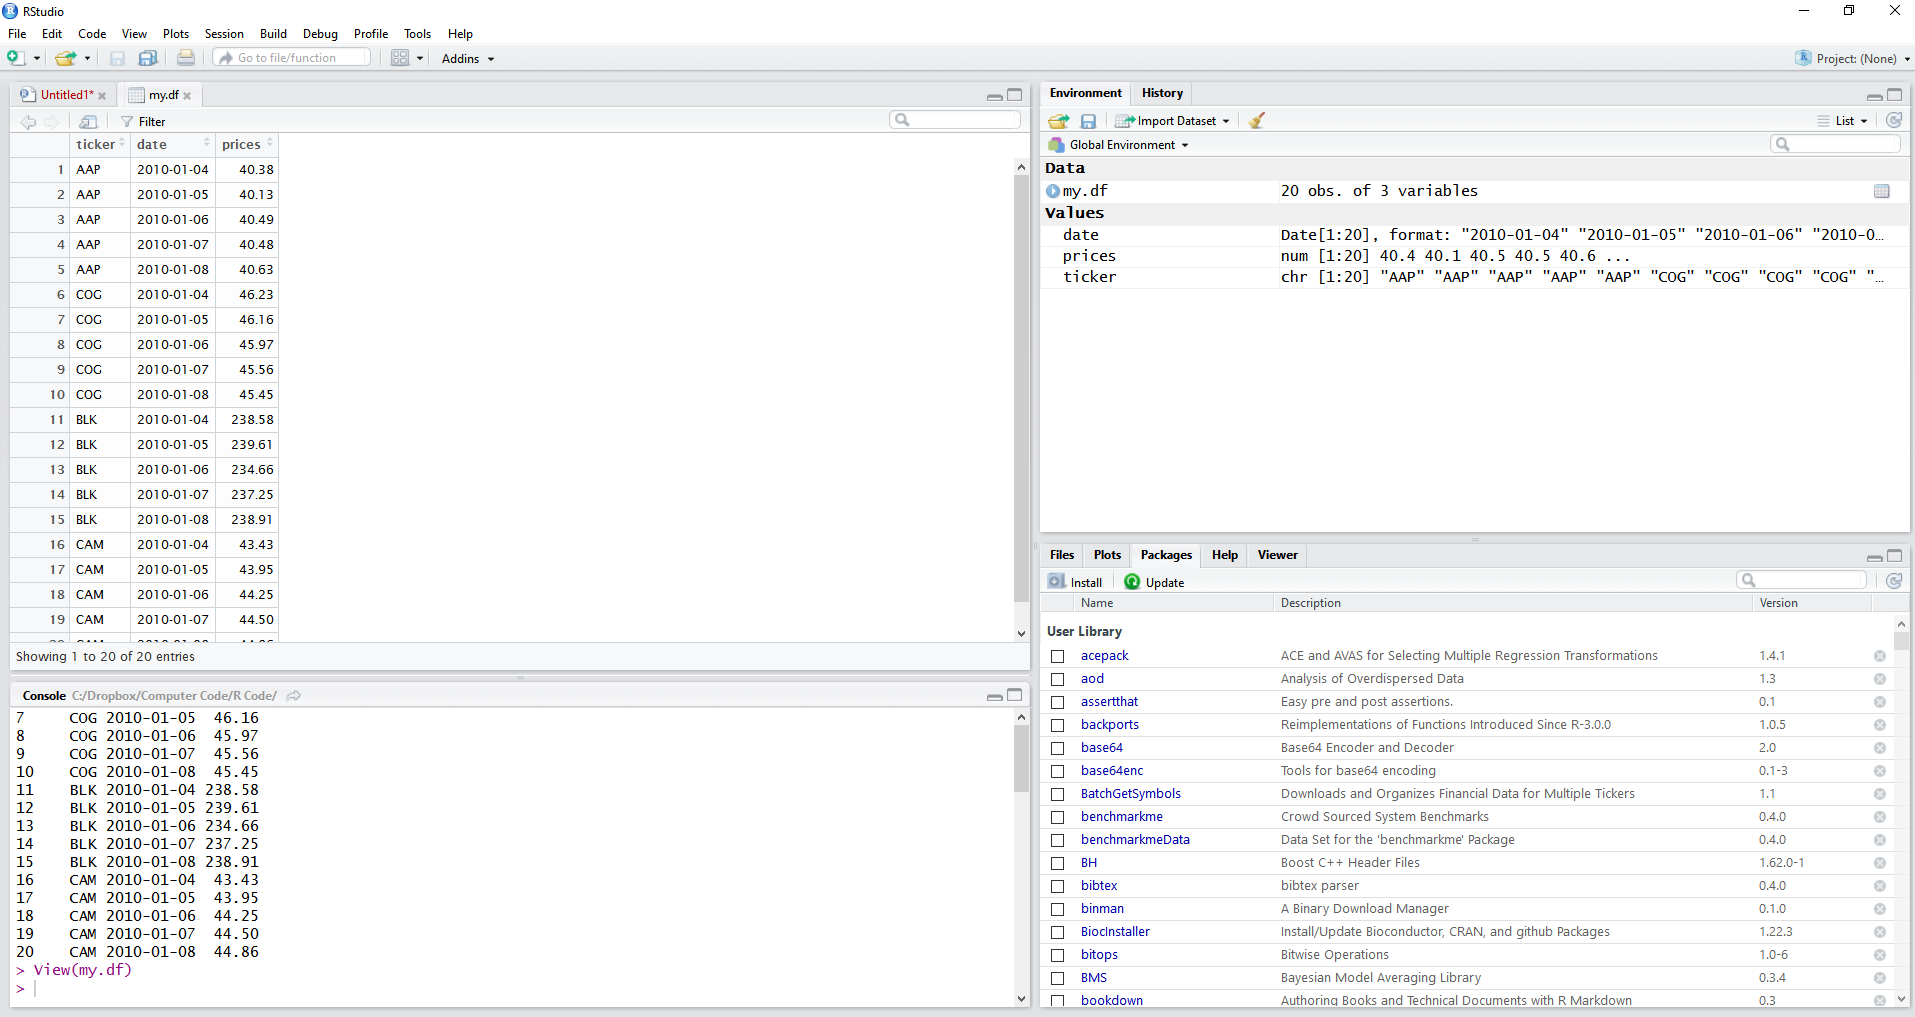
\includegraphics[width=1\linewidth]{figs/Command_view} 

}

\caption{Example of viewing a dataframe in RStudio}\label{fig:example-view}
\end{figure}

The advantages of using the viewer is that you can explore the data and
sort the columns easily, by just clicking in their names. For those who
like to use the prompt, you can open the viewer with function
\texttt{View}, as in \texttt{View(my.df)}. \index{utils!View}

\subsection{\texorpdfstring{Accessing Information from a
\texttt{dataframe}}{Accessing Information from a dataframe}}\label{accessing-information-from-a-dataframe}

A \texttt{dataframe} object makes use of same commands and symbols used
for object of type \texttt{matrix} and \texttt{list}. These functions
are generic and can be customized for different objects, including
user-created classes.

To find out the names of the columns of a \texttt{dataframe}, we have
two functions, \texttt{names} and \texttt{colnames}, with the exact same
behaviour: \index{base!names} \index{base!colnames}

\begin{Shaded}
\begin{Highlighting}[]
\CommentTok{# get names of columns with names}
\KeywordTok{names}\NormalTok{(my.df)}
\end{Highlighting}
\end{Shaded}

\begin{verbatim}
## [1] "ticker" "date"   "prices"
\end{verbatim}

\begin{Shaded}
\begin{Highlighting}[]
\CommentTok{# get names of columns with colnames}
\KeywordTok{colnames}\NormalTok{(my.df)}
\end{Highlighting}
\end{Shaded}

\begin{verbatim}
## [1] "ticker" "date"   "prices"
\end{verbatim}

To access a particular column of a \texttt{dataframe}, we can use
operator \texttt{\$} or the name/position of the column with brackets.
See next:

\begin{Shaded}
\begin{Highlighting}[]
\CommentTok{# get column ticker from my.df}
\NormalTok{my.ticker <-}\StringTok{ }\NormalTok{my.df}\OperatorTok{$}\NormalTok{ticker   }

\CommentTok{# get column price from my.df}
\NormalTok{my.prices <-}\StringTok{ }\NormalTok{my.df[}\StringTok{'prices'}\NormalTok{]}

\CommentTok{# get second column from my.df}
\NormalTok{my.date <-}\StringTok{ }\NormalTok{my.df[ ,}\DecValTok{2}\NormalTok{] }

\CommentTok{# print the results}
\KeywordTok{print}\NormalTok{(my.ticker)}
\end{Highlighting}
\end{Shaded}

\begin{verbatim}
##  [1] AAP AAP AAP AAP AAP COG COG COG COG COG BLK BLK BLK BLK
## [15] BLK CAM CAM CAM CAM CAM
## Levels: AAP BLK CAM COG
\end{verbatim}

\begin{Shaded}
\begin{Highlighting}[]
\KeywordTok{print}\NormalTok{(my.prices)}
\end{Highlighting}
\end{Shaded}

\begin{verbatim}
##    prices
## 1   40.38
## 2   40.14
## 3   40.49
## 4   40.48
## 5   40.64
## 6   46.23
## 7   46.17
## 8   45.97
## 9   45.56
## 10  45.46
## 11 238.58
## 12 239.61
## 13 234.67
## 14 237.25
## 15 238.92
## 16  43.43
## 17  43.96
## 18  44.26
## 19  44.50
## 20  44.86
\end{verbatim}

\begin{Shaded}
\begin{Highlighting}[]
\KeywordTok{print}\NormalTok{(my.date)}
\end{Highlighting}
\end{Shaded}

\begin{verbatim}
##  [1] "2010-01-04" "2010-01-05" "2010-01-06" "2010-01-07"
##  [5] "2010-01-08" "2010-01-04" "2010-01-05" "2010-01-06"
##  [9] "2010-01-07" "2010-01-08" "2010-01-04" "2010-01-05"
## [13] "2010-01-06" "2010-01-07" "2010-01-08" "2010-01-04"
## [17] "2010-01-05" "2010-01-06" "2010-01-07" "2010-01-08"
\end{verbatim}

Another important piece of information about \texttt{dataframe} objects
is, internally, they are stored as \texttt{lists}, where each element is
a column. This is important because some properties of \texttt{lists}
also work for \texttt{dataframes}. One example is using double bracket
(\texttt{{[}{[}\ {]}{]}}) for selecting columns:

\begin{Shaded}
\begin{Highlighting}[]
\CommentTok{# select column in dataframe with list notation}
\KeywordTok{print}\NormalTok{(my.df[[}\DecValTok{2}\NormalTok{]])}
\end{Highlighting}
\end{Shaded}

\begin{verbatim}
##  [1] "2010-01-04" "2010-01-05" "2010-01-06" "2010-01-07"
##  [5] "2010-01-08" "2010-01-04" "2010-01-05" "2010-01-06"
##  [9] "2010-01-07" "2010-01-08" "2010-01-04" "2010-01-05"
## [13] "2010-01-06" "2010-01-07" "2010-01-08" "2010-01-04"
## [17] "2010-01-05" "2010-01-06" "2010-01-07" "2010-01-08"
\end{verbatim}

To access specific rows and columns of a \texttt{dataframe}, use single
brackets together with atomic vectors that indicate positions:

\begin{Shaded}
\begin{Highlighting}[]
\CommentTok{# accessing rows 1:5, column 2}
\KeywordTok{print}\NormalTok{(my.df[}\DecValTok{1}\OperatorTok{:}\DecValTok{5}\NormalTok{, }\DecValTok{2}\NormalTok{])}
\end{Highlighting}
\end{Shaded}

\begin{verbatim}
## [1] "2010-01-04" "2010-01-05" "2010-01-06" "2010-01-07"
## [5] "2010-01-08"
\end{verbatim}

\begin{Shaded}
\begin{Highlighting}[]
\CommentTok{# accessing rows 1:5, columns 1 and 2}
\KeywordTok{print}\NormalTok{(my.df[}\DecValTok{1}\OperatorTok{:}\DecValTok{5}\NormalTok{, }\KeywordTok{c}\NormalTok{(}\DecValTok{1}\NormalTok{,}\DecValTok{2}\NormalTok{)])}
\end{Highlighting}
\end{Shaded}

\begin{verbatim}
##   ticker       date
## 1    AAP 2010-01-04
## 2    AAP 2010-01-05
## 3    AAP 2010-01-06
## 4    AAP 2010-01-07
## 5    AAP 2010-01-08
\end{verbatim}

\begin{Shaded}
\begin{Highlighting}[]
\CommentTok{# accessing rows 1:5, all columns}
\KeywordTok{print}\NormalTok{(my.df[}\DecValTok{1}\OperatorTok{:}\DecValTok{5}\NormalTok{, ])}
\end{Highlighting}
\end{Shaded}

\begin{verbatim}
##   ticker       date prices
## 1    AAP 2010-01-04  40.38
## 2    AAP 2010-01-05  40.14
## 3    AAP 2010-01-06  40.49
## 4    AAP 2010-01-07  40.48
## 5    AAP 2010-01-08  40.64
\end{verbatim}

Column selection can also be performed using names. Look at the
following example:

\begin{Shaded}
\begin{Highlighting}[]
\CommentTok{# selecting rows 1 to 3, columns 'ticker' and 'prices'}
\KeywordTok{print}\NormalTok{(my.df[}\DecValTok{1}\OperatorTok{:}\DecValTok{3}\NormalTok{, }\KeywordTok{c}\NormalTok{(}\StringTok{'ticker'}\NormalTok{,}\StringTok{'prices'}\NormalTok{)])}
\end{Highlighting}
\end{Shaded}

\begin{verbatim}
##   ticker prices
## 1    AAP  40.38
## 2    AAP  40.14
## 3    AAP  40.49
\end{verbatim}

\subsection{\texorpdfstring{Modifying a
\texttt{dataframe}}{Modifying a dataframe}}\label{modifying-a-dataframe}

To create a new column in a \texttt{dataframe}, simply allocate an
atomic vector of any class with the same length as the number of rows in
the existing \texttt{dataframe}. If we want to insert a sequence of
values as a new column in \texttt{my.df}, we could do it as follows:
\index{adding column to dataframe}

\begin{Shaded}
\begin{Highlighting}[]
\CommentTok{# add a sequence to my.df}
\NormalTok{my.df}\OperatorTok{$}\NormalTok{my.seq <-}\StringTok{ }\DecValTok{1}\OperatorTok{:}\KeywordTok{nrow}\NormalTok{(my.df)}

\CommentTok{# print result}
\KeywordTok{print}\NormalTok{(my.df)}
\end{Highlighting}
\end{Shaded}

\begin{verbatim}
##    ticker       date prices my.seq
## 1     AAP 2010-01-04  40.38      1
## 2     AAP 2010-01-05  40.14      2
## 3     AAP 2010-01-06  40.49      3
## 4     AAP 2010-01-07  40.48      4
## 5     AAP 2010-01-08  40.64      5
## 6     COG 2010-01-04  46.23      6
## 7     COG 2010-01-05  46.17      7
## 8     COG 2010-01-06  45.97      8
## 9     COG 2010-01-07  45.56      9
## 10    COG 2010-01-08  45.46     10
## 11    BLK 2010-01-04 238.58     11
## 12    BLK 2010-01-05 239.61     12
## 13    BLK 2010-01-06 234.67     13
## 14    BLK 2010-01-07 237.25     14
## 15    BLK 2010-01-08 238.92     15
## 16    CAM 2010-01-04  43.43     16
## 17    CAM 2010-01-05  43.96     17
## 18    CAM 2010-01-06  44.26     18
## 19    CAM 2010-01-07  44.50     19
## 20    CAM 2010-01-08  44.86     20
\end{verbatim}

You can also perform this modification of a \texttt{dataframe} with
single brackets or the position of the new column:

\begin{Shaded}
\begin{Highlighting}[]
\CommentTok{# set new col by name}
\NormalTok{my.df[}\StringTok{'my.seq.2'}\NormalTok{] <-}\StringTok{ }\KeywordTok{seq}\NormalTok{(}\DecValTok{1}\NormalTok{,}\DecValTok{100}\NormalTok{, }\DataTypeTok{length.out =} \KeywordTok{nrow}\NormalTok{(my.df))}

\CommentTok{# set new col by position}
\NormalTok{my.df[[}\DecValTok{6}\NormalTok{]] <-}\StringTok{ }\KeywordTok{seq}\NormalTok{(}\DecValTok{1}\NormalTok{,}\DecValTok{10}\NormalTok{, }\DataTypeTok{length.out =} \KeywordTok{nrow}\NormalTok{(my.df))}
\KeywordTok{print}\NormalTok{(my.df)}
\end{Highlighting}
\end{Shaded}

\begin{verbatim}
##    ticker       date prices my.seq   my.seq.2        V6
## 1     AAP 2010-01-04  40.38      1   1.000000  1.000000
## 2     AAP 2010-01-05  40.14      2   6.210526  1.473684
## 3     AAP 2010-01-06  40.49      3  11.421053  1.947368
## 4     AAP 2010-01-07  40.48      4  16.631579  2.421053
## 5     AAP 2010-01-08  40.64      5  21.842105  2.894737
## 6     COG 2010-01-04  46.23      6  27.052632  3.368421
## 7     COG 2010-01-05  46.17      7  32.263158  3.842105
## 8     COG 2010-01-06  45.97      8  37.473684  4.315789
## 9     COG 2010-01-07  45.56      9  42.684211  4.789474
## 10    COG 2010-01-08  45.46     10  47.894737  5.263158
## 11    BLK 2010-01-04 238.58     11  53.105263  5.736842
## 12    BLK 2010-01-05 239.61     12  58.315789  6.210526
## 13    BLK 2010-01-06 234.67     13  63.526316  6.684211
## 14    BLK 2010-01-07 237.25     14  68.736842  7.157895
## 15    BLK 2010-01-08 238.92     15  73.947368  7.631579
## 16    CAM 2010-01-04  43.43     16  79.157895  8.105263
## 17    CAM 2010-01-05  43.96     17  84.368421  8.578947
## 18    CAM 2010-01-06  44.26     18  89.578947  9.052632
## 19    CAM 2010-01-07  44.50     19  94.789474  9.526316
## 20    CAM 2010-01-08  44.86     20 100.000000 10.000000
\end{verbatim}

When using column position for setting a new column into a
\texttt{dataframe}, its name becomes \texttt{V6}, i.e. \emph{variable
6}. In R, when no name is entered by the user, this is the default
allocation. However, it is always good policy to name all columns of the
\texttt{dataframe} with some hint to its content. As for columns that
will not be used, simply remove them prior to processing. In our
example, we can rename the columns using function \texttt{colnames}:
\index{base!colnames}

\begin{Shaded}
\begin{Highlighting}[]
\CommentTok{# rename colnames}
\KeywordTok{colnames}\NormalTok{(my.df) <-}\StringTok{ }\KeywordTok{c}\NormalTok{(}\StringTok{'ticker'}\NormalTok{, }\StringTok{'date'}\NormalTok{, }\StringTok{'prices'}\NormalTok{, }
                     \StringTok{'my.seq'}\NormalTok{, }\StringTok{'my.seq.2'}\NormalTok{, }\StringTok{'my.seq.3'}\NormalTok{)}

\CommentTok{# print result}
\KeywordTok{print}\NormalTok{(my.df)}
\end{Highlighting}
\end{Shaded}

\begin{verbatim}
##    ticker       date prices my.seq   my.seq.2  my.seq.3
## 1     AAP 2010-01-04  40.38      1   1.000000  1.000000
## 2     AAP 2010-01-05  40.14      2   6.210526  1.473684
## 3     AAP 2010-01-06  40.49      3  11.421053  1.947368
## 4     AAP 2010-01-07  40.48      4  16.631579  2.421053
## 5     AAP 2010-01-08  40.64      5  21.842105  2.894737
## 6     COG 2010-01-04  46.23      6  27.052632  3.368421
## 7     COG 2010-01-05  46.17      7  32.263158  3.842105
## 8     COG 2010-01-06  45.97      8  37.473684  4.315789
## 9     COG 2010-01-07  45.56      9  42.684211  4.789474
## 10    COG 2010-01-08  45.46     10  47.894737  5.263158
## 11    BLK 2010-01-04 238.58     11  53.105263  5.736842
## 12    BLK 2010-01-05 239.61     12  58.315789  6.210526
## 13    BLK 2010-01-06 234.67     13  63.526316  6.684211
## 14    BLK 2010-01-07 237.25     14  68.736842  7.157895
## 15    BLK 2010-01-08 238.92     15  73.947368  7.631579
## 16    CAM 2010-01-04  43.43     16  79.157895  8.105263
## 17    CAM 2010-01-05  43.96     17  84.368421  8.578947
## 18    CAM 2010-01-06  44.26     18  89.578947  9.052632
## 19    CAM 2010-01-07  44.50     19  94.789474  9.526316
## 20    CAM 2010-01-08  44.86     20 100.000000 10.000000
\end{verbatim}

R allows using spaces in the names of columns. If we wanted a column to
be named \texttt{My\ Column\ 1}, you could set it as:

\begin{Shaded}
\begin{Highlighting}[]
\CommentTok{# set df}
\NormalTok{temp.df <-}\StringTok{ }\KeywordTok{data.frame}\NormalTok{(}\StringTok{'My Column 1'}\NormalTok{ =}\StringTok{ }\KeywordTok{runif}\NormalTok{(}\DecValTok{5}\NormalTok{), }\DataTypeTok{check.names=}\OtherTok{FALSE}\NormalTok{)}

\CommentTok{# set columns name "My Column 2" with grave accent}
\NormalTok{temp.df}\OperatorTok{$}\StringTok{`}\DataTypeTok{My column 2}\StringTok{`}\NormalTok{ <-}\StringTok{ }\KeywordTok{runif}\NormalTok{(}\DecValTok{5}\NormalTok{)}

\CommentTok{# set columns name "My Column 3" with apostrophe}
\NormalTok{temp.df}\OperatorTok{$}\StringTok{'My column 3'}\NormalTok{ <-}\StringTok{ }\KeywordTok{runif}\NormalTok{(}\DecValTok{5}\NormalTok{)}

\CommentTok{#print result}
\KeywordTok{print}\NormalTok{(temp.df)}
\end{Highlighting}
\end{Shaded}

\begin{verbatim}
##   My Column 1 My column 2 My column 3
## 1   0.3151841  0.55032776   0.1472167
## 2   0.2826696  0.64836951   0.8223904
## 3   0.7131957  0.23478670   0.4135184
## 4   0.8621379  0.07629721   0.6125206
## 5   0.1063235  0.92309504   0.0681205
\end{verbatim}

Within function \texttt{data.frame}, we need to use
\texttt{check.names=FALSE} for custom column names, otherwise the spaces
in the are converted to dots. When using \texttt{\$} or brackets, we use
the grave accent and apostrophe to encapsulate the column name. You can
access the custom column using the same notation or with brackets
(\texttt{temp.df{[}\textquotesingle{}My\ column\ 1\textquotesingle{}{]}}).
This is a great feature because it allows us to create the final version
of tables directly in R. We set the names of the columns as they should
appear in the final version of the report and export the
\texttt{dataframe} to a spreadsheet-like tool. Within this software, you
can format your table to your needs and later export it to the final
report. In later section, we will discuss a more elegant way of
exporting tables from R using specialized packages.

To remove the columns of a \texttt{dataframe}, just set the column to a
\texttt{NULL} value: \index{NULL}

\begin{Shaded}
\begin{Highlighting}[]
\CommentTok{# removing columns}
\NormalTok{my.df}\OperatorTok{$}\NormalTok{my.seq <-}\StringTok{ }\OtherTok{NULL}
\NormalTok{my.df}\OperatorTok{$}\NormalTok{my.seq.}\DecValTok{2}\NormalTok{ <-}\StringTok{ }\OtherTok{NULL}
\NormalTok{my.df}\OperatorTok{$}\NormalTok{my.seq.}\DecValTok{3}\NormalTok{ <-}\StringTok{ }\OtherTok{NULL}
\NormalTok{my.df}\OperatorTok{$}\NormalTok{V6 <-}\StringTok{ }\OtherTok{NULL}

\CommentTok{# print final result}
\KeywordTok{print}\NormalTok{(my.df[}\DecValTok{1}\OperatorTok{:}\DecValTok{5}\NormalTok{, ])}
\end{Highlighting}
\end{Shaded}

\begin{verbatim}
##   ticker       date prices
## 1    AAP 2010-01-04  40.38
## 2    AAP 2010-01-05  40.14
## 3    AAP 2010-01-06  40.49
## 4    AAP 2010-01-07  40.48
## 5    AAP 2010-01-08  40.64
\end{verbatim}

You can also remove columns using negative indices. For example, in the
following code, we create a new \texttt{dataframe} without the first and
third columns of \texttt{my.df}:

\begin{Shaded}
\begin{Highlighting}[]
\CommentTok{# create new dataframe without cols 1 and 3 of my.df}
\NormalTok{new.df <-}\StringTok{ }\NormalTok{my.df[ ,}\KeywordTok{c}\NormalTok{(}\OperatorTok{-}\DecValTok{1}\NormalTok{,}\OperatorTok{-}\DecValTok{3}\NormalTok{)]}

\CommentTok{# print result}
\KeywordTok{print}\NormalTok{(new.df)}
\end{Highlighting}
\end{Shaded}

\begin{verbatim}
##  [1] "2010-01-04" "2010-01-05" "2010-01-06" "2010-01-07"
##  [5] "2010-01-08" "2010-01-04" "2010-01-05" "2010-01-06"
##  [9] "2010-01-07" "2010-01-08" "2010-01-04" "2010-01-05"
## [13] "2010-01-06" "2010-01-07" "2010-01-08" "2010-01-04"
## [17] "2010-01-05" "2010-01-06" "2010-01-07" "2010-01-08"
\end{verbatim}

Just as we have done for matrices, indexing \texttt{dataframes} with a
logical condition is also possible. If we are only interested in stock
AAP, we can create a new \texttt{dataframe} by selecting the rows where
information for this stock is found:

\begin{Shaded}
\begin{Highlighting}[]
\CommentTok{# set logical index for selecting data about stock}
\NormalTok{my.idx <-}\StringTok{ }\NormalTok{my.df}\OperatorTok{$}\NormalTok{ticker }\OperatorTok{==}\StringTok{ 'AAP'}

\CommentTok{# create new df with index}
\NormalTok{my.df.stock <-}\StringTok{ }\NormalTok{my.df[my.idx, ]}

\CommentTok{# print result}
\KeywordTok{print}\NormalTok{(my.df.stock)}
\end{Highlighting}
\end{Shaded}

\begin{verbatim}
##   ticker       date prices
## 1    AAP 2010-01-04  40.38
## 2    AAP 2010-01-05  40.14
## 3    AAP 2010-01-06  40.49
## 4    AAP 2010-01-07  40.48
## 5    AAP 2010-01-08  40.64
\end{verbatim}

We can also interact different columns using logical objects. If we
wanted to find out the date where the stock had its highest historical
value, we can use the following code:

\begin{Shaded}
\begin{Highlighting}[]
\CommentTok{# find index with which.max}
\NormalTok{my.idx <-}\StringTok{ }\KeywordTok{which.max}\NormalTok{(my.df.stock}\OperatorTok{$}\NormalTok{price)}

\CommentTok{# get date}
\NormalTok{my.date <-}\StringTok{ }\NormalTok{my.df.stock}\OperatorTok{$}\NormalTok{date[my.idx]}

\CommentTok{# print result}
\KeywordTok{print}\NormalTok{(my.date)}
\end{Highlighting}
\end{Shaded}

\begin{verbatim}
## [1] "2010-01-08"
\end{verbatim}

Therefore, in our dataset, the highest price of stock AAP was 40.64, and
it happened in date 2010-01-08.

\subsection{\texorpdfstring{Sorting a
\texttt{dataframe}}{Sorting a dataframe}}\label{sorting-a-dataframe}

After creating or importing a \texttt{dataframe}, you can sort its rows
according to the values of any column. A common case where a sort
operation is needed is when financial data is imported, but the dates
are not ascending. Depending on the situation, it may be easier (or
expected) to deal with data where the dates are always increasing along
the rows. The sorting operation in \texttt{dataframes} is performed
using function \texttt{order}. \index{base!order}
\index{ordering dataframe}

Consider creating a \texttt{data.frame} with the following values:

\begin{Shaded}
\begin{Highlighting}[]
\CommentTok{# set new df}
\NormalTok{my.df <-}\StringTok{ }\KeywordTok{data.frame}\NormalTok{(}\DataTypeTok{col1 =} \KeywordTok{c}\NormalTok{(}\DecValTok{4}\NormalTok{,}\DecValTok{1}\NormalTok{,}\DecValTok{2}\NormalTok{), }
                    \DataTypeTok{col2 =} \KeywordTok{c}\NormalTok{(}\DecValTok{1}\NormalTok{,}\DecValTok{1}\NormalTok{,}\DecValTok{3}\NormalTok{), }
                    \DataTypeTok{col3 =} \KeywordTok{c}\NormalTok{(}\StringTok{'a'}\NormalTok{,}\StringTok{'b'}\NormalTok{,}\StringTok{'c'}\NormalTok{))}

\CommentTok{# print it                  }
\KeywordTok{print}\NormalTok{(my.df)}
\end{Highlighting}
\end{Shaded}

\begin{verbatim}
##   col1 col2 col3
## 1    4    1    a
## 2    1    1    b
## 3    2    3    c
\end{verbatim}

Function \texttt{order} returns the position of the elements for the
sorted vector. With the first column of \texttt{my.df}, the positions of
the elements in an ascending order are:

\begin{Shaded}
\begin{Highlighting}[]
\CommentTok{# set index with positions of ascending order in col1}
\NormalTok{idx <-}\StringTok{ }\KeywordTok{order}\NormalTok{(my.df}\OperatorTok{$}\NormalTok{col1)}

\CommentTok{# print it}
\KeywordTok{print}\NormalTok{(idx)}
\end{Highlighting}
\end{Shaded}

\begin{verbatim}
## [1] 2 3 1
\end{verbatim}

Therefore, when using the output of function \texttt{order} as an index
of an existing \texttt{dataframe}, you get a new version of the
\texttt{dataframe}, where all rows are set according to the ascending
values of a particular column. See next:

\begin{Shaded}
\begin{Highlighting}[]
\CommentTok{# order my.df by col1}
\NormalTok{my.df.}\DecValTok{2}\NormalTok{ <-}\StringTok{ }\NormalTok{my.df[}\KeywordTok{order}\NormalTok{(my.df}\OperatorTok{$}\NormalTok{col1), ]}

\CommentTok{# print result}
\KeywordTok{print}\NormalTok{(my.df.}\DecValTok{2}\NormalTok{)}
\end{Highlighting}
\end{Shaded}

\begin{verbatim}
##   col1 col2 col3
## 2    1    1    b
## 3    2    3    c
## 1    4    1    a
\end{verbatim}

This operation may also be performed considering more than one column.
See the following example, where we sort the rows of \texttt{my.df}
using columns \texttt{col2} and \texttt{col1}.

\begin{Shaded}
\begin{Highlighting}[]
\CommentTok{# sort df with col2 and col1}
\NormalTok{my.df.}\DecValTok{3}\NormalTok{ <-}\StringTok{ }\NormalTok{my.df[}\KeywordTok{order}\NormalTok{(my.df}\OperatorTok{$}\NormalTok{col2, my.df}\OperatorTok{$}\NormalTok{col1), ]}

\CommentTok{# print result}
\KeywordTok{print}\NormalTok{(my.df.}\DecValTok{3}\NormalTok{)}
\end{Highlighting}
\end{Shaded}

\begin{verbatim}
##   col1 col2 col3
## 2    1    1    b
## 1    4    1    a
## 3    2    3    c
\end{verbatim}

\subsection{\texorpdfstring{Combining and Aggregating
\texttt{dataframes}}{Combining and Aggregating dataframes}}\label{combining-and-aggregating-dataframes}

Sometimes, it is necessary to join different \texttt{dataframes}. This
usually happens when the data is imported from different sources, and we
need to combine them into a single object in R. In the simplest case of
combining data frames, we join them according to the rows (vertically)
or columns (horizontally). For that, we have functions \texttt{rbind}
(row bind) and \texttt{cbind} (column bind). Examples of usage are given
next. \index{base!rbind} \index{base!cbind}

\begin{Shaded}
\begin{Highlighting}[]
\CommentTok{# set two dfs with same colnames}
\NormalTok{my.df.}\DecValTok{1}\NormalTok{ <-}\StringTok{ }\KeywordTok{data.frame}\NormalTok{(}\DataTypeTok{col1 =} \DecValTok{1}\OperatorTok{:}\DecValTok{5}\NormalTok{, }\DataTypeTok{col2 =} \KeywordTok{rep}\NormalTok{(}\StringTok{'a'}\NormalTok{, }\DecValTok{5}\NormalTok{))}
\NormalTok{my.df.}\DecValTok{2}\NormalTok{ <-}\StringTok{ }\KeywordTok{data.frame}\NormalTok{(}\DataTypeTok{col1 =} \DecValTok{6}\OperatorTok{:}\DecValTok{10}\NormalTok{, }\DataTypeTok{col2 =} \KeywordTok{rep}\NormalTok{(}\StringTok{'b'}\NormalTok{, }\DecValTok{5}\NormalTok{))}

\CommentTok{# bind them by rows}
\NormalTok{my.df <-}\StringTok{ }\KeywordTok{rbind}\NormalTok{(my.df.}\DecValTok{1}\NormalTok{, my.df.}\DecValTok{2}\NormalTok{)}

\CommentTok{# print result}
\KeywordTok{print}\NormalTok{(my.df)}
\end{Highlighting}
\end{Shaded}

\begin{verbatim}
##    col1 col2
## 1     1    a
## 2     2    a
## 3     3    a
## 4     4    a
## 5     5    a
## 6     6    b
## 7     7    b
## 8     8    b
## 9     9    b
## 10   10    b
\end{verbatim}

Notice, in the previous example, the names of the columns are the same.
Function \texttt{rbind} searches for equal names in both
\texttt{dataframes}. This means, if we swapped the positions of the
columns, there would be no change in the result of the bind operation.
If the names of the columns don't match, an error is returned. See next:

\begin{Shaded}
\begin{Highlighting}[]
\CommentTok{# set two df with different colnames}
\NormalTok{my.df.}\DecValTok{1}\NormalTok{ <-}\StringTok{ }\KeywordTok{data.frame}\NormalTok{(}\DataTypeTok{col1 =} \DecValTok{1}\OperatorTok{:}\DecValTok{5}\NormalTok{, }
                      \DataTypeTok{col2 =} \KeywordTok{rep}\NormalTok{(}\StringTok{'a'}\NormalTok{, }\DecValTok{5}\NormalTok{))}
\NormalTok{my.df.}\DecValTok{2}\NormalTok{ <-}\StringTok{ }\KeywordTok{data.frame}\NormalTok{(}\DataTypeTok{col1 =} \DecValTok{6}\OperatorTok{:}\DecValTok{10}\NormalTok{, }
                      \DataTypeTok{col3 =} \KeywordTok{rep}\NormalTok{(}\StringTok{'b'}\NormalTok{, }\DecValTok{5}\NormalTok{))}

\CommentTok{# bind them by rows (ERROR)}
\NormalTok{my.df <-}\StringTok{ }\KeywordTok{rbind}\NormalTok{(my.df.}\DecValTok{1}\NormalTok{, my.df.}\DecValTok{2}\NormalTok{)}
\end{Highlighting}
\end{Shaded}

\begin{verbatim}
## ##Error in match.names(clabs, names(xi)) :
##  names do not match previous names
\end{verbatim}

In the case where you have various \texttt{dataframes} with different
column names and a row bind operation is necessary, one solution is to
use function \texttt{bind\_rows} of package \texttt{dplyr}, which places
\texttt{NA} values whenever a missing column is found. Have a look:
\index{dplyr!bind\_rows}

\begin{Shaded}
\begin{Highlighting}[]
\CommentTok{# load package}
\KeywordTok{library}\NormalTok{(dplyr)}

\CommentTok{# bind them by rows}
\NormalTok{my.df <-}\StringTok{ }\KeywordTok{bind_rows}\NormalTok{(my.df.}\DecValTok{1}\NormalTok{, }
\NormalTok{                   my.df.}\DecValTok{2}\NormalTok{)}

\CommentTok{# print result (NAs where there should be a column)}
\KeywordTok{print}\NormalTok{(my.df)}
\end{Highlighting}
\end{Shaded}

\begin{verbatim}
##    col1 col2
## 1     1    a
## 2     2    a
## 3     3    a
## 4     4    a
## 5     5    a
## 6     6    b
## 7     7    b
## 8     8    b
## 9     9    b
## 10   10    b
\end{verbatim}

For the case of column bind with function \texttt{cbind}, the names of
the columns must be different, but the number of rows must be the same.
See an example next. \index{base!cbind}

\begin{Shaded}
\begin{Highlighting}[]
\CommentTok{# set two dfs}
\NormalTok{my.df.}\DecValTok{1}\NormalTok{ <-}\StringTok{ }\KeywordTok{data.frame}\NormalTok{(}\DataTypeTok{col1 =} \DecValTok{1}\OperatorTok{:}\DecValTok{5}\NormalTok{, }\DataTypeTok{col2 =} \KeywordTok{rep}\NormalTok{(}\StringTok{'a'}\NormalTok{, }\DecValTok{5}\NormalTok{))}
\NormalTok{my.df.}\DecValTok{2}\NormalTok{ <-}\StringTok{ }\KeywordTok{data.frame}\NormalTok{(}\DataTypeTok{col3 =} \DecValTok{6}\OperatorTok{:}\DecValTok{10}\NormalTok{, }\DataTypeTok{col4 =} \KeywordTok{rep}\NormalTok{(}\StringTok{'b'}\NormalTok{, }\DecValTok{5}\NormalTok{))}

\CommentTok{# column bind dfs}
\NormalTok{my.df <-}\StringTok{ }\KeywordTok{cbind}\NormalTok{(my.df.}\DecValTok{1}\NormalTok{, my.df.}\DecValTok{2}\NormalTok{)}

\CommentTok{# print result}
\KeywordTok{print}\NormalTok{(my.df)}
\end{Highlighting}
\end{Shaded}

\begin{verbatim}
##   col1 col2 col3 col4
## 1    1    a    6    b
## 2    2    a    7    b
## 3    3    a    8    b
## 4    4    a    9    b
## 5    5    a   10    b
\end{verbatim}

If the number of rows don't match, an error is returned by
\texttt{cbind}. But, if the names of columns are the same, the function
still accepts the inputs. Have a look:

\begin{Shaded}
\begin{Highlighting}[]
\CommentTok{# set two dfs with same name in one}
\NormalTok{my.df.}\DecValTok{1}\NormalTok{ <-}\StringTok{ }\KeywordTok{data.frame}\NormalTok{(}\DataTypeTok{col1 =} \DecValTok{1}\OperatorTok{:}\DecValTok{5}\NormalTok{, }\DataTypeTok{col2 =} \KeywordTok{rep}\NormalTok{(}\StringTok{'a'}\NormalTok{, }\DecValTok{5}\NormalTok{))}
\NormalTok{my.df.}\DecValTok{2}\NormalTok{ <-}\StringTok{ }\KeywordTok{data.frame}\NormalTok{(}\DataTypeTok{col1 =} \DecValTok{6}\OperatorTok{:}\DecValTok{10}\NormalTok{)}

\CommentTok{# column bind dfs}
\NormalTok{my.df <-}\StringTok{ }\KeywordTok{cbind}\NormalTok{(my.df.}\DecValTok{1}\NormalTok{, my.df.}\DecValTok{2}\NormalTok{)}

\CommentTok{# print result (!)}
\KeywordTok{print}\NormalTok{(my.df)}
\end{Highlighting}
\end{Shaded}

\begin{verbatim}
##   col1 col2 col1
## 1    1    a    6
## 2    2    a    7
## 3    3    a    8
## 4    4    a    9
## 5    5    a   10
\end{verbatim}

Yes, we have two columns named \texttt{col1}, but in different
positions. If we accessed \texttt{my.df\$col1}, it returns the first
column. This is a strange behaviour of R. You should pay attention to
these cases to avoid bugs in the code.

For more complex cases, where the binding process must happen according
to some index, such as dates, it is possible to combine two
\texttt{dataframes} using function \texttt{merge}: \index{base!merge}

\begin{Shaded}
\begin{Highlighting}[]
\CommentTok{# set dfs}
\NormalTok{my.df.}\DecValTok{1}\NormalTok{ <-}\StringTok{ }\KeywordTok{data.frame}\NormalTok{(}\DataTypeTok{date =} \KeywordTok{as.Date}\NormalTok{(}\StringTok{'2016-01-01'}\NormalTok{)}\OperatorTok{+}\DecValTok{0}\OperatorTok{:}\DecValTok{10}\NormalTok{, }
                      \DataTypeTok{x =} \DecValTok{1}\OperatorTok{:}\DecValTok{11}\NormalTok{)}

\NormalTok{my.df.}\DecValTok{2}\NormalTok{ <-}\StringTok{ }\KeywordTok{data.frame}\NormalTok{(}\DataTypeTok{date =} \KeywordTok{as.Date}\NormalTok{(}\StringTok{'2016-01-05'}\NormalTok{)}\OperatorTok{+}\DecValTok{0}\OperatorTok{:}\DecValTok{10}\NormalTok{,}
                      \DataTypeTok{y =} \KeywordTok{seq}\NormalTok{(}\DecValTok{20}\NormalTok{,}\DecValTok{30}\NormalTok{, }\DataTypeTok{length.out =} \DecValTok{11}\NormalTok{))}

\CommentTok{# merge dfs by date                   }
\NormalTok{my.df <-}\StringTok{ }\KeywordTok{merge}\NormalTok{(my.df.}\DecValTok{1}\NormalTok{, my.df.}\DecValTok{2}\NormalTok{, }\DataTypeTok{by =} \StringTok{'date'}\NormalTok{)}

\CommentTok{# print result}
\KeywordTok{print}\NormalTok{(my.df)}
\end{Highlighting}
\end{Shaded}

\begin{verbatim}
##         date  x  y
## 1 2016-01-05  5 20
## 2 2016-01-06  6 21
## 3 2016-01-07  7 22
## 4 2016-01-08  8 23
## 5 2016-01-09  9 24
## 6 2016-01-10 10 25
## 7 2016-01-11 11 26
\end{verbatim}

From the result, we can see the resulting \texttt{dataframe} retained
only the information shared between the two objects, the rows where
columns \texttt{date} are equal in both \texttt{dataframes}.

Another usefull function is \texttt{match}, which does a look up
operation in vectors. For example, if we wanted to find the indices in
\texttt{my.df.2} that match the dates in \texttt{my.df.1}, we can write:

\begin{Shaded}
\begin{Highlighting}[]
\CommentTok{# set lookup index}
\NormalTok{idx <-}\StringTok{ }\KeywordTok{match}\NormalTok{(my.df.}\DecValTok{1}\OperatorTok{$}\NormalTok{date, my.df.}\DecValTok{2}\OperatorTok{$}\NormalTok{date)}

\CommentTok{# print result}
\KeywordTok{print}\NormalTok{(idx)}
\end{Highlighting}
\end{Shaded}

\begin{verbatim}
##  [1] NA NA NA NA  1  2  3  4  5  6  7
\end{verbatim}

Now we can use the index to set a new column in \texttt{my.df.1} with
data from \texttt{my.df.2}:

\begin{Shaded}
\begin{Highlighting}[]
\CommentTok{# use idx to set col in my.df.1}
\NormalTok{my.df.}\DecValTok{1}\OperatorTok{$}\NormalTok{y.}\DecValTok{2}\NormalTok{ <-}\StringTok{ }\NormalTok{my.df.}\DecValTok{2}\OperatorTok{$}\NormalTok{y[idx]}

\CommentTok{# print result}
\KeywordTok{print}\NormalTok{(my.df.}\DecValTok{1}\NormalTok{)}
\end{Highlighting}
\end{Shaded}

\begin{verbatim}
##          date  x y.2
## 1  2016-01-01  1  NA
## 2  2016-01-02  2  NA
## 3  2016-01-03  3  NA
## 4  2016-01-04  4  NA
## 5  2016-01-05  5  20
## 6  2016-01-06  6  21
## 7  2016-01-07  7  22
## 8  2016-01-08  8  23
## 9  2016-01-09  9  24
## 10 2016-01-10 10  25
## 11 2016-01-11 11  26
\end{verbatim}

A different from the use of \texttt{merge} is that \texttt{NA} values
are set where there is not matching date.

\subsection{\texorpdfstring{Reporting a \texttt{Dataframe}
Table}{Reporting a Dataframe Table}}\label{reporting-a-dataframe-table}

\texttt{Dataframes} can be used to represent and export tables to text
editing softwares, such as Word and LaTeX. The simplest way of exporting
a table from a \texttt{dataframe} object is to write it in a
spreadsheet-like tool, format it, and export the final version to the
report. Specific packages can write a \texttt{dataframe} table in an
Excel file. We will study these packages in chapter \ref{importing}.

A more elaborate way is to remove the middle man and export the table
directly from R to a LaTeX or Word file. Let's start with an example for
LaTeX. In the next chunk of code, we will create a print-ready table as
a \texttt{dataframe} and export it to a LaTeX file using package
\texttt{xtable}. \index{xtable} \index{xtable!xtable}

\begin{Shaded}
\begin{Highlighting}[]
\CommentTok{# set number of rows in table}
\NormalTok{N =}\StringTok{ }\DecValTok{10}

\CommentTok{# create artifitial data}
\KeywordTok{set.seed}\NormalTok{(}\DecValTok{20}\NormalTok{)}
\NormalTok{my.returns <-}\StringTok{ }\KeywordTok{matrix}\NormalTok{(}\KeywordTok{rnorm}\NormalTok{(}\DecValTok{50}\OperatorTok{*}\NormalTok{N), }\DataTypeTok{ncol =}\NormalTok{ N)}

\CommentTok{# set columns of df}
\NormalTok{my.names <-}\StringTok{ }\KeywordTok{paste}\NormalTok{(}\StringTok{'Stock'}\NormalTok{,}\DecValTok{1}\OperatorTok{:}\NormalTok{N)}
\NormalTok{my.mean.return <-}\StringTok{ }\KeywordTok{colMeans}\NormalTok{(my.returns)}
\NormalTok{my.sd.return <-}\StringTok{ }\KeywordTok{apply}\NormalTok{(my.returns, sd, }\DataTypeTok{MARGIN =} \DecValTok{2}\NormalTok{)}
\NormalTok{my.max.return <-}\StringTok{ }\KeywordTok{apply}\NormalTok{(my.returns, max, }\DataTypeTok{MARGIN =} \DecValTok{2}\NormalTok{)}
\NormalTok{my.min.return <-}\StringTok{ }\KeywordTok{apply}\NormalTok{(my.returns, min, }\DataTypeTok{MARGIN =} \DecValTok{2}\NormalTok{)}

\CommentTok{# set table}
\NormalTok{my.table <-}\StringTok{ }\KeywordTok{data.frame}\NormalTok{(}\StringTok{'Stocks'}\NormalTok{ =}\StringTok{ }\NormalTok{my.names,}
                       \StringTok{'Mean Ret.'}\NormalTok{ =}\StringTok{ }\NormalTok{my.mean.return,}
                       \StringTok{'StDev. of Ret.'}\NormalTok{ =}\StringTok{ }\NormalTok{my.sd.return,}
                       \StringTok{'Max. Ret.'}\NormalTok{ =}\StringTok{ }\NormalTok{my.max.return,}
                       \StringTok{'Min. Ret.'}\NormalTok{ =}\StringTok{ }\NormalTok{my.min.return, }
                       \DataTypeTok{check.names =}\NormalTok{ F)}
\end{Highlighting}
\end{Shaded}

The artificial data was set as a \texttt{matrix} object containing
random values from the Normal distribution. Each stock has its returns
as a column in \texttt{my.returns}. Several statistics for each column
are calculated using function \texttt{apply}. This function allows the
user to apply a procedure to several columns of a \texttt{matrix}. We
will study it further in chapter \ref{programming}.

In the creation of the \texttt{dataframe}, notice how we used column
names with space by encapsulating the text with apostrophes. It was also
necessary to use input \texttt{check.names\ =\ FALSE}, so R does not
change the original name of the columns. Now that we have our data,
let's export it to LaTeX.

\begin{Shaded}
\begin{Highlighting}[]
\KeywordTok{library}\NormalTok{(xtable)}

\CommentTok{# set xtable object}
\NormalTok{my.xtable <-}\StringTok{ }\KeywordTok{xtable}\NormalTok{(}\DataTypeTok{x =}\NormalTok{ my.table, }
                    \DataTypeTok{label =} \StringTok{'tab:DescRetStats'}\NormalTok{,}
                    \DataTypeTok{caption =} \StringTok{'Descriptive Statistics for Returns'}\NormalTok{)}

\CommentTok{# check if folder exists}
\ControlFlowTok{if}\NormalTok{ (}\OperatorTok{!}\KeywordTok{dir.exists}\NormalTok{(}\StringTok{'tabs'}\NormalTok{)) \{ }
    \KeywordTok{dir.create}\NormalTok{(}\StringTok{'tabs'}\NormalTok{)}
\NormalTok{\}}

\CommentTok{# print output to latex file}
\NormalTok{my.f.tex <-}\StringTok{ 'tabs/MyTable.tex'}

\CommentTok{# save it}
\KeywordTok{print}\NormalTok{(my.xtable,}
      \DataTypeTok{include.rownames =} \OtherTok{FALSE}\NormalTok{,}
      \DataTypeTok{file =}\NormalTok{ my.f.tex,}
      \DataTypeTok{type=}\StringTok{'latex'}\NormalTok{)}
\end{Highlighting}
\end{Shaded}

In function \texttt{xtable}, we kept it simple by only using arguments
\texttt{caption} and \texttt{label}. The resulting LaTeX file is saved
in folder \texttt{tabs} of the current directory. If it doesn't exist,
you can create it with
\texttt{dir.create(\textquotesingle{}tabs\textquotesingle{})}. There are
many more options for customization. The result in a compiled latex file
will be identical to \ref{fig:table-xtable}, a print-ready material for
an scientific article or report.

\begin{figure}[!htbp]

{\centering 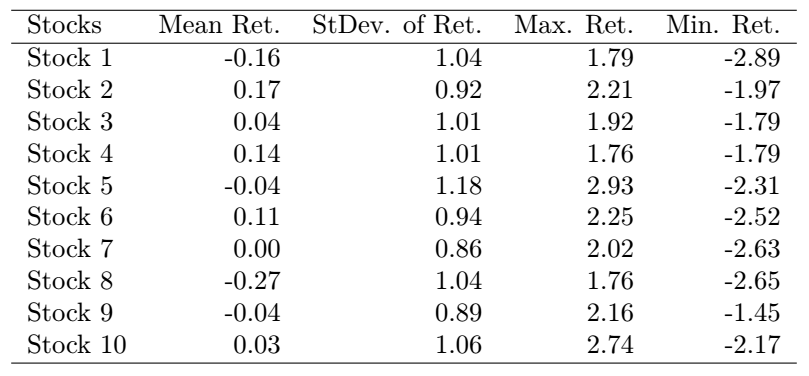
\includegraphics[width=0.75\linewidth]{tabs/table-4-2} 

}

\caption{Example of table with xtable}\label{fig:table-xtable}
\end{figure}

Another interesting package worth mentioning at this stage is
\texttt{stargazer}. Like \texttt{texreg}, it provides many options for
customizing a table and exporting it. One innovation over
\texttt{texreg} is it offers templates for journals, such as a table
template for \emph{American Economic Review}, \emph{Quarterly Journal of
Economics}, and others. Let's give it a try by replicating the previous
table. In the next code, we again use object \texttt{my.table} to export
a LaTeX table. The result is reported in \ref{fig:table-stargazer}.
\index{stargazer} \index{stargazer!stargazer}

\begin{Shaded}
\begin{Highlighting}[]
\KeywordTok{library}\NormalTok{(stargazer)}

\NormalTok{my.stargazer <-}\StringTok{ }\KeywordTok{stargazer}\NormalTok{(my.table, }
                          \DataTypeTok{summary =} \OtherTok{FALSE}\NormalTok{, }
                          \DataTypeTok{title =} \StringTok{'Descriptive Statistics for Returns'}\NormalTok{, }
                          \DataTypeTok{type =} \StringTok{'latex'}\NormalTok{, }
                          \DataTypeTok{style =} \StringTok{'qje'}\NormalTok{, }
                          \DataTypeTok{font.size =} \StringTok{'footnotesize'}\NormalTok{, }
                          \DataTypeTok{rownames =} \OtherTok{FALSE}\NormalTok{, }
                          \DataTypeTok{out.header =} \OtherTok{FALSE}\NormalTok{,}
                          \DataTypeTok{header =} \OtherTok{FALSE}\NormalTok{,}
                          \DataTypeTok{label =} \StringTok{'tab:DescRetStats_stargazer'}\NormalTok{ )}
\end{Highlighting}
\end{Shaded}

\begin{figure}[!htbp]

{\centering 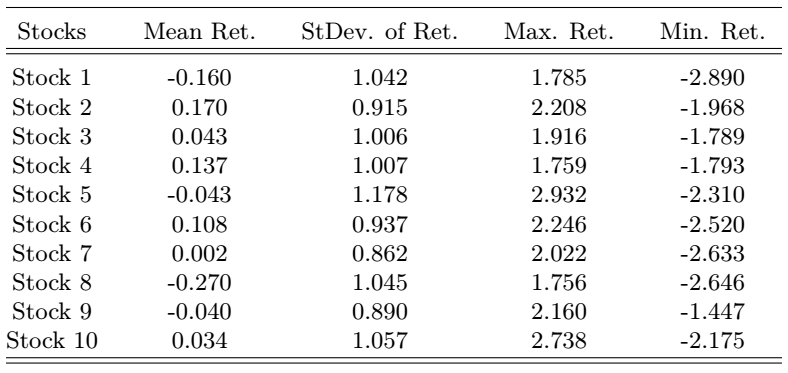
\includegraphics[width=0.75\linewidth]{tabs/table-4-3} 

}

\caption{Example of table with stargazer}\label{fig:table-stargazer}
\end{figure}

As for exporting tables to Word (Microsoft) or Writer (Libreoffice)
files, there is no direct way of doing so using \texttt{xtable} or
\texttt{stargazer}. But, a simple workaround is to use either package to
output a table to a temporary \emph{.html} or \emph{.doc} file and then
copy and paste the result in the final report. This operation works
because \emph{.html} and \emph{.doc} files share a similar format for
tables. Let's try it. First, we will save the table in a new file with
the \emph{.html} extension:

\begin{Shaded}
\begin{Highlighting}[]
\CommentTok{# set html file for output}
\NormalTok{my.f.html <-}\StringTok{ 'tabs/MyTable.html'}

\CommentTok{# write it!}
\KeywordTok{print}\NormalTok{(}\DataTypeTok{x =}\NormalTok{ my.xtable,}
      \DataTypeTok{file =}\NormalTok{ my.f.html,}
      \DataTypeTok{type =} \StringTok{'html'}\NormalTok{,}
      \DataTypeTok{include.rownames =} \OtherTok{FALSE}\NormalTok{ )}
\end{Highlighting}
\end{Shaded}

Once the file is available, we can open tabs/MyTable.html with any web
browser, select and copy the table and, finally, paste it in our
\emph{.docx} document. The result should look like Figure
\ref{fig:Writer-TableExample}.

\begin{figure}[!htbp]

{\centering 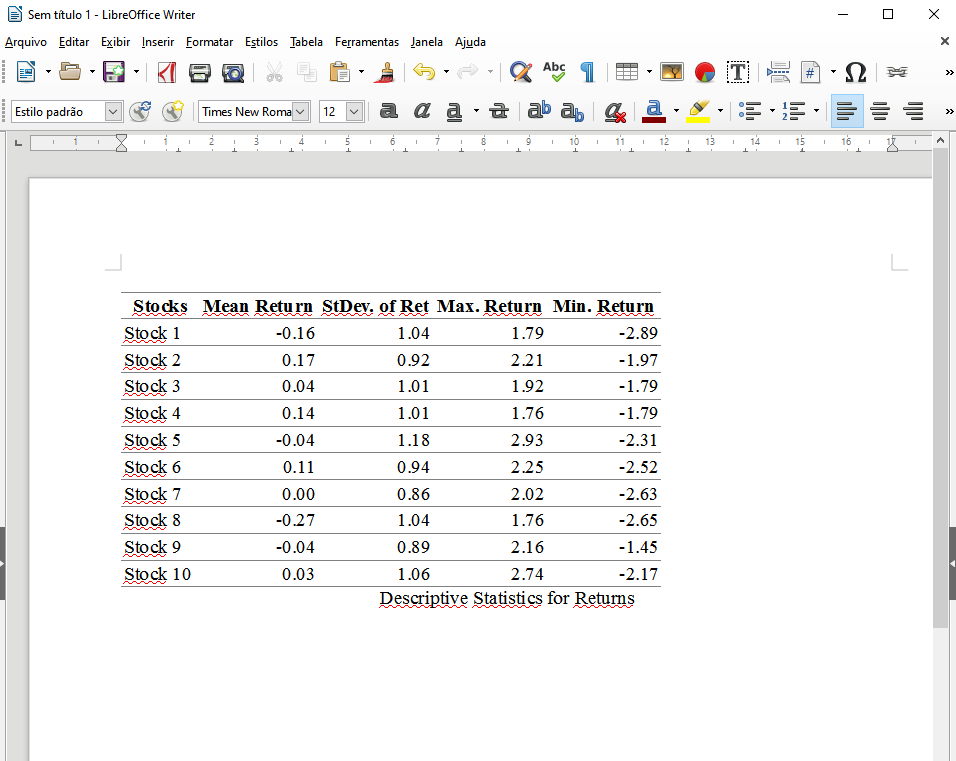
\includegraphics[width=0.75\linewidth]{figs/Writer-TableExample} 

}

\caption{Example of table in Writer (LibreOffice)}\label{fig:Writer-TableExample}
\end{figure}

If you deal with lots of figures and tables in \emph{.docx}
(Word/Writer) or \emph{.ppt} (Powerpoint/Impress) files, packages
\texttt{knitr} \citep{knitr} and \texttt{ReporteRs} \citep{reporters}
can save you a lot of time and effort. Both have extensive capabilities
of automating the process of creating reports. \index{knitr}
\index{reportr}

\subsection{\texorpdfstring{The Format of the \texttt{dataframe}
(\emph{long} and
\emph{wide})}{The Format of the dataframe (long and wide)}}\label{the-format-of-the-dataframe-long-and-wide}

After understanding the basics of \texttt{dataframe} manipulation, it is
important to discuss the format of the object and how it facilitates
future work. This is a relatively new topic that came up with the
introduction of specific packages for data manipulation and graphics. At
the heart of the debate, we discuss whether the data should be guided by
columns (\emph{wide} format) or lines (\emph{long} format).
\index{long format} \index{wide format}

\textbf{In the wide format}, the rows are usually indexed by a single
factor, such as a date, and the columns indicate the different
variables. As new information is added to the database, it usually grows
in the number of columns. An example:

\begin{tabular}{l|r|r|r}
\hline
refdate & STOCK1 & STOCK2 & STOCK3\\
\hline
2017-05-04 & 10.02 & 3.15 & 5.19\\
\hline
2017-05-05 & 9.79 & 3.34 & 5.06\\
\hline
2017-05-06 & 8.08 & 2.74 & 5.61\\
\hline
2017-05-07 & 7.33 & 2.56 & 5.99\\
\hline
\end{tabular}

Note, the above table has three distinct pieces of information for each
data point: ticker, price, and date. If we added one more stock, the
table would be incremented by one column. If we wanted to include a new
variable such as traded volume, we would need to create a new table or a
structured naming system for the columns.

\textbf{In the long format}, each row of the \texttt{dataframe} is new
information and each column is a variable. Table rows may or may not be
unique (does not repeat). As new data is added, the table usually grows
in the number of rows. Example:

\begin{tabular}{l|l|r}
\hline
refdate & ticker & price\\
\hline
2017-05-04 & STOCK1 & 10.02\\
\hline
2017-05-05 & STOCK1 & 9.79\\
\hline
2017-05-06 & STOCK1 & 8.08\\
\hline
2017-05-07 & STOCK1 & 7.33\\
\hline
2017-05-04 & STOCK2 & 3.15\\
\hline
2017-05-05 & STOCK2 & 3.34\\
\hline
2017-05-06 & STOCK2 & 2.74\\
\hline
2017-05-07 & STOCK2 & 2.56\\
\hline
2017-05-04 & STOCK3 & 5.19\\
\hline
2017-05-05 & STOCK3 & 5.06\\
\hline
2017-05-06 & STOCK3 & 5.61\\
\hline
2017-05-07 & STOCK3 & 5.99\\
\hline
\end{tabular}

This argument may seem trivial since the information is the same in both
formats. But, make no mistake: the format of the data is very important
and may facilitate the analysis of the data. Specialized packages, such
as \texttt{dplyr} \citep{dplyr} and \texttt{ggplot2}
\citep{wickham2009ggplot2}, expect a \texttt{dataframe} in the
\emph{long} format; therefore, this structure must be prioritized if one
is using these packages.

In finance, the wide format is used in the creation and manipulation of
investment portfolios with the creation of a matrix of returns. This
matrix separates the different assets by columns and rows representing
different time periods. Each value in the matrix is the return (percent
change) of a particular asset from one period to the other. The wide
format is justified as the matrix notation facilitates matrix
calculations. I emphasize, however, these same calculations could also
be performed with the \emph{long} format. Conversion between formats is
also possible, as we will see next.

\subsubsection{\texorpdfstring{Converting a \texttt{dataframe} Structure
(long and
wide)}{Converting a dataframe Structure (long and wide)}}\label{converting-a-dataframe-structure-long-and-wide}

The conversion from one format to the other is possible with the
\texttt{tidyr} package \citep{tidyr}. See the following example, where
we change the \emph{wide} format of the previous table for the
\emph{long} format using function \texttt{gather}. Here, it is necessary
to know the variable \texttt{id} that will index the lines (in this
case, the dates) and the names of the new columns. \index{tidyr}
\index{tidyr!gather}

\begin{Shaded}
\begin{Highlighting}[]
\KeywordTok{library}\NormalTok{(tidyr)}

\CommentTok{# set dates and stock vectors}
\NormalTok{refdate <-}\StringTok{ }\KeywordTok{as.Date}\NormalTok{(}\StringTok{'2015-01-01'}\NormalTok{) }\OperatorTok{+}\StringTok{ }\DecValTok{0}\OperatorTok{:}\DecValTok{3}
\NormalTok{STOCK1 <-}\StringTok{ }\KeywordTok{c}\NormalTok{(}\DecValTok{10}\NormalTok{, }\DecValTok{11}\NormalTok{, }\FloatTok{10.5}\NormalTok{, }\DecValTok{12}\NormalTok{)}
\NormalTok{STOCK2 <-}\StringTok{ }\KeywordTok{c}\NormalTok{(}\DecValTok{3}\NormalTok{, }\FloatTok{3.1}\NormalTok{, }\FloatTok{3.2}\NormalTok{, }\FloatTok{3.5}\NormalTok{)}
\NormalTok{STOCK3 <-}\StringTok{ }\KeywordTok{c}\NormalTok{(}\DecValTok{6}\NormalTok{, }\DecValTok{7}\NormalTok{, }\FloatTok{7.5}\NormalTok{, }\DecValTok{6}\NormalTok{)}

\CommentTok{# create wide dataframe}
\NormalTok{my.df.wide <-}\StringTok{ }\KeywordTok{data.frame}\NormalTok{(refdate, STOCK1, STOCK2, STOCK3)}

\CommentTok{# convert wide to long}
\NormalTok{my.df.long <-}\StringTok{ }\KeywordTok{gather}\NormalTok{(}\DataTypeTok{data =}\NormalTok{ my.df.wide,}
                     \DataTypeTok{key =} \StringTok{'ticker'}\NormalTok{,}
                     \DataTypeTok{value =} \StringTok{'price'}\NormalTok{,}
                     \OperatorTok{-}\StringTok{ }\NormalTok{refdate)}

\CommentTok{# print result}
\KeywordTok{print}\NormalTok{(my.df.long)}
\end{Highlighting}
\end{Shaded}

\begin{verbatim}
##       refdate ticker price
## 1  2015-01-01 STOCK1  10.0
## 2  2015-01-02 STOCK1  11.0
## 3  2015-01-03 STOCK1  10.5
## 4  2015-01-04 STOCK1  12.0
## 5  2015-01-01 STOCK2   3.0
## 6  2015-01-02 STOCK2   3.1
## 7  2015-01-03 STOCK2   3.2
## 8  2015-01-04 STOCK2   3.5
## 9  2015-01-01 STOCK3   6.0
## 10 2015-01-02 STOCK3   7.0
## 11 2015-01-03 STOCK3   7.5
## 12 2015-01-04 STOCK3   6.0
\end{verbatim}

To perform the reverse conversion, \emph{long} to \emph{wide}, we can
use the \texttt{spread} function from the same package, \texttt{tidyr}:
\index{tidyr!spread}

\begin{Shaded}
\begin{Highlighting}[]
\CommentTok{# convert from long to wide}
\NormalTok{my.df.wide.converted <-}\StringTok{ }\KeywordTok{spread}\NormalTok{(}\DataTypeTok{data =}\NormalTok{ my.df.long, }
                               \DataTypeTok{key =} \StringTok{'ticker'}\NormalTok{,}
                               \DataTypeTok{value =} \StringTok{'price'}\NormalTok{)}

\CommentTok{# print result}
\KeywordTok{print}\NormalTok{(my.df.wide.converted)}
\end{Highlighting}
\end{Shaded}

\begin{verbatim}
##      refdate STOCK1 STOCK2 STOCK3
## 1 2015-01-01   10.0    3.0    6.0
## 2 2015-01-02   11.0    3.1    7.0
## 3 2015-01-03   10.5    3.2    7.5
## 4 2015-01-04   12.0    3.5    6.0
\end{verbatim}

With more complex conversions, where it is necessary to aggregate some
variables, I recommend package \texttt{reshape2}
\citep{wickham2007reshape2}, which offers more features than
\texttt{tidyr}. The syntax, however, is different. See the following
code, where we use the functions of the package \texttt{reshape2} for
the same procedure performed previously. \index{reshape2}
\index{reshape2!melt} \index{reshape2!dcast}

\begin{Shaded}
\begin{Highlighting}[]
\KeywordTok{library}\NormalTok{(reshape2)}

\CommentTok{# use melt to change from wide to long}
\NormalTok{my.df.long <-}\StringTok{ }\KeywordTok{melt}\NormalTok{(}\DataTypeTok{data =}\NormalTok{ my.df.wide, }
                   \DataTypeTok{id.vars =} \StringTok{'refdate'}\NormalTok{, }
                   \DataTypeTok{variable.name =} \StringTok{'ticker'}\NormalTok{, }
                   \DataTypeTok{value.name =} \StringTok{'price'}\NormalTok{)}

\CommentTok{# print result                 }
\KeywordTok{print}\NormalTok{(my.df.long)}
\end{Highlighting}
\end{Shaded}

\begin{verbatim}
##       refdate ticker price
## 1  2015-01-01 STOCK1  10.0
## 2  2015-01-02 STOCK1  11.0
## 3  2015-01-03 STOCK1  10.5
## 4  2015-01-04 STOCK1  12.0
## 5  2015-01-01 STOCK2   3.0
## 6  2015-01-02 STOCK2   3.1
## 7  2015-01-03 STOCK2   3.2
## 8  2015-01-04 STOCK2   3.5
## 9  2015-01-01 STOCK3   6.0
## 10 2015-01-02 STOCK3   7.0
## 11 2015-01-03 STOCK3   7.5
## 12 2015-01-04 STOCK3   6.0
\end{verbatim}

\begin{Shaded}
\begin{Highlighting}[]
\CommentTok{# use melt to change from long to wide}
\NormalTok{my.df.wide.converted <-}\StringTok{ }\KeywordTok{dcast}\NormalTok{(}\DataTypeTok{data =}\NormalTok{ my.df.long, }
                              \DataTypeTok{formula =}\NormalTok{ refdate }\OperatorTok{~}\StringTok{ }\NormalTok{ticker, }
                              \DataTypeTok{value.var =} \StringTok{'price'}\NormalTok{)}
\KeywordTok{print}\NormalTok{(my.df.wide.converted)}
\end{Highlighting}
\end{Shaded}

\begin{verbatim}
##      refdate STOCK1 STOCK2 STOCK3
## 1 2015-01-01   10.0    3.0    6.0
## 2 2015-01-02   11.0    3.1    7.0
## 3 2015-01-03   10.5    3.2    7.5
## 4 2015-01-04   12.0    3.5    6.0
\end{verbatim}

It is important to know these functions when working with R, because
often, the researcher has no control over the format of the imported
data. When necessary, convert the data to the \emph{long} format after
importing it. This will facilitate the further processing of the data
with specialized packages.

\subsection{\texorpdfstring{Extensions of the \texttt{dataframe}
Class}{Extensions of the dataframe Class}}\label{extensions-of-the-dataframe-class}

As mentioned in the previous chapter, one of the benefits of using R is
the existence of packages designed to deal with specific problems. This
is also true for extensions of the basic data structure. While the
\texttt{dataframe} class is a good solution for most cases, sometimes,
it can make more sense to store the data in a specific type of custom
object. Over time, several solutions that improve the base
\texttt{dataframe} have been developed.

For example, it is common in research to work with numeric data indexed
by time. We can store this dataset in a matrix format, so each line
represents dates and each column represents a variable. With this
format, time operations, such as period aggregations, are easier to
perform. This is the main idea of package \texttt{xts} \citep{xts2014}.
The great benefit of this alternative \texttt{dataframe} is that several
functions for time aggregation and manipulation are available. We can
turn a whole set of daily data for several variables to the weekly
frequency in one line of code. In addition, various other functions
automatically recognize the time index and adapt accordingly. One
example is the creation of a figure with the values of a variable over
time. The horizontal axes of the figure are automatically arranged as
dates, without the need of an explicit definition. \index{xts}

See the following example, where we represent the same stock data as a
\texttt{xts} object: \index{xts!xts}

\begin{Shaded}
\begin{Highlighting}[]
\CommentTok{# load pkg}
\KeywordTok{library}\NormalTok{(xts)}

\CommentTok{# set ticker symbols as a vector}
\NormalTok{ticker <-}\StringTok{ }\KeywordTok{c}\NormalTok{(}\StringTok{'AAP'}\NormalTok{, }\StringTok{'COG'}\NormalTok{, }\StringTok{'BLK'}\NormalTok{, }\StringTok{'CAM'}\NormalTok{)}

\CommentTok{# set a date vector}
\NormalTok{date <-}\StringTok{ }\KeywordTok{as.Date}\NormalTok{(}\KeywordTok{c}\NormalTok{(}\StringTok{"2010-01-04"}\NormalTok{, }\StringTok{"2010-01-05"}\NormalTok{, }\StringTok{"2010-01-06"}\NormalTok{, }
                  \StringTok{"2010-01-07"}\NormalTok{, }\StringTok{"2010-01-08"}\NormalTok{))}

\CommentTok{# set prices as  matrix                   }
\NormalTok{price.mat <-}\StringTok{ }\KeywordTok{matrix}\NormalTok{(}\KeywordTok{c}\NormalTok{(}\FloatTok{40.38}\NormalTok{,  }\FloatTok{40.13}\NormalTok{,  }\FloatTok{40.49}\NormalTok{,  }\FloatTok{40.48}\NormalTok{,  }\FloatTok{40.63}\NormalTok{,}
                      \FloatTok{46.23}\NormalTok{,  }\FloatTok{46.16}\NormalTok{,  }\FloatTok{45.97}\NormalTok{,  }\FloatTok{45.56}\NormalTok{,  }\FloatTok{45.45}\NormalTok{,}
                      \FloatTok{238.58}\NormalTok{, }\FloatTok{239.61}\NormalTok{, }\FloatTok{234.66}\NormalTok{, }\FloatTok{237.25}\NormalTok{, }\FloatTok{238.91}\NormalTok{,}
                      \FloatTok{43.43}\NormalTok{,  }\FloatTok{43.95}\NormalTok{,  }\FloatTok{44.25}\NormalTok{,  }\FloatTok{44.5}\NormalTok{,   }\FloatTok{44.86}\NormalTok{),}
                    \DataTypeTok{nrow =} \KeywordTok{length}\NormalTok{(date))}

\CommentTok{# set xts object}
\NormalTok{my.xts <-}\StringTok{ }\KeywordTok{xts}\NormalTok{(price.mat, }\DataTypeTok{order.by =}\NormalTok{ date)}

\CommentTok{# set colnames}
\KeywordTok{colnames}\NormalTok{(my.xts) <-}\StringTok{ }\NormalTok{ticker}

\CommentTok{# print it}
\KeywordTok{print}\NormalTok{(my.xts)}
\end{Highlighting}
\end{Shaded}

\begin{verbatim}
##              AAP   COG    BLK   CAM
## 2010-01-04 40.38 46.23 238.58 43.43
## 2010-01-05 40.13 46.16 239.61 43.95
## 2010-01-06 40.49 45.97 234.66 44.25
## 2010-01-07 40.48 45.56 237.25 44.50
## 2010-01-08 40.63 45.45 238.91 44.86
\end{verbatim}

\begin{Shaded}
\begin{Highlighting}[]
\CommentTok{# show its class}
\KeywordTok{class}\NormalTok{(my.xts)}
\end{Highlighting}
\end{Shaded}

\begin{verbatim}
## [1] "xts" "zoo"
\end{verbatim}

In creating the \texttt{xts} object, notice how the time index is
explicitly defined using argument \texttt{order.by}. This is a necessary
step in creating every \texttt{xts} object.

The previous code can give the impression that object \texttt{my.xts} is
similar to a native \texttt{dataframe}. However, make no mistake. By
having an explicit time index, object \texttt{my.xts} can be used for
several temporal procedures. See the following example, where we create
a new \texttt{xts} object with two columns and calculate their average
for each week.

\begin{Shaded}
\begin{Highlighting}[]
\CommentTok{# set number of time periods}
\NormalTok{N <-}\StringTok{ }\DecValTok{500}

\CommentTok{# create matrix with data}
\NormalTok{my.mat <-}\StringTok{ }\KeywordTok{matrix}\NormalTok{(}\KeywordTok{c}\NormalTok{(}\KeywordTok{seq}\NormalTok{(}\DecValTok{1}\NormalTok{, N), }\KeywordTok{seq}\NormalTok{(N, }\DecValTok{1}\NormalTok{)), }\DataTypeTok{nrow=}\NormalTok{N)}

\CommentTok{# set xts object}
\NormalTok{my.xts <-}\StringTok{ }\KeywordTok{xts}\NormalTok{(my.mat, }\DataTypeTok{order.by =} \KeywordTok{as.Date}\NormalTok{(}\StringTok{'2016-01-01'}\NormalTok{)}\OperatorTok{+}\DecValTok{1}\OperatorTok{:}\NormalTok{N)}

\CommentTok{# apply mean function for each weel}
\NormalTok{my.xts.weekly.mean <-}\StringTok{ }\KeywordTok{apply.weekly}\NormalTok{(my.xts, mean)}

\CommentTok{# print result}
\KeywordTok{print}\NormalTok{(}\KeywordTok{head}\NormalTok{(my.xts.weekly.mean))}
\end{Highlighting}
\end{Shaded}

\begin{verbatim}
##            [,1]  [,2]
## 2016-01-03  1.5 499.5
## 2016-01-10  6.0 495.0
## 2016-01-17 13.0 488.0
## 2016-01-24 20.0 481.0
## 2016-01-31 27.0 474.0
## 2016-02-07 34.0 467.0
\end{verbatim}

In finance, these time aggregations with \texttt{xts} objects are useful
when working with data in different time frequencies. It is common to
aggregate transaction data in the financial market for high frequency
intervals of 5 by 5 minutes. Such procedure is easily accomplished in R
through the correct representation of the data as \texttt{xts} objects.
There are several other features in this package. Users that work
frequently with time indexed data are encouraged to read the manual and
learn more about it.

Package \texttt{xts} is not alone as an alternative to
\texttt{dataframes}. For example, the data structure proposed by package
\texttt{data.table} \citep{datatable2015} prioritizes processing time
and using a compact notation. Package \texttt{dplyr} \citep{dplyr} and
\texttt{tibble} \citep{tibble} also provide alternatives to the native
\texttt{dataframe} with similar goals. If the user is working with
large-scale datasets, using these packages is strongly recommended.
Throughout the book, whenever needed, we will work with these packages
for fast data processing and easier notation. The use of package
\texttt{dplyr} will be discussed in chapter \ref{programming}.
\index{data.table} \index{tibble} \index{dplyr}

Most basic functions of accessing and handling \texttt{dataframes} work
equivalently for these alternative objects. So, everything you learned
before can be used in the same way for other types of tabular data
structures.

\subsection{\texorpdfstring{Other Useful Functions for Handling
\texttt{dataframes}}{Other Useful Functions for Handling dataframes}}\label{other-useful-functions-for-handling-dataframes}

\begin{itemize}
\tightlist
\item
  \textbf{head} Returns the first \texttt{n} rows of a
  \texttt{dataframe}. This function is mostly used for showing only a
  small part of a \texttt{dataframe} in the prompt. \index{base!head}
\end{itemize}

\begin{Shaded}
\begin{Highlighting}[]
\CommentTok{# set df}
\NormalTok{my.df <-}\StringTok{ }\KeywordTok{data.frame}\NormalTok{(}\DataTypeTok{col1 =} \DecValTok{1}\OperatorTok{:}\DecValTok{5000}\NormalTok{, }\DataTypeTok{col2 =} \KeywordTok{rep}\NormalTok{(}\StringTok{'a'}\NormalTok{, }\DecValTok{5000}\NormalTok{))}

\CommentTok{# print its first 5 rows}
\KeywordTok{print}\NormalTok{(}\KeywordTok{head}\NormalTok{(my.df, }\DecValTok{5}\NormalTok{))}
\end{Highlighting}
\end{Shaded}

\begin{verbatim}
##   col1 col2
## 1    1    a
## 2    2    a
## 3    3    a
## 4    4    a
## 5    5    a
\end{verbatim}

\begin{itemize}
\tightlist
\item
  \textbf{tail} - Returns the last \texttt{n} rows of a
  \texttt{dataframe}. Also used to glimpse a \texttt{dataframe}.
  \index{base!tail}
\end{itemize}

\begin{Shaded}
\begin{Highlighting}[]
\CommentTok{# print its last 5 rows}
\KeywordTok{print}\NormalTok{(}\KeywordTok{tail}\NormalTok{(my.df, }\DecValTok{5}\NormalTok{))}
\end{Highlighting}
\end{Shaded}

\begin{verbatim}
##      col1 col2
## 4996 4996    a
## 4997 4997    a
## 4998 4998    a
## 4999 4999    a
## 5000 5000    a
\end{verbatim}

\begin{itemize}
\tightlist
\item
  \textbf{complete.cases} - Returns a logical vector with the same
  length as the number of rows of the \texttt{dataframe}, containing
  \texttt{TRUE} when all columns have non \texttt{NA} values and
  \texttt{FALSE} otherwise. \index{base!complete.cases}
\end{itemize}

\begin{Shaded}
\begin{Highlighting}[]
\CommentTok{# create df}
\NormalTok{my.df <-}\StringTok{ }\KeywordTok{data.frame}\NormalTok{(}\DataTypeTok{x =} \KeywordTok{c}\NormalTok{(}\DecValTok{1}\OperatorTok{:}\DecValTok{5}\NormalTok{, }\OtherTok{NA}\NormalTok{, }\DecValTok{10}\NormalTok{),}
                    \DataTypeTok{y =} \KeywordTok{c}\NormalTok{(}\DecValTok{5}\OperatorTok{:}\DecValTok{10}\NormalTok{, }\OtherTok{NA}\NormalTok{))}

\CommentTok{# show df}
\KeywordTok{print}\NormalTok{(my.df)}
\end{Highlighting}
\end{Shaded}

\begin{verbatim}
##    x  y
## 1  1  5
## 2  2  6
## 3  3  7
## 4  4  8
## 5  5  9
## 6 NA 10
## 7 10 NA
\end{verbatim}

\begin{Shaded}
\begin{Highlighting}[]
\CommentTok{# print logical test of complete.cases}
\KeywordTok{print}\NormalTok{(}\KeywordTok{complete.cases}\NormalTok{(my.df))}
\end{Highlighting}
\end{Shaded}

\begin{verbatim}
## [1]  TRUE  TRUE  TRUE  TRUE  TRUE FALSE FALSE
\end{verbatim}

\begin{Shaded}
\begin{Highlighting}[]
\CommentTok{# print all rows where there is at least one NA}
\KeywordTok{print}\NormalTok{(}\KeywordTok{which}\NormalTok{(}\OperatorTok{!}\KeywordTok{complete.cases}\NormalTok{(my.df)))}
\end{Highlighting}
\end{Shaded}

\begin{verbatim}
## [1] 6 7
\end{verbatim}

\begin{itemize}
\tightlist
\item
  \textbf{na.omit} - Returns a \texttt{dataframe} without the rows where
  a \texttt{NA} is found. \index{base!na.omit}
\end{itemize}

\begin{Shaded}
\begin{Highlighting}[]
\KeywordTok{print}\NormalTok{(}\KeywordTok{na.omit}\NormalTok{(my.df))}
\end{Highlighting}
\end{Shaded}

\begin{verbatim}
##   x y
## 1 1 5
## 2 2 6
## 3 3 7
## 4 4 8
## 5 5 9
\end{verbatim}

\begin{itemize}
\tightlist
\item
  \textbf{unique} - Returns a \texttt{dataframe} where all duplicated
  rows are removed and only the unique cases, row wise, are left.
  \index{base!unique}
\end{itemize}

\begin{Shaded}
\begin{Highlighting}[]
\CommentTok{# set df with repeating rows}
\NormalTok{my.df <-}\StringTok{ }\KeywordTok{data.frame}\NormalTok{(}\DataTypeTok{col1 =} \KeywordTok{c}\NormalTok{(}\DecValTok{1}\NormalTok{,}\DecValTok{1}\NormalTok{,}\DecValTok{2}\NormalTok{,}\DecValTok{3}\NormalTok{,}\DecValTok{3}\NormalTok{,}\DecValTok{4}\NormalTok{,}\DecValTok{5}\NormalTok{), }
                    \DataTypeTok{col2 =} \KeywordTok{c}\NormalTok{(}\StringTok{'A'}\NormalTok{,}\StringTok{'A'}\NormalTok{,}\StringTok{'A'}\NormalTok{,}\StringTok{'C'}\NormalTok{,}\StringTok{'C'}\NormalTok{,}\StringTok{'B'}\NormalTok{,}\StringTok{'D'}\NormalTok{))}

\CommentTok{# print it                  }
\KeywordTok{print}\NormalTok{(my.df)}
\end{Highlighting}
\end{Shaded}

\begin{verbatim}
##   col1 col2
## 1    1    A
## 2    1    A
## 3    2    A
## 4    3    C
## 5    3    C
## 6    4    B
## 7    5    D
\end{verbatim}

\begin{Shaded}
\begin{Highlighting}[]
\CommentTok{# print unique df}
\KeywordTok{print}\NormalTok{(}\KeywordTok{unique}\NormalTok{(my.df))}
\end{Highlighting}
\end{Shaded}

\begin{verbatim}
##   col1 col2
## 1    1    A
## 3    2    A
## 4    3    C
## 6    4    B
## 7    5    D
\end{verbatim}

\hypertarget{Financial-data}{\chapter{Financial Data and Common
Operations}\label{Financial-data}}

Before learning how to import data into R, it is wise to discuss the
types and properties of the typical cases of financial data. These are
datasets you are likely to encounter in your work. This chapter will
provide you context and help you understand where the data is coming
from and what it represents. Let's start by looking into datasets from
financial markets.

\section{Data from Financial Markets}\label{data-from-financial-markets}

Without a doubt, the most popular dataset in finance is related to the
prices of financial contracts. In financial markets, investors can buy
contracts that entitle a claim to a cash flow. An example, governments
fund their operations by issuing bonds (debt contracts). When you buy a
government bond, what you acquire is a contract where the government
promises to pay you a value, in specified dates and within a period of
time. From the viewpoint of the investor, money is spent today to
acquire a cash flow in the future.

What differs one financial contract to the other is the underlying
uncertainty, the structure of how payments are set and the rights
acquired by the buyer. With stock markets, when a company needs money,
it can raise capital by selling ownership. Several rights, including a
share of future profits, are granted to whoever buy its new stocks.
Since it is difficult to forecast future profits, the usual equity
contract is far riskier than the usual debt contract.

Issuing stocks is an elaborate process. For most financial exchanges,
when a company opens its capital, it first sells it through the primary
market, composed of selected investors. This is where the \emph{initial
public offering} (IPO) takes place. At this stage, the company usually
retains part of the shares in its treasury, so it can sell later for
another raise of capital. In the second stage of the IPO, the secondary
market, shares are traded in the \emph{common} market, such as NYSE,
where everyone has access. This is where most of the financial data for
capital markets comes from.

Prices in financial markets move according to supply and demand. For
example, if many investors buy a stock, its price is likely to rise.
Every time that a seller meets a buyer, a trade is recorded, and a cash
transaction occurs. New information and market expectations about future
performance play a prominent role in the dynamics of demand. If the
market understands that a company will do well in the future, investors
will likely buy the stock, and its price will rise. The prices of the
financial contracts are, therefore, an indication of how the market
perceives the future.

Certain events can also alter the price of a stock, even though no new
information or shift in the demand is seen. This is the typical case of
a \emph{split} operation, where a single stock is fractioned into
several. For a one to two split, an investor with 100 stocks at 10\$
will now have 200 shares at 5\$ each. The value of the portfolio stays
the same. When looking at the price series, a split operation results in
a big drop of price.

Another event that impacts price is the payment of dividends. In the
date previous to the payment, a stock will drop its price regarding the
value of the dividend per share. This happens because a new buyer loses
its right to the upcoming dividend payment and, therefore, a discount is
expected. It is important to understand and recognize these events as
you may have to deal with raw price data. In general, data providers
give the option for \emph{adjusted prices}, that is, the price is
already adjusted to these events.

In it raw form, price data is sampled whenever there is a trade. Sites
like \href{https://finance.yahoo.com/}{Yahoo Finance} and
\href{https://www.google.com/finance}{Google finance} offers daily
statistics about share prices such as highest/lowest price, traded
volume and closing prices for the day. The variety of datasets is wide,
covering almost every financial exchange in the world. Anyone can
download this data using the website or a custom access point. Many of
the CRAN packages that imports financial data from the web offer
functions that make it easy to download datasets from these websites.

The data from Yahoo Finance or others is in the daily frequency.
Obtaining information about trades within the day is far more
difficult.\footnote{Some companies, such as
  \href{http://www.kibot.com}{kibot},
  \href{http://www.pitrading.com/}{pitrading} and
  \href{https://www.backtestmarket.com/}{backtestmarket}, sell this data
  to the public.} This is usually called tick-by-tick, or high-frequency
data (HFD). For liquid markets, the size of this database can be
restrictive. One exchange that offers free access to tick-by-tick data
is Bovespa, the Brazilian exchange. We will discuss this dataset in
chapters \ref{importing} and \ref{research-scripts}.

From the viewpoint of data analysis, price datasets usually have three
dimensions, an identifier (ticker), a date/time reference and a price.
This means that, in the long format, you can represent this data in R
with a three column \texttt{dataframe}. When new stocks are added to the
dataset, this \texttt{dataframe} will increase in rows. When new
variables, such as traded volume, are inserted, a new column can be
added. As we saw in chapter \ref{DataStructureObjects}, the long format
facilitates data processing tasks and is recommended. While we only
discussed data for equity markets, other types of markets have similar
datasets, but with extra information. For example, financial contracts
from the debt and derivative markets usually have an expiration
(maturity) date. Option contracts have a strike price. Additional
information regarding debt and derivative contracts can be easily added
to a long \texttt{dataframe} with extra columns.

\subsection{Calculating Returns for a Single
Asset}\label{calculating-returns-for-a-single-asset}

After importing price data, one of the most common operation is to
calculate returns based on prices. Nominal prices are not usually used
for research as they are difficult to compare for different assets. A
price change of 1\$ is almost insignificant to an 800\$ stock, but not
to 10 dollar stock. Very few methods in finance use prices as input.
Almost all research in capital markets uses the return vector as the
primary information in the analysis.

Returns are simply the percentage difference of prices from one day to
the next. By calculating it to several stocks, it normalizes the price
differences, allowing a cross section analysis. From the financial side,
the intuition behind calculating returns is that they provide the
percentage return of an investor that bought the stock in day \emph{t}
and sold it in next day, \emph{t+1}. We can use these percentages to
calculate the nominal profit or loss for an investment of any size.

There are two types of returns, arithmetic and logarithmic. The simplest
one is the arithmetic return, or percentage. Its formula is given by:

\[AritRet_t = \frac{P_t-P_{t-1}}{P_{t-1}} =\frac{P_t}{P_{t-1}}-1 \]

So, based on a series of prices, we can create a return vector by
calculating the percentage increase or decrease of prices from one
period to the next. An important information here is that we always lose
the first observation when calculating returns. So, if you have a price
series with 10 elements, the resulting return vector will have 9
elements. My recommendation is to always match the size of the original
vector by adding one extra element. An \texttt{NA} value for the first
observation of a return series seems appropriate. By using vectors with
the same size, the organization of the objects and code is simpler, and
that can avoid errors in the code.

In R, let's first simulate a price series with the following code:

\begin{Shaded}
\begin{Highlighting}[]
\KeywordTok{set.seed}\NormalTok{(}\DecValTok{10}\NormalTok{)}
\CommentTok{# simulate artificial prices}
\NormalTok{nT <-}\StringTok{ }\DecValTok{5}
\NormalTok{P <-}\StringTok{ }\DecValTok{10}\OperatorTok{*}\NormalTok{(}\KeywordTok{cumprod}\NormalTok{(}\DecValTok{1}\OperatorTok{+}\KeywordTok{rnorm}\NormalTok{(nT, }
                         \DataTypeTok{mean =} \DecValTok{0}\NormalTok{, }
                         \DataTypeTok{sd =} \FloatTok{0.1}\NormalTok{)))}

\CommentTok{# print prices}
\KeywordTok{print}\NormalTok{(P)}
\end{Highlighting}
\end{Shaded}

\begin{verbatim}
## [1] 10.018746  9.834148  8.485561  7.977134  8.212097
\end{verbatim}

Now, we can calculate a return vector based on the artificial price
series with:

\begin{Shaded}
\begin{Highlighting}[]
\CommentTok{# calculate arit. return}
\NormalTok{arit.ret <-}\StringTok{ }\KeywordTok{c}\NormalTok{(}\OtherTok{NA}\NormalTok{, P[}\DecValTok{2}\OperatorTok{:}\KeywordTok{length}\NormalTok{(P)]}\OperatorTok{/}
\StringTok{                  }\NormalTok{P[}\DecValTok{1}\OperatorTok{:}\NormalTok{(}\KeywordTok{length}\NormalTok{(P)}\OperatorTok{-}\DecValTok{1}\NormalTok{)] }\OperatorTok{-}\DecValTok{1}\NormalTok{)}
                  
\CommentTok{# print result}
\KeywordTok{print}\NormalTok{(arit.ret)}
\end{Highlighting}
\end{Shaded}

\begin{verbatim}
## [1]          NA -0.01842525 -0.13713305 -0.05991677
## [5]  0.02945451
\end{verbatim}

Arithmetic returns can also be compounded, which tell how much return
over time one would get by keeping the investment. Compounding
arithmetic returns are given by this formula:

\[AcumAritRet_t = \prod\left (1+AritRet _t \right ) \]

In R, we can calculate it using function \texttt{cumprod}:
\index{base!cumprod}

\begin{Shaded}
\begin{Highlighting}[]
\CommentTok{# calculate accumulated arit. return}
\NormalTok{acum.arit.ret <-}\StringTok{ }\KeywordTok{c}\NormalTok{(}\DecValTok{1}\NormalTok{, }\KeywordTok{cumprod}\NormalTok{(}\DecValTok{1}\OperatorTok{+}\KeywordTok{na.omit}\NormalTok{(arit.ret)))}
                  
\CommentTok{# print result}
\KeywordTok{print}\NormalTok{(acum.arit.ret)}
\end{Highlighting}
\end{Shaded}

\begin{verbatim}
## [1] 1.0000000 0.9815747 0.8469684 0.7962208 0.8196731
\end{verbatim}

Notice how it was necessary to omit all \texttt{NA} values from object
\texttt{arit.ret} using function \texttt{na.omit}. We also set value 1
for the first element of \texttt{acum.arit.ret}.

The second return is the logarithmic (or log-return). This is commonly
used in academic research as some properties facilitate modelling. For
example, if prices follow a log-Normal distribution, the log-returns
will follow a Normal distribution. This property is convenient as some
statistical procedures assume a Normal distribution. Another property of
log-returns is they can be accumulated in a much simpler way than
arithmetic returns. First, let's have a look in its formula. A log
return is given by:

\[LogRet_t = \log\left ( \frac{P_t}{P_{t-1}} \right )\]

The biggest difference between arithmetic and log returns is the use of
the log function. In R, we can calculate log returns using the following
code, in two versions:

\begin{Shaded}
\begin{Highlighting}[]
\CommentTok{# using indexing}
\NormalTok{log.ret <-}\StringTok{ }\KeywordTok{c}\NormalTok{(}\OtherTok{NA}\NormalTok{, }\KeywordTok{log}\NormalTok{(P[}\DecValTok{2}\OperatorTok{:}\KeywordTok{length}\NormalTok{(P)]}\OperatorTok{/}
\StringTok{                     }\NormalTok{P[}\DecValTok{1}\OperatorTok{:}\NormalTok{(}\KeywordTok{length}\NormalTok{(P)}\OperatorTok{-}\DecValTok{1}\NormalTok{)]))}

\CommentTok{# using diff                     }
\NormalTok{log.ret <-}\StringTok{ }\KeywordTok{c}\NormalTok{(}\OtherTok{NA}\NormalTok{, }\KeywordTok{diff}\NormalTok{(}\KeywordTok{log}\NormalTok{(P)))                   }
\end{Highlighting}
\end{Shaded}

As for compounding log returns, the additive property makes it much
simpler. You can compound a log return vector by simply summing its
elements. Have a look.

\[AcumLogRet_t = 1+ \sum\left (LogRet _t \right ) \]

We can use function \texttt{cumsum} to calculate the compound log
return: \index{base!cumsum}

\begin{Shaded}
\begin{Highlighting}[]
\CommentTok{# calculate accumulated log. return}
\NormalTok{acum.log.ret <-}\StringTok{ }\KeywordTok{c}\NormalTok{(}\DecValTok{1}\NormalTok{, }\DecValTok{1}\OperatorTok{+}\KeywordTok{cumsum}\NormalTok{(}\KeywordTok{na.omit}\NormalTok{(arit.ret)))}
                  
\CommentTok{# print result}
\KeywordTok{print}\NormalTok{(acum.log.ret)}
\end{Highlighting}
\end{Shaded}

\begin{verbatim}
## [1] 1.0000000 0.9815747 0.8444417 0.7845249 0.8139794
\end{verbatim}

The conversion from log to arithmetic return is simple. Consider the
following conversion formulas:

\[AritRet_t = \exp(LogRet _t)-1 \]

\[LogRet _t = \log(1+AritRet _t)\]

Let's try it out:

\begin{Shaded}
\begin{Highlighting}[]
\CommentTok{# converting arit ret to log ret and vice-versa}
\NormalTok{arit.ret.from.log <-}\StringTok{ }\KeywordTok{exp}\NormalTok{(log.ret)}\OperatorTok{-}\DecValTok{1}
\NormalTok{log.ret.from.arit <-}\StringTok{ }\KeywordTok{log}\NormalTok{(arit.ret}\OperatorTok{+}\DecValTok{1}\NormalTok{)}

\CommentTok{# print result as df}
\KeywordTok{print}\NormalTok{(}\KeywordTok{data.frame}\NormalTok{(arit.ret, arit.ret.from.log,}
\NormalTok{                 log.ret, log.ret.from.arit))}
\end{Highlighting}
\end{Shaded}

\begin{verbatim}
##      arit.ret arit.ret.from.log     log.ret
## 1          NA                NA          NA
## 2 -0.01842525       -0.01842525 -0.01859711
## 3 -0.13713305       -0.13713305 -0.14749478
## 4 -0.05991677       -0.05991677 -0.06178687
## 5  0.02945451        0.02945451  0.02902906
##   log.ret.from.arit
## 1                NA
## 2       -0.01859711
## 3       -0.14749478
## 4       -0.06178687
## 5        0.02902906
\end{verbatim}

As you can see from the printed \texttt{dataframe}, the returns from the
conversion match the ones from the log or arithmetic return formula.

\subsection{Calculating Returns for a
Portfolio}\label{calculating-returns-for-a-portfolio}

Another common operation in using data from financial markets is to
calculate returns for a portfolio, where an investor divides its capital
in different assets. For a portfolio with total value \emph{V}, each
investment \emph{i} will have \(m_i\) invested. I.e, The percentage
position of each investment is \(w_i = m_i/V\). Based on these
percentages, we can calculate the return of the portfolio as a weighted
average of the returns of the assets individually. Formally:

\[ R_{P,t} = \sum_{i=1}^{N} w_i R_{i,t} \]

Now, let's try an example where the investor has its capital evenly
divided within three assets. First, we will create a \texttt{dataframe}
in the long format with the price information.

\begin{Shaded}
\begin{Highlighting}[]
\CommentTok{# set seed for reproducibility}
\KeywordTok{set.seed}\NormalTok{(}\DecValTok{10}\NormalTok{)}

\CommentTok{# set number of time periods}
\NormalTok{nT <-}\StringTok{ }\DecValTok{5}

\CommentTok{# simulate prices}
\NormalTok{P.}\DecValTok{1}\NormalTok{ <-}\StringTok{ }\DecValTok{10}\OperatorTok{*}\NormalTok{(}\KeywordTok{cumprod}\NormalTok{(}\DecValTok{1}\OperatorTok{+}\KeywordTok{rnorm}\NormalTok{(nT,}\DataTypeTok{mean =} \DecValTok{0}\NormalTok{, }\DataTypeTok{sd =} \FloatTok{0.1}\NormalTok{)))}
\NormalTok{P.}\DecValTok{2}\NormalTok{ <-}\StringTok{ }\DecValTok{20}\OperatorTok{*}\NormalTok{(}\KeywordTok{cumprod}\NormalTok{(}\DecValTok{1}\OperatorTok{+}\KeywordTok{rnorm}\NormalTok{(nT,}\DataTypeTok{mean =} \DecValTok{0}\NormalTok{, }\DataTypeTok{sd =} \FloatTok{0.1}\NormalTok{)))}
\NormalTok{P.}\DecValTok{3}\NormalTok{ <-}\StringTok{ }\DecValTok{30}\OperatorTok{*}\NormalTok{(}\KeywordTok{cumprod}\NormalTok{(}\DecValTok{1}\OperatorTok{+}\KeywordTok{rnorm}\NormalTok{(nT,}\DataTypeTok{mean =} \DecValTok{0}\NormalTok{, }\DataTypeTok{sd =} \FloatTok{0.1}\NormalTok{)))}

\CommentTok{# gather info in df}
\NormalTok{my.df <-}\StringTok{ }\KeywordTok{data.frame}\NormalTok{(}\DataTypeTok{ref.date =} \KeywordTok{Sys.Date}\NormalTok{()}\OperatorTok{+}\DecValTok{1}\OperatorTok{:}\NormalTok{nT,}
                    \DataTypeTok{prices =} \KeywordTok{c}\NormalTok{(P.}\DecValTok{1}\NormalTok{,P.}\DecValTok{2}\NormalTok{,P.}\DecValTok{3}\NormalTok{),}
                    \DataTypeTok{ticker =} \KeywordTok{paste}\NormalTok{(}\StringTok{'Stock '}\NormalTok{,}\KeywordTok{c}\NormalTok{(}\KeywordTok{rep}\NormalTok{(}\StringTok{'A'}\NormalTok{,nT),}
                                              \KeywordTok{rep}\NormalTok{(}\StringTok{'B'}\NormalTok{,nT),}
                                              \KeywordTok{rep}\NormalTok{(}\StringTok{'C'}\NormalTok{,nT))))}

\CommentTok{# print result  }
\KeywordTok{print}\NormalTok{(my.df)}
\end{Highlighting}
\end{Shaded}

\begin{verbatim}
##      ref.date    prices   ticker
## 1  2017-05-04 10.018746 Stock  A
## 2  2017-05-05  9.834148 Stock  A
## 3  2017-05-06  8.485561 Stock  A
## 4  2017-05-07  7.977134 Stock  A
## 5  2017-05-08  8.212097 Stock  A
## 6  2017-05-04 20.779589 Stock  B
## 7  2017-05-05 18.269256 Stock  B
## 8  2017-05-06 17.604847 Stock  B
## 9  2017-05-07 14.741115 Stock  B
## 10 2017-05-08 14.363037 Stock  B
## 11 2017-05-04 33.305339 Stock  C
## 12 2017-05-05 35.822494 Stock  C
## 13 2017-05-06 34.969082 Stock  C
## 14 2017-05-07 38.422086 Stock  C
## 15 2017-05-08 41.270661 Stock  C
\end{verbatim}

As mentioned before, using a matrix notation facilitates calculations
for the portfolio. With that in mind, we will first transform the long
\texttt{dataframe} in a \texttt{matrix} of prices:

\begin{Shaded}
\begin{Highlighting}[]
\CommentTok{# set price matrix}
\NormalTok{my.price.mat <-}\StringTok{ }\KeywordTok{matrix}\NormalTok{(my.df}\OperatorTok{$}\NormalTok{prices, }\DataTypeTok{nrow =}\NormalTok{ nT)}

\CommentTok{# set row and col names}
\KeywordTok{colnames}\NormalTok{(my.price.mat) <-}\StringTok{ }\KeywordTok{unique}\NormalTok{(my.df}\OperatorTok{$}\NormalTok{ticker)}
\KeywordTok{rownames}\NormalTok{(my.price.mat) <-}\StringTok{ }\KeywordTok{as.character}\NormalTok{(}\KeywordTok{unique}\NormalTok{(my.df}\OperatorTok{$}\NormalTok{ref.date))}

\CommentTok{# print result}
\KeywordTok{print}\NormalTok{(my.price.mat)}
\end{Highlighting}
\end{Shaded}

\begin{verbatim}
##             Stock  A Stock  B Stock  C
## 2017-05-04 10.018746 20.77959 33.30534
## 2017-05-05  9.834148 18.26926 35.82249
## 2017-05-06  8.485561 17.60485 34.96908
## 2017-05-07  7.977134 14.74111 38.42209
## 2017-05-08  8.212097 14.36304 41.27066
\end{verbatim}

Now, from the price matrix, we can calculate a return matrix using
simple element by element operation with the whole matrix:

\begin{Shaded}
\begin{Highlighting}[]
\CommentTok{# apply return formula for each column}
\NormalTok{my.ret.mat <-}\StringTok{ }\NormalTok{my.price.mat[}\DecValTok{2}\OperatorTok{:}\StringTok{ }\KeywordTok{nrow}\NormalTok{(my.price.mat)   , ]}\OperatorTok{/}
\StringTok{              }\NormalTok{my.price.mat[}\DecValTok{1}\OperatorTok{:}\NormalTok{(}\KeywordTok{nrow}\NormalTok{(my.price.mat)}\OperatorTok{-}\DecValTok{1}\NormalTok{), ] }\OperatorTok{-}\DecValTok{1} 

\CommentTok{# print it!}
\KeywordTok{print}\NormalTok{(my.ret.mat)}
\end{Highlighting}
\end{Shaded}

\begin{verbatim}
##               Stock  A    Stock  B    Stock  C
## 2017-05-05 -0.01842525 -0.12080762  0.07557815
## 2017-05-06 -0.13713305 -0.03636760 -0.02382336
## 2017-05-07 -0.05991677 -0.16266727  0.09874447
## 2017-05-08  0.02945451 -0.02564784  0.07413901
\end{verbatim}

Finally, we use the weight vector in a \texttt{matrix} object to
calculate the return of the portfolio over time:

\begin{Shaded}
\begin{Highlighting}[]
\CommentTok{# set weight of portfolio (evenly weighted)}
\NormalTok{w <-}\StringTok{ }\KeywordTok{matrix}\NormalTok{(}\KeywordTok{rep}\NormalTok{(}\DecValTok{1}\OperatorTok{/}\DecValTok{3}\NormalTok{,}\DecValTok{3}\NormalTok{), }\DataTypeTok{nrow =} \DecValTok{3}\NormalTok{)}

\CommentTok{# calculate return of portfolio over time}
\NormalTok{ret.port <-}\StringTok{ }\NormalTok{my.ret.mat }\OperatorTok\StringTok{ }\NormalTok{w}

\CommentTok{# print result}
\KeywordTok{print}\NormalTok{(ret.port)}
\end{Highlighting}
\end{Shaded}

\begin{verbatim}
##                   [,1]
## 2017-05-05 -0.02121824
## 2017-05-06 -0.06577467
## 2017-05-07 -0.04127986
## 2017-05-08  0.02598190
\end{verbatim}

Vector \texttt{ret.port} show the return an investor would receive if
the total value of the portfolio is evenly divided between the stocks.

\section{Data from the Financial Evaluation of
Projects}\label{data-from-the-financial-evaluation-of-projects}

In corporate finance, we can evaluate a project by looking at its future
cash-flow, that is, the predicted amount of cash to be spent and gained
from the project. Based on these cash flows, we calculate measures such
as NPV (net present value), IRR (internal rate of return) and payback
time, that help indicate whether a project has financial merit and
should be executed. We will not go into the theoretical details that
pertain each measure. If this is the first time hearing about these
measures, I suggest looking into \citet{ross2008fundamentals}, which
provides excellent material about project evaluation.

As for the data side, the cash-flow of projects is a one dimensional
information and can be represented as atomic vectors of the
\texttt{numeric} type, where the first element is the initial investment
at time \emph{0}. An example:

\begin{Shaded}
\begin{Highlighting}[]
\CommentTok{# set project cashflow}
\NormalTok{CF <-}\StringTok{ }\KeywordTok{c}\NormalTok{(}\OperatorTok{-}\DecValTok{8000}\NormalTok{, }\DecValTok{2500}\NormalTok{, }\DecValTok{3000}\NormalTok{, }\DecValTok{3000}\NormalTok{, }\DecValTok{5000}\NormalTok{)}
\KeywordTok{names}\NormalTok{(CF) <-}\StringTok{ }\KeywordTok{paste}\NormalTok{(}\StringTok{'Year'}\NormalTok{, }\DecValTok{0}\OperatorTok{:}\NormalTok{(}\KeywordTok{length}\NormalTok{(CF)}\OperatorTok{-}\DecValTok{1}\NormalTok{))}

\CommentTok{# print result}
\KeywordTok{print}\NormalTok{(CF)}
\end{Highlighting}
\end{Shaded}

\begin{verbatim}
## Year 0 Year 1 Year 2 Year 3 Year 4 
##  -8000   2500   3000   3000   5000
\end{verbatim}

Notice how the first element is negative. This means that, at time zero,
cash will be spent. Now, we can use package \texttt{FinCalc}
\citep{fincal} to evaluate the project using NPV and IRR.

\begin{Shaded}
\begin{Highlighting}[]
\KeywordTok{library}\NormalTok{(FinCal)}

\CommentTok{# set discount rate}
\NormalTok{r <-}\StringTok{ }\FloatTok{0.1}

\CommentTok{# calculate npv}
\NormalTok{my.NPV <-}\StringTok{ }\KeywordTok{npv}\NormalTok{(}\DataTypeTok{r =}\NormalTok{ r, }\DataTypeTok{cf =}\NormalTok{ CF)}

\CommentTok{# calculate irr}
\NormalTok{my.IRR <-}\StringTok{ }\KeywordTok{irr}\NormalTok{(}\DataTypeTok{cf =}\NormalTok{ CF)}

\CommentTok{# calculate payback}
\NormalTok{my.payback <-}\StringTok{ }\KeywordTok{min}\NormalTok{(}\KeywordTok{which}\NormalTok{(}\KeywordTok{cumsum}\NormalTok{(CF) }\OperatorTok{>}\StringTok{ }\DecValTok{0}\NormalTok{)) }\OperatorTok{-}\StringTok{ }\DecValTok{1}

\CommentTok{# print results}
\KeywordTok{cat}\NormalTok{(}\StringTok{'NPV = '}\NormalTok{, my.NPV )}
\end{Highlighting}
\end{Shaded}

\begin{verbatim}
## NPV =  2421.078
\end{verbatim}

\begin{Shaded}
\begin{Highlighting}[]
\KeywordTok{cat}\NormalTok{(}\StringTok{'IRR = '}\NormalTok{, my.IRR)}
\end{Highlighting}
\end{Shaded}

\begin{verbatim}
## IRR =  0.2183874
\end{verbatim}

\begin{Shaded}
\begin{Highlighting}[]
\KeywordTok{cat}\NormalTok{(}\StringTok{'Payback = '}\NormalTok{, my.payback, }\StringTok{'years'}\NormalTok{)}
\end{Highlighting}
\end{Shaded}

\begin{verbatim}
## Payback =  3 years
\end{verbatim}

In this simple example, the net present value of the project is positive
and equal to 2421, the internal rate of return is 21.84\%. The initial
investment is paid back in 3 years. From the financial side, this
fictional project creates value and should be accepted.

Package \texttt{FinCal} offers many more functions for standard
operations in cash flow analysis, such as the calculation of present and
future values. It also includes functions for manipulating fixed income
datasets. If analyzing financial cash flows or fixed income markets is
part of your job, I strongly suggest studying the functions from this
package.

\section{Data from Financial
Statements}\label{data-from-financial-statements}

Another popular dataset in finance relates to financial statements from
companies. In most financial exchanges, companies must report their
financial result on a quarterly basis. This is related to balance
sheets, the assets and liabilities of the company and cash flow
statements, its financial performance in the last period. These
documents are important to keep markets aware of the current financial
health of each traded company and any other event that might be of
interest of current and potential investors. You can find more details
about financial statements in \citet{penman2007financial} and
\citet{ittelson1998financial}. Most of the data for financial statements
is available on the financial exchange site or research and government
agencies. As we will see in a later chapter, several packages are
available for downloading this type of financial data.

When looking at data for just one company in one period of time,
financial statements are one dimensional and using simple vectors
suffice. Then we have a single company and many periods of time, this
data has two dimensions, and it should be represented as a
\texttt{dataframe} in R. As for the case of financial statements from
several companies and many time periods, we can use a \texttt{dataframe}
in the long format with five columns:

\begin{itemize}
\tightlist
\item
  RefTime - reference date or time period
\item
  CompanyID - unique identifier for companies
\item
  TypeOfFinStatement - the type of financial statement (balance sheets,
  cash-flows, ..)
\item
  TypeAccount - type/name of account (total assets, net profit,
  \ldots{})
\item
  Value - the value of the account
\end{itemize}

The previous format is flexible and can hold a large number of different
financial statements from different companies and different time
periods.

\hypertarget{importing}{\chapter{Importing and Exporting Data from Local
Files}\label{importing}}

In chapter \ref{DataStructureObjects}, we studied the main types of R
objects and the many ways to manipulate them. In particular, we looked
at \texttt{dataframes}, an efficient storage type to represent our data
in a tabular format. We learned more about the types of financial data
in chapter \ref{Financial-data}. In this chapter, we will study the
process of importing and exporting datasets with R. In most cases of
data analysis, the database will be contained in an external source,
such as a local file.

\section{Importing Data from Local
Files}\label{importing-data-from-local-files}

The easiest way to import data into R is using a local file. Here, we
will discuss four main formats and their file extensions: the
\emph{comma separated values} format (\emph{.csv}), Microsoft Excel
files (\emph{.xls}, \emph{.xlsx}), R native data (\emph{.RData}), SQLITE
(\emph{.SQLITE}) and unstructured text files (\emph{.txt}). These are
the most common cases one will find in a data analysis situation. As
with the previous chapters, all data used in the examples is publicly
available in the book website.

Throughout this chapter, we will assume the imported files are located
within a subdirectory called \texttt{data}, available in the current
working directory. If you are not sure about the current working folder,
just call command \texttt{print(getwd())} so it shows it in the prompt.
This step is important, as you must provide the exact address of the
imported file to R. If no address is informed, R assumes the file is
available in the working directory. If you are not working in the same
directory as your data file, you'll need to inform its full address, as
in
\texttt{my.f\ \textless{}-\ \textquotesingle{}C:/My\ Data/MyData.csv\textquotesingle{}}.
However, keeping the R script in a different root folder than the data
file is not recommended.

Since R allows the use of relative paths, using a folder for the script
and a subfolder for the data files is good policy. For example, if you
are working in a script located at directory \texttt{C:/My\ Research}
and you placed all data files inside \texttt{C:/My\ Research/data/}, you
could first use function \texttt{setwd} at the beginning of
\emph{script} to change the directory and then use the relative path of
the file, as in
\texttt{my.f\ \textless{}-\ \textquotesingle{}data/my\_data.csv\textquotesingle{}},
to load the information. The resulting script would look like the next
code:

\begin{Shaded}
\begin{Highlighting}[]
\CommentTok{# set working directory}
\NormalTok{my.d <-}\StringTok{ 'C:/My Research/'}
\KeywordTok{setwd}\NormalTok{(my.d)}

\CommentTok{# set file to be imported}
\NormalTok{my.f <-}\StringTok{ 'data/my_data.csv'}
\end{Highlighting}
\end{Shaded}

Notice how the code is self-contained and portable. If you sent the code
to someone else as a compressed \emph{.zip} file, the receiver only has
to unzip the file, open the main script, change the directory in
\texttt{my.d} and \emph{source} (execute) the script. Given the relative
paths were used in the rest of the code, R will be able to find all data
files, and the code will run without problems.

\subsection{\texorpdfstring{Importing Data from a \emph{.csv} File
(\emph{comma separated
values})}{Importing Data from a .csv File (comma separated values)}}\label{importing-data-from-a-.csv-file-comma-separated-values}

Consider the data file called SP500.csv, located in folder \texttt{data}
from the current working directory. This file contains daily closing
prices of the SP500 index from 2010-01-04 until 2017-02-28. Since
SP500.csv is a simple text file, you can open it in any text editor.
\index{file types!.csv}

The first lines of SP500.csv, also called header lines, shows the column
names. Rows are set using line breaks, and all columns are separated by
commas (\texttt{,}). This is an international standard. For some
countries, the international standard is confusing, because the comma
symbol can also indicate decimal values. If this is your case, my
suggestion is to give preference to the international notation. Since a
\emph{.csv} file is editable, you can manually replace all commas with a
point. Programs, such as Notepad and
\href{https://notepad-plus-plus.org/}{Notepad++}, perform this task
easily with \emph{search and replace} functions. Another solution is to
use the capabilities of the import function in R and set the decimal and
column separator in the R code.

To load the contents of file SP500.csv in R, use the \texttt{read.csv}
function. \index{base!read.csv}

\begin{Shaded}
\begin{Highlighting}[]
\CommentTok{# set file to read}
\NormalTok{my.f <-}\StringTok{ 'data/SP500.csv'}

\CommentTok{# read file}
\NormalTok{my.df.sp500 <-}\StringTok{ }\KeywordTok{read.csv}\NormalTok{(my.f)}

\CommentTok{# print it}
\KeywordTok{print}\NormalTok{(}\KeywordTok{head}\NormalTok{(my.df.sp500))}
\end{Highlighting}
\end{Shaded}

\begin{verbatim}
##         date   price
## 1 2010-01-04 1132.99
## 2 2010-01-05 1136.52
## 3 2010-01-06 1137.14
## 4 2010-01-07 1141.69
## 5 2010-01-08 1144.98
## 6 2010-01-11 1146.98
\end{verbatim}

The contents of the imported file are set as a \texttt{dataframe} object
in R. As mentioned in the previous chapter, each column of a
\texttt{dataframe} has a class. We can check the class of
\texttt{my.df.sp500} using functions \texttt{class} and \texttt{sapply}.
The latter is a special type of function that applies a procedure to
several elements of a \texttt{list} or \texttt{dataframe}. In this case,
we apply function \texttt{class} to each column of \texttt{my.df.sp500}.
The use of \texttt{sapply} will be detailed in the chapter
\ref{programming}. The classes of the columns are presented next.
\index{base!sapply} \index{base!class}

\begin{Shaded}
\begin{Highlighting}[]
\CommentTok{# print classes of all columns of my.df.sp500}
\KeywordTok{print}\NormalTok{(}\KeywordTok{sapply}\NormalTok{(my.df.sp500, class))}
\end{Highlighting}
\end{Shaded}

\begin{verbatim}
##      date     price 
##  "factor" "numeric"
\end{verbatim}

Note that the column of dates (\texttt{date}) was imported as a
\texttt{factor} vector, not as a \texttt{Date} object. This is a common
mistake because, by default, function \texttt{read.csv} imports text
data as factors. The problem is \texttt{factors} do not have the same
properties as a \texttt{Date} object, and a bug is likely to occur once
the user tries to manipulate the column.

The solution for the problem is simple: indicate the class of columns
with the \texttt{colClasses} input, as in the following code:

\begin{Shaded}
\begin{Highlighting}[]
\CommentTok{# read csv file with correct col classes}
\NormalTok{my.df.sp500 <-}\StringTok{ }\KeywordTok{read.csv}\NormalTok{(my.f,  }\DataTypeTok{colClasses =} \KeywordTok{c}\NormalTok{(}\StringTok{'Date'}\NormalTok{, }\StringTok{'numeric'}\NormalTok{))}

\CommentTok{# print column classes}
\KeywordTok{print}\NormalTok{(}\KeywordTok{sapply}\NormalTok{(my.df.sp500, class))}
\end{Highlighting}
\end{Shaded}

\begin{verbatim}
##      date     price 
##    "Date" "numeric"
\end{verbatim}

As we can see, the result is now correct. Another way to do it is to
change the class of columns with the conversion functions
\texttt{as.Date} and \texttt{as.numeric}: \index{base!as.Date}
\index{base!as.numeric}

\begin{Shaded}
\begin{Highlighting}[]
\CommentTok{# load raw data}
\NormalTok{my.df.sp500 <-}\StringTok{ }\KeywordTok{read.csv}\NormalTok{(my.f)}

\CommentTok{# convert columns to correct classes}
\NormalTok{my.df.sp500}\OperatorTok{$}\NormalTok{date <-}\StringTok{ }\KeywordTok{as.Date}\NormalTok{(my.df.sp500}\OperatorTok{$}\NormalTok{date)}
\NormalTok{my.df.sp500}\OperatorTok{$}\NormalTok{price <-}\StringTok{ }\KeywordTok{as.numeric}\NormalTok{(my.df.sp500}\OperatorTok{$}\NormalTok{price)}

\CommentTok{# print column classes}
\KeywordTok{print}\NormalTok{(}\KeywordTok{sapply}\NormalTok{(my.df.sp500, class))}
\end{Highlighting}
\end{Shaded}

\begin{verbatim}
##      date     price 
##    "Date" "numeric"
\end{verbatim}

Again, we got the desired result. As a rule of thumb, \textbf{whenever
data is imported into R, it is essential to verify the classes of the
columns}. You'll be able to avoid many problems by simply checking the
imported data.

Going further, function \texttt{read.csv} has several other features in
addition to those presented here. Using its inputs, you can set the
column names, ignore the first \texttt{n} lines of the file, among many
other possibilities. In most cases, however, the direct use of the
function suffices.

Another possibility for importing \emph{.csv} files as
\texttt{dataframes} in R is using function \texttt{read\_csv} from
package \texttt{readr} \citep{readr}. The biggest benefit of this
function is it reads the data very quickly, and it uses a clever format
for defining the classes of the columns. If you are dealing with many
large files with several columns, using \texttt{readr::read\_csv} is
strongly advised. Consider the next example. \index{readr!read\_csv}

\begin{Shaded}
\begin{Highlighting}[]
\KeywordTok{library}\NormalTok{(readr)}

\CommentTok{# read file with readr::read_csv}
\NormalTok{my.df.sp500 <-}\StringTok{ }\KeywordTok{read_csv}\NormalTok{(my.f)}
\end{Highlighting}
\end{Shaded}

\begin{verbatim}
## Parsed with column specification:
## cols(
##   date = col_date(format = ""),
##   price = col_double()
## )
\end{verbatim}

Notice how the previous code presented a message, entitled
\texttt{Parsed\ with\ column\ specification:}. This message shows how
the function set the attributes of the columns by reading the first 1000
lines of the file. We can use this information in our own code by
copying the text and assigning it to a variable. Have a look:

\begin{Shaded}
\begin{Highlighting}[]
\KeywordTok{library}\NormalTok{(readr)}

\CommentTok{# set cols from import message}
\NormalTok{my.cols <-}\StringTok{ }\KeywordTok{cols}\NormalTok{(}\DataTypeTok{date =} \KeywordTok{col_date}\NormalTok{(}\DataTypeTok{format =} \StringTok{""}\NormalTok{),}
                \DataTypeTok{price =} \KeywordTok{col_double}\NormalTok{() ) }

\CommentTok{# read file with readr::read_csv}
\NormalTok{my.df.sp500 <-}\StringTok{ }\KeywordTok{read_csv}\NormalTok{(my.f, }\DataTypeTok{col_types =}\NormalTok{ my.cols)}
\end{Highlighting}
\end{Shaded}

Now, let's check the classes of the column:

\begin{Shaded}
\begin{Highlighting}[]
\CommentTok{# print column classes}
\KeywordTok{print}\NormalTok{(}\KeywordTok{sapply}\NormalTok{(my.df.sp500, class))}
\end{Highlighting}
\end{Shaded}

\begin{verbatim}
##      date     price 
##    "Date" "numeric"
\end{verbatim}

As expected, it looks good. Both columns have the expected format. So, a
possible set of steps using \texttt{readr::read\_csv} is, first, to read
the file without arguments in \texttt{read\_csv}, copy the default
column classes from the output message, add it as argument
\texttt{col\_types}, and re-execute the script. This is handy when the
imported file has several columns and manually defining each column
class requires lots of typing.

\subsection{\texorpdfstring{Importing Data from an \emph{Excel}
File}{Importing Data from an Excel File}}\label{importing-data-from-an-excel-file}

In many situations, the data to be analysed is contained in a Microsoft
Excel file, with \emph{.xls} or \emph{.xlsx} extension. Although it is
not an efficient or portable data storage format, Excel is a very
popular software in finance because of it spreadsheet-like capacities.
It is not uncommon for data to be stored and distributed in this format.

R does not have a native function for importing Excel files; therefore,
we must install and use packages to perform this operation. There are
several options, but the main packages are \texttt{XLConnect}
\citep{xlsconnect2016}, \texttt{xlsx} \citep{xlsx2014}, \texttt{readxl}
\citep{readxl2016} and \texttt{tidyxl} \citep{tidyxl}. \index{XLConnet}
\index{xlsx} \index{readxl}

Although the previous cited packages have similar goals, each has its
peculiarities. If reading Excel files is important to your work, I
strongly advise you study the differences between these packages. For
example, package \texttt{tidyxl} was specially designed to read
unstructured Excel files, where the desired information is not contained
in the tabular format. Package \texttt{XLConnect} allows the user to
open a live connection and control an Excel file from R, making it
possible to export and send data, format cells, create graphics in
Excel, and more.

In this section, we will give priority to package \texttt{readxl}, one
of the easiest and most straightforward packages to use. It also does
not require the installation of external software such as \emph{Java}.
Let's start with an example. Consider a file, called
\texttt{SP500-Excel.xlsx}, that contains the same SP500 data as the
previous example. We can import the information from the file using
function \texttt{read\_excel} from \texttt{readxl}:
\index{readxl!read\_excel}

\begin{Shaded}
\begin{Highlighting}[]
\KeywordTok{library}\NormalTok{(readxl)}

\CommentTok{# set excel file}
\NormalTok{my.f <-}\StringTok{ 'data/SP500-Excel.xlsx'}

\CommentTok{# read excel file }
\NormalTok{my.df <-}\StringTok{ }\KeywordTok{read_excel}\NormalTok{(my.f, }\DataTypeTok{sheet =} \StringTok{'sp500-prices'}\NormalTok{)}

\CommentTok{# print classes}
\KeywordTok{print}\NormalTok{(}\KeywordTok{sapply}\NormalTok{(my.df, class))}
\end{Highlighting}
\end{Shaded}

\begin{verbatim}
## $date
## [1] "POSIXct" "POSIXt" 
## 
## $price
## [1] "numeric"
\end{verbatim}

\begin{Shaded}
\begin{Highlighting}[]
\CommentTok{# print with head (first five rows)}
\KeywordTok{print}\NormalTok{(}\KeywordTok{head}\NormalTok{(my.df))}
\end{Highlighting}
\end{Shaded}

\begin{verbatim}
## # A tibble: 6 × 2
##         date   price
##       <dttm>   <dbl>
## 1 2010-01-04 1132.99
## 2 2010-01-05 1136.52
## 3 2010-01-06 1137.14
## 4 2010-01-07 1141.69
## 5 2010-01-08 1144.98
## 6 2010-01-11 1146.98
\end{verbatim}

As we can see, one of the benefits of using Excel files is the classes
of the columns are taken from the classes in the Excel file. That is, if
the classes are correct in Excel, then they will automatically be
correct in R. In our case, the date column of file data/SP500-Excel.xlsx
was correctly set as a \texttt{POSIXct} object. Likewise, even if the
Excel file used commas for decimals, the import process would still be
successful as the conversion is handled internally.

The downside of using Excel files for storing data is its low
portability and the longer time required to read it. This may not be a
problem for small datasets, but when handling a large volume of data,
using Excel files can be very frustrating, and it is not advised.

\subsection{\texorpdfstring{Importing Data from a \emph{.RData}
File}{Importing Data from a .RData File}}\label{importing-data-from-a-.rdata-file}

R has a native format to save objects from the environment to a local
file with extension \emph{.RData}. The great benefit in using this
format is the saved file is compact, and its access is fast. The
downside is it has low portability, i.e., it can be difficult to use the
files in other software. \index{file types!.RData}

To create a new \emph{.RData} file, use the \texttt{save} function, and
to load the data file, use the \texttt{load} function. See the following
example, where we create a \emph{.RData} file with some content, clear
R's memory, and then load the previously created file: \index{base!save}
\index{base!load}

\begin{Shaded}
\begin{Highlighting}[]
\CommentTok{# set a object}
\NormalTok{my.x <-}\StringTok{ }\DecValTok{1}\OperatorTok{:}\DecValTok{100}

\CommentTok{# set name of RData file}
\NormalTok{my.file <-}\StringTok{ 'data/temp.RData'}

\CommentTok{# save it}
\KeywordTok{save}\NormalTok{(}\DataTypeTok{list =} \KeywordTok{c}\NormalTok{(}\StringTok{'my.x'}\NormalTok{), }\DataTypeTok{file =}\NormalTok{ my.file)}
\end{Highlighting}
\end{Shaded}

We can verify the existence of the file with the \texttt{list.files}
function: \index{base!list.files}

\begin{Shaded}
\begin{Highlighting}[]
\CommentTok{# print contents of data folder}
\KeywordTok{print}\NormalTok{(}\KeywordTok{list.files}\NormalTok{(}\StringTok{'data'}\NormalTok{))}
\end{Highlighting}
\end{Shaded}

\begin{verbatim}
##  [1] "AdjustedPrices-InternacionalIndices.RDATA"
##  [2] "BovStocks_2011-12-01_2016-11-29.csv"      
##  [3] "BovStocks_2011-12-01_2016-11-29.RData"    
##  [4] "example_gethfdata.RDATA"                  
##  [5] "FileWithLatinChar.txt"                    
##  [6] "grunfeld.csv"                             
##  [7] "HFData.csv"                               
##  [8] "HFData_6_Assets_15 min.RData"             
##  [9] "MktIndices_and_Symbols.csv"               
## [10] "MySQLiteDatabase.SQLITE"                  
## [11] "SP500-Excel.xlsx"                         
## [12] "SP500-Stocks-WithRet.RData"               
## [13] "SP500-Stocks_long.csv"                    
## [14] "SP500-Stocks_wide.csv"                    
## [15] "SP500.csv"                                
## [16] "SP500_2011-11-13_2016-11-11.csv"          
## [17] "TDData.csv"                               
## [18] "temp.csv"                                 
## [19] "temp.RData"                               
## [20] "temp.txt"                                 
## [21] "temp.xlsx"                                
## [22] "temp_xts.RData"
\end{verbatim}

As expected, the data/temp.RData file is available, along with several
others. Now, let's clear the memory and load the \emph{.RData} file
created in the previous step.

\begin{Shaded}
\begin{Highlighting}[]
\CommentTok{# clear environment}
\KeywordTok{rm}\NormalTok{(}\DataTypeTok{list=}\KeywordTok{ls}\NormalTok{())}

\CommentTok{# load file}
\KeywordTok{load}\NormalTok{(}\DataTypeTok{file =} \StringTok{'data/temp.RData'}\NormalTok{)}

\CommentTok{# print all objects in environment}
\KeywordTok{print}\NormalTok{(}\KeywordTok{ls}\NormalTok{())}
\end{Highlighting}
\end{Shaded}

\begin{verbatim}
## [1] "my.x"
\end{verbatim}

We can see object \texttt{my.x} was recovered, and it is available in
the environment.

\subsection{Importing Data from
SQLITE}\label{importing-data-from-sqlite}

The use of \emph{.csv} or \emph{.RData} files for storing datasets has
its limits as the size of the files increases. If you are waiting a long
time to read a \texttt{dataframe} from a file, you should look for
alternatives. Likewise, if you are working in a network of computers and
many people are using the same data, it makes sense to keep and
distribute the information from a central server. This way, every user
can have access to the same information concurrently.

This brings us to the topic of \emph{database software}. These specific
programs usually work with a query language, called \emph{SQL}
(\emph{Structured Query Language}). It allows the user to read portions
of the data and even manipulate it efficiently. There are many options
of database software that integrates nicely with R. The list includes
\textbf{mySQL}, \textbf{SQLite} and \textbf{MariaDB}. Here, we will
provide a quick tutorial on this topic, using SQLITE, which is the
easiest one to work with, as it doesn't need any server configuration.
\index{mySQL} \index{SQLite} \index{MariaDB}

Before moving to the examples, we need to understand how to use database
software. First, R will connect to the database and return a connection
object. Based on this connection, we will send queries for importing
data from this database using a \emph{SQL} language. The main advantage
is we can have a large database of, let's say, 10 GB and only load a
small portion of it in R. This operation is also very quick, allowing
efficient access to the available tables.

As an example, let's first create a SQLITE database. For that, we will
set two large \texttt{dataframes} with random data and save both in a
SQLITE file using package \texttt{RSQLite}. \index{RSQLite}

\begin{Shaded}
\begin{Highlighting}[]
\KeywordTok{library}\NormalTok{(RSQLite)}

\CommentTok{# set number of rows in df}
\NormalTok{N =}\StringTok{ }\DecValTok{10}\OperatorTok{^}\DecValTok{6} 

\CommentTok{# create simulated dataframe}
\NormalTok{my.large.df.}\DecValTok{1}\NormalTok{ <-}\StringTok{ }\KeywordTok{data.frame}\NormalTok{(}\DataTypeTok{x=}\KeywordTok{runif}\NormalTok{(N), }
                            \DataTypeTok{G=} \KeywordTok{sample}\NormalTok{(}\KeywordTok{c}\NormalTok{(}\StringTok{'A'}\NormalTok{,}\StringTok{'B'}\NormalTok{),}
                                      \DataTypeTok{size =}\NormalTok{ N,}
                                      \DataTypeTok{replace =} \OtherTok{TRUE}\NormalTok{))}

\NormalTok{my.large.df.}\DecValTok{2}\NormalTok{ <-}\StringTok{ }\KeywordTok{data.frame}\NormalTok{(}\DataTypeTok{x=}\KeywordTok{runif}\NormalTok{(N), }
                            \DataTypeTok{G =} \KeywordTok{sample}\NormalTok{(}\KeywordTok{c}\NormalTok{(}\StringTok{'A'}\NormalTok{,}\StringTok{'B'}\NormalTok{),}
                                       \DataTypeTok{size =}\NormalTok{ N,}
                                       \DataTypeTok{replace =} \OtherTok{TRUE}\NormalTok{))}

\CommentTok{# set name of SQLITE file}
\NormalTok{f.sqlite <-}\StringTok{ 'data/MySQLiteDatabase.SQLITE'}

\CommentTok{# open connection}
\NormalTok{my.con <-}\StringTok{ }\KeywordTok{dbConnect}\NormalTok{(}\DataTypeTok{drv =} \KeywordTok{SQLite}\NormalTok{(), f.sqlite)}

\CommentTok{# write df to sqlite}
\KeywordTok{dbWriteTable}\NormalTok{(}\DataTypeTok{conn =}\NormalTok{ my.con, }\DataTypeTok{name =} \StringTok{'MyTable1'}\NormalTok{, }\DataTypeTok{value =}\NormalTok{ my.large.df.}\DecValTok{1}\NormalTok{)}
\end{Highlighting}
\end{Shaded}

\begin{verbatim}
## [1] TRUE
\end{verbatim}

\begin{Shaded}
\begin{Highlighting}[]
\KeywordTok{dbWriteTable}\NormalTok{(}\DataTypeTok{conn =}\NormalTok{ my.con, }\DataTypeTok{name =} \StringTok{'MyTable2'}\NormalTok{, }\DataTypeTok{value =}\NormalTok{ my.large.df.}\DecValTok{2}\NormalTok{)}
\end{Highlighting}
\end{Shaded}

\begin{verbatim}
## [1] TRUE
\end{verbatim}

\begin{Shaded}
\begin{Highlighting}[]
\CommentTok{# disconnect}
\KeywordTok{dbDisconnect}\NormalTok{(my.con)}
\end{Highlighting}
\end{Shaded}

The \texttt{TRUE} output of \texttt{dbWriteTable} indicates everything
went well. A connection was opened using function \texttt{dbConnect},
and the \texttt{dataframes} were written to a SQLITE file, called
data/MySQLiteDatabase.SQLITE. Unlike other database software, SQLITE
stores data and configurations from a single file, without the need of a
formal server. Also, notice how we disconnected from the database with
function \texttt{dbDisconnect}. \index{RSQLite!dbWriteTable}
\index{RSQLite!dbConnect} \index{RSQLite!dbDisconnect}

Now, let's use the previously created file to read the tables back into
R.

\begin{Shaded}
\begin{Highlighting}[]
\CommentTok{# set name of SQLITE file}
\NormalTok{f.sqlite <-}\StringTok{ 'data/MySQLiteDatabase.SQLITE'}

\CommentTok{# open connection}
\NormalTok{my.con <-}\StringTok{ }\KeywordTok{dbConnect}\NormalTok{(}\DataTypeTok{drv =} \KeywordTok{SQLite}\NormalTok{(), f.sqlite)}

\CommentTok{# read table}
\NormalTok{my.df <-}\StringTok{ }\KeywordTok{dbReadTable}\NormalTok{(}\DataTypeTok{conn =}\NormalTok{ my.con, }\DataTypeTok{name =} \StringTok{'MyTable1'}\NormalTok{)}

\CommentTok{# print with str}
\KeywordTok{print}\NormalTok{(}\KeywordTok{str}\NormalTok{(my.df))}
\end{Highlighting}
\end{Shaded}

\begin{verbatim}
## 'data.frame':    1000000 obs. of  2 variables:
##  $ x: num  0.5356 0.0931 0.1698 0.8998 0.4226 ...
##  $ G: chr  "B" "B" "A" "A" ...
## NULL
\end{verbatim}

It worked. The \texttt{dataframe} is exactly as expected.
\index{RSQLite!dbReadTable}

Another example of using SQLITE is with the actual SQL statements.
Notice, in the previous code, we used function \texttt{dbReadTable} to
get the contents of all rows in table \texttt{MyTable1}. Now, lets use
an SQL command to get only the rows where the \texttt{G} column is equal
to \texttt{A}.

\begin{Shaded}
\begin{Highlighting}[]
\CommentTok{# set sql statement}
\NormalTok{my.SQL <-}\StringTok{ "select * from myTable2 where G='A'"}

\CommentTok{# get query}
\NormalTok{my.df.A <-}\StringTok{ }\KeywordTok{dbGetQuery}\NormalTok{(}\DataTypeTok{conn =}\NormalTok{ my.con, }\DataTypeTok{statement =}\NormalTok{ my.SQL)}

\CommentTok{# disconnect from db}
\KeywordTok{dbDisconnect}\NormalTok{(my.con)}

\CommentTok{# print with str}
\KeywordTok{print}\NormalTok{(}\KeywordTok{str}\NormalTok{(my.df.A))}
\end{Highlighting}
\end{Shaded}

\begin{verbatim}
## 'data.frame':    500154 obs. of  2 variables:
##  $ x: num  0.0064 0.4769 0.4825 0.1253 0.7501 ...
##  $ G: chr  "A" "A" "A" "A" ...
## NULL
\end{verbatim}

It also worked as expected.

In this simple example, we can see how easy it is to create a connection
to a database, retrieve tables, and disconnect. If you have to work with
large datasets, which, in my opinion is any database that occupies more
than 4 GB of your computer memory, it is worth moving it to proper
database software. You'll be able to retrieve data fast, without the
need of loading the whole database in the computer's memory. If you have
a server available in your workplace, I strongly advise learning how to
connect to it and use the SQL language to your advantage. There are many
other ways you can query and manipulate data using SQL. Several
tutorials are available in the internet.

\subsection{Importing Data from a Text
File}\label{importing-data-from-a-text-file}

In some cases, we are faced with data stored in a non-structured format,
usually as raw text files. You can read the contents of a text file with
function \texttt{readLines}. See next: \index{base!readLines}

\begin{Shaded}
\begin{Highlighting}[]
\CommentTok{# set file to read}
\NormalTok{my.f <-}\StringTok{ 'data/SP500.csv'}

\CommentTok{# read file line by line}
\NormalTok{my.txt <-}\StringTok{ }\KeywordTok{readLines}\NormalTok{(my.f)}

\CommentTok{# print first five lines}
\KeywordTok{print}\NormalTok{(my.txt[}\DecValTok{1}\OperatorTok{:}\DecValTok{5}\NormalTok{])}
\end{Highlighting}
\end{Shaded}

\begin{verbatim}
## [1] "\"date\",\"price\""     "2010-01-04,1132.98999" 
## [3] "2010-01-05,1136.52002"  "2010-01-06,1137.140015"
## [5] "2010-01-07,1141.689941"
\end{verbatim}

In this example, we imported the entire content of file
\texttt{SP500.csv} as a \texttt{character} vector named \texttt{my.txt}.
Each element of \texttt{my.txt} is a line of \texttt{SP500.csv}. If
needed, we could write a routine to process each line, separating the
columns with the \texttt{strsplit} function and saving the information
of interest to another object. \index{base!strsplit}

\subsection{Other File Formats}\label{other-file-formats}

Using the import functions for files with extensions \emph{.csv},
\emph{.xlsx} and \emph{.RData} is sufficient in most situations.
Nonetheless, it is worth noting R has specific functions for other, less
popular, formats. This includes files exported from other statistical
software, such as SPSS, SAS, Matlab, Eviews, among many others. If you
are required to read files from different software, I suggest a thorough
study of package \texttt{foreign} \citep{RCoreTeam2015foreign}.

\section{Exporting to Local File}\label{exporting-to-local-file}

A very common operation in the use of R is to write data to files.
Exporting data from R involves a decision regarding the format. The user
must take into account three points in this decision: the resulting file
size, the speed of the export process, and the compatibility with other
softwares.

In most situations, the use of \emph{.csv} files satisfies all points.
Since it is simply a text file that can be opened and imported into any
system, sharing it with others is straightforward. Moreover, the
resulting \emph{.csv} file size is not excessive. And, if the size of
the generated file is large, you can compress it using the \emph{zip}
function. For these reasons, in most situations, the use of \emph{.csv}
files in importing and exporting information is preferable. However, if
the user will only use R and he is not interested in portability, the
next best solution is exporting the information in the \emph{RData}
format. Both options are described next.

\subsection{\texorpdfstring{Exporting Data to a \emph{.csv}
File}{Exporting Data to a .csv File}}\label{exporting-data-to-a-.csv-file}

To write a \emph{.csv} file, use the \texttt{write.csv} function.
\index{file types!.csv} \index{base!write.csv}

\begin{Shaded}
\begin{Highlighting}[]
\CommentTok{# set the number of rows}
\NormalTok{N <-}\StringTok{ }\DecValTok{100}

\CommentTok{# set dataframe}
\NormalTok{my.df <-}\StringTok{ }\KeywordTok{data.frame}\NormalTok{(}\DataTypeTok{y =} \KeywordTok{runif}\NormalTok{(N), }\DataTypeTok{z =} \KeywordTok{rep}\NormalTok{(}\StringTok{'a'}\NormalTok{,N))}

\CommentTok{# set file out}
\NormalTok{f.out <-}\StringTok{ 'data/temp.csv'}

\CommentTok{# write to files}
\KeywordTok{write.csv}\NormalTok{(}\DataTypeTok{x =}\NormalTok{ my.df, }\DataTypeTok{file =}\NormalTok{ f.out)}
\end{Highlighting}
\end{Shaded}

In the previous example, we save the object \texttt{my.df} into a file,
called \texttt{temp.csv}, located in the \texttt{data} working
directory. We can check its contents using \texttt{read.csv}:

\begin{Shaded}
\begin{Highlighting}[]
\CommentTok{# read it}
\NormalTok{my.df.import <-}\StringTok{ }\KeywordTok{read.csv}\NormalTok{(f.out)}

\CommentTok{# print first five rows}
\KeywordTok{print}\NormalTok{(}\KeywordTok{head}\NormalTok{(my.df.import))}
\end{Highlighting}
\end{Shaded}

\begin{verbatim}
##   X          y z
## 1 1 0.51089782 a
## 2 2 0.38012799 a
## 3 3 0.04965114 a
## 4 4 0.19958776 a
## 5 5 0.36816402 a
## 6 6 0.94310436 a
\end{verbatim}

Note that a column called \texttt{x}, containing the name/number of
lines, has been added. If you do not want this new column, just set
option \texttt{row.names\ =\ FALSE} as in
\texttt{write.csv(x\ =\ my.df,\ file\ =\ f.out,\ row.names\ =\ FALSE)}.
See the difference in the following example.

\begin{Shaded}
\begin{Highlighting}[]
\CommentTok{# set the number of rows}
\NormalTok{N <-}\StringTok{ }\DecValTok{100}

\CommentTok{# set dataframe}
\NormalTok{my.df <-}\StringTok{ }\KeywordTok{data.frame}\NormalTok{(}\DataTypeTok{y =} \KeywordTok{runif}\NormalTok{(N), }\DataTypeTok{z =} \KeywordTok{rep}\NormalTok{(}\StringTok{'a'}\NormalTok{,N))}

\CommentTok{# set file out}
\NormalTok{f.out <-}\StringTok{ 'data/temp.csv'}

\CommentTok{# write to files (without rownames)}
\KeywordTok{write.csv}\NormalTok{(}\DataTypeTok{x =}\NormalTok{ my.df, }\DataTypeTok{file =}\NormalTok{ f.out, }\DataTypeTok{row.names=}\OtherTok{FALSE}\NormalTok{)}

\CommentTok{# check result}
\NormalTok{my.df.import <-}\StringTok{ }\KeywordTok{read.csv}\NormalTok{(f.out)}
\KeywordTok{print}\NormalTok{(}\KeywordTok{head}\NormalTok{(my.df.import))}
\end{Highlighting}
\end{Shaded}

\begin{verbatim}
##           y z
## 1 0.9141985 a
## 2 0.9240226 a
## 3 0.8307530 a
## 4 0.2948835 a
## 5 0.5214990 a
## 6 0.4476653 a
\end{verbatim}

As we can see, the row numbers are no longer saved as a column in the
\emph{.csv} file.

\subsection{\texorpdfstring{Exporting Data to a \emph{RData}
File}{Exporting Data to a RData File}}\label{exporting-data-to-a-rdata-file}

The native solution for exporting R objects is function \texttt{save}.
It usage is simple; just name the objects to save and the name of the
local file. Have a look:

\begin{Shaded}
\begin{Highlighting}[]
\CommentTok{# set random data}
\NormalTok{my.x <-}\StringTok{ }\KeywordTok{runif}\NormalTok{(}\DecValTok{100}\NormalTok{)}
\NormalTok{my.df <-}\StringTok{ }\KeywordTok{data.frame}\NormalTok{(}\DataTypeTok{y =} \KeywordTok{runif}\NormalTok{(}\DecValTok{100}\NormalTok{),}
                    \DataTypeTok{z =} \KeywordTok{runif}\NormalTok{(}\DecValTok{100}\NormalTok{))}

\NormalTok{my.f <-}\StringTok{ 'data/temp.RData'}
\KeywordTok{save}\NormalTok{(}\DataTypeTok{list =} \KeywordTok{c}\NormalTok{(}\StringTok{'my.x'}\NormalTok{, }\StringTok{'my.df'}\NormalTok{),}
     \DataTypeTok{file =}\NormalTok{ my.f)}
\end{Highlighting}
\end{Shaded}

After saving it, the contents of file data/temp.RData includes objects
\texttt{my.df} and \texttt{my.x}. A note here is important. If you are
saving custom classes of objects into a \emph{.RData} file, you must
first load the package before reading the file. Otherwise, R will not
understand the custom format.

\subsection{Exporting Data to an Excel
File}\label{exporting-data-to-an-excel-file}

Exporting a \texttt{dataframe} to an Excel file is also easy. Again,
there is no native function in R that performs this procedure. We can,
however, use package \texttt{xlsx}. A requisite for using this package
is the installation of Java in the operating system. For Windows users,
visit the \href{https://www.java.com/pt_BR/}{Java site} and install the
software. After that, install \texttt{xlsx} with command
\texttt{install.packages(\textquotesingle{}xlsx\textquotesingle{})} and
try loading it with \texttt{library(xlsx)}. If you got an error message
about \emph{Java} , try rebooting your system. \index{xlsx}

An example of usage is given next.

\begin{Shaded}
\begin{Highlighting}[]
\KeywordTok{library}\NormalTok{(xlsx)}

\CommentTok{# create dataframe}
\NormalTok{N <-}\StringTok{ }\DecValTok{50}
\NormalTok{my.df <-}\StringTok{ }\KeywordTok{data.frame}\NormalTok{(}\DataTypeTok{y =} \KeywordTok{seq}\NormalTok{(}\DecValTok{1}\NormalTok{,N), }\DataTypeTok{z =} \KeywordTok{rep}\NormalTok{(}\StringTok{'a'}\NormalTok{,N))}

\CommentTok{# set excel file}
\NormalTok{f.out <-}\StringTok{ 'data/temp.xlsx'}

\CommentTok{# write to excel}
\KeywordTok{write.xlsx}\NormalTok{(}\DataTypeTok{x =}\NormalTok{ my.df, }\DataTypeTok{file =}\NormalTok{ f.out, }\DataTypeTok{sheetName =} \StringTok{"my df"}\NormalTok{)}
\end{Highlighting}
\end{Shaded}

If you want to save several \texttt{dataframes} into several worksheets
of the same Excel file, you must use input option \texttt{append=TRUE}
in the call to \texttt{write.xlsx}. Otherwise, the function will create
a new file on each call and erase all previous content. See the
following example, where we export two \emph{dataframes} for two
different sheets in the same Excel file: \index{xlsx!write.xlsx}

\begin{Shaded}
\begin{Highlighting}[]
\CommentTok{# create two dataframes}
\NormalTok{N <-}\StringTok{ }\DecValTok{25}
\NormalTok{my.df.A <-}\StringTok{ }\KeywordTok{data.frame}\NormalTok{(}\DataTypeTok{y =} \KeywordTok{seq}\NormalTok{(}\DecValTok{1}\NormalTok{,N), }
                      \DataTypeTok{z =} \KeywordTok{rep}\NormalTok{(}\StringTok{'a'}\NormalTok{,N))}

\NormalTok{my.df.B <-}\StringTok{ }\KeywordTok{data.frame}\NormalTok{(}\DataTypeTok{z =} \KeywordTok{rep}\NormalTok{(}\StringTok{'b'}\NormalTok{,N))}

\CommentTok{# set file out}
\NormalTok{f.out <-}\StringTok{ 'data/temp.xlsx'}

\CommentTok{# write in different sheets}
\KeywordTok{write.xlsx}\NormalTok{(}\DataTypeTok{x =}\NormalTok{ my.df.A, }
           \DataTypeTok{file =}\NormalTok{ f.out, }
           \DataTypeTok{sheetName =} \StringTok{"my df A"}\NormalTok{)}

\KeywordTok{write.xlsx}\NormalTok{(}\DataTypeTok{x =}\NormalTok{ my.df.B, }
           \DataTypeTok{file =}\NormalTok{ f.out, }
           \DataTypeTok{sheetName =} \StringTok{"my df B"}\NormalTok{, }
           \DataTypeTok{append =} \OtherTok{TRUE}\NormalTok{ )}
\end{Highlighting}
\end{Shaded}

\subsection{Exporting Data to a Text
File}\label{exporting-data-to-a-text-file}

In some situations, you may need to export an output to a file, for
example, when you need to save the log record of a procedure, or when
you need to record information in a specific format not supported by R.
This procedure is quite simple. Using function \texttt{cat}, use input
\texttt{file} to set the name of the local file. All the text supplied
in function \texttt{cat} will be written in the corresponding text file.
See next: \index{base!cat}

\begin{Shaded}
\begin{Highlighting}[]
\CommentTok{# set file}
\NormalTok{my.f <-}\StringTok{ 'data/temp.txt'}

\CommentTok{# set some string}
\NormalTok{my.str <-}\StringTok{ }\KeywordTok{paste}\NormalTok{(letters[}\DecValTok{1}\OperatorTok{:}\DecValTok{5}\NormalTok{], }\StringTok{'}\CharTok{\textbackslash{}n}\StringTok{'}\NormalTok{, }\DataTypeTok{collapse =} \StringTok{''}\NormalTok{)}

\CommentTok{# save string to file}
\KeywordTok{cat}\NormalTok{(my.str, }\DataTypeTok{file =}\NormalTok{ my.f, }\DataTypeTok{append =} \OtherTok{FALSE}\NormalTok{)}
\end{Highlighting}
\end{Shaded}

In the previous example, we created a text object with the first five
letters of the alphabet, separated by the symbol
\texttt{\textbackslash{}n}, which indicates a line break. We then
execute a call to \texttt{cat} with arguments \texttt{file} and
\texttt{append}. The latter sets the option to add new text to the end
of the file or not. We can check the result with the \texttt{readLines}
function:

\begin{Shaded}
\begin{Highlighting}[]
\KeywordTok{print}\NormalTok{(}\KeywordTok{readLines}\NormalTok{(my.f))}
\end{Highlighting}
\end{Shaded}

\begin{verbatim}
## [1] "a " "b " "c " "d " "e "
\end{verbatim}

As we can see, it worked as expected.

\hypertarget{importingInternet}{\chapter{Importing Financial Data from
the Internet}\label{importingInternet}}

One of the great advantages of using R for data analysis is the amount
of data that can be imported over the web. This is practical because a
database can be downloaded or updated with a simple command, avoiding
all the manual and tedious work of collecting data manually. It is also
easy to share code, as anyone can download the exact same dataset with a
single line of code.

\section{CRAN Packages}\label{cran-packages}

In most cases, the importation of financial data from the web is
performed using specific packages. For Finance, there are several
packages with this purpose. Here, we will describe the main packages
available in CRAN: \texttt{quantmod}, \texttt{BatchGetSymbols},
\texttt{finreportr}, \texttt{tidyquant}, \texttt{GetHFData},
\texttt{ustyc}, \texttt{Quandl} and \texttt{Rbitcoin}.

\subsection{\texorpdfstring{Package
\texttt{quantmod}}{Package quantmod}}\label{package-quantmod}

To import daily trade data of stocks, one of the most popular packages
is \texttt{quantmod} \citep{quantmod2015}. You can download information
for a huge number of stocks from different sources, such as \emph{Yahoo
Finance} and \emph{Google Finance}. \index{quantmod}

In the following example, we will get data for the FTSE equity index
using function \texttt{getSymbols}. In this case, a simple search on the
\href{https://finance.yahoo.com/}{Yahoo Finance site} shows its code is
\texttt{\^{}FTSE}. See the next example. \index{quantmod!getSymbols}

\begin{Shaded}
\begin{Highlighting}[]
\KeywordTok{library}\NormalTok{(quantmod)}

\CommentTok{# get data for FTSE}
\NormalTok{my.df <-}\StringTok{ }\KeywordTok{getSymbols}\NormalTok{(}\DataTypeTok{Symbols =} \StringTok{'^FTSE'}\NormalTok{, }\DataTypeTok{auto.assign =} \OtherTok{FALSE}\NormalTok{)}

\CommentTok{# print last rows}
\KeywordTok{print}\NormalTok{(}\KeywordTok{tail}\NormalTok{(my.df))}
\end{Highlighting}
\end{Shaded}

\begin{verbatim}
##            FTSE.Open FTSE.High FTSE.Low FTSE.Close
## 2017-04-24    7114.6    7273.9   7114.6     7264.7
## 2017-04-25    7264.7    7290.8   7258.7     7275.6
## 2017-04-26    7275.6    7302.6   7262.3     7288.7
## 2017-04-27    7288.7    7289.4   7224.4     7237.2
## 2017-04-28    7237.2    7243.3   7197.3     7203.9
## 2017-05-02    7203.9    7254.3   7203.9     7250.1
##            FTSE.Volume FTSE.Adjusted
## 2017-04-24  1027266000        7264.7
## 2017-04-25   835369300        7275.6
## 2017-04-26   860455200        7288.7
## 2017-04-27  1094741200        7237.2
## 2017-04-28  1148718800        7203.9
## 2017-05-02   910924000        7250.1
\end{verbatim}

In the call to \texttt{getSymbols}, we used argument
\texttt{auto.assign\ =\ F}. This forces the function to save the data to
object \texttt{my.df} and not auto-assign the data to a new object with
the name of the asset. Notice the last date of the imported data is
2017-05-02, which is the last date when markets were opened in the UK at
the time of the compilation of the book. The imported data includes the
opening price (\texttt{Open}), maximum price (\texttt{High}), minimum
(\texttt{Low}), closing price (\texttt{Close}), trading volume
(\texttt{Volume}), and the adjusted price (\texttt{Adjusted}). All data
is in the daily frequency, and each column shows different information
about the trade prices of a stock. In \texttt{my.df}, the only column
with not so obvious content is \texttt{Adjusted}. It contains closing
prices adjusted to dividends, split, and inplits. These are events that
can artificially change a stock price. We discussed these issues in
chapter \ref{Financial-data}.

Some attention is required when downloading trade data for some
exchanges. Yahoo Finance has specific codes for specific markets. As an
example, all tickers from the Brazilian equity market have the
\texttt{.SA} text attached to their original ticker. So, stock
\texttt{PETR4} becomes \texttt{PETR4.SA}. You should investigate if
Yahoo Finance has a particular format for the market you are interested.
You can do that by looking for the tickers in the
\href{https://finance.yahoo.com/}{website}.

While downloading data for one asset can be useful, in most data
analysis cases, we will be interested in downloading and analyzing
information for several stocks. To perform a batch download of stock
data with \texttt{quantmod}, it is necessary to create a new
\emph{enviroment}. This process, however, is quite simple. See the next
example, where we download data for Microsoft (MSFT), Google (GOOGL),
JP-Morgan (JPM), and General Electric (GE): \index{environment}

\begin{Shaded}
\begin{Highlighting}[]
\CommentTok{# set tickers}
\NormalTok{my.tickers <-}\StringTok{ }\KeywordTok{c}\NormalTok{(}\StringTok{'MSFT'}\NormalTok{,}\StringTok{'GOOGL'}\NormalTok{,}\StringTok{'JPM'}\NormalTok{,}\StringTok{'GE'}\NormalTok{)}

\CommentTok{# create new environment}
\NormalTok{my.env <-}\StringTok{ }\KeywordTok{new.env}\NormalTok{()}

\CommentTok{# download fin data and save to my.env}
\KeywordTok{getSymbols}\NormalTok{(}\DataTypeTok{Symbols =}\NormalTok{ my.tickers, }\DataTypeTok{env =}\NormalTok{ my.env)}
\end{Highlighting}
\end{Shaded}

\begin{verbatim}
## [1] "MSFT"  "GOOGL" "JPM"   "GE"
\end{verbatim}

\begin{Shaded}
\begin{Highlighting}[]
\CommentTok{# print objects in my.env}
\KeywordTok{print}\NormalTok{(}\KeywordTok{names}\NormalTok{(my.env))}
\end{Highlighting}
\end{Shaded}

\begin{verbatim}
## [1] "JPM"         "GOOGL"       "GE"          ".getSymbols"
## [5] "MSFT"
\end{verbatim}

\begin{Shaded}
\begin{Highlighting}[]
\CommentTok{# print contents of MSFT}
\KeywordTok{print}\NormalTok{(}\KeywordTok{tail}\NormalTok{(my.env}\OperatorTok{$}\NormalTok{MSFT))}
\end{Highlighting}
\end{Shaded}

\begin{verbatim}
##            MSFT.Open MSFT.High MSFT.Low MSFT.Close
## 2017-04-25     67.90     68.04    67.60      67.92
## 2017-04-26     68.08     68.31    67.62      67.83
## 2017-04-27     68.15     68.38    67.58      68.27
## 2017-04-28     68.91     69.14    67.69      68.46
## 2017-05-01     68.68     69.55    68.50      69.41
## 2017-05-02     69.71     69.71    69.13      69.30
##            MSFT.Volume MSFT.Adjusted
## 2017-04-25    30087700         67.92
## 2017-04-26    25704400         67.83
## 2017-04-27    33464900         68.27
## 2017-04-28    39423500         68.46
## 2017-05-01    31789300         69.41
## 2017-05-02    23519500         69.30
\end{verbatim}

The previous code downloads data for all tickers in \texttt{my.tickers}.
The resulting \texttt{dataframe} objects are available in environment
\texttt{my.env}, and we can access them using operator \texttt{\$}.
There are easier ways of organizing financial data for several tickers,
as we will soon learn. Ideally, we should have all stocks in a long
\texttt{dataframe}.

\subsection{\texorpdfstring{Package
\texttt{BatchGetSymbols}}{Package BatchGetSymbols}}\label{package-batchgetsymbols}

Another possibility for downloading financial data from Yahoo Finance
and Google Finance is package \texttt{BatchGetSymbols}
\citep{BatchGetSymbols}. The main difference between
\texttt{BatchGetSymbols} and \texttt{quantmod} is it organizes the
dataset in a structured way. All the financial data from different
tickers is kept in the same \texttt{dataframe}, facilitating further
analysis. \index{BatchGetSymbols}

Look at the following example, where we download financial data
regarding four stocks for the previous 30 days using function
\texttt{BatchGetSymbols}. \index{BatchGetSymbols!BatchGetSymbols}

\begin{Shaded}
\begin{Highlighting}[]
\KeywordTok{library}\NormalTok{(BatchGetSymbols)}

\CommentTok{# set tickers}
\NormalTok{my.tickers <-}\StringTok{ }\KeywordTok{c}\NormalTok{(}\StringTok{'MSFT'}\NormalTok{,}\StringTok{'GOOGL'}\NormalTok{,}\StringTok{'JPM'}\NormalTok{,}\StringTok{'GE'}\NormalTok{)}

\CommentTok{# set dates}
\NormalTok{first.date <-}\StringTok{ }\KeywordTok{Sys.Date}\NormalTok{()}\OperatorTok{-}\DecValTok{30}
\NormalTok{last.date <-}\StringTok{ }\KeywordTok{Sys.Date}\NormalTok{()}

\NormalTok{l.out <-}\StringTok{ }\KeywordTok{BatchGetSymbols}\NormalTok{(}\DataTypeTok{tickers =}\NormalTok{ my.tickers,}
                         \DataTypeTok{first.date =}\NormalTok{ first.date,}
                         \DataTypeTok{last.date =}\NormalTok{ last.date)}
\end{Highlighting}
\end{Shaded}

\begin{verbatim}
## 
## Running BatchGetSymbols for:
##    tickers = MSFT, GOOGL, JPM, GE
##    Downloading data for benchmark ticker
## Downloading Data for MSFT from yahoo (1|4) - Got it!
## Downloading Data for GOOGL from yahoo (2|4) - Good job!
## Downloading Data for JPM from yahoo (3|4) - Good stuff!
## Downloading Data for GE from yahoo (4|4) - Good job!
\end{verbatim}

The output of \texttt{BatchGetSymbols} is a \texttt{list}, where element
\texttt{df.control} contains a \texttt{dataframe} with the result of the
download process. The package not only downloads the data, but also
keeps track of possible errors and missing values. Let's see the content
of this \texttt{dataframe}.

\begin{Shaded}
\begin{Highlighting}[]
\CommentTok{# print result of download process}
\KeywordTok{print}\NormalTok{(l.out}\OperatorTok{$}\NormalTok{df.control)}
\end{Highlighting}
\end{Shaded}

\begin{verbatim}
##   ticker   src download.status total.obs
## 1   MSFT yahoo              OK        21
## 2  GOOGL yahoo              OK        21
## 3    JPM yahoo              OK        21
## 4     GE yahoo              OK        21
##   perc.benchmark.dates threshold.decision
## 1                    1               KEEP
## 2                    1               KEEP
## 3                    1               KEEP
## 4                    1               KEEP
\end{verbatim}

Object \texttt{df.control} shows all tickers were valid, and we got 21
observations (rows) for each.

As for the actual financial data, it is contained in element
\texttt{df.tickers} of \texttt{l.out}. Let's look:

\begin{Shaded}
\begin{Highlighting}[]
\CommentTok{# print df.tickers}
\KeywordTok{print}\NormalTok{(}\KeywordTok{tail}\NormalTok{(l.out}\OperatorTok{$}\NormalTok{df.tickers))}
\end{Highlighting}
\end{Shaded}

\begin{verbatim}
##    price.open price.high price.low price.close   volume
## 79      29.45      29.60     29.32       29.45 39764600
## 80      29.52      29.55     29.26       29.26 36606000
## 81      29.29      29.31     29.02       29.08 32777900
## 82      29.10      29.16     28.93       28.99 23929100
## 83      29.01      29.17     28.93       28.94 23695700
## 84      29.01      29.05     28.91       28.99 31475900
##    price.adjusted   ref.date ticker
## 79          29.45 2017-04-25     GE
## 80          29.26 2017-04-26     GE
## 81          29.08 2017-04-27     GE
## 82          28.99 2017-04-28     GE
## 83          28.94 2017-05-01     GE
## 84          28.99 2017-05-02     GE
\end{verbatim}

As expected, the information about prices and volume is there. Notice it
also includes a column, called \texttt{ticker}, containing the symbols
of the stocks. Later, in chapter \ref{programming}, we will use this
column to make calculations for each stock in our dataset.

Another useful function of \texttt{BatchGetSymbols} is
\texttt{GetSP500Stocks}, which imports the current composition of the
SP500 index, including the tickers of the stocks. So, by using
\texttt{GetSP500Stocks} and \texttt{BatchGetSymbols} together, you can
easily download a large amount of stock data for the US market. Consider
the following chunk of code, where we performed such operation:

\begin{Shaded}
\begin{Highlighting}[]
\KeywordTok{library}\NormalTok{(BatchGetSymbols)}

\CommentTok{# set tickers}
\NormalTok{my.tickers <-}\StringTok{ }\KeywordTok{GetSP500Stocks}\NormalTok{()}\OperatorTok{$}\NormalTok{ticker}

\CommentTok{# set dates}
\NormalTok{first.date <-}\StringTok{ }\KeywordTok{Sys.Date}\NormalTok{()}\OperatorTok{-}\DecValTok{30}
\NormalTok{last.date <-}\StringTok{ }\KeywordTok{Sys.Date}\NormalTok{()}

\NormalTok{l.out <-}\StringTok{ }\KeywordTok{BatchGetSymbols}\NormalTok{(}\DataTypeTok{tickers =}\NormalTok{ my.tickers,}
                         \DataTypeTok{first.date =}\NormalTok{ first.date,}
                         \DataTypeTok{last.date =}\NormalTok{ last.date)}
\end{Highlighting}
\end{Shaded}

Be aware running the previous code takes time, but once you have the
data, you can save it locally and use it in a future study.

\subsection{\texorpdfstring{Package
\texttt{finreportr}}{Package finreportr}}\label{package-finreportr}

Package \texttt{finreportr} \citep{finreportr} is designed to download
financial data from the U.S. Securities and Exchange Commission. Every
company with traded assets in the American market is required to file
information with government agencies, including financial statements
(see chapter \ref{Financial-data}). What \texttt{finreportr} does is use
webscraping tools to access and acquire this information from the SEC
website. First, let's look at the available functions.
\index{finreportr}

\begin{Shaded}
\begin{Highlighting}[]
\KeywordTok{library}\NormalTok{(finreportr)}

\CommentTok{# print available functions in finreportr}
\KeywordTok{ls}\NormalTok{(}\StringTok{'package:finreportr'}\NormalTok{)}
\end{Highlighting}
\end{Shaded}

\begin{verbatim}
## [1] "AnnualReports"   "CompanyInfo"     "GetBalanceSheet"
## [4] "GetCashFlow"     "GetIncome"
\end{verbatim}

We have 5 functions at our disposal. Let's try function
\texttt{CompanyInfo} for Facebook (FB):

\begin{Shaded}
\begin{Highlighting}[]
\NormalTok{my.ticker <-}\StringTok{ 'FB'}
\NormalTok{info <-}\StringTok{ }\KeywordTok{CompanyInfo}\NormalTok{(my.ticker)}
\KeywordTok{print}\NormalTok{(info)}
\end{Highlighting}
\end{Shaded}

\begin{verbatim}
##        company        CIK  SIC state state.inc FY.end
## 1 Facebook Inc 0001326801 7370    CA        DE   1231
##     street.address          city.state
## 1 1601 WILLOW ROAD MENLO PARK CA 94025
\end{verbatim}

As we can see, the formal name of Facebook is Facebook Inc, and its
registered address is 1601 WILLOW ROAD, MENLO PARK CA 94025. We can
access the income statement of a traded company using function
\texttt{GetIncome}. Let's give it a try:

\begin{Shaded}
\begin{Highlighting}[]
\CommentTok{# set final year}
\NormalTok{my.year <-}\StringTok{ }\DecValTok{2016}

\CommentTok{# get income for FB}
\NormalTok{my.income <-}\StringTok{ }\KeywordTok{GetIncome}\NormalTok{(my.ticker, my.year)}

\CommentTok{# print result}
\KeywordTok{print}\NormalTok{(}\KeywordTok{head}\NormalTok{(my.income))}
\end{Highlighting}
\end{Shaded}

\begin{verbatim}
##            Metric Units      Amount  startDate    endDate
## 1        Revenues   usd  7872000000 2013-01-01 2013-12-31
## 2        Revenues   usd 12466000000 2014-01-01 2014-12-31
## 3        Revenues   usd 17928000000 2015-01-01 2015-12-31
## 4 Cost of Revenue   usd  1875000000 2013-01-01 2013-12-31
## 5 Cost of Revenue   usd  2153000000 2014-01-01 2014-12-31
## 6 Cost of Revenue   usd  2867000000 2015-01-01 2015-12-31
\end{verbatim}

Let's see what types of financial information we find in the
\texttt{Metric} column. We will cut off the size of the text so it fits
the book page nicelly.

\begin{Shaded}
\begin{Highlighting}[]
\CommentTok{# get unique fields}
\NormalTok{unique.fields <-}\StringTok{ }\KeywordTok{unique}\NormalTok{(my.income}\OperatorTok{$}\NormalTok{Metric)}

\CommentTok{# cut size of string}
\NormalTok{unique.fields <-}\StringTok{ }\KeywordTok{substr}\NormalTok{(unique.fields,}\DecValTok{1}\NormalTok{, }\DecValTok{60}\NormalTok{)}

\CommentTok{# print result}
\KeywordTok{print}\NormalTok{(unique.fields)}
\end{Highlighting}
\end{Shaded}

\begin{verbatim}
##  [1] "Revenues"                                                    
##  [2] "Cost of Revenue"                                             
##  [3] "Research and Development Expense"                            
##  [4] "Selling and Marketing Expense"                               
##  [5] "General and Administrative Expense"                          
##  [6] "Costs and Expenses"                                          
##  [7] "Operating Income (Loss)"                                     
##  [8] "Nonoperating Income (Expense)"                               
##  [9] "Income (Loss) from Continuing Operations before Income Taxes"
## [10] "Income Tax Expense (Benefit)"                                
## [11] "Net Income (Loss) Attributable to Parent"                    
## [12] "Undistributed Earnings (Loss) Allocated to Participating Sec"
## [13] "Net Income (Loss) Available to Common Stockholders, Basic"   
## [14] "Earnings Per Share, Basic"                                   
## [15] "Earnings Per Share, Diluted"                                 
## [16] "Weighted Average Number of Shares Outstanding, Basic"        
## [17] "Weighted Average Number of Shares Outstanding, Diluted"      
## [18] "Allocated Share-based Compensation Expense"
\end{verbatim}

We have not only revenues and earnings per share but plenty more. We
could use function \texttt{GetIncome} to download and store income
information about US companies in a large scale.

Let's see how each Facebook investor was financially compensated in the
previous years:

\begin{Shaded}
\begin{Highlighting}[]
\CommentTok{# set col and date}
\NormalTok{my.col <-}\StringTok{ 'Earnings Per Share, Basic'}

\CommentTok{# print earnings per share}
\KeywordTok{print}\NormalTok{(my.income[my.income}\OperatorTok{$}\NormalTok{Metric }\OperatorTok{==}\StringTok{ }\NormalTok{my.col, ])}
\end{Highlighting}
\end{Shaded}

\begin{verbatim}
##                       Metric       Units Amount  startDate
## 40 Earnings Per Share, Basic usdPerShare   0.62 2013-01-01
## 41 Earnings Per Share, Basic usdPerShare   1.12 2014-01-01
## 42 Earnings Per Share, Basic usdPerShare   1.31 2015-01-01
##       endDate
## 40 2013-12-31
## 41 2014-12-31
## 42 2015-12-31
\end{verbatim}

From the data, we can see Facebook investors received an increasing
earning per share throughout the years. This is interesting as, in the
past, there was some disbelief in the capacity of the company in
generating cash flow. The financial data indicates that this was not the
case.

An interesting aspect of \texttt{finreportr} is it works using tickers
as input. You can easily merge information from this package with
information in other datasets, such as equity prices from Yahoo Finance.

\subsection{\texorpdfstring{Package
\texttt{tidyquant}}{Package tidyquant}}\label{package-tidyquant}

Package \texttt{tidyquant} provides functions related to financial data
acquisition and processing. It is an ambitious project that offers many
solutions in the field of finance. The package is designed to interact
well with the \emph{tidyverse} format, also know as the \emph{long}
format, discussed in chapter \ref{DataStructureObjects}.
\index{tidyquant}

The package includes functions for obtaining financial data from the
web, manipulation of financial data, and the calculation of performance
measures of portfolios. It also integrates nicely with the pipeline
operator, which will be discussed in chapter \ref{programming}.

In its current version, \texttt{tidyquant} has 47 functions. Let's look
at its main functionalities. First, we will obtain price data for Apple
stocks (AAPL) using function \texttt{tq\_get}.

\begin{Shaded}
\begin{Highlighting}[]
\KeywordTok{library}\NormalTok{(tidyquant)}

\CommentTok{# set stock and dates}
\NormalTok{my.ticker <-}\StringTok{ 'AAPL'}
\NormalTok{first.date <-}\StringTok{ '2017-01-01'}
\NormalTok{last.date <-}\StringTok{  }\KeywordTok{Sys.Date}\NormalTok{()}

\CommentTok{# get data with tq_get}
\NormalTok{my.df <-}\StringTok{ }\KeywordTok{tq_get}\NormalTok{(my.ticker,}
                \DataTypeTok{get =} \StringTok{"stock.prices"}\NormalTok{, }
                \DataTypeTok{from =}\NormalTok{ first.date, }
                \DataTypeTok{to =}\NormalTok{ last.date)}

\KeywordTok{print}\NormalTok{(}\KeywordTok{tail}\NormalTok{(my.df))}
\end{Highlighting}
\end{Shaded}

\begin{verbatim}
## # A tibble: 6 × 7
##         date   open   high    low  close   volume adjusted
##       <date>  <dbl>  <dbl>  <dbl>  <dbl>    <dbl>    <dbl>
## 1 2017-04-25 143.91 144.90 143.87 144.53 18290300   144.53
## 2 2017-04-26 144.47 144.60 143.38 143.68 19769400   143.68
## 3 2017-04-27 143.92 144.16 143.31 143.79 14106100   143.79
## 4 2017-04-28 144.09 144.30 143.27 143.65 20763500   143.65
## 5 2017-05-01 145.10 147.20 144.96 146.58 33424500   146.58
## 6 2017-05-02 147.54 148.09 146.84 147.51 40290100   147.51
\end{verbatim}

As we can see, the price data is the same as using \texttt{quantmod} and
\texttt{BatchGetSymbols}. In fact, the origin of it is the same, Yahoo
Finance. One interesting aspect of \texttt{tidyquant} is the same
function, \texttt{tq\_get}, can be used to download other financial
information from different sources, such as Google Finance, Morning
Star, FRED, and Oanda. For example, we can download key financial ratios
from Morning Star by setting
\texttt{get=\textquotesingle{}key.ratios\textquotesingle{}} in
\texttt{tq\_get}. \index{tidyquant!tq\_get}

\begin{Shaded}
\begin{Highlighting}[]
\CommentTok{# get key financial rations of AAPL}
\NormalTok{df.key.ratios <-}\StringTok{ }\KeywordTok{tq_get}\NormalTok{(}\StringTok{"AAPL"}\NormalTok{,}\DataTypeTok{get =} \StringTok{"key.ratios"}\NormalTok{)}

\CommentTok{# print it}
\KeywordTok{print}\NormalTok{(df.key.ratios)           }
\end{Highlighting}
\end{Shaded}

\begin{verbatim}
## # A tibble: 7 × 2
##             section               data
##               <chr>             <list>
## 1        Financials <tibble [150 × 5]>
## 2     Profitability <tibble [170 × 5]>
## 3            Growth <tibble [160 × 5]>
## 4         Cash Flow  <tibble [50 × 5]>
## 5  Financial Health <tibble [240 × 5]>
## 6 Efficiency Ratios  <tibble [80 × 5]>
## 7  Valuation Ratios  <tibble [40 × 5]>
\end{verbatim}

Object \texttt{df.key.ratios} offers fundamental information about
Apple. In this case, the output is an object of class \texttt{tibble}, a
special type of \texttt{dataframe}. Column \texttt{data} in
\texttt{df.key.ratios} is a \texttt{list-column}, allowing objects other
than single values to take an element in the table. Its behaviour is the
same as for other \texttt{list} objects. For example, we can look into
the profitability section with the following notation:

\begin{Shaded}
\begin{Highlighting}[]
\CommentTok{# get profitability table}
\NormalTok{df.profitability <-}\StringTok{ }\NormalTok{df.key.ratios}\OperatorTok{$}\NormalTok{data[[}\DecValTok{2}\NormalTok{]]}

\CommentTok{# print it}
\KeywordTok{print}\NormalTok{(}\KeywordTok{tail}\NormalTok{(df.profitability))}
\end{Highlighting}
\end{Shaded}

\begin{verbatim}
## # A tibble: 6 × 5
##     sub.section group          category       date  value
##           <chr> <dbl>             <chr>     <date>  <dbl>
## 1 Profitability    32 Interest Coverage 2011-09-01     NA
## 2 Profitability    32 Interest Coverage 2012-09-01     NA
## 3 Profitability    32 Interest Coverage 2013-09-01 369.79
## 4 Profitability    32 Interest Coverage 2014-09-01 140.28
## 5 Profitability    32 Interest Coverage 2015-09-01  99.93
## 6 Profitability    32 Interest Coverage 2016-09-01  43.15
\end{verbatim}

A novel and noteworthy aspect of \texttt{tidyquant} is the access to
information about US stock exchanges using function
\texttt{tq\_exchange}. Look at the next example, where we access
information about all stocks traded in AMEX.
\index{tidyquant!tq\_exchange}

\begin{Shaded}
\begin{Highlighting}[]
\CommentTok{# get stocks in AMEX}
\KeywordTok{print}\NormalTok{(}\KeywordTok{head}\NormalTok{(}\KeywordTok{tq_exchange}\NormalTok{(}\StringTok{'AMEX'}\NormalTok{)))}
\end{Highlighting}
\end{Shaded}

\begin{verbatim}
## # A tibble: 6 × 7
##   symbol
##    <chr>
## 1   XXII
## 2    FAX
## 3    IAF
## 4     CH
## 5    ABE
## 6    FCO
## # ... with 6 more variables: company <chr>,
## #   last.sale.price <dbl>, market.cap <chr>,
## #   ipo.year <dbl>, sector <chr>, industry <chr>
\end{verbatim}

We can also get information about components of an index using function
\texttt{tq\_index}. The available market indices are:
\index{tidyquant!tq\_index\_options}

\begin{Shaded}
\begin{Highlighting}[]
\CommentTok{# print available indices}
\KeywordTok{print}\NormalTok{(}\KeywordTok{tq_index_options}\NormalTok{())}
\end{Highlighting}
\end{Shaded}

\begin{verbatim}
##  [1] "DOWJONES"    "DJI"         "DJT"         "DJU"        
##  [5] "SP100"       "SP400"       "SP500"       "SP600"      
##  [9] "RUSSELL1000" "RUSSELL2000" "RUSSELL3000" "AMEX"       
## [13] "AMEXGOLD"    "AMEXOIL"     "NASDAQ"      "NASDAQ100"  
## [17] "NYSE"        "SOX"
\end{verbatim}

Let's get information for \texttt{"DOWJONES"}.

\begin{Shaded}
\begin{Highlighting}[]
\CommentTok{# get components of "DOWJONES"}
\KeywordTok{print}\NormalTok{(}\KeywordTok{tq_index}\NormalTok{(}\StringTok{"DOWJONES"}\NormalTok{))}
\end{Highlighting}
\end{Shaded}

\begin{verbatim}
## # A tibble: 65 × 2
##    symbol                      company
##     <chr>                        <chr>
## 1     MMM                           3M
## 2     ALK             ALASKA AIR GROUP
## 3     AAL AMERICAN AIRLINES GROUP INC.
## 4     AEP      AMERICAN ELECTRIC POWER
## 5     AXP             AMERICAN EXPRESS
## 6     AWK         AMERICAN WATER WORKS
## 7    AAPL                        APPLE
## 8     CAR            AVIS BUDGET GROUP
## 9     CAT                  CATERPILLAR
## 10    CNP           CENTERPOINT ENERGY
## # ... with 55 more rows
\end{verbatim}

These functions are useful because they give the user access to the
current tickers for each market. By using functions
\texttt{tq\_exchange} or \texttt{tq\_index} with \texttt{tq\_get},
downloading comprehensive information for American stock exchanges
becomes very easy. \index{tidyquant!tq\_index}

We only looked into a few functions from package \texttt{tidyquant}
related to importing datasets. It also offers solutions for the usual
manipulations, such as calculating returns and functions for portfolio
analytics, among others. You can find more details about this package in
its \href{http://www.business-science.io/r-packages.html}{website}.

\subsection{\texorpdfstring{Package
\texttt{GetHFData}}{Package GetHFData}}\label{package-gethfdata}

Package \texttt{GetHFData} \citep{gethfdata} is designed to facilitate
the importation and analysis of high frequency trading data from
Bovespa, the Brazilian Financial exchange. It allows access to trade
data in the equity and derivative market. At the time of this book,
\texttt{GetHFData} is the only available package in CRAN that allows
direct and free access to high frequency data. The functions from the
package allow the user to get information from the ftp site and download
raw or aggregate datasets. In section \ref{research-gethfdata} we
provide a full example of processing and manipulating high frequency
data using \texttt{GetHFData}.

Let's try a simple example by downloading trade data for the last
available date for the two most traded stocks in the Brazilian financial
market, Petrobras (PETR4) and Vale do Rio Doce (VALE5).

\begin{Shaded}
\begin{Highlighting}[]
\KeywordTok{library}\NormalTok{(GetHFData)}

\CommentTok{# set tickers and type of market}
\NormalTok{my.ticker <-}\StringTok{ }\KeywordTok{c}\NormalTok{(}\StringTok{'PETR4'}\NormalTok{,}\StringTok{'VALE5'}\NormalTok{)}
\NormalTok{my.type.market <-}\StringTok{ 'equity'}

\CommentTok{# get available dates from ftp}
\NormalTok{df.available.dates <-}\StringTok{ }\KeywordTok{ghfd_get_ftp_contents}\NormalTok{(my.type.market)}
\end{Highlighting}
\end{Shaded}

\begin{verbatim}
## 
## Reading ftp contents for equity (attempt = 1|10)
\end{verbatim}

\begin{Shaded}
\begin{Highlighting}[]
\CommentTok{# set last date}
\NormalTok{last.date <-}\StringTok{ }\KeywordTok{max}\NormalTok{(df.available.dates}\OperatorTok{$}\NormalTok{dates)}

\CommentTok{# get data!}
\NormalTok{my.df <-}\StringTok{ }\KeywordTok{ghfd_get_HF_data}\NormalTok{(}\DataTypeTok{my.assets =}\NormalTok{ my.ticker, }
                          \DataTypeTok{type.market =} \StringTok{'equity'}\NormalTok{,}
                          \DataTypeTok{first.date =}\NormalTok{ last.date,}
                          \DataTypeTok{last.date =}\NormalTok{ last.date,}
                          \DataTypeTok{type.output =} \StringTok{'agg'}\NormalTok{,}
                          \DataTypeTok{agg.diff =} \StringTok{'5 min'}\NormalTok{)}
\end{Highlighting}
\end{Shaded}

\begin{verbatim}
## 
## Running ghfd_get_HF_Data for:
##    type.market = equity
##    my.assets = PETR4, VALE5
##    type.output = agg
##       agg.diff = 5 min
## Reading ftp contents for equity (attempt = 1|10)
##    Found  550  files in ftp
##    First available date in ftp:  2015-03-02
##    Last available date in ftp:   2017-04-26
##    First date to download:  2017-04-26
##    Last date to download:   2017-04-26
## Downloading ftp files/NEG_20170426.zip (1|1) Attempt 1
##    -> Reading files - Imported  869951 lines, 433 unique tickers
##    -> Processing file - Found 64945 lines for 2 selected tickers
##    -> Aggregation resulted in dataframe with 165 rows
\end{verbatim}

\begin{Shaded}
\begin{Highlighting}[]
\CommentTok{# print results}
\KeywordTok{print}\NormalTok{(}\KeywordTok{head}\NormalTok{(my.df))}
\end{Highlighting}
\end{Shaded}

\begin{verbatim}
##   InstrumentSymbol SessionDate       TradeDateTime n.trades
## 1            PETR4  2017-04-26 2017-04-26 10:05:00      314
## 2            PETR4  2017-04-26 2017-04-26 10:10:00      207
## 3            PETR4  2017-04-26 2017-04-26 10:15:00      273
## 4            PETR4  2017-04-26 2017-04-26 10:20:00      267
## 5            PETR4  2017-04-26 2017-04-26 10:25:00      245
## 6            PETR4  2017-04-26 2017-04-26 10:30:00      430
##   last.price weighted.price    period.ret period.ret.volat
## 1      14.20       14.17837  0.0028248588     0.0004373366
## 2      14.22       14.21401  0.0007037298     0.0003708157
## 3      14.18       14.21541 -0.0035137034     0.0003747119
## 4      14.14       14.14605 -0.0028208745     0.0003976880
## 5      14.13       14.12624 -0.0007072136     0.0003367954
## 6      14.18       14.17620  0.0035385704     0.0003493024
##   sum.qtd sum.vol n.buys n.sells Tradetime
## 1  554100 7856221    136     178  10:05:00
## 2  343300 4879665    111      96  10:10:00
## 3  526400 7482957    129     144  10:15:00
## 4  461500 6528396     97     170  10:20:00
## 5  365900 5168790     88     157  10:25:00
## 6  571600 8103092    221     209  10:30:00
\end{verbatim}

The output of \texttt{ghfd\_get\_HF\_data} is a \texttt{dataframe} with
several columns, such as time frame, last price, volatility, number of
buyer/seller initiated trades, among other information. The user can
also download raw data, without aggregation, by setting option
\texttt{type.output=\textquotesingle{}raw\textquotesingle{}}. Let's give
it a try:

\begin{Shaded}
\begin{Highlighting}[]
\KeywordTok{library}\NormalTok{(GetHFData)}

\CommentTok{# set tickers and type of market}
\NormalTok{my.ticker <-}\StringTok{ }\KeywordTok{c}\NormalTok{(}\StringTok{'PETR4'}\NormalTok{,}\StringTok{'VALE5'}\NormalTok{)}
\NormalTok{my.type.market <-}\StringTok{ 'equity'}

\CommentTok{# get available dates from ftp}
\NormalTok{df.available.dates <-}\StringTok{ }\KeywordTok{ghfd_get_ftp_contents}\NormalTok{(my.type.market)}
\end{Highlighting}
\end{Shaded}

\begin{verbatim}
## 
## Reading ftp contents for equity (attempt = 1|10)
\end{verbatim}

\begin{Shaded}
\begin{Highlighting}[]
\CommentTok{# set last date}
\NormalTok{last.date <-}\StringTok{ }\KeywordTok{max}\NormalTok{(df.available.dates}\OperatorTok{$}\NormalTok{dates)}

\CommentTok{# get data!}
\NormalTok{my.df <-}\StringTok{ }\KeywordTok{ghfd_get_HF_data}\NormalTok{(}\DataTypeTok{my.assets =}\NormalTok{ my.ticker, }
                          \DataTypeTok{type.market =} \StringTok{'equity'}\NormalTok{,}
                          \DataTypeTok{first.date =}\NormalTok{ last.date,}
                          \DataTypeTok{last.date =}\NormalTok{ last.date,}
                          \DataTypeTok{type.output =} \StringTok{'raw'}\NormalTok{)}
\end{Highlighting}
\end{Shaded}

\begin{verbatim}
## 
## Running ghfd_get_HF_Data for:
##    type.market = equity
##    my.assets = PETR4, VALE5
##    type.output = raw
## Reading ftp contents for equity (attempt = 1|10)
##    Found  550  files in ftp
##    First available date in ftp:  2015-03-02
##    Last available date in ftp:   2017-04-26
##    First date to download:  2017-04-26
##    Last date to download:   2017-04-26
## Downloading ftp files/NEG_20170426.zip (1|1) Attempt 1
##    -> Reading files - Imported  869951 lines, 433 unique tickers
##    -> Processing file - Found 64945 lines for 2 selected tickers
\end{verbatim}

\begin{Shaded}
\begin{Highlighting}[]
\CommentTok{# print results}
\KeywordTok{print}\NormalTok{(}\KeywordTok{head}\NormalTok{(my.df))}
\end{Highlighting}
\end{Shaded}

\begin{verbatim}
##   SessionDate InstrumentSymbol TradePrice TradedQuantity
## 1  2017-04-26            PETR4      14.16           4000
## 2  2017-04-26            PETR4      14.16           2000
## 3  2017-04-26            PETR4      14.16            100
## 4  2017-04-26            PETR4      14.16           5000
## 5  2017-04-26            PETR4      14.16            300
## 6  2017-04-26            PETR4      14.16           1000
##      Tradetime CrossTradeIndicator BuyMember SellMember
## 1 10:07:12.379                   0       386         59
## 2 10:07:12.379                   0       174        386
## 3 10:07:12.379                   0       114        147
## 4 10:07:12.379                   0       386        147
## 5 10:07:12.379                   0        15        147
## 6 10:07:12.379                   0         3         39
##         TradeDateTime TradeSign
## 1 2017-04-26 10:07:12        -1
## 2 2017-04-26 10:07:12        -1
## 3 2017-04-26 10:07:12        -1
## 4 2017-04-26 10:07:12        -1
## 5 2017-04-26 10:07:12        -1
## 6 2017-04-26 10:07:12        -1
\end{verbatim}

In the chapter about research scripts, we will use this package for
studying the intraday pattern of liquidity in the stock market. More
details about the package can be found in \citet{gethfdata}.

\subsection{\texorpdfstring{Package
\texttt{ustyc}}{Package ustyc}}\label{package-ustyc}

Package \texttt{ustyc} allows the download of yield curve data from the
\href{https://www.treasury.gov/Pages/default.aspx}{US Treasury data feed
system}. The yield curve is the nominal return an investor would receive
for different maturities. The values of yields are based on prices of US
government debt instruments traded on the secondary market. Since US
bonds have minimal default risk, these values are commonly used as
benchmarks for risk free returns in financial markets. \index{ustyc}

Using package \texttt{ustyc} is very simple. All you need to do is call
function \texttt{getYieldCurve}. In the following example, we will
download the yield curve for year 2016. \index{ustyc!getYieldCurve}

\begin{Shaded}
\begin{Highlighting}[]
\KeywordTok{library}\NormalTok{(ustyc)}

\CommentTok{# get yield curve}
\NormalTok{my.yield.curve <-}\StringTok{ }\KeywordTok{getYieldCurve}\NormalTok{(}\DataTypeTok{year =} \DecValTok{2016}\NormalTok{)}
\end{Highlighting}
\end{Shaded}

The return object is a list, where the yield curve data is contained in
slot \texttt{df}. Each row represents a date, and each column represents
a different maturity:

\begin{Shaded}
\begin{Highlighting}[]
\CommentTok{# print result}
\KeywordTok{print}\NormalTok{(}\KeywordTok{head}\NormalTok{(my.yield.curve}\OperatorTok{$}\NormalTok{df))}
\end{Highlighting}
\end{Shaded}

\begin{verbatim}
##            BC_1MONTH BC_3MONTH BC_6MONTH BC_1YEAR BC_2YEAR
## 2016-01-04      0.17      0.22      0.49     0.61     1.02
## 2016-01-05      0.20      0.20      0.49     0.68     1.04
## 2016-01-06      0.21      0.21      0.47     0.67     0.99
## 2016-01-07      0.20      0.20      0.46     0.66     0.96
## 2016-01-08      0.20      0.20      0.45     0.64     0.94
## 2016-01-11      0.19      0.21      0.48     0.63     0.94
##            BC_3YEAR BC_5YEAR BC_7YEAR BC_10YEAR BC_20YEAR
## 2016-01-04     1.31     1.73     2.06      2.24      2.64
## 2016-01-05     1.32     1.73     2.06      2.25      2.67
## 2016-01-06     1.26     1.65     1.98      2.18      2.59
## 2016-01-07     1.22     1.61     1.94      2.16      2.56
## 2016-01-08     1.20     1.57     1.91      2.13      2.55
## 2016-01-11     1.20     1.58     1.94      2.17      2.59
##            BC_30YEAR BC_30YEARDISPLAY
## 2016-01-04      2.98             2.98
## 2016-01-05      3.01             3.01
## 2016-01-06      2.94             2.94
## 2016-01-07      2.92             2.92
## 2016-01-08      2.91             2.91
## 2016-01-11      2.96             2.96
\end{verbatim}

In section \ref{ggplot}, we will learn how to use this data to plot the
US yield curve.

\subsection{\texorpdfstring{Package
\texttt{Quandl}}{Package Quandl}}\label{quandl}

Another major source of financial data is the \emph{Quandl} platform. It
is an established and comprehensive system that provides access to a
series of free and paid data. It provides information for several types
of financial markets, such as equity, options, futures, currencies,
commodities, and more. Several central banks and research institutions
also provide economic and financial information in this platform. I
strongly recommend browsing the available datasets from the
\href{https://www.quandl.com/}{Quandl website}. \index{Quandl}

The first step in using \texttt{Quandl} is to register a new user at the
\href{https://www.quandl.com/}{website}. Soon after, go to \emph{account
settings} and click \emph{API KEY}. This page should show a code, such
as \texttt{Asv8Ac7zuZzJSCGxynfG}. Copy this text to the clipboard
(\emph{Control + c}) and, in R, define a character object containing the
copied content as follows:

\begin{Shaded}
\begin{Highlighting}[]
\CommentTok{# set api key to quandl}
\NormalTok{my.api.key <-}\StringTok{ 'Asv8Ac7zuZzJSCGxynfG'}
\end{Highlighting}
\end{Shaded}

This API key is unique to each user, and the one presented here will not
work in your computer. You need to get your own to run the examples.
After finding and setting your own API key, go to
\href{https://www.quandl.com/search?query=}{Quandl's website} and look
for the symbol of the time series of interest. As an example, we will
use the symbol \texttt{WGC/GOLD\_DAILY\_EUR}, which represents the time
series of gold prices in euro. Another, more practical way of finding
the Quandl symbol is to use funtion \texttt{Quandl.search} to lookup a
search string directly from R.

\begin{Shaded}
\begin{Highlighting}[]
\KeywordTok{library}\NormalTok{(Quandl)}

\CommentTok{# search string in quandl}
\NormalTok{df.search <-}\StringTok{ }\KeywordTok{Quandl.search}\NormalTok{(}\StringTok{'Gold in Euro'}\NormalTok{, }\DataTypeTok{silent =} \OtherTok{TRUE}\NormalTok{)}
\end{Highlighting}
\end{Shaded}

In our case, the function returned a \texttt{dataframe} with 10 rows and
13 columns. Let's have a look in the names of the columns:

\begin{Shaded}
\begin{Highlighting}[]
\CommentTok{# print columns from }
\KeywordTok{print}\NormalTok{(}\KeywordTok{colnames}\NormalTok{(df.search))}
\end{Highlighting}
\end{Shaded}

\begin{verbatim}
##  [1] "id"                    "dataset_code"         
##  [3] "database_code"         "name"                 
##  [5] "description"           "refreshed_at"         
##  [7] "newest_available_date" "oldest_available_date"
##  [9] "column_names"          "frequency"            
## [11] "type"                  "premium"              
## [13] "database_id"
\end{verbatim}

The \texttt{description} column gives information about the available
datasets matching the search string. The actual Quandl code is given by
combining \texttt{database\_id} with \texttt{dataset\_code}.

With the API key and the Quandl symbol, we use function
\texttt{Quandl.api\_key} from package \texttt{Quandl} to register our
key and function \texttt{Quandl} to download the data. See the full
example next: \index{Quandl!Quandl.api\_key} \index{Quandl!Quandl}

\begin{Shaded}
\begin{Highlighting}[]
\KeywordTok{library}\NormalTok{(Quandl)}

\CommentTok{# register api key}
\KeywordTok{Quandl.api_key}\NormalTok{(my.api.key)}

\CommentTok{# set symbol and dates}
\NormalTok{my.symbol <-}\StringTok{ 'WGC/GOLD_DAILY_EUR'}
\NormalTok{first.date <-}\StringTok{ }\KeywordTok{as.Date}\NormalTok{(}\StringTok{'2000-01-01'}\NormalTok{)}
\NormalTok{last.date <-}\StringTok{ }\KeywordTok{Sys.Date}\NormalTok{()}

\CommentTok{# get data!}
\NormalTok{my.df <-}\StringTok{ }\KeywordTok{Quandl}\NormalTok{(}\DataTypeTok{code =}\NormalTok{ my.symbol,}
                \DataTypeTok{type=}\StringTok{'raw'}\NormalTok{, }
                \DataTypeTok{start_date =}\NormalTok{ first.date,}
                \DataTypeTok{end_date =}\NormalTok{ last.date)}

\KeywordTok{print}\NormalTok{(}\KeywordTok{tail}\NormalTok{(my.df))}
\end{Highlighting}
\end{Shaded}

\begin{verbatim}
##            Date    Value
## 4518 2000-01-10 274.3301
## 4519 2000-01-07 274.1764
## 4520 2000-01-06 269.9777
## 4521 2000-01-05 271.3069
## 4522 2000-01-04 273.2482
## 4523 2000-01-03 280.2000
\end{verbatim}

Notice how we used
\texttt{type\ =\ \textquotesingle{}raw\textquotesingle{}} in the inputs
of \texttt{Quandl}. This option forces the function to output a
\texttt{dataframe}. Other options include the output of objects of type
\texttt{ts}, \texttt{zoo}, \texttt{xts} and \texttt{timeSeries}. If
using \texttt{Quandl} will become part of your data analysis routine, I
strongly recommend reading the help manual of the package. Several
parameters can be passed to function \texttt{Quandl}, including the
choice for applying transformations in the resulting dataset. You can
find more details about using \texttt{Quandl} in R from its
\href{https://docs.quandl.com/docs/r}{website}.

\subsection{\texorpdfstring{Package
\texttt{Rbitcoin}}{Package Rbitcoin}}\label{package-rbitcoin}

Given the popularity of cripto-currencies, another package worth
mentioning is \texttt{RBitcoin}. It allows access to trade data from
several Bitcoin exchanges. Here, let's show a simple example of
importing trade data from the
\texttt{\textquotesingle{}kraken\textquotesingle{}} exchange, using Euro
as the currency.

\begin{Shaded}
\begin{Highlighting}[]
\KeywordTok{library}\NormalTok{(Rbitcoin)}

\CommentTok{# set mkt, currency pair and type of action}
\NormalTok{my.mkt <-}\StringTok{ "kraken"}
\NormalTok{my.currency <-}\StringTok{ }\KeywordTok{c}\NormalTok{(}\StringTok{"BTC"}\NormalTok{,}\StringTok{"EUR"}\NormalTok{)}
\NormalTok{my.action <-}\StringTok{ 'trades'}

\CommentTok{# import data}
\NormalTok{my.l <-}\StringTok{ }\KeywordTok{market.api.process}\NormalTok{(}\DataTypeTok{market =}\NormalTok{ my.mkt,}
                           \DataTypeTok{currency_pair =}\NormalTok{ my.currency,}
                           \DataTypeTok{action =}\NormalTok{ my.action)}

\CommentTok{# print it}
\KeywordTok{print}\NormalTok{(my.l)}
\end{Highlighting}
\end{Shaded}

\begin{verbatim}
## $market
## [1] "kraken"
## 
## $base
## [1] "BTC"
## 
## $quote
## [1] "EUR"
## 
## $timestamp
## [1] "2017-05-03 15:21:09 BRT"
## 
## $market_timestamp
## [1] NA
## 
## $trades
##                      date    price     amount
##    1: 2017-05-03 17:57:16 1355.966 0.03684680
##    2: 2017-05-03 17:57:16 1355.120 0.00210356
##    3: 2017-05-03 17:57:17 1355.120 0.02466718
##    4: 2017-05-03 17:57:17 1355.966 0.04046972
##    5: 2017-05-03 17:57:17 1355.120 0.06045302
##   ---                                        
##  996: 2017-05-03 18:20:59 1360.433 1.00000000
##  997: 2017-05-03 18:20:59 1360.420 2.00000000
##  998: 2017-05-03 18:21:00 1360.421 0.34207948
##  999: 2017-05-03 18:21:00 1360.990 0.63840000
## 1000: 2017-05-03 18:21:00 1360.421 0.25000000
##                       tid type
##    1:                  NA  bid
##    2:                  NA  ask
##    3:                  NA  ask
##    4:                  NA  bid
##    5:                  NA  ask
##   ---                         
##  996:                  NA  ask
##  997:                  NA  ask
##  998:                  NA  bid
##  999:                  NA  bid
## 1000: 1493835660975700004  ask
\end{verbatim}

The output of \texttt{market.api.process} is a \texttt{list} object with
information about Bitcoin in the
\texttt{\textquotesingle{}kraken\textquotesingle{}} market. The actual
trades are available in the \texttt{trade} slot of \texttt{my.l}. Let's
have a look at its content:

\begin{Shaded}
\begin{Highlighting}[]
\KeywordTok{print}\NormalTok{(}\KeywordTok{tail}\NormalTok{(my.l}\OperatorTok{$}\NormalTok{trades))}
\end{Highlighting}
\end{Shaded}

\begin{verbatim}
##                   date    price    amount
## 1: 2017-05-03 18:20:55 1360.421 0.2500000
## 2: 2017-05-03 18:20:59 1360.433 1.0000000
## 3: 2017-05-03 18:20:59 1360.420 2.0000000
## 4: 2017-05-03 18:21:00 1360.421 0.3420795
## 5: 2017-05-03 18:21:00 1360.990 0.6384000
## 6: 2017-05-03 18:21:00 1360.421 0.2500000
##                    tid type
## 1:                  NA  ask
## 2:                  NA  ask
## 3:                  NA  ask
## 4:                  NA  bid
## 5:                  NA  bid
## 6: 1493835660975700004  ask
\end{verbatim}

It includes price and time information for the past 1000 trades. The
package also includes functions for looking into the order book of each
market and managing Bitcoin wallets. More details about the
functionalities of the package are found in its
\href{https://github.com/jangorecki/Rbitcoin}{website}.

\subsection{Other Packages}\label{other-packages}

In CRAN, you'll find many more packages for importing financial datasets
in R. In this section, we focused on packages that are free and easy to
use. Interface to commercial data sources is also possible. Several
companies provide APIs for serving data to their clients. Packages such
as \texttt{Rblpapi} (Bloomberg), \texttt{IBrokers} (Interactive
Brokers), \texttt{TFX} (TrueFX), \texttt{rdatastream} (Thomson
Dataworks) can make R communicate with these APIs and allow importation
of datasets. If the company you use is not presented here, the
\href{https://cran.r-project.org/}{list of CRAN packages} can help you
find a package for other data vendors.

\section{\texorpdfstring{Accessing Data from Web Pages
(\emph{webscraping})}{Accessing Data from Web Pages (webscraping)}}\label{accessing-data-from-web-pages-webscraping}

The previous packages are useful, as they make it easy to import data
directly from the web. In many cases, however, the information of
interest is not available in packages, but in a web page - usually in a
tabular format. The main advantage of using information from a webpage
is that, every time we run the code, we can get current information as
the site is updated. By doing this on a large scale, we can build
complex systems to help make decisions.

The process of extracting information from web pages is called
\emph{webscraping}. Depending on the structure and technology used in
the internet page, importing its content can be as trivial as a single
line in R or a complex process as a full script. Let's look at two
examples; first, we will retrieve tabular information about SP500 index
from Wikipedia and, second, we will extract current inflation and
interest rate from the Reserve Bank of Australia (RBA) website.
\index{webscraping}

\subsection{Scraping the Components of the SP500 Index from
Wikipedia}\label{scraping-the-components-of-the-sp500-index-from-wikipedia}

In its website, Wikipedia offers a
\href{https://en.wikipedia.org/wiki/List_of_S\%26P_500_companies}{section}
about the components of the SP500 index. This information is presented
in a tabular format, Figure \ref{fig:SP500-wikipedia}.

\begin{figure}[!htbp]

{\centering 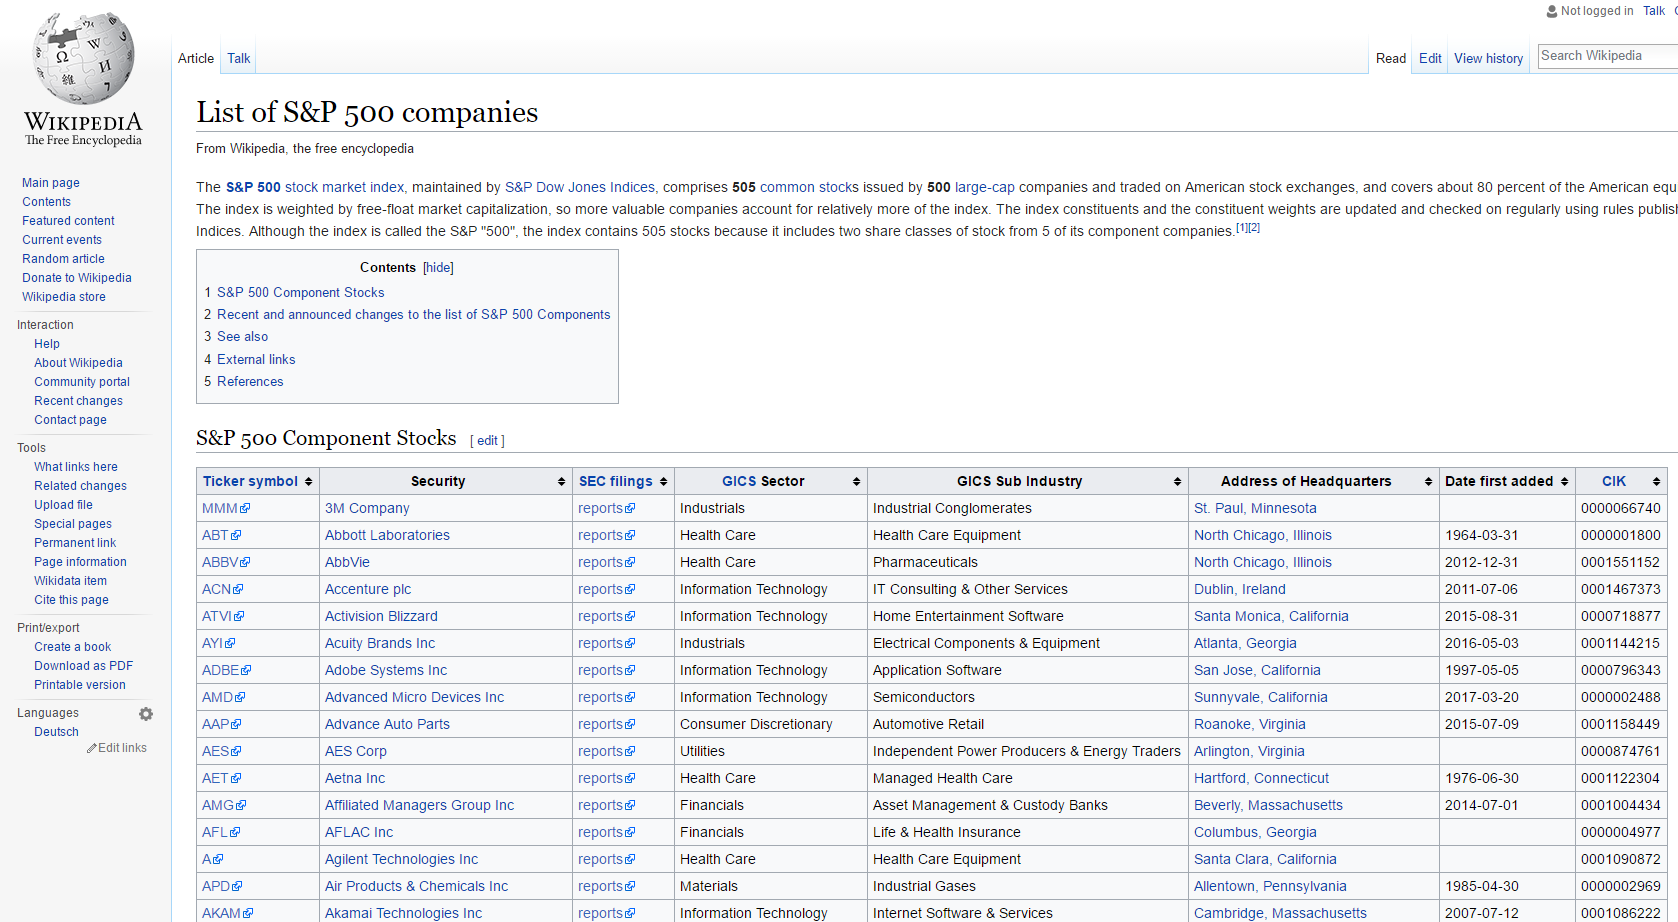
\includegraphics[width=0.75\linewidth]{figs/SP500-Wikipedia} 

}

\caption{Mirror of Wikipedia page on SP500 components}\label{fig:SP500-wikipedia}
\end{figure}

The information in this web page is constantly updated, and we can use
it to import information about the stocks belonging to the SP500 index.
Before delving into the R code, we need to understand how a webpage
works. In a nutshell, a webpage is nothing more than a lengthy
\emph{html} code interpreted by your browser. A numerical value or text
presented in the website can usually be found within the code. This code
has a particular structure with classes and formats. Every element of a
webpage has an address, called \emph{xpath} . In chrome and firefox
browsers, you can see the actual code of a webpage by using the mouse to
right-click any part of the webpage and selecting \emph{show source
code}.

The first step in webscraping is finding out where the information you
want is located. You can do that by right clicking in the specific
location of the number/text in the website and selecting \emph{inspect}.
This will open an extra window in the browser. Once you do that, right
click in the selection and chose \emph{copy} and \emph{copy xpath}. In
Figure \ref{fig:SP500-Wikipedia-webscraping}, we see a mirror of what
you should be seeing in your browser.

\begin{figure}[!htbp]

{\centering 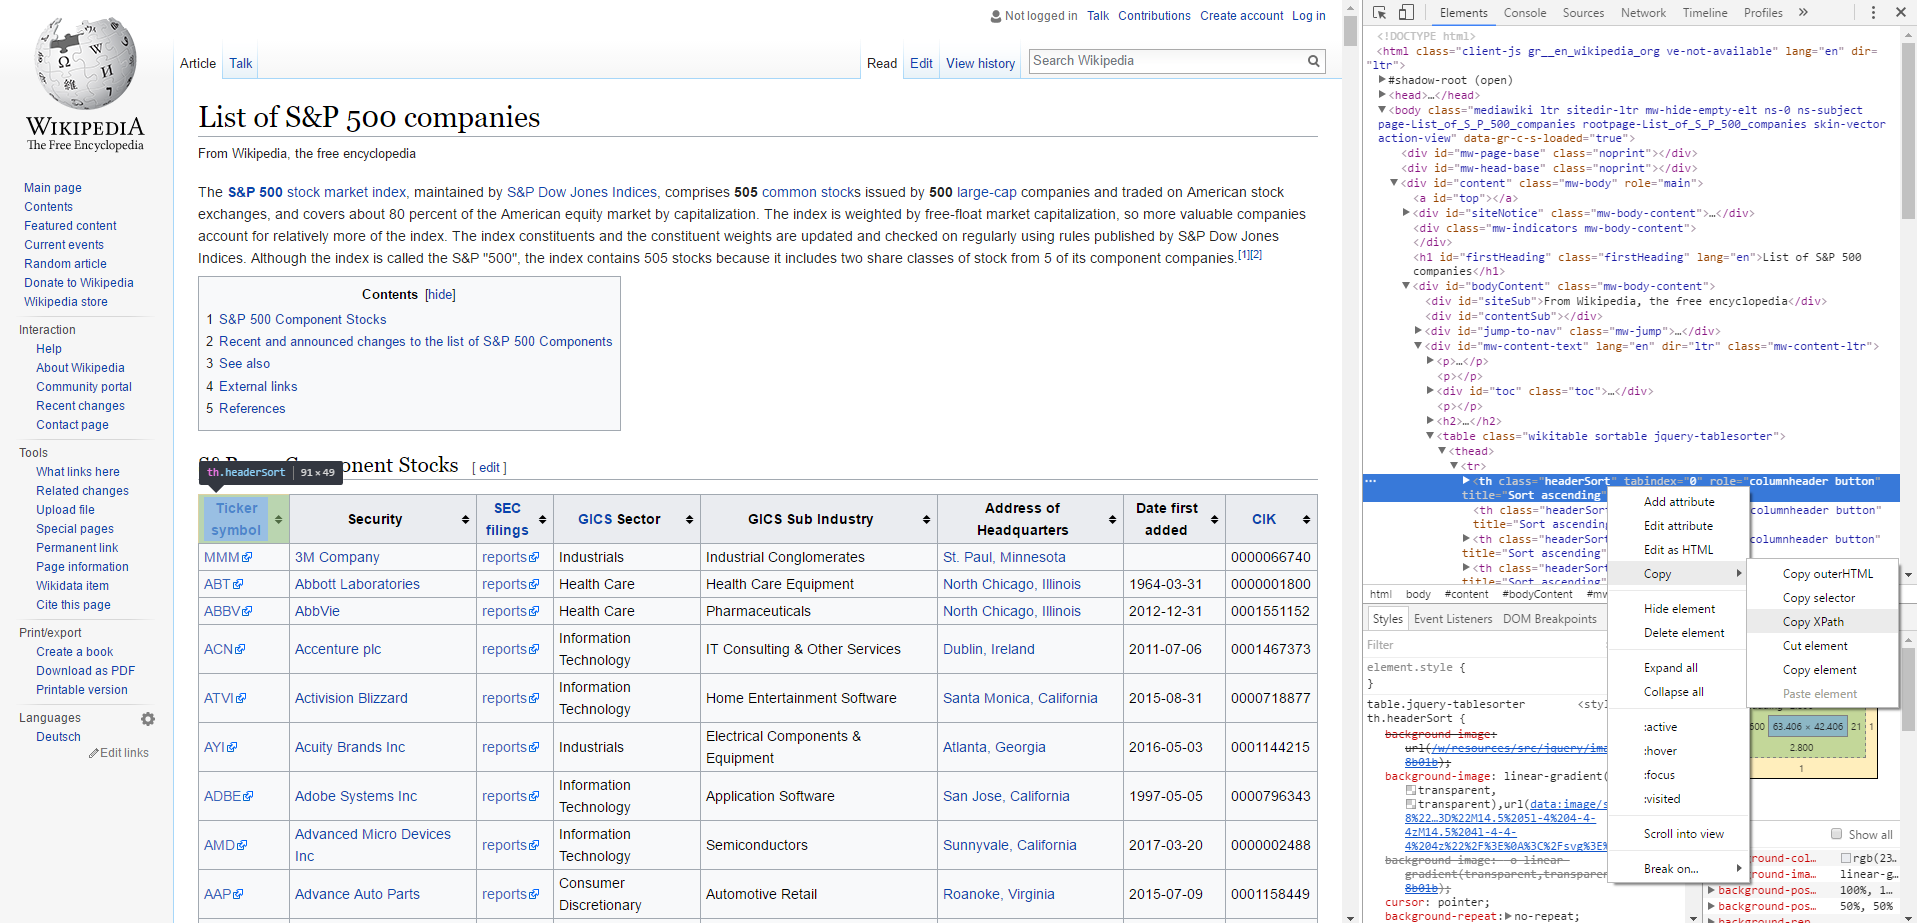
\includegraphics[width=0.75\linewidth]{figs/SP500-Wikipedia_webscraping} 

}

\caption{Finding xpath from website}\label{fig:SP500-Wikipedia-webscraping}
\end{figure}

In this case, the copied \emph{xpath} is:

\begin{Shaded}
\begin{Highlighting}[]
\StringTok{'//*[@id="mw-content-text"]/table[1]/thead/tr/th[2]'}
\end{Highlighting}
\end{Shaded}

This is the address of the header of the table. We can go to an upper
level and get all the content of the table, including header, rows, and
columns. This is equivalent to address
\texttt{//*{[}@id="mw-content-text"{]}/table{[}1{]}}.

Now that we have the location of what we want, let's load package
\texttt{rvest} \citep{rvest} and use functions \texttt{read\_html},
\texttt{html\_nodes} and \texttt{html\_table} to import the desired
table into R: \index{rvest} \index{rvest!read\_html}
\index{rvest!html\_nodes} \index{rvest!html\_table}

\begin{Shaded}
\begin{Highlighting}[]
\KeywordTok{library}\NormalTok{(rvest)}

\CommentTok{# set url and xpath}
\NormalTok{my.url <-}\StringTok{ 'https://en.wikipedia.org/wiki/List_of_S%26P_500_companies'}
\NormalTok{my.xpath <-}\StringTok{ '//*[@id="mw-content-text"]/table[1]'}

\CommentTok{# get nodes from html}
\NormalTok{out.nodes <-}\StringTok{ }\KeywordTok{html_nodes}\NormalTok{(}\KeywordTok{read_html}\NormalTok{(my.url),}
                        \DataTypeTok{xpath =}\NormalTok{ my.xpath)}

\CommentTok{# get table from nodes (each element in }
\CommentTok{# list is a table)}
\NormalTok{df.SP500Stocks <-}\StringTok{ }\KeywordTok{html_table}\NormalTok{(out.nodes)}

\CommentTok{# isolate it and print it}
\NormalTok{df.SP500Stocks <-}\StringTok{ }\NormalTok{df.SP500Stocks[[}\DecValTok{1}\NormalTok{]]}
\KeywordTok{print}\NormalTok{(}\KeywordTok{head}\NormalTok{(df.SP500Stocks))}
\end{Highlighting}
\end{Shaded}

\begin{verbatim}
##   Ticker symbol            Security SEC filings
## 1           MMM          3M Company     reports
## 2           ABT Abbott Laboratories     reports
## 3          ABBV         AbbVie Inc.     reports
## 4           ACN       Accenture plc     reports
## 5          ATVI Activision Blizzard     reports
## 6           AYI   Acuity Brands Inc     reports
##              GICS Sector                 GICS Sub Industry
## 1            Industrials          Industrial Conglomerates
## 2            Health Care             Health Care Equipment
## 3            Health Care                   Pharmaceuticals
## 4 Information Technology    IT Consulting & Other Services
## 5 Information Technology       Home Entertainment Software
## 6            Industrials Electrical Components & Equipment
##    Address of Headquarters Date first added     CIK
## 1      St. Paul, Minnesota                    66740
## 2  North Chicago, Illinois       1964-03-31    1800
## 3  North Chicago, Illinois       2012-12-31 1551152
## 4          Dublin, Ireland       2011-07-06 1467373
## 5 Santa Monica, California       2015-08-31  718877
## 6         Atlanta, Georgia       2016-05-03 1144215
\end{verbatim}

Object \texttt{df.SP500Stocks} contains a mirror of the data from the
Wikipedia website. The names of the columns require a bit of work, but
the data is intact and could be further used in a script.

\subsection{Scraping the Website of the Reserve Bank of
Australia}\label{scraping-the-website-of-the-reserve-bank-of-australia}

As another example of webscraping with R, let's import information from
the Reserve Bank of Australia. When accessed in 2017-03-24, its
\href{http://www.rba.gov.au/}{home page} mirrors Figure
\ref{fig:RBA-website}.

\begin{figure}[!htbp]

{\centering 
\includegraphics[width=0.75\linewidth]{figs/website_RBA-webscrapping} 

}

\caption{Website for the Reserve Bank of Australia}\label{fig:RBA-website}
\end{figure}

As you can see, the website offers financial information, such as news
and market rates. Let's assume we are interested in the information
about current cash/bank rate and inflation, right upper corner of the
webpage. The first step is finding out the \emph{xpath} of the
information we want. Using the procedure described in previous example,
we find out the address of both values, market rate and current
inflation:

\begin{Shaded}
\begin{Highlighting}[]
\NormalTok{my.xpath.inflation <-}\StringTok{ '//*[@id="content"]/section[1]/div/div[2]/p'}
\NormalTok{my.xpath.int.rate <-}\StringTok{ '//*[@id="content"]/section[1]/div/div[1]/p'}
\end{Highlighting}
\end{Shaded}

A difference from the previous example is we are not importing a table,
but a simple text from the website. For that, we use function
\texttt{html\_text} and not \texttt{html\_table}. The full code and its
output is presented next.

\begin{Shaded}
\begin{Highlighting}[]
\KeywordTok{library}\NormalTok{(rvest)}

\CommentTok{# set address of RBA}
\NormalTok{my.url <-}\StringTok{ 'http://www.rba.gov.au/'}

\CommentTok{# read html}
\NormalTok{html.code <-}\StringTok{ }\KeywordTok{read_html}\NormalTok{(my.url)}

\CommentTok{# set xpaths}
\NormalTok{my.xpath.inflation <-}\StringTok{ '//*[@id="content"]/section[1]/div/div[2]/p'}
\NormalTok{my.xpath.int.rate <-}\StringTok{ '//*[@id="content"]/section[1]/div/div[1]/p'}

\CommentTok{# get inflation from html}
\NormalTok{my.inflation <-}\StringTok{ }\KeywordTok{html_text}\NormalTok{(}\KeywordTok{html_nodes}\NormalTok{(html.code,}
                                     \DataTypeTok{xpath =}\NormalTok{ my.xpath.inflation ))}

\CommentTok{# get interest rate from html}
\NormalTok{my.int.rate <-}\StringTok{ }\KeywordTok{html_text}\NormalTok{(}\KeywordTok{html_nodes}\NormalTok{(}\DataTypeTok{x =}\NormalTok{ html.code,}
                                   \DataTypeTok{xpath =}\NormalTok{ my.xpath.int.rate ))}

\CommentTok{# print result}
\KeywordTok{cat}\NormalTok{(}\StringTok{"}\CharTok{\textbackslash{}n}\StringTok{Current inflation in AUS:"}\NormalTok{, my.inflation)}
\KeywordTok{cat}\NormalTok{(}\StringTok{"}\CharTok{\textbackslash{}n}\StringTok{Current interest rate AUS:"}\NormalTok{, my.int.rate)}
\end{Highlighting}
\end{Shaded}

\begin{verbatim}
## 
## Current inflation in AUS:  1.5%
\end{verbatim}

\begin{verbatim}
## 
## Current interest rate in AUS:  1.50%
\end{verbatim}

The use of \emph{Webscraping} techniques becomes a strong ally of the
researcher. They give you access to an immense amount of information
available on the web. However, each scenario of \emph{webscraping} is
particular. It is not always the case that you can import data directly
and easily as in the previous examples. Readers interested in this topic
should study the functionalities of packages \texttt{rvest}
\citep{rvest}, \texttt{XML} \citep{XML}, \texttt{RSelenium}
\citep{RSelenium} and \texttt{splashr}
(\href{https://github.com/hrbrmstr/splashr}{available in Github}). Each
one of these is best suited to particular webscraping problems.
\index{rvest} \index{XML} \index{RSelenium} \index{splashr}

\hypertarget{Figures}{\chapter{\texorpdfstring{Creating and Saving
Figures with
\texttt{ggplot2}}{Creating and Saving Figures with ggplot2}}\label{Figures}}

Using graphical resources in technical reports and academic documents is
widespread. Sometimes, this is simply what your audience expects. R has
built-in functions for creating figures, such as \texttt{plot} and
\texttt{hist}. Using the native plotting functions, however, is not
recommended. The customization of the graphic is not straightforward and
the options are limited. This deficiency was remedied by users. In 2005,
Hadley Wickham, author of many other packages featured in this book,
proposed a new way of structuring and creating figures in R, with a
package called \texttt{ggplot2} \citep{wickham2009ggplot2}. It provides
functions to generate graphics, structuring the process with an
accessible and intuitive \emph{layer} notation. This means graphics can
be customized quickly and easily. \index{ggplot2}

In this book, we will not go deep into \texttt{ggplot2} and all the
details of its capacity. We will show the main features of the package
for most situations of data analysis in finance. For advanced users who
want to know more about \texttt{ggplot2}, my advice is to consult the
author's own book \citep{wickham2009ggplot2}.

For most examples given here, we will work with the data available in
file \texttt{SP500-Stocks-WithRet.RData}. It contains daily closing
prices and returns data for all components of the SP500 index. This file
was created in chapter \ref{programming}.

First, let's load the data.

\begin{Shaded}
\begin{Highlighting}[]
\CommentTok{# set file and load data}
\NormalTok{my.f <-}\StringTok{ 'data/SP500-Stocks-WithRet.RData'}
\KeywordTok{load}\NormalTok{(my.f)}

\CommentTok{# print first 5 rows}
\KeywordTok{print}\NormalTok{(}\KeywordTok{head}\NormalTok{(my.df))}
\end{Highlighting}
\end{Shaded}

\begin{verbatim}
## # A tibble: 6 × 4
##   price.adjusted   ref.date ticker          ret
##            <dbl>     <date>  <chr>        <dbl>
## 1       68.72509 2010-01-05    MMM -0.006263503
## 2       69.69973 2010-01-06    MMM  0.014181794
## 3       69.74972 2010-01-07    MMM  0.000717162
## 4       70.24120 2010-01-08    MMM  0.007046423
## 5       69.95798 2010-01-11    MMM -0.004032220
## 6       70.01629 2010-01-12    MMM  0.000833529
\end{verbatim}

\section{Using Graphic Windows}\label{using-graphic-windows}

Before studying the use of \texttt{ggplot2}, we need to understand how
these images are handled within the RStudio platform. When a new figure
is created, as in \texttt{plot(1:20)}, it appears in the \emph{Plots}
panel (bottom right corner of RStudio). This panel, however, is small,
making it difficult to visualize the figure in standard monitors. You
can increase the panel's size manually, but this creates unnecessary
work, as you might need to resize it later to give space for other
panels.

A more intelligent approach to managing figures is to create an external
window in RStudio, so the graphic can be displayed and resized
independently of the main interface. To create a window, just use
command \texttt{x11()} before the line of code that creates the figure,
as in: \index{x11}

\begin{Shaded}
\begin{Highlighting}[]
\KeywordTok{x11}\NormalTok{()}
\KeywordTok{plot}\NormalTok{(}\DecValTok{1}\OperatorTok{:}\DecValTok{10}\NormalTok{)}
\end{Highlighting}
\end{Shaded}

The visual result in RStudio should be similar to Figure
\ref{fig:UseOfX11}.

\begin{figure}[!htbp]

{\centering 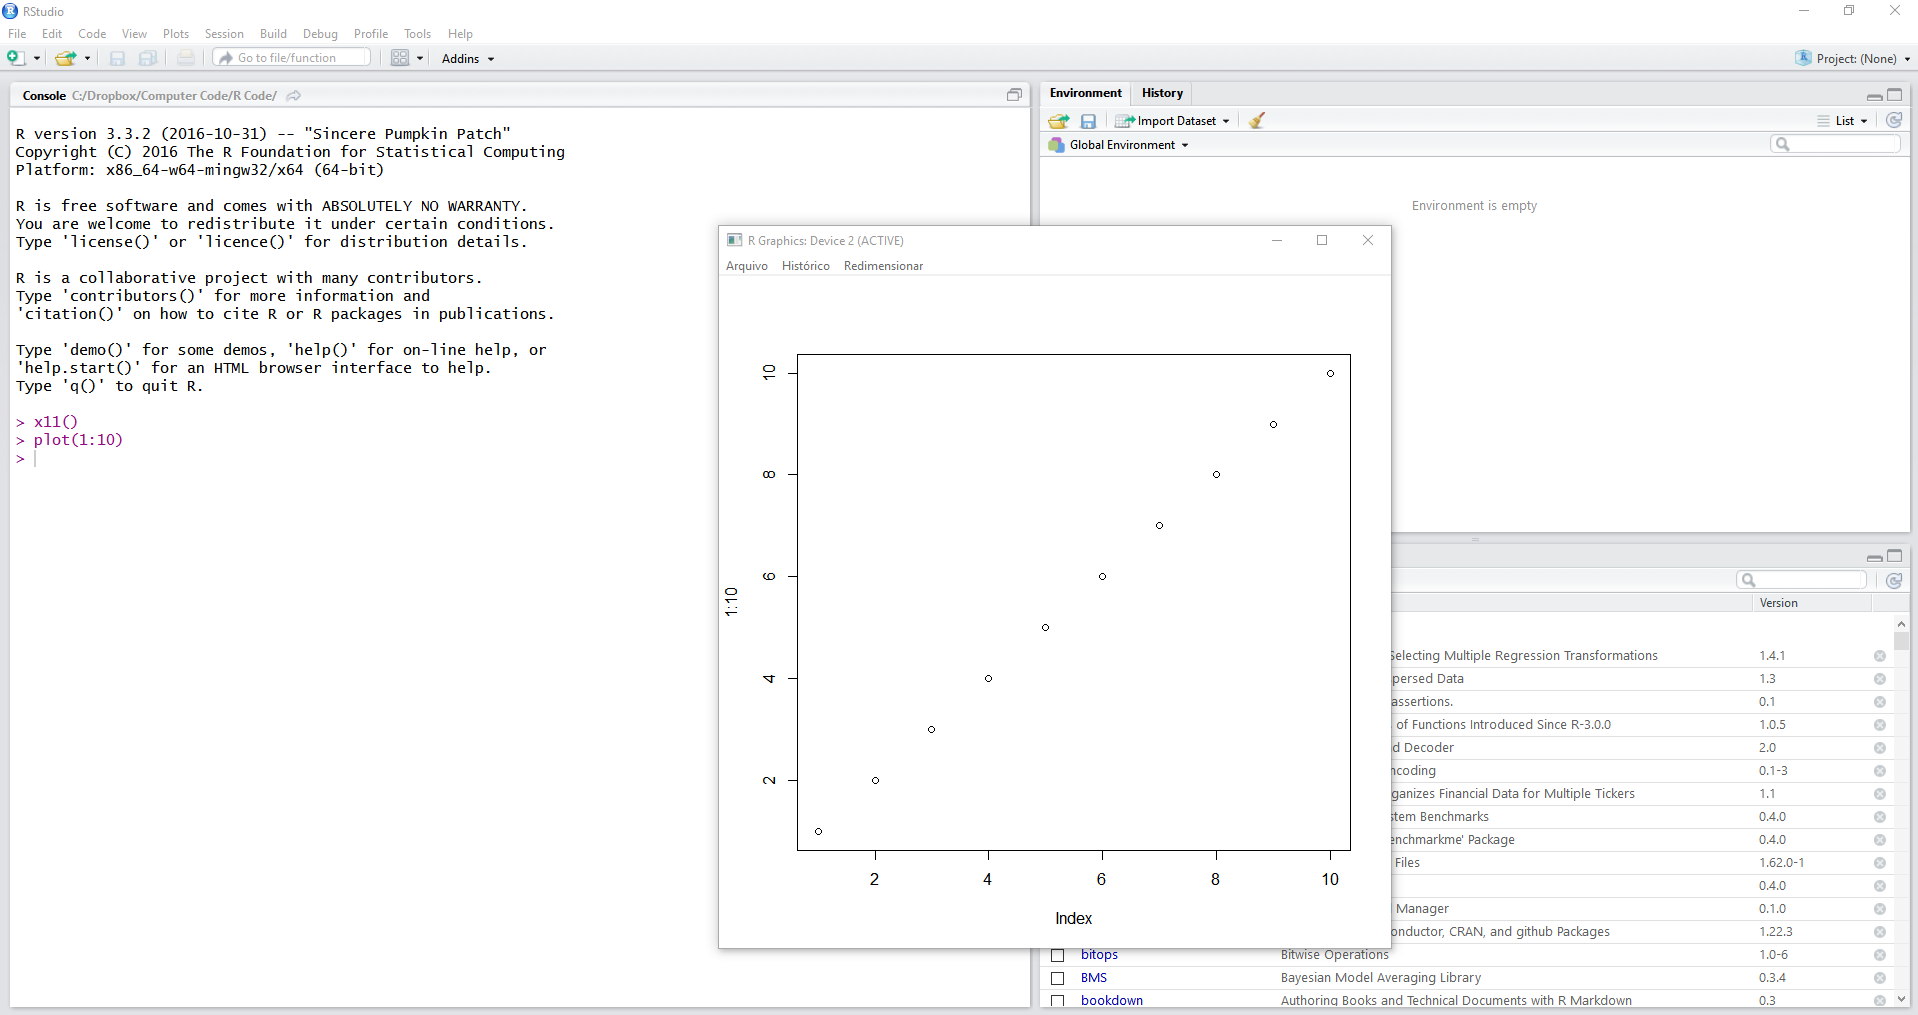
\includegraphics[width=1\linewidth]{figs/UseOfX11} 

}

\caption{Screen of RStudio with the use of command x11()}\label{fig:UseOfX11}
\end{figure}

Each call to \texttt{x11()} will create a new window. Therefore, we can
create various figures and allocate them in different windows, making it
easy to analyze each individually or together, side by side.

After creating so many windows, it is best to close them. You can use
\texttt{graphics.off} for that. This function, called with no argument,
as in \texttt{graphics.off()}, will close all opened windows. It is
common practice to use it in the beginning of a research script, so all
graphic windows are closed.

\section{\texorpdfstring{Creating Figures with Function
\texttt{qplot}}{Creating Figures with Function qplot}}\label{creating-figures-with-function-qplot}

Package \texttt{ggplot2} has an introductory function, called
\texttt{qplot} (\emph{quick plot}), that mimics the behaviour of the
native R function \texttt{plot}. To use it, all you need to know are the
points that define the horizontal axis (x), the points of the vertical
axis (y), and the geometric shape used in the plot.
\index{ggplot2!qplot}

To build a time series plot with the prices of stock \texttt{MMM}, we
use the following code:

\begin{Shaded}
\begin{Highlighting}[]
\KeywordTok{library}\NormalTok{(ggplot2)}

\CommentTok{# filter stock data}
\NormalTok{temp.df <-}\StringTok{ }\NormalTok{my.df[my.df}\OperatorTok{$}\NormalTok{ticker }\OperatorTok{==}\StringTok{ 'MMM'}\NormalTok{, ]}

\CommentTok{# plot its prices}
\KeywordTok{qplot}\NormalTok{(}\DataTypeTok{data =}\NormalTok{ temp.df, }
      \DataTypeTok{x =}\NormalTok{ ref.date, }
      \DataTypeTok{y =}\NormalTok{ price.adjusted, }
      \DataTypeTok{geom =} \StringTok{'line'}\NormalTok{)}
\end{Highlighting}
\end{Shaded}

\begin{center}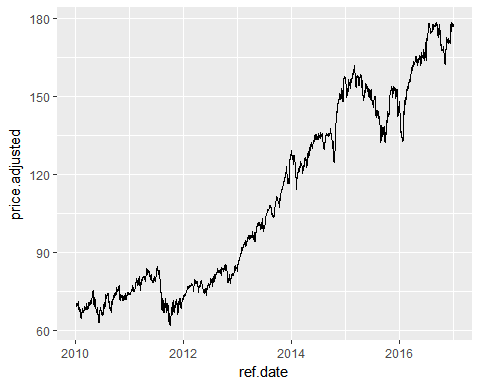
\includegraphics[width=0.6\linewidth]{ProcAnFinDataR_ed_1_files/figure-latex/unnamed-chunk-387-1} \end{center}

In the previous example, the name of the axis corresponds to the names
of the columns in \texttt{temp.df}. If we want to customize it for a
given text, we use arguments \texttt{xlab} and \texttt{ylab}:

\begin{Shaded}
\begin{Highlighting}[]
\KeywordTok{qplot}\NormalTok{(}\DataTypeTok{data =}\NormalTok{ temp.df, }
      \DataTypeTok{x =}\NormalTok{ ref.date, }
      \DataTypeTok{y =}\NormalTok{ price.adjusted, }
      \DataTypeTok{geom =} \StringTok{'line'}\NormalTok{, }
      \DataTypeTok{xlab =} \StringTok{'Dates'}\NormalTok{, }
      \DataTypeTok{ylab =} \StringTok{'Adjusted closing prices'}\NormalTok{)}
\end{Highlighting}
\end{Shaded}

\begin{center}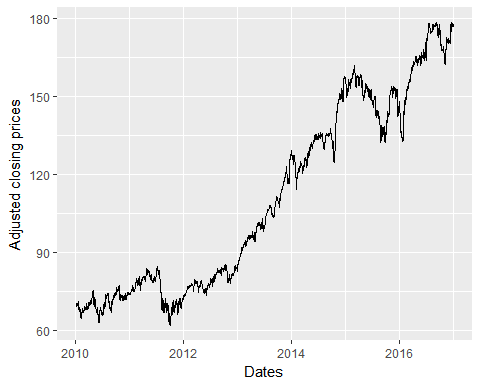
\includegraphics[width=0.6\linewidth]{ProcAnFinDataR_ed_1_files/figure-latex/unnamed-chunk-388-1} \end{center}

Notice how the horizontal axis of dates in the previous figures is
formatted to show only the years. It adapts automatically according to
the length of time in the plot. This only happened because the
\texttt{ref.date} column is correctly defined as a \texttt{Date} object.

\section{\texorpdfstring{Creating Figures with Function
\texttt{ggplot}}{Creating Figures with Function ggplot}}\label{ggplot}

Using function \texttt{qplot} is recommended when you want to create a
plot quickly for immediate viewing. This function has restrictions in
the way it works, making it more difficult to customize the output.The
recommended function to use in \texttt{ggplot2} is \texttt{ggplot}. It
uses a specific framework that allows a series of complex graphical
constructions. \index{ggplot2!ggplot}

Before presenting examples using \texttt{ggplot}, let's discuss the
philosophy behind how \texttt{ggplot} works. First, every figure has
horizontal and vertical coordinates. These points define where the
symbols or lines should be drawn. Second, we have a geometric shape
placed in the coordinates. It can be a circle, a point or a line, as in
the previous figures. We set the size and colour of these objects and,
finally, by combining all these elements, we create the full figure.

The distinction between the steps of creating a figure is important,
because it is precisely this way that \texttt{ggplot2} works. We make
choices for x, y, colour, and size based on data, and then chose the
desired format of the graphic. Everything works within each step, as if
we are drawing layers in the figure.

Look at the syntax of the following example that recreates the figure
previously created with \texttt{qplot}. \index{ggplot2!geom\_line}
\index{ggplot2!labs} \index{ggplot2!aes}

\begin{Shaded}
\begin{Highlighting}[]
\NormalTok{p <-}\StringTok{ }\KeywordTok{ggplot}\NormalTok{(}\DataTypeTok{data =}\NormalTok{ temp.df, }\KeywordTok{aes}\NormalTok{(}\DataTypeTok{x =}\NormalTok{ ref.date, }\DataTypeTok{y =}\NormalTok{ price.adjusted))}
\NormalTok{p <-}\StringTok{ }\NormalTok{p }\OperatorTok{+}\StringTok{ }\KeywordTok{geom_line}\NormalTok{()}
\NormalTok{p <-}\StringTok{ }\NormalTok{p }\OperatorTok{+}\StringTok{ }\KeywordTok{labs}\NormalTok{(}\DataTypeTok{x =} \StringTok{'Dates'}\NormalTok{, }\DataTypeTok{y =} \StringTok{'Adjusted closing prices'}\NormalTok{)}
\KeywordTok{print}\NormalTok{(p)}
\end{Highlighting}
\end{Shaded}

\begin{center}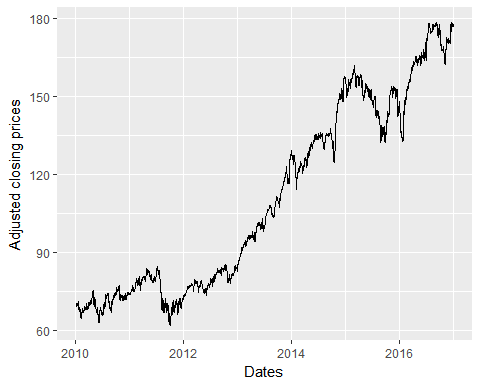
\includegraphics[width=0.6\linewidth]{ProcAnFinDataR_ed_1_files/figure-latex/unnamed-chunk-389-1} \end{center}

In using \texttt{ggplot}, it is always necessary to provide a
\texttt{dataframe}. If you want to create figures from atomic vectors,
you must allocate them to a \texttt{dataframe} first. After defining the
data, we use function \texttt{aes} to set the aesthetics of the graph
with the \emph{x} and \emph{y} coordinates. Here, we set the horizontal
axis using column \texttt{date} and the vertical axis as prices (column
\texttt{price.adjusted}). As we will soon see, it is possible to use
other information in \texttt{aes}, such as colour and shapes.

Once the data and axis are defined, we save it in object \texttt{p}.
This object registers the current information as new layers are added
with the \texttt{+} sign. The second line of the code,
\texttt{p\ \textless{}-\ p\ +\ geom\_line()}, defines the type of
figure. Here, we used function \texttt{geom\_lines}, which is a simple
line graph that connects the points. In \texttt{ggplot2}, the functions
that define the geometric type begins with \texttt{geom\_} character.
So, using the \emph{autocomplete} function of RStudio, you can see there
a lot of options. We can use \texttt{stringr} to find the list of
functions in \texttt{ggplot2}, version 2.2.1 (2017-05-03), that starts
with \texttt{geom\_}: \index{stringr!str\_sub}

\begin{Shaded}
\begin{Highlighting}[]
\KeywordTok{library}\NormalTok{(ggplot2)}
\KeywordTok{library}\NormalTok{(stringr)}

\CommentTok{# get names of functions in ggplot2}
\NormalTok{fcts <-}\StringTok{ }\KeywordTok{ls}\NormalTok{(}\StringTok{'package:ggplot2'}\NormalTok{)}

\CommentTok{# select those that starts with geom_}
\NormalTok{idx <-}\StringTok{ }\KeywordTok{str_sub}\NormalTok{(fcts, }\DecValTok{1}\NormalTok{, }\DecValTok{5}\NormalTok{) }\OperatorTok{==}\StringTok{ 'geom_'}
\NormalTok{fcts <-}\StringTok{ }\NormalTok{fcts[idx]}

\CommentTok{# print result}
\KeywordTok{print}\NormalTok{(fcts)}
\end{Highlighting}
\end{Shaded}

\begin{verbatim}
##  [1] "geom_abline"     "geom_area"       "geom_bar"       
##  [4] "geom_bin2d"      "geom_blank"      "geom_boxplot"   
##  [7] "geom_col"        "geom_contour"    "geom_count"     
## [10] "geom_crossbar"   "geom_curve"      "geom_density"   
## [13] "geom_density_2d" "geom_density2d"  "geom_dotplot"   
## [16] "geom_errorbar"   "geom_errorbarh"  "geom_freqpoly"  
## [19] "geom_hex"        "geom_histogram"  "geom_hline"     
## [22] "geom_jitter"     "geom_label"      "geom_line"      
## [25] "geom_linerange"  "geom_map"        "geom_path"      
## [28] "geom_point"      "geom_pointrange" "geom_polygon"   
## [31] "geom_qq"         "geom_quantile"   "geom_raster"    
## [34] "geom_rect"       "geom_ribbon"     "geom_rug"       
## [37] "geom_segment"    "geom_smooth"     "geom_spoke"     
## [40] "geom_step"       "geom_text"       "geom_tile"      
## [43] "geom_violin"     "geom_vline"
\end{verbatim}

As you can see, there are plenty of options. Package \texttt{ggplot2}
offers a significant quantity of geometrics shapes in creating figures.
Going back to our example, the third line of the code defines the name
of axis \emph{x} and \emph{y} with function \texttt{labs}. Finally, we
print the figure stored in \texttt{p} with function \texttt{print}. It
is important to highlight this modular approach in using
\texttt{ggplot}: each layer of the figure was created in a line of code.
For example, if we did not want to set the axes as \emph{Dates} and
\emph{Adjusted closing prices}, we can simply comment the line in the
script, as in:

\begin{Shaded}
\begin{Highlighting}[]
\NormalTok{p <-}\StringTok{ }\KeywordTok{ggplot}\NormalTok{(}\DataTypeTok{data =}\NormalTok{ temp.df, }\KeywordTok{aes}\NormalTok{(}\DataTypeTok{x =}\NormalTok{ ref.date, }\DataTypeTok{y =}\NormalTok{ price.adjusted))}
\NormalTok{p <-}\StringTok{ }\NormalTok{p }\OperatorTok{+}\StringTok{ }\KeywordTok{geom_line}\NormalTok{()}
\CommentTok{#p <- p + labs(x = 'Dates', y = 'Adjusted closing prices')}
\KeywordTok{print}\NormalTok{(p)}
\end{Highlighting}
\end{Shaded}

One of the great advantages of using \texttt{ggplot} is when creating
figures for different groups. Let's create a figure that shows, on the
same axis, prices of four stocks selected randomly. The first step is to
create a temporary \texttt{dataframe} that contains these stocks only.

\begin{Shaded}
\begin{Highlighting}[]
\CommentTok{# fix seed}
\KeywordTok{set.seed}\NormalTok{(}\DecValTok{10}\NormalTok{)}

\CommentTok{# select 4 stocks randomly}
\NormalTok{my.tickers <-}\StringTok{ }\KeywordTok{sample}\NormalTok{(}\KeywordTok{unique}\NormalTok{(my.df}\OperatorTok{$}\NormalTok{ticker), }\DecValTok{4}\NormalTok{)}

\CommentTok{# find all rows that contain the stocks}
\NormalTok{idx <-}\StringTok{ }\NormalTok{my.df}\OperatorTok{$}\NormalTok{ticker }\OperatorTok\StringTok{ }\NormalTok{my.tickers}

\CommentTok{# create temporary df}
\NormalTok{temp.df <-}\StringTok{ }\NormalTok{my.df[idx, ]}
\end{Highlighting}
\end{Shaded}

In this code, first, we set a random seed, so anyone can reproduce the
result. We use operator \texttt{\%in\%} to find out the rows of
\texttt{my.df} that contain data for the tickers in \texttt{my.tickers}.
It returns \texttt{TRUE} when any \emph{ticker} in \texttt{my.tickers}
is found and \texttt{FALSE} otherwise. After finding the rows, we create
a temporary \texttt{dataframe} that contains the data of the selected
stocks. Now, we create the figure with the following code:
\index{base!\%in\%}

\begin{Shaded}
\begin{Highlighting}[]
\NormalTok{p <-}\StringTok{ }\KeywordTok{ggplot}\NormalTok{(}\DataTypeTok{data =}\NormalTok{ temp.df, }\KeywordTok{aes}\NormalTok{(}\DataTypeTok{x =}\NormalTok{ ref.date, }
                                \DataTypeTok{y =}\NormalTok{ price.adjusted, }
                                \DataTypeTok{colour=}\NormalTok{ticker))}
\NormalTok{p <-}\StringTok{ }\NormalTok{p }\OperatorTok{+}\StringTok{ }\KeywordTok{geom_line}\NormalTok{()}
\NormalTok{p <-}\StringTok{ }\NormalTok{p }\OperatorTok{+}\StringTok{ }\KeywordTok{labs}\NormalTok{(}\DataTypeTok{x =} \StringTok{'Dates'}\NormalTok{, }\DataTypeTok{y =} \StringTok{'Adjusted closing prices'}\NormalTok{)}
\KeywordTok{print}\NormalTok{(p)}
\end{Highlighting}
\end{Shaded}

\begin{center}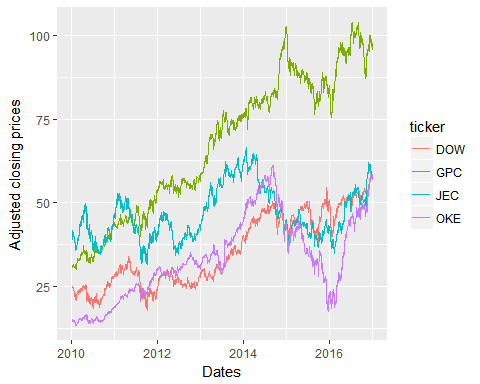
\includegraphics[width=0.6\linewidth]{ProcAnFinDataR_ed_1_files/figure-latex/unnamed-chunk-394-1} \end{center}

A difference from the previous examples is that we defined the colour of
the lines using argument \texttt{colour} in \texttt{aes}. Each line
colour is defined by the elements in column \texttt{ticker} of
\texttt{temp.df}. The actual choices of colour, e.g., red, blue, and so
on, is automatically defined by \texttt{ggplot}.

Now, let's use what we learned so far to create the current yield curve
of the US market. The yield curve is one of the standard plots in
finance, showing the market assessment of interest rates according to
different time horizons. In the following code, we will first download
the related data using package \texttt{ustyc}, structure and clean the
raw data, and plot the yields for the last available date in 2016 using
\texttt{ggplot2}. \index{yield curve figure}

\begin{Shaded}
\begin{Highlighting}[]
\KeywordTok{library}\NormalTok{(ustyc)}
\KeywordTok{library}\NormalTok{(tidyr)}
\KeywordTok{library}\NormalTok{(ggplot2)}
\KeywordTok{library}\NormalTok{(stringr)}

\CommentTok{# get yield curve}
\NormalTok{my.df.yc <-}\StringTok{ }\KeywordTok{getYieldCurve}\NormalTok{(}\DataTypeTok{year =} \DecValTok{2016}\NormalTok{)}\OperatorTok{$}\NormalTok{df}

\CommentTok{# set date.col}
\NormalTok{my.df.yc}\OperatorTok{$}\NormalTok{ref.date <-}\StringTok{ }\KeywordTok{as.Date}\NormalTok{(}\KeywordTok{rownames}\NormalTok{(my.df.yc))}

\CommentTok{# change to long format and convert to factor}
\NormalTok{my.df.yc <-}\StringTok{ }\KeywordTok{gather}\NormalTok{(}\DataTypeTok{data=}\NormalTok{my.df.yc, }\DataTypeTok{key =}\NormalTok{ref.date)}
\KeywordTok{names}\NormalTok{(my.df.yc) <-}\StringTok{ }\KeywordTok{c}\NormalTok{(}\StringTok{'ref.date'}\NormalTok{, }\StringTok{'maturity'}\NormalTok{, }\StringTok{'rate'}\NormalTok{)}
\NormalTok{my.df.yc}\OperatorTok{$}\NormalTok{maturity <-}\StringTok{ }\KeywordTok{as.factor}\NormalTok{(my.df.yc}\OperatorTok{$}\NormalTok{maturity)}

\CommentTok{# keep only longer term yields (names with YEAR)}
\NormalTok{idx <-}\StringTok{ }\KeywordTok{str_detect}\NormalTok{(my.df.yc}\OperatorTok{$}\NormalTok{maturity, }\StringTok{'YEAR'}\NormalTok{)}
\NormalTok{my.df.yc <-}\StringTok{ }\NormalTok{my.df.yc[idx, ]}

\CommentTok{# change name to year number with }
\CommentTok{# obs: regex ([0-9]+) extracts all numbers within a string}
\NormalTok{out <-}\StringTok{ }\KeywordTok{str_extract_all}\NormalTok{(}\DataTypeTok{string =}\NormalTok{ my.df.yc}\OperatorTok{$}\NormalTok{maturity,}
                       \DataTypeTok{pattern =} \StringTok{'([0-9]+)'}\NormalTok{)}
\NormalTok{my.df.yc}\OperatorTok{$}\NormalTok{maturity <-}\StringTok{ }\KeywordTok{as.numeric}\NormalTok{(out)}

\CommentTok{# keep only last date of each}
\NormalTok{last.date <-}\StringTok{ }\KeywordTok{max}\NormalTok{(my.df.yc}\OperatorTok{$}\NormalTok{ref.date)}
\NormalTok{my.df.yc.last.date <-}\StringTok{ }\NormalTok{my.df.yc[my.df.yc}\OperatorTok{$}\NormalTok{ref.date }\OperatorTok{==}\StringTok{ }\NormalTok{last.date, ]}

\CommentTok{# plot it!}
\NormalTok{p <-}\StringTok{ }\KeywordTok{ggplot}\NormalTok{(my.df.yc.last.date, }\KeywordTok{aes}\NormalTok{(}\DataTypeTok{x=}\NormalTok{maturity, }\DataTypeTok{y=}\NormalTok{rate))}
\NormalTok{p <-}\StringTok{ }\NormalTok{p }\OperatorTok{+}\StringTok{ }\KeywordTok{geom_point}\NormalTok{(}\DataTypeTok{size=}\DecValTok{2}\NormalTok{)}
\NormalTok{p <-}\StringTok{ }\NormalTok{p }\OperatorTok{+}\StringTok{ }\KeywordTok{geom_line}\NormalTok{(}\DataTypeTok{size=}\DecValTok{1}\NormalTok{)}
\NormalTok{p <-}\StringTok{ }\NormalTok{p }\OperatorTok{+}\StringTok{ }\KeywordTok{labs}\NormalTok{(}\DataTypeTok{x =} \StringTok{'Maturity (years)'}\NormalTok{, }
              \DataTypeTok{y=}\StringTok{'Yield Rate'}\NormalTok{,}
              \DataTypeTok{title =} \KeywordTok{paste0}\NormalTok{(}\StringTok{'US Yield Curve ('}\NormalTok{,last.date,}\StringTok{')'}\NormalTok{ ))}

\KeywordTok{print}\NormalTok{(p)}
\end{Highlighting}
\end{Shaded}

\begin{center}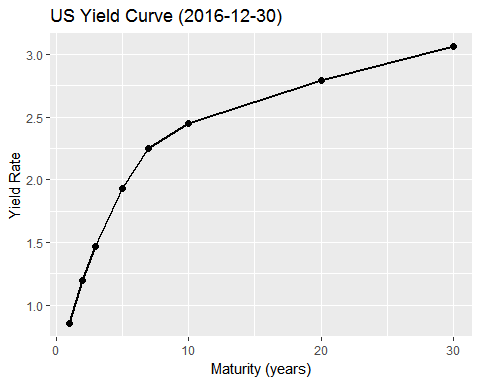
\includegraphics[width=0.6\linewidth]{ProcAnFinDataR_ed_1_files/figure-latex/unnamed-chunk-395-1} \end{center}

As expected, the current yield curve is upward rising, meaning the yield
rate increases with the maturity of the debt. As an extension of the
example, we can add some dynamic to the figure by using several dates.
Have a look in the following code, where we use five yield curves
covering the whole year of 2016.

\begin{Shaded}
\begin{Highlighting}[]
\CommentTok{# set number of periods }
\NormalTok{n.periods <-}\StringTok{ }\DecValTok{5}

\CommentTok{# set sequence of observations}
\NormalTok{my.seq <-}\StringTok{ }\KeywordTok{floor}\NormalTok{(}\KeywordTok{seq}\NormalTok{(}\DecValTok{1}\NormalTok{,}\KeywordTok{nrow}\NormalTok{(my.df.yc), }\DataTypeTok{length.out =}\NormalTok{ n.periods))}

\CommentTok{# get actual dates from sequence}
\NormalTok{my.dates <-}\StringTok{ }\NormalTok{my.df.yc}\OperatorTok{$}\NormalTok{ref.date[my.seq]}

\CommentTok{# find rows for dates in df}
\NormalTok{idx <-}\StringTok{ }\NormalTok{my.df.yc}\OperatorTok{$}\NormalTok{ref.date }\OperatorTok\StringTok{ }\NormalTok{my.dates}
\NormalTok{my.df.yc.periods <-}\StringTok{ }\NormalTok{my.df.yc[idx, ]}

\CommentTok{# plot it!}
\NormalTok{p <-}\StringTok{ }\KeywordTok{ggplot}\NormalTok{(my.df.yc.periods, }\KeywordTok{aes}\NormalTok{(}\DataTypeTok{x=}\NormalTok{maturity, }
                                  \DataTypeTok{y=}\NormalTok{rate, }
                                  \DataTypeTok{color=} \KeywordTok{factor}\NormalTok{(ref.date)))}
\NormalTok{p <-}\StringTok{ }\NormalTok{p }\OperatorTok{+}\StringTok{ }\KeywordTok{geom_point}\NormalTok{(}\DataTypeTok{size=}\DecValTok{2}\NormalTok{)}
\NormalTok{p <-}\StringTok{ }\NormalTok{p }\OperatorTok{+}\StringTok{ }\KeywordTok{geom_line}\NormalTok{(}\DataTypeTok{size=}\DecValTok{1}\NormalTok{)}
\NormalTok{p <-}\StringTok{ }\NormalTok{p }\OperatorTok{+}\StringTok{ }\KeywordTok{labs}\NormalTok{(}\DataTypeTok{x =} \StringTok{'Maturity (years)'}\NormalTok{, }
              \DataTypeTok{y=}\StringTok{'Yield Rate'}\NormalTok{,}
              \DataTypeTok{title =} \StringTok{'US Yield Curve'}\NormalTok{)}

\KeywordTok{print}\NormalTok{(p)}
\end{Highlighting}
\end{Shaded}

\begin{center}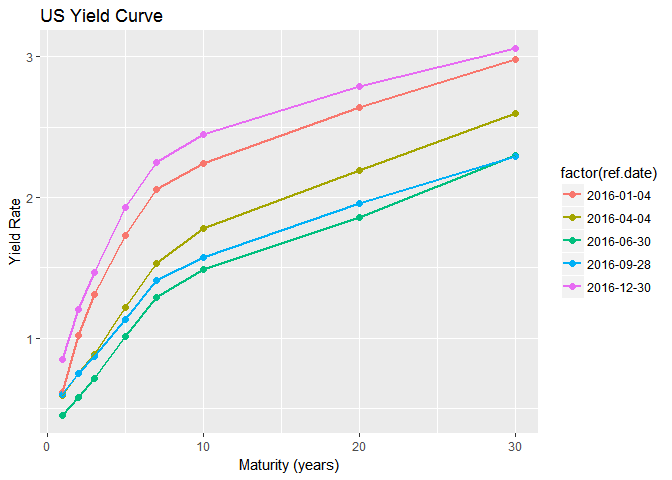
\includegraphics[width=0.6\linewidth]{ProcAnFinDataR_ed_1_files/figure-latex/unnamed-chunk-396-1} \end{center}

The US yield curve changed significantly in 2016. In empirical
applications, the information in the US yield curve can be used as a
benchmark for the calculation of cost of capital.

As another example of geometric shape in \texttt{ggplot}, let's create a
bar plot with the daily sharpe ratio, mean divided by standard deviation
of returns, for 10 assets from the database, ordered from high to low.
First, we need to calculate the sharpe ratio for each stock. This is
easily done with \texttt{dplyr}. Once the data is available, we use
\texttt{geom\_bar} to create the bar figure. Notice input \texttt{x} in
\texttt{aes} is set using \texttt{reorder(ticker,\ -sharpe.ratio)}. It
forces the horizontal axis to display descending values of sharpe ratio.

\begin{Shaded}
\begin{Highlighting}[]
\KeywordTok{library}\NormalTok{(dplyr)}
\CommentTok{# fix seed}
\KeywordTok{set.seed}\NormalTok{(}\DecValTok{10}\NormalTok{)}

\CommentTok{# select 10 stocks randomly}
\NormalTok{my.tickers <-}\StringTok{ }\KeywordTok{sample}\NormalTok{(}\KeywordTok{unique}\NormalTok{(my.df}\OperatorTok{$}\NormalTok{ticker), }\DecValTok{10}\NormalTok{)}

\CommentTok{# find all rows that contain the stocks}
\NormalTok{idx <-}\StringTok{ }\NormalTok{my.df}\OperatorTok{$}\NormalTok{ticker }\OperatorTok\StringTok{ }\NormalTok{my.tickers}

\CommentTok{# create temporary df}
\NormalTok{temp.df <-}\StringTok{ }\NormalTok{my.df[idx, ]}

\NormalTok{plot.df <-}\StringTok{ }\NormalTok{temp.df }\OperatorTok
\StringTok{  }\KeywordTok{group_by}\NormalTok{(ticker) }\OperatorTok
\StringTok{  }\KeywordTok{summarise}\NormalTok{(}\DataTypeTok{sharpe.ratio =} \KeywordTok{mean}\NormalTok{(ret)}\OperatorTok{/}\KeywordTok{sd}\NormalTok{(ret))}
  

\NormalTok{p <-}\StringTok{ }\KeywordTok{ggplot}\NormalTok{(}\DataTypeTok{data =}\NormalTok{ plot.df, }
            \KeywordTok{aes}\NormalTok{(}\DataTypeTok{x =} \KeywordTok{reorder}\NormalTok{(ticker, }\OperatorTok{-}\NormalTok{sharpe.ratio), }
            \DataTypeTok{y =}\NormalTok{ sharpe.ratio))}
\NormalTok{p <-}\StringTok{ }\NormalTok{p }\OperatorTok{+}\StringTok{ }\KeywordTok{geom_bar}\NormalTok{(}\DataTypeTok{stat =} \StringTok{'identity'}\NormalTok{)}
\NormalTok{p <-}\StringTok{ }\NormalTok{p }\OperatorTok{+}\StringTok{ }\KeywordTok{labs}\NormalTok{(}\DataTypeTok{x =} \StringTok{'Tickers'}\NormalTok{, }\DataTypeTok{y =} \StringTok{'Daily Sharpe Ratio'}\NormalTok{)}
\KeywordTok{print}\NormalTok{(p)}
\end{Highlighting}
\end{Shaded}

\begin{center}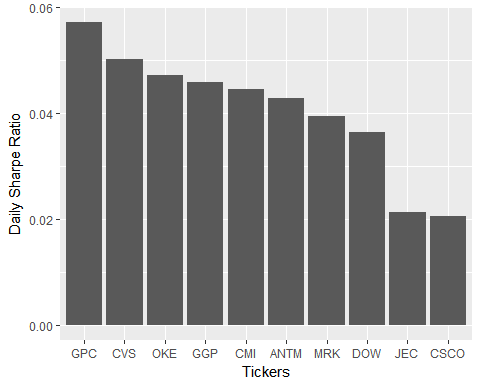
\includegraphics[width=0.6\linewidth]{ProcAnFinDataR_ed_1_files/figure-latex/unnamed-chunk-397-1} \end{center}

\subsection{Using Themes}\label{using-themes}

One way of customizing graphics in \texttt{ggplot2} is using themes. A
theme is a collection of options that defines the organization of the
figure, its points and line colours, notation of axis, background
colour, and several other features. Package \texttt{ggplot} has a
collection of functions for setting themes, and their name start with
text \emph{theme}. Next, we show the list of theme related functions in
\texttt{ggplot}, version 2.2.1 (2017-05-03).

\begin{Shaded}
\begin{Highlighting}[]
\KeywordTok{library}\NormalTok{(ggplot2)}
\KeywordTok{library}\NormalTok{(stringr)}

\CommentTok{# get all functions}
\NormalTok{fcts <-}\StringTok{ }\KeywordTok{ls}\NormalTok{(}\StringTok{'package:ggplot2'}\NormalTok{)}

\CommentTok{# find out those that start with theme_}
\NormalTok{idx <-}\StringTok{ }\KeywordTok{str_sub}\NormalTok{(fcts, }\DecValTok{1}\NormalTok{, }\DecValTok{6}\NormalTok{) }\OperatorTok{==}\StringTok{ 'theme_'}
\NormalTok{fcts <-}\StringTok{ }\NormalTok{fcts[idx]}

\CommentTok{# print result}
\KeywordTok{print}\NormalTok{(fcts)}
\end{Highlighting}
\end{Shaded}

\begin{verbatim}
##  [1] "theme_bw"       "theme_classic"  "theme_dark"    
##  [4] "theme_get"      "theme_gray"     "theme_grey"    
##  [7] "theme_light"    "theme_linedraw" "theme_minimal" 
## [10] "theme_replace"  "theme_set"      "theme_update"  
## [13] "theme_void"
\end{verbatim}

Let's try it with the theme of function \texttt{theme\_bw}. From the
manual: ``theme\_bw sets the classic dark-on-light ggplot2 theme. May
work better for presentations displayed with a projector.'' Let's look
at it visually. We need only to add a new line
\texttt{p\ \textless{}-\ p\ +\ theme\_bw()} in the previous code.
\index{ggplot2!theme\_bw}

\begin{Shaded}
\begin{Highlighting}[]
\NormalTok{p <-}\StringTok{ }\KeywordTok{ggplot}\NormalTok{(}\DataTypeTok{data =}\NormalTok{ temp.df, }\KeywordTok{aes}\NormalTok{(}\DataTypeTok{x =}\NormalTok{ ref.date, }
                                \DataTypeTok{y =}\NormalTok{ price.adjusted, }
                                \DataTypeTok{colour=}\NormalTok{ticker))}
\NormalTok{p <-}\StringTok{ }\NormalTok{p }\OperatorTok{+}\StringTok{ }\KeywordTok{geom_line}\NormalTok{()}
\NormalTok{p <-}\StringTok{ }\NormalTok{p }\OperatorTok{+}\StringTok{ }\KeywordTok{labs}\NormalTok{(}\DataTypeTok{x =} \StringTok{'Dates'}\NormalTok{, }\DataTypeTok{y =} \StringTok{'Adjusted closing prices'}\NormalTok{)}
\NormalTok{p <-}\StringTok{ }\NormalTok{p }\OperatorTok{+}\StringTok{ }\KeywordTok{theme_bw}\NormalTok{()}

\KeywordTok{print}\NormalTok{(p)}
\end{Highlighting}
\end{Shaded}

\begin{center}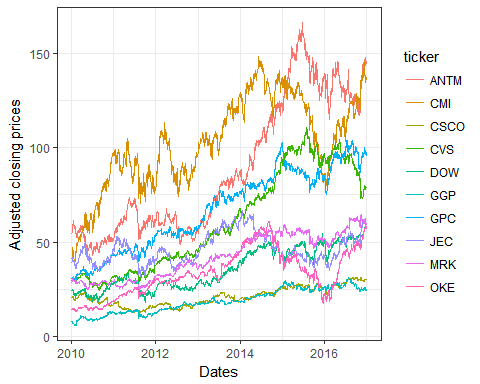
\includegraphics[width=0.6\linewidth]{ProcAnFinDataR_ed_1_files/figure-latex/unnamed-chunk-399-1} \end{center}

As you can see, the new theme was a white background and a frame box.
You can try other themes on your computer and see which one you like the
most. You can also create your own theme. Have a look at
\citet{wickham2009ggplot2} for instructions on this specific task.

In the previous example, notice how the structure of the figure has
changed, but not the colours of the lines. These selection of the
colours follows a cycle. When the whole sequence of colours ends, it
restarts. Sometimes, especially in the submission to scientific
journals, it is expected that all figures have a grey theme; they must
be in black and white. We can use function \texttt{scale\_colour\_grey}
to set a colour cycle between white and black in our previous figure:
\index{ggplot2!scale\_colour\_grey}

\begin{Shaded}
\begin{Highlighting}[]
\NormalTok{p <-}\StringTok{ }\NormalTok{p }\OperatorTok{+}\StringTok{ }\KeywordTok{scale_colour_grey}\NormalTok{(}\DataTypeTok{start =} \FloatTok{0.0}\NormalTok{, }\DataTypeTok{end =} \FloatTok{0.6}\NormalTok{)}
\KeywordTok{print}\NormalTok{(p)  }
\end{Highlighting}
\end{Shaded}

\begin{center}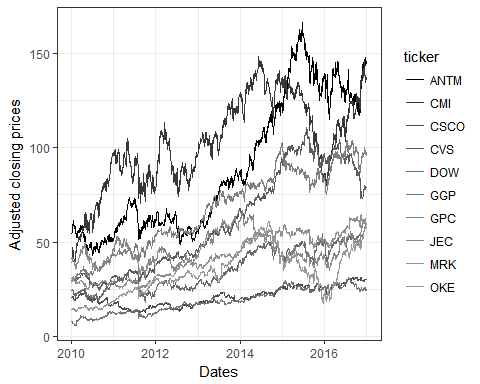
\includegraphics[width=0.6\linewidth]{ProcAnFinDataR_ed_1_files/figure-latex/unnamed-chunk-400-1} \end{center}

The lines of the plot are now in grey. The inputs \texttt{start} and
\texttt{end} at \texttt{scale\_color\_grey} set the minimum and maximum
of ``whiteness''. So, never use \texttt{end=1} with a white background.
Otherwise, some lines will will not be visible.

\subsection{\texorpdfstring{Creating Panels with
\texttt{facet\_wrap}}{Creating Panels with facet\_wrap}}\label{creating-panels-with-facet_wrap}

Another possibility in creating graphics for different groups is to use
panels. It allocates each group in a different part of the figure. When
placed side by side and with the same axis, the visual comparison is
straightforward.

Facets are possible with function \texttt{facet\_wrap}, which takes as
input a formula containing the name of a column with groups that will
define each panel. In the following example, we use \texttt{facet\_wrap}
with option \texttt{facets\ =\ \textasciitilde{}\ ticker} to create a
panel of prices for four selected assets. \index{ggplot2!facet\_wrap}

\begin{Shaded}
\begin{Highlighting}[]
\KeywordTok{library}\NormalTok{(dplyr)}
\CommentTok{# fix seed}
\KeywordTok{set.seed}\NormalTok{(}\DecValTok{20}\NormalTok{)}

\CommentTok{# select 4 stocks randomly}
\NormalTok{my.tickers <-}\StringTok{ }\KeywordTok{sample}\NormalTok{(}\KeywordTok{unique}\NormalTok{(my.df}\OperatorTok{$}\NormalTok{ticker), }\DecValTok{4}\NormalTok{)}

\NormalTok{p <-}\StringTok{ }\NormalTok{my.df }\OperatorTok
\StringTok{  }\KeywordTok{filter}\NormalTok{(ticker }\OperatorTok\StringTok{ }\NormalTok{my.tickers) }\OperatorTok
\StringTok{  }\KeywordTok{ggplot}\NormalTok{(}\KeywordTok{aes}\NormalTok{(}\DataTypeTok{x =}\NormalTok{ ref.date, }\DataTypeTok{y =}\NormalTok{ price.adjusted)) }\OperatorTok{+}\StringTok{ }
\StringTok{  }\KeywordTok{geom_line}\NormalTok{() }\OperatorTok{+}\StringTok{ }
\StringTok{  }\KeywordTok{labs}\NormalTok{(}\DataTypeTok{x =} \StringTok{'Date'}\NormalTok{, }
       \DataTypeTok{y =} \StringTok{'Adjusted closing prices'}\NormalTok{) }\OperatorTok{+}\StringTok{ }
\StringTok{  }\KeywordTok{facet_wrap}\NormalTok{(}\DataTypeTok{facets =} \OperatorTok{~}\NormalTok{ticker)}
    
\KeywordTok{print}\NormalTok{(p)}
\end{Highlighting}
\end{Shaded}

\begin{center}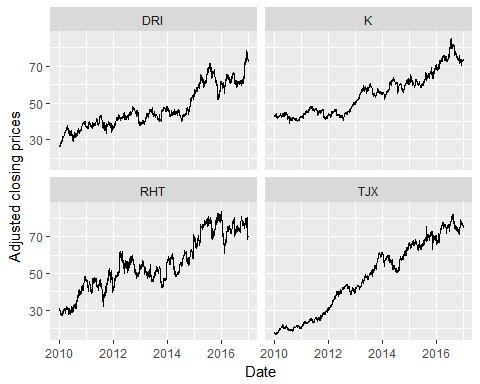
\includegraphics[width=0.6\linewidth]{ProcAnFinDataR_ed_1_files/figure-latex/unnamed-chunk-401-1} \end{center}

Using panels is recommended when the data of the groups are similar and
tend to agglomerate. This makes it difficult to analyze the differences
between the groups in a single graphic. This is the case of stock
returns of different assets. Consider the following example, where we
create a panel for the returns of four randomly selected shares.

\begin{Shaded}
\begin{Highlighting}[]
\CommentTok{# fix seed}
\KeywordTok{set.seed}\NormalTok{(}\DecValTok{25}\NormalTok{)}

\CommentTok{# select 4 stocks randomly}
\NormalTok{my.tickers <-}\StringTok{ }\KeywordTok{sample}\NormalTok{(}\KeywordTok{unique}\NormalTok{(my.df}\OperatorTok{$}\NormalTok{ticker), }\DecValTok{4}\NormalTok{)}

\NormalTok{p <-}\StringTok{ }\NormalTok{my.df }\OperatorTok
\StringTok{  }\KeywordTok{filter}\NormalTok{(ticker }\OperatorTok\StringTok{ }\NormalTok{my.tickers) }\OperatorTok
\StringTok{  }\KeywordTok{ggplot}\NormalTok{(}\KeywordTok{aes}\NormalTok{(}\DataTypeTok{x =}\NormalTok{ ref.date, }\DataTypeTok{y =}\NormalTok{ ret)) }\OperatorTok{+}\StringTok{ }
\StringTok{  }\KeywordTok{geom_line}\NormalTok{(}\DataTypeTok{size=}\DecValTok{1}\NormalTok{) }\OperatorTok{+}\StringTok{ }
\StringTok{  }\KeywordTok{labs}\NormalTok{(}\DataTypeTok{x =} \StringTok{'Date'}\NormalTok{, }
       \DataTypeTok{y =} \StringTok{'Returns'}\NormalTok{) }\OperatorTok{+}\StringTok{   }
\StringTok{  }\KeywordTok{facet_wrap}\NormalTok{(}\DataTypeTok{facets =} \OperatorTok{~}\NormalTok{ticker)}
    
\KeywordTok{print}\NormalTok{(p)}
\end{Highlighting}
\end{Shaded}

\begin{center}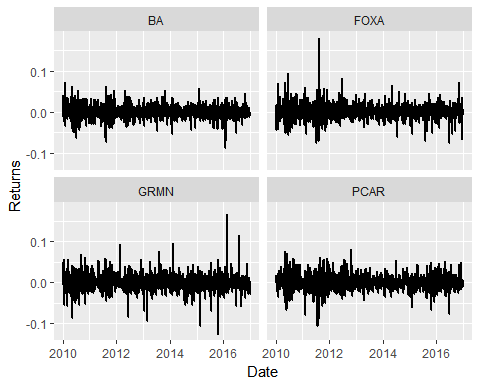
\includegraphics[width=0.6\linewidth]{ProcAnFinDataR_ed_1_files/figure-latex/unnamed-chunk-402-1} \end{center}

Notice how the vertical axis of the panels is fixed for all stocks,
facilitating the visual analysis. We can also set the scales free by
using option \texttt{scales=\textquotesingle{}free\textquotesingle{}} in
\texttt{facet\_wrap}:

\begin{Shaded}
\begin{Highlighting}[]
\NormalTok{p <-}\StringTok{ }\NormalTok{p }\OperatorTok{+}\StringTok{ }\KeywordTok{facet_wrap}\NormalTok{(}\DataTypeTok{facets =} \OperatorTok{~}\NormalTok{ticker, }\DataTypeTok{scales =} \StringTok{'free'}\NormalTok{)}
    
\KeywordTok{print}\NormalTok{(p)}
\end{Highlighting}
\end{Shaded}

\begin{center}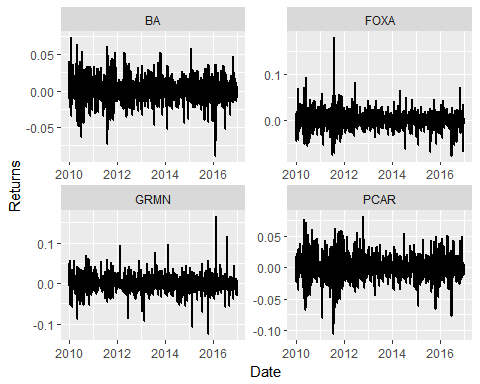
\includegraphics[width=0.6\linewidth]{ProcAnFinDataR_ed_1_files/figure-latex/unnamed-chunk-403-1} \end{center}

\section{Using Pipelines for Data Analysis and
Figures}\label{using-pipelines-for-data-analysis-and-figures}

Another great thing about \texttt{ggplot2} is you can use the pipeline
operator and write a code where data processing and plotting are
integrated. Look at the next example, where we plot the average return
and standard deviation of all stocks from the dataset available in
\texttt{my.df}.

\begin{Shaded}
\begin{Highlighting}[]
\KeywordTok{library}\NormalTok{(dplyr)}
\KeywordTok{library}\NormalTok{(ggplot2)}

\CommentTok{# calculated mean and sd of returns, plot result}
\NormalTok{p <-}\StringTok{ }\NormalTok{my.df }\OperatorTok
\StringTok{  }\KeywordTok{group_by}\NormalTok{(ticker) }\OperatorTok
\StringTok{  }\KeywordTok{summarise}\NormalTok{(}\DataTypeTok{mean.ret =} \KeywordTok{mean}\NormalTok{(ret),}
            \DataTypeTok{std.ret =} \KeywordTok{sd}\NormalTok{(ret)) }\OperatorTok
\StringTok{  }\KeywordTok{ggplot}\NormalTok{(}\KeywordTok{aes}\NormalTok{(}\DataTypeTok{x =}\NormalTok{ std.ret, }\DataTypeTok{y =}\NormalTok{ mean.ret)) }\OperatorTok{+}
\StringTok{  }\KeywordTok{geom_point}\NormalTok{() }\OperatorTok{+}\StringTok{ }
\StringTok{  }\KeywordTok{labs}\NormalTok{(}\DataTypeTok{x =} \StringTok{'Standard deviation of returns'}\NormalTok{, }
       \DataTypeTok{y =} \StringTok{'Average Returns'}\NormalTok{)}


\KeywordTok{print}\NormalTok{(p)}
\end{Highlighting}
\end{Shaded}

\begin{center}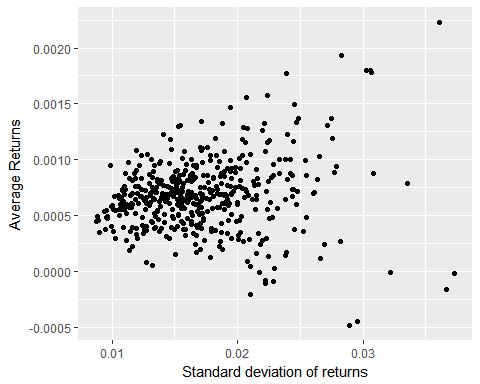
\includegraphics[width=0.6\linewidth]{ProcAnFinDataR_ed_1_files/figure-latex/unnamed-chunk-404-1} \end{center}

Notice how the previous code is self-contained, easy to read, and
elegant. It goes from raw data to the plot, with no object created in
the intermediate steps. Anyone can clearly see the steps taken to build
the plot. Modifications in the data processing stage are also
straightforward. One detail about using pipelines with \texttt{ggplot}
is the steps in the plot creation are incremented with the \texttt{+}
sign, not \texttt{\%\textgreater{}\%}. From this section on, we will use
the pipeline notation to simplify the code, whenever possible.

We only scratched the surface of \texttt{ggplot2}. Many other aspects of
the resulting figure can be controlled. Users with a specific need may
consult the manual or the main reference of the package,
\citet{wickham2009ggplot2}. Forums and \emph{mailing lists} are also a
great source of information.

\section{Creating Statistical
Graphics}\label{creating-statistical-graphics}

Package \texttt{ggplot} has several options for creating graphs with
statistical content. This includes histograms, \emph{boxplot} graphics,
QQ plots, and more.

\subsection{Creating Histograms}\label{creating-histograms}

A histogram shows the empirical distribution of the data. We can easily
create them with \texttt{ggplot} and function \texttt{geom\_histogram}.
An example is given in the following code, where we generate a histogram
for all returns found in \texttt{my.df}.

\begin{Shaded}
\begin{Highlighting}[]
\NormalTok{p <-}\StringTok{ }\KeywordTok{ggplot}\NormalTok{(}\DataTypeTok{data =}\NormalTok{ my.df, }\KeywordTok{aes}\NormalTok{(}\DataTypeTok{x =}\NormalTok{ ret))}
\NormalTok{p <-}\StringTok{ }\NormalTok{p }\OperatorTok{+}\StringTok{ }\KeywordTok{geom_histogram}\NormalTok{(}\DataTypeTok{bins =} \DecValTok{25}\NormalTok{)}
  
\KeywordTok{print}\NormalTok{(p)}
\end{Highlighting}
\end{Shaded}

\begin{center}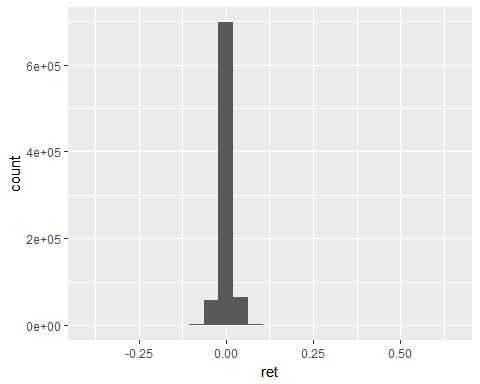
\includegraphics[width=0.6\linewidth]{ProcAnFinDataR_ed_1_files/figure-latex/unnamed-chunk-405-1} \end{center}

Here, we only need to define the \emph{x} value, without the \emph{y}.
The size of the intervals in the histogram is defined by input
\texttt{bins}.

We can also use groups and facets as we did for point and line plots.
Have a look.

\begin{Shaded}
\begin{Highlighting}[]
\CommentTok{# fix seed}
\KeywordTok{set.seed}\NormalTok{(}\DecValTok{30}\NormalTok{)}

\CommentTok{# select 4 stocks randomly}
\NormalTok{my.tickers <-}\StringTok{ }\KeywordTok{sample}\NormalTok{(}\KeywordTok{unique}\NormalTok{(my.df}\OperatorTok{$}\NormalTok{ticker), }\DecValTok{4}\NormalTok{)}

\NormalTok{p <-}\StringTok{ }\NormalTok{my.df }\OperatorTok
\StringTok{  }\KeywordTok{filter}\NormalTok{(ticker }\OperatorTok\StringTok{ }\NormalTok{my.tickers) }\OperatorTok
\StringTok{  }\KeywordTok{ggplot}\NormalTok{(}\KeywordTok{aes}\NormalTok{(}\DataTypeTok{x =}\NormalTok{ ret)) }\OperatorTok{+}\StringTok{ }
\StringTok{  }\KeywordTok{geom_histogram}\NormalTok{(}\DataTypeTok{bins =} \DecValTok{50}\NormalTok{) }\OperatorTok{+}
\StringTok{  }\KeywordTok{facet_wrap}\NormalTok{(}\DataTypeTok{facets =} \OperatorTok{~}\NormalTok{ticker)}
  
\KeywordTok{print}\NormalTok{(p)}
\end{Highlighting}
\end{Shaded}

\begin{center}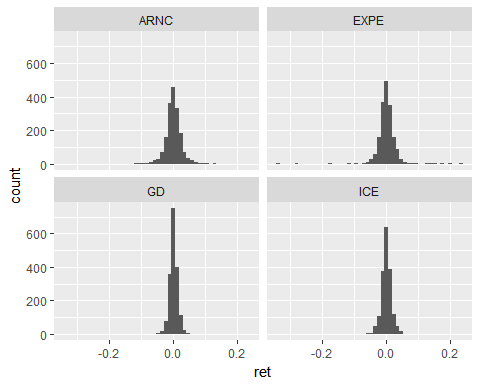
\includegraphics[width=0.6\linewidth]{ProcAnFinDataR_ed_1_files/figure-latex/unnamed-chunk-406-1} \end{center}

A histogram with the empirical densities of the data can be created
using function \texttt{geom\_density}. While histograms built with
\texttt{geom\_histogram} count the number of times the data is located
within an interval, a density histogram uses the relative frequency and
interpolates the values, resulting in a more visually appealing
representation of a distribution. See an example next.

\begin{Shaded}
\begin{Highlighting}[]
\NormalTok{p <-}\StringTok{ }\NormalTok{my.df }\OperatorTok
\StringTok{  }\KeywordTok{filter}\NormalTok{(ticker }\OperatorTok\StringTok{ }\NormalTok{my.tickers) }\OperatorTok
\StringTok{  }\KeywordTok{ggplot}\NormalTok{(}\KeywordTok{aes}\NormalTok{(}\DataTypeTok{x =}\NormalTok{ ret)) }\OperatorTok{+}\StringTok{ }
\StringTok{  }\KeywordTok{geom_density}\NormalTok{() }\OperatorTok{+}\StringTok{ }
\StringTok{  }\KeywordTok{facet_wrap}\NormalTok{(}\DataTypeTok{facets =} \OperatorTok{~}\NormalTok{ticker)}
  
\KeywordTok{print}\NormalTok{(p)}
\end{Highlighting}
\end{Shaded}

\begin{center}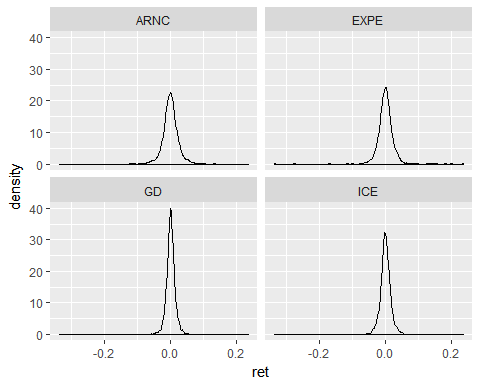
\includegraphics[width=0.6\linewidth]{ProcAnFinDataR_ed_1_files/figure-latex/unnamed-chunk-407-1} \end{center}

The previous figure allows a clear visual comparison of the differences
between the distributions of returns of the different stocks.

\subsection{\texorpdfstring{Creating \emph{boxplot}
Figures}{Creating boxplot Figures}}\label{creating-boxplot-figures}

Figures of type \emph{boxplot} (or box and whisker diagram) show the
distribution of a variable conditional on some category or group. Using
the median, maximum, minimum, and quartiles of the data, this
statistical display highlights the distribution of a variable in a
specific visual pattern. We can easily create them with \texttt{ggplot}.
See an example next, where we show the price distribution of four
randomly selected stocks.

\begin{Shaded}
\begin{Highlighting}[]
\CommentTok{# fix seed}
\KeywordTok{set.seed}\NormalTok{(}\DecValTok{35}\NormalTok{)}

\CommentTok{# select 4 stocks randomly}
\NormalTok{my.tickers <-}\StringTok{ }\KeywordTok{sample}\NormalTok{(}\KeywordTok{unique}\NormalTok{(my.df}\OperatorTok{$}\NormalTok{ticker), }\DecValTok{4}\NormalTok{)}

\NormalTok{p <-}\StringTok{ }\NormalTok{my.df }\OperatorTok
\StringTok{  }\KeywordTok{filter}\NormalTok{(ticker }\OperatorTok\StringTok{ }\NormalTok{my.tickers) }\OperatorTok
\StringTok{  }\KeywordTok{ggplot}\NormalTok{(}\KeywordTok{aes}\NormalTok{(}\DataTypeTok{x =}\NormalTok{ ticker, }\DataTypeTok{y =}\NormalTok{ price.adjusted)) }\OperatorTok{+}\StringTok{ }
\StringTok{  }\KeywordTok{geom_boxplot}\NormalTok{()}
  
\KeywordTok{print}\NormalTok{(p)}
\end{Highlighting}
\end{Shaded}

\begin{center}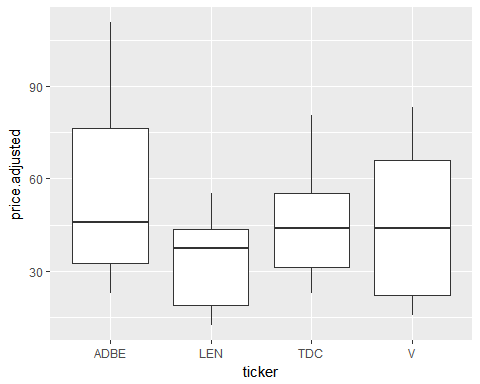
\includegraphics[width=0.6\linewidth]{ProcAnFinDataR_ed_1_files/figure-latex/unnamed-chunk-408-1} \end{center}

As we can see from the previous figure, the stocks have different
distributions for their prices. The middle line defines the median
value, while the upper and lower lines of the box define the first and
third quartile.

\subsection{\texorpdfstring{Creating \emph{QQ}
Plots}{Creating QQ Plots}}\label{creating-qq-plots}

QQ plots show a comparison between the distribution of a variable and a
theoretical distribution, such as the Normal. It is a scatter plot
between cumulative distributions. The closest to a straight line, the
more similar is the empirical distribution to the theoretical.

Let's try an example with some simulated data.

\begin{Shaded}
\begin{Highlighting}[]
\CommentTok{# fix seed}
\KeywordTok{set.seed}\NormalTok{(}\DecValTok{40}\NormalTok{)}

\NormalTok{N=}\DecValTok{1000}
\NormalTok{my.mean <-}\StringTok{ }\DecValTok{10}
\NormalTok{my.sd <-}\StringTok{ }\DecValTok{2}

\NormalTok{temp.df <-}\StringTok{ }\KeywordTok{data.frame}\NormalTok{(}\DataTypeTok{y=}\KeywordTok{rnorm}\NormalTok{(}\DataTypeTok{n =}\NormalTok{ N, }\DataTypeTok{mean =}\NormalTok{ my.mean, }\DataTypeTok{sd =}\NormalTok{ my.sd))}

\NormalTok{p <-}\StringTok{ }\KeywordTok{ggplot}\NormalTok{(}\DataTypeTok{data =}\NormalTok{ temp.df, }\KeywordTok{aes}\NormalTok{(}\DataTypeTok{sample =}\NormalTok{ y)) }
\CommentTok{#p <- p + labs(title = 'QQ plot for simulated data')}
\NormalTok{p <-}\StringTok{ }\NormalTok{p }\OperatorTok{+}\StringTok{ }\KeywordTok{geom_qq}\NormalTok{(}\DataTypeTok{distribution =}\NormalTok{ qnorm, }
                 \DataTypeTok{dparams =} \KeywordTok{c}\NormalTok{(}\DataTypeTok{mean=}\NormalTok{my.mean, }\DataTypeTok{sd=}\NormalTok{my.sd))}
  
\KeywordTok{print}\NormalTok{(p)}
\end{Highlighting}
\end{Shaded}

\begin{center}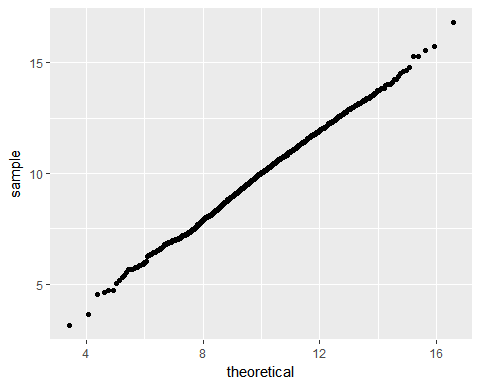
\includegraphics[width=0.6\linewidth]{ProcAnFinDataR_ed_1_files/figure-latex/unnamed-chunk-409-1} \end{center}

In the previous code, we simulate random normal variables with mean 10
and standard deviation equal to 2. As you can see, the QQ plot is close
to a straight line, meaning the empirical distribution of the simulated
data is close to a Normal distribution. Since we used artificial data
from the aforementioned distribution, this result is not surprising!

Now, let's try it for our dataset of stock's returns. We will randomly
select 4 stocks, create a new column, called \texttt{norm.ret}, with the
normalized values of the returns. The normalization procedure works as
follows; we subtract the mean for each return and divide the result by
the standard deviations. This procedure must be executed on an
individual basis for each stock. After that, we compare the resulting
distribution against a standard Normal with mean zero and deviation
equal to 1. The following code does this operation.

\begin{Shaded}
\begin{Highlighting}[]
\CommentTok{# fix seed}
\KeywordTok{set.seed}\NormalTok{(}\DecValTok{45}\NormalTok{)}

\CommentTok{# select 4 stock randomly and filter from my.df}
\NormalTok{my.tickers <-}\StringTok{ }\KeywordTok{sample}\NormalTok{(}\KeywordTok{unique}\NormalTok{(my.df}\OperatorTok{$}\NormalTok{ticker), }\DecValTok{4}\NormalTok{)}
\NormalTok{temp.df <-}\StringTok{ }\KeywordTok{filter}\NormalTok{(my.df, ticker }\OperatorTok\StringTok{ }\NormalTok{my.tickers)}

\CommentTok{# set function for normalization}
\NormalTok{norm.vec <-}\StringTok{ }\ControlFlowTok{function}\NormalTok{(y)\{}
  \CommentTok{# Normalizes a vector by subtracting mean and dividing}
  \CommentTok{# by the standard deviation}
  \CommentTok{#}
  \CommentTok{# Args:}
  \CommentTok{#   y - numerical vector}
  \CommentTok{#}
  \CommentTok{# Returns:}
  \CommentTok{#   A normalized vector}
  
\NormalTok{  y.norm <-}\StringTok{ }\NormalTok{(y}\OperatorTok{-}\KeywordTok{mean}\NormalTok{(y, }\DataTypeTok{na.rm =} \OtherTok{TRUE}\NormalTok{))}\OperatorTok{/}\KeywordTok{sd}\NormalTok{(y, }\DataTypeTok{na.rm =} \OtherTok{TRUE}\NormalTok{)}
  \KeywordTok{return}\NormalTok{(y.norm)}
\NormalTok{\}}

\CommentTok{# apply function  }
\NormalTok{my.l <-}\StringTok{ }\KeywordTok{tapply}\NormalTok{(}\DataTypeTok{X =}\NormalTok{ temp.df}\OperatorTok{$}\NormalTok{ret, }
               \DataTypeTok{INDEX =} \KeywordTok{factor}\NormalTok{(temp.df}\OperatorTok{$}\NormalTok{ticker), }
               \DataTypeTok{FUN =}\NormalTok{ norm.vec)}

\CommentTok{# reorder list (tapply sorts alphabetically)}
\NormalTok{my.l <-}\StringTok{ }\NormalTok{my.l[}\KeywordTok{as.character}\NormalTok{(}\KeywordTok{unique}\NormalTok{(temp.df}\OperatorTok{$}\NormalTok{ticker))]}

\CommentTok{# save new column norm.ret}
\NormalTok{temp.df}\OperatorTok{$}\NormalTok{norm.ret <-}\StringTok{ }\KeywordTok{unlist}\NormalTok{(my.l)}

\CommentTok{# plot it!}
\NormalTok{p <-}\StringTok{ }\KeywordTok{ggplot}\NormalTok{(}\DataTypeTok{data =}\NormalTok{ temp.df, }\KeywordTok{aes}\NormalTok{(}\DataTypeTok{sample =}\NormalTok{ norm.ret)) }
\NormalTok{p <-}\StringTok{ }\NormalTok{p }\OperatorTok{+}\StringTok{ }\KeywordTok{geom_qq}\NormalTok{()}
\NormalTok{p <-}\StringTok{ }\NormalTok{p }\OperatorTok{+}\StringTok{ }\KeywordTok{facet_wrap}\NormalTok{(}\OperatorTok{~}\NormalTok{ticker)}

\KeywordTok{print}\NormalTok{(p)}
\end{Highlighting}
\end{Shaded}

\begin{center}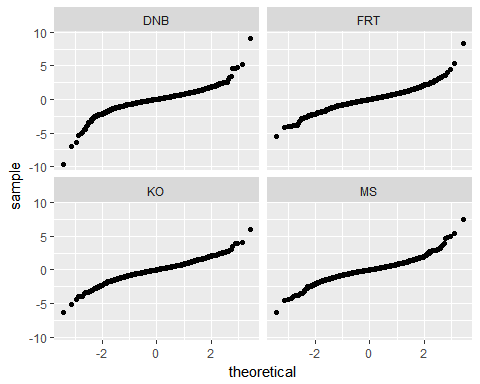
\includegraphics[width=0.6\linewidth]{ProcAnFinDataR_ed_1_files/figure-latex/unnamed-chunk-410-1} \end{center}

As you can see, the result is not visually similar to the result found
for the simulated distribution. In the extreme values of the normalized
returns distributions, we see a higher proportion of cases, when
comparing to the theoretical distribution. Such a result is well-known
and called \emph{fat tails}. This means the Normal distribution does a
bad job describing empirical returns from the stock market. This issue
is particularly important in the calculation of risk estimates, where a
\emph{fat tail} will underestimate the likelihood of an extreme loss.

\section{Saving Graphics to a File}\label{saving-graphics-to-a-file}

To save pictures created with \texttt{ggplot}, use function
\texttt{ggsave}. It takes as input the name of the file, including path
and extension (\emph{.jpg}, \emph{.png}, etc). If the figure object
\texttt{p} is not explicitly set, the last generated graph will be
saved. One suggestion is to give preference to the \emph{png} format,
which is more commonly accepted for publication due to its higher
printing quality. If necessary, you can set the resolution using
argument \texttt{dpi}.

Consider the following example, where we create a graph and save it to a
file, called \texttt{MyPrices.png}, available at folder
\texttt{fig\_ggplot}: \index{ggplot2!ggsave} \index{MyPrices.png}

\begin{Shaded}
\begin{Highlighting}[]
\KeywordTok{library}\NormalTok{(dplyr)}
\CommentTok{# fix seed}
\KeywordTok{set.seed}\NormalTok{(}\DecValTok{40}\NormalTok{)}

\CommentTok{# select 4 stocks randomly}
\NormalTok{my.tickers <-}\StringTok{ }\KeywordTok{sample}\NormalTok{(}\KeywordTok{unique}\NormalTok{(my.df}\OperatorTok{$}\NormalTok{ticker), }\DecValTok{4}\NormalTok{)}

\NormalTok{p <-}\StringTok{ }\NormalTok{my.df }\OperatorTok
\StringTok{  }\KeywordTok{filter}\NormalTok{(ticker }\OperatorTok\StringTok{ }\NormalTok{my.tickers) }\OperatorTok
\StringTok{  }\KeywordTok{ggplot}\NormalTok{(}\KeywordTok{aes}\NormalTok{(}\DataTypeTok{x =}\NormalTok{ ref.date, }\DataTypeTok{y =}\NormalTok{ price.adjusted, }\DataTypeTok{color =}\NormalTok{ ticker)) }\OperatorTok{+}\StringTok{ }
\StringTok{  }\KeywordTok{geom_line}\NormalTok{() }\OperatorTok{+}\StringTok{ }
\StringTok{  }\KeywordTok{labs}\NormalTok{(}\DataTypeTok{x =} \StringTok{'Date'}\NormalTok{, }
       \DataTypeTok{y =} \StringTok{'Adjusted closing prices'}\NormalTok{)}
    
\NormalTok{my.fig.file <-}\StringTok{ 'fig_ggplot/MyPrices.png'}
\KeywordTok{ggsave}\NormalTok{(}\DataTypeTok{filename =}\NormalTok{ my.fig.file, }
       \DataTypeTok{plot=}\NormalTok{p,}
       \DataTypeTok{dpi =} \DecValTok{600}\NormalTok{)}
\end{Highlighting}
\end{Shaded}

You can verify the creation of the file with function
\texttt{list.files}: \index{base!list.files}

\begin{Shaded}
\begin{Highlighting}[]
\KeywordTok{print}\NormalTok{(}\KeywordTok{list.files}\NormalTok{(}\StringTok{'fig_ggplot'}\NormalTok{))}
\end{Highlighting}
\end{Shaded}

\begin{verbatim}
## [1] "MyPrices.png"
\end{verbatim}

As expected, the file is available in folder \texttt{fig\_ggplot}, and
it is ready to be inserted into a technical report or scientific
article.

\hypertarget{programming}{\chapter{Programming and Data Analysis with
R}\label{programming}}

In chapters \ref{BasicObjects}, \ref{DataStructureObjects}, and
\ref{importing}, we learned the ecosystem of objects in R and studied
the procedures for importing datasets from local files and the web.
Here, we will address programming with R and processing data. This
includes the creation of custom functions, structured repetition of code
(\emph{loops}), and conditional execution. A section about one of the
most popular packages in CRAN, \texttt{dplyr}, is also included. The
concepts presented here are valuable. Based on it, you'll be able to
solve several computational problems in your data analysis.

\section{Creating Functions}\label{creating-functions}

As emphasized in an earlier chapter, \textbf{the use of functions is in
the heart of R}. Any procedure can be written to a function. Using
functions organizes code and increases the applicability of generic
procedures. It makes it easy to fix bugs in the code. If you are using a
function in many places of a script, you only need to change it in one
place. For example, consider creating a procedure that cleans a database
by removing outliers and \texttt{NA} cases. This procedure can be
written as a function and be used in different \texttt{dataframes}. If
the author of the function must apply the same procedure in the future,
simply load the previously written function and use it again.

A function can be further developed, so its applicability increases. If
we need to use it in a slightly different way, we can add options using
arguments. By using functions in your work, you'll invest less time in
rewriting repetitive tasks and more in writing new procedures. With time
and experience, a baggage of previously written custom functions will be
available, allowing you to write complex data operations in minutes. In
this section, we will address how to create custom functions in R.
\index{functions}

A function always has three parts: input, processing stage, and output.
The inputs are the information for the solution offered by the function.
Processing is the operation that will produce a result in the function
output. In R, the definition of a function is structured as follows:

\begin{Shaded}
\begin{Highlighting}[]
\NormalTok{my.fct <-}\StringTok{ }\ControlFlowTok{function}\NormalTok{(}\DataTypeTok{arg1 =} \DecValTok{1}\NormalTok{, }\DataTypeTok{arg2 =} \StringTok{'abc'}\NormalTok{, ...)\{}
  \CommentTok{# Description goes here}
  \CommentTok{#}
  \CommentTok{# Args:}
  \CommentTok{#   arg1 - description of arg1 here}
  \CommentTok{#   arg2 - description of arg2 here}
  \CommentTok{#}
  \CommentTok{# Returns:}
  \CommentTok{#   description of returned object goes here}
\NormalTok{  ...}
  
  \KeywordTok{return}\NormalTok{(out)}
  
\NormalTok{\}}
\end{Highlighting}
\end{Shaded}

And, after registering the function in the environment, we can change
its input as necessary, such as in the next example:

\begin{Shaded}
\begin{Highlighting}[]
\NormalTok{out <-}\StringTok{ }\KeywordTok{my.fct}\NormalTok{(}\DataTypeTok{arg1 =} \DecValTok{2}\NormalTok{, }\DataTypeTok{arg2 =} \StringTok{'bcd'}\NormalTok{)}
\end{Highlighting}
\end{Shaded}

The definition of a function is similar to the definition of an object
in R. The main difference is its content is encapsulated by curly braces
(\texttt{\{\ \}}). Objects \emph{arg1} and \emph{arg2} are the inputs of
the function, the information required to perform a procedure.

Using the equality symbol in this setting, as in \texttt{arg1\ =\ 1},
defines the \emph{default} case, determining the default value if the
user does not set any in the call to the written function. Using default
values is useful to define the most likely choice of the inputs of a
function. This facilitates their use by speeding up the calling process
by the user, who does not need to know and enter values for all possible
options.

Every function will return an object with the \texttt{return} command.
This is usually at the end of the function definition. There is no
restriction on the type of object returned: it can be a \texttt{list}, a
\texttt{numeric} array, or an object of any other class. This
flexibility allows the user to return various information. Just organize
it into a \texttt{list}, \texttt{vector}, or \texttt{dataframe}. The
command \texttt{return} defines the end of the function and the return
of the created object. \index{return} \index{base!return}

As for using the function, you'll first need to register it in the
environment by executing its definition like any other code. A simple
way of doing that is to place the cursor in the second curly brace and
press \emph{control + enter}. The arguments of the function can be set
by position or name. So, if you called function \texttt{my.fct} as
\texttt{my.fct(1,2)}, it will recognize its input as \texttt{arg1=1} and
\texttt{arg2=2}. When you use names, the position of arguments is
irrelevant, i.e., the previous function call is equivalent to
\texttt{my.fct(arg2=2,\ arg1=1)}.

Now, let's create a function that does something useful: takes as input
a numeric vector and outputs its mean. From previous chapters we know
that there is already a function called \texttt{mean} that does this
procedure, but we will write a new one as a showcase. Here is the
function definition:

\begin{Shaded}
\begin{Highlighting}[]
\NormalTok{my.fct <-}\StringTok{ }\ControlFlowTok{function}\NormalTok{(}\DataTypeTok{x =} \KeywordTok{c}\NormalTok{(}\DecValTok{1}\NormalTok{,}\DecValTok{1}\NormalTok{,}\DecValTok{1}\NormalTok{,}\DecValTok{1}\NormalTok{))\{}
  \CommentTok{# Calculates the average of input x}
  \CommentTok{#}
  \CommentTok{# Args: }
  \CommentTok{#     x: a numerical vector}
  \CommentTok{#}
  \CommentTok{# Returns:}
  \CommentTok{#   The mean of x}
  
\NormalTok{  out <-}\StringTok{ }\KeywordTok{sum}\NormalTok{(x)}\OperatorTok{/}\KeywordTok{length}\NormalTok{(x)}
  
  \KeywordTok{return}\NormalTok{(out)}
  
\NormalTok{\}}
\end{Highlighting}
\end{Shaded}

Notice how we set a comment section after the first curly brace to
describe the written function, including its arguments and the returned
value. By giving this quick summary, the user can quickly grasp what the
function does and what to expect from it. From the
\href{https://google.github.io/styleguide/Rguide.xml\#functionlanguage}{Google's
R style manual}:

\begin{quote}
``Functions should contain a comments section immediately below the
function definition line. These comments should consist of a
one-sentence description of the function; a list of the function's
arguments, denoted by Args:, with a description of each (including the
data type); and a description of the return value, denoted by Returns:.
The comments should be descriptive enough that a caller can use the
function without reading any of the function's code.''

--- Google's R style manual
\end{quote}

After writing the function down, we need to execute the code to
\emph{register} the procedure in R. Notice, after running the function's
definition, the name of it appears in panel \emph{environment} of
RStudio. In R, a function is an object, just like atomic vectors,
\texttt{lists}, and \texttt{dataframes}. \index{comments in function}

After executing the function definition in the script, let's test it:

\begin{Shaded}
\begin{Highlighting}[]
\CommentTok{# testing function my.fct}
\NormalTok{my.mean <-}\StringTok{ }\KeywordTok{my.fct}\NormalTok{(}\DataTypeTok{x =} \DecValTok{1}\OperatorTok{:}\DecValTok{100}\NormalTok{)}

\CommentTok{# print result}
\KeywordTok{print}\NormalTok{(my.mean)}
\end{Highlighting}
\end{Shaded}

\begin{verbatim}
## [1] 50.5
\end{verbatim}

The result is 50.5, as expected.

If the function \texttt{my.fct} is called without any input, it will use
the \emph{default} value of \texttt{x\ =\ c\ (1,1,1,1)}. Let's try it:

\begin{Shaded}
\begin{Highlighting}[]
\CommentTok{# calling my.fct without input}
\NormalTok{my.mean <-}\StringTok{ }\KeywordTok{my.fct}\NormalTok{()}

\CommentTok{# print result}
\KeywordTok{print}\NormalTok{(my.mean)}
\end{Highlighting}
\end{Shaded}

\begin{verbatim}
## [1] 1
\end{verbatim}

Again, as expected, the returned value is correct.

Although simple, the previous example can be further refined by
introducing tests for the inputs. Notice how \texttt{my.fct} accepts any
input we give. If we defined \texttt{x} as a \texttt{character} object,
the function would still accept it and try to execute the command in
\texttt{out\ \textless{}-\ sum(x)/length(x)}. The problem is the
function \texttt{sum} does not accept a \texttt{character} object and it
would return an error. \textbf{By not testing the types of inputs in the
function, we allow for errors that can lead to problems difficult to
identify}. This is especially true for complex functions with many lines
of code.

Correcting this problem is simple: just use a logical test for the class
of \texttt{x} and throw a custom error with function \texttt{stop} if
the class is not \texttt{numeric} or \texttt{integer}. See next:
\index{base!stop}

\begin{Shaded}
\begin{Highlighting}[]
\NormalTok{my.fct <-}\StringTok{ }\ControlFlowTok{function}\NormalTok{(}\DataTypeTok{x =} \KeywordTok{c}\NormalTok{(}\DecValTok{1}\NormalTok{,}\DecValTok{1}\NormalTok{,}\DecValTok{1}\NormalTok{,}\DecValTok{1}\NormalTok{))\{}
  \CommentTok{# Calculates the average of input x}
  \CommentTok{#}
  \CommentTok{# Args: }
  \CommentTok{#   x - a numerical vector}
  \CommentTok{#}
  \CommentTok{# Returns:}
  \CommentTok{#   The mean of x}
  
  \ControlFlowTok{if}\NormalTok{ (}\OperatorTok{!}\NormalTok{(}\KeywordTok{class}\NormalTok{(x) }\OperatorTok\StringTok{ }\KeywordTok{c}\NormalTok{(}\StringTok{'numeric'}\NormalTok{,}\StringTok{'integer'}\NormalTok{)))\{}
    \KeywordTok{stop}\NormalTok{(}\StringTok{'ERROR: x is not numeric or integer'}\NormalTok{)}
\NormalTok{  \}}
  
\NormalTok{  out <-}\StringTok{ }\KeywordTok{sum}\NormalTok{(x)}\OperatorTok{/}\KeywordTok{length}\NormalTok{(x)}
  
  \KeywordTok{return}\NormalTok{(out)}
\NormalTok{\}}
\end{Highlighting}
\end{Shaded}

In the previous code, we use the \texttt{class} function to test the
input type and \texttt{stop} to issue an error. If we tried to set
\texttt{x} as something different than a \texttt{numeric} or
\texttt{integer} object, the execution stops and an error with the
message \texttt{ERROR:\ x\ is\ not\ numeric\ or\ integer} appears on the
prompt. This message helps the user to understand the reason the
function was not executed and give a hint on how to fix it. See an
example next: \index{base!stop}

\begin{Shaded}
\begin{Highlighting}[]
\CommentTok{# using wrong inputs (ERROR)}
\KeywordTok{my.fct}\NormalTok{(}\DataTypeTok{x =} \KeywordTok{c}\NormalTok{(}\StringTok{'a'}\NormalTok{,}\StringTok{'b'}\NormalTok{))}
\end{Highlighting}
\end{Shaded}

\begin{verbatim}
## Error in my.fct(x = c("a", "b")): ERROR: x is not numeric or integer
\end{verbatim}

Going further in developing our function, notice how it does not deal
with \texttt{NA} values in the input. As explained in previous chapter,
if a numeric vector contains \texttt{NA}, the sum of it will also be a
\texttt{NA} object. Have a look:

\begin{Shaded}
\begin{Highlighting}[]
\CommentTok{# sum with NA}
\KeywordTok{print}\NormalTok{(}\KeywordTok{sum}\NormalTok{(}\KeywordTok{c}\NormalTok{(}\DecValTok{1}\NormalTok{, }\DecValTok{2}\NormalTok{, }\DecValTok{3}\NormalTok{, }\OtherTok{NA}\NormalTok{, }\DecValTok{4}\NormalTok{)))}
\end{Highlighting}
\end{Shaded}

\begin{verbatim}
## [1] NA
\end{verbatim}

The problem with the \texttt{NA} is this object is contagious and will
turn everything it touches into a \texttt{NA}! It is possible that, in
using function \texttt{my.fct}, the user will introduce a bug in his
code that is difficult to identify.

To handle \texttt{NA} values in function \texttt{my.fct}, a possible
solution is to issue a warning message informing the user that input
\texttt{x} contains an \texttt{NA}, remove the \texttt{NA} values from
the input, and proceed with the calculation. The new definition of
\texttt{my.fct} will look like:

\begin{Shaded}
\begin{Highlighting}[]
\NormalTok{my.fct <-}\StringTok{ }\ControlFlowTok{function}\NormalTok{(}\DataTypeTok{x =} \KeywordTok{c}\NormalTok{(}\DecValTok{1}\NormalTok{,}\DecValTok{1}\NormalTok{,}\DecValTok{1}\NormalTok{,}\DecValTok{1}\NormalTok{))\{}
  \CommentTok{# Calculates the average of input x}
  \CommentTok{#}
  \CommentTok{# Args: }
  \CommentTok{#   x: a numerical vector}
  \CommentTok{#}
  \CommentTok{# Returns:}
  \CommentTok{#   The mean of x}
  
  \ControlFlowTok{if}\NormalTok{ (}\OperatorTok{!}\NormalTok{(}\KeywordTok{class}\NormalTok{(x) }\OperatorTok\StringTok{ }\KeywordTok{c}\NormalTok{(}\StringTok{'numeric'}\NormalTok{,}\StringTok{'integer'}\NormalTok{)))\{}
    \KeywordTok{stop}\NormalTok{(}\StringTok{'ERROR: x is not numeric or integer'}\NormalTok{)}
\NormalTok{  \}}
  
  \ControlFlowTok{if}\NormalTok{ (}\KeywordTok{any}\NormalTok{(}\KeywordTok{is.na}\NormalTok{(x)))\{}
    \KeywordTok{warning}\NormalTok{(}\StringTok{'Warning: Found NA in x. Removing it.'}\NormalTok{)}
\NormalTok{    x <-}\StringTok{ }\KeywordTok{na.omit}\NormalTok{(x)}
\NormalTok{  \} }
  
\NormalTok{  out <-}\StringTok{ }\KeywordTok{sum}\NormalTok{(x)}\OperatorTok{/}\KeywordTok{length}\NormalTok{(x)}
  
  \KeywordTok{return}\NormalTok{(out)}
\NormalTok{\}}
\end{Highlighting}
\end{Shaded}

For the previous code, we used function \texttt{warning} to issue a
message in the prompt, command \texttt{any(is.na(x))} to test if any
element of \texttt{x} has a \texttt{NA} value, and \texttt{na.omit} to
remove it from the atomic vector. Let's test it: \index{base!warning}
\index{base!is.na} \index{base!na.omit}

\begin{Shaded}
\begin{Highlighting}[]
\CommentTok{# set vector with NA}
\NormalTok{y <-}\StringTok{ }\KeywordTok{c}\NormalTok{(}\DecValTok{1}\NormalTok{,}\DecValTok{2}\NormalTok{,}\DecValTok{3}\NormalTok{, }\OtherTok{NA}\NormalTok{,}\DecValTok{1}\NormalTok{)}

\CommentTok{# test function}
\KeywordTok{print}\NormalTok{(}\KeywordTok{my.fct}\NormalTok{(y))}
\end{Highlighting}
\end{Shaded}

\begin{verbatim}
## Warning in my.fct(y): Warning: Found NA in x. Removing it.
\end{verbatim}

\begin{verbatim}
## [1] 1.75
\end{verbatim}

As we can see, the function acknowledged the existence of a \texttt{NA}
value, issued a warning message, and calculated the mean of \texttt{x}
without the \texttt{NA}.

Using comments and input testing is a good policy in R programming.
\textbf{Writing good R functions takes a lot of work and demands a great
deal of knowledge about R and the underlying operation}. The great thing
about it is you only need to do it once! The function can be used over
and over in different scenarios. With time, you'll build a set of
functions that will help you do your work, and this collection of code
will be your greatest asset. If you have written something that might
interest other people, package the code and send it to CRAN. The
community will appreciate it.

Now, lets move to a more complete example of using functions. As
emphasized in chapter \ref{Financial-data}, a very common task in
financial research is to calculate the returns of one or more stocks.
Notice the calculation of returns must be done for each stock, and we
always lose the first observation. We will have a \texttt{dataframe} in
the long format with prices for several stocks. Based on these prices,
we want to calculate a vector of returns and add it as a new column.

Let's create a function that takes as input a \texttt{dataframe} in the
long format and adds a new \texttt{ret} column to it. For that, we need
to know only the names of the column where prices are stored and the
name of the column with the ticker symbols. Once the returns are
calculated for each stock, we consolidate a full vector using functions
\texttt{tapply} and \texttt{unlist}. So far, we haven't discussed the
use of \texttt{tapply}. For now, it is only necessary to understand it
performs a function for different groups. We'll provide more detail
about \texttt{tapply} in the following section. \index{base!unlist}

First, let's register a function for calculating returns from a vector
of prices.

\begin{Shaded}
\begin{Highlighting}[]
\NormalTok{calc.ret <-}\StringTok{ }\ControlFlowTok{function}\NormalTok{(P) \{}
  \CommentTok{# calculates arithmetic returns from a vector of prices}
  \CommentTok{#}
  \CommentTok{# Args:}
  \CommentTok{#   P - vector of prices (numeric)}
  \CommentTok{#}
  \CommentTok{# Returns:}
  \CommentTok{#   A vector of returns}
  
  \CommentTok{# ret = p_\{t\}/p_\{t-1\} - 1 }
\NormalTok{  my.length <-}\StringTok{ }\KeywordTok{length}\NormalTok{(P)}
\NormalTok{  ret <-}\StringTok{ }\KeywordTok{c}\NormalTok{(}\OtherTok{NA}\NormalTok{, P[}\DecValTok{2}\OperatorTok{:}\NormalTok{my.length]}\OperatorTok{/}\NormalTok{P[}\DecValTok{1}\OperatorTok{:}\NormalTok{(my.length }\OperatorTok{-}\StringTok{ }\DecValTok{1}\NormalTok{)] }\OperatorTok{-}\StringTok{ }\DecValTok{1}\NormalTok{)}
  \KeywordTok{return}\NormalTok{(ret)}
\NormalTok{\}}
\end{Highlighting}
\end{Shaded}

Notice how we kept it simple. Since we will use \texttt{calc.ret} inside
another function, we can leave the error checking process to the main
function. This can take care of \texttt{NA} values or wrong input class.
In the function definition, we set a \texttt{NA} value in the first
element of the return series. We do that because it is important the
return object has the same length as the input, and we always lose the
first observation when calculating returns. So, we need to replace it
with something. We could have simply set a 0 value or the mean of the
returns, but a \texttt{NA} value seems more appropriate.

Now, let's write a function that, using a \texttt{dataframe} as input,
adds a new column with the arithmetic returns based on the column of
prices and tickers. The definition is given next.

\begin{Shaded}
\begin{Highlighting}[]
\NormalTok{df.calc.ret <-}\StringTok{ }\ControlFlowTok{function}\NormalTok{(df.in, colname.price, colname.tickers)\{}
  \CommentTok{# Calculates an arithmetic return series and adds it to input}
  \CommentTok{#}
  \CommentTok{# Args:}
  \CommentTok{#   df.in - a dataframe with columns for prices and tickers}
  \CommentTok{#   colname.price -  the name of the column in input df.in with prices}
  \CommentTok{#   colname.tickers - the name of the column with tickers}
  \CommentTok{#}
  \CommentTok{# Returns:}
  \CommentTok{#     A copy of the input dataframe, but with a new column ret}
  
  \CommentTok{# error checking (classes)}
  \ControlFlowTok{if}\NormalTok{ ( }\OperatorTok{!}\NormalTok{(}\StringTok{'data.frame'} \OperatorTok\StringTok{ }\KeywordTok{class}\NormalTok{(df.in)) ) \{}
    \KeywordTok{stop}\NormalTok{(}\StringTok{'ERROR: df.in should be a data.frame!'}\NormalTok{)}
\NormalTok{  \}}
  
  \ControlFlowTok{if}\NormalTok{ ( }\KeywordTok{class}\NormalTok{(colname.price) }\OperatorTok{!=}\StringTok{ 'character'}\NormalTok{) \{}
    \KeywordTok{stop}\NormalTok{(}\StringTok{'ERROR: colname.price should be a character object!'}\NormalTok{)}
\NormalTok{  \}}
  
  \ControlFlowTok{if}\NormalTok{ ( }\KeywordTok{class}\NormalTok{(colname.tickers) }\OperatorTok{!=}\StringTok{ 'character'}\NormalTok{) \{}
    \KeywordTok{stop}\NormalTok{(}\StringTok{'ERROR: colname.tickers should be a character object!'}\NormalTok{)}
\NormalTok{  \}}
  
  \CommentTok{# error checking (col.names)}
\NormalTok{  my.colnames <-}\StringTok{ }\KeywordTok{colnames}\NormalTok{(df.in)}
  
  \ControlFlowTok{if}\NormalTok{ (}\KeywordTok{any}\NormalTok{(}\OperatorTok{!}\KeywordTok{c}\NormalTok{(colname.price, colname.tickers) }\OperatorTok\StringTok{ }\NormalTok{my.colnames)) \{}
    \KeywordTok{stop}\NormalTok{(}\StringTok{'ERROR: column names dont match with names in df.in!'}\NormalTok{)}
\NormalTok{  \}}
  
  \CommentTok{# error checking (size of df)}
  \ControlFlowTok{if}\NormalTok{ ( }\KeywordTok{nrow}\NormalTok{(df.in) }\OperatorTok{<}\StringTok{ }\DecValTok{2}\NormalTok{) \{}
    \KeywordTok{stop}\NormalTok{(}\StringTok{'ERROR: input df should have at least 2 rows!'}\NormalTok{)}
\NormalTok{  \}}
  
  \CommentTok{# do calc with tapply}
\NormalTok{  my.l <-}\StringTok{ }\KeywordTok{tapply}\NormalTok{(}\DataTypeTok{X =}\NormalTok{ df.in[[colname.price]], }
                 \DataTypeTok{INDEX =}\NormalTok{ df.in[[colname.tickers]], }
                 \DataTypeTok{FUN =}\NormalTok{ calc.ret)}
  
  
  \CommentTok{# restore order of tickers in df.in}
\NormalTok{  my.l <-}\StringTok{ }\NormalTok{my.l[}\KeywordTok{unique}\NormalTok{(df.in[[colname.tickers]])]}
  
  \CommentTok{# set new col in df.in}
\NormalTok{  df.in}\OperatorTok{$}\NormalTok{ret <-}\StringTok{ }\KeywordTok{unlist}\NormalTok{(my.l)}
  
  \CommentTok{# return df}
  \KeywordTok{return}\NormalTok{(df.in)}
\NormalTok{\}}
\end{Highlighting}
\end{Shaded}

That's a lengthy code! But remember, you only need to do it one time.
The function has many error checking procedures that ensure the inputs
are correctly specified. Even though you spend time writing it, you can
reuse it whenever you need it.

Now, let's use the function with the data available in
\texttt{SP500-Stocks\_long.csv}.

\begin{Shaded}
\begin{Highlighting}[]
\KeywordTok{library}\NormalTok{(readr)}

\NormalTok{my.f <-}\StringTok{ 'data/SP500-Stocks_long.csv'}

\CommentTok{# set columns types}
\NormalTok{my.cols <-}\StringTok{ }\KeywordTok{cols}\NormalTok{(}
  \DataTypeTok{price.adjusted =} \KeywordTok{col_double}\NormalTok{(),}
  \DataTypeTok{ref.date =} \KeywordTok{col_date}\NormalTok{(}\DataTypeTok{format =} \StringTok{""}\NormalTok{),}
  \DataTypeTok{ticker =} \KeywordTok{col_character}\NormalTok{()}
\NormalTok{)}

\CommentTok{# import data}
\NormalTok{my.df <-}\StringTok{ }\KeywordTok{read_csv}\NormalTok{(my.f, }\DataTypeTok{col_types =}\NormalTok{ my.cols)}

\CommentTok{# calculate return column}
\NormalTok{my.df <-}\StringTok{ }\KeywordTok{df.calc.ret}\NormalTok{(my.df, }
                     \DataTypeTok{colname.price =} \StringTok{'price.adjusted'}\NormalTok{, }
                     \DataTypeTok{colname.tickers =} \StringTok{'ticker'}\NormalTok{)}
\end{Highlighting}
\end{Shaded}

Let's look at the result:

\begin{Shaded}
\begin{Highlighting}[]
\KeywordTok{print}\NormalTok{(}\KeywordTok{head}\NormalTok{(my.df))}
\end{Highlighting}
\end{Shaded}

\begin{verbatim}
## # A tibble: 6 × 4
##   price.adjusted   ref.date ticker          ret
##            <dbl>     <date>  <chr>        <dbl>
## 1       69.15826 2010-01-04    MMM           NA
## 2       68.72509 2010-01-05    MMM -0.006263503
## 3       69.69973 2010-01-06    MMM  0.014181794
## 4       69.74972 2010-01-07    MMM  0.000717162
## 5       70.24120 2010-01-08    MMM  0.007046423
## 6       69.95798 2010-01-11    MMM -0.004032220
\end{verbatim}

It looks great! The return vector is available in column \texttt{ret}.
Going further, let's remove all \texttt{NA} rows with function
\texttt{complete.cases}, so we only keep the rows with actual values in
all columns. \index{base!complete.cases}

\begin{Shaded}
\begin{Highlighting}[]
\NormalTok{idx <-}\StringTok{ }\KeywordTok{complete.cases}\NormalTok{(my.df)}
\NormalTok{my.df <-}\StringTok{ }\NormalTok{my.df[idx, ]}
\end{Highlighting}
\end{Shaded}

For last, we save the resulting dataset as a \emph{.RData} file. We will
use the data in this \texttt{dataframe} in the following chapters.

\begin{Shaded}
\begin{Highlighting}[]
\KeywordTok{save}\NormalTok{(}\DataTypeTok{list =} \StringTok{'my.df'}\NormalTok{, }
     \DataTypeTok{file =} \StringTok{'data/SP500-Stocks-WithRet.RData'}\NormalTok{)}
\end{Highlighting}
\end{Shaded}

\section{\texorpdfstring{Using Loops
(\texttt{for})}{Using Loops (for)}}\label{using-loops-for}

\emph{Loops} are the most basic command in any programming language.
Briefly, loops allow a structured repetition of code. Consider a
scenario where we have a database composed of 1,000 \emph{.csv} files in
the same folder. Here, we can create a \emph{loop} to load the data
individually, process the resulting \texttt{dataframe} of each file, and
finally, aggregate all imported \texttt{dataframes} into a single object
of the same class. \index{loops}

The great thing about \emph{loops} is the length of it is dynamically
set. Using the previous example, if we had 5,000 files, the loop would
process all 5,000 files. If we had just 500, the \emph{loop} would run
500 times. That means we can encapsulate a generic procedure for
processing all found files in a particular folder. With it, you have at
your reach a tool for the execution of any sequential process.

The structure of a \emph{loop} in R follows:

\begin{Shaded}
\begin{Highlighting}[]
\ControlFlowTok{for}\NormalTok{ (i }\ControlFlowTok{in}\NormalTok{ i.vec)\{}
\NormalTok{  ...}
\NormalTok{\}}
\end{Highlighting}
\end{Shaded}

In the previous code, command \texttt{for} indicates the beginning of a
\emph{loop}. Object \texttt{i} in \texttt{(i\ in\ i.vec)} is the
iterator of the \emph{loop}. This iterator will change its value in each
iteration, taking each individual value contained in \texttt{i.vec}.
Note the \emph{loop} is encapsulated by curly braces (\texttt{\{\}}).
These are important, as they define where the \emph{loop} starts and
where it ends. The indentation (use of bigger margins) is also important
for visual cues, but not necessary. Consider the following practical
example:

\begin{Shaded}
\begin{Highlighting}[]
\CommentTok{# set seq}
\NormalTok{my.seq <-}\StringTok{ }\KeywordTok{seq}\NormalTok{(}\OperatorTok{-}\DecValTok{5}\NormalTok{,}\DecValTok{5}\NormalTok{)}

\CommentTok{# do loop}
\ControlFlowTok{for}\NormalTok{ (i }\ControlFlowTok{in}\NormalTok{ my.seq)\{}
  \KeywordTok{cat}\NormalTok{(}\KeywordTok{paste}\NormalTok{(}\StringTok{'}\CharTok{\textbackslash{}n}\StringTok{The value of i is'}\NormalTok{,i))}
\NormalTok{\}}
\end{Highlighting}
\end{Shaded}

\begin{verbatim}
## 
## The value of i is -5
## The value of i is -4
## The value of i is -3
## The value of i is -2
## The value of i is -1
## The value of i is 0
## The value of i is 1
## The value of i is 2
## The value of i is 3
## The value of i is 4
## The value of i is 5
\end{verbatim}

In the code, we created a sequence from -5 to 5 and presented a text for
each element with the \texttt{cat} function. Notice how we also broke
the prompt line with
\texttt{\textquotesingle{}\textbackslash{}n\textquotesingle{}}. The
\emph{loop} starts with \texttt{i=-5}, execute command
\texttt{cat(paste(\textquotesingle{}\textbackslash{}nThe\ value\ of\ i\ is\textquotesingle{},\ -5))},
proceed to the next iteration by setting \texttt{i=-4}, rerun the
\texttt{cat} command, and so on. At its final iteration, the value of
\texttt{i} is \texttt{5}.

The iterated sequence in the \emph{loop} is not exclusive to numerical
vectors. Any type of vector or list may be used. See next:

\begin{Shaded}
\begin{Highlighting}[]
\CommentTok{# set char vec}
\NormalTok{my.char.vec <-}\StringTok{ }\NormalTok{letters[}\DecValTok{1}\OperatorTok{:}\DecValTok{5}\NormalTok{]}

\CommentTok{# loop it!}
\ControlFlowTok{for}\NormalTok{ (i.char }\ControlFlowTok{in}\NormalTok{ my.char.vec)\{}
  \KeywordTok{cat}\NormalTok{(}\KeywordTok{paste}\NormalTok{(}\StringTok{'}\CharTok{\textbackslash{}n}\StringTok{The value of i.char is'}\NormalTok{, i.char))}
\NormalTok{\}}
\end{Highlighting}
\end{Shaded}

\begin{verbatim}
## 
## The value of i.char is a
## The value of i.char is b
## The value of i.char is c
## The value of i.char is d
## The value of i.char is e
\end{verbatim}

The same goes for \texttt{lists}:

\begin{Shaded}
\begin{Highlighting}[]
\CommentTok{# set list}
\NormalTok{my.l <-}\StringTok{ }\KeywordTok{list}\NormalTok{(}\DataTypeTok{x =} \DecValTok{1}\OperatorTok{:}\DecValTok{5}\NormalTok{, }
             \DataTypeTok{y =} \KeywordTok{c}\NormalTok{(}\StringTok{'abc'}\NormalTok{,}\StringTok{'dfg'}\NormalTok{), }
             \DataTypeTok{z =} \KeywordTok{factor}\NormalTok{(}\StringTok{'A'}\NormalTok{,}\StringTok{'B'}\NormalTok{,}\StringTok{'C'}\NormalTok{,}\StringTok{'D'}\NormalTok{))}

\CommentTok{# loop list}
\ControlFlowTok{for}\NormalTok{ (i.l }\ControlFlowTok{in}\NormalTok{ my.l)\{}
  
  \KeywordTok{cat}\NormalTok{(}\KeywordTok{paste0}\NormalTok{(}\StringTok{'}\CharTok{\textbackslash{}n}\StringTok{The class of i.l is '}\NormalTok{, }\KeywordTok{class}\NormalTok{(i.l), }\StringTok{'. '}\NormalTok{))}
  \KeywordTok{cat}\NormalTok{(}\KeywordTok{paste0}\NormalTok{(}\StringTok{'The number of elements is '}\NormalTok{, }\KeywordTok{length}\NormalTok{(i.l), }\StringTok{'.'}\NormalTok{))}
  
\NormalTok{\}}
\end{Highlighting}
\end{Shaded}

\begin{verbatim}
## 
## The class of i.l is integer. The number of elements is 5.
## The class of i.l is character. The number of elements is 2.
## The class of i.l is factor. The number of elements is 1.
\end{verbatim}

In the definition of \emph{loops}, the iterator does not have to be the
only object incremented in each iteration. We can create other objects
and increment them using a simple sum operation. See next:

\begin{Shaded}
\begin{Highlighting}[]
\CommentTok{# set vec and iterators}
\NormalTok{my.vec <-}\StringTok{ }\KeywordTok{seq}\NormalTok{(}\DecValTok{1}\OperatorTok{:}\DecValTok{5}\NormalTok{)}
\NormalTok{my.x <-}\StringTok{ }\DecValTok{5}
\NormalTok{my.z <-}\StringTok{ }\DecValTok{10}

\ControlFlowTok{for}\NormalTok{ (i }\ControlFlowTok{in}\NormalTok{ my.vec)\{}
  \CommentTok{# iterate "manually"}
\NormalTok{  my.x <-}\StringTok{ }\NormalTok{my.x }\OperatorTok{+}\StringTok{ }\DecValTok{1}
\NormalTok{  my.z <-}\StringTok{ }\NormalTok{my.z }\OperatorTok{+}\StringTok{ }\DecValTok{2}
  
  \KeywordTok{cat}\NormalTok{(}\StringTok{'}\CharTok{\textbackslash{}n}\StringTok{Value of i = '}\NormalTok{, i, }
      \StringTok{' | Value of my.x = '}\NormalTok{, my.x, }
      \StringTok{' | Value of my.z = '}\NormalTok{, my.z)}
\NormalTok{\}}
\end{Highlighting}
\end{Shaded}

\begin{verbatim}
## 
## Value of i =  1  | Value of my.x =  6  | Value of my.z =  12
## Value of i =  2  | Value of my.x =  7  | Value of my.z =  14
## Value of i =  3  | Value of my.x =  8  | Value of my.z =  16
## Value of i =  4  | Value of my.x =  9  | Value of my.z =  18
## Value of i =  5  | Value of my.x =  10  | Value of my.z =  20
\end{verbatim}

Using nested \emph{loops}, that is, a \emph{loop} inside of another
\emph{loop} is also possible. See the following example, where we
present all the elements of a matrix:

\begin{Shaded}
\begin{Highlighting}[]
\CommentTok{# set matrix}
\NormalTok{my.mat <-}\StringTok{ }\KeywordTok{matrix}\NormalTok{(}\DecValTok{1}\OperatorTok{:}\DecValTok{9}\NormalTok{, }\DataTypeTok{nrow =} \DecValTok{3}\NormalTok{)}

\CommentTok{# loop all values of matrix}
\ControlFlowTok{for}\NormalTok{ (i }\ControlFlowTok{in} \KeywordTok{seq}\NormalTok{(}\DecValTok{1}\NormalTok{,}\KeywordTok{nrow}\NormalTok{(my.mat)))\{}
  \ControlFlowTok{for}\NormalTok{ (j }\ControlFlowTok{in} \KeywordTok{seq}\NormalTok{(}\DecValTok{1}\NormalTok{,}\KeywordTok{ncol}\NormalTok{(my.mat)))\{}
    \KeywordTok{cat}\NormalTok{(}\KeywordTok{paste0}\NormalTok{(}\StringTok{'}\CharTok{\textbackslash{}n}\StringTok{Element ['}\NormalTok{, i, }\StringTok{', '}\NormalTok{, j, }\StringTok{'] = '}\NormalTok{, my.mat[i,j]))}
\NormalTok{  \}}
\NormalTok{\}}
\end{Highlighting}
\end{Shaded}

\begin{verbatim}
## 
## Element [1, 1] = 1
## Element [1, 2] = 4
## Element [1, 3] = 7
## Element [2, 1] = 2
## Element [2, 2] = 5
## Element [2, 3] = 8
## Element [3, 1] = 3
## Element [3, 2] = 6
## Element [3, 3] = 9
\end{verbatim}

Let's do a more complex example using data files. We will create several
files with random data in our computer and save them in a folder named
\texttt{many\_datafiles}. This is accomplished with the following
script:

\begin{Shaded}
\begin{Highlighting}[]
\CommentTok{# set number of files to create}
\NormalTok{n.files <-}\StringTok{ }\DecValTok{10}

\CommentTok{# set first part of saved files}
\NormalTok{pattern.name <-}\StringTok{ 'myfiles_'}

\CommentTok{# set dir}
\NormalTok{out.dir <-}\StringTok{ 'many_datafiles/'}

\CommentTok{# test if out.dir exists, if not, create it}
\ControlFlowTok{if}\NormalTok{ (}\OperatorTok{!}\KeywordTok{dir.exists}\NormalTok{(out.dir))\{}
  \KeywordTok{dir.create}\NormalTok{(out.dir)   }
\NormalTok{\} }

\CommentTok{# clean up folder before creating new files}
\KeywordTok{file.remove}\NormalTok{(}\KeywordTok{list.files}\NormalTok{(out.dir, }\DataTypeTok{full.names =} \OtherTok{TRUE}\NormalTok{)) }
\end{Highlighting}
\end{Shaded}

\begin{verbatim}
## logical(0)
\end{verbatim}

\begin{Shaded}
\begin{Highlighting}[]
\CommentTok{# set vec with filenames}
\NormalTok{file.names <-}\StringTok{ }\KeywordTok{paste0}\NormalTok{(out.dir, pattern.name, }\KeywordTok{seq}\NormalTok{(}\DecValTok{1}\NormalTok{,n.files), }\StringTok{'.csv'}\NormalTok{)}

\CommentTok{# loop it!}
\ControlFlowTok{for}\NormalTok{ (i.file }\ControlFlowTok{in}\NormalTok{ file.names)\{}
  \CommentTok{# create temp df}
\NormalTok{  temp.df <-}\StringTok{ }\KeywordTok{data.frame}\NormalTok{(}\DataTypeTok{x =} \KeywordTok{runif}\NormalTok{(}\DecValTok{100}\NormalTok{))}
  
  \CommentTok{# write it!}
  \KeywordTok{write.csv}\NormalTok{(}\DataTypeTok{x =}\NormalTok{ temp.df, }\DataTypeTok{file =}\NormalTok{ i.file)}
\NormalTok{\}}
\end{Highlighting}
\end{Shaded}

In the previous example, we used function \texttt{if} in
\texttt{if\ (!dir.exists(out.dir))} to test if folder
\texttt{many\_datafiles} existed. If it did not, we create it in the
current working directory. Before running the loop, we remove all files
in \texttt{out.dir} with command
\texttt{file.remove(list.files(out.dir,\ full.names\ =\ TRUE))}.

In the \emph{loop}, we used function \texttt{runif} to create 100 random
numbers between \emph{0} and \emph{1}, so each \emph{dataframe} created
in \texttt{temp.df} differs from the other. Notice how the \emph{loop}
size is set by object \texttt{n.files}. If we wanted to create
\emph{10,000} files, all we need to do is set \texttt{n.files\ =\ 10000}
and the rest of the code will adjust accordingly. It becomes clear that
\emph{loops} are a powerful and flexible procedure that can be used in
many situations.

Now, let's check if the files are in the folder:

\begin{Shaded}
\begin{Highlighting}[]
\CommentTok{# check files}
\KeywordTok{print}\NormalTok{(}\KeywordTok{list.files}\NormalTok{(out.dir))}
\end{Highlighting}
\end{Shaded}

\begin{verbatim}
##  [1] "myfiles_1.csv"  "myfiles_10.csv" "myfiles_2.csv" 
##  [4] "myfiles_3.csv"  "myfiles_4.csv"  "myfiles_5.csv" 
##  [7] "myfiles_6.csv"  "myfiles_7.csv"  "myfiles_8.csv" 
## [10] "myfiles_9.csv"
\end{verbatim}

As expected, the files are there. To complete the example, we will
import the contents of these files and aggregate all information into a
single \texttt{dataframe} by using another \emph{loop} and functions
\texttt{read.csv} and \texttt{rbind}.

\begin{Shaded}
\begin{Highlighting}[]
\CommentTok{# set empty df}
\NormalTok{df.agg <-}\StringTok{ }\KeywordTok{data.frame}\NormalTok{()}
\ControlFlowTok{for}\NormalTok{ (i.file }\ControlFlowTok{in}\NormalTok{ file.names)\{}
  \CommentTok{# read file}
\NormalTok{  temp.df <-}\StringTok{ }\KeywordTok{read.csv}\NormalTok{(i.file)}
  
  \CommentTok{# row bind }
\NormalTok{  df.agg <-}\StringTok{ }\KeywordTok{rbind}\NormalTok{(df.agg, temp.df)}
\NormalTok{\}}

\KeywordTok{print}\NormalTok{(}\KeywordTok{head}\NormalTok{(df.agg))}
\end{Highlighting}
\end{Shaded}

\begin{verbatim}
##   X         x
## 1 1 0.1950091
## 2 2 0.4612009
## 3 3 0.2035352
## 4 4 0.5908492
## 5 5 0.3738881
## 6 6 0.1412981
\end{verbatim}

In the previous code, notice how we bind all \texttt{dataframes} with
\texttt{df.agg\ \textless{}-\ rbind(df.agg,\ temp.df)}. So, the size of
\texttt{df.agg} increases with each iteration of the \emph{loop}. Object
\texttt{df.agg} has 1000 rows and 2 columns. The extra column is the row
names of the \texttt{dataframe}, which is saved by default in the
\emph{.csv} file. Looking at the contents of \texttt{df.agg}, we can see
the code performed as expected, where column \texttt{x} contains
numerical values between \emph{0} and \emph{1}, just as set in the
previous chunk of code. \index{binding dataframes with loop}

Another practical example of using \emph{loops} is processing data
according to groups. If we have a price dataset for several tickers and
we want to calculate the average price of each stock, we can use a
\emph{loop} for that. In this example, we will again use the data from
file \texttt{SP500-Stocks\_long.csv}.

\begin{Shaded}
\begin{Highlighting}[]
\CommentTok{# read data}
\NormalTok{my.f <-}\StringTok{ 'data/SP500-Stocks_long.csv'}
\NormalTok{my.df <-}\StringTok{ }\KeywordTok{read.csv}\NormalTok{(my.f, }\DataTypeTok{colClasses =} \KeywordTok{c}\NormalTok{(}\StringTok{'numeric'}\NormalTok{, }\StringTok{'Date'}\NormalTok{,}\StringTok{'factor'}\NormalTok{))}

\CommentTok{# find unique tickers in column ticker}
\NormalTok{unique.tickers <-}\StringTok{ }\KeywordTok{unique}\NormalTok{(my.df}\OperatorTok{$}\NormalTok{ticker)}

\CommentTok{# create empty df}
\NormalTok{tab.out <-}\StringTok{ }\KeywordTok{data.frame}\NormalTok{()}

\CommentTok{# loop tickers}
\ControlFlowTok{for}\NormalTok{ (i.ticker }\ControlFlowTok{in}\NormalTok{ unique.tickers)\{}
  
  \CommentTok{# create temp df with ticker i.ticker}
\NormalTok{  temp <-}\StringTok{ }\NormalTok{my.df[my.df}\OperatorTok{$}\NormalTok{ticker}\OperatorTok{==}\NormalTok{i.ticker, ]}
  
  \CommentTok{# row bind i.ticker and mean.price}
\NormalTok{  tab.out <-}\StringTok{ }\KeywordTok{rbind}\NormalTok{(tab.out, }
                   \KeywordTok{data.frame}\NormalTok{(}\DataTypeTok{ticker =}\NormalTok{ i.ticker,}
                              \DataTypeTok{mean.price =} \KeywordTok{mean}\NormalTok{(temp}\OperatorTok{$}\NormalTok{price.adjusted)))}
  
\NormalTok{\}}

\CommentTok{# print result}
\KeywordTok{print}\NormalTok{(tab.out[}\DecValTok{1}\OperatorTok{:}\DecValTok{10}\NormalTok{, ])}
\end{Highlighting}
\end{Shaded}

\begin{verbatim}
##    ticker mean.price
## 1     MMM  110.90200
## 2     ABT   32.11558
## 3     ACN   70.60025
## 4    ATVI   19.04112
## 5     AYI  112.67233
## 6    ADBE   55.24791
## 7     AAP  103.19876
## 8     AES   11.19658
## 9     AET   65.73250
## 10    AMG  143.31837
\end{verbatim}

In the code, we used function \texttt{unique} to find out the names of
all the tickers in the dataset. Soon after, we create an empty
\emph{dataframe} to save the results and a loop to filter the data of
each stock sequentially and average its prices. At the end of the
\emph{loop}, we use function \texttt{rbind} to paste the results of each
stock with the results of the main table. As you can see, we can use the
data to perform group calculations with \emph{loop}. There are, however,
better ways of doing this procedure in R using native \texttt{apply}
functions or package \texttt{dplyr}, as we will soon learn.
\index{base!unique}

\section{\texorpdfstring{Conditional Statements (\texttt{if},
\texttt{else},
\texttt{switch})}{Conditional Statements (if, else, switch)}}\label{conditional-statements-if-else-switch}

Making binary decisions of type \emph{yes} or \emph{no} is common
programming practice. If a condition is found true, a specific code is
executed. If it is false, other command lines are executed. These
decisions define the conditional statements. In R, we can write them
using the following structure:

\begin{Shaded}
\begin{Highlighting}[]
\CommentTok{# skeleton for if statement}
\ControlFlowTok{if}\NormalTok{ (cond)\{}
  
\NormalTok{  CodeIfTRUE...}
  
\NormalTok{\} }\ControlFlowTok{else}\NormalTok{ \{}
  
\NormalTok{  CodeIfFALSE...}
  
\NormalTok{\}}
\end{Highlighting}
\end{Shaded}

The place holder \texttt{cond} is the condition to be evaluated, taking
only two values: \texttt{TRUE} or \texttt{FALSE}. The result of the
condition must be a single logical element. With finding a \texttt{TRUE}
value to \texttt{cond}, the code in \texttt{CodeIfTRUE} will run.
Otherwise, where we find a \texttt{FALSE} value in \texttt{cond}, the
code in \texttt{CodeIfFALSE} will be executed. A practical example based
on a \emph{loop} is presented next: \index{base!if}
\index{conditional statements}

\begin{Shaded}
\begin{Highlighting}[]
\CommentTok{# set vec and threshold}
\NormalTok{my.x <-}\StringTok{ }\DecValTok{1}\OperatorTok{:}\DecValTok{10}
\NormalTok{my.thresh <-}\StringTok{ }\DecValTok{5}

\ControlFlowTok{for}\NormalTok{ (i }\ControlFlowTok{in}\NormalTok{ my.x)\{}
  \ControlFlowTok{if}\NormalTok{ (i }\OperatorTok{>}\StringTok{ }\NormalTok{my.thresh)\{}
    \KeywordTok{cat}\NormalTok{(}\StringTok{'}\CharTok{\textbackslash{}n}\StringTok{Value of '}\NormalTok{, i, }\StringTok{' is higher than '}\NormalTok{, my.thresh)}
\NormalTok{  \} }\ControlFlowTok{else}\NormalTok{ \{}
    \KeywordTok{cat}\NormalTok{(}\StringTok{'}\CharTok{\textbackslash{}n}\StringTok{Value of '}\NormalTok{, i, }\StringTok{' is lower or equal than '}\NormalTok{, my.thresh)}
\NormalTok{  \}}
\NormalTok{\}}
\end{Highlighting}
\end{Shaded}

\begin{verbatim}
## 
## Value of  1  is lower or equal than  5
## Value of  2  is lower or equal than  5
## Value of  3  is lower or equal than  5
## Value of  4  is lower or equal than  5
## Value of  5  is lower or equal than  5
## Value of  6  is higher than  5
## Value of  7  is higher than  5
## Value of  8  is higher than  5
## Value of  9  is higher than  5
## Value of  10  is higher than  5
\end{verbatim}

If we want to apply more than one logical condition, we can use command
\texttt{else\ if} and \texttt{else}. See an example next:
\index{base!else}

\begin{Shaded}
\begin{Highlighting}[]
\ControlFlowTok{for}\NormalTok{ (i }\ControlFlowTok{in}\NormalTok{ my.x)\{}
  \ControlFlowTok{if}\NormalTok{ (i }\OperatorTok{>}\StringTok{ }\NormalTok{my.thresh)\{}
    \KeywordTok{cat}\NormalTok{(}\StringTok{'}\CharTok{\textbackslash{}n}\StringTok{Value of '}\NormalTok{, i, }\StringTok{' is higher than '}\NormalTok{, my.thresh)}
\NormalTok{  \} }\ControlFlowTok{else} \ControlFlowTok{if}\NormalTok{ (i}\OperatorTok{==}\NormalTok{my.thresh) \{}
    \KeywordTok{cat}\NormalTok{(}\StringTok{'}\CharTok{\textbackslash{}n}\StringTok{Value of '}\NormalTok{, i, }\StringTok{' is equal to '}\NormalTok{, my.thresh)}
\NormalTok{  \} }\ControlFlowTok{else}\NormalTok{ \{}
    \KeywordTok{cat}\NormalTok{(}\StringTok{'}\CharTok{\textbackslash{}n}\StringTok{Value of '}\NormalTok{, i, }\StringTok{' is lower than '}\NormalTok{, my.thresh)}
\NormalTok{  \}}
\NormalTok{\}}
\end{Highlighting}
\end{Shaded}

\begin{verbatim}
## 
## Value of  1  is lower than  5
## Value of  2  is lower than  5
## Value of  3  is lower than  5
## Value of  4  is lower than  5
## Value of  5  is equal to  5
## Value of  6  is higher than  5
## Value of  7  is higher than  5
## Value of  8  is higher than  5
## Value of  9  is higher than  5
## Value of  10  is higher than  5
\end{verbatim}

Another possibility for using conditional executions is function
\texttt{switch}, designed to give a better structure for a decision
based on more than two choices. Let's say you want a conditional
execution based on five conditions, A, B, C, and D. For each condition,
you want the code to show a different message. Using \texttt{if}
function, you could do that using this chunk of code:

\begin{Shaded}
\begin{Highlighting}[]
\CommentTok{# set vec}
\NormalTok{my.vec <-}\StringTok{ }\KeywordTok{c}\NormalTok{(}\StringTok{'A'}\NormalTok{, }\StringTok{'D'}\NormalTok{, }\StringTok{'B'}\NormalTok{, }\StringTok{'A'}\NormalTok{, }\StringTok{'C'}\NormalTok{, }\StringTok{'B'}\NormalTok{)}

\ControlFlowTok{for}\NormalTok{ (i.vec }\ControlFlowTok{in}\NormalTok{ my.vec)\{}
  \ControlFlowTok{if}\NormalTok{ (i.vec }\OperatorTok{==}\StringTok{ 'A'}\NormalTok{)\{}
    \KeywordTok{cat}\NormalTok{(}\StringTok{'}\CharTok{\textbackslash{}n}\StringTok{Got an A!'}\NormalTok{)}
\NormalTok{  \} }\ControlFlowTok{else} \ControlFlowTok{if}\NormalTok{ (i.vec }\OperatorTok{==}\StringTok{ 'B'}\NormalTok{) \{}
    \KeywordTok{cat}\NormalTok{(}\StringTok{'}\CharTok{\textbackslash{}n}\StringTok{Got a B!'}\NormalTok{)}
\NormalTok{  \} }\ControlFlowTok{else} \ControlFlowTok{if}\NormalTok{ (i.vec }\OperatorTok{==}\StringTok{ 'C'}\NormalTok{) \{}
    \KeywordTok{cat}\NormalTok{(}\StringTok{'}\CharTok{\textbackslash{}n}\StringTok{Got a C!'}\NormalTok{)}
\NormalTok{  \} }\ControlFlowTok{else} \ControlFlowTok{if}\NormalTok{ (i.vec }\OperatorTok{==}\StringTok{ 'D'}\NormalTok{) \{}
    \KeywordTok{cat}\NormalTok{(}\StringTok{'}\CharTok{\textbackslash{}n}\StringTok{Got a D!'}\NormalTok{)   }
\NormalTok{  \}}
\NormalTok{\}}
\end{Highlighting}
\end{Shaded}

\begin{verbatim}
## 
## Got an A!
## Got a D!
## Got a B!
## Got an A!
## Got a C!
## Got a B!
\end{verbatim}

While the previous code would do what we need, using several
\texttt{else\ if} conditions is not visually elegant. A better way of
doing it is using function \texttt{switch}. See next:

\begin{Shaded}
\begin{Highlighting}[]
\CommentTok{# set vec}
\NormalTok{my.vec <-}\StringTok{ }\KeywordTok{c}\NormalTok{(}\StringTok{'A'}\NormalTok{, }\StringTok{'D'}\NormalTok{, }\StringTok{'B'}\NormalTok{, }\StringTok{'A'}\NormalTok{, }\StringTok{'C'}\NormalTok{, }\StringTok{'B'}\NormalTok{)}

\ControlFlowTok{for}\NormalTok{ (i.vec }\ControlFlowTok{in}\NormalTok{ my.vec)\{}
\NormalTok{  msg.out <-}\StringTok{ }\ControlFlowTok{switch}\NormalTok{(i.vec, }
                  \StringTok{'A'}\NormalTok{ =}\StringTok{ '}\CharTok{\textbackslash{}n}\StringTok{Got an A!'}\NormalTok{,}
                  \StringTok{'B'}\NormalTok{ =}\StringTok{ '}\CharTok{\textbackslash{}n}\StringTok{Got a B!'}\NormalTok{,}
                  \StringTok{'C'}\NormalTok{ =}\StringTok{ '}\CharTok{\textbackslash{}n}\StringTok{Got a C!'}\NormalTok{,}
                  \StringTok{'D'}\NormalTok{ =}\StringTok{ '}\CharTok{\textbackslash{}n}\StringTok{Got a D!'}\NormalTok{)}
  
  \KeywordTok{cat}\NormalTok{(msg.out)}
  
\NormalTok{\}}
\end{Highlighting}
\end{Shaded}

\begin{verbatim}
## 
## Got an A!
## Got a D!
## Got a B!
## Got an A!
## Got a C!
## Got a B!
\end{verbatim}

The main benefit of using \texttt{switch} is the code becomes clear and
easier to understand.

\section{\texorpdfstring{Using \texttt{apply}
Functions}{Using apply Functions}}\label{using-apply-functions}

In R, there is an alternative to the usage of \emph{loops}. Sometimes,
you want simple procedures executed in a vector object. Writing a whole
\emph{loop} for that can be more verbose than needed. Functions from the
\textbf{apply family}: \texttt{sapply}, \texttt{lapply},
\texttt{tapply}, \texttt{mapply}, \texttt{apply} and \texttt{by} can be
used for that purpose.

All procedures using \emph{loops} can be restructured using \emph{apply}
functions and vice versa. The difference of processing speed from one to
the other is negligible. The choice between \emph{loops} and
\emph{apply} functions is determined by the complexity of the operation
and personal taste. Sometimes, \emph{loops} are easier to use. The
opposite can be true in other scenarios. In the author's opinion,
\emph{loops} should be used when complex procedures are performed and
using the structure of an \emph{apply} function is not straightforward.
Now, let's discuss each type of \emph{apply} function.

\subsection{\texorpdfstring{Using
\texttt{lapply}}{Using lapply}}\label{using-lapply}

Function \texttt{lapply} takes as input a \texttt{list} and a function
object. It works by passing each element of the input \texttt{list} to
the object function. The output of each call is aggregated and returned
as an object of class \texttt{list}. Notice how the use of
\texttt{lists} in the input and output of \texttt{lapply} provides
flexibility. You can use it for any object, with no restriction on its
output. See the following example, where we calculate the average of a
series of vectors with different sizes: \index{base!lapply}

\begin{Shaded}
\begin{Highlighting}[]
\CommentTok{# set list}
\NormalTok{my.l <-}\StringTok{ }\KeywordTok{list}\NormalTok{(}\DecValTok{1}\OperatorTok{:}\DecValTok{10}\NormalTok{, }\DecValTok{2}\OperatorTok{:}\DecValTok{5}\NormalTok{, }\DecValTok{10}\OperatorTok{:-}\DecValTok{20}\NormalTok{)}

\CommentTok{# use lapply with mean}
\NormalTok{my.mean.vec <-}\StringTok{ }\KeywordTok{lapply}\NormalTok{(}\DataTypeTok{X =}\NormalTok{ my.l, }\DataTypeTok{FUN =}\NormalTok{ mean)}

\CommentTok{# print result}
\KeywordTok{print}\NormalTok{(my.mean.vec)}
\end{Highlighting}
\end{Shaded}

\begin{verbatim}
## [[1]]
## [1] 5.5
## 
## [[2]]
## [1] 3.5
## 
## [[3]]
## [1] -5
\end{verbatim}

The result shows the means of each vector in \texttt{my.l}, as expected.
We could also pass other options to \texttt{mean} with \texttt{lapply}.
See next, where we use \texttt{na.rm=TRUE}.

\begin{Shaded}
\begin{Highlighting}[]
\CommentTok{# set list}
\NormalTok{my.l <-}\StringTok{ }\KeywordTok{list}\NormalTok{(}\KeywordTok{c}\NormalTok{(}\DecValTok{1}\NormalTok{,}\OtherTok{NA}\NormalTok{,}\DecValTok{2}\NormalTok{), }\KeywordTok{c}\NormalTok{(}\DecValTok{2}\OperatorTok{:}\DecValTok{5}\NormalTok{,}\OtherTok{NA}\NormalTok{), }\DecValTok{10}\OperatorTok{:-}\DecValTok{20}\NormalTok{)}

\CommentTok{# use lapply with mean}
\NormalTok{my.mean.vec <-}\StringTok{ }\KeywordTok{lapply}\NormalTok{(}\DataTypeTok{X =}\NormalTok{ my.l, }\DataTypeTok{FUN =}\NormalTok{ mean, }\DataTypeTok{na.rm=}\OtherTok{TRUE}\NormalTok{)}

\CommentTok{# print result}
\KeywordTok{print}\NormalTok{(my.mean.vec)}
\end{Highlighting}
\end{Shaded}

\begin{verbatim}
## [[1]]
## [1] 1.5
## 
## [[2]]
## [1] 3.5
## 
## [[3]]
## [1] -5
\end{verbatim}

Using \texttt{lapply} is useful when utilizing a custom function. Let's
redo the previous example of creating several \emph{.csv} files. The
first step is to create a function that generates these files as we did
with the \emph{loop}.

\begin{Shaded}
\begin{Highlighting}[]
\CommentTok{# function to generate files}
\NormalTok{create.rnd.file <-}\StringTok{ }\ControlFlowTok{function}\NormalTok{(name.file, }\DataTypeTok{N=}\DecValTok{100}\NormalTok{)\{}
  \CommentTok{# Generates a csv file with random content}
  \CommentTok{#}
  \CommentTok{# Args:}
  \CommentTok{#     name.file - name of csv file (character)}
  \CommentTok{# N - number of rows in random dataframe (integer)}
  \CommentTok{#}
  \CommentTok{# Returns:}
  \CommentTok{#     TRUE, if successful}
  
  \ControlFlowTok{if}\NormalTok{ (}\KeywordTok{class}\NormalTok{(name.file)}\OperatorTok{!=}\StringTok{'character'}\NormalTok{)\{}
    \KeywordTok{stop}\NormalTok{(}\StringTok{'ERROR: input name.file is not a character'}\NormalTok{)}
\NormalTok{  \}}
  
  \ControlFlowTok{if}\NormalTok{ ( }\OperatorTok{!}\NormalTok{(}\KeywordTok{class}\NormalTok{(N) }\OperatorTok\StringTok{ }\KeywordTok{c}\NormalTok{(}\StringTok{'numeric'}\NormalTok{,}\StringTok{'integer'}\NormalTok{)) )\{}
    \KeywordTok{stop}\NormalTok{(}\StringTok{'ERROR: input N is not an integer or numeric!'}\NormalTok{)}
\NormalTok{  \}}
  
  \CommentTok{# create random df}
\NormalTok{  temp.df <-}\StringTok{ }\KeywordTok{data.frame}\NormalTok{(}\DataTypeTok{x =} \KeywordTok{runif}\NormalTok{(N))}
  
  \CommentTok{# write it!}
  \KeywordTok{write.csv}\NormalTok{(}\DataTypeTok{x =}\NormalTok{ temp.df, }\DataTypeTok{file =}\NormalTok{ name.file)}
  
  \CommentTok{# return TRUE}
  \KeywordTok{return}\NormalTok{(}\OtherTok{TRUE}\NormalTok{)}
\NormalTok{\}}
\end{Highlighting}
\end{Shaded}

Now, we use function \texttt{create.rnd.file} with \texttt{lapply}:
\index{create.rnd.file}

\begin{Shaded}
\begin{Highlighting}[]
\CommentTok{# set options}
\NormalTok{n.files <-}\StringTok{ }\DecValTok{5}
\NormalTok{pattern.name <-}\StringTok{ 'myfiles_with_lapply_'}
\NormalTok{out.dir <-}\StringTok{ 'many_datafiles/'}

\CommentTok{# set file names}
\NormalTok{file.names <-}\StringTok{ }\KeywordTok{paste0}\NormalTok{(out.dir,pattern.name, }\KeywordTok{seq}\NormalTok{(}\DecValTok{1}\NormalTok{,n.files), }\StringTok{'.csv'}\NormalTok{)}

\CommentTok{# test if out.dir exists, if not, create it}
\ControlFlowTok{if}\NormalTok{ (}\OperatorTok{!}\KeywordTok{dir.exists}\NormalTok{(out.dir))\{}
  \KeywordTok{dir.create}\NormalTok{(out.dir)   }
\NormalTok{\} }

\CommentTok{# clean up folder before creating new files}
\KeywordTok{file.remove}\NormalTok{(}\KeywordTok{list.files}\NormalTok{(out.dir, }\DataTypeTok{full.names =} \OtherTok{TRUE}\NormalTok{)) }
\end{Highlighting}
\end{Shaded}

\begin{verbatim}
##  [1] TRUE TRUE TRUE TRUE TRUE TRUE TRUE TRUE TRUE TRUE
\end{verbatim}

\begin{Shaded}
\begin{Highlighting}[]
\CommentTok{# use lapply}
\NormalTok{out.l <-}\StringTok{ }\KeywordTok{lapply}\NormalTok{(}\DataTypeTok{X =}\NormalTok{ file.names, }\DataTypeTok{FUN =}\NormalTok{ create.rnd.file, }\DataTypeTok{N=}\DecValTok{100}\NormalTok{)}

\CommentTok{# print result}
\KeywordTok{print}\NormalTok{(out.l)}
\end{Highlighting}
\end{Shaded}

\begin{verbatim}
## [[1]]
## [1] TRUE
## 
## [[2]]
## [1] TRUE
## 
## [[3]]
## [1] TRUE
## 
## [[4]]
## [1] TRUE
## 
## [[5]]
## [1] TRUE
\end{verbatim}

Everything worked well in the previous code. The creation of the random
files was a success. Notice the return of \texttt{lapply} is a
\texttt{list}. Whenever you need to apply a function that returns a
complex object, such as the estimation of a model, it is advised to use
\texttt{lapply}.

\subsection{\texorpdfstring{Using
\texttt{sapply}}{Using sapply}}\label{using-sapply}

Function \texttt{sapply} works similarly to \texttt{lapply}. The main
difference is in the type of output. While \texttt{lapply} returns a
list, \texttt{sapply} returns an atomic matrix or vector. See the
following example: \index{base!sapply}

\begin{Shaded}
\begin{Highlighting}[]
\CommentTok{# create list}
\NormalTok{my.l <-}\StringTok{ }\KeywordTok{list}\NormalTok{(}\DecValTok{1}\OperatorTok{:}\DecValTok{10}\NormalTok{, }\DecValTok{2}\OperatorTok{:}\DecValTok{5}\NormalTok{, }\DecValTok{10}\OperatorTok{:-}\DecValTok{20}\NormalTok{)}

\CommentTok{# use sapply}
\NormalTok{my.mean.vec <-}\StringTok{ }\KeywordTok{sapply}\NormalTok{(my.l, mean)}

\CommentTok{# print result}
\KeywordTok{print}\NormalTok{(my.mean.vec)}
\end{Highlighting}
\end{Shaded}

\begin{verbatim}
## [1]  5.5  3.5 -5.0
\end{verbatim}

Using \texttt{sapply} is recommended when the output of the underlying
function is an atomic vector. In such cases, it is unnecessary to return
a flexible object, such as a \texttt{list}.

An important aspect of using \texttt{sapply} is the underlying function
can return more than one value. The result comes from the aggregation of
the individual vectors into a \texttt{matrix}. See the following
example, where we create a function that returns the mean and standard
deviation of a numeric vector:

\begin{Shaded}
\begin{Highlighting}[]
\CommentTok{# set list}
\NormalTok{my.l <-}\StringTok{ }\KeywordTok{list}\NormalTok{(}\KeywordTok{runif}\NormalTok{(}\DecValTok{10}\NormalTok{), }\KeywordTok{runif}\NormalTok{(}\DecValTok{15}\NormalTok{), }\KeywordTok{rnorm}\NormalTok{(}\DecValTok{1000}\NormalTok{))}

\NormalTok{my.fct <-}\StringTok{ }\ControlFlowTok{function}\NormalTok{(x)\{}
  \CommentTok{# Returns mean and standard deviation of a vector}
  \CommentTok{#}
  \CommentTok{# Args: }
  \CommentTok{#   x - numerical vector}
  \CommentTok{#}
  \CommentTok{# Returns:}
  \CommentTok{#   Vector as c(mean(x), sd(x))}
  
  \ControlFlowTok{if}\NormalTok{ (}\OperatorTok{!}\NormalTok{(}\KeywordTok{class}\NormalTok{(x) }\OperatorTok\StringTok{ }\KeywordTok{c}\NormalTok{(}\StringTok{'numeric'}\NormalTok{,}\StringTok{'integer'}\NormalTok{)))\{}
    \KeywordTok{stop}\NormalTok{(}\StringTok{'ERROR: Class of x is not numeric or integer.'}\NormalTok{)}
\NormalTok{  \}}
  
\NormalTok{  x <-}\StringTok{ }\KeywordTok{na.omit}\NormalTok{(x)}
  
\NormalTok{  out <-}\StringTok{ }\KeywordTok{c}\NormalTok{(}\KeywordTok{mean}\NormalTok{(x), }\KeywordTok{sd}\NormalTok{(x))}
  \KeywordTok{return}\NormalTok{(out)}
  
\NormalTok{\}}

\CommentTok{# use sapply}
\NormalTok{my.vec <-}\StringTok{ }\KeywordTok{sapply}\NormalTok{(my.l, my.fct)}

\CommentTok{# check result}
\KeywordTok{print}\NormalTok{(my.vec)}
\end{Highlighting}
\end{Shaded}

\begin{verbatim}
##           [,1]      [,2]       [,3]
## [1,] 0.4102478 0.4090657 0.01050914
## [2,] 0.2842762 0.3344650 0.98690967
\end{verbatim}

When there is more than one output in the underlying function, each row
in the returned object represents a different output of the function
used with \texttt{sapply}, in this case, the mean and standard deviation
of \texttt{x}. The columns indicate the different processed items in
\texttt{my.l}.

A practical use of function \texttt{sapply} in data analysis is the
creation of descriptive tables. Let's use the SP500 data and create a
descriptive analysis of the prices of the different stocks. First, let's
write the function.

\begin{Shaded}
\begin{Highlighting}[]
\NormalTok{describe.vec <-}\StringTok{ }\ControlFlowTok{function}\NormalTok{(x)\{}
  \CommentTok{# Describe numerical vector with mean and other stats}
  \CommentTok{#}
  \CommentTok{# Args:}
  \CommentTok{#   x - numerical vector}
  \CommentTok{#}
  \CommentTok{# Returns:}
  \CommentTok{#   A vector with mean, maximum and minimum}
  
  \CommentTok{# error checking}
  \ControlFlowTok{if}\NormalTok{ (}\OperatorTok{!}\NormalTok{(}\KeywordTok{class}\NormalTok{(x) }\OperatorTok\StringTok{ }\KeywordTok{c}\NormalTok{(}\StringTok{'numeric'}\NormalTok{,}\StringTok{'integer'}\NormalTok{)))\{}
    \KeywordTok{stop}\NormalTok{(}\StringTok{'ERROR: Class of x is not numeric or integer.'}\NormalTok{)}
\NormalTok{  \}}
  
\NormalTok{  x <-}\StringTok{ }\KeywordTok{na.omit}\NormalTok{(x)}
  
  \CommentTok{# calc vec}
\NormalTok{  out <-}\StringTok{ }\KeywordTok{c}\NormalTok{(}\DataTypeTok{mean.price =} \KeywordTok{mean}\NormalTok{(x), }
           \DataTypeTok{max.price =} \KeywordTok{max}\NormalTok{(x), }
           \DataTypeTok{min.price =} \KeywordTok{min}\NormalTok{(x))}
  
  \KeywordTok{return}\NormalTok{(out)}
\NormalTok{\}}
\end{Highlighting}
\end{Shaded}

Now, let's load the data and apply function \texttt{describe.vec} to the
different stocks. \index{describe.vec}

\begin{Shaded}
\begin{Highlighting}[]
\CommentTok{# set file and read it}
\NormalTok{my.f <-}\StringTok{ 'data/SP500-Stocks_long.csv'}
\NormalTok{my.df <-}\StringTok{ }\KeywordTok{read.csv}\NormalTok{(my.f,}
                  \DataTypeTok{colClasses =} \KeywordTok{c}\NormalTok{(}\StringTok{'numeric'}\NormalTok{, }
                                 \StringTok{'Date'}\NormalTok{,}
                                 \StringTok{'factor'}\NormalTok{))}

\CommentTok{# use split to split prices by ticker}
\NormalTok{my.l <-}\StringTok{ }\KeywordTok{split}\NormalTok{(}\DataTypeTok{x =}\NormalTok{ my.df}\OperatorTok{$}\NormalTok{price, my.df}\OperatorTok{$}\NormalTok{ticker)}

\CommentTok{# use sapply}
\NormalTok{my.tab <-}\StringTok{ }\KeywordTok{sapply}\NormalTok{(}\DataTypeTok{X =}\NormalTok{ my.l, }\DataTypeTok{FUN =}\NormalTok{ describe.vec)}

\CommentTok{# check result}
\KeywordTok{print}\NormalTok{(}\KeywordTok{head}\NormalTok{(}\KeywordTok{t}\NormalTok{(my.tab)))}
\end{Highlighting}
\end{Shaded}

\begin{verbatim}
##      mean.price max.price min.price
## A      33.04629  48.18046 18.329764
## AAL    23.41365  54.66265  3.893684
## AAP   103.19876 199.99451 38.418693
## AAPL   75.00174 127.96609 24.881912
## ABC    58.38558 112.10088 23.307129
## ABT    32.11558  49.33589 18.430625
\end{verbatim}

In this example, we used function \texttt{split} in
\texttt{split(x\ =\ my.df\$price,\ my.df\$ticker)} to separate the
prices of the different stocks into the different elements of a
\texttt{list}. We later use this object with \texttt{sapply}. Notice
also we transposed the resulting matrix with function \texttt{t},
resulting in a matrix where the rows represent the assets and the
columns indicate the different statistics. \index{base!split}
\index{base!t}

Using a descriptive table is helpful to understand a database and
identify potential data problems, such as a large values. It is worth
pointing out the user could extend the information returned by
\texttt{describe.vec} by adding several other statistics of interest.

\subsection{\texorpdfstring{Using
\texttt{tapply}}{Using tapply}}\label{using-tapply}

Function \texttt{tapply} is designed to perform group operations. See
the following example, where we create a \texttt{numeric} vector with a
sequence of 1 to 150 and a \texttt{factor} with groups A, B, and C.
Using \texttt{tapply}, we can calculate the average of the numerical
vector for each group. \index{base!tapply}

\begin{Shaded}
\begin{Highlighting}[]
\CommentTok{# set numeric vec and factor}
\NormalTok{my.x <-}\StringTok{ }\DecValTok{1}\OperatorTok{:}\DecValTok{150}
\NormalTok{my.factor <-}\StringTok{ }\KeywordTok{factor}\NormalTok{(}\KeywordTok{c}\NormalTok{(}\KeywordTok{rep}\NormalTok{(}\StringTok{'C'}\NormalTok{,}\DecValTok{50}\NormalTok{), }\KeywordTok{rep}\NormalTok{(}\StringTok{'B'}\NormalTok{,}\DecValTok{50}\NormalTok{), }\KeywordTok{rep}\NormalTok{(}\StringTok{'A'}\NormalTok{,}\DecValTok{50}\NormalTok{)))}

\CommentTok{# use tapply}
\NormalTok{my.mean.vec <-}\StringTok{ }\KeywordTok{tapply}\NormalTok{(}\DataTypeTok{X =}\NormalTok{ my.x, }\DataTypeTok{INDEX =}\NormalTok{ my.factor, }\DataTypeTok{FUN =}\NormalTok{ mean)}

\CommentTok{# print result}
\KeywordTok{print}\NormalTok{(my.mean.vec)}
\end{Highlighting}
\end{Shaded}

\begin{verbatim}
##     A     B     C 
## 125.5  75.5  25.5
\end{verbatim}

A very important point about using \texttt{tapply} is the order of
groups in the output is set \textbf{alphabetically}, and it does not
follow the order found in \texttt{my.factor}. If keeping the same order
of groups is important, you must reorder the resulting \texttt{list}.

Going back to the previous example using stock prices, we can also use
\texttt{tapply} to reach the same objective of calculating several
descriptive statistics for different tickers. Have a look.

\begin{Shaded}
\begin{Highlighting}[]
\CommentTok{# use tapply for descriptive stats}
\NormalTok{my.l.out <-}\StringTok{ }\KeywordTok{tapply}\NormalTok{(}\DataTypeTok{X =}\NormalTok{ my.df}\OperatorTok{$}\NormalTok{price, }
                   \DataTypeTok{INDEX =}\NormalTok{ my.df}\OperatorTok{$}\NormalTok{ticker, }
                   \DataTypeTok{FUN =}\NormalTok{ describe.vec)}

\CommentTok{# print result                 }
\KeywordTok{print}\NormalTok{(my.l.out[}\DecValTok{1}\OperatorTok{:}\DecValTok{5}\NormalTok{])}
\end{Highlighting}
\end{Shaded}

\begin{verbatim}
## $A
## mean.price  max.price  min.price 
##   33.04629   48.18046   18.32976 
## 
## $AAL
## mean.price  max.price  min.price 
##  23.413651  54.662650   3.893684 
## 
## $AAP
## mean.price  max.price  min.price 
##  103.19876  199.99451   38.41869 
## 
## $AAPL
## mean.price  max.price  min.price 
##   75.00174  127.96609   24.88191 
## 
## $ABC
## mean.price  max.price  min.price 
##   58.38558  112.10088   23.30713
\end{verbatim}

The output of \texttt{tapply} is a \texttt{list} of values. Each element
contains a vector from \texttt{describe.vec}. Despite showing the same
results we've found in the previous example, a \texttt{list} is not the
recommended type of object to export data in constructing tables.
Ideally, we should transform the \texttt{list} to a \texttt{dataframe},
so we can later export it. The next code will do this conversion.

\begin{Shaded}
\begin{Highlighting}[]
\CommentTok{# convert list to dataframe}
\NormalTok{my.tab <-}\StringTok{ }\KeywordTok{do.call}\NormalTok{(}\DataTypeTok{what =}\NormalTok{ rbind, }\DataTypeTok{args =}\NormalTok{ my.l.out)}

\CommentTok{# print result}
\KeywordTok{print}\NormalTok{(}\KeywordTok{head}\NormalTok{(my.tab))}
\end{Highlighting}
\end{Shaded}

\begin{verbatim}
##      mean.price max.price min.price
## A      33.04629  48.18046 18.329764
## AAL    23.41365  54.66265  3.893684
## AAP   103.19876 199.99451 38.418693
## AAPL   75.00174 127.96609 24.881912
## ABC    58.38558 112.10088 23.307129
## ABT    32.11558  49.33589 18.430625
\end{verbatim}

This is the first appearance of \texttt{do.call}. This is a more complex
function that, recursively, will use a sequence of a pair of elements
from \texttt{args} and feed it to the function defined in input
\texttt{what}. In our case, \texttt{do.call} will first use elements one
and two of \texttt{my.l.out} as inputs in \texttt{rbind}. This is
equivalent to
\texttt{rbind(my.l.out{[}{[}1{]}{]},\ my.l.out{[}{[}2{]}{]})}. After
that, it will use the result of the previous step and feed it to
\texttt{rbind} again, using the third element of \texttt{my.l.out}.
Function \texttt{do.call} will continue this operation until the end of
\texttt{my.l.out} is reached. As you can see, it is a recursive
calculation. For our case, it is simply binding all elements of
\texttt{my.l.out} into a single \texttt{dataframe}. Further details
about this function can be obtained with command \texttt{help(do.call)}.
\index{base!do.call}

Going back to the example, we can see the result in \texttt{my.tab} is
exactly as expected, with each stock showing its average, minimum, and
maximum price.

\subsection{\texorpdfstring{Using
\texttt{mapply}}{Using mapply}}\label{using-mapply}

Function \texttt{mapply} is a multivariate version of \texttt{sapply}
and \texttt{lapply}. It allows the use of more than one argument to a
function, so each element in the output is a combination of the inputs
in \texttt{mapply}. Sounds confusing? Don't worry; an example will make
this clear. \index{base!mapply}

Assume we are interested in creating a \texttt{list} with the content as
in \texttt{my.l\ \textless{}-\ list(1,1:2,\ 1:3,1:4,..,\ 1:10)}. One
possible solution is to use a \texttt{loop}:

\begin{Shaded}
\begin{Highlighting}[]
\CommentTok{# set size}
\NormalTok{N <-}\StringTok{ }\DecValTok{10}

\CommentTok{# prealocate list}
\NormalTok{my.l <-}\StringTok{ }\KeywordTok{list}\NormalTok{()}

\ControlFlowTok{for}\NormalTok{ (i }\ControlFlowTok{in} \KeywordTok{seq}\NormalTok{(}\DecValTok{1}\NormalTok{,N))\{}
\NormalTok{  my.l[[i]] <-}\StringTok{ }\KeywordTok{seq}\NormalTok{(}\DecValTok{1}\NormalTok{,i)}
\NormalTok{\}}

\CommentTok{# print result}
\KeywordTok{print}\NormalTok{(my.l)}
\end{Highlighting}
\end{Shaded}

\begin{verbatim}
## [[1]]
## [1] 1
## 
## [[2]]
## [1] 1 2
## 
## [[3]]
## [1] 1 2 3
## 
## [[4]]
## [1] 1 2 3 4
## 
## [[5]]
## [1] 1 2 3 4 5
## 
## [[6]]
## [1] 1 2 3 4 5 6
## 
## [[7]]
## [1] 1 2 3 4 5 6 7
## 
## [[8]]
## [1] 1 2 3 4 5 6 7 8
## 
## [[9]]
## [1] 1 2 3 4 5 6 7 8 9
## 
## [[10]]
##  [1]  1  2  3  4  5  6  7  8  9 10
\end{verbatim}

Another, less verbose and more elegant solution, is to use
\texttt{mapply}:

\begin{Shaded}
\begin{Highlighting}[]
\CommentTok{# use mapply for creating list}
\NormalTok{my.l <-}\StringTok{ }\KeywordTok{mapply}\NormalTok{(}\DataTypeTok{FUN =}\NormalTok{ seq, }\KeywordTok{rep}\NormalTok{(}\DecValTok{1}\NormalTok{,N), }\KeywordTok{seq}\NormalTok{(}\DecValTok{1}\NormalTok{,N))}

\KeywordTok{print}\NormalTok{(my.l)}
\end{Highlighting}
\end{Shaded}

\begin{verbatim}
## [[1]]
## [1] 1
## 
## [[2]]
## [1] 1 2
## 
## [[3]]
## [1] 1 2 3
## 
## [[4]]
## [1] 1 2 3 4
## 
## [[5]]
## [1] 1 2 3 4 5
## 
## [[6]]
## [1] 1 2 3 4 5 6
## 
## [[7]]
## [1] 1 2 3 4 5 6 7
## 
## [[8]]
## [1] 1 2 3 4 5 6 7 8
## 
## [[9]]
## [1] 1 2 3 4 5 6 7 8 9
## 
## [[10]]
##  [1]  1  2  3  4  5  6  7  8  9 10
\end{verbatim}

Explaining the result, function \texttt{mapply} is calling \texttt{seq}
for each pair of elements in \texttt{rep(1,N)} and \texttt{seq(1,N)}.
So, the first element of \texttt{my.l} is simply \texttt{seq(1,1)}. The
second element is \texttt{seq(1,2)}, and its final element is
\texttt{seq(1,10)}. As you can see, function \texttt{mapply} is a more
elaborate use of functions \texttt{lapply} and \texttt{sapply}, and it
is useful when you have more than one argument you want to change in a
call to a function.

\subsection{\texorpdfstring{Using
\texttt{apply}}{Using apply}}\label{using-apply}

Function \texttt{apply} follows the same logic as the others, with the
main difference it is specifically used in objects with two dimensions.
Here, the user can process the object by rows or columns. Look in the
following example where, based on a matrix object, we calculated the sum
of the row and column values. \index{base!apply}

\begin{Shaded}
\begin{Highlighting}[]
\CommentTok{# set matrix and print it}
\NormalTok{my.mat <-}\StringTok{ }\KeywordTok{matrix}\NormalTok{(}\DecValTok{1}\OperatorTok{:}\DecValTok{15}\NormalTok{, }\DataTypeTok{nrow =} \DecValTok{5}\NormalTok{)}
\KeywordTok{print}\NormalTok{(my.mat)}
\end{Highlighting}
\end{Shaded}

\begin{verbatim}
##      [,1] [,2] [,3]
## [1,]    1    6   11
## [2,]    2    7   12
## [3,]    3    8   13
## [4,]    4    9   14
## [5,]    5   10   15
\end{verbatim}

\begin{Shaded}
\begin{Highlighting}[]
\CommentTok{# sum rows with apply and print it}
\NormalTok{sum.rows <-}\StringTok{ }\KeywordTok{apply}\NormalTok{(}\DataTypeTok{X =}\NormalTok{ my.mat, }\DataTypeTok{MARGIN =} \DecValTok{1}\NormalTok{, }\DataTypeTok{FUN =}\NormalTok{ sum)}
\KeywordTok{print}\NormalTok{(sum.rows)}
\end{Highlighting}
\end{Shaded}

\begin{verbatim}
## [1] 18 21 24 27 30
\end{verbatim}

\begin{Shaded}
\begin{Highlighting}[]
\CommentTok{# sum columns with apply and print it}
\NormalTok{sum.cols <-}\StringTok{ }\KeywordTok{apply}\NormalTok{(}\DataTypeTok{X =}\NormalTok{ my.mat, }\DataTypeTok{MARGIN =} \DecValTok{2}\NormalTok{, }\DataTypeTok{FUN =}\NormalTok{ sum)}
\KeywordTok{print}\NormalTok{(sum.cols)}
\end{Highlighting}
\end{Shaded}

\begin{verbatim}
## [1] 15 40 65
\end{verbatim}

In the previous example, the \texttt{MARGIN} argument sets the
orientation of the calculation. With \texttt{MARGIN\ =\ 1}, function
\texttt{apply} separates each row as a vector and uses function
\texttt{sum} in each. With \texttt{MARGIN\ =\ 2}, the calculation is
column oriented.

Expanding the example, we can use \texttt{apply} to find the maximum
values of \texttt{my.mat} per row and per column. Have a look at the
next example:

\begin{Shaded}
\begin{Highlighting}[]
\CommentTok{# print max by row}
\KeywordTok{print}\NormalTok{(}\KeywordTok{apply}\NormalTok{(}\DataTypeTok{X =}\NormalTok{ my.mat, }\DataTypeTok{MARGIN =} \DecValTok{1}\NormalTok{, }\DataTypeTok{FUN =}\NormalTok{ max))}
\end{Highlighting}
\end{Shaded}

\begin{verbatim}
## [1] 11 12 13 14 15
\end{verbatim}

\begin{Shaded}
\begin{Highlighting}[]
\CommentTok{# print max by column}
\KeywordTok{print}\NormalTok{(}\KeywordTok{apply}\NormalTok{(}\DataTypeTok{X =}\NormalTok{ my.mat, }\DataTypeTok{MARGIN =} \DecValTok{2}\NormalTok{, }\DataTypeTok{FUN =}\NormalTok{ max))}
\end{Highlighting}
\end{Shaded}

\begin{verbatim}
## [1]  5 10 15
\end{verbatim}

\subsection{\texorpdfstring{Using
\texttt{by}}{Using by}}\label{using-by}

Function \texttt{by} has the same objective as the other functions in
the \texttt{apply} family. Its \texttt{dataframe} orientation
differentiates it from the others. It splits a \texttt{dataframe} into
smaller pieces according to a \texttt{factor}. Its main advantage is it
allows the user to access any column available in the data, not just
one. Whenever you need to process the data by groups and use information
from several columns of a \texttt{dataframe}, the \texttt{by}function
should be used.

Look at the next example, where we create a more complex descriptive
table using information on prices and returns.

\begin{Shaded}
\begin{Highlighting}[]
\CommentTok{# load data }
\KeywordTok{load}\NormalTok{(}\StringTok{'data/SP500-Stocks-WithRet.RData'}\NormalTok{)}

\CommentTok{# set function for processing df}
\NormalTok{my.fct <-}\StringTok{ }\ControlFlowTok{function}\NormalTok{(df.in)\{}
  
\NormalTok{  P <-}\StringTok{ }\NormalTok{df.in}\OperatorTok{$}\NormalTok{price.adjusted}
\NormalTok{  ret <-}\StringTok{ }\NormalTok{df.in}\OperatorTok{$}\NormalTok{ret}
  
\NormalTok{  out <-}\StringTok{ }\KeywordTok{c}\NormalTok{(}\DataTypeTok{MeanPrice=} \KeywordTok{mean}\NormalTok{(P),}
           \DataTypeTok{MaxPrice =} \KeywordTok{max}\NormalTok{(P),}
           \DataTypeTok{MinPrice =} \KeywordTok{min}\NormalTok{(P),}
           \DataTypeTok{MeanRet =} \KeywordTok{mean}\NormalTok{(ret),}
           \DataTypeTok{MaxRet =} \KeywordTok{max}\NormalTok{(ret),}
           \DataTypeTok{MinRet =} \KeywordTok{min}\NormalTok{(ret))}
  
  \KeywordTok{return}\NormalTok{(out)}
  
\NormalTok{\}}

\CommentTok{# apply my.fct for each ticker in my.df}
\NormalTok{my.l <-}\StringTok{ }\KeywordTok{by}\NormalTok{(}\DataTypeTok{data =}\NormalTok{ my.df, }\DataTypeTok{INDICES =}\NormalTok{ my.df}\OperatorTok{$}\NormalTok{ticker, }\DataTypeTok{FUN =}\NormalTok{ my.fct)}

\CommentTok{# convert list to dataframe}
\NormalTok{my.tab <-}\StringTok{ }\KeywordTok{do.call}\NormalTok{(}\DataTypeTok{what =}\NormalTok{ rbind, }\DataTypeTok{args =}\NormalTok{ my.l)}

\CommentTok{# print result}
\KeywordTok{print}\NormalTok{(}\KeywordTok{head}\NormalTok{(my.tab))}
\end{Highlighting}
\end{Shaded}

\begin{verbatim}
##      MeanPrice  MaxPrice  MinPrice      MeanRet     MaxRet
## A     33.05298  48.18046 18.329764 0.0006090903 0.11763059
## AAL   23.42431  54.66265  3.893684 0.0017774469 0.17316703
## AAP  103.23486 199.99451 38.418693 0.0009719157 0.16557581
## AAPL  75.02859 127.96609 24.881912 0.0009460433 0.08874137
## ABC   58.40506 112.10088 23.307129 0.0007544274 0.09532090
## ABT   32.12158  49.33589 18.430625 0.0003925589 0.06496596
##           MinRet
## A    -0.11013941
## AAL  -0.15818175
## AAP  -0.16967114
## AAPL -0.12355795
## ABC  -0.13031447
## ABT  -0.09290837
\end{verbatim}

Function \texttt{my.fct} needed to be created for using \texttt{by}.
Notice how its input is a \texttt{dataframe} and columns \texttt{ret}
and \texttt{price.adjusted} are used inside it. As explained, the
\texttt{by} function is passing each smaller \texttt{dataframe} related
to a particular ticker to function \texttt{my.fct} and directing the
result to a \texttt{list} object.

\section{\texorpdfstring{Data Manipulation with Package
\texttt{dplyr}}{Data Manipulation with Package dplyr}}\label{data-manipulation-with-package-dplyr}

One of the most important assets of an experienced data analyst is the
knowledge of the capabilities of different R packages. For data
processing operations, one of the most useful packages is \texttt{dplyr}
\citep{dplyr}. It allows complex data operations to be carried out with
its own intuitive and customizable syntax. Not only that, it also
decreases computational time. \index{dplyr}

Before describing functions and examples, let's load \texttt{dplyr} to
show its effect in the environment.

\begin{Shaded}
\begin{Highlighting}[]
\KeywordTok{library}\NormalTok{(}\StringTok{'dplyr'}\NormalTok{)}
\end{Highlighting}
\end{Shaded}

The loading screen of \texttt{dplyr} warns the user the package replaced
functions of other packages, such as \texttt{xts::first} and
\texttt{stats::lag}. Therefore, the features of these functions after
loading \texttt{dplyr} will change. In its current version, 0.5.0,
\texttt{dplyr} has 245 functions. Describing each functionality would be
too exhaustive for this book. Therefore, we will focus on the main
functions of the package.

\subsection{\texorpdfstring{Manipulating a \texttt{dataframe} with
\texttt{dplyr}}{Manipulating a dataframe with dplyr}}\label{manipulating-a-dataframe-with-dplyr}

Package \texttt{dplyr} includes several functions for standard
\texttt{dataframe} manipulations, such as adding columns, filtering
rows, and ordering. The main advantage of these functions is they can be
used with the pipeline operator, a way to streamline data operations. We
will detail the use of the pipeline operator in the following section.
For now, let's learn the \texttt{dplyr} functions for simple
\texttt{dataframe} manipulations, without the use of pipelines.

To select columns, you can use function \texttt{select} with the names
of the desired columns as inputs: \index{dplyr!select}

\begin{Shaded}
\begin{Highlighting}[]
\KeywordTok{library}\NormalTok{(dplyr)}

\CommentTok{# set rnd df}
\KeywordTok{set.seed}\NormalTok{(}\DecValTok{10}\NormalTok{)}
\NormalTok{N <-}\StringTok{ }\DecValTok{5}
\NormalTok{my.df <-}\StringTok{ }\KeywordTok{data.frame}\NormalTok{(}\DataTypeTok{COL1 =} \KeywordTok{runif}\NormalTok{(N), }
                    \DataTypeTok{COL2 =} \KeywordTok{runif}\NormalTok{(N), }
                    \DataTypeTok{G =} \KeywordTok{runif}\NormalTok{(N),}
                    \DataTypeTok{B =} \KeywordTok{runif}\NormalTok{(N))}

\CommentTok{# select columns with dplyr::select}
\NormalTok{my.temp.df <-}\StringTok{ }\KeywordTok{select}\NormalTok{(my.df, COL1, G)}
\KeywordTok{print}\NormalTok{(my.temp.df)}
\end{Highlighting}
\end{Shaded}

\begin{verbatim}
##         COL1         G
## 1 0.50747820 0.6516557
## 2 0.30676851 0.5677378
## 3 0.42690767 0.1135090
## 4 0.69310208 0.5959253
## 5 0.08513597 0.3580500
\end{verbatim}

\begin{Shaded}
\begin{Highlighting}[]
\CommentTok{# unselect columns with dplyr::select}
\NormalTok{my.temp.df <-}\StringTok{ }\KeywordTok{select}\NormalTok{(my.df, }\OperatorTok{-}\NormalTok{COL1, }\OperatorTok{-}\NormalTok{COL2)}
\KeywordTok{print}\NormalTok{(my.temp.df)}
\end{Highlighting}
\end{Shaded}

\begin{verbatim}
##           G          B
## 1 0.6516557 0.42880942
## 2 0.5677378 0.05190332
## 3 0.1135090 0.26417767
## 4 0.5959253 0.39879073
## 5 0.3580500 0.83613414
\end{verbatim}

One innovation from the native way of selecting columns is you can
select them based on patterns on its name. For example, you can select
only those that start with a particular text:

\begin{Shaded}
\begin{Highlighting}[]
\CommentTok{# select columnw with dplyr::select}
\NormalTok{my.temp.df <-}\StringTok{ }\KeywordTok{select}\NormalTok{(my.df, }\KeywordTok{starts_with}\NormalTok{(}\StringTok{'COL'}\NormalTok{))}
\KeywordTok{print}\NormalTok{(my.temp.df)}
\end{Highlighting}
\end{Shaded}

\begin{verbatim}
##         COL1      COL2
## 1 0.50747820 0.2254366
## 2 0.30676851 0.2745305
## 3 0.42690767 0.2723051
## 4 0.69310208 0.6158293
## 5 0.08513597 0.4296715
\end{verbatim}

This possibility is interesting when dealing with a \texttt{dataframe}
with several columns. Matching other types of column names patterns is
possible with functions \texttt{ends\_with}, \texttt{contains} and
\texttt{matches}.

For indexing (or filtering) rows, we use function \texttt{filter}, which
allows us to select rows based on one or more conditions. See an
example: \index{dplyr!filter}

\begin{Shaded}
\begin{Highlighting}[]
\CommentTok{# filter rows with filter() - one condition}
\NormalTok{my.temp.df. <-}\StringTok{ }\KeywordTok{filter}\NormalTok{(my.df, COL1 }\OperatorTok{>}\StringTok{ }\FloatTok{0.25}\NormalTok{)}
\KeywordTok{print}\NormalTok{(my.temp.df)}
\end{Highlighting}
\end{Shaded}

\begin{verbatim}
##         COL1      COL2
## 1 0.50747820 0.2254366
## 2 0.30676851 0.2745305
## 3 0.42690767 0.2723051
## 4 0.69310208 0.6158293
## 5 0.08513597 0.4296715
\end{verbatim}

\begin{Shaded}
\begin{Highlighting}[]
\CommentTok{# filter rows with filter() - two conditions}
\NormalTok{my.temp.df <-}\StringTok{ }\KeywordTok{filter}\NormalTok{(my.df, COL1 }\OperatorTok{>}\StringTok{ }\FloatTok{0.25}\NormalTok{, }
\NormalTok{                            COL2 }\OperatorTok{<}\StringTok{ }\FloatTok{0.75}\NormalTok{)}
\KeywordTok{print}\NormalTok{(my.temp.df)}
\end{Highlighting}
\end{Shaded}

\begin{verbatim}
##        COL1      COL2         G          B
## 1 0.5074782 0.2254366 0.6516557 0.42880942
## 2 0.3067685 0.2745305 0.5677378 0.05190332
## 3 0.4269077 0.2723051 0.1135090 0.26417767
## 4 0.6931021 0.6158293 0.5959253 0.39879073
\end{verbatim}

We can add columns to a \texttt{dataframe} using \texttt{mutate} and
sort the rows using \texttt{arrange}: \index{dplyr!mutate}
\index{dplyr!arrange}

\begin{Shaded}
\begin{Highlighting}[]
\CommentTok{# add new columns with mutate}
\NormalTok{my.temp.df <-}\StringTok{ }\KeywordTok{mutate}\NormalTok{(my.df, }\DataTypeTok{COL3 =}\NormalTok{ COL1 }\OperatorTok{+}\StringTok{ }\NormalTok{COL2,}
                            \DataTypeTok{COL4 =}\NormalTok{ COL3 }\OperatorTok{+}\StringTok{ }\KeywordTok{runif}\NormalTok{(N) )}

\NormalTok{my.temp.df <-}\StringTok{ }\KeywordTok{arrange}\NormalTok{(my.temp.df, COL1)}
\CommentTok{# print result}
\KeywordTok{print}\NormalTok{(my.temp.df)}
\end{Highlighting}
\end{Shaded}

\begin{verbatim}
##         COL1      COL2         G          B      COL3
## 1 0.08513597 0.4296715 0.3580500 0.83613414 0.5148075
## 2 0.30676851 0.2745305 0.5677378 0.05190332 0.5812990
## 3 0.42690767 0.2723051 0.1135090 0.26417767 0.6992127
## 4 0.50747820 0.2254366 0.6516557 0.42880942 0.7329148
## 5 0.69310208 0.6158293 0.5959253 0.39879073 1.3089314
##        COL4
## 1 0.9206575
## 2 1.1966514
## 3 1.4743226
## 4 1.5976360
## 5 1.6645001
\end{verbatim}

Using \texttt{dplyr} functions for \texttt{dataframe} manipulations
offers a simple interface and, sometimes, can be less verbose than the
native functions. You'll most likely be using them within a pipeline
operation, as described next.

\subsection{\texorpdfstring{The Pipeline Operator
(\texttt{\%\textgreater{}\%})}{The Pipeline Operator (\%\textgreater{}\%)}}\label{the-pipeline-operator}

An important feature of package \texttt{dplyr} is the \emph{pipeline}
operator, first proposed by \citet{magrittr} and defined by symbol
\texttt{\%\textgreater{}\%}. It allows data operations to be performed
in a sequential fashion, as in a pipeline, facilitating the optimization
and readability of the resulting code. For example, we could write a
\texttt{dataframe} manipulation procedure with the following code:
\index{dplyr!\%>\%}

\begin{Shaded}
\begin{Highlighting}[]
\CommentTok{# example of using the pipeline operator}
\NormalTok{my.temp.df.pipeline <-}\StringTok{ }\NormalTok{my.df }\OperatorTok\StringTok{ }
\StringTok{  }\KeywordTok{select}\NormalTok{(COL1, COL2) }\OperatorTok
\StringTok{  }\KeywordTok{filter}\NormalTok{(COL1 }\OperatorTok{>}\StringTok{ }\FloatTok{0.25}\NormalTok{, COL2 }\OperatorTok{<}\StringTok{ }\FloatTok{0.75}\NormalTok{) }\OperatorTok
\StringTok{  }\KeywordTok{mutate}\NormalTok{(}\DataTypeTok{COL3 =}\NormalTok{ COL1 }\OperatorTok{+}\StringTok{ }\NormalTok{COL2,}
         \DataTypeTok{COL4 =}\NormalTok{ COL3 }\OperatorTok{+}\StringTok{ }\KeywordTok{runif}\NormalTok{(}\KeywordTok{length}\NormalTok{(COL1)) ) }\OperatorTok
\StringTok{  }\KeywordTok{arrange}\NormalTok{(COL1)}

\KeywordTok{print}\NormalTok{(my.temp.df.pipeline)}
\end{Highlighting}
\end{Shaded}

\begin{verbatim}
##        COL1      COL2      COL3      COL4
## 1 0.3067685 0.2745305 0.5812990 1.4195867
## 2 0.4269077 0.2723051 0.6992127 0.9388019
## 3 0.5074782 0.2254366 0.7329148 1.4395617
## 4 0.6931021 0.6158293 1.3089314 2.0797029
\end{verbatim}

In the code, we use symbol \texttt{\%\textgreater{}\%} in the end of
each line to link the operations. The result from each line is passed to
the next in a sequential fashion. That way, there is no need for
creating intermediate objects. It makes the code prettier and more
readable. You can also link the data manipulation stage with the
creation of figures. We will discuss this possibility in chapter
\ref{Figures}. Whenever possible, I strongly recommended the use of
\emph{pipelines}.

\subsection{\texorpdfstring{Simple Group Operations with
\texttt{dplyr}}{Simple Group Operations with dplyr}}\label{simple-group-operations-with-dplyr}

To illustrate the use of the functions \texttt{group\_by} and
\texttt{summarise}, we will execute the example of describing stock
prices in previous sections. This time, however, we will use the
structure of package \texttt{dplyr} to perform these calculations using
the pipeline operator. Consider the following code:
\index{dplyr!group\_by} \index{dplyr!summarise}

\begin{Shaded}
\begin{Highlighting}[]
\KeywordTok{library}\NormalTok{(dplyr)}

\CommentTok{# load data }
\KeywordTok{load}\NormalTok{(}\StringTok{'data/SP500-Stocks-WithRet.RData'}\NormalTok{)}

\CommentTok{# group data and calculate stats}
\NormalTok{my.tab <-}\StringTok{ }\NormalTok{my.df }\OperatorTok
\StringTok{          }\KeywordTok{group_by}\NormalTok{(ticker) }\OperatorTok
\StringTok{          }\KeywordTok{summarise}\NormalTok{(}\DataTypeTok{mean.price =} \KeywordTok{mean}\NormalTok{(price.adjusted), }
                    \DataTypeTok{max.price =} \KeywordTok{max}\NormalTok{(price.adjusted), }
                    \DataTypeTok{min.price =} \KeywordTok{min}\NormalTok{(price.adjusted),}
                    \DataTypeTok{max.ret =} \KeywordTok{max}\NormalTok{(ret),}
                    \DataTypeTok{min.ret =} \KeywordTok{min}\NormalTok{(ret))}

\CommentTok{# print result                        }
\KeywordTok{print}\NormalTok{(my.tab)}
\end{Highlighting}
\end{Shaded}

\begin{verbatim}
## # A tibble: 471 × 6
##    ticker mean.price max.price min.price    max.ret
##     <chr>      <dbl>     <dbl>     <dbl>      <dbl>
## 1       A   33.05298  48.18046 18.329764 0.11763059
## 2     AAL   23.42431  54.66265  3.893684 0.17316703
## 3     AAP  103.23486 199.99451 38.418693 0.16557581
## 4    AAPL   75.02859 127.96609 24.881912 0.08874137
## 5     ABC   58.40506 112.10088 23.307129 0.09532090
## 6     ABT   32.12158  49.33589 18.430625 0.06496596
## 7     ACN   70.61981 125.40000 31.589890 0.07989349
## 8    ADBE   55.25822 110.81000 22.690001 0.12780138
## 9     ADI   42.36350  73.90623 21.600676 0.10146155
## 10    ADM   33.77152  50.48857 20.866785 0.07298599
## # ... with 461 more rows, and 1 more variables:
## #   min.ret <dbl>
\end{verbatim}

Explaining it, the first step in using \texttt{dplyr} is to group the
data with function \texttt{group\_by}. Here, we are grouping based on
column \texttt{ticker}. This means we intend to perform a certain
calculation for each stock in our database. Using \texttt{group\_by}
command is very flexible, allowing group operations with multiple
columns, e.g., more than one factor.

After we group the data, we feed this object to the \texttt{summarise}
function. It processes the data in blocks defined by the formation of
groups in function \texttt{group\_by}. Note each argument in
\texttt{summarise} turns into a column in the output:
\texttt{mean.price}, \texttt{max.price}, \texttt{min.price},
\texttt{max.ret}, \texttt{min.ret}. Each of the previous arguments is
doing a different calculation based on the columns of \texttt{my.df}. If
we wanted, we could add several other calculations with different
columns by simply expanding the input arguments in \texttt{summarise}.

Using \texttt{dplyr} is highly recommended when you have to group the
data based on more than one factor. Let's consider grouping stock data
by ticker and the day of the week (Monday, Tuesday, \ldots{}). First,
let's use function \texttt{weekday} to create a column called
\texttt{week.day} in \texttt{my.df}. \index{base!weekday}

\begin{Shaded}
\begin{Highlighting}[]
\CommentTok{# set new col week.day}
\NormalTok{my.df}\OperatorTok{$}\NormalTok{week.day <-}\StringTok{ }\KeywordTok{weekdays}\NormalTok{(my.df}\OperatorTok{$}\NormalTok{ref.date)}

\CommentTok{# print it}
\KeywordTok{print}\NormalTok{(}\KeywordTok{head}\NormalTok{(my.df}\OperatorTok{$}\NormalTok{week.day))}
\end{Highlighting}
\end{Shaded}

\begin{verbatim}
## [1] "Tuesday"   "Wednesday" "Thursday"  "Friday"   
## [5] "Monday"    "Tuesday"
\end{verbatim}

Now, we proceed by adding column \texttt{week.day} in
\texttt{group\_by}.

\begin{Shaded}
\begin{Highlighting}[]
\CommentTok{# group by ticker and weekday, calculate stats}
\NormalTok{my.tab <-}\StringTok{ }\NormalTok{my.df }\OperatorTok
\StringTok{          }\KeywordTok{group_by}\NormalTok{(ticker, week.day) }\OperatorTok
\StringTok{          }\KeywordTok{summarise}\NormalTok{(}\DataTypeTok{mean.price =} \KeywordTok{mean}\NormalTok{(price.adjusted), }
                    \DataTypeTok{max.price =} \KeywordTok{max}\NormalTok{(price.adjusted), }
                    \DataTypeTok{min.price =} \KeywordTok{min}\NormalTok{(price.adjusted),}
                    \DataTypeTok{max.ret =} \KeywordTok{max}\NormalTok{(ret),}
                    \DataTypeTok{min.ret =} \KeywordTok{min}\NormalTok{(ret))}

\CommentTok{# print result                        }
\KeywordTok{print}\NormalTok{(my.tab)}
\end{Highlighting}
\end{Shaded}

\begin{verbatim}
## Source: local data frame [2,355 x 7]
## Groups: ticker [?]
## 
##    ticker  week.day mean.price max.price min.price
##     <chr>     <chr>      <dbl>     <dbl>     <dbl>
## 1       A    Friday   33.02034  47.88207 18.370543
## 2       A    Monday   33.11657  48.18046 18.458895
## 3       A  Thursday   33.03899  47.87212 18.696768
## 4       A   Tuesday   33.05971  48.02132 18.329764
## 5       A Wednesday   33.03401  48.17052 18.744342
## 6     AAL    Friday   23.30720  54.66265  3.913153
## 7     AAL    Monday   23.63982  54.24885  4.137040
## 8     AAL  Thursday   23.27089  54.38582  4.283053
## 9     AAL   Tuesday   23.48269  52.86867  3.942356
## 10    AAL Wednesday   23.43472  53.06473  3.893684
## # ... with 2,345 more rows, and 2 more variables:
## #   max.ret <dbl>, min.ret <dbl>
\end{verbatim}

And that's it! To group the data to a new \texttt{factor}, all we need
to do is add it in \texttt{group\_by}.

Using \texttt{dplyr} to do simple group calculations is straightforward.
The resulting code is efficient, self-contained, and elegant.

\subsection{\texorpdfstring{Complex Group Operations with
\texttt{dplyr}}{Complex Group Operations with dplyr}}\label{complex-group-operations-with-dplyr}

The previous example shows a simple case of group calculations. We can
say it was simple because all argument operations in \texttt{summarise}
had one value as the result. We had a mean for ticker X in weekday Z,
another mean for ticker Y in weekday L, and so on.

Package \texttt{dplyr} also supports more complex operations, where the
output is not a single value, but a complex object. This is useful in
data processing tasks, as you can manipulate the data in the same
tabular structure you usually think. We can estimate a different model
for each ticker in our sample of financial data and store the whole
result as a more complex table, where an element may not be a single
value.

Let's look at the following example, where we use stock returns to
calculate their accumulated value over time and store it as a whole
vector.

\begin{Shaded}
\begin{Highlighting}[]
\KeywordTok{library}\NormalTok{(dplyr)}

\CommentTok{# load data}
\KeywordTok{load}\NormalTok{(}\StringTok{'data/SP500-Stocks-WithRet.RData'}\NormalTok{)}

\CommentTok{# get acum ret of stoks}
\NormalTok{my.tab <-}\StringTok{ }\NormalTok{my.df }\OperatorTok
\StringTok{  }\KeywordTok{group_by}\NormalTok{(ticker) }\OperatorTok
\StringTok{  }\KeywordTok{do}\NormalTok{(}\DataTypeTok{acum.ret =} \KeywordTok{cumprod}\NormalTok{(}\DecValTok{1}\OperatorTok{+}\NormalTok{.}\OperatorTok{$}\NormalTok{ret)) }\OperatorTok
\StringTok{  }\KeywordTok{mutate}\NormalTok{(}\DataTypeTok{last.cumret =}\NormalTok{ acum.ret[}\KeywordTok{length}\NormalTok{(acum.ret)],}
         \DataTypeTok{min.cumret =} \KeywordTok{min}\NormalTok{(acum.ret))}

\KeywordTok{print}\NormalTok{(}\KeywordTok{head}\NormalTok{(my.tab))}
\end{Highlighting}
\end{Shaded}

\begin{verbatim}
## # A tibble: 6 × 4
##   ticker      acum.ret last.cumret min.cumret
##    <chr>        <list>       <dbl>      <dbl>
## 1      A <dbl [1,761]>    2.141724  0.8616613
## 2    AAL <dbl [1,761]>   10.033208  0.8385743
## 3    AAP <dbl [1,761]>    4.269025  0.9697870
## 4   AAPL <dbl [1,761]>    4.159118  0.8973880
## 5    ABC <dbl [1,761]>    3.233432  0.9677057
## 6    ABT <dbl [1,761]>    1.771201  0.8553816
\end{verbatim}

Notice how column \texttt{acum.ret} is not a single value but an atomic
vector containing several values. In fact, \texttt{acum.ret} is a
list-column, meaning it can store any kind of object. We achieved this
result by using function \texttt{do} in the previous code. As for the
other columns, \texttt{last.cumret} and \texttt{min.cumret} are simple
manipulations of \texttt{acum.ret}. An important observation is we used
symbol \texttt{.\$} to access the columns of \texttt{my.df} in the call
to \texttt{do}. Whenever you use the \texttt{do} function, you must use
this notation.

The greatest advantage of using complex group operations with
\texttt{dplyr} is you can keep the same tabular representation. We can
read the object \texttt{my.tab} as ``for each stock, define a vector of
accumulated returns''. Using function \texttt{dplyr::do} is particularly
interesting in the estimation of several models from the data. We will
cover this topic in chapter \ref{models}.

\hypertarget{models}{\chapter{Financial Econometrics with
R}\label{models}}

The modelling tools from financial econometrics allow the researcher to
simulate stochastic processes, such as price series, make predictions,
and test a particular hypothesis about the data. The number of possible
empirical applications of financial models is enormous. Briefly, we
estimate a model to learn something from the data. This model can later
provide quantitative insights that will help the decision making
process.

The variety of models used in financial econometrics is huge. It would
be impossible to cover all possible models and their particularities.
However, some types are used more often than others. In this chapter, we
will deal with the following types of models and their applications:

\begin{itemize}
\tightlist
\item
  Linear models (OLS)
\item
  Generalized linear models (GLS)
\item
  Panel data models
\item
  Arima models (Integrated Autoregressive Moving Averages)
\item
  Garch models (generalized autoregressive conditional
  heteroskedasticity).
\item
  Regime switching models
\end{itemize}

Here, we will not present a full description of the underlying theory
behind the representation, estimation, and possible tests related to
each type of model. The focus of this chapter is to present the main
motivation and the computational details of working with these models in
R, including the packages. While we will give quantitative context,
providing examples with simulated and real data, these will not be deep.
This chapter should be studied alongside the main literature of
financial econometrics \citep[\citet{brooks2014introductory},
\citet{hamilton1994time},
\citet{greene2003econometric}]{campbell1997econometrics}. As a
suggestion, more complete material on using R for Econometrics is found
in \citet{kleiber2008applied}.

\section{Linear Models (OLS)}\label{linear-models-ols}

A linear model is, without a doubt, one of the most used econometric
models in R and finance. Whenever you need to estimate a linear
relationship from the data, you will likely use a linear model of the
OLS (\emph{ordinary least squares}) type. Its main advantage is
simplicity and quick estimation. Since the model is estimated using a
closed formula, its estimation, even for large amounts of data, is
blazing fast.

In finance, the most direct and popular use of linear models is in the
estimation of beta coefficients and factor models. Beta is a measure of
systematic risk in the market, and it is estimated using stock returns
as dependent variable and the returns on a market index, such as SP500
and FTSE, as the explanatory variable in a linear model. It is a measure
of the strength of the relationship of a stock with the overall market.
If the stock has a high value of beta, it strongly follows the market
and has a high systematic risk. Later, we will look at an example of
estimating the beta for a stock. Another example of using a linear
regression in a research setup is available in section
\ref{research-prophet}. For now, let's study a general case of a linear
model.

A linear model with \emph{N} explanatory variables can be represented as
follows:

\[y _t = \alpha + \beta _1 x_{1,t} + \beta _2 x_{2,t} + ... + \beta _N x_{N,t} + \epsilon _t\]

The left side of the equation, (\(y_t\)), is the dependent (or
explanatory) variable. This is the vector of information we are trying
to explain and create predictions. Variables \(y_t\) and \(x_{i,t}\)
with \(i=1..N\) are the vectors with data. In R, they are the
information we use as input in the estimation function. When we estimate
the model, we find the values of \(\alpha\) and \(\beta _i\) that
minimize the sum of squared errors. We find the parameters that give the
highest possible accuracy when predicting real data.

\subsection{Simulating a Linear Model}\label{simulating-a-linear-model}

Consider the following equation:

\[y _t = 0.5 + 2 x_{t} + \epsilon _t\]

We can use R to simulate \emph{1000} observations for \(y_t\). We first
define \(x_t\) and the model's error, \(\epsilon _t\), as random
variables from the Normal distribution with zero mean and variance equal
to one. The full simulation of \(y_t\) is performed with the following
code:

\begin{Shaded}
\begin{Highlighting}[]
\KeywordTok{set.seed}\NormalTok{(}\DecValTok{50}\NormalTok{)}

\CommentTok{# number of obs}
\NormalTok{nT <-}\StringTok{ }\DecValTok{1000} 

\CommentTok{# set x as Normal (0, 1)}
\NormalTok{x <-}\StringTok{ }\KeywordTok{rnorm}\NormalTok{(nT)}

\CommentTok{# set coefficients}
\NormalTok{my.alpha <-}\StringTok{ }\FloatTok{0.5}
\NormalTok{my.beta <-}\StringTok{ }\DecValTok{2}

\CommentTok{# build y}
\NormalTok{y <-}\StringTok{ }\NormalTok{my.alpha }\OperatorTok{+}\StringTok{ }\NormalTok{my.beta}\OperatorTok{*}\NormalTok{x }\OperatorTok{+}\StringTok{ }\KeywordTok{rnorm}\NormalTok{(nT)}
\end{Highlighting}
\end{Shaded}

Using \texttt{ggplot}, we can create a scatter plot to visualize the
correlation between objects \texttt{x} and \texttt{y}.

\begin{Shaded}
\begin{Highlighting}[]
\KeywordTok{library}\NormalTok{(ggplot2)}

\CommentTok{# set temp df}
\NormalTok{temp.df <-}\StringTok{ }\KeywordTok{data.frame}\NormalTok{(x, y)}

\CommentTok{# plot it}
\NormalTok{p <-}\StringTok{ }\KeywordTok{ggplot}\NormalTok{(temp.df, }\KeywordTok{aes}\NormalTok{(}\DataTypeTok{x =}\NormalTok{ x, }\DataTypeTok{y =}\NormalTok{ y))}
\NormalTok{p <-}\StringTok{ }\NormalTok{p }\OperatorTok{+}\StringTok{ }\KeywordTok{geom_point}\NormalTok{(}\DataTypeTok{size=}\FloatTok{0.5}\NormalTok{)}

\KeywordTok{print}\NormalTok{(p)}
\end{Highlighting}
\end{Shaded}

\begin{center}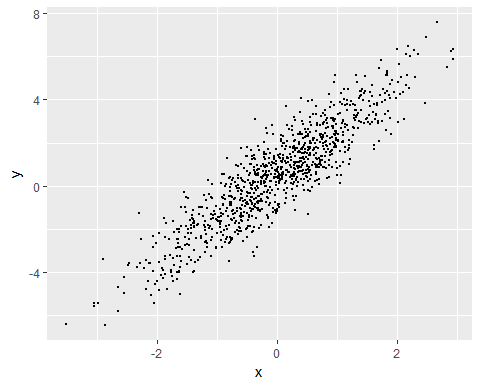
\includegraphics[width=0.6\linewidth]{ProcAnFinDataR_ed_1_files/figure-latex/unnamed-chunk-479-1} \end{center}

Clearly, there is a positive linear correlation; an upward straight line
would be a good approximation for the relationship between these
variables. We can check this result with the calculation of the
correlation coefficient with command
\texttt{cor(temp.df\$x,\ temp.df\$y)}. Here, the correlation between
\texttt{y} and \texttt{x} is 0.901.

\subsection{Estimating a Linear Model}\label{estimating-ols}

In R, the main function for estimating a linear model is \texttt{lm}.
Let's use it to estimate a model from the previous simulated data.
\index{base!lm}

\begin{Shaded}
\begin{Highlighting}[]
\CommentTok{# set df}
\NormalTok{lm.df <-}\StringTok{ }\KeywordTok{data.frame}\NormalTok{(x, y)}

\CommentTok{# estimate linear model}
\NormalTok{my.lm <-}\StringTok{ }\KeywordTok{lm}\NormalTok{(}\DataTypeTok{data =}\NormalTok{ lm.df, }\DataTypeTok{formula =}\NormalTok{ y }\OperatorTok{~}\StringTok{ }\NormalTok{x)}
\KeywordTok{print}\NormalTok{(my.lm)}
\end{Highlighting}
\end{Shaded}

\begin{verbatim}
## 
## Call:
## lm(formula = y ~ x, data = lm.df)
## 
## Coefficients:
## (Intercept)            x  
##      0.5083       1.9891
\end{verbatim}

The \texttt{formula} argument defines the shape of the linear model. If
we had another column, called \texttt{x2}, and wanted to include it in
the model, we could write
\texttt{formula=y\ \textasciitilde{}\ x1\ +\ x2}. Notice the intercept
(\(\alpha\)) is, by default, included in the estimation. If we needed to
omit the intercept, we could write
\texttt{formula=y\ \textasciitilde{}\ 0\ +\ x1} or
\texttt{formula=y\ \textasciitilde{}\ -1\ +\ x1}.

Argument \texttt{formula} allows other custom options, including
interactions between the explanatory variables. Let's create another
artificial dataset and look at some of these options:

\begin{Shaded}
\begin{Highlighting}[]
\KeywordTok{set.seed}\NormalTok{(}\DecValTok{15}\NormalTok{)}

\CommentTok{# set simulated dataset}
\NormalTok{N <-}\StringTok{ }\DecValTok{100}
\NormalTok{df <-}\StringTok{ }\KeywordTok{data.frame}\NormalTok{(}\DataTypeTok{x =} \KeywordTok{runif}\NormalTok{(N),}
                 \DataTypeTok{y =} \KeywordTok{runif}\NormalTok{(N),}
                 \DataTypeTok{z =} \KeywordTok{runif}\NormalTok{(N),}
                 \DataTypeTok{group =} \KeywordTok{sample}\NormalTok{(LETTERS[}\DecValTok{1}\OperatorTok{:}\DecValTok{3}\NormalTok{],}
\NormalTok{                                N,}
                                \DataTypeTok{replace =} \OtherTok{TRUE}\NormalTok{ ))}

\CommentTok{# Vanilla formula}
\CommentTok{#}
\CommentTok{# example: y ~ x + z}
\CommentTok{# model: y(t) = alpha + beta(1)*x(t) + beta(2)*z(t) + error(t)}
\NormalTok{my.formula <-}\StringTok{ }\NormalTok{y }\OperatorTok{~}\StringTok{ }\NormalTok{x }\OperatorTok{+}\StringTok{ }\NormalTok{z}
\KeywordTok{print}\NormalTok{(}\KeywordTok{lm}\NormalTok{(}\DataTypeTok{data =}\NormalTok{ df, }
         \DataTypeTok{formula =}\NormalTok{ my.formula))}
\end{Highlighting}
\end{Shaded}

\begin{verbatim}
## 
## Call:
## lm(formula = my.formula, data = df)
## 
## Coefficients:
## (Intercept)            x            z  
##     0.44971      0.14223     -0.03781
\end{verbatim}

\begin{Shaded}
\begin{Highlighting}[]
\CommentTok{# vannila formula with dummies}
\CommentTok{#}
\CommentTok{# example: y ~ group + x + z}
\CommentTok{# model: y(t) = alpha + beta(1)*D_1(t)+beta(2)*D_2(t) + }
\CommentTok{#               beta(3)*x(t) + beta(4)*z(t) + error(t)}
\CommentTok{# D_i(t) - dummy for group i}
\NormalTok{my.formula <-}\StringTok{ }\NormalTok{y }\OperatorTok{~}\StringTok{ }\NormalTok{group }\OperatorTok{+}\StringTok{ }\NormalTok{x }\OperatorTok{+}\StringTok{ }\NormalTok{z}
\KeywordTok{print}\NormalTok{(}\KeywordTok{lm}\NormalTok{(}\DataTypeTok{data =}\NormalTok{ df, }
         \DataTypeTok{formula =}\NormalTok{ my.formula))}
\end{Highlighting}
\end{Shaded}

\begin{verbatim}
## 
## Call:
## lm(formula = my.formula, data = df)
## 
## Coefficients:
## (Intercept)       groupB       groupC            x  
##     0.48309     -0.06397      0.01144      0.13511  
##           z  
##    -0.05156
\end{verbatim}

\begin{Shaded}
\begin{Highlighting}[]
\CommentTok{# Without intercept}
\CommentTok{#}
\CommentTok{# example: y ~ -1 + x + z}
\CommentTok{# model: y(t) = beta(1)*x(t) + beta(2)*z(t) + error(t)}
\NormalTok{my.formula <-}\StringTok{ }\NormalTok{y }\OperatorTok{~}\StringTok{ }\OperatorTok{-}\DecValTok{1} \OperatorTok{+}\StringTok{ }\NormalTok{x }\OperatorTok{+}\StringTok{ }\NormalTok{z}
\KeywordTok{print}\NormalTok{(}\KeywordTok{lm}\NormalTok{(}\DataTypeTok{data =}\NormalTok{ df, }
         \DataTypeTok{formula =}\NormalTok{ my.formula))}
\end{Highlighting}
\end{Shaded}

\begin{verbatim}
## 
## Call:
## lm(formula = my.formula, data = df)
## 
## Coefficients:
##      x       z  
## 0.5183  0.3133
\end{verbatim}

\begin{Shaded}
\begin{Highlighting}[]
\CommentTok{# Using combinations of variables}
\CommentTok{# example: y ~ x*z}
\CommentTok{# model: y(t) = alpha + beta(1)*x(t) + beta(2)*z(t) + }
\CommentTok{#               beta(3)*x(t)*z(t) + error(t)}
\NormalTok{my.formula <-}\StringTok{ }\NormalTok{y }\OperatorTok{~}\StringTok{ }\NormalTok{x}\OperatorTok{*}\NormalTok{z}
\KeywordTok{print}\NormalTok{(}\KeywordTok{lm}\NormalTok{(}\DataTypeTok{data =}\NormalTok{ df, }
         \DataTypeTok{formula =}\NormalTok{ my.formula))}
\end{Highlighting}
\end{Shaded}

\begin{verbatim}
## 
## Call:
## lm(formula = my.formula, data = df)
## 
## Coefficients:
## (Intercept)            x            z          x:z  
##     0.39827      0.22970      0.05129     -0.15464
\end{verbatim}

\begin{Shaded}
\begin{Highlighting}[]
\CommentTok{# Interacting variables}
\CommentTok{# example: y ~ x:group + z}
\CommentTok{# model: y(t) = alpha + beta(1)*z(t) + beta(2)*x(t)*D_1(t) + }
\CommentTok{#               beta(3)*x(t)*D_2(t) + beta(4)*x(t)*D_3(t) + }
\CommentTok{#               error(t)}
\CommentTok{# D_i(t) - dummy for group i}
\NormalTok{my.formula <-}\StringTok{ }\NormalTok{y }\OperatorTok{~}\StringTok{ }\NormalTok{x}\OperatorTok{:}\NormalTok{group }\OperatorTok{+}\StringTok{ }\NormalTok{z}
\KeywordTok{print}\NormalTok{(}\KeywordTok{lm}\NormalTok{(}\DataTypeTok{data =}\NormalTok{ df, }
         \DataTypeTok{formula =}\NormalTok{ my.formula))}
\end{Highlighting}
\end{Shaded}

\begin{verbatim}
## 
## Call:
## lm(formula = my.formula, data = df)
## 
## Coefficients:
## (Intercept)            z     x:groupA     x:groupB  
##     0.45995     -0.05105      0.16573      0.06271  
##    x:groupC  
##     0.20025
\end{verbatim}

The different options in the \texttt{formula} input allow a diversified
range of linear models. Using common mathematical operations, such as
\texttt{log(x)}, is also possible. More details about advanced uses of
\texttt{formula} input is available in the
\href{https://stat.ethz.ch/R-manual/R-devel/library/stats/html/formula.html}{manual}.

The output of function \texttt{lm} is an object similar to a
\texttt{list}. Therefore, its elements can be accessed using the
\texttt{\$} operator. Let's print all available names:

\begin{Shaded}
\begin{Highlighting}[]
\CommentTok{# print names in model}
\KeywordTok{print}\NormalTok{(}\KeywordTok{names}\NormalTok{(my.lm))}
\end{Highlighting}
\end{Shaded}

\begin{verbatim}
##  [1] "coefficients"  "residuals"     "effects"      
##  [4] "rank"          "fitted.values" "assign"       
##  [7] "qr"            "df.residual"   "xlevels"      
## [10] "call"          "terms"         "model"
\end{verbatim}

As you can see, there is a slot, called \texttt{coefficients}. Let's
check its contents.

\begin{Shaded}
\begin{Highlighting}[]
\KeywordTok{print}\NormalTok{(my.lm}\OperatorTok{$}\NormalTok{coefficients)}
\end{Highlighting}
\end{Shaded}

\begin{verbatim}
## (Intercept)           x 
##   0.5083045   1.9890616
\end{verbatim}

All coefficients are stored in \texttt{my.lm\$coefficients}. Its content
is a simple atomic vector that increases in length, according to the
number of explanatory variables in the model.

In our example of using \texttt{lm} with simulated data, the estimated
coefficients are close to the actual values of 0.5 and 2. Remember, in
the previous code, we set these values as
\texttt{my.alpha\ \textless{}-\ 0.5} and
\texttt{my.beta\ \textless{}-\ 2}.

Experienced researchers have probably noted, from the econometric point
of view, using function \texttt{print} in the output of \texttt{lm}
results in little information. Besides the values of the coefficients,
many other aspects of a linear model must be analyzed. In R, to obtain
more information about the previously estimated model, we use function
\texttt{summary}. See next. \index{base!summary}

\begin{Shaded}
\begin{Highlighting}[]
\KeywordTok{print}\NormalTok{(}\KeywordTok{summary}\NormalTok{(my.lm))}
\end{Highlighting}
\end{Shaded}

\begin{verbatim}
## 
## Call:
## lm(formula = y ~ x, data = lm.df)
## 
## Residuals:
##     Min      1Q  Median      3Q     Max 
## -3.0444 -0.6906 -0.0244  0.6807  3.2892 
## 
## Coefficients:
##             Estimate Std. Error t value Pr(>|t|)    
## (Intercept)  0.50830    0.03107   16.36   <2e-16 ***
## x            1.98906    0.03031   65.61   <2e-16 ***
## ---
## Signif. codes:  
## 0 '***' 0.001 '**' 0.01 '*' 0.05 '.' 0.1 ' ' 1
## 
## Residual standard error: 0.9824 on 998 degrees of freedom
## Multiple R-squared:  0.8118, Adjusted R-squared:  0.8116 
## F-statistic:  4305 on 1 and 998 DF,  p-value: < 2.2e-16
\end{verbatim}

The estimated coefficients have high \emph{T} values, and the model has
a outstanding fit of the data, with an adjusted \(R^2\) value of 0.8116.
This positive result is not surprising. The data was simulated in a
linear process, and the correlation was introduced artificially.

Additional information is available in the resulting object from
\texttt{summary}. Let's look at the names of the output:

\begin{Shaded}
\begin{Highlighting}[]
\NormalTok{my.summary <-}\StringTok{ }\KeywordTok{summary}\NormalTok{(my.lm)}
\KeywordTok{print}\NormalTok{(}\KeywordTok{names}\NormalTok{(my.summary))}
\end{Highlighting}
\end{Shaded}

\begin{verbatim}
##  [1] "call"          "terms"         "residuals"    
##  [4] "coefficients"  "aliased"       "sigma"        
##  [7] "df"            "r.squared"     "adj.r.squared"
## [10] "fstatistic"    "cov.unscaled"
\end{verbatim}

Each of these elements contains information that can be reported in a
estimation table. We could export the values of coefficients, T
statistics, and others to a spreadsheet tool and create a custom table
to report the results. This, however, is not suggested. In section
\ref{reporting-models}, we will discuss the best ways of reporting a
model using specialized packages.

Now, let's move to an example with real data. For that, we will estimate
the beta coefficient of a randomly selected stock. The beta
specification, also called market model, is given by:

\[ R _t = \alpha + \beta R_{M,t} + \epsilon _t\]

First, let's load the stock and SP500 data. \index{calculating beta}

\begin{Shaded}
\begin{Highlighting}[]
\CommentTok{# load stock data}
\KeywordTok{load}\NormalTok{(}\StringTok{'data/SP500-Stocks-WithRet.RData'}\NormalTok{)}

\CommentTok{# select rnd asset and filter data }
\KeywordTok{set.seed}\NormalTok{(}\DecValTok{10}\NormalTok{)}
\NormalTok{my.asset <-}\StringTok{ }\KeywordTok{sample}\NormalTok{(my.df}\OperatorTok{$}\NormalTok{ticker,}\DecValTok{1}\NormalTok{)}
\NormalTok{my.df.asset <-}\StringTok{ }\NormalTok{my.df[my.df}\OperatorTok{$}\NormalTok{ticker }\OperatorTok{==}\StringTok{ }\NormalTok{my.asset, ]}

\CommentTok{# load SP500 data}
\NormalTok{df.sp500 <-}\StringTok{ }\KeywordTok{read.csv}\NormalTok{(}\DataTypeTok{file =} \StringTok{'data/SP500.csv'}\NormalTok{, }
                     \DataTypeTok{colClasses =} \KeywordTok{c}\NormalTok{(}\StringTok{'Date'}\NormalTok{,}\StringTok{'numeric'}\NormalTok{))}

\CommentTok{# calculate return}
\NormalTok{df.sp500}\OperatorTok{$}\NormalTok{ret <-}\StringTok{ }\KeywordTok{calc.ret}\NormalTok{(df.sp500}\OperatorTok{$}\NormalTok{price)}

\CommentTok{# print datasets}
\KeywordTok{print}\NormalTok{(}\KeywordTok{nrow}\NormalTok{(my.df.asset))}
\end{Highlighting}
\end{Shaded}

\begin{verbatim}
## [1] 1761
\end{verbatim}

\begin{Shaded}
\begin{Highlighting}[]
\KeywordTok{print}\NormalTok{(}\KeywordTok{nrow}\NormalTok{(df.sp500))}
\end{Highlighting}
\end{Shaded}

\begin{verbatim}
## [1] 1801
\end{verbatim}

You can see the number of rows of the dataset for stock JEC doesn't
match the rows of the SP500 index. The dates of the different
\texttt{dataframes} are not synchronized. So, the first step is to add a
column in \texttt{my.df} with the returns of the market index. For that,
we use function \texttt{match} to find the indices that synchronize the
dates.

\begin{Shaded}
\begin{Highlighting}[]
\CommentTok{# find location of dates in df.sp500}
\NormalTok{idx <-}\StringTok{ }\KeywordTok{match}\NormalTok{(my.df.asset}\OperatorTok{$}\NormalTok{ref.date, df.sp500}\OperatorTok{$}\NormalTok{date)}

\CommentTok{# create column in my.df with sp500 returns}
\NormalTok{my.df.asset}\OperatorTok{$}\NormalTok{ret.sp500 <-}\StringTok{ }\NormalTok{df.sp500}\OperatorTok{$}\NormalTok{ret[idx]}
\end{Highlighting}
\end{Shaded}

As a start, let's create the scatter plot with the returns of the stock
and the market index, adding a linear trend.

\begin{Shaded}
\begin{Highlighting}[]
\KeywordTok{library}\NormalTok{(ggplot2)}

\NormalTok{p <-}\StringTok{ }\KeywordTok{ggplot}\NormalTok{(}\DataTypeTok{data =}\NormalTok{ my.df.asset, }\KeywordTok{aes}\NormalTok{(}\DataTypeTok{x=}\NormalTok{ret.sp500, }\DataTypeTok{y=}\NormalTok{ret))}
\NormalTok{p <-}\StringTok{ }\NormalTok{p }\OperatorTok{+}\StringTok{ }\KeywordTok{geom_point}\NormalTok{()}
\NormalTok{p <-}\StringTok{ }\NormalTok{p }\OperatorTok{+}\StringTok{ }\KeywordTok{geom_smooth}\NormalTok{(}\DataTypeTok{method =} \StringTok{'lm'}\NormalTok{)}
\KeywordTok{print}\NormalTok{(p)}
\end{Highlighting}
\end{Shaded}

\begin{center}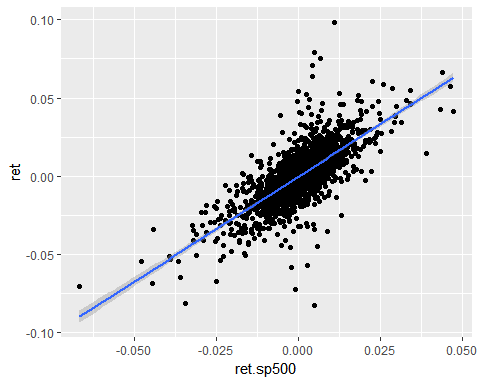
\includegraphics[width=0.6\linewidth]{ProcAnFinDataR_ed_1_files/figure-latex/unnamed-chunk-491-1} \end{center}

The figure shows a clear linear tendency; the returns from the market
index are a good predictor of the returns of the stock. Now, let's
estimate the linear model.

\begin{Shaded}
\begin{Highlighting}[]
\CommentTok{# estimate beta model}
\NormalTok{my.beta.model <-}\StringTok{ }\KeywordTok{lm}\NormalTok{(}\DataTypeTok{data =}\NormalTok{ my.df.asset, }\DataTypeTok{formula =}\NormalTok{ ret }\OperatorTok{~}\StringTok{ }\NormalTok{ret.sp500)}

\CommentTok{# print it}
\KeywordTok{print}\NormalTok{(}\KeywordTok{summary}\NormalTok{(my.beta.model))}
\end{Highlighting}
\end{Shaded}

\begin{verbatim}
## 
## Call:
## lm(formula = ret ~ ret.sp500, data = my.df.asset)
## 
## Residuals:
##       Min        1Q    Median        3Q       Max 
## -0.088660 -0.006393 -0.000273  0.006384  0.083767 
## 
## Coefficients:
##               Estimate Std. Error t value Pr(>|t|)    
## (Intercept) -0.0001985  0.0002920   -0.68    0.497    
## ret.sp500    1.3406720  0.0298163   44.96   <2e-16 ***
## ---
## Signif. codes:  
## 0 '***' 0.001 '**' 0.01 '*' 0.05 '.' 0.1 ' ' 1
## 
## Residual standard error: 0.01224 on 1759 degrees of freedom
## Multiple R-squared:  0.5348, Adjusted R-squared:  0.5345 
## F-statistic:  2022 on 1 and 1759 DF,  p-value: < 2.2e-16
\end{verbatim}

Previous output shows stock JEC has a beta equal to 1.34. This means
this is an aggressive stock with high sensitivity to market movements.

\subsection{Statistical Inference in Linear Models}\label{testing-ols}

After estimating a model with function \texttt{lm}, the next step is to
test some hypothesis about the coefficients. The F test verifies the
most basic condition for a model to justify its existence -- it tests
the assumption that all coefficients, excluding the intercept, are equal
to zero. When function \texttt{summary} is applied to a \texttt{lm}
output, the F-test is provided by default in the last line of the text
output. The null hypothesis of the test is that all slopes are equal to
zero. Let's try it:

\begin{verbatim}
## 
## Call:
## lm(formula = y ~ x.1 + x.2, data = df)
## 
## Residuals:
##      Min       1Q   Median       3Q      Max 
## -0.43125 -0.20631 -0.01184  0.18659  0.51744 
## 
## Coefficients:
##              Estimate Std. Error t value Pr(>|t|)    
## (Intercept)  0.449997   0.075048   5.996 3.46e-08 ***
## x.1         -0.004976   0.092259  -0.054    0.957    
## x.2         -0.006775   0.088308  -0.077    0.939    
## ---
## Signif. codes:  
## 0 '***' 0.001 '**' 0.01 '*' 0.05 '.' 0.1 ' ' 1
## 
## Residual standard error: 0.2621 on 97 degrees of freedom
## Multiple R-squared:  8.477e-05,  Adjusted R-squared:  -0.02053 
## F-statistic: 0.004112 on 2 and 97 DF,  p-value: 0.9959
\end{verbatim}

In this example, the F statistic is 0.0041119. The associated p-value is
higher than 10\%, indicating a strong statistical evidence in line with
the null hypothesis. We failed to reject the hypothesis that the
parameters attached to \texttt{x.1} and \texttt{x.2} are equal to zero.
The association between the explained variable and these vectors is
almost null. For an example with the rejection of the null hypothesis of
the F test, see the estimation of a model with artificial data in
section \ref{estimating-ols}.

Another type of test automatically executed by the \texttt{lm} and
\texttt{summary} function is the T test. While the F statistics test the
joint hypothesis that all coefficients are zero, the T statistic tests
it for individual parameters. It verifies the hypothesis that a specific
parameter is equal to zero. Each coefficient has its own T test.

In the practice of research, it is likely that both tests, T and F, will
suffice in most cases. They will give you information about the
statistical relationships in the data. However, you can also test custom
hypothesis, such as the sum or product of parameters equal to a
particular value, using package \texttt{car} \citep{car}. The tested
hypotheses are usually provided from a theoretical model or analysis.
For example, in section \ref{research-prophet}, we will study the
performance of a forecasting algorithm. We will test the performance of
the forecasts by estimating a linear model with the actual values of the
variable as dependent and the forecasts as independent (explanatory). If
the forecasting model works well, the intercept from the resulting model
should be zero, and the slope should be equal to one. We can jointly
test this hypothesis and calculate a p-value associated with it.

As a simple example, let's test a linear hypothesis for a simulated
model. Here, we will create artificial data and test the formal
hypothesis that the estimated coefficients are equal to the actual
values provided in the simulation.

\begin{Shaded}
\begin{Highlighting}[]
\KeywordTok{set.seed}\NormalTok{(}\DecValTok{10}\NormalTok{)}

\CommentTok{# number of time periods}
\NormalTok{nT <-}\StringTok{ }\DecValTok{1000}

\CommentTok{# set parameters}
\NormalTok{my.intercept <-}\StringTok{ }\FloatTok{0.5}
\NormalTok{my.beta <-}\StringTok{ }\FloatTok{1.5}

\CommentTok{# simulate}
\NormalTok{x <-}\StringTok{ }\KeywordTok{rnorm}\NormalTok{(nT)}
\NormalTok{y <-}\StringTok{ }\NormalTok{my.intercept }\OperatorTok{+}\StringTok{ }\NormalTok{my.beta}\OperatorTok{*}\NormalTok{x }\OperatorTok{+}\StringTok{ }\KeywordTok{rnorm}\NormalTok{(nT)}

\CommentTok{# set df}
\NormalTok{df <-}\StringTok{ }\KeywordTok{data.frame}\NormalTok{(y, x)}

\CommentTok{# estimate model}
\NormalTok{my.lm <-}\StringTok{ }\KeywordTok{lm}\NormalTok{(}\DataTypeTok{data =}\NormalTok{ df, }
            \DataTypeTok{formula =}\NormalTok{ y }\OperatorTok{~}\StringTok{ }\NormalTok{x )}
\end{Highlighting}
\end{Shaded}

After the estimation of the model, we use function
\texttt{LinearHypothesis} from package \texttt{car} \citep{car} to
implement our formal test. Before using it, we need to understand its
input. The first input, \texttt{model}, is the estimated model from the
previous chunk. Inputs \texttt{hypothesis.matrix} and \texttt{rhs}
determine the linear hypothesis of the test in a matrix format. The
object in \texttt{hypothesis.matrix} will be multiplied in matrix
notation by a vertical vector of the coefficients from the model. The
\texttt{rhs} (right hand side) determines the hypothesised result from
this calculation. In our case, the resulting matrix operation is:

\[  \underbrace{\begin{bmatrix}
1 & 0 \\ 
0 & 1
\end{bmatrix}}_{hypothesis.matrix}\begin{bmatrix}
\alpha \\
\beta
\end{bmatrix} = \underbrace{\begin{bmatrix}
0.5 \\ 
1.5  
\end{bmatrix} }_{rhs} \]

With this matrix operation, we test the joint hypothesis that the
intercept is equal to 0.5 and the slope is equivalent to 1.5. Notice
that using matrices gives flexibility to the user. We could test many
other linear hypotheses by changing the shape of
\texttt{hypothesis.matrix} and \texttt{rhs}. The actual R code that
implements the test is given next.

\begin{Shaded}
\begin{Highlighting}[]
\KeywordTok{library}\NormalTok{(car)}

\CommentTok{# set test matrix}
\NormalTok{test.matrix <-}\StringTok{ }\KeywordTok{matrix}\NormalTok{(}\KeywordTok{c}\NormalTok{(my.intercept,  }\CommentTok{# alpha test value}
\NormalTok{                        my.beta))  }\CommentTok{# beta test value}

\CommentTok{# hypothesis matrix }
\NormalTok{hyp.mat <-}\StringTok{ }\KeywordTok{matrix}\NormalTok{(}\KeywordTok{c}\NormalTok{(}\DecValTok{1}\NormalTok{,}\DecValTok{0}\NormalTok{,}
                    \DecValTok{0}\NormalTok{,}\DecValTok{1}\NormalTok{),}\DataTypeTok{nrow =} \DecValTok{2}\NormalTok{)}

\CommentTok{# do test}
\NormalTok{my.waldtest <-}\StringTok{ }\KeywordTok{linearHypothesis}\NormalTok{(my.lm, }
                                \DataTypeTok{hypothesis.matrix =}\NormalTok{ hyp.mat, }
                                \DataTypeTok{rhs =}\NormalTok{ test.matrix)}

\CommentTok{# print result}
\KeywordTok{print}\NormalTok{(my.waldtest)}
\end{Highlighting}
\end{Shaded}

\begin{verbatim}
## Linear hypothesis test
## 
## Hypothesis:
## (Intercept) = 0.5
## x = 1.5
## 
## Model 1: restricted model
## Model 2: y ~ x
## 
##   Res.Df    RSS Df Sum of Sq      F Pr(>F)
## 1   1000 1089.1                           
## 2    998 1086.8  2    2.3766 1.0912 0.3362
\end{verbatim}

As we can see, the test fails to reject the null hypothesis. This means
our simulation worked, and the parameters are correctly estimated as
expected.

Another family of tests commonly applied to linear models is related to
its assumptions. Every linear model of type OLS assumes several
conditions to its errors, including: 1) independence, 2)
homoscesdasticity (constant variance), and 3) adherence to the Normal
distribution. If these assumptions are not true, the model may be
inefficient or biased, meaning some modification or use of robust
estimates is required. More details about why these assumption must be
true and possible workarounds are found in any Econometric textbook,
such as \citet{greene2003econometric} and
\citet{maddala2001introduction}.

In R, we can use package \texttt{lmtest} \citep{lmtest} to test for
independence with the Breush-Godfrey and Durbin Watson test. The
Shapiro-Wilk test for normality is available in package \texttt{stats}.
Next, we provide an example of usage for the previously estimated model
with random data.

\begin{Shaded}
\begin{Highlighting}[]
\KeywordTok{library}\NormalTok{(lmtest)}

\CommentTok{# Breush Pagan test 1 - Serial correlation}
\CommentTok{# Null Hypothesis: No serial correlation in residual}
\KeywordTok{print}\NormalTok{(}\KeywordTok{bgtest}\NormalTok{(my.lm, }\DataTypeTok{order =} \DecValTok{5}\NormalTok{))}

\CommentTok{# Breush Pagan test 2 - Homocesdasticity of residuals}
\CommentTok{# Null Hypothesis: homocesdasticity }
\CommentTok{#                  (constant variance of residuals)}
\KeywordTok{print}\NormalTok{(}\KeywordTok{ncvTest}\NormalTok{(my.lm))}

\CommentTok{# Durbin Watson test - Serial correlation}
\CommentTok{# Null Hypothesis: No serial correlation in residual}
\KeywordTok{print}\NormalTok{(}\KeywordTok{dwtest}\NormalTok{(my.lm))}

\CommentTok{# Shapiro test  - Normality}
\CommentTok{# Null Hypothesis: Data is normally distributed}
\KeywordTok{print}\NormalTok{(}\KeywordTok{shapiro.test}\NormalTok{(my.lm}\OperatorTok{$}\NormalTok{residuals))}
\end{Highlighting}
\end{Shaded}

\begin{verbatim}
## 
##  Breusch-Godfrey test for serial correlation of order
##  up to 5
## 
## data:  my.lm
## LM test = 4.2628, df = 5, p-value = 0.5122
## 
## Non-constant Variance Score Test 
## Variance formula: ~ fitted.values 
## Chisquare = 1.54328    Df = 1     p = 0.2141302 
## 
##  Durbin-Watson test
## 
## data:  my.lm
## DW = 2.092, p-value = 0.9271
## alternative hypothesis: true autocorrelation is greater than 0
## 
## 
##  Shapiro-Wilk normality test
## 
## data:  my.lm$residuals
## W = 0.99803, p-value = 0.2964
\end{verbatim}

As expected, the model with artificial data passed all tests.

Another interesting approach for validating linear models is to use
package \texttt{gvlma} \citep{gvlma}. It provides a top level function
that can execute all sorts of tests in linear models, including the ones
described before. The main advantage is that it outputs all tests in a
single function call. Let's try it:

\begin{Shaded}
\begin{Highlighting}[]
\KeywordTok{library}\NormalTok{(gvlma)}

\CommentTok{# global validation of model}
\NormalTok{gvmodel <-}\StringTok{ }\KeywordTok{gvlma}\NormalTok{(my.lm) }

\CommentTok{# print result}
\KeywordTok{summary}\NormalTok{(gvmodel)}
\end{Highlighting}
\end{Shaded}

\begin{verbatim}
## 
## Call:
## lm(formula = y ~ x, data = df)
## 
## Residuals:
##     Min      1Q  Median      3Q     Max 
## -3.2703 -0.6898  0.0063  0.7346  3.8266 
## 
## Coefficients:
##             Estimate Std. Error t value Pr(>|t|)    
## (Intercept)  0.51510    0.03300   15.61   <2e-16 ***
## x            1.54658    0.03329   46.46   <2e-16 ***
## ---
## Signif. codes:  
## 0 '***' 0.001 '**' 0.01 '*' 0.05 '.' 0.1 ' ' 1
## 
## Residual standard error: 1.044 on 998 degrees of freedom
## Multiple R-squared:  0.6838, Adjusted R-squared:  0.6835 
## F-statistic:  2159 on 1 and 998 DF,  p-value: < 2.2e-16
## 
## 
## ASSESSMENT OF THE LINEAR MODEL ASSUMPTIONS
## USING THE GLOBAL TEST ON 4 DEGREES-OF-FREEDOM:
## Level of Significance =  0.05 
## 
## Call:
##  gvlma(x = my.lm) 
## 
##                     Value p-value                Decision
## Global Stat        3.6404  0.4569 Assumptions acceptable.
## Skewness           1.7814  0.1820 Assumptions acceptable.
## Kurtosis           0.1738  0.6767 Assumptions acceptable.
## Link Function      0.6628  0.4156 Assumptions acceptable.
## Heteroscedasticity 1.0224  0.3119 Assumptions acceptable.
\end{verbatim}

The output of \texttt{gvlma} shows several tests performed in the model.
The result is also positive, as the decision from the model is that the
OLS assumptions are acceptable. If a model did not pass the tests, one
solution is to use robust estimates of standard errors. Package
\texttt{sandwich} \citep{sandwich} offers function \texttt{NeweyWest}
for this purpose.

\section{Generalized Linear Models
(GLM)}\label{generalized-linear-models-glm}

The generalized linear model (GLM) is a flexible alternative to a linear
model. It allows the user to change the distribution of the error and
the link function, a systematic way that quantifies how the explained
variable will be affected by the response variable. GLM models are best
suited when the OLS assumptions, such as normality of residuals, don't
hold. For example, when you have a binary variable that takes only two
values and you want to write a model for it, the residual is not
normally distributed, given the limits of the explained variable.

We can write a general univariate GLM specification as:

\[ E \left( y _t \right) = g \left(\alpha + \sum ^N _{i=1} \beta _i x_{i,t}  \right)\]

The main difference of a GLM model and a OLS model is the use of a link
function \emph{g()} and a custom distribution assumption for the error
term. Function \emph{g()} can take many shapes. For example, if we are
modelling a binary variable, we can use \emph{g()} as the \emph{logit}
function:

\[ g(x) = \frac{\exp(x)}{1+\exp(x)} \]

Notice, in this case, function \emph{g()} ensures any value of \emph{x}
will result in a number between 0 and 1. The response of the explained
variable to the explanatory will be non linear.

\subsection{Simulating a GLM Model}\label{simulating-a-glm-model}

As an example, let's simulate the following GLM model, where the
response vector \(y_t\) is a Bernoulli variable that takes value 1 with
probability \(p_t\). The probabilities are calculated from the non
linear transformation of \(x_t\):

\[ p _t  = \frac{\exp(2+5x_t)}{1+\exp(2+5x_t)}  \]

In R, we use the following code to build the response vector.

\begin{Shaded}
\begin{Highlighting}[]
\KeywordTok{set.seed}\NormalTok{(}\DecValTok{15}\NormalTok{)}

\CommentTok{# set number of obs}
\NormalTok{nT <-}\StringTok{ }\DecValTok{500}

\CommentTok{# set x}
\NormalTok{x =}\StringTok{ }\KeywordTok{rnorm}\NormalTok{(nT)}

\NormalTok{my.alpha <-}\StringTok{ }\DecValTok{2}
\NormalTok{my.beta <-}\StringTok{ }\DecValTok{5}

\CommentTok{# set probabilities}
\NormalTok{z =}\StringTok{ }\NormalTok{my.alpha }\OperatorTok{+}\StringTok{ }\NormalTok{my.beta}\OperatorTok{*}\NormalTok{x}
\NormalTok{p =}\StringTok{ }\KeywordTok{exp}\NormalTok{(z)}\OperatorTok{/}\NormalTok{(}\DecValTok{1}\OperatorTok{+}\KeywordTok{exp}\NormalTok{(z))}

\CommentTok{# set response variable}
\NormalTok{y =}\StringTok{ }\KeywordTok{rbinom}\NormalTok{(}\DataTypeTok{n =}\NormalTok{ nT,}\DataTypeTok{size =} \DecValTok{1}\NormalTok{, }\DataTypeTok{prob =}\NormalTok{ p)}
\end{Highlighting}
\end{Shaded}

Function \texttt{rbinom} creates a vector of 1s and 0s, based on the
probabilities of input \texttt{prob}. Let's plot the simulated series
over time with \texttt{ggplot}.

\begin{Shaded}
\begin{Highlighting}[]
\KeywordTok{library}\NormalTok{(ggplot2)}

\CommentTok{# set df for ggplot}
\NormalTok{df =}\StringTok{ }\KeywordTok{data.frame}\NormalTok{(y, x)}

\CommentTok{# plot GLM sim}
\NormalTok{p <-}\StringTok{ }\KeywordTok{ggplot}\NormalTok{(}\DataTypeTok{data =}\NormalTok{ df, }\KeywordTok{aes}\NormalTok{(}\DataTypeTok{x=}\KeywordTok{seq_along}\NormalTok{(y) ,}\DataTypeTok{y=}\NormalTok{y))}
\NormalTok{p <-}\StringTok{ }\NormalTok{p }\OperatorTok{+}\StringTok{ }\KeywordTok{geom_point}\NormalTok{(}\DataTypeTok{size=}\FloatTok{0.5}\NormalTok{)}
\KeywordTok{print}\NormalTok{(p)}
\end{Highlighting}
\end{Shaded}

\begin{center}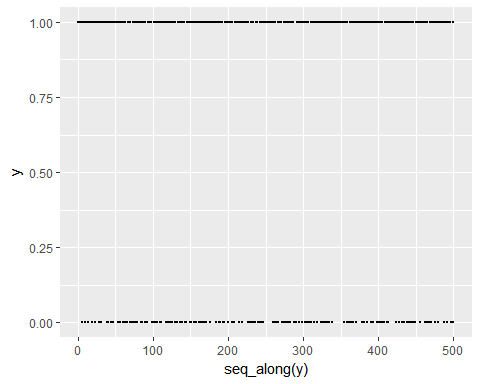
\includegraphics[width=0.6\linewidth]{ProcAnFinDataR_ed_1_files/figure-latex/unnamed-chunk-508-1} \end{center}

Object \texttt{y} contains zeros and ones, as expected.

\subsection{Estimating a GLM Model}\label{estimating-a-glm-model}

In R, the estimation of GLM models is accomplished with function
\texttt{glm}. It works similarly to \texttt{lm} but contains several
extra arguments that control the details of the models, such as the link
function and the distribution of the residuals.

First, let's use the previously simulated data to estimate a logit
model:

\begin{Shaded}
\begin{Highlighting}[]
\CommentTok{# estimate GLM}
\NormalTok{my.glm <-}\StringTok{ }\KeywordTok{glm}\NormalTok{(}\DataTypeTok{data=}\NormalTok{df, }
              \DataTypeTok{formula =}\NormalTok{ y}\OperatorTok{~}\NormalTok{x , }
              \DataTypeTok{family=} \KeywordTok{binomial}\NormalTok{(}\DataTypeTok{link =} \StringTok{"logit"}\NormalTok{))}

\CommentTok{# print it with summary}
\KeywordTok{print}\NormalTok{(}\KeywordTok{summary}\NormalTok{(my.glm))}
\end{Highlighting}
\end{Shaded}

\begin{verbatim}
## 
## Call:
## glm(formula = y ~ x, family = binomial(link = "logit"), data = df)
## 
## Deviance Residuals: 
##      Min        1Q    Median        3Q       Max  
## -2.99392  -0.13689   0.04087   0.23250   2.91383  
## 
## Coefficients:
##             Estimate Std. Error z value Pr(>|z|)    
## (Intercept)   2.1488     0.2622   8.197 2.47e-16 ***
## x             4.9050     0.5110   9.598  < 2e-16 ***
## ---
## Signif. codes:  
## 0 '***' 0.001 '**' 0.01 '*' 0.05 '.' 0.1 ' ' 1
## 
## (Dispersion parameter for binomial family taken to be 1)
## 
##     Null deviance: 634.18  on 499  degrees of freedom
## Residual deviance: 214.14  on 498  degrees of freedom
## AIC: 218.14
## 
## Number of Fisher Scoring iterations: 7
\end{verbatim}

The estimated coefficients are close to what we set in \texttt{my.alpha}
and \texttt{my.beta}. As expected, the model has a good fit of the data,
with both parameters being statistically significant at 1\%.

Function \texttt{glm} offers many options for setting a customized
model. From the help files, we have the following alternatives for the
distribution and link function and their corresponding inputs:

\begin{tabular}{l|l}
\hline
Family & Default Link Function\\
\hline
binomial & link = "logit"\\
\hline
gaussian & link = "identity"\\
\hline
Gamma & link = "inverse"\\
\hline
inverse.gaussian & link = "1/mu\textasciicircum{}2"\\
\hline
poisson & link = "log"\\
\hline
quasi & link = "identity", variance = "constant"\\
\hline
quasibinomial & link = "logit"\\
\hline
quasipoisson & link = "log"\\
\hline
\end{tabular}

The first step in using a GLM model is to identify the distribution and
link function that best suits your data. After that, you can use the
previous table to set the input of function \texttt{glm}.

As an example with real data from financial markets, let's randomly
select a stock and estimate a model for the probability of a positive
return with the probit model
(\texttt{link=\textquotesingle{}probit\textquotesingle{}}). We will use
the returns of the SP500 as the explanatory variable. We want to test
whether the market index influences the chance that a stock has a
positive return, an alternative version of the market model.

\begin{Shaded}
\begin{Highlighting}[]
\KeywordTok{set.seed}\NormalTok{(}\DecValTok{15}\NormalTok{)}

\CommentTok{# select stock}
\NormalTok{my.stock <-}\StringTok{ }\KeywordTok{sample}\NormalTok{(}\KeywordTok{unique}\NormalTok{(my.df}\OperatorTok{$}\NormalTok{ticker), }\DecValTok{1}\NormalTok{)}
\NormalTok{my.df.asset <-}\StringTok{ }\NormalTok{my.df[my.df}\OperatorTok{$}\NormalTok{ticker }\OperatorTok{==}\StringTok{ }\NormalTok{my.stock, ]}

\CommentTok{# find location of dates in df.sp500}
\NormalTok{idx <-}\StringTok{ }\KeywordTok{match}\NormalTok{(my.df.asset}\OperatorTok{$}\NormalTok{ref.date, df.sp500}\OperatorTok{$}\NormalTok{date)}

\CommentTok{# create column in my.df with sp500 returns}
\NormalTok{my.df.asset}\OperatorTok{$}\NormalTok{ret.sp500 <-}\StringTok{ }\NormalTok{df.sp500}\OperatorTok{$}\NormalTok{ret[idx]}

\CommentTok{# set column with dummy variable}
\NormalTok{my.df.asset}\OperatorTok{$}\NormalTok{D_ret <-}\StringTok{ }\NormalTok{my.df.asset}\OperatorTok{$}\NormalTok{ret }\OperatorTok{>}\StringTok{ }\DecValTok{0}

\CommentTok{# estimate model}
\NormalTok{my.glm <-}\StringTok{ }\KeywordTok{glm}\NormalTok{(}\DataTypeTok{data=}\NormalTok{my.df.asset,}
              \DataTypeTok{formula =}\NormalTok{ D_ret}\OperatorTok{~}\NormalTok{ret.sp500 , }
              \DataTypeTok{family=} \KeywordTok{binomial}\NormalTok{(}\DataTypeTok{link =} \StringTok{"probit"}\NormalTok{))}

\KeywordTok{print}\NormalTok{(}\KeywordTok{summary}\NormalTok{(my.glm))}
\end{Highlighting}
\end{Shaded}

\begin{verbatim}
## 
## Call:
## glm(formula = D_ret ~ ret.sp500, family = binomial(link = "probit"), 
##     data = my.df.asset)
## 
## Deviance Residuals: 
##     Min       1Q   Median       3Q      Max  
## -2.7100  -1.0391   0.2688   1.0161   2.5873  
## 
## Coefficients:
##              Estimate Std. Error z value Pr(>|z|)    
## (Intercept) -0.005122   0.032334  -0.158    0.874    
## ret.sp500   78.567162   4.616749  17.018   <2e-16 ***
## ---
## Signif. codes:  
## 0 '***' 0.001 '**' 0.01 '*' 0.05 '.' 0.1 ' ' 1
## 
## (Dispersion parameter for binomial family taken to be 1)
## 
##     Null deviance: 2439.8  on 1760  degrees of freedom
## Residual deviance: 2038.9  on 1759  degrees of freedom
## AIC: 2042.9
## 
## Number of Fisher Scoring iterations: 5
\end{verbatim}

The parameter for the market index is positive and significant. This
result implies the probability that stock MJN has a positive return is
affected by the changes in the SP500. When the index increases its
prices, a positive return in the stock is more likely.

\section{Panel Data Models}\label{panel-data-models}

Panel data models are advised when the modelled data is
multidimensional, covering information about individuals or companies
that spawn over time. A dataset with financial information about several
companies for many years is a classic case of panel data. We have a
column identifying the company, another column for the time, and one or
more columns identifying the financial indicators. In a cross section of
time, we have several companies and several financial ratios. The
dataset can be further categorized as balanced, where all companies have
information in all dates, and unbalanced, where not all companies have
data for all dates.

The main motivation to use panel data models is to allow common effects
within the groups. If a standard OLS estimation is used for each group,
such as companies, we implicitly assume the models are independent. If
the assumption of independence is not true, our econometric analysis is
jeopardized by a possible bias. Using panel data models allows for more
flexible representations. Some parameters can be individual to each
group, while others are shared. Using panel data models requires careful
thought about how the model is identified. Many statistical tests are
available for this purpose.

We can represent the simplest case of a panel data model as:

\[ y_{i,t} = \alpha _i + \beta x_{i,t}+\epsilon _{i,t} \]

Notice we now use index \emph{i} in the dependent and independent
variables. This index controls for the groups, such as different
companies. In our specific model, all \emph{i} cases have different
intercepts, but share the same beta. Depending on the assumptions about
the intercept, the previous equation can represent a panel data model of
type \emph{fixed} or \emph{random effects} . There are many other ways
to customize a panel data model and set dynamic effects, such as lagged
terms. You can find more details in \citet{hsiao2014analysis}.

\subsection{Simulating Panel Data
Models}\label{simulating-panel-data-models}

Let's simulate a balanced panel data with fixed effects for twelve
different firms and five time periods. This is a classic case of panel
data, with large \emph{N} and small \emph{T}. Each company will have a
explanatory variable, called \texttt{x}, that varies over different
dates. The following code uses matrix operations to simulate all cases.
Notice the many uses of the \texttt{sapply} function. After creating the
multivariate data, we stack it in single vectors and save it in a
\texttt{dataframe}.

\begin{Shaded}
\begin{Highlighting}[]
\KeywordTok{set.seed}\NormalTok{(}\DecValTok{25}\NormalTok{)}

\CommentTok{# number of obs for each case}
\NormalTok{nT <-}\StringTok{ }\DecValTok{5}

\CommentTok{# set number of groups}
\NormalTok{N <-}\StringTok{ }\DecValTok{12}

\CommentTok{# set possible cases}
\NormalTok{possible.cases <-}\StringTok{ }\NormalTok{LETTERS[}\DecValTok{1}\OperatorTok{:}\NormalTok{N]}

\CommentTok{# set parameters}
\NormalTok{my.alphas <-}\StringTok{ }\KeywordTok{seq}\NormalTok{(}\OperatorTok{-}\DecValTok{10}\NormalTok{,}\DecValTok{10}\NormalTok{,}\DataTypeTok{length.out =}\NormalTok{ N)}
\NormalTok{my.beta <-}\StringTok{ }\FloatTok{1.5}

\CommentTok{# set indep var (x) and dates}
\NormalTok{indep.var <-}\StringTok{ }\KeywordTok{sapply}\NormalTok{(}\KeywordTok{rep}\NormalTok{(nT,N), rnorm)}
\NormalTok{my.dates <-}\StringTok{ }\KeywordTok{Sys.Date}\NormalTok{() }\OperatorTok{+}\StringTok{ }\DecValTok{1}\OperatorTok{:}\NormalTok{nT}

\CommentTok{# create response matrix (y)}
\NormalTok{response.matrix <-}\StringTok{ }\KeywordTok{matrix}\NormalTok{(}\KeywordTok{rep}\NormalTok{(my.alphas,nT), }
                          \DataTypeTok{nrow =}\NormalTok{ nT, }
                          \DataTypeTok{byrow =} \OtherTok{TRUE}\NormalTok{) }\OperatorTok{+}\StringTok{ }
\StringTok{  }\NormalTok{indep.var}\OperatorTok{*}\NormalTok{my.beta }\OperatorTok{+}\StringTok{ }\KeywordTok{sapply}\NormalTok{(}\KeywordTok{rep}\NormalTok{(nT,N),rnorm, }\DataTypeTok{sd =} \FloatTok{0.25}\NormalTok{) }

\CommentTok{# set df}
\NormalTok{sim.df <-}\StringTok{ }\KeywordTok{data.frame}\NormalTok{(}\DataTypeTok{G =} \KeywordTok{as.character}\NormalTok{(}\KeywordTok{sapply}\NormalTok{(possible.cases, }
\NormalTok{                                             rep, }
                                             \DataTypeTok{times=}\NormalTok{nT )),}
                     \DataTypeTok{dates =} \KeywordTok{rep}\NormalTok{(my.dates, }\DataTypeTok{times=}\NormalTok{N),}
                     \DataTypeTok{y =} \KeywordTok{as.numeric}\NormalTok{(response.matrix),}
                     \DataTypeTok{x =} \KeywordTok{as.numeric}\NormalTok{(indep.var), }
                     \DataTypeTok{stringsAsFactors =} \OtherTok{FALSE}\NormalTok{)}

\CommentTok{# print result}
\KeywordTok{print}\NormalTok{(}\KeywordTok{str}\NormalTok{(sim.df))}
\end{Highlighting}
\end{Shaded}

\begin{verbatim}
## 'data.frame':    60 obs. of  4 variables:
##  $ G    : chr  "A" "A" "A" "A" ...
##  $ dates: Date, format: "2017-05-04" ...
##  $ y    : num  -10.68 -11.55 -11.74 -9.84 -11.96 ...
##  $ x    : num  -0.212 -1.042 -1.153 0.322 -1.5 ...
## NULL
\end{verbatim}

The result is a \texttt{dataframe} object with 60 rows and 4 columns. We
can look at the scatter plot of \texttt{x} and \texttt{y} for each firm
using \texttt{ggplot2}:

\begin{Shaded}
\begin{Highlighting}[]
\KeywordTok{library}\NormalTok{(ggplot2)}

\NormalTok{p <-}\StringTok{ }\KeywordTok{ggplot}\NormalTok{(sim.df, }\KeywordTok{aes}\NormalTok{(}\DataTypeTok{x=}\NormalTok{x, }\DataTypeTok{y=}\NormalTok{y))}
\NormalTok{p <-}\StringTok{ }\NormalTok{p }\OperatorTok{+}\StringTok{ }\KeywordTok{geom_point}\NormalTok{()}
\NormalTok{p <-}\StringTok{ }\NormalTok{p }\OperatorTok{+}\StringTok{ }\KeywordTok{facet_wrap}\NormalTok{(}\OperatorTok{~}\NormalTok{G)}

\KeywordTok{print}\NormalTok{(p)}
\end{Highlighting}
\end{Shaded}

\begin{center}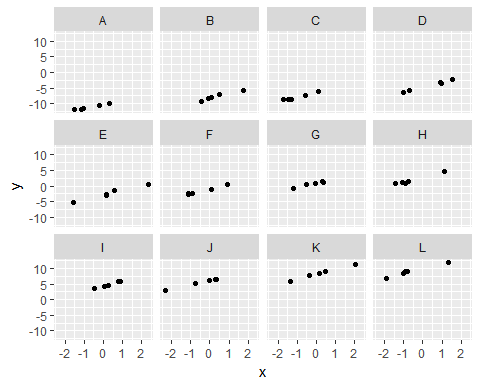
\includegraphics[width=0.6\linewidth]{ProcAnFinDataR_ed_1_files/figure-latex/unnamed-chunk-515-1} \end{center}

The figure shows the strong linear relationship shared between x and y
in the different groups. If we estimated a linear model from this data,
we would have to allow a different intercept for each group we find in
column \texttt{cases}.

\subsection{Estimating Panel Data
Models}\label{estimating-panel-data-models}

With the artificial data simulated in the previous step, let's estimate
the model using package \texttt{plm} \citep{plm}. This is a great
package that offers a comprehensive set of tools in testing and
estimating panel data models. The interface of function \texttt{plm} is
similar to \texttt{lm}. However, we need to define the panel data model
in argument \texttt{model} and the names of columns that define the
groups and time reference in input \texttt{index}. \index{plm}
\index{plm!plm}

\begin{Shaded}
\begin{Highlighting}[]
\KeywordTok{library}\NormalTok{(plm)}

\CommentTok{# estimate panel data model with fixed effects}
\NormalTok{my.pdm <-}\StringTok{ }\KeywordTok{plm}\NormalTok{(}\DataTypeTok{data =}\NormalTok{ sim.df, }
              \DataTypeTok{formula =}\NormalTok{ y }\OperatorTok{~}\StringTok{ }\NormalTok{x, }
              \DataTypeTok{model =} \StringTok{'within'}\NormalTok{,}
              \DataTypeTok{index =} \KeywordTok{c}\NormalTok{(}\StringTok{'G'}\NormalTok{,}\StringTok{'dates'}\NormalTok{))}

\CommentTok{# print result}
\KeywordTok{print}\NormalTok{(}\KeywordTok{summary}\NormalTok{(my.pdm,))}
\end{Highlighting}
\end{Shaded}

\begin{verbatim}
## Oneway (individual) effect Within Model
## 
## Call:
## plm(formula = y ~ x, data = sim.df, model = "within", index = c("G", 
##     "dates"))
## 
## Balanced Panel: n=12, T=5, N=60
## 
## Residuals :
##    Min. 1st Qu.  Median 3rd Qu.    Max. 
##  -0.440  -0.148  -0.033   0.154   0.479 
## 
## Coefficients :
##   Estimate Std. Error t-value  Pr(>|t|)    
## x 1.479366   0.035854  41.261 < 2.2e-16 ***
## ---
## Signif. codes:  
## 0 '***' 0.001 '**' 0.01 '*' 0.05 '.' 0.1 ' ' 1
## 
## Total Sum of Squares:    106.87
## Residual Sum of Squares: 2.871
## R-Squared:      0.97313
## Adj. R-Squared: 0.96627
## F-statistic: 1702.44 on 1 and 47 DF, p-value: < 2.22e-16
\end{verbatim}

As expected, the parameters were correctly retrieved from the data, with
a small difference from the actual value defined in \texttt{my.beta}.
Notice the different intercepts were not printed in the \texttt{summary}
output. We can retrieve them using function \texttt{fixef}:

\begin{Shaded}
\begin{Highlighting}[]
\KeywordTok{print}\NormalTok{(}\KeywordTok{fixef}\NormalTok{(my.pdm))}
\end{Highlighting}
\end{Shaded}

\begin{verbatim}
##           A           B           C           D           E 
## -10.0934047  -8.2435523  -6.3253831  -4.6552624  -2.8087407 
##           F           G           H           I           J 
##  -0.9794636   0.9609360   2.7568233   4.4134081   6.2113577 
##           K           L 
##   8.1880249  10.0337231
\end{verbatim}

Again, the simulated intercept values are close to the ones obtained
from the estimation.

As an example with real data, let's use the dataset from
\citet{grunfeld1958determinants}. This research paper studied the
components of corporate investments using data for ten companies for
twenty years. The data is available with package \texttt{plm}, and we
can load it with function \texttt{data}. Let's import it and look in its
content.

\begin{Shaded}
\begin{Highlighting}[]
\KeywordTok{library}\NormalTok{(plm)}

\CommentTok{# data from Grunfeld}
\KeywordTok{data}\NormalTok{(}\StringTok{"Grunfeld"}\NormalTok{)}

\CommentTok{# print it}
\KeywordTok{print}\NormalTok{(}\KeywordTok{str}\NormalTok{(Grunfeld))}
\end{Highlighting}
\end{Shaded}

\begin{verbatim}
## 'data.frame':    200 obs. of  5 variables:
##  $ firm   : int  1 1 1 1 1 1 1 1 1 1 ...
##  $ year   : int  1935 1936 1937 1938 1939 1940 1941 1942 1943 1944 ...
##  $ inv    : num  318 392 411 258 331 ...
##  $ value  : num  3078 4662 5387 2792 4313 ...
##  $ capital: num  2.8 52.6 156.9 209.2 203.4 ...
## NULL
\end{verbatim}

The \texttt{Grunfeld} dataset contains company information about gross
investment, market value, and capital (plant and equipment). The
\texttt{dataframe} is in the long format and ready to be used. In the
model, column \texttt{inv} is set as the dependent variable. Columns
\texttt{firm} and \texttt{year} are the index of panel data estimation.
The remaining columns, \texttt{value} and \texttt{capital}, are
explanatory variables. You can find more details about the Grunfeld
data, including information about different versions of the dataset and
its historical usage, in \citet{kleiber2010grunfeld}.

A note here is important; given its high number of time periods in
proportion to the number of firms, the Grunfeld data is best suited for
a more advanced econometric model of type SUR (seemly unrelated
regression). For educational purposes of learning R, we will explore
other types of panel models with this dataset . See
\citet{greene2003econometric} for more details.

First, let's explore the raw data by estimating a different OLS model
for each firm. This is also called the pooled model. We can use function
\texttt{by} with a custom function for this purpose (see chapter
\ref{programming} for details).

\begin{Shaded}
\begin{Highlighting}[]
\NormalTok{my.fct <-}\StringTok{ }\ControlFlowTok{function}\NormalTok{(df) \{}
  \CommentTok{# Estimates a linear model from Grunfeld data}
  \CommentTok{#}
  \CommentTok{# Args:}
  \CommentTok{#   df - dataframe from Grunfeld}
  \CommentTok{#}
  \CommentTok{# Returns:}
  \CommentTok{#   lm object}
  
\NormalTok{  my.model <-}\StringTok{ }\KeywordTok{lm}\NormalTok{(}\DataTypeTok{data =}\NormalTok{ df, }
                 \DataTypeTok{formula =}\NormalTok{ inv }\OperatorTok{~}\StringTok{  }\NormalTok{value }\OperatorTok{+}\StringTok{ }\NormalTok{capital)}
  
  \KeywordTok{return}\NormalTok{(my.model)}
\NormalTok{\}}

\CommentTok{# estimate model for each firm}
\NormalTok{my.l <-}\StringTok{ }\KeywordTok{by}\NormalTok{(Grunfeld, }
           \DataTypeTok{INDICES =}\NormalTok{ Grunfeld}\OperatorTok{$}\NormalTok{firm, }
           \DataTypeTok{FUN =}\NormalTok{ my.fct)}

\CommentTok{# print result}
\NormalTok{my.coefs <-}\StringTok{ }\KeywordTok{sapply}\NormalTok{(my.l, coef)}
\KeywordTok{print}\NormalTok{(my.coefs)}
\end{Highlighting}
\end{Shaded}

\begin{verbatim}
##                        1           2           3
## (Intercept) -149.7824533 -49.1983219 -9.95630645
## value          0.1192808   0.1748560  0.02655119
## capital        0.3714448   0.3896419  0.15169387
##                       4            5           6          7
## (Intercept) -6.18996051 22.707116014 -8.68554338 -4.4995344
## value        0.07794782  0.162377704  0.13145484  0.0875272
## capital      0.31571819  0.003101737  0.08537427  0.1237814
##                       8           9          10
## (Intercept) -0.50939018 -7.72283708 0.161518567
## value        0.05289413  0.07538794 0.004573432
## capital      0.09240649  0.08210356 0.437369190
\end{verbatim}

The results show a great discrepancy between the coefficients obtained
for each firm. This is especially true for the intercept value. It
ranges from -149.8 to 22.71. This result shows evidence it might be more
realistic to assume different coefficients for the different firms. We
can formally test this hypothesis with function \texttt{polltest} from
\texttt{plm}. It tests the null hypothesis that all coefficients are the
same across the cases, against the alternative hypothesis they are not.
Let's use it.

\begin{Shaded}
\begin{Highlighting}[]
\CommentTok{# test if all coef are the same across firms}
\NormalTok{my.pooltest <-}\StringTok{ }\KeywordTok{pooltest}\NormalTok{(inv}\OperatorTok{~}\NormalTok{value}\OperatorTok{+}\NormalTok{capital, }
                        \DataTypeTok{data =}\NormalTok{ Grunfeld, }
                        \DataTypeTok{model =} \StringTok{"pooling"}\NormalTok{)}

\CommentTok{# print result}
\KeywordTok{print}\NormalTok{(my.pooltest)}
\end{Highlighting}
\end{Shaded}

\begin{verbatim}
## 
##  F statistic
## 
## data:  inv ~ value + capital
## F = 27.749, df1 = 27, df2 = 170, p-value < 2.2e-16
## alternative hypothesis: unstability
\end{verbatim}

The high F test and small p-value suggest the rejection of the null
hypothesis. The evidence that the same coefficients can be applied to
all firms is minimal. The motivation for using panel data models for the
Grunfeld dataset is justified by the statistical test.

Before estimating the model, we need to understand which kind of panel
data model is best suited for the data. For simplicity, let's assume
only two possible choices, fixed or random effects. In both models, each
group has unobserved individual effects but share the same impact (beta)
of the observed explanatory variables. The difference between the models
is how the unobserved individual effect is perceived. Individual effects
are correlated to the explanatory variables in the fixed effect model,
while in the random effects, they are random variables. The correct
estimation of the model and econometric analysis will change according
to the underlying correlation structure. See
\citet{greene2003econometric} for more technical details about the
difference between fixed and random effects models.

We can test the model specification using package \texttt{plm}. Function
\texttt{phtest} executes the Hausman test
\citep{hausman1978specification}, a statistical procedure that tests the
null hypothesis that the best model is the random effects and not the
fixed effect. Let's try it for our data.

\begin{Shaded}
\begin{Highlighting}[]
\CommentTok{# set options for Hausman test}
\NormalTok{my.formula <-}\StringTok{ }\NormalTok{inv }\OperatorTok{~}\StringTok{ }\NormalTok{value }\OperatorTok{+}\StringTok{ }\NormalTok{capital}
\NormalTok{my.index <-}\StringTok{ }\KeywordTok{c}\NormalTok{(}\StringTok{'firm'}\NormalTok{,}\StringTok{'year'}\NormalTok{)}

\CommentTok{# do Hausman test}
\NormalTok{my.hausman.test <-}\StringTok{ }\KeywordTok{phtest}\NormalTok{(}\DataTypeTok{x =}\NormalTok{ my.formula, }
                          \DataTypeTok{data =}\NormalTok{ Grunfeld,}
                          \DataTypeTok{model =} \KeywordTok{c}\NormalTok{(}\StringTok{'within'}\NormalTok{, }\StringTok{'random'}\NormalTok{),}
                          \DataTypeTok{index =}\NormalTok{ my.index)}

\CommentTok{# print result}
\KeywordTok{print}\NormalTok{(my.hausman.test)}
\end{Highlighting}
\end{Shaded}

\begin{verbatim}
## 
##  Hausman Test
## 
## data:  my.formula
## chisq = 2.3304, df = 2, p-value = 0.3119
## alternative hypothesis: one model is inconsistent
\end{verbatim}

The p-value of 31.19\% is higher than an acceptable threshold of 10\%.
Therefore, we fail to reject the null hypothesis that the most efficient
panel data model is the random effects. We have strong statistical
evidence that a random effect model is better suited than a fixed effect
type for the Grunfeld dataset.

After identifying the model, let's estimate it using function
\texttt{plm}.

\begin{Shaded}
\begin{Highlighting}[]
\CommentTok{# set panel data model with random effects}
\NormalTok{my.model <-}\StringTok{ 'random'}
\NormalTok{my.formula <-}\StringTok{ }\NormalTok{inv }\OperatorTok{~}\StringTok{ }\NormalTok{value }\OperatorTok{+}\StringTok{ }\NormalTok{capital}
\NormalTok{my.index <-}\StringTok{ }\KeywordTok{c}\NormalTok{(}\StringTok{'firm'}\NormalTok{,}\StringTok{'year'}\NormalTok{)}

\CommentTok{# estimate it}
\NormalTok{my.pdm.random <-}\StringTok{ }\KeywordTok{plm}\NormalTok{(}\DataTypeTok{data =}\NormalTok{ Grunfeld, }
                     \DataTypeTok{formula =}\NormalTok{ my.formula, }
                     \DataTypeTok{model =}\NormalTok{ my.model,}
                     \DataTypeTok{index =}\NormalTok{ my.index)}

\CommentTok{# print result}
\KeywordTok{print}\NormalTok{(}\KeywordTok{summary}\NormalTok{(my.pdm.random))}
\end{Highlighting}
\end{Shaded}

\begin{verbatim}
## Oneway (individual) effect Random Effect Model 
##    (Swamy-Arora's transformation)
## 
## Call:
## plm(formula = my.formula, data = Grunfeld, model = my.model, 
##     index = my.index)
## 
## Balanced Panel: n=10, T=20, N=200
## 
## Effects:
##                   var std.dev share
## idiosyncratic 2784.46   52.77 0.282
## individual    7089.80   84.20 0.718
## theta:  0.8612  
## 
## Residuals :
##    Min. 1st Qu.  Median 3rd Qu.    Max. 
## -178.00  -19.70    4.69   19.50  253.00 
## 
## Coefficients :
##               Estimate Std. Error t-value Pr(>|t|)    
## (Intercept) -57.834415  28.898935 -2.0013  0.04674 *  
## value         0.109781   0.010493 10.4627  < 2e-16 ***
## capital       0.308113   0.017180 17.9339  < 2e-16 ***
## ---
## Signif. codes:  
## 0 '***' 0.001 '**' 0.01 '*' 0.05 '.' 0.1 ' ' 1
## 
## Total Sum of Squares:    2381400
## Residual Sum of Squares: 548900
## R-Squared:      0.7695
## Adj. R-Squared: 0.76716
## F-statistic: 328.837 on 2 and 197 DF, p-value: < 2.22e-16
\end{verbatim}

As expected, the coefficients are significant at 1\%. The adjustment of
the model is also high, with an adjusted R-Squared equal to 0.77. This
means a great proportion of the variation in the data was explained by
the model. The results from the panel data model indicate the value of
the firms and their current assets are positively related to the amount
of investments. Firms with higher market value and capital tend to
invest more.

As a last example of using R in panel models with the \texttt{Grunfeld}
data, let's estimate a SUR (seemingly unrelated regression) model, which
is best suited for this data. The SUR specification assumes the
different models for each group can be estimated individually, with a
correlation between the disturbances across models. It is best suited
when we have many time periods and few groups, such as in the
\texttt{Grunfeld} data.

Package \texttt{systemfit} offers a function with the same name for the
estimation of the SUR model. The first step in using \texttt{systemfit}
is to allocate the \texttt{Grunfeld} data to a specific
\texttt{data.frame} format with function \texttt{plm::pdata.frame}.
Let's try it.

\begin{Shaded}
\begin{Highlighting}[]
\KeywordTok{library}\NormalTok{(systemfit)}

\CommentTok{# set pdataframe}
\NormalTok{p.Grunfeld <-}\StringTok{ }\KeywordTok{pdata.frame}\NormalTok{(Grunfeld, }\KeywordTok{c}\NormalTok{( }\StringTok{"firm"}\NormalTok{, }\StringTok{"year"}\NormalTok{ ))}

\CommentTok{# estimate sur}
\NormalTok{my.SUR <-}\StringTok{ }\KeywordTok{systemfit}\NormalTok{(}\DataTypeTok{formula =}\NormalTok{ inv }\OperatorTok{~}\NormalTok{value }\OperatorTok{+}\StringTok{ }\NormalTok{capital,}
                    \DataTypeTok{method =}  \StringTok{"SUR"}\NormalTok{,}
                    \DataTypeTok{data =}\NormalTok{ p.Grunfeld)}
\KeywordTok{print}\NormalTok{(my.SUR)}
\end{Highlighting}
\end{Shaded}

\begin{verbatim}
## 
## systemfit results 
## method: SUR 
## 
## Coefficients:
##  1_(Intercept)       X1_value     X1_capital 10_(Intercept) 
##   -135.6061364      0.1138135      0.3861235      1.9893500 
##      X10_value    X10_capital  2_(Intercept)       X2_value 
##     -0.0161291      0.3768475    -10.9059829      0.1627658 
##     X2_capital  3_(Intercept)       X3_value     X3_capital 
##      0.3406261    -15.8959008      0.0349626      0.1257302 
##  4_(Intercept)       X4_value     X4_capital  5_(Intercept) 
##      1.8043270      0.0678437      0.3075528     26.4673602 
##       X5_value     X5_capital  6_(Intercept)       X6_value 
##      0.1274473      0.0119871     -6.1934512      0.1333107 
##     X6_capital  7_(Intercept)       X7_value     X7_capital 
##      0.0540052     -9.7701305      0.1134649      0.1281802 
##  8_(Intercept)       X8_value     X8_capital  9_(Intercept) 
##      3.1490972      0.0537015      0.0433622     -3.1568643 
##       X9_value     X9_capital 
##      0.0765949      0.0654245
\end{verbatim}

The output object \texttt{my.SUR} contains the estimation of all
equations, firm by firm. Using \texttt{print} is limited in this case;
it only shows the estimated coefficients. Function \texttt{summary}
provides more information, including the correlation structure between
the disturbances. But, its output is extensive and would fill several
pages of this book. We leave it as an exercise.

\section{Arima Models}\label{arima-models}

Using time series models is common in financial research. Arima is a
special model that uses the past of a time series to explain its own
future. Estimating an Arima model for stock returns can tell how the
returns today are related to past returns. In a forecasting horse race,
we can compare predictive performance of forecasting candidates against
an Arima model. If the proposed model works well, it should provide
forecasts with higher accuracy.

A simple example of an Arima model is defined by the following equation:

\[y _t = 0.5 y_{t-1} - 0.2 \epsilon _{t-1} + \epsilon _t\]

In this example, we have an ARIMA(AR = 1, D = 0, MA = 1) model without
the intercept. This specific notation informs the configuration of the
model and the number of used parameters. The first value in (1, 0, 1)
indicates the maximum \emph{lag} used in \(y_t\) in the right hand side
of the equation. The second value indicates the degree of
differentiation of the time series \citep{hamilton1994time}. If \(D=1\),
we use the first difference of \(y_t\) as the dependent variable. The
third component, \emph{MA}, shows the maximum \emph{lag} used for the
error of the model. This identification process can be arbitrary or not.
A common procedure is to search for the combination of AR, D, and MA
terms that maximizes an adjustment function, as shown in section
\ref{arima-estimating}.

\subsection{Simulating Arima Models}\label{simulating-arima-models}

First, let's simulate an Arima model using function \texttt{arima.sim}
from \texttt{stat}. This package is loaded by default, and we need not
source it with \texttt{library}. \index{stat!arima.sim}

\begin{Shaded}
\begin{Highlighting}[]
\KeywordTok{set.seed}\NormalTok{(}\DecValTok{1}\NormalTok{)}

\CommentTok{# set number of observations}
\NormalTok{my.n <-}\StringTok{ }\DecValTok{5000}

\CommentTok{# set model's parameters}
\NormalTok{my.model <-}\StringTok{ }\KeywordTok{list}\NormalTok{(}\DataTypeTok{ar =} \FloatTok{0.5}\NormalTok{, }\DataTypeTok{ma =} \OperatorTok{-}\FloatTok{0.1}\NormalTok{)}
\NormalTok{my.sd <-}\StringTok{ }\DecValTok{1}

\CommentTok{# simulate model}
\NormalTok{my.ts <-}\StringTok{ }\KeywordTok{arima.sim}\NormalTok{(}\DataTypeTok{n =}\NormalTok{ my.n, }
                   \DataTypeTok{model =}\NormalTok{ my.model , }
                   \DataTypeTok{sd =}\NormalTok{ my.sd)}
\end{Highlighting}
\end{Shaded}

We can look at the result of the simulation by creating a plot with the
artificial time series:

\begin{Shaded}
\begin{Highlighting}[]
\KeywordTok{library}\NormalTok{(ggplot2)}

\CommentTok{# set df}
\NormalTok{temp.df <-}\StringTok{ }\KeywordTok{data.frame}\NormalTok{(}\DataTypeTok{y =} \KeywordTok{unclass}\NormalTok{(my.ts), }
                      \DataTypeTok{date =} \KeywordTok{Sys.Date}\NormalTok{() }\OperatorTok{+}\StringTok{ }\DecValTok{1}\OperatorTok{:}\NormalTok{my.n)}

\NormalTok{p <-}\StringTok{ }\KeywordTok{ggplot}\NormalTok{(temp.df, }\KeywordTok{aes}\NormalTok{(}\DataTypeTok{x =}\NormalTok{ date, }\DataTypeTok{y =}\NormalTok{ y))}
\NormalTok{p <-}\StringTok{ }\NormalTok{p }\OperatorTok{+}\StringTok{ }\KeywordTok{geom_line}\NormalTok{(}\DataTypeTok{size=}\FloatTok{0.5}\NormalTok{)}

\KeywordTok{print}\NormalTok{(p)}
\end{Highlighting}
\end{Shaded}

\begin{center}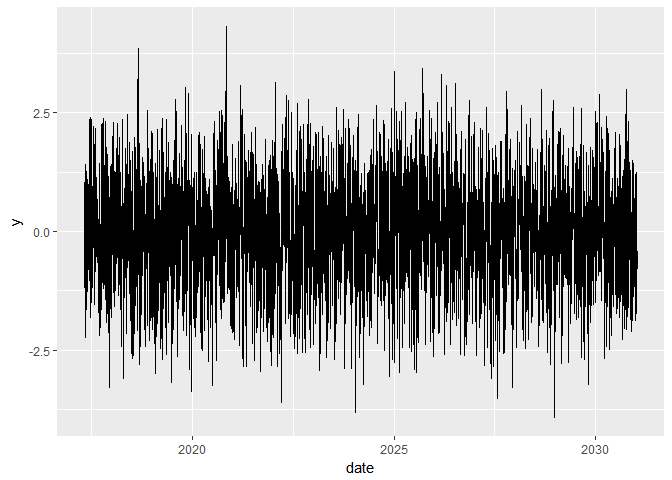
\includegraphics[width=0.6\linewidth]{ProcAnFinDataR_ed_1_files/figure-latex/unnamed-chunk-529-1} \end{center}

The graph shows a time series with an average close to zero and strong
instability. These are typical properties of an Arima model.

\subsection{Estimating Arima Models}\label{arima-estimating}

To estimate a Arima model, we use function \texttt{arima} from the same
package. Let's estimate a model for our simulated data.
\index{stat!arima}

\begin{Shaded}
\begin{Highlighting}[]
\CommentTok{# estimate arima model}
\NormalTok{my.arima <-}\StringTok{ }\KeywordTok{arima}\NormalTok{(my.ts, }\DataTypeTok{order =} \KeywordTok{c}\NormalTok{(}\DecValTok{1}\NormalTok{,}\DecValTok{0}\NormalTok{,}\DecValTok{1}\NormalTok{))}

\CommentTok{# print result}
\KeywordTok{print}\NormalTok{(}\KeywordTok{coef}\NormalTok{(my.arima))}
\end{Highlighting}
\end{Shaded}

\begin{verbatim}
##          ar1          ma1    intercept 
##  0.482547196 -0.077376754 -0.007458499
\end{verbatim}

As expected, the estimated parameters are close to the simulated values,
with \emph{ar1} equal to 0.4825 and \emph{ma1} equal to -0.07738. As we
did for a \texttt{lm} and \texttt{plm} model, we can also use function
\texttt{summary} to get more information from the estimation of the
Arima model. Let's look at all elements available in
\texttt{summary(my.arima)}: \index{base!summary}

\begin{Shaded}
\begin{Highlighting}[]
\KeywordTok{print}\NormalTok{(}\KeywordTok{summary}\NormalTok{(my.arima))}
\end{Highlighting}
\end{Shaded}

\begin{verbatim}
##           Length Class  Mode     
## coef         3   -none- numeric  
## sigma2       1   -none- numeric  
## var.coef     9   -none- numeric  
## mask         3   -none- logical  
## loglik       1   -none- numeric  
## aic          1   -none- numeric  
## arma         7   -none- numeric  
## residuals 5000   ts     numeric  
## call         3   -none- call     
## series       1   -none- character
## code         1   -none- numeric  
## n.cond       1   -none- numeric  
## nobs         1   -none- numeric  
## model       10   -none- list
\end{verbatim}

We have the adjustment criteria in \texttt{aic}, residuals in
\texttt{residuals}, coefficients in \texttt{coef}, covariance matrix of
estimated coefficients in \texttt{var.coef}, and many more.

The identification of the Arima model, defining values AR, D, MA in
Arima (AR, D, MA), can also be performed automatically. Package
\texttt{forecast} \citep{hyndman2007automatic} offers function
\texttt{auto.arima} that automates this process by choosing the best
model according to an adjustment criterion, such as AIC (\emph{Akaike
information criteria}) and BIC (\emph{Bayesian information criteria} ).
This is a very useful function. We allow the data to speak for itself,
avoiding a possible bias in the identification of the model.
\index{forecast!auto.arima}

In the next example, we use function \texttt{auto.arima} to find the
best model for the daily returns of the SP500 index. First, we load the
data from file \texttt{SP500.csv} and add a column for the returns using
function \texttt{calc.ret}, first presented in chapter
\ref{programming}.

\begin{Shaded}
\begin{Highlighting}[]
\CommentTok{# read file}
\NormalTok{my.f <-}\StringTok{ 'data/SP500.csv'}
\NormalTok{df.SP500 <-}\StringTok{ }\KeywordTok{read.csv}\NormalTok{(my.f)}

\NormalTok{calc.ret <-}\StringTok{ }\ControlFlowTok{function}\NormalTok{(P) \{}
  \CommentTok{# calculates arithmetic returns from a vector of prices}
  \CommentTok{#}
  \CommentTok{# Args:}
  \CommentTok{#   P - vector of prices (numeric)}
  \CommentTok{#}
  \CommentTok{# Returns:}
  \CommentTok{#   A vector of returns}
  
\NormalTok{  my.length <-}\StringTok{ }\KeywordTok{length}\NormalTok{(P)}
\NormalTok{  ret <-}\StringTok{ }\KeywordTok{c}\NormalTok{(}\OtherTok{NA}\NormalTok{, P[}\DecValTok{2}\OperatorTok{:}\NormalTok{my.length]}\OperatorTok{/}\NormalTok{P[}\DecValTok{1}\OperatorTok{:}\NormalTok{(my.length }\OperatorTok{-}\StringTok{ }\DecValTok{1}\NormalTok{)] }\OperatorTok{-}\StringTok{ }\DecValTok{1}\NormalTok{)}
  \KeywordTok{return}\NormalTok{(ret)}
\NormalTok{\}}

\CommentTok{# set return column}
\NormalTok{df.SP500}\OperatorTok{$}\NormalTok{ret <-}\StringTok{ }\KeywordTok{calc.ret}\NormalTok{(df.SP500}\OperatorTok{$}\NormalTok{price)}
\end{Highlighting}
\end{Shaded}

Before estimating the model, we need to check the stationarity of the
return data. If the data is not stationary, it might be necessary to use
the first differences of the original series
\citep{maddala2001introduction}. Since we are modelling returns, the raw
data of prices was already differentiated (see return equation in
chapter \ref{Financial-data}). It is worth testing this property of the
data before estimating the Arima model. Package \texttt{tseries}
\citep{tseries} provides a function called \texttt{adf.test} that will
check if the data has unit root (not stationary). The null hypothesis of
the test is the non-stationarity of the data, i.e, the existence of unit
roots. \index{tseries} \index{tseries!adf.test}

\begin{Shaded}
\begin{Highlighting}[]
\KeywordTok{library}\NormalTok{(tseries)}
\KeywordTok{print}\NormalTok{(}\KeywordTok{adf.test}\NormalTok{(}\KeywordTok{na.omit}\NormalTok{(df.SP500}\OperatorTok{$}\NormalTok{ret)))}
\end{Highlighting}
\end{Shaded}

\begin{verbatim}
## 
##  Augmented Dickey-Fuller Test
## 
## data:  na.omit(df.SP500$ret)
## Dickey-Fuller = -12.188, Lag order = 12, p-value =
## 0.01
## alternative hypothesis: stationary
\end{verbatim}

The result of the test shows a small p-value that strongly suggests the
rejection of the null hypothesis. The evidence indicates that the return
vector can be considered stationary. For curiosity, let's also try the
test on the price series:

\begin{Shaded}
\begin{Highlighting}[]
\KeywordTok{print}\NormalTok{(}\KeywordTok{adf.test}\NormalTok{(df.SP500}\OperatorTok{$}\NormalTok{price))}
\end{Highlighting}
\end{Shaded}

\begin{verbatim}
## 
##  Augmented Dickey-Fuller Test
## 
## data:  df.SP500$price
## Dickey-Fuller = -2.9396, Lag order = 12, p-value =
## 0.1806
## alternative hypothesis: stationary
\end{verbatim}

This time, we easily fail to reject the null hypothesis with a large
p-value. The test strongly suggests the price series is not stationary.
From the econometric point of view, we are correct in estimating an
Arima model for returns, not prices.

Function \texttt{forecast::auto.arima} estimates na Arima model with
automatic identification of the best model. Let's try it with its
default options:

\begin{Shaded}
\begin{Highlighting}[]
\KeywordTok{library}\NormalTok{(forecast)}

\CommentTok{# estimate arima model with automatic identification}
\NormalTok{my.autoarima <-}\StringTok{ }\KeywordTok{auto.arima}\NormalTok{(}\DataTypeTok{x =}\NormalTok{ df.SP500}\OperatorTok{$}\NormalTok{ret)}

\CommentTok{# print result}
\KeywordTok{print}\NormalTok{(my.autoarima)}
\end{Highlighting}
\end{Shaded}

\begin{verbatim}
## Series:  
## ARIMA(1,0,0) with non-zero mean 
## 
## Coefficients:
##           ar1   mean
##       -0.0499  5e-04
## s.e.   0.0235  2e-04
## 
## sigma^2 estimated as 9.373e-05:  log likelihood=5794.03
## AIC=-11582.06   AICc=-11582.05   BIC=-11565.58
\end{verbatim}

The result tells us the best model for the returns of the SP500 index is
an Arima (1,0,0). This result implies the return series of the financial
index has a low memory and only the previous return has predictable
power over the current returns. In this case, since we find a negative
coefficient, a positive return is more likely to be followed by a
negative return.

\subsection{Forecasting Arima Models}\label{forecasting-arima-models}

We can obtain the forecasts of an Arima model with function
\texttt{forecast}, also from package \texttt{forecast}. The forecast is
of the static type; only information up to time \emph{t} is used to make
forecasts in \emph{t+k}. In the following example, we calculate the
forecasts for 5 periods ahead, with their corresponding confidence
interval. \index{forecast!forecast}

\begin{Shaded}
\begin{Highlighting}[]
\CommentTok{# forecast model}
\KeywordTok{print}\NormalTok{(}\KeywordTok{forecast}\NormalTok{(my.autoarima, }\DataTypeTok{h =} \DecValTok{5}\NormalTok{))}
\end{Highlighting}
\end{Shaded}

\begin{verbatim}
##      Point Forecast       Lo 80      Hi 80       Lo 95
## 1802   0.0006066170 -0.01180036 0.01301359 -0.01836821
## 1803   0.0004481322 -0.01197427 0.01287054 -0.01855030
## 1804   0.0004560393 -0.01196641 0.01287848 -0.01854245
## 1805   0.0004556448 -0.01196680 0.01287809 -0.01854285
## 1806   0.0004556645 -0.01196678 0.01287811 -0.01854283
##           Hi 95
## 1802 0.01958145
## 1803 0.01944656
## 1804 0.01945453
## 1805 0.01945414
## 1806 0.01945416
\end{verbatim}

\section{Garch Models}\label{garch-models}

Garch models relate to the seminal work of
\citet{engle1982autoregressive} and \citet{bollerslev1986generalized}.
The main innovation in this class of models is that the variance of the
residual can change . This variation is modelled using a specific
autoregressive process. Garch models became very popular mainly because
they replicate characteristics of financial asset returns, such as the
existence of fat tails in their distribution and the clustering of
volatile periods, where extreme price movements happen within the same
time. Garch models are mostly used where risk is being assessed and
managed. \index{Garch models}

A GARCH model is modular. In its simplest format, you have two main
equations: a process that sets the conditional mean, and another that
defines the variance of the error. See the following example for an
ARIMA(1,0,0)-GARCH(1,1) model:

\[\begin{aligned} y _t &=  \mu + \theta y_{t-1} + \epsilon _t \\\epsilon _t &\sim N \left(0, h _t \right ) \\h _t &= \omega + \alpha \epsilon ^2 _{t-1}+ \beta h_{t-1} \end{aligned} \]

The \(y_t\) equation sets the process for the conditional mean, an AR
model with one lag. This is the actual observed value of the time
series. Variable \(h_t\) defines the variance of the error, the
instability of the model. Different Garch models will use different
equations for \(h_t\) and different distributions of the error term. In
its simplest case, the one presented here, we use the Normal
distribution. It is important to understand this basic notation for
Garch models, because R functions that handle this model follow the same
structure.

\subsection{Simulating Garch Models}\label{simulating-garch-models}

R has no native function to simulate and estimate models of Garch. There
are two main packages related to Garch models. The first is package
\texttt{fGarch} \citep{fgarch} and the second is \texttt{rugarch}
\citep{rugarch}. Both have great features and are optimized for agile
estimations. You will be well served in choosing either of them. For
simplicity, we will give preference to package \texttt{fGarch}, with an
interface similar to the one used with Arima models in the previous
section. \index{rugarch} \index{fGarch}

In \texttt{fGarch}, we simulate a model using function
\texttt{garchSim}. The first step is to load package \texttt{fGarch} and
create the model specification: \index{fGarch!garchSim}

\begin{Shaded}
\begin{Highlighting}[]
\KeywordTok{library}\NormalTok{(fGarch)}

\CommentTok{# set list with model spec}
\NormalTok{my.model =}\StringTok{ }\KeywordTok{list}\NormalTok{(}\DataTypeTok{omega=}\FloatTok{0.001}\NormalTok{, }
                \DataTypeTok{alpha=}\FloatTok{0.15}\NormalTok{, }
                \DataTypeTok{beta=}\FloatTok{0.8}\NormalTok{, }
                \DataTypeTok{mu=}\FloatTok{0.02}\NormalTok{, }
                \DataTypeTok{ar =} \FloatTok{0.1}\NormalTok{)}

\CommentTok{# set garch spec                }
\NormalTok{spec =}\StringTok{ }\KeywordTok{garchSpec}\NormalTok{(}\DataTypeTok{model =}\NormalTok{ my.model)}

\CommentTok{# print it}
\KeywordTok{print}\NormalTok{(spec)}
\end{Highlighting}
\end{Shaded}

\begin{verbatim}
## 
## Formula: 
##  ~ ar(1) + garch(1, 1)
## Model:
##  ar:    0.1
##  mu:    0.02
##  omega: 0.001
##  alpha: 0.15
##  beta:  0.8
## Distribution: 
##  norm
## Presample: 
##   time         z    h          y
## 1    0 0.1145392 0.02 0.02222222
\end{verbatim}

The previous code defines a Garch model equivalent to the following
equations.

\[\begin{aligned} y _t &=  0.02 + 0.1 y_{t-1} + \epsilon _t \\\epsilon _t &\sim N \left(0, h _t \right ) \\h _t &= 0.001 + 0.15 \epsilon ^2 _{t-1}+ 0.8 h_{t-1} \end{aligned} \]

To simulate \emph{1000} observations of this model, we use function
\texttt{garchSim}:

\begin{Shaded}
\begin{Highlighting}[]
\KeywordTok{set.seed}\NormalTok{(}\DecValTok{20}\NormalTok{)}
\CommentTok{# simulate garch model}
\NormalTok{sim.garch =}\StringTok{ }\KeywordTok{garchSim}\NormalTok{(spec, }\DataTypeTok{n =} \DecValTok{1000}\NormalTok{)}
\end{Highlighting}
\end{Shaded}

We can visualize the artificial time series generated by creating a plot
with \texttt{ggplot}:

\begin{Shaded}
\begin{Highlighting}[]
\CommentTok{# set df for ggplot}
\NormalTok{temp.df <-}\StringTok{ }\KeywordTok{data.frame}\NormalTok{(}\DataTypeTok{sim.ret =}\NormalTok{ sim.garch}\OperatorTok{$}\NormalTok{garch, }
                      \DataTypeTok{idx=}\KeywordTok{seq_along}\NormalTok{(sim.garch}\OperatorTok{$}\NormalTok{garch))}

\KeywordTok{library}\NormalTok{(ggplot2)}
\NormalTok{p <-}\StringTok{ }\KeywordTok{ggplot}\NormalTok{(temp.df, }\KeywordTok{aes}\NormalTok{(}\DataTypeTok{x=}\NormalTok{idx, }\DataTypeTok{y=}\NormalTok{sim.ret))}
\NormalTok{p <-}\StringTok{ }\NormalTok{p }\OperatorTok{+}\StringTok{ }\KeywordTok{geom_line}\NormalTok{()}
\KeywordTok{print}\NormalTok{(p)}
\end{Highlighting}
\end{Shaded}

\begin{center}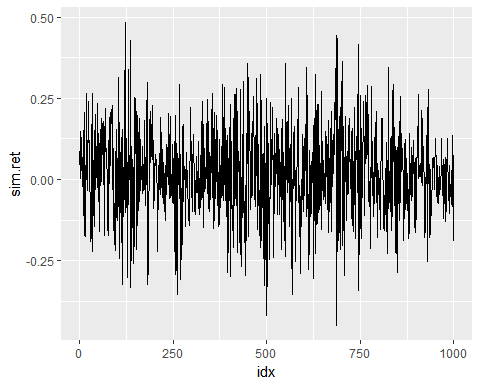
\includegraphics[width=0.6\linewidth]{ProcAnFinDataR_ed_1_files/figure-latex/unnamed-chunk-543-1} \end{center}

The behaviour of the simulated series is similar to the return series of
the stocks presented in chapter \ref{Figures}. It is difficult to set
one apart from the other based solely on visual inspection. Unlike other
models, where the instability is constant, a Garch model can portray a
return series more realistically by assuming a time changing volatility.

\subsection{Estimating Garch Models}\label{estimating-garch}

The estimation of the parameters from a GARCH model is usually achieved
using a technique called \emph{maximum-likelihood}. This procedure finds
the parameters that make the distribution of the model as close as
possible to the distribution of the time series of interest. It involves
a numerical optimization process that requires a reasonable amount of
processing time. Fortunately, package \texttt{fGarch} provides a
function, called \texttt{garchFit}, that performs the whole operation.
\index{fGarch!garchFit}

In the following example we estimate a Garch model for the artificial
data created in the previous section. We set option
\texttt{trace\ =\ FALSE} to prevent the presentation of the details of
the optimization process, as they are extensive and would occupy several
pages of this book.

\begin{Shaded}
\begin{Highlighting}[]
\CommentTok{# estimate garch model}
\NormalTok{my.garchfit <-}\StringTok{ }\KeywordTok{garchFit}\NormalTok{(}\DataTypeTok{data =}\NormalTok{ sim.garch, }
                        \DataTypeTok{formula =} \OperatorTok{~}\StringTok{ }\KeywordTok{arma}\NormalTok{(}\DecValTok{1}\NormalTok{,}\DecValTok{0}\NormalTok{) }\OperatorTok{+}\StringTok{ }\KeywordTok{garch}\NormalTok{(}\DecValTok{1}\NormalTok{,}\DecValTok{1}\NormalTok{), }
                        \DataTypeTok{trace =} \OtherTok{FALSE}\NormalTok{)}
\end{Highlighting}
\end{Shaded}

To learn more about the estimated model, we can present it on the screen
with the command \texttt{print}:

\begin{Shaded}
\begin{Highlighting}[]
\KeywordTok{print}\NormalTok{(my.garchfit)}
\end{Highlighting}
\end{Shaded}

\begin{verbatim}
## 
## Title:
##  GARCH Modelling 
## 
## Call:
##  garchFit(formula = ~arma(1, 0) + garch(1, 1), data = sim.garch, 
##     trace = FALSE) 
## 
## Mean and Variance Equation:
##  data ~ arma(1, 0) + garch(1, 1)
## <environment: 0x0000000005299a48>
##  [data = sim.garch]
## 
## Conditional Distribution:
##  norm 
## 
## Coefficient(s):
##        mu        ar1      omega     alpha1      beta1  
## 0.0164569  0.0695426  0.0010592  0.1292775  0.8175425  
## 
## Std. Errors:
##  based on Hessian 
## 
## Error Analysis:
##         Estimate  Std. Error  t value Pr(>|t|)    
## mu     0.0164569   0.0039213    4.197 2.71e-05 ***
## ar1    0.0695426   0.0327651    2.122   0.0338 *  
## omega  0.0010592   0.0004267    2.482   0.0131 *  
## alpha1 0.1292775   0.0282136    4.582 4.60e-06 ***
## beta1  0.8175425   0.0405741   20.149  < 2e-16 ***
## ---
## Signif. codes:  
## 0 '***' 0.001 '**' 0.01 '*' 0.05 '.' 0.1 ' ' 1
## 
## Log Likelihood:
##  604.1894    normalized:  0.6041894 
## 
## Description:
##  Wed May 03 15:22:40 2017 by user: marcelo
\end{verbatim}

The resulting parameters from the estimation are close to the values
defined arbitrarily in the call to \texttt{garchSpec}. We can achieve
higher accuracy by increasing the number of observations in the
simulated model. Function \texttt{summary} also works for Garch models.
Due to the large amount of information on the prompt, we leave it as an
exercise for the reader.

Now, as an example with real data, let's estimate a Garch model for the
SP500 index. The data is loaded from section \ref{arima-estimating}, so
we can use it directly. First, let's execute the LM Arch test
\citep{engle1982autoregressive, tsay2005analysis} to verify if the
returns of the market index have the Arch effect. Function
\texttt{ArchTest} from \texttt{FinTS} \citep{fints} can perform this
task. \index{FinTS} \index{FinTS!ArchTest}

\begin{Shaded}
\begin{Highlighting}[]
\KeywordTok{library}\NormalTok{(FinTS)}

\CommentTok{# test for Arch effects}
\NormalTok{my.arch.test <-}\StringTok{ }\KeywordTok{ArchTest}\NormalTok{(}\DataTypeTok{x =}\NormalTok{ df.SP500}\OperatorTok{$}\NormalTok{ret, }\DataTypeTok{lags =} \DecValTok{5}\NormalTok{)}

\CommentTok{# print result}
\KeywordTok{print}\NormalTok{(my.arch.test)}
\end{Highlighting}
\end{Shaded}

\begin{verbatim}
## 
##  ARCH LM-test; Null hypothesis: no ARCH effects
## 
## data:  df.SP500$ret
## Chi-squared = 357.05, df = 5, p-value < 2.2e-16
\end{verbatim}

The evidence is strong for Arch effects in SP500 returns. The null
hypothesis of the test is the non-existence of the Arch effects, and we
can easily reject it at 1\%. Let's estimate a Arma(1,0)-Garch(1,1) for
the returns.

\begin{Shaded}
\begin{Highlighting}[]
\CommentTok{# set object for estimation}
\NormalTok{df.est <-}\StringTok{ }\KeywordTok{as.timeSeries}\NormalTok{(}\KeywordTok{na.omit}\NormalTok{(df.SP500))}

\CommentTok{# estimate garch model for SP500}
\NormalTok{my.garchfit.sp500 <-}\StringTok{ }\KeywordTok{garchFit}\NormalTok{(}\DataTypeTok{data =}\NormalTok{ df.est , }
                              \DataTypeTok{formula =}\NormalTok{ ret }\OperatorTok{~}\StringTok{ }\KeywordTok{arma}\NormalTok{(}\DecValTok{1}\NormalTok{,}\DecValTok{0}\NormalTok{) }\OperatorTok{+}\StringTok{ }\KeywordTok{garch}\NormalTok{(}\DecValTok{1}\NormalTok{,}\DecValTok{1}\NormalTok{), }
                              \DataTypeTok{trace =} \OtherTok{FALSE}\NormalTok{)}

\KeywordTok{print}\NormalTok{(my.garchfit.sp500)}
\end{Highlighting}
\end{Shaded}

\begin{verbatim}
## 
## Title:
##  GARCH Modelling 
## 
## Call:
##  garchFit(formula = ret ~ arma(1, 0) + garch(1, 1), data = df.est, 
##     trace = FALSE) 
## 
## Mean and Variance Equation:
##  ret ~ arma(1, 0) + garch(1, 1)
##  [data = df.est]
## 
## Conditional Distribution:
##  norm 
## 
## Coefficient(s):
##          mu          ar1        omega       alpha1  
##  7.7257e-04  -4.4142e-02   4.1689e-06   1.5308e-01  
##       beta1  
##  8.0207e-01  
## 
## Std. Errors:
##  based on Hessian 
## 
## Error Analysis:
##          Estimate  Std. Error  t value Pr(>|t|)    
## mu      7.726e-04   1.749e-04    4.416 1.00e-05 ***
## ar1    -4.414e-02   2.616e-02   -1.687   0.0915 .  
## omega   4.169e-06   7.535e-07    5.533 3.15e-08 ***
## alpha1  1.531e-01   2.029e-02    7.544 4.55e-14 ***
## beta1   8.021e-01   2.220e-02   36.126  < 2e-16 ***
## ---
## Signif. codes:  
## 0 '***' 0.001 '**' 0.01 '*' 0.05 '.' 0.1 ' ' 1
## 
## Log Likelihood:
##  6040.208    normalized:  3.355671 
## 
## Description:
##  Wed May 03 15:22:41 2017 by user: marcelo
\end{verbatim}

As expected, all Garch coefficients are significant at 1\%. As for the
mean equation, we again find a negative value for \texttt{ar1}, but its
significance is not strong, with a p-value close to 10\%. We could use
the previously estimated Garch model to simulate future returns and
prices of the SP500 index.

\subsection{Forecasting Garch Models}\label{forecasting-garch-models}

Forecasting Garch models involves two elements: a forecast for the
conditional mean (see the first equation in the Garch formula) and a
forecast for future values of conditional volatility (see the second
equation). While the first sets the forecast of the next values of the
analysed series, the second quantifies the uncertainty of this forecast.

In package \texttt{fGarch}, both forecasts are calculated using function
\texttt{predict} that, just like \texttt{summary}, is a generic function
that can be used for different models. Consider the following example,
where we forecast the next values and the future volatilities of the
Garch model fitted with the SP500 returns. \index{fGarch!predict}

\begin{Shaded}
\begin{Highlighting}[]
\CommentTok{# static forecast for garch}
\NormalTok{my.garch.forecast <-}\StringTok{ }\KeywordTok{predict}\NormalTok{(my.garchfit.sp500, }\DataTypeTok{n.ahead =} \DecValTok{3}\NormalTok{)}

\CommentTok{# print df}
\KeywordTok{print}\NormalTok{(my.garch.forecast)}
\end{Highlighting}
\end{Shaded}

\begin{verbatim}
##   meanForecast   meanError standardDeviation
## 1 0.0008860155 0.005145661       0.005145661
## 2 0.0007334607 0.005432390       0.005427639
## 3 0.0007401948 0.005688981       0.005683925
\end{verbatim}

The first column of the previous result is the forecast of the
conditional mean; the second presents the expected error of the previous
forecast, and the third indicates the expected volatility in standard
deviation (root of the variance). All forecasts are the static type.
Information up to time \emph{t} is used to make forecasts for
\emph{t+k}.

\section{Regime Switching Models}\label{regime-switching-models}

Markov regime switching models are a specification in which the selling
point is the flexibility in handling processes driven by heterogeneous
states of the world \citep{hamilton:1994}. In financial markets, we can
have two regimes for volatility (uncertainty), one regime where
volatility is high and other where it is low. We can justify these
regimes as time periods with greater or lesser amount of new information
and uncertainty. Each regime can have its own characteristics. As a
modeller, we need to understand how to identify these regimes and
estimate the parameters from our models separately.

As a way to motivate the model, consider the following econometric
process:

\[ y_t=\mu_{S_t} + \epsilon_t \]

where \(S_t=1..k\) and \(\epsilon_t\) follows a Normal distribution with
zero mean and variance given by \(\sigma^2_{S_t}\). This is the simplest
case of a model with a switching dynamic. If there are \emph{k} states
of the world, there will be \emph{k} values for the conditional mean and
conditional variance. If there is only one state of the world
(\emph{k=1}), the previous formula becomes a simple linear regression
model under general conditions.

Now, let's assume the previous model has two states (\emph{k=2}). An
alternative representation is:

\begin{eqnarray*}
y_t=\mu_{1} + \epsilon_t \qquad \mbox{for State 1} \\
y_t=\mu_{2} + \epsilon_t \qquad \mbox{for State 2} 
\end{eqnarray*}

where:

\begin{eqnarray*}
\epsilon_t \sim (0,\sigma^2_{1}) \qquad \mbox{for State 1} \\
\epsilon_t \sim (0,\sigma^2_{2}) \qquad \mbox{for State 2} 
\end{eqnarray*}

This representation implies two processes for the dependent variable.
When the state of the world for time \emph{t} is 1, the expectation of
the dependent variable is \(\mu_1\) and the volatility of the
innovations is \(\sigma^2_1\). Likewise, when the state is 2, the mean
and volatility take other values.

As an example in finance, the dependent variable \(y_t\) can represent a
vector of log returns. The value of \(\mu_{1}\) is the expected return
on a bull market state, which implies a positive trend for financial
prices and consequently a positive log return. The lower, and possibly
negative, value of \(\mu_{2}\) measures the expected log return for the
bear market state, where asset prices have a tendency to go down.

The different volatilities represent the higher uncertainty regarding
the predictive power of the model in each state of the world. We can
expect the bear market state is more volatile than the bull market. This
implies prices go down faster than they go up. The usual explanation for
this effect is that traders react faster to bad news when comparing to
good news. This can also be explained by limit loss orders, which will
sell at market prices once a particular threshold in the prices has been
breached. When used by a significant amount of traders and at different
threshold levels, these limit loss orders will create a cascade effect,
accelerating the downfall of prices. This means we can expect the
volatility in state 2 (bear market) to be higher than the volatility in
state 1 (bull market).

The changes of the states in the model can be set in a deterministic
way. We could've set state 1 to be true for time \emph{t} when another
time series is higher or lower than a known threshold. This greatly
simplifies the model as each state is observable; therefore, we can
treat the model as a regression with dummy variables. Function
\texttt{lm} could be used for the estimation of this model.

A special regime switching model is markov switching. Its main
difference from the regression with dummy variables is the
identification of states is part of the estimation process. The model
learns it from the data. The transition of states in a markov switching
model is not deterministic; it is stochastic. This means one is never
sure whether there will be a switch of state. But, the dynamics behind
the switching process are known and driven by a transition matrix. This
matrix, also estimated from the data, will control the probabilities of
making a switch from one state to the other. It can be represented as:

\begin{equation*}
P=\left[ \begin{array}{ccc}
p_{11} & \ldots & p_{1k} \\
\vdots & \ddots & \vdots \\
p_{k1} & \ldots & p_{kk} \\
\end{array} \right ]        
\end{equation*}

In the previous matrix, row \emph{i}, column \emph{j} controls the
probability of a switch from state \emph{j} to state \emph{i}. Consider
that, for some time \emph{t}, the state of the world is 2. This means
the probability of a switch from state 2 to state 1 between time
\emph{t} and \emph{t+1} will be given by \(p_{12}\). Likewise, the
probability of staying in state 2 is determined by \(p_{22}\). This is
one of the central points of the structure of a markov regime switching
model: the switching of states is a stochastic process.

\subsection{Simulating Regime Switching
Models}\label{simulating-regime-switching-models}

In R, two packages are available for handling univariate markov regime
switching models, \texttt{MSwM} \citep{mswm} and
\texttt{fMarkovSwitching} \citep{fmarkovswitching}. The last one also
includes functions for simulating a time series. Before using it, let's
install \texttt{fMarkovSwitching} from the R-Forge repository. Be aware
this package is not available in CRAN.

\begin{Shaded}
\begin{Highlighting}[]
\KeywordTok{install.packages}\NormalTok{(}\StringTok{"fMarkovSwitching"}\NormalTok{, }
                 \DataTypeTok{repos=}\StringTok{"http://R-Forge.R-project.org"}\NormalTok{)}
\end{Highlighting}
\end{Shaded}

Once it is installed, let's look at its functions:

\begin{Shaded}
\begin{Highlighting}[]
\KeywordTok{library}\NormalTok{(fMarkovSwitching)}
\KeywordTok{print}\NormalTok{(}\KeywordTok{ls}\NormalTok{(}\StringTok{'package:fMarkovSwitching'}\NormalTok{))}
\end{Highlighting}
\end{Shaded}

\begin{verbatim}
## [1] "dim.MS_Model"     "MS_Regress_Fit"   "MS_Regress_For"  
## [4] "MS_Regress_Lik"   "MS_Regress_Simul" "plot.MS_Model"   
## [7] "plot.MS_Simul"    "print.MS_Model"   "print.MS_Simul"
\end{verbatim}

The package includes functions for simulating, estimating, and
forecasting an univariate markov switching model. As an example, let's
simulate the regime switching model from the following equations:

\begin{align*}
y_{t}&= +0.5x_t+\epsilon_{t} \qquad \mbox{State 1} \\
y_{t}&=-0.5x_t+\epsilon_{t} \qquad \mbox{State 2} \\
\epsilon _t &\sim N(0,0.25) \qquad \mbox{State 1} \\
\epsilon _t &\sim N(0,1) \qquad \mbox{State 2}
\end{align*}

The transition matrix will be given by:

\[
P=\left[ \begin{array}{ccc}
0.90 & 0.2 \\
0.10 & 0.8
\end{array} \right ]
\]

This model has two states with different volatilities. In each state,
the impact of the explanatory variable will be different. From package
\texttt{fMarkovSwitching}, we can use function
\texttt{MS\_Regress\_Simul} to simulate this model. Look at the
following code, where we simulate the model from the previous equations.

\begin{Shaded}
\begin{Highlighting}[]
\KeywordTok{set.seed}\NormalTok{(}\DecValTok{10}\NormalTok{)}
\KeywordTok{library}\NormalTok{(fMarkovSwitching)}

\CommentTok{# number of obs}
\NormalTok{nr <-}\StringTok{ }\DecValTok{500} 

\CommentTok{# distribution of residuals}
\NormalTok{distrib <-}\StringTok{ "Normal"} 

\CommentTok{# number of states}
\NormalTok{k <-}\StringTok{ }\DecValTok{2}  

\CommentTok{# set transition matrix}
\NormalTok{P <-}\StringTok{ }\KeywordTok{matrix}\NormalTok{(}\KeywordTok{c}\NormalTok{(.}\DecValTok{9}\NormalTok{ ,.}\DecValTok{2}\NormalTok{,}
\NormalTok{              .}\DecValTok{1}\NormalTok{ ,.}\DecValTok{8}\NormalTok{), }
            \DataTypeTok{nrow =} \DecValTok{2}\NormalTok{, }
            \DataTypeTok{byrow =}\NormalTok{ T)}

\CommentTok{# set switching flag           }
\NormalTok{S <-}\StringTok{ }\KeywordTok{c}\NormalTok{(}\DecValTok{0}\NormalTok{,}\DecValTok{1}\NormalTok{)}

\CommentTok{# set parameters of model (see manual for details)}
\NormalTok{nS_param <-}\StringTok{ }\KeywordTok{matrix}\NormalTok{(}\DecValTok{0}\NormalTok{)    }
\NormalTok{S_param <-}\StringTok{ }\KeywordTok{matrix}\NormalTok{(}\DecValTok{0}\NormalTok{,}\KeywordTok{sum}\NormalTok{(S),k)}
\NormalTok{S_param[,}\DecValTok{1}\NormalTok{] <-}\StringTok{  }\NormalTok{.}\DecValTok{5}         
\NormalTok{S_param[,}\DecValTok{2}\NormalTok{] <-}\StringTok{ }\OperatorTok{-}\NormalTok{.}\DecValTok{5}

\CommentTok{# set variance of model}
\NormalTok{sigma <-}\StringTok{ }\KeywordTok{matrix}\NormalTok{(}\DecValTok{0}\NormalTok{,}\DecValTok{1}\NormalTok{,k)}
\NormalTok{sigma[}\DecValTok{1}\NormalTok{,}\DecValTok{1}\NormalTok{] <-}\StringTok{ }\KeywordTok{sqrt}\NormalTok{(}\FloatTok{0.25}\NormalTok{)  }\CommentTok{# state 1}
\NormalTok{sigma[}\DecValTok{1}\NormalTok{,}\DecValTok{2}\NormalTok{] <-}\StringTok{ }\DecValTok{1}           \CommentTok{# state 2}

\CommentTok{# build list}
\NormalTok{Coeff <-}\StringTok{ }\KeywordTok{list}\NormalTok{(}\DataTypeTok{P =}\NormalTok{ P               ,}
              \DataTypeTok{S =}\NormalTok{ S               ,}
              \DataTypeTok{nS_param =}\NormalTok{ nS_param ,}
              \DataTypeTok{S_param =}\NormalTok{ S_param   ,}
              \DataTypeTok{sigma =}\NormalTok{ sigma       )}

\CommentTok{# simulate model}
\NormalTok{my.ms.simul <-}\StringTok{ }\KeywordTok{MS_Regress_Simul}\NormalTok{(nr,Coeff,k,distrib)}
\end{Highlighting}
\end{Shaded}

In the simulation function, argument \texttt{nS\_param} sets the non
switching parameters. These are the coefficients in the right hand side
of the econometric equation that will not switch states. We use a value
of zero, as our simulated model has no non-switching coefficients. Even
if not used, we need to set this argument in
\texttt{MS\_Regress\_Simul}; otherwise, the function will return an
error. The elements in \texttt{S\_param} define the coefficients in each
state for the switching parameters. In our example, we have a positive
effect of \(x_t\) in \(y_t\) in state one and a negative effect in state
two. Finally, the \texttt{sigma} input defines the volatility (standard
deviation) of the residual in each regime.

Once the model is simulated and available, let's plot the time series of
artificial values. A note here is important; the output from
\texttt{my.ms.simul} is a \texttt{S3} object was custom designed to
interact with the common functions \texttt{print} and \texttt{plot}. To
access its elements, we use \texttt{@} instead of \texttt{\$}.

\begin{Shaded}
\begin{Highlighting}[]
\KeywordTok{library}\NormalTok{(ggplot2)}
\NormalTok{df.to.plot <-}\StringTok{ }\KeywordTok{data.frame}\NormalTok{(}\DataTypeTok{y =}\NormalTok{ my.ms.simul}\OperatorTok{@}\NormalTok{dep, }
                         \DataTypeTok{x =} \KeywordTok{Sys.Date}\NormalTok{()}\OperatorTok{+}\DecValTok{1}\OperatorTok{:}\NormalTok{my.ms.simul}\OperatorTok{@}\NormalTok{nr,}
                         \DataTypeTok{states =}\NormalTok{ my.ms.simul}\OperatorTok{@}\NormalTok{trueStates[,}\DecValTok{1}\NormalTok{])}

\NormalTok{p <-}\StringTok{ }\KeywordTok{ggplot}\NormalTok{(}\DataTypeTok{data =}\NormalTok{ df.to.plot, }\KeywordTok{aes}\NormalTok{(}\DataTypeTok{y=}\NormalTok{y, }\DataTypeTok{x=}\KeywordTok{seq_along}\NormalTok{(y)))}
\NormalTok{p <-}\StringTok{ }\NormalTok{p }\OperatorTok{+}\StringTok{ }\KeywordTok{geom_line}\NormalTok{()}
\NormalTok{p <-}\StringTok{ }\NormalTok{p }\OperatorTok{+}\StringTok{ }\KeywordTok{labs}\NormalTok{(}\DataTypeTok{x=}\StringTok{'Time'}\NormalTok{, }\DataTypeTok{y =} \StringTok{'Simulated time series'}\NormalTok{)}
\KeywordTok{print}\NormalTok{(p)}
\end{Highlighting}
\end{Shaded}

\begin{center}\includegraphics[width=0.6\linewidth]{ProcAnFinDataR_ed_1_files/figure-latex/unnamed-chunk-564-1} \end{center}

We can also look at the simulated states:

\begin{Shaded}
\begin{Highlighting}[]
\KeywordTok{library}\NormalTok{(ggplot2)}
\NormalTok{df.to.plot <-}\StringTok{ }\KeywordTok{data.frame}\NormalTok{(}\DataTypeTok{y =}\NormalTok{ my.ms.simul}\OperatorTok{@}\NormalTok{dep, }
                         \DataTypeTok{x =} \KeywordTok{Sys.Date}\NormalTok{()}\OperatorTok{+}\DecValTok{1}\OperatorTok{:}\NormalTok{my.ms.simul}\OperatorTok{@}\NormalTok{nr,}
                         \DataTypeTok{states =}\NormalTok{ my.ms.simul}\OperatorTok{@}\NormalTok{trueStates[,}\DecValTok{1}\NormalTok{])}

\NormalTok{p <-}\StringTok{ }\KeywordTok{ggplot}\NormalTok{(}\DataTypeTok{data =}\NormalTok{ df.to.plot, }\KeywordTok{aes}\NormalTok{(}\DataTypeTok{y=}\NormalTok{states, }\DataTypeTok{x=}\NormalTok{x))}
\NormalTok{p <-}\StringTok{ }\NormalTok{p }\OperatorTok{+}\StringTok{ }\KeywordTok{geom_line}\NormalTok{()}
\NormalTok{p <-}\StringTok{ }\NormalTok{p }\OperatorTok{+}\StringTok{ }\KeywordTok{labs}\NormalTok{(}\DataTypeTok{y=}\StringTok{'Probability of state 1'}\NormalTok{)}
\KeywordTok{print}\NormalTok{(p)}
\end{Highlighting}
\end{Shaded}

\begin{center}\includegraphics[width=0.6\linewidth]{ProcAnFinDataR_ed_1_files/figure-latex/unnamed-chunk-565-1} \end{center}

As expected, the model is switching from one state to the other. Either
state is strongly predominant over time, but state one seems to have a
longer duration than state two. This property is controlled by the
transition probabilities set in object \texttt{P}.

\subsection{Estimating Regime Switching
Models}\label{estimating-regime-switching-models}

We can estimate a univariate markov switching model with function
\texttt{MS\_Regress\_Fit}. Let's try it for the previously simulated
time series.

\begin{Shaded}
\begin{Highlighting}[]
\CommentTok{# set dep and indep }
\NormalTok{dep <-}\StringTok{ }\NormalTok{my.ms.simul }\OperatorTok{@}\NormalTok{dep}
\NormalTok{indep <-}\StringTok{ }\NormalTok{my.ms.simul}\OperatorTok{@}\NormalTok{indep}

\CommentTok{# set switching parameters and distribution}
\NormalTok{S <-}\StringTok{ }\KeywordTok{c}\NormalTok{(}\DecValTok{0}\NormalTok{,}\DecValTok{1}\NormalTok{) }
\NormalTok{k <-}\StringTok{ }\DecValTok{2}      
\NormalTok{distIn <-}\StringTok{ "Normal"} 

\CommentTok{# estimate the model}
\NormalTok{my.MS.model <-}\StringTok{ }\KeywordTok{MS_Regress_Fit}\NormalTok{(dep,indep,S,k)    }\CommentTok{# fitting the model}
\end{Highlighting}
\end{Shaded}

Argument \texttt{dep} and \texttt{indep} sets the variables in the
estimation, left and right side of the econometric equation. Input
\texttt{S} only takes values zero and one. It defines where the
switching effect will occur. Since we only have two independent
variables where the first does not switch states, we use
\texttt{S\ \textless{}-\ c(0,1)}. Object \texttt{k} sets the number of
states in the model, in this case two. After finishing the estimation,
let's look at the output.

\begin{Shaded}
\begin{Highlighting}[]
\CommentTok{# print estimation output}
\KeywordTok{print}\NormalTok{(my.MS.model)}
\end{Highlighting}
\end{Shaded}

\begin{verbatim}
## 
## 
## ***** Numerical Optimization for MS Model Converged *****
## 
## Final log Likelihood: -544.5191 
## Number of parameters: 7 
## Distribution Assumption -> Normal 
## 
## ***** Final Parameters *****
## 
## ---> Non Switching Parameters <---
## 
##  Non Switching Parameter at Indep  Column  1
##       Value:     -0.0333
##       Std error: 0.0266 (0.21)
## 
## --->   Switching Parameters   <---
## 
##   State 1
##       Model Standard Deviation: 0.5082
##       Std Error:                0.0235 (0.00)
##   State 2
##       Model Standard Deviation: 0.9584
##       Std Error:                0.0613 (0.00)
## 
##   Switching Parameters for Indep  Column  2 
## 
##   State  1
##      Value:      0.5471
##      Std error:  0.0313 (0.00)
##   State  2
##      Value:      -0.4563
##      Std error:  0.0979 (0.00)
## 
## ---> Transition Probabilities Matrix <---
## 
##       0.90   0.21   
##       0.10   0.79   
## 
## ---> Expected Duration of Regimes <---
## 
##      Expected duration of Regime #1: 10.52 time periods
##      Expected duration of Regime #2: 4.81 time periods
\end{verbatim}

The estimated coefficients are close to the ones from the simulation.
The estimation recognized the parameters from the simulated data. The
output object from \texttt{MS\_Regress\_Fit} can also be used with
\texttt{plot} for a custom figure. Have a look.

\begin{Shaded}
\begin{Highlighting}[]
\KeywordTok{plot}\NormalTok{(my.MS.model)   }\CommentTok{# plotting output}
\end{Highlighting}
\end{Shaded}

\begin{center}\includegraphics[width=0.6\linewidth]{ProcAnFinDataR_ed_1_files/figure-latex/unnamed-chunk-568-1} \end{center}

As an example with real data, let's estimate the same markov regime
switching model for the SP500 returns.

\begin{Shaded}
\begin{Highlighting}[]
\CommentTok{# read file}
\NormalTok{my.f <-}\StringTok{ 'data/SP500.csv'}
\NormalTok{df.SP500 <-}\StringTok{ }\KeywordTok{read.csv}\NormalTok{(my.f, }
                     \DataTypeTok{colClasses =} \KeywordTok{c}\NormalTok{(}\StringTok{'Date'}\NormalTok{,}\StringTok{'numeric'}\NormalTok{))}

\CommentTok{# set calc.ret}
\NormalTok{calc.ret <-}\StringTok{ }\ControlFlowTok{function}\NormalTok{(P) \{}
  \KeywordTok{return}\NormalTok{(}\KeywordTok{c}\NormalTok{(}\OtherTok{NA}\NormalTok{, P[}\DecValTok{2}\OperatorTok{:}\KeywordTok{length}\NormalTok{(P)]}\OperatorTok{/}\NormalTok{P[}\DecValTok{1}\OperatorTok{:}\NormalTok{(}\KeywordTok{length}\NormalTok{(P) }\OperatorTok{-}\StringTok{ }\DecValTok{1}\NormalTok{)] }\OperatorTok{-}\StringTok{ }\DecValTok{1}\NormalTok{))}
\NormalTok{\}}

\CommentTok{# set return column}
\NormalTok{df.SP500}\OperatorTok{$}\NormalTok{ret <-}\StringTok{ }\KeywordTok{calc.ret}\NormalTok{(df.SP500}\OperatorTok{$}\NormalTok{price)}

\CommentTok{# set input objects to MS_Regress_Fit}
\NormalTok{ret <-}\StringTok{ }\KeywordTok{na.omit}\NormalTok{(df.SP500}\OperatorTok{$}\NormalTok{ret)}
\NormalTok{dep <-}\StringTok{ }\KeywordTok{matrix}\NormalTok{(ret, }\DataTypeTok{nrow =} \KeywordTok{length}\NormalTok{(ret))}
\NormalTok{indep <-}\StringTok{ }\KeywordTok{matrix}\NormalTok{(}\KeywordTok{rep}\NormalTok{(}\DecValTok{1}\NormalTok{, }\KeywordTok{length}\NormalTok{(dep)),}\DataTypeTok{nrow =} \KeywordTok{length}\NormalTok{(dep))}

\NormalTok{S <-}\StringTok{ }\KeywordTok{c}\NormalTok{(}\DecValTok{1}\NormalTok{)   }\CommentTok{# where to switch (in this case in the only indep)}
\NormalTok{k <-}\StringTok{ }\DecValTok{2}      \CommentTok{# number of states}
\NormalTok{distIn <-}\StringTok{ "Normal"} \CommentTok{#distribution assumption}

\NormalTok{my.SP500.MS.model <-}\StringTok{ }\KeywordTok{MS_Regress_Fit}\NormalTok{(dep,indep,S,k)  }\CommentTok{# fitting the model}
\end{Highlighting}
\end{Shaded}

And now, we check the result.

\begin{Shaded}
\begin{Highlighting}[]
\CommentTok{# printing output}
\KeywordTok{print}\NormalTok{(my.SP500.MS.model)    }
\end{Highlighting}
\end{Shaded}

\begin{verbatim}
## 
## 
## ***** Numerical Optimization for MS Model Converged *****
## 
## Final log Likelihood: 6033.029 
## Number of parameters: 6 
## Distribution Assumption -> Normal 
## 
## ***** Final Parameters *****
## 
## ---> Non Switching Parameters <---
## 
## There was no Non Switching Parameters. Skipping this result
## 
## --->   Switching Parameters   <---
## 
##   State 1
##       Model Standard Deviation: 0.0055
##       Std Error:                0.0002 (0.00)
##   State 2
##       Model Standard Deviation: 0.0140
##       Std Error:                0.0005 (0.00)
## 
##   Switching Parameters for Indep  Column  1 
## 
##   State  1
##      Value:      0.0011
##      Std error:  0.0002 (0.00)
##   State  2
##      Value:      -0.0006
##      Std error:  0.0006 (0.30)
## 
## ---> Transition Probabilities Matrix <---
## 
##       0.96   0.06   
##       0.04   0.94   
## 
## ---> Expected Duration of Regimes <---
## 
##      Expected duration of Regime #1: 27.61 time periods
##      Expected duration of Regime #2: 17.24 time periods
\end{verbatim}

The model identified two volatility regimes from the SP500 returns. In
the first, low volatility regime, the standard deviation of the returns
is 0.548\%. In the second state with high uncertainty, the value of the
standard deviation is 1.4\%. As we expected, the high volatility state
has a negative mean of -0.0569\% and the low volatility state has a
positive mean of 0.109\%. The information from the model is that the
SP500 index goes down faster than it goes up. More interesting
information is related to the expected duration of the states. A bull
market, with positive average returns, tends to last approximately 28
days, while a bear market cycle lasts 17 days. In the US market, equity
prices go up slowly and fall fast.

A common figure in the analysis of markov switching models is the price
dynamic in different states. It is a time series plot with overlapped
information. Let's try it. First, we create a \texttt{factor} object
assuming a state threshold of 50\%; if the probability of state one in
time \emph{t} is higher than 50\%, we will assume state one is true. We
then use the resulting \texttt{factor} as a color property in a
\texttt{ggplot} figure.

\begin{Shaded}
\begin{Highlighting}[]
\KeywordTok{library}\NormalTok{(dplyr)}

\CommentTok{# get smooth probs of states}
\NormalTok{smooth.prob =}\StringTok{ }\KeywordTok{as.numeric}\NormalTok{(my.SP500.MS.model}\OperatorTok{@}\NormalTok{smoothProb[,}\DecValTok{1}\NormalTok{])}

\CommentTok{# build df to plot}
\NormalTok{df.to.plot <-}\StringTok{ }\KeywordTok{data.frame}\NormalTok{(}\DataTypeTok{smooth.prob =}\NormalTok{ smooth.prob, }
                         \DataTypeTok{ref.date =}\NormalTok{ df.SP500}\OperatorTok{$}\NormalTok{date[}\DecValTok{2}\OperatorTok{:}\KeywordTok{nrow}\NormalTok{(df.SP500)],}
                         \DataTypeTok{price =}\NormalTok{ df.SP500}\OperatorTok{$}\NormalTok{price[}\DecValTok{2}\OperatorTok{:}\KeywordTok{nrow}\NormalTok{(df.SP500)])}

\CommentTok{# create factor from probs}
\NormalTok{df.to.plot}\OperatorTok{$}\NormalTok{States <-}\StringTok{ }\KeywordTok{ifelse}\NormalTok{(df.to.plot}\OperatorTok{$}\NormalTok{smooth.prob }\OperatorTok{>}\StringTok{ }\FloatTok{0.5}\NormalTok{,}
                            \StringTok{'State 1'}\NormalTok{,}\StringTok{'State 2'}\NormalTok{)}

\CommentTok{# plot with ggplot}
\NormalTok{p <-}\StringTok{ }\KeywordTok{ggplot}\NormalTok{(df.to.plot,}
            \KeywordTok{aes}\NormalTok{(}\DataTypeTok{y=}\NormalTok{price, }\DataTypeTok{x =}\NormalTok{ref.date, }\DataTypeTok{color=}\NormalTok{States)) }\OperatorTok{+}
\StringTok{  }\KeywordTok{geom_point}\NormalTok{()}

\CommentTok{# plot it!}
\KeywordTok{print}\NormalTok{(p)}
\end{Highlighting}
\end{Shaded}

\begin{center}\includegraphics[width=0.6\linewidth]{ProcAnFinDataR_ed_1_files/figure-latex/unnamed-chunk-572-1} \end{center}

The figure shows how the price increases in state 1 and decreases in
state 2. From 2013 to 2015, it is clearly a bull market trend for the
SP500 prices.

\subsection{Forecasting Regime Switching
Models}\label{forecasting-regime-switching-models}

Package \texttt{MS\_Regress} provides function \texttt{MS\_Regress\_For}
for statically forecasting an univariate markov switching model. Its
inputs are: a model estimated with \texttt{MS\_Regress\_Fit}, argument
\texttt{myModel}, and the set of new explanatory variables in input
\texttt{newIndep}. Let's use it to forecast the next day return of the
SP500. In our case, since the regime switching model only had an
intercept, we set \texttt{newIndep\ =\ 1}.

\begin{Shaded}
\begin{Highlighting}[]
\CommentTok{# make static forecast of regime switching model}
\NormalTok{newIndep <-}\StringTok{ }\DecValTok{1}

\NormalTok{my.for <-}\StringTok{ }\KeywordTok{MS_Regress_For}\NormalTok{(my.SP500.MS.model, newIndep)}

\CommentTok{# print output}
\KeywordTok{print}\NormalTok{(my.for)}
\end{Highlighting}
\end{Shaded}

\begin{verbatim}
## $condMean
##              [,1]
## [1,] 0.0009647028
## 
## $condStd
##             [,1]
## [1,] 0.006140928
\end{verbatim}

The model predicts, the day after the last date available in the SP500
data (2017-02-28), the stock market index will increase its value in
0.096\%, with a volatility of 0.61\%.

\section{Dealing with Several Models}\label{dealing-with-several-models}

In the practice of research, it is likely we will estimate more than one
model. We might want to test different models, have different study
cases, or run a robustness test by estimating the same model in
different time periods. Learning how to manage different models
efficiently in R is important. This issue become more important when the
scale of the research increases. More data and more models require an
efficient computational structure.

In chapter \ref{programming}, we learned we can use functions from the
\texttt{apply} family or package \texttt{dplyr} to do iterative data
tasks. We can use it to estimate several models from the data. Let's
start with an example. Here, we will estimate an Arima model for the
returns of four stocks selected randomly. The extra information to be
included in the code from section \ref{arima-estimating} is the vector
with the stock's tickers. First, let's load the data.

\begin{Shaded}
\begin{Highlighting}[]
\KeywordTok{set.seed}\NormalTok{(}\DecValTok{10}\NormalTok{)}

\CommentTok{# set number of stocks}
\NormalTok{n.stocks <-}\StringTok{ }\DecValTok{4}

\CommentTok{# load data from .RData}
\KeywordTok{load}\NormalTok{(}\StringTok{'data/SP500-Stocks-WithRet.RData'}\NormalTok{)}

\CommentTok{# select tickers}
\NormalTok{my.tickers <-}\StringTok{ }\KeywordTok{sample}\NormalTok{(}\KeywordTok{unique}\NormalTok{(my.df}\OperatorTok{$}\NormalTok{ticker), n.stocks)}

\CommentTok{# set my.df}
\NormalTok{my.df.stocks <-}\StringTok{ }\NormalTok{my.df[my.df}\OperatorTok{$}\NormalTok{ticker }\OperatorTok\StringTok{ }\NormalTok{my.tickers, ]}

\CommentTok{# renew factors in ticker}
\NormalTok{my.df.stocks}\OperatorTok{$}\NormalTok{ticker <-}\StringTok{ }\KeywordTok{as.factor}\NormalTok{(}\KeywordTok{as.character}\NormalTok{(my.df.stocks}\OperatorTok{$}\NormalTok{ticker))}
\end{Highlighting}
\end{Shaded}

Now, what we want to do with this data is separate the returns by ticker
and use function \texttt{arima} to estimate a model for each stock. One
solution is to use function \texttt{tapply}: \index{base!tapply}

\begin{Shaded}
\begin{Highlighting}[]
\NormalTok{my.l <-}\StringTok{ }\KeywordTok{tapply}\NormalTok{(}\DataTypeTok{X =}\NormalTok{ my.df.stocks}\OperatorTok{$}\NormalTok{ret, }
               \DataTypeTok{INDEX =}\NormalTok{ my.df.stocks}\OperatorTok{$}\NormalTok{ticker, }
               \DataTypeTok{FUN =}\NormalTok{ arima, }
               \DataTypeTok{order =} \KeywordTok{c}\NormalTok{(}\DecValTok{1}\NormalTok{,}\DecValTok{0}\NormalTok{,}\DecValTok{0}\NormalTok{))}
\end{Highlighting}
\end{Shaded}

Each model is available in \texttt{my.l}. To retrieve all coefficients,
we can use \texttt{sapply} and function \texttt{coef}:
\index{base!sapply} \index{base!coef}

\begin{Shaded}
\begin{Highlighting}[]
\KeywordTok{print}\NormalTok{(}\KeywordTok{sapply}\NormalTok{(}\DataTypeTok{X =}\NormalTok{ my.l, }\DataTypeTok{FUN =}\NormalTok{ coef))}
\end{Highlighting}
\end{Shaded}

\begin{verbatim}
##                    DOW           GPC          JEC
## ar1       0.0087664911 -0.0292559871 0.0241489275
## intercept 0.0006910872  0.0007219031 0.0003833143
##                    OKE
## ar1       0.0517872000
## intercept 0.0009778744
\end{verbatim}

A limitation is, by using \texttt{tapply}, we are restricted to using a
single column of \texttt{my.df}. Notice how input \texttt{X} of
\texttt{tapply} only accepts one vector. To use more columns of the
\texttt{dataframe} in a group type operation, we can use function
\texttt{by}. This function will break a \texttt{dataframe} into several
smaller ones, based on a factor or character object. We then pass a
function to be applied to each smaller \texttt{dataframe}.

For an example of estimating several models with function \texttt{by},
let's calculate the beta coefficient for all stocks in our database.
First, let's load the index data and add a new column in \texttt{my.df}
with the returns of the SP500 index.

\begin{Shaded}
\begin{Highlighting}[]
\CommentTok{# load SP500 data}
\NormalTok{df.sp500 <-}\StringTok{ }\KeywordTok{read.csv}\NormalTok{(}\DataTypeTok{file =} \StringTok{'data/SP500.csv'}\NormalTok{, }
                     \DataTypeTok{colClasses =} \KeywordTok{c}\NormalTok{(}\StringTok{'Date'}\NormalTok{,}\StringTok{'numeric'}\NormalTok{))}

\CommentTok{# calculate return}
\NormalTok{df.sp500}\OperatorTok{$}\NormalTok{ret <-}\StringTok{ }\KeywordTok{calc.ret}\NormalTok{(df.sp500}\OperatorTok{$}\NormalTok{price)}


\CommentTok{# find location of dates in df.sp500}
\NormalTok{idx <-}\StringTok{ }\KeywordTok{match}\NormalTok{(my.df}\OperatorTok{$}\NormalTok{ref.date, df.sp500}\OperatorTok{$}\NormalTok{date)}

\CommentTok{# create column in my.df with sp500 returns}
\NormalTok{my.df}\OperatorTok{$}\NormalTok{ret.sp500 <-}\StringTok{ }\NormalTok{df.sp500}\OperatorTok{$}\NormalTok{ret[idx]}
\end{Highlighting}
\end{Shaded}

The next step is to create a function that will take a
\texttt{dataframe} as input, use the returns of the asset and the
returns of the SP500 index to output the beta. Have a look:

\begin{Shaded}
\begin{Highlighting}[]
\NormalTok{estimate.beta <-}\StringTok{ }\ControlFlowTok{function}\NormalTok{(df) \{}
  \CommentTok{# Function to estimate beta from dataframe of stocks returns}
  \CommentTok{#}
  \CommentTok{# Args:}
  \CommentTok{#   df - Dataframe with columns ret and ret.sp500}
  \CommentTok{#}
  \CommentTok{# Returns:}
  \CommentTok{#   The value of beta}
  
\NormalTok{  my.model <-}\StringTok{ }\KeywordTok{lm}\NormalTok{(}\DataTypeTok{data =}\NormalTok{ df, }\DataTypeTok{formula =}\NormalTok{ ret }\OperatorTok{~}\StringTok{ }\NormalTok{ret.sp500)}
  
  \KeywordTok{return}\NormalTok{(}\KeywordTok{coef}\NormalTok{(my.model)[}\DecValTok{2}\NormalTok{])}
\NormalTok{\}}
\end{Highlighting}
\end{Shaded}

Now, we can use the previous function with \texttt{by}.

\begin{Shaded}
\begin{Highlighting}[]
\CommentTok{# calculate beta for each stock}
\NormalTok{my.betas <-}\StringTok{ }\KeywordTok{by}\NormalTok{(}\DataTypeTok{data =}\NormalTok{ my.df, }
               \DataTypeTok{INDICES =}\NormalTok{ my.df}\OperatorTok{$}\NormalTok{ticker, }
               \DataTypeTok{FUN =}\NormalTok{ estimate.beta)}
\end{Highlighting}
\end{Shaded}

The values of the different \texttt{betas} are available in object
\texttt{my.betas}. Let's look at the distribution of our betas using a
histogram:

\begin{Shaded}
\begin{Highlighting}[]
\KeywordTok{library}\NormalTok{(ggplot2)}

\NormalTok{df.to.plot <-}\StringTok{ }\KeywordTok{data.frame}\NormalTok{(}\DataTypeTok{betas =} \KeywordTok{as.numeric}\NormalTok{(my.betas)) }

\NormalTok{p <-}\StringTok{ }\KeywordTok{ggplot}\NormalTok{(df.to.plot, }\KeywordTok{aes}\NormalTok{(}\DataTypeTok{x=}\NormalTok{betas)) }\OperatorTok{+}
\StringTok{  }\KeywordTok{geom_histogram}\NormalTok{()}

\KeywordTok{print}\NormalTok{(p)}
\end{Highlighting}
\end{Shaded}

\begin{center}\includegraphics[width=0.6\linewidth]{ProcAnFinDataR_ed_1_files/figure-latex/unnamed-chunk-581-1} \end{center}

For the SP500 data, we find no negative value of beta. Given the market
portfolio is built as an average of the stocks, not surprisingly, the
average beta equals one.

Another way of storing and managing several models is to use the
capabilities of list-columns with \texttt{dplyr}. Look at the next
example of code, where we replicate the previous procedure of estimating
an Arima model for several stocks using functions from \texttt{dplyr}.

\begin{Shaded}
\begin{Highlighting}[]
\KeywordTok{library}\NormalTok{(dplyr)}

\NormalTok{my.tab <-}\StringTok{ }\NormalTok{my.df }\OperatorTok
\StringTok{  }\KeywordTok{group_by}\NormalTok{(ticker) }\OperatorTok
\StringTok{  }\KeywordTok{do}\NormalTok{(}\DataTypeTok{my.model =} \KeywordTok{arima}\NormalTok{(}\DataTypeTok{x =}\NormalTok{ .}\OperatorTok{$}\NormalTok{ret, }\DataTypeTok{order =} \KeywordTok{c}\NormalTok{(}\DecValTok{1}\NormalTok{,}\DecValTok{0}\NormalTok{,}\DecValTok{0}\NormalTok{)))}

\KeywordTok{print}\NormalTok{(}\KeywordTok{head}\NormalTok{(my.tab))}
\end{Highlighting}
\end{Shaded}

\begin{verbatim}
## # A tibble: 6 × 2
##   ticker    my.model
##    <chr>      <list>
## 1      A <S3: Arima>
## 2    AAL <S3: Arima>
## 3    AAP <S3: Arima>
## 4   AAPL <S3: Arima>
## 5    ABC <S3: Arima>
## 6    ABT <S3: Arima>
\end{verbatim}

We have a list-column, called \texttt{my.model}, storing the objects
with each result from the estimation. We can also use \texttt{mutate} to
get information about the model. Look at the next code, where we present
the coefficients of the model in the same object.

\begin{Shaded}
\begin{Highlighting}[]
\NormalTok{my.model.tab <-}\StringTok{ }\NormalTok{my.df }\OperatorTok
\StringTok{  }\KeywordTok{group_by}\NormalTok{(ticker) }\OperatorTok
\StringTok{  }\KeywordTok{do}\NormalTok{(}\DataTypeTok{my.model =} \KeywordTok{arima}\NormalTok{(}\DataTypeTok{x =}\NormalTok{ .}\OperatorTok{$}\NormalTok{ret, }\DataTypeTok{order =} \KeywordTok{c}\NormalTok{(}\DecValTok{1}\NormalTok{,}\DecValTok{0}\NormalTok{,}\DecValTok{0}\NormalTok{))) }\OperatorTok
\StringTok{  }\KeywordTok{mutate}\NormalTok{(}\DataTypeTok{alpha =} \KeywordTok{coef}\NormalTok{(my.model)[}\DecValTok{2}\NormalTok{],}
         \DataTypeTok{ar1 =} \KeywordTok{coef}\NormalTok{(my.model)[}\DecValTok{1}\NormalTok{])}

\KeywordTok{print}\NormalTok{(}\KeywordTok{head}\NormalTok{(my.model.tab))}
\end{Highlighting}
\end{Shaded}

\begin{verbatim}
## # A tibble: 6 × 4
##   ticker    my.model        alpha          ar1
##    <chr>      <list>        <dbl>        <dbl>
## 1      A <S3: Arima> 0.0006101093 -0.010115360
## 2    AAL <S3: Arima> 0.0017778322  0.006841853
## 3    AAP <S3: Arima> 0.0009725565 -0.026065447
## 4   AAPL <S3: Arima> 0.0009459582  0.022077870
## 5    ABC <S3: Arima> 0.0007552257 -0.049711324
## 6    ABT <S3: Arima> 0.0003933039  0.001729130
\end{verbatim}

Another trick in handling models with \texttt{dplyr} is to use package
\texttt{broom} \citep{broom} to access the estimated coefficients. In
the previous use of \texttt{mutate}, we added two columns in
\texttt{my.tab} with the \emph{alpha} and \emph{ar1} coefficients. A
simpler, more direct way of accessing information for all coefficients
is to use function \texttt{tidy} from \texttt{broom}. Have a look:
\index{dplyr!mutate} \index{dplyr!do} \index{broom} \index{broom!tidy}

\begin{Shaded}
\begin{Highlighting}[]
\KeywordTok{library}\NormalTok{(broom)}

\CommentTok{# get coefs with tidy}
\NormalTok{my.coef.tab <-}\StringTok{ }\NormalTok{my.model.tab }\OperatorTok\StringTok{ }
\StringTok{  }\KeywordTok{tidy}\NormalTok{(my.model)}

\CommentTok{# print result}
\KeywordTok{print}\NormalTok{(}\KeywordTok{head}\NormalTok{(my.coef.tab))}
\end{Highlighting}
\end{Shaded}

\begin{verbatim}
## Source: local data frame [6 x 6]
## Groups: ticker, alpha, ar1 [3]
## 
##   ticker        alpha          ar1      term      estimate
##    <chr>        <dbl>        <dbl>     <chr>         <dbl>
## 1      A 0.0006101093 -0.010115360       ar1 -0.0101153599
## 2      A 0.0006101093 -0.010115360 intercept  0.0006101093
## 3    AAL 0.0017778322  0.006841853       ar1  0.0068418534
## 4    AAL 0.0017778322  0.006841853 intercept  0.0017778322
## 5    AAP 0.0009725565 -0.026065447       ar1 -0.0260654469
## 6    AAP 0.0009725565 -0.026065447 intercept  0.0009725565
## # ... with 1 more variables: std.error <dbl>
\end{verbatim}

Notice how function \texttt{tidy} included the estimated errors from the
model. If we had more coefficients, they would also be reported in
\texttt{my.coef.tab}. As for general information about the model, we can
use function \texttt{glance}: \index{broom!glance}

\begin{Shaded}
\begin{Highlighting}[]
\CommentTok{# get info on models}
\NormalTok{my.info.models <-}\StringTok{ }\NormalTok{my.model.tab }\OperatorTok\StringTok{ }
\StringTok{  }\KeywordTok{glance}\NormalTok{(my.model)}

\KeywordTok{print}\NormalTok{(}\KeywordTok{head}\NormalTok{(my.info.models))}
\end{Highlighting}
\end{Shaded}

\begin{verbatim}
## Source: local data frame [6 x 7]
## Groups: ticker, alpha, ar1 [6]
## 
##   ticker        alpha          ar1      sigma   logLik
##    <chr>        <dbl>        <dbl>      <dbl>    <dbl>
## 1      A 0.0006101093 -0.010115360 0.01875836 4503.189
## 2    AAL 0.0017778322  0.006841853 0.03069869 3635.755
## 3    AAP 0.0009725565 -0.026065447 0.01720277 4655.637
## 4   AAPL 0.0009459582  0.022077870 0.01649846 4729.252
## 5    ABC 0.0007552257 -0.049711324 0.01320499 5121.377
## 6    ABT 0.0003933039  0.001729130 0.01162294 5346.108
## # ... with 2 more variables: AIC <dbl>, BIC <dbl>
\end{verbatim}

It includes information about coefficients and statistics about each
model, such as log-likelihood, AIC (Akaike Informatino Criteria), and
BIC (Bayesan Information Criteria).

\section{\texorpdfstring{Reporting Models with
\texttt{texreg}}{Reporting Models with texreg}}\label{reporting-models}

After creating many models, the next step is to report the results in a
visually appealing fashion. One solution is to retrieve information from
the models and manually build customized tables to be included in the
final document. Luckily for R users, there are packages that facilitate
the construction and customization of estimation tables. The most
popular ones are \texttt{xtable}, \texttt{texreg} and
\texttt{stargazer}. \index{texreg} \index{xtable} \index{stargazer}

As an example, let's use package \texttt{texreg} to report the results
from calculating beta of four stocks. We will use function
\texttt{screenreg}, which outputs a text representation of the
estimation table, including all the bells and whistles we usually
expect. Have a look:

\begin{Shaded}
\begin{Highlighting}[]
\KeywordTok{library}\NormalTok{(texreg)}
\KeywordTok{library}\NormalTok{(dplyr)}

\KeywordTok{set.seed}\NormalTok{(}\DecValTok{20}\NormalTok{)}

\CommentTok{# get tickers}
\NormalTok{my.tickers <-}\StringTok{ }\KeywordTok{sample}\NormalTok{(}\KeywordTok{unique}\NormalTok{(my.df}\OperatorTok{$}\NormalTok{ticker), }\DecValTok{4}\NormalTok{)}
\NormalTok{df.stocks <-}\StringTok{ }\NormalTok{my.df[my.df}\OperatorTok{$}\NormalTok{ticker }\OperatorTok\StringTok{ }\NormalTok{my.tickers, ]}

\CommentTok{# estimate betas}
\NormalTok{beta.tab <-}\StringTok{ }\NormalTok{df.stocks }\OperatorTok
\StringTok{  }\KeywordTok{group_by}\NormalTok{(ticker) }\OperatorTok
\StringTok{  }\KeywordTok{do}\NormalTok{(}\DataTypeTok{beta.model =} \KeywordTok{lm}\NormalTok{(}\DataTypeTok{data=}\NormalTok{., ret }\OperatorTok{~}\StringTok{ }\NormalTok{ret.sp500))}

\CommentTok{# report result}
\NormalTok{est.table <-}\StringTok{ }\KeywordTok{screenreg}\NormalTok{(}\DataTypeTok{l =}\NormalTok{ beta.tab}\OperatorTok{$}\NormalTok{beta.model, }
                       \DataTypeTok{custom.model.names =}\NormalTok{ beta.tab}\OperatorTok{$}\NormalTok{ticker, }
                       \DataTypeTok{custom.coef.names =} \KeywordTok{c}\NormalTok{(}\StringTok{'Alpha'}\NormalTok{, }\StringTok{'Beta'}\NormalTok{),}
                       \DataTypeTok{digits =} \DecValTok{2}\NormalTok{)}

\CommentTok{# print it}
\KeywordTok{print}\NormalTok{(est.table)}
\end{Highlighting}
\end{Shaded}

\begin{verbatim}
## 
## =============================================================
##            DRI          K            RHT          TJX        
## -------------------------------------------------------------
## Alpha         0.00         0.00         0.00         0.00 *  
##              (0.00)       (0.00)       (0.00)       (0.00)   
## Beta          0.83 ***     0.49 ***     1.24 ***     0.80 ***
##              (0.03)       (0.02)       (0.04)       (0.03)   
## -------------------------------------------------------------
## R^2           0.28         0.23         0.35         0.34    
## Adj. R^2      0.28         0.23         0.35         0.34    
## Num. obs.  1761         1761         1761         1761       
## RMSE          0.01         0.01         0.02         0.01    
## =============================================================
## *** p < 0.001, ** p < 0.01, * p < 0.05
\end{verbatim}

In the previous code, we use a list of models from
\texttt{beta.tab\$beta.model}, defined custom names of models using
input \texttt{custom.model.names}, coefficient names with
\texttt{custom.coef.names}, and the number of digits with input
\texttt{digits}. Package \texttt{texreg} offers many more options to the
user. You can customize your estimation table in many ways. Exporting to
other formats, such as latex and html, is possible and recommended. For
Microsoft Office users, function \texttt{htmlreg} also allows to export
a table to a Word file. You can do that by setting input \texttt{file}
as a \emph{.doc} file. If you work with estimation tables on a
day-to-day basis, package \texttt{texreg} will save you a lot of time.

\hypertarget{research-scripts}{\chapter{Writing Research
Scripts}\label{research-scripts}}

In previous chapters, we learned how to use R for many different tasks.
Here we will discuss best practices in structuring and organizing a
research script. Three practical and replicable cases of data analysis
in finance are presented. All the knowledge learned in previous chapters
will be used to provide examples of the full cycle of research, from the
acquisition of the data, to the reporting of results.

\section{Structure of a Research
Script}\label{structure-of-a-research-script}

Doing research with R will generally involve a set of steps. Each stage
of a data processing script evolves in a recursive fashion. The data
processing stage depends on the code that imports and cleans the raw
data. We can organize a research script in four consecutive steps:

\begin{enumerate}
\def\labelenumi{\arabic{enumi}.}
\item
  \textbf{Importation of data}: At this stage, the raw (original) data
  is imported from a source, internet or a local file. When the origin
  of the data is not obvious, it is important to use comments to
  register where the data is coming and its last update.
\item
  \textbf{Cleaning and structuring the data}: The dataset imported in
  the previous step is further cleaned and structured according to the
  need of the research. Abnormal records and errors in observations can
  be removed or treated. In R, as already mentioned in the previous
  chapters, it is advised to structure all the data in a single
  \texttt{dataframe}, guided by lines (\emph{long} format).
\item
  \textbf{Modelling and hypothesis testing}: After cleansing and
  structuring the data, the script should continue with the
  implementation of the main procedure of the research, hypothesis
  testing. Here, you can use models or direct statistical tests. This is
  the \emph{heart} of the research and the part that is most likely to
  take more development time.
\item
  \textbf{Reporting the results}: The final stage of a research script
  is reporting the results. This step is related to exporting tables and
  figures to a text processing software such as Latex, Writer
  (LibreOffice) or Word (Microsoft).
\end{enumerate}

Each of the mentioned steps can be structured in a single \emph{.R} file
or in several separate files. The use of multiple files is preferable
when the first steps of the research demand a significant amount of
processing time. For example, in importing and organizing a large volume
database, it is worth the trouble to separate the procedures in
different files.

A practical example would be the analysis of a large dataset of
financial transactions. Importing and cleansing the data takes too much
computer time. A smart organization of the work would be to insert these
primary data procedures in a \emph{.R} file and save the final objects
of this stage in an external storage file. This local archive serves as
a bridge to the next step. In the next stage, hypothesis testing, the
previously created file with clean data is imported. Every time a change
is made to the hypothesis testing script, it is not necessary to rebuild
the whole dataset. This simple organization of files saves a lot of
time. The underlying logic is simple, isolate the parts of the script
that demand more computational time and less development, and connect
them to the rest of the code using external data files. This way you'll
be able to work more efficiently.

If you are working with multiple files, one suggestion is to create a
naming structure that informs the steps of the research in an intuitive
way. An example would be to name the data importing code
\texttt{1-Import-and-clean-data.R}, the modeling code as
\texttt{2-build-report-models.R} and so on. The practical effect is that
the use of a number in the first letter of the filenames makes the order
of execution clear. We can also create a \emph{master} script called
\texttt{0-run-it-all.R} or \texttt{0-main.R} that runs (\texttt{source})
all other scripts. So, every time we make an update to the original
data, we can simply run \texttt{0-run-it-all.R} and will have the new
results, without the need to run each script individually.

\section{Folder Structure}\label{folder-structure}

A proper, thought out, folder structure also benefits the
reproducibility and organization of research. In simple scripts, with a
small database and a low number of procedures, it is not necessary to
spend much time thinking about the organization of files. This is
certainly the case for most of the code in this book. More complex
programs, with several stages of data cleansing, hypothesis testing, and
several sources of data, organizing the file structure is essential.

A suggestion for an effective folder structure is to create a single
directory with the title of the research and, within it, create
subdirectories for each input and output element. For example, you can
create a subdirectory called \texttt{data}, where all the original data
will be stored, a directory \texttt{fig} and \texttt{tables}, where
figures and tables with final results will be exported. If you are using
many custom written functions in the scripts, you can also create a
directory called \texttt{R-Fcts} and save all files with function
definitions at this location. As for the root of the directory, you
should only find the main research scripts there. An example of a file
structure that summarizes this structure is: \index{folder structure}

\begin{verbatim}
/My Research about capital markets/
    /data/
        datafile1.csv
        datafile2.csv
        datafile2.csv
    /fig/
        MyImpressiveFigure.png
    /table/
        Table_with_publishable_results.tex
        DescriptiveTable.tex
    /R-Fcts/
        estimate_model.R
        get_results.R
        read_my_files.R
    0-run-it-all.R
    1-import-and-clean-data.R
    2-run-research.R
\end{verbatim}

The research code should also be self-contained, with all files
available within a subfolder of the root directory. If you are using
many different R packages, it is advisable to add a comment in the first
lines of \texttt{0-run-it-all.R} that indicates which packages are
necessary to run the code. The most friendly way to inform this is
adding a commented line that install all required packages, as in
\texttt{\#install.packages(\textquotesingle{}pkg1\textquotesingle{},\ \textquotesingle{}pkg2\textquotesingle{},\ ...)}.
So, when someone receives the code for the first time, all he (or she)
needs to do is uncomment the line and execute it. External dependencies
and steps for their installation should also be informed.

The benefits of this directory format are clear. If you need to share
the code with other researchers, simply compress the directory to a
format such as \emph{.zip} and send the file to the recipient. After
uncompressing the file, the structure of the folder immediately informs
the user where to change the original data, the order of execution of
the scripts, and where the outputs are saved. The same benefit goes when
you reuse your code in the future. By working smarter, you will produce
faster and spend less time with repetitive and unnecessary steps.

An example of the contents of file \texttt{0-run-it-all.R} would be:

\begin{Shaded}
\begin{Highlighting}[]
\CommentTok{# Example script for executing a research}
\CommentTok{#}
\CommentTok{# Output:}
\CommentTok{#   Figure in folder fig, tables in folder table}
\CommentTok{#}
\CommentTok{# Author: Mr R programmer}
\CommentTok{# Date: 01/01/2017}


\CommentTok{#install.packages(c('BatchGetSymbols', 'plm'))}

\CommentTok{# clean up workspace}
\KeywordTok{rm}\NormalTok{(}\DataTypeTok{list=}\KeywordTok{ls}\NormalTok{())}

\CommentTok{# close all figure windows created with x11()}
\KeywordTok{graphics.off}\NormalTok{()}

\CommentTok{# change directory}
\NormalTok{my.d <-}\StringTok{ 'My Dir here!'}
\KeywordTok{setwd}\NormalTok{(my.d)}

\CommentTok{# load all functions}
\NormalTok{my.R.files <-}\StringTok{ }\KeywordTok{list.files}\NormalTok{(}\DataTypeTok{path=}\StringTok{'R-Fcts'}\NormalTok{, }
                         \DataTypeTok{pattern =} \StringTok{'*.R'}\NormalTok{, }
                         \DataTypeTok{full.names=}\OtherTok{TRUE}\NormalTok{)}
                         
\CommentTok{# source all function file}
\KeywordTok{sapply}\NormalTok{(my.R.files,source)}

\CommentTok{# run all steps of research}
\NormalTok{my.R.files <-}\StringTok{ }\KeywordTok{list.files}\NormalTok{(}\DataTypeTok{path=}\StringTok{''}\NormalTok{, }
                         \DataTypeTok{pattern =} \StringTok{'*.R'}\NormalTok{, }
                         \DataTypeTok{full.names=}\OtherTok{TRUE}\NormalTok{)}
                         
\CommentTok{# source all main scripts}
\KeywordTok{sapply}\NormalTok{(my.R.files,source)}
\end{Highlighting}
\end{Shaded}

Notice that to run the above code on another computer, all you need to
do is change the directory in \texttt{my.d}. The installation of the
packages used in the research may also be required. We could also
automate the copy of figure and table files used in the report with
\texttt{file.copy}. From there, you can create a link in the text for
each figure file. As an example, in LaTeX you can include a figure file
with the command
\texttt{\textbackslash{}includegraphics\{filenamehere\}}. You can also
create a direct link for the figure file in the research folder,
although this method is not recommended, since it creates an external
dependency to the written report. Either way, whenever the main code is
executed, all research figures will be automatically updated in the
text. As previously mentioned in chapter \ref{DataStructureObjects}, you
can also produce table files in different formats using packages
\texttt{xtable} and \texttt{texreg}.

\section{Examples of Research Scripts}\label{ExampleResearch}

Here we will present three elaborate examples of financial research with
R. Every script provided here is reproducible. You can download the code
and replicate all results. Each research script is saved in a single
\emph{.Rmd} file and is available in the book repository, folder
\texttt{Research\ Scripts}.

The first example of research is the analysis of the historical
performance of several international stock indices using data from Yahoo
Finance and Quandl. In the second example we investigate the forecasting
accuracy of \texttt{prophet}, a open source forecasting algorithm from
the Facebook team. In the last and final example, we present a simple
study about importing and dealing with high frequency trade data from
the Brazilian exchange.

\subsection{The performance of international
investments}\label{research-performance}

One of the most popular subjects in Finance is the historical analysis
of performance in the financial markets. The possibility of earning
money in capital markets is real and instigates a systematic curiosity
about how different investments performed historically. This topic is
also popular in academic research. Financial theory predicts that
financial instruments with greater risk are those which, on average,
would offer greatest return. This premise is part of the main
theoretical models of asset pricing. The topic of investment
performance, therefore, attracts the attention of practitioners and
academics.

In this example of research, we will analyze the long term performance
of international market indices from the point of view of an investor
that operates in dollar. This choice is justified by the fact that
market indices are priced in local currencies. Using dollar adjusted
prices removes the effect of local inflation. Since the US exchange
(dollar) is one of the most liquid assets, it becomes easier to find
data about local exchange rates and make the conversion from local
currency to dollar. While we could use derivatives contracts to hedge
currency risk, using adjusted indices is a simpler and a more data
intensive approach, which suits our needs.

\subsubsection{The Data}\label{the-data}

The first step of the study is to identify the indices used in the
research. For that, we look into all assets available at the
\href{https://finance.yahoo.com/world-indices}{Yahoo Finance World
Indices page}. We select equity indices according to the following
rules:

\begin{itemize}
\tightlist
\item
  The index must be composed of stocks. No volatility index is allowed.
\item
  Data about about the local exchange rate to dollar must be available
  in Quandl (see section \ref{quandl}).
\item
  There must be at least 10 year of data about local currency and index
  price.
\end{itemize}

After verifying these conditions for all assets in the list of tickers
from Yahoo, we save the information about those that fit the criteria in
a \emph{.csv} file. We add a column that includes information about the
local exchange rate and also the Quandl symbol related to the conversion
to dollar. This file was manually built and is available in
data/MktIndices\_and\_Symbols.csv. Let's use R to have a look in its
content.

\begin{Shaded}
\begin{Highlighting}[]
\CommentTok{# load indices data}
\CommentTok{# last update: 2017-04-04}
\CommentTok{# data manually built with:}
\CommentTok{#   Yahoo Finance: https://finance.yahoo.com/world-indices}
\CommentTok{#   Quandl: https://www.quandl.com/}

\NormalTok{my.f <-}\StringTok{ 'data/MktIndices_and_Symbols.csv'}
\NormalTok{df.indices <-}\StringTok{ }\KeywordTok{read.csv}\NormalTok{(}\DataTypeTok{file =}\NormalTok{ my.f, }\DataTypeTok{colClasses =} \StringTok{'character'}\NormalTok{)}

\CommentTok{# print df}
\KeywordTok{print}\NormalTok{(df.indices)}
\end{Highlighting}
\end{Shaded}

\begin{verbatim}
##       ticker                    name currency
## 1      ^GSPC                 S&P 500      USD
## 2      ^FTSE                FTSE 100      GPB
## 3     ^GDAXI                     DAX      EUR
## 4      ^FCHI                  CAC 40      EUR
## 5  ^STOXX50E            ESTX50 EUR P      EUR
## 6       ^BFX                  BEL 20      EUR
## 7      ^N225              Nikkei 225      JPY
## 8       ^HSI         HANG SENG INDEX      HKD
## 9  000001.SS     SSE Composite Index      CNY
## 10      ^STI               STI Index      SGD
## 11   ^GSPTSE S&P/TSX Composite index      CAD
## 12      ^MXX                     IPC      MXN
##        quandl.symbol
## 1                   
## 2  FED/RXI_US_N_B_UK
## 3  FED/RXI_US_N_B_EU
## 4  FED/RXI_US_N_B_EU
## 5  FED/RXI_US_N_B_EU
## 6  FED/RXI_US_N_B_EU
## 7     FED/RXI_N_B_JA
## 8     FED/RXI_N_B_HK
## 9     FED/RXI_N_B_CH
## 10    FED/RXI_N_B_SI
## 11    FED/RXI_N_B_CA
## 12    FED/RXI_N_B_MX
\end{verbatim}

The data is composed of European, North American and Asian stock
indices. We will use column \texttt{ticker} to import price data from
Yahoo Finance and column \texttt{quandl.symbol} to import exchange rate
data from Quandl.

The first part of our research script is to clean the memory, change the
working directory and close all graphical windows:

\begin{Shaded}
\begin{Highlighting}[]
\CommentTok{# clean workspace}
\KeywordTok{rm}\NormalTok{(}\DataTypeTok{list=}\KeywordTok{ls}\NormalTok{())}

\CommentTok{# change dir}
\NormalTok{my.d <-}\StringTok{ }\KeywordTok{dirname}\NormalTok{(rstudioapi}\OperatorTok{::}\KeywordTok{getActiveDocumentContext}\NormalTok{()}\OperatorTok{$}\NormalTok{path)}
\KeywordTok{setwd}\NormalTok{(my.d)}

\CommentTok{# close all graphics}
\KeywordTok{graphics.off}\NormalTok{()}
\end{Highlighting}
\end{Shaded}

Let's also set the options of the research script. These are the main
information used for the rest of the code. It includes the dates of the
data, the api key of Quandl and the name of the file with the raw data
about ticker and quandl symbols. The variables defined here will be used
throughout the rest of the code. In this study, we will use daily data
from \texttt{2000-01-01} to \texttt{2016-12-31}.

\begin{Shaded}
\begin{Highlighting}[]
\CommentTok{# set dates}
\NormalTok{first.date <-}\StringTok{ }\KeywordTok{as.Date}\NormalTok{(}\StringTok{'2000-01-01'}\NormalTok{)}
\NormalTok{last.date <-}\StringTok{ }\KeywordTok{as.Date}\NormalTok{(}\StringTok{'2016-12-31'}\NormalTok{)}

\CommentTok{# set api key (will not work for you, do change it!)}
\NormalTok{my.api.key <-}\StringTok{ 'Esv1Ac7zuZzJSCGxynyV'} 
\NormalTok{my.f <-}\StringTok{ 'data/MktIndices_and_Symbols.csv'}
\end{Highlighting}
\end{Shaded}

Given the structure of the raw data about international indices, we will
need do process each row of \texttt{df.indices} individually. For every
line, we download data from Yahoo Finance, data from Quandl and merge it
using the dates as reference. After that, we calculate the dollar
adjusted values of the international indices and add it as a new column.

The easiest way to organize our code is to first write a function that
takes a input a ticker and quandl symbol, downloads the data from both
sources, merge it and output a \texttt{dataframe} with the desired
dataset and new columns. The first and last dates are also used as
inputs in order to retrieve the correct time period. The adjustment of
the price series is accomplished by multiplying the original value by
the exchange rate of the dollar to the local currency.

A particularity of the exchange rate data from the US Federal Reserve
database in Quandl is that, sometimes, the exchange rate is quoted as
the local currency by the dollar and not the usual, dollar by the local
exchange. However, this information is available in the Quandl symbol.
Whenever the symbol has the text \texttt{US}, it is the dollar to the
local currency exchange. If it does not have that symbol, it provides
the inverse. This is important because we need to know the direction of
the exchange rate in order to properly calculate the dollar adjusted
values of index prices. In the code, we use an \texttt{if} statement
together with function \texttt{stringr::str\_detect} to control the
cases and properly adjust prices.

Another control that must be made in the code is the case of the SP500.
There is no need to download exchange data for it since prices are
already in dollar. We control it in the code with another \texttt{if}
statement. When the function receives the ticker of SP500 (\^{}GSPC), it
simply returns the raw data and a vector of dollar adjusted prices equal
to the value of the index. The whole R function is defined by the
following code:

\begin{Shaded}
\begin{Highlighting}[]
\NormalTok{get_and_clean_data <-}\StringTok{ }\ControlFlowTok{function}\NormalTok{(ticker, }
\NormalTok{                               quandl.symbol, }
\NormalTok{                               first.date,}
\NormalTok{                               last.date) \{}
  \CommentTok{# gets price data from yahoo and exchange }
  \CommentTok{# data from Quandl and adjusts it to dollar. }
  \CommentTok{# }
  \CommentTok{# Args:}
  \CommentTok{#   ticker - a ticker symbol from Yahoo finance}
  \CommentTok{#   quandl.symbol - the symbol of the exchange }
  \CommentTok{#                   rate in quandl}
  \CommentTok{#   first.date - first date of data}
  \CommentTok{#   last.date - last date of data}
  \CommentTok{#}
  \CommentTok{# Returns:}
  \CommentTok{#   A dataframe with dollar adjusted values of asset price}
  
  \KeywordTok{require}\NormalTok{(Quandl)}
  \KeywordTok{require}\NormalTok{(BatchGetSymbols)}
  \KeywordTok{require}\NormalTok{(stringr)}
  
  
  \KeywordTok{cat}\NormalTok{(}\KeywordTok{paste0}\NormalTok{(}\StringTok{'}\CharTok{\textbackslash{}n}\StringTok{Getting data for '}\NormalTok{,ticker))}
  \KeywordTok{cat}\NormalTok{(}\KeywordTok{paste0}\NormalTok{(}\StringTok{'}\CharTok{\textbackslash{}n\textbackslash{}t}\StringTok{Downloading price data from Yahoo Finance'}\NormalTok{))}
  
  \CommentTok{# get data from yahoo finance}
\NormalTok{  df.ticker <-}\StringTok{ }\KeywordTok{BatchGetSymbols}\NormalTok{(}\DataTypeTok{tickers =}\NormalTok{ ticker,}
                               \DataTypeTok{first.date =}\NormalTok{ first.date,}
                               \DataTypeTok{last.date =}\NormalTok{ last.date)}\OperatorTok{$}\NormalTok{df.tickers}
  
  \CommentTok{# remove uninteresting info and rename cols}
\NormalTok{  cols.to.keep <-}\StringTok{ }\KeywordTok{c}\NormalTok{(}\StringTok{"price.adjusted"}\NormalTok{,}
                    \StringTok{"ref.date"}\NormalTok{,}
                    \StringTok{"ticker"}\NormalTok{ )}
  
\NormalTok{  df.ticker <-}\StringTok{ }\NormalTok{df.ticker[, cols.to.keep]}
  \KeywordTok{colnames}\NormalTok{(df.ticker) <-}\StringTok{ }\KeywordTok{c}\NormalTok{(}\StringTok{"price"}\NormalTok{,}
                           \StringTok{"ref.date"}\NormalTok{,}
                           \StringTok{"ticker"}\NormalTok{ )}
  
  \CommentTok{# get data from quandl}
  \KeywordTok{cat}\NormalTok{(}\KeywordTok{paste0}\NormalTok{(}\StringTok{'}\CharTok{\textbackslash{}n\textbackslash{}t}\StringTok{Downloading FX data from Quandl'}\NormalTok{))}
  
  \CommentTok{# case of SP500 (no need for exchange data)}
  
  \ControlFlowTok{if}\NormalTok{ (ticker }\OperatorTok{==}\StringTok{ '^GSPC'}\NormalTok{) \{}
\NormalTok{    df.ticker}\OperatorTok{$}\NormalTok{forex <-}\StringTok{ }\DecValTok{1}
\NormalTok{    df.ticker}\OperatorTok{$}\NormalTok{price.USD <-}\StringTok{ }\NormalTok{df.ticker}\OperatorTok{$}\NormalTok{price}\OperatorTok{/}\NormalTok{df.ticker}\OperatorTok{$}\NormalTok{forex }
\NormalTok{    df.ticker}\OperatorTok{$}\NormalTok{quandl.symbol <-}\StringTok{ }\NormalTok{quandl.symbol}
    \KeywordTok{return}\NormalTok{(df.ticker)}
\NormalTok{  \}}
  
  \CommentTok{# register api key}
  \KeywordTok{Quandl.api_key}\NormalTok{(my.api.key)}
  
\NormalTok{  df.currency <-}\StringTok{ }\KeywordTok{Quandl}\NormalTok{(}\DataTypeTok{code =}\NormalTok{ quandl.symbol,}
                        \DataTypeTok{type =} \StringTok{'raw'}\NormalTok{, }
                        \DataTypeTok{start_date =}\NormalTok{ first.date,}
                        \DataTypeTok{end_date =}\NormalTok{ last.date)}
  
  \CommentTok{# fix names}
\NormalTok{  df.currency}\OperatorTok{$}\NormalTok{quandl.symbol <-}\StringTok{ }\NormalTok{quandl.symbol}
  \KeywordTok{colnames}\NormalTok{(df.currency) <-}\StringTok{ }\KeywordTok{c}\NormalTok{(}\StringTok{'ref.date'}\NormalTok{,}\StringTok{'forex'}\NormalTok{,}\StringTok{'quandl.symbol'}\NormalTok{)}
  
  \CommentTok{# merge datasets}
\NormalTok{  df.ticker <-}\StringTok{ }\KeywordTok{merge}\NormalTok{(}\DataTypeTok{x =}\NormalTok{ df.ticker, }
                     \DataTypeTok{y =}\NormalTok{ df.currency, }
                     \DataTypeTok{by =} \StringTok{'ref.date'}\NormalTok{)}
  
  \CommentTok{# calculated USD value of index}
  \ControlFlowTok{if}\NormalTok{ (}\KeywordTok{str_detect}\NormalTok{(quandl.symbol,}\StringTok{'US'}\NormalTok{)) \{}
\NormalTok{    df.ticker}\OperatorTok{$}\NormalTok{price.USD <-}\StringTok{ }\NormalTok{df.ticker}\OperatorTok{$}\NormalTok{price}\OperatorTok{*}\NormalTok{df.ticker}\OperatorTok{$}\NormalTok{forex }
\NormalTok{  \} }\ControlFlowTok{else}\NormalTok{ \{}
\NormalTok{    df.ticker}\OperatorTok{$}\NormalTok{price.USD <-}\StringTok{ }\NormalTok{df.ticker}\OperatorTok{$}\NormalTok{price}\OperatorTok{/}\NormalTok{df.ticker}\OperatorTok{$}\NormalTok{forex}
\NormalTok{  \}}
  
  \KeywordTok{return}\NormalTok{(df.ticker)}
  
\NormalTok{\}}
\end{Highlighting}
\end{Shaded}

Now that we have our function to download data for each asset, let's use
it in a loop and process all cases.

\begin{Shaded}
\begin{Highlighting}[]
\NormalTok{n.rows <-}\StringTok{ }\KeywordTok{nrow}\NormalTok{(df.indices)}

\NormalTok{my.df <-}\StringTok{ }\KeywordTok{data.frame}\NormalTok{()}
\ControlFlowTok{for}\NormalTok{ (i }\ControlFlowTok{in} \KeywordTok{seq}\NormalTok{(}\DecValTok{1}\NormalTok{,n.rows)) \{}
\NormalTok{  ticker.now <-}\StringTok{ }\NormalTok{df.indices}\OperatorTok{$}\NormalTok{ticker[i]}
\NormalTok{  quandl.code.now <-}\StringTok{ }\NormalTok{df.indices}\OperatorTok{$}\NormalTok{quandl.symbol[i]}
  
\NormalTok{  df.temp <-}\StringTok{ }\KeywordTok{get_and_clean_data}\NormalTok{(}\DataTypeTok{ticker =}\NormalTok{ ticker.now,}
                                \DataTypeTok{quandl.symbol =}\NormalTok{ quandl.code.now,}
                                \DataTypeTok{first.date=}\NormalTok{first.date,}
                                \DataTypeTok{last.date=}\NormalTok{last.date)}
  
\NormalTok{  my.df <-}\StringTok{ }\KeywordTok{rbind}\NormalTok{(my.df, df.temp)}
\NormalTok{\}}
\end{Highlighting}
\end{Shaded}

For every iteration of the loop, we incremented object \texttt{my.df}
with the information from \texttt{df.temp}. The data from the previous
code is available in file
../data/AdjustedPrices-InternacionalIndices.RDATA. Now, let's have a
look in the resulting \texttt{dataframe}.

\begin{verbatim}
## 'data.frame':    50063 obs. of  6 variables:
##  $ price        : num  1455 1399 1402 1403 1441 ...
##  $ ref.date     : Date, format: "2000-01-03" ...
##  $ ticker       : chr  "^GSPC" "^GSPC" "^GSPC" "^GSPC" ...
##  $ forex        : num  1 1 1 1 1 1 1 1 1 1 ...
##  $ price.USD    : num  1455 1399 1402 1403 1441 ...
##  $ quandl.symbol: chr  "" "" "" "" ...
## NULL
\end{verbatim}

As expected, we have a new column called \texttt{price.USD} with the
dollar adjusted values of the stock market indices.

\subsubsection{Calculating annual
returns}\label{calculating-annual-returns}

The next step in the research is to calculate the annual returns for
each asset. The annual return is the percentage value that an investor
would earn if he bought the instrument at the end of previous year and
sold it at the end of the following year. At this stage, for simplicity,
we ignore the effects of income tax on investment in different
instruments.

The imported data available in \texttt{my.df} is in the daily frequency.
We can easily calculate yearly returns with package \texttt{dplyr}. The
first step is to create a new column in \texttt{my.df} with the year of
the data. After that, we use function \texttt{group\_by} to group the
data by ticker and year. The last step is to find the last price of each
year and calculate the return vector. This set of steps is executed with
the following code:

\begin{Shaded}
\begin{Highlighting}[]
\KeywordTok{library}\NormalTok{(dplyr)}

\NormalTok{my.ret <-}\StringTok{ }\NormalTok{my.df }\OperatorTok\StringTok{ }
\StringTok{  }\KeywordTok{mutate}\NormalTok{(}\DataTypeTok{year =} \KeywordTok{format}\NormalTok{(ref.date,}\StringTok{'%Y'}\NormalTok{)) }\OperatorTok
\StringTok{  }\KeywordTok{group_by}\NormalTok{(ticker, year) }\OperatorTok
\StringTok{  }\KeywordTok{summarise}\NormalTok{(}\DataTypeTok{last.price =}\NormalTok{ price.USD[}\KeywordTok{length}\NormalTok{(price.USD)]) }\OperatorTok
\StringTok{  }\KeywordTok{mutate}\NormalTok{(}\DataTypeTok{ret =} \KeywordTok{c}\NormalTok{(}\DecValTok{0}\NormalTok{, last.price[}\DecValTok{2}\OperatorTok{:}\KeywordTok{length}\NormalTok{(last.price)]}\OperatorTok{/}
\StringTok{                   }\NormalTok{last.price[}\DecValTok{1}\OperatorTok{:}\NormalTok{(}\KeywordTok{length}\NormalTok{(last.price)}\OperatorTok{-}\DecValTok{1}\NormalTok{)]}\OperatorTok{-}\DecValTok{1}\NormalTok{))}
\end{Highlighting}
\end{Shaded}

A small difference here from the previous code is that we use a value of
zero as the first observation in the calculation of returns. We do that
because we will soon calculate accumulated returns and, by setting the
first value of the return vector equal to zero, the first accumulated
return will be 1.

Let's have a look in the yearly returns of the different assets over
time:

\begin{Shaded}
\begin{Highlighting}[]
\KeywordTok{library}\NormalTok{(ggplot2)}
\NormalTok{p <-}\StringTok{ }\KeywordTok{ggplot}\NormalTok{(my.ret, }\KeywordTok{aes}\NormalTok{(}\DataTypeTok{x=}\KeywordTok{as.numeric}\NormalTok{(year), }
                        \DataTypeTok{y=}\NormalTok{ret, }
                        \DataTypeTok{color=}\NormalTok{ticker))}
\NormalTok{p <-}\StringTok{ }\NormalTok{p }\OperatorTok{+}\StringTok{ }\KeywordTok{geom_line}\NormalTok{(}\DataTypeTok{size=}\FloatTok{1.5}\NormalTok{)}
\NormalTok{p <-}\StringTok{ }\NormalTok{p }\OperatorTok{+}\StringTok{ }\KeywordTok{labs}\NormalTok{(}\DataTypeTok{x=}\StringTok{'Year'}\NormalTok{, }\DataTypeTok{y =} \StringTok{'Annual Return'}\NormalTok{)}
\NormalTok{p <-}\StringTok{ }\NormalTok{p }\OperatorTok{+}\StringTok{ }\KeywordTok{theme}\NormalTok{(}\DataTypeTok{legend.position=}\StringTok{"bottom"}\NormalTok{)}
\NormalTok{p <-}\StringTok{ }\NormalTok{p }\OperatorTok{+}\StringTok{ }\KeywordTok{theme}\NormalTok{(}\DataTypeTok{legend.title=}\KeywordTok{element_blank}\NormalTok{())}
\KeywordTok{print}\NormalTok{(p)}
\end{Highlighting}
\end{Shaded}

\begin{center}\includegraphics[width=0.6\linewidth]{ProcAnFinDataR_ed_1_files/figure-latex/unnamed-chunk-604-1} \end{center}

The yearly returns of the different investments are mostly positive. It
is interesting to see the impact of the 2008 financial crisis. All
indices had an extreme loss of value at that year. However, in the
following year, 2009, there was a systematic recovery for all stock
markets in our sample. The figure also shows a clear correlation in
between the indices. Let's have a look at its correlation matrix:

\begin{Shaded}
\begin{Highlighting}[]
\KeywordTok{library}\NormalTok{(tidyr)}

\CommentTok{# turn long df to wide and remove year col}
\NormalTok{ret.wide <-}\StringTok{ }\NormalTok{my.ret }\OperatorTok
\StringTok{  }\KeywordTok{select}\NormalTok{(year, ticker,ret) }\OperatorTok
\StringTok{  }\KeywordTok{spread}\NormalTok{(}\DataTypeTok{key =}\NormalTok{ ticker, }\DataTypeTok{value =}\NormalTok{ ret, }\DataTypeTok{drop =} \OtherTok{TRUE}\NormalTok{) }\OperatorTok
\StringTok{  }\KeywordTok{select}\NormalTok{(}\OperatorTok{-}\NormalTok{year)}

\CommentTok{# turn to matrix}
\NormalTok{ret.mat <-}\StringTok{ }\KeywordTok{as.matrix}\NormalTok{(ret.wide)}

\CommentTok{# print summary of cor matrix}
\KeywordTok{summary}\NormalTok{(}\KeywordTok{cor}\NormalTok{(ret.mat))}
\end{Highlighting}
\end{Shaded}

\begin{verbatim}
##       ^BFX            ^FCHI            ^FTSE       
##  Min.   :0.5547   Min.   :0.5760   Min.   :0.5951  
##  1st Qu.:0.7892   1st Qu.:0.8211   1st Qu.:0.8447  
##  Median :0.8388   Median :0.8728   Median :0.8979  
##  Mean   :0.8329   Mean   :0.8596   Mean   :0.8683  
##  3rd Qu.:0.9263   3rd Qu.:0.9403   3rd Qu.:0.9322  
##  Max.   :1.0000   Max.   :1.0000   Max.   :1.0000  
##      ^GDAXI           ^GSPC           ^GSPTSE      
##  Min.   :0.5590   Min.   :0.4502   Min.   :0.4852  
##  1st Qu.:0.7979   1st Qu.:0.7605   1st Qu.:0.7595  
##  Median :0.8425   Median :0.8131   Median :0.8062  
##  Mean   :0.8319   Mean   :0.7819   Mean   :0.7952  
##  3rd Qu.:0.9021   3rd Qu.:0.8528   3rd Qu.:0.8643  
##  Max.   :1.0000   Max.   :1.0000   Max.   :1.0000  
##       ^HSI             ^MXX            ^N225       
##  Min.   :0.6485   Min.   :0.4579   Min.   :0.1938  
##  1st Qu.:0.7726   1st Qu.:0.6411   1st Qu.:0.6423  
##  Median :0.8815   Median :0.7258   Median :0.7616  
##  Mean   :0.8500   Mean   :0.7157   Mean   :0.7067  
##  3rd Qu.:0.9044   3rd Qu.:0.8001   3rd Qu.:0.8038  
##  Max.   :1.0000   Max.   :1.0000   Max.   :1.0000  
##       ^STI          ^STOXX50E        000001.SS     
##  Min.   :0.6236   Min.   :0.6092   Min.   :0.1938  
##  1st Qu.:0.7801   1st Qu.:0.8071   1st Qu.:0.4784  
##  Median :0.8313   Median :0.8789   Median :0.5675  
##  Mean   :0.8276   Mean   :0.8605   Mean   :0.5765  
##  3rd Qu.:0.9035   3rd Qu.:0.9398   3rd Qu.:0.6255  
##  Max.   :1.0000   Max.   :1.0000   Max.   :1.0000
\end{verbatim}

As expected, the matrix of returns has a strong correlation in between
the columns. In practice, when one market goes up in dollar values, the
others tend to follow. The economic reasoning is that, given the effects
of international commerce and globalization, when an economic shock is
seen in one market, it tends to spread to others. The use of the same
exchange rate to normalize prices can also explain the positive
correlations.

Another way of analyzing the appreciation of value in the indices is to
look at the accumulated returns over the years. This mimics the total
return an investor would have each year by keeping the asset in his
portfolio. In R, we can add a column in the existing \texttt{my.ret}
object using functions \texttt{tapply} and \texttt{unlist}.

\begin{Shaded}
\begin{Highlighting}[]
\CommentTok{# calculate accumulated returns}
\NormalTok{my.l <-}\StringTok{ }\KeywordTok{tapply}\NormalTok{(}\DataTypeTok{X =}\NormalTok{ my.ret}\OperatorTok{$}\NormalTok{ret, }
               \DataTypeTok{INDEX =}\NormalTok{ my.ret}\OperatorTok{$}\NormalTok{ticker,  }
               \DataTypeTok{FUN =} \ControlFlowTok{function}\NormalTok{(x) }\KeywordTok{cumprod}\NormalTok{(}\KeywordTok{c}\NormalTok{(x}\OperatorTok{+}\DecValTok{1}\NormalTok{)))}

\CommentTok{# sorts my.l by ticker and add new column in my.ret}
\NormalTok{my.l <-}\StringTok{ }\NormalTok{my.l[}\KeywordTok{unique}\NormalTok{(my.ret}\OperatorTok{$}\NormalTok{ticker)] }
\NormalTok{my.ret}\OperatorTok{$}\NormalTok{acum.ret <-}\StringTok{ }\KeywordTok{unlist}\NormalTok{(my.l)}
\end{Highlighting}
\end{Shaded}

Previous code calculates the cumulative return for each share using
arithmetic returns from column \texttt{ret}. These cumulative returns
are stored in \texttt{my.l}. Soon after, we use the command
\texttt{my.l\ \textless{}-\ my.l{[}unique(my.ret\$ticker){]}} to order
the elements in \texttt{my.l}. Remember that function \texttt{tapply}
orders its output alphabetically, which is not what we need. Finally, we
add column \texttt{acum.ret} with the \texttt{unlist} command.

Now, let's plot the result.

\begin{Shaded}
\begin{Highlighting}[]
\NormalTok{p <-}\StringTok{ }\KeywordTok{ggplot}\NormalTok{(my.ret, }\KeywordTok{aes}\NormalTok{(}\DataTypeTok{x =} \KeywordTok{as.numeric}\NormalTok{(year), }
                        \DataTypeTok{y =}\NormalTok{ acum.ret, }
                        \DataTypeTok{color =}\NormalTok{ ticker))}
\NormalTok{p <-}\StringTok{ }\NormalTok{p }\OperatorTok{+}\StringTok{ }\KeywordTok{geom_line}\NormalTok{(}\DataTypeTok{size=}\DecValTok{1}\NormalTok{)}
\NormalTok{p <-}\StringTok{ }\NormalTok{p }\OperatorTok{+}\StringTok{ }\KeywordTok{labs}\NormalTok{(}\DataTypeTok{x =} \StringTok{'Year'}\NormalTok{, }
              \DataTypeTok{y =} \StringTok{'Accumulated Return'}\NormalTok{)}
\NormalTok{p <-}\StringTok{ }\NormalTok{p }\OperatorTok{+}\StringTok{ }\KeywordTok{theme}\NormalTok{(}\DataTypeTok{legend.position =} \StringTok{"bottom"}\NormalTok{,}
               \DataTypeTok{legend.title =} \KeywordTok{element_blank}\NormalTok{())}
\KeywordTok{print}\NormalTok{(p)}
\end{Highlighting}
\end{Shaded}

\begin{center}\includegraphics[width=0.6\linewidth]{ProcAnFinDataR_ed_1_files/figure-latex/unnamed-chunk-607-1} \end{center}

It is interesting to see how an investment in \^{}MXX, the Mexican stock
market index, provided the highest accumulated return in the period of
16 years. However, analyzing performance is not just about maximizing
raw returns. We also need to understand the risk of theses investments
and whether it is proportional to the returns.

There are many ways we can quantify risk. In a simple analysis that is
coherent to financial theory, risk can be represented as the standard
deviation of annual returns. This measure of volatility quantifies the
expected uncertainty about future returns. For example, if an asset
always yields returns that are close to its average, it is reasonable to
expect that future returns will also be close to the historical average.
The certainty about future returns increases as the standard deviation
of returns decreases.

The following code will use object \texttt{my.ret} to calculate the
average and standard deviation of returns in the investments. We also
add a column with the sharpe ratio, the average return divided by the
standard deviation. This simple measure indicates how much return is
provided by the asset for every unit of risk. The higher the sharpe
ratio, the better the investment.

\begin{Shaded}
\begin{Highlighting}[]
\NormalTok{my.tab <-}\StringTok{ }\NormalTok{my.ret }\OperatorTok\StringTok{ }
\StringTok{  }\KeywordTok{group_by}\NormalTok{(ticker) }\OperatorTok
\StringTok{  }\KeywordTok{summarise}\NormalTok{(}\DataTypeTok{mean.ret =} \KeywordTok{mean}\NormalTok{(ret), }
            \DataTypeTok{sd.ret =} \KeywordTok{sd}\NormalTok{(ret),}
            \DataTypeTok{sharpe =}\NormalTok{ mean.ret}\OperatorTok{/}\NormalTok{sd.ret) }\OperatorTok
\StringTok{  }\KeywordTok{arrange}\NormalTok{(}\OperatorTok{-}\NormalTok{sharpe)}

\KeywordTok{print}\NormalTok{(my.tab)}
\end{Highlighting}
\end{Shaded}

\begin{verbatim}
## # A tibble: 12 × 4
##       ticker   mean.ret    sd.ret     sharpe
##        <chr>      <dbl>     <dbl>      <dbl>
## 1       ^MXX 0.11534289 0.2773979 0.41580299
## 2     ^GDAXI 0.07885876 0.2817598 0.27987934
## 3    ^GSPTSE 0.07216617 0.2633533 0.27402798
## 4      ^GSPC 0.04709950 0.1731060 0.27208473
## 5       ^STI 0.07164052 0.2803992 0.25549471
## 6  000001.SS 0.13116395 0.5189561 0.25274574
## 7       ^HSI 0.05467892 0.2566677 0.21303389
## 8       ^BFX 0.05166544 0.2496124 0.20698266
## 9      ^N225 0.03468718 0.1847752 0.18772641
## 10     ^FCHI 0.02143972 0.2273614 0.09429797
## 11     ^FTSE 0.01879847 0.2016375 0.09322904
## 12 ^STOXX50E 0.01154059 0.2300936 0.05015605
\end{verbatim}

Object \texttt{my.tab} shows the descending values of sharpe ratio. The
best asset in terms of return by risk is again the Mexican stock index.
It not only offers a high average of returns, but also a low volatility.
The previous result can be analyzed visually, with the so-called
mean-variance chart. This is a scatter plot with the horizontal axis as
the risk of investment and the vertical axis as the expected return.
Let's create it with \texttt{ggplot2}.

\begin{Shaded}
\begin{Highlighting}[]
\NormalTok{p <-}\StringTok{ }\KeywordTok{ggplot}\NormalTok{(my.tab, }\KeywordTok{aes}\NormalTok{(}\DataTypeTok{x=}\NormalTok{sd.ret, }\DataTypeTok{y=}\NormalTok{mean.ret))}
\NormalTok{p <-}\StringTok{ }\NormalTok{p }\OperatorTok{+}\StringTok{ }\KeywordTok{geom_point}\NormalTok{(}\DataTypeTok{size=}\DecValTok{3}\NormalTok{)}
\NormalTok{p <-}\StringTok{ }\NormalTok{p }\OperatorTok{+}\StringTok{ }\KeywordTok{annotate}\NormalTok{(}\StringTok{'text'}\NormalTok{, }\DataTypeTok{x =}\NormalTok{ my.tab}\OperatorTok{$}\NormalTok{sd.ret}\OperatorTok{-}\FloatTok{0.007}\NormalTok{, }
                  \DataTypeTok{y =}\NormalTok{ my.tab}\OperatorTok{$}\NormalTok{mean.ret}\OperatorTok{+}\FloatTok{0.01}\NormalTok{, }
                  \DataTypeTok{label =}\NormalTok{ my.tab}\OperatorTok{$}\NormalTok{ticker)}
\NormalTok{p <-}\StringTok{ }\NormalTok{p }\OperatorTok{+}\StringTok{ }\KeywordTok{labs}\NormalTok{(}\DataTypeTok{x=}\StringTok{'Risk'}\NormalTok{, }\DataTypeTok{y=}\StringTok{'Expected Return'}\NormalTok{)}
\KeywordTok{print}\NormalTok{(p)}
\end{Highlighting}
\end{Shaded}

\begin{center}\includegraphics[width=0.6\linewidth]{ProcAnFinDataR_ed_1_files/figure-latex/unnamed-chunk-610-1} \end{center}

The graph confirms the results about the high performance of the Mexican
market. Its ticker, \^{}MXX, is located at the top left of the chart,
with a high return and low risk. In the other side we have 000001.SS,
the Chinese market index. It offers a higher average return but with
excessive volatility.

Now, let's build a portfolio using the previous data. It makes sense to
spread the total capital in different assets in order to obtain the
benefits of diversification. Here, we want to find the portfolio weights
that maximize our sharpe ratio. Package \texttt{fPortfolio} offer
several functions for this purpose. First, we need to make sure that our
matrix of returns is positive-definite and has no \texttt{NA} values. If
this is not true, we won't be able to run the optimization procedure.
Let's test it:

\begin{Shaded}
\begin{Highlighting}[]
\KeywordTok{library}\NormalTok{(matrixcalc)}

\CommentTok{# check if ret matrix is positive definite}
\KeywordTok{print}\NormalTok{(}\KeywordTok{is.positive.definite}\NormalTok{(}\KeywordTok{cov}\NormalTok{(ret.mat)))}
\end{Highlighting}
\end{Shaded}

\begin{verbatim}
## [1] TRUE
\end{verbatim}

\begin{Shaded}
\begin{Highlighting}[]
\CommentTok{# check for na}
\KeywordTok{print}\NormalTok{(}\KeywordTok{any}\NormalTok{(}\KeywordTok{is.na}\NormalTok{(ret.mat)))}
\end{Highlighting}
\end{Shaded}

\begin{verbatim}
## [1] FALSE
\end{verbatim}

As we can see, the return matrix is positive definite and without
\texttt{NA} values. We can now proceed to the estimation of our
efficient portfolio. For that, we use function
\texttt{fPortfolio::tangencyPortfolio} that takes as input a matrix of
returns in the \texttt{timeSeries} class. \index{matrixcalc}
\index{matrixcalc!is.positive.definite}

\begin{Shaded}
\begin{Highlighting}[]
\KeywordTok{library}\NormalTok{(fPortfolio)}

\CommentTok{# convert to timeSeries}
\NormalTok{ret.mat <-}\StringTok{ }\KeywordTok{as.timeSeries}\NormalTok{(ret.mat)}

\CommentTok{# get port composition for max sharpe ratio}
\NormalTok{eff.port <-}\StringTok{ }\KeywordTok{tangencyPortfolio}\NormalTok{(ret.mat)}

\CommentTok{# print result}
\KeywordTok{print}\NormalTok{(eff.port)}
\end{Highlighting}
\end{Shaded}

\begin{verbatim}
## 
## Title:
##  MV Tangency Portfolio 
##  Estimator:         covEstimator 
##  Solver:            solveRquadprog 
##  Optimize:          minRisk 
##  Constraints:       LongOnly 
## 
## Portfolio Weights:
##      ^BFX     ^FCHI     ^FTSE    ^GDAXI     ^GSPC   ^GSPTSE 
##    0.0000    0.0000    0.0000    0.0000    0.0964    0.0000 
##      ^HSI      ^MXX     ^N225      ^STI ^STOXX50E 000001.SS 
##    0.0000    0.8172    0.0000    0.0000    0.0000    0.0864 
## 
## Covariance Risk Budgets:
##      ^BFX     ^FCHI     ^FTSE    ^GDAXI     ^GSPC   ^GSPTSE 
##    0.0000    0.0000    0.0000    0.0000    0.0412    0.0000 
##      ^HSI      ^MXX     ^N225      ^STI ^STOXX50E 000001.SS 
##    0.0000    0.8559    0.0000    0.0000    0.0000    0.1029 
## 
## Target Returns and Risks:
##   mean    Cov   CVaR    VaR 
## 0.1101 0.2608 0.4200 0.4200 
## 
## Description:
##  Wed May 03 15:23:05 2017 by user: marcelo
\end{verbatim}

Not surprisingly, the optimized portfolio invested a significant
proportion in \^{}MXX. The American and Chinese market, with symbols
\^{}GSPC and \^{}00001.SS, were left with approximately 10\% of the
portfolio. We can find out the exact sharpe ratio of this portfolio with
the following code:

\begin{Shaded}
\begin{Highlighting}[]
\CommentTok{# get weights of efficient port}
\NormalTok{my.w <-}\StringTok{ }\NormalTok{eff.port}\OperatorTok{@}\NormalTok{portfolio}\OperatorTok{@}\NormalTok{portfolio}\OperatorTok{$}\NormalTok{weights}

\CommentTok{# change to vector }
\NormalTok{my.w <-}\StringTok{ }\KeywordTok{matrix}\NormalTok{(my.w, }\DataTypeTok{nrow =} \KeywordTok{length}\NormalTok{(my.w))}

\CommentTok{# calculate vector with portfolio returns}
\NormalTok{my.port <-}\StringTok{ }\KeywordTok{as.matrix}\NormalTok{(ret.mat)}\OperatorTok\NormalTok{my.w}

\CommentTok{# get sharpe ratio}
\NormalTok{my.sharpe <-}\StringTok{ }\KeywordTok{mean}\NormalTok{(my.port)}\OperatorTok{/}\KeywordTok{sd}\NormalTok{(my.port)}

\CommentTok{# print it}
\KeywordTok{print}\NormalTok{(my.sharpe)}
\end{Highlighting}
\end{Shaded}

\begin{verbatim}
## [1] 0.4222147
\end{verbatim}

The value of the resulting sharpe ratio is slightly higher than
investing all capital in the Mexican market index. Exploring even more
the functions from package \texttt{fPortfolio}, we can also plot the
efficient frontier in our mean-variance graph with function
\texttt{tailoredFrontierPlot}:

\begin{Shaded}
\begin{Highlighting}[]
\CommentTok{# get eff frontier}
\NormalTok{my.pf <-}\StringTok{ }\KeywordTok{portfolioFrontier}\NormalTok{(}\DataTypeTok{data =}\NormalTok{ ret.mat)}

\CommentTok{# plot it}
\KeywordTok{tailoredFrontierPlot}\NormalTok{(}\DataTypeTok{object =}\NormalTok{ my.pf, }
                     \DataTypeTok{risk =} \StringTok{'Sigma'}\NormalTok{, }
                     \DataTypeTok{twoAssets =} \OtherTok{FALSE}\NormalTok{, }
                     \DataTypeTok{sharpeRatio =} \OtherTok{FALSE}\NormalTok{)}
\end{Highlighting}
\end{Shaded}

\begin{center}\includegraphics[width=0.6\linewidth]{ProcAnFinDataR_ed_1_files/figure-latex/unnamed-chunk-614-1} \end{center}

The figure shows the investment opportunities of each stock individually
and also the efficient frontier, the portfolios that offer the highest
expected return for each value of risk. The efficient frontier
represents the best possible investments in the mean/variance world. The
red point to the left is the portfolio with the minimum variance. The
blue point is the portfolio with highest sharpe ratio.

The efficient frontier clearly shows how an investor can benefit from
diversification. Every point in this curve has superior sharpe ratio
than any other at the same level of risk. In other words, allocating all
capital in \^{}FTSE or \^{}FCHI is a bad investment choice as better
opportunities for the same level of risk are available. An investor
should set a risk target and choose a portfolio from the efficient
frontier.

In this study we analyzed the historical performance of several
international, dollar adjusted, market indices. Our results shows a
strong correlation between the yearly returns of the different assets.
We also find that the index with the best performance, measured by the
sharpe ratio, is the Mexican stock index (\texttt{\^{}MXX}). When
building a optimized portfolio, we are able to marginally improve the
sharpe ratio by investing 82\% of the portfolio in \texttt{\^{}MXX}, and
the rest of capital split in SP500 (\texttt{\^{}GSPC}) and the Chinese
SSE Composite Index (\texttt{\^{}000001.SS}). The efficient frontier
shows exactly where an investor should allocate his capital for every
value of risk. As for future performance, the big question is whether
history will repeat itself and this optimized portfolio will continue to
offer high returns for low risk. This clearly could be the question of
another, more complex, research.

The written code in this research is reproducible and easily expandable.
If one desires to include more assets, all that is necessary is to add
new rows in file data/MktIndices\_and\_Symbols.csv. This addition should
include information about tickers and quandl symbols for local
currencies. The dates of the research are also easy to modify with
options \texttt{first.date} and \texttt{last.date}. We could also add
other types of returns and risk estimates by creating a custom function
and using it in the analysis.

\subsection{Can we predict stock's returns with
Prophet?}\label{research-prophet}

Facebook recently released an API package allowing access to its
forecasting model called
\href{http://blog.revolutionanalytics.com/2017/02/facebook-prophet.html}{prophet}:

\begin{quote}
``It's not your traditional ARIMA-style time series model. It's closer
in spirit to a Bayesian-influenced generalized additive model, a
regression of smooth terms. The model is resistant to the effects of
outliers, and supports data collected over an irregular time scale
(ingliding presence of missing data) without the need for interpolation.
The underlying calculation engine is Stan; the R and Python packages
simply provide a convenient interface.''

--- Facebook Core Data Science team
\end{quote}

Given its open source format, the prophet algorithm and package was well
received by the community. In finance, there is a large amount of work
dedicated in forecasting financial markets. So, a natural application
for Prophet is the attempt to forecast returns in the stock market.
Here, we ask the question, \textbf{can we predict stock's returns based
on prophet?} This research problem was inspired by
\href{https://msperlin.github.io/2017-03-05-Prophet-and_stock-market/}{one
of my blog posts}, with a significant extension of the original content.
\index{prophet}

Before describing the code and results, it is noteworthy to point out
that forecasting stock returns is really hard! There is a significant
body of literature trying to forecast prices and to prove (or not) that
financial markets are efficient in pricing publicly available
information, including past prices. This is the so called efficient
market hypothesis. The variation in prices is due to random factors that
cannot be anticipated. The explanation is simple, prices move according
to investor's expectation from available information. Every time that
new (random) information, true or not, reaches the market, investor's
update their beliefs and trade accordingly. So, unless, new information
or market expectation have a particular pattern, price changes will be
mostly random.

The role of practitioners is also important to point out. Economically
speaking, there is a high payoff in being able to forecast financial
markets. Even a small advantage can lead to huge gains. For example, if
someone can predict a 1\% change in a stock index, he (or she) can trade
derivative contracts and leverage significantly his total returns by
taking a financial position according to his prediction. Since every
shock in the order flow can change the price of the contract, we can
expect that such predictable patterns are short lived. As more investors
learn it, it disappears over time. However, for educational purposes of
learning R in a research setup, the investigation is certainly
interesting.

\subsubsection{The Data}\label{the-data-1}

For this research exercise, we will use the database of prices of all
stocks that belong to the SP500 index, file
data/SP500-Stocks-WithRet.RData. We will not restrict the sample and all
471 assets are going to be used.

Before applying the model to the data, we need to understand how package
\texttt{prophet} works. From the
\href{https://facebookincubator.github.io/prophet/docs/quick_start.html\#r-api}{manual}
we see that the default estimation is straightforward. In order to use
the modelling function \texttt{prophet}, only one input is necessary: a
\texttt{dataframe} with the time series itself (column \texttt{y}) and a
vector with the corresponding dates (column \texttt{ds}). A downside of
using \texttt{prophet} in a large scale is that the function is verbose,
giving several messages in the prompt. While this is OK for one
estimation, it fills the screen with clutter when estimating many
models. Soon you'll see that we will need to silence the output messages
of \texttt{prophet} using function \texttt{capture.output}.
\index{base!capture.output}

Let's try a simple example of estimating and forecasting a model with
\texttt{prophet} for the returns of one of the assets in the database.

\begin{Shaded}
\begin{Highlighting}[]
\KeywordTok{library}\NormalTok{(prophet)}

\CommentTok{# get ret data from df}
\NormalTok{my.stock <-}\StringTok{ }\KeywordTok{unique}\NormalTok{(my.df}\OperatorTok{$}\NormalTok{ticker)[}\DecValTok{1}\NormalTok{]}
\NormalTok{temp.df <-}\StringTok{ }\NormalTok{my.df[my.df}\OperatorTok{$}\NormalTok{ticker }\OperatorTok\StringTok{ }\NormalTok{my.stock , ]}

\CommentTok{# set df for estimation}
\NormalTok{df.est <-}\StringTok{ }\KeywordTok{data.frame}\NormalTok{(}\DataTypeTok{y =}\NormalTok{ temp.df}\OperatorTok{$}\NormalTok{ret, }
                     \DataTypeTok{ds =}\NormalTok{ temp.df}\OperatorTok{$}\NormalTok{ref.date)}

\CommentTok{# estimate and print model                   }
\NormalTok{my.prophet <-}\StringTok{ }\KeywordTok{prophet}\NormalTok{(}\DataTypeTok{df =}\NormalTok{ df.est)}
\end{Highlighting}
\end{Shaded}

\begin{verbatim}
## Initial log joint probability = -42.58
## Optimization terminated normally: 
##   Convergence detected: absolute parameter change was below tolerance
\end{verbatim}

\begin{Shaded}
\begin{Highlighting}[]
\CommentTok{# create forecasts }
\NormalTok{df.pred <-}\StringTok{ }\KeywordTok{predict}\NormalTok{(my.prophet,}
                   \KeywordTok{make_future_dataframe}\NormalTok{(my.prophet,}
                                         \DataTypeTok{periods =} \DecValTok{10}\NormalTok{,}
                                         \DataTypeTok{include_history =} \OtherTok{FALSE}\NormalTok{))}

\CommentTok{# print result                                         }
\KeywordTok{print}\NormalTok{(}\KeywordTok{head}\NormalTok{(df.pred))}
\end{Highlighting}
\end{Shaded}

\begin{verbatim}
##           ds        t         trend  yhat_lower yhat_upper
## 1 2016-12-31 1.000392 -0.0003055182 -0.01717911 0.01158751
## 2 2017-01-01 1.000784 -0.0003053772 -0.01768187 0.01184872
## 3 2017-01-02 1.001176 -0.0003052362 -0.01540638 0.01466073
## 4 2017-01-03 1.001568 -0.0003050952 -0.01416107 0.01573194
## 5 2017-01-04 1.001960 -0.0003049542 -0.01357974 0.01602591
## 6 2017-01-05 1.002352 -0.0003048131 -0.01388536 0.01675243
##     trend_lower   trend_upper seasonal_lower seasonal_upper
## 1 -0.0003055182 -0.0003055182  -0.0024148818  -0.0024148818
## 2 -0.0003053772 -0.0003053772  -0.0025166442  -0.0025166442
## 3 -0.0003052362 -0.0003052362   0.0007601026   0.0007601026
## 4 -0.0003050952 -0.0003050952   0.0009337965   0.0009337965
## 5 -0.0003049542 -0.0003049542   0.0015559184   0.0015559184
## 6 -0.0003048131 -0.0003048131   0.0011263063   0.0011263063
##          weekly  weekly_lower  weekly_upper        yearly
## 1 -0.0027603338 -0.0027603338 -0.0027603338  3.454520e-04
## 2 -0.0027603338 -0.0027603338 -0.0027603338  2.436896e-04
## 3  0.0006238955  0.0006238955  0.0006238955  1.362071e-04
## 4  0.0009091033  0.0009091033  0.0009091033  2.469318e-05
## 5  0.0016449048  0.0016449048  0.0016449048 -8.898637e-05
## 6  0.0013291257  0.0013291257  0.0013291257 -2.028195e-04
##    yearly_lower  yearly_upper      seasonal          yhat
## 1  3.454520e-04  3.454520e-04 -0.0024148818 -0.0027204000
## 2  2.436896e-04  2.436896e-04 -0.0025166442 -0.0028220213
## 3  1.362071e-04  1.362071e-04  0.0007601026  0.0004548664
## 4  2.469318e-05  2.469318e-05  0.0009337965  0.0006287014
## 5 -8.898637e-05 -8.898637e-05  0.0015559184  0.0012509643
## 6 -2.028195e-04 -2.028195e-04  0.0011263063  0.0008214931
\end{verbatim}

The usage is straightforward, we input a \texttt{dataframe} containing
the data and dates to function \texttt{prophet}. We make predictions
using output \texttt{my.prophet} with the \texttt{predict} function. The
number of forecasts is set with argument \texttt{periods} in
\texttt{make\_future\_dataframe}. \index{prophet!prophet}
\index{prophet!predict}

Now that we understand how \texttt{prophet} works, the next step is to
think about how to structure a function for our research problem. Our
study has two steps, first we will set a training (in-sample) period,
estimate the model and make forecasts. After that, we use the
\emph{out-of-sample} data to test the accuracy of the model. The whole
procedure of estimating and forecasting will be encapsulated in a single
R function that will accept as input a \texttt{dataframe} with our data
and output another \texttt{dataframe} with the predictions and real
values of returns. For each asset, we will break the whole time series
of returns in half. The first half is used to estimate the model and the
rest is used to test its predictive performance. So, if one asset has a
vector with 1000 returns, we use rows 1 to 500 to estimate the model
with \texttt{prophet} and rows 501 to 1000 to test the predictions.
Here's the function definition:

\begin{Shaded}
\begin{Highlighting}[]
\NormalTok{est.model.and.forecast <-}\StringTok{ }\ControlFlowTok{function}\NormalTok{(df.in)\{}
  \CommentTok{# Estimates a model using prophet and forecast it}
  \CommentTok{#}
  \CommentTok{# Args:}
  \CommentTok{#   df.in - A dataframe with columns ret and ref.date}
  \CommentTok{#}
  \CommentTok{# Returns:}
  \CommentTok{#   A dataframe with forecasts and errors }
  
  \KeywordTok{require}\NormalTok{(prophet)}
  \KeywordTok{require}\NormalTok{(dplyr)}
  
\NormalTok{  my.ticker <-}\StringTok{ }\KeywordTok{as.character}\NormalTok{(}\KeywordTok{unique}\NormalTok{(df.in}\OperatorTok{$}\NormalTok{ticker[}\DecValTok{1}\NormalTok{]))}
  
  \KeywordTok{cat}\NormalTok{(}\StringTok{'}\CharTok{\textbackslash{}n}\StringTok{Processing '}\NormalTok{, my.ticker)}
  
  \CommentTok{# get total number of rows in df.in}
\NormalTok{  n.row <-}\StringTok{ }\KeywordTok{nrow}\NormalTok{(df.in)}
  
  \CommentTok{# remove uninteresting columns}
\NormalTok{  df.in <-}\StringTok{ }\KeywordTok{select}\NormalTok{(df.in, ref.date, ret)}
  \KeywordTok{names}\NormalTok{(df.in) <-}\StringTok{ }\KeywordTok{c}\NormalTok{(}\StringTok{'ds'}\NormalTok{, }\StringTok{'y'}\NormalTok{)}
  
  \CommentTok{# get half the sample for estimation}
\NormalTok{  idx <-}\StringTok{ }\KeywordTok{floor}\NormalTok{(}\KeywordTok{nrow}\NormalTok{(df.in)}\OperatorTok{/}\DecValTok{2}\NormalTok{)}
  
\NormalTok{  df.est <-}\StringTok{ }\NormalTok{df.in[}\DecValTok{1}\OperatorTok{:}\NormalTok{idx, ]}
\NormalTok{  df.for <-}\StringTok{ }\NormalTok{df.in[(idx }\OperatorTok{+}\StringTok{ }\DecValTok{1}\NormalTok{)}\OperatorTok{:}\KeywordTok{nrow}\NormalTok{(df.in), ]}
  
  \CommentTok{# estimate a (silent) prophet model}
  \KeywordTok{capture.output}\NormalTok{(}
\NormalTok{    m <-}\StringTok{ }\KeywordTok{prophet}\NormalTok{(}\DataTypeTok{df =}\NormalTok{ df.est)}
\NormalTok{  )}
  
  \CommentTok{# calculate number of forecasts needed to match data}
\NormalTok{  n.forecasts <-}\StringTok{ }\KeywordTok{length}\NormalTok{(}\KeywordTok{seq}\NormalTok{(}\DataTypeTok{from =} \KeywordTok{min}\NormalTok{(df.for}\OperatorTok{$}\NormalTok{ds),}
                            \DataTypeTok{to =} \KeywordTok{max}\NormalTok{(df.for}\OperatorTok{$}\NormalTok{ds), }
                            \DataTypeTok{by =} \StringTok{'1 day'}\NormalTok{))}
  
  \CommentTok{# make predictions}
\NormalTok{  df.pred <-}\StringTok{ }\KeywordTok{predict}\NormalTok{(m,}
                     \KeywordTok{make_future_dataframe}\NormalTok{(m,}
                                           \DataTypeTok{periods =}\NormalTok{ n.forecasts,}
                                           \DataTypeTok{include_history =} \OtherTok{FALSE}\NormalTok{))}
  
  \CommentTok{# merge y and yhat}
\NormalTok{  df.for <-}\StringTok{ }\KeywordTok{merge}\NormalTok{(df.for, df.pred, }\DataTypeTok{by =} \StringTok{'ds'}\NormalTok{)}
\NormalTok{  df.for <-}\StringTok{ }\KeywordTok{select}\NormalTok{(df.for, ds, y, yhat)}
  
  \CommentTok{# set ticker}
\NormalTok{  df.for}\OperatorTok{$}\NormalTok{ticker <-}\StringTok{ }\NormalTok{my.ticker}
  
  \KeywordTok{return}\NormalTok{(df.for)}
\NormalTok{\}}
\end{Highlighting}
\end{Shaded}

With the previous function ready, we can use \texttt{by} to apply it to
each stock in our sample. All results are later combined in a single
\texttt{dataframe} with function \texttt{do.call}. Be aware that the
next chunk of code is time demanding. The estimation of the model for
each asset is computer intensive and, when running it for all assets in
our database, a long waiting period is required. As way of saving time,
object \texttt{my.result} was saved in file
data/prophet-models-AllSP500Stocks.Rdata. You can download it from the
\href{https://github.com/msperlin/pmfdR-en-code_data}{book repository}.

\begin{Shaded}
\begin{Highlighting}[]
\NormalTok{out.l <-}\StringTok{ }\KeywordTok{by}\NormalTok{(}\DataTypeTok{data =}\NormalTok{ my.df,}
            \DataTypeTok{INDICES =}\NormalTok{ my.df}\OperatorTok{$}\NormalTok{ticker, }
            \DataTypeTok{FUN =}\NormalTok{ est.model.and.forecast)}

\CommentTok{# merge results}
\NormalTok{my.result <-}\StringTok{ }\KeywordTok{do.call}\NormalTok{(rbind, out.l)}
\end{Highlighting}
\end{Shaded}

After estimating the models and creating the forecasts, let's have a
look in the resulting \texttt{dataframe}:

\begin{Shaded}
\begin{Highlighting}[]
\KeywordTok{print}\NormalTok{(}\KeywordTok{str}\NormalTok{(my.result))}
\end{Highlighting}
\end{Shaded}

\begin{verbatim}
## 'data.frame':    413913 obs. of  4 variables:
##  $ ds    : Date, format: "2013-07-05" ...
##  $ y     : num  0.02455 0.00294 0.00541 0.01592 0.00905 ...
##  $ yhat  : num  -0.00393 -0.00575 -0.00399 -0.00494 -0.00385 ...
##  $ ticker: chr  "A" "A" "A" "A" ...
## NULL
\end{verbatim}

In this object we find the forecasts (\texttt{yhat}), the actual values
(\texttt{y}) and the ticker symbols. Now that we have the information
about forecasts and real values, let's assess whether the predictions
are accurate and have economic significance.

\subsubsection{The Encopassing Test}\label{the-encopassing-test}

A simple and powerful test for verifying the accuracy of a prediction
algorithm is the encompassing test. The idea is to estimate a linear
model with the real values of the predictive variable as the dependent
variable and the predictions as the explanatory. We learned how to
estimate a linear model in R in chapter \ref{models}. The econometric
model is given by the following equation.

\[y_t = \alpha + \beta\hat{y_t} + \epsilon _t\]

If the predictive model provides good forecasts, we can expect that the
intercept of the previous equation is equal to zero (no bias) and the
slope is equal to 1. If both conditions are true, we have a prediction
that, in average, is equal to the real value. In other words, our
forecasting model provides an unbiased estimator of the predicted
variable. With this setup, we can check if both conditions are true for
our estimated model using a test of linear hypothesis, also called Wald
test (see section \ref{testing-ols}).

First, let's find the result of the encompassing test for all stocks,
i.e., the full \texttt{dataframe}.

\begin{Shaded}
\begin{Highlighting}[]
\CommentTok{# do encompassing test for all data}
\NormalTok{lm.model <-}\StringTok{ }\KeywordTok{lm}\NormalTok{(}\DataTypeTok{formula =}\NormalTok{ y }\OperatorTok{~}\StringTok{ }\NormalTok{yhat, }
               \DataTypeTok{data =}\NormalTok{ my.result)}

\CommentTok{# print result}
\KeywordTok{summary}\NormalTok{(lm.model)}
\end{Highlighting}
\end{Shaded}

\begin{verbatim}
## 
## Call:
## lm(formula = y ~ yhat, data = my.result)
## 
## Residuals:
##      Min       1Q   Median       3Q      Max 
## -0.39229 -0.00766  0.00007  0.00780  0.40346 
## 
## Coefficients:
##              Estimate Std. Error t value Pr(>|t|)    
## (Intercept) 5.458e-04  2.704e-05  20.184  < 2e-16 ***
## yhat        2.458e-02  6.955e-03   3.535 0.000408 ***
## ---
## Signif. codes:  
## 0 '***' 0.001 '**' 0.01 '*' 0.05 '.' 0.1 ' ' 1
## 
## Residual standard error: 0.01641 on 413911 degrees of freedom
## Multiple R-squared:  3.019e-05,  Adjusted R-squared:  2.777e-05 
## F-statistic:  12.5 on 1 and 413911 DF,  p-value: 0.0004081
\end{verbatim}

The result is far from good! the value of the intercept is 0.000546 and
the slope is 0.0246. While the intercept is close to zero, the slope is
far from being equal to one. On the positive side, the slope presented
statistical significance at 5\%, meaning that there is a positive
correlation between the forecasts and the real returns. Now, let's use a
more formal approach with the Wald test, which will verify the joint
hypothesis that the intercept and the slope are equal to 0 and 1,
respectively. Package \texttt{car} provides function
\texttt{linearHypothesis} for this purpose.

\begin{Shaded}
\begin{Highlighting}[]
\KeywordTok{library}\NormalTok{(car)}

\CommentTok{# set test matrix}
\NormalTok{my.rhs <-}\StringTok{ }\KeywordTok{matrix}\NormalTok{(}\KeywordTok{c}\NormalTok{(}\DecValTok{0}\NormalTok{,   }\CommentTok{# alpha test value}
                   \DecValTok{1}\NormalTok{))  }\CommentTok{# beta test value}

\CommentTok{# hypothesis matrix }
\NormalTok{hyp.mat <-}\StringTok{ }\KeywordTok{matrix}\NormalTok{(}\KeywordTok{c}\NormalTok{(}\DecValTok{1}\NormalTok{,}\DecValTok{0}\NormalTok{,}
                    \DecValTok{0}\NormalTok{,}\DecValTok{1}\NormalTok{),}\DataTypeTok{nrow =} \DecValTok{2}\NormalTok{)}

\CommentTok{# do wald test}
\NormalTok{my.waldtest <-}\StringTok{ }\KeywordTok{linearHypothesis}\NormalTok{(lm.model, }
                                \DataTypeTok{hypothesis.matrix =}\NormalTok{ hyp.mat, }
                                \DataTypeTok{rhs =}\NormalTok{ my.rhs)}

\CommentTok{# print result}
\KeywordTok{print}\NormalTok{(my.waldtest)}
\end{Highlighting}
\end{Shaded}

\begin{verbatim}
## Linear hypothesis test
## 
## Hypothesis:
## (Intercept) = 0
## yhat = 1
## 
## Model 1: restricted model
## Model 2: y ~ yhat
## 
##   Res.Df    RSS Df Sum of Sq     F    Pr(>F)    
## 1 413913 116.91                                 
## 2 413911 111.41  2    5.5072 10231 < 2.2e-16 ***
## ---
## Signif. codes:  
## 0 '***' 0.001 '**' 0.01 '*' 0.05 '.' 0.1 ' ' 1
\end{verbatim}

The results show that the joint hypothesis of a coefficient vector equal
to \texttt{c(0,\ 1)} is easily rejected at 1\%, meaning that there is a
very small evidence that our forecasting model is unbiased and accurate.
However, it might be the case that the performance is better when
looking at stocks individually. Let's try the same test for each stock
by using a custom function with \texttt{dplyr}: \index{car}
\index{car!linearHypothesis}

\begin{Shaded}
\begin{Highlighting}[]
\KeywordTok{library}\NormalTok{(dplyr)}

\NormalTok{do.wald.test <-}\StringTok{ }\ControlFlowTok{function}\NormalTok{(lm.model) \{}
  \CommentTok{# Tests the joint hypothesis that alpha equals 0 and beta equals 1}
  \CommentTok{#}
  \CommentTok{# Args:}
  \CommentTok{#   lm.model - a model estimated with lm()}
  \CommentTok{#}
  \CommentTok{# Returns:}
  \CommentTok{#   The pvalue of the test}
  
  \KeywordTok{require}\NormalTok{(car)}
\NormalTok{  wald.test<-}\KeywordTok{linearHypothesis}\NormalTok{(lm.model, }
                              \DataTypeTok{hypothesis.matrix =} \KeywordTok{matrix}\NormalTok{(}\KeywordTok{c}\NormalTok{(}\DecValTok{1}\NormalTok{,}\DecValTok{0}\NormalTok{,}\DecValTok{0}\NormalTok{,}\DecValTok{1}\NormalTok{),}
                                                         \DataTypeTok{nrow =} \DecValTok{2}\NormalTok{), }
                              \DataTypeTok{rhs =} \KeywordTok{matrix}\NormalTok{(}\KeywordTok{c}\NormalTok{(}\DecValTok{0}\NormalTok{,}\DecValTok{1}\NormalTok{)))}
  
\NormalTok{  p.value <-}\StringTok{ }\NormalTok{wald.test}\OperatorTok{$}\StringTok{`}\DataTypeTok{Pr(>F)}\StringTok{`}\NormalTok{[}\DecValTok{2}\NormalTok{]}
  
  \KeywordTok{return}\NormalTok{(p.value)}
  
\NormalTok{\}}

\CommentTok{# do wald test for each stock}
\NormalTok{my.tab <-}\StringTok{ }\NormalTok{my.result }\OperatorTok
\StringTok{  }\KeywordTok{group_by}\NormalTok{(ticker) }\OperatorTok
\StringTok{  }\KeywordTok{do}\NormalTok{(}\DataTypeTok{model =} \KeywordTok{lm}\NormalTok{(}\DataTypeTok{formula =}\NormalTok{ y }\OperatorTok{~}\NormalTok{yhat, }\DataTypeTok{data =}\NormalTok{ .)) }\OperatorTok
\StringTok{  }\KeywordTok{mutate}\NormalTok{(}\DataTypeTok{p.value =} \KeywordTok{do.wald.test}\NormalTok{(model)) }
\end{Highlighting}
\end{Shaded}

Now that we have the p-value of the Wald test for each stock, let's
calculate how many cases we fail to reject the null hypothesis at 10\%:

\begin{Shaded}
\begin{Highlighting}[]
\NormalTok{n.fail.to.reject <-}\StringTok{ }\KeywordTok{sum}\NormalTok{(my.tab}\OperatorTok{$}\NormalTok{p.value}\OperatorTok{>}\FloatTok{0.1}\NormalTok{)}
\KeywordTok{print}\NormalTok{(n.fail.to.reject)}
\end{Highlighting}
\end{Shaded}

\begin{verbatim}
## [1] 3
\end{verbatim}

So, in only 3 stocks we have evidence of prophet's positive performance
in the encompassing test, which is very low proportion of the 471 stocks
in the sample. In terms of accuracy, the results are clear cut: in
aggregate, Prophet does a bad job at forecasting returns from the stock
market.

\subsubsection{Directional Forecasts and a Timing
Strategy}\label{directional-forecasts-and-a-timing-strategy}

When looking at performance in a trading application, it might not be of
interest to forecast actual returns. If you are trading according to
these forecasts, you are probably more worried about the direction of
the forecasts and not its absolute error. A model can have bad
forecasts, but be good in predicting the sign of the next price
movement. If this is the case, you can still make money by following the
predictions from the model, even though your model fails in the
encompassing test.

In order to test if \texttt{prophet} is able to provide good directional
forecasts, we calculate the proportion of correct directional forecasts.
This is simply the proportion of times that the model was able to
correctly predict the sign of the return. We can also check the total
return of a timing strategy based on forecasts. This is accomplished by
the following trading rules, applied for each asset individually:

\begin{itemize}
\tightlist
\item
  buy in end of day \emph{t} if return forecast in \emph{t+1} is
  positive and sell at the end of \emph{t+1}
\item
  short-sell in the end of day \emph{t} when return forecast for
  \emph{t+1} is negative and buy it back in the end of \emph{t+1}
\end{itemize}

While the values of the proportion of correct sign predictions can be
compared to simple chance (50\%), the returns from the strategy must be
compared to a proper benchmark. Here, we use a \emph{buy\&hold}
strategy. We simulate a purchase of the asset in the beginning of the
sample period and a sell at the end. The return from this naive approach
is the total accumulated return from the stock. We analyze the
performance of the strategy by calculating the difference between the
return from the timing strategy and the total return from the
\emph{buy\&hold} strategy. The result is called excess return.

The following R code will execute these calculations for each stock.

\begin{Shaded}
\begin{Highlighting}[]
\KeywordTok{library}\NormalTok{(dplyr)}

\CommentTok{# check directional performance and trading strategy}
\NormalTok{my.tab <-}\StringTok{ }\NormalTok{my.result }\OperatorTok
\StringTok{  }\KeywordTok{group_by}\NormalTok{(ticker) }\OperatorTok
\StringTok{  }\KeywordTok{summarise}\NormalTok{(}\DataTypeTok{n.correct.dir =} \KeywordTok{sum}\NormalTok{(}\KeywordTok{sign}\NormalTok{(y)}\OperatorTok{==}\KeywordTok{sign}\NormalTok{(yhat))}\OperatorTok{/}\KeywordTok{n}\NormalTok{(),}
            \DataTypeTok{ret.strat =} \KeywordTok{prod}\NormalTok{(}\DecValTok{1}\OperatorTok{+}\KeywordTok{sign}\NormalTok{(yhat)}\OperatorTok{*}\NormalTok{y)}\OperatorTok{-}\DecValTok{1}\NormalTok{,}
            \DataTypeTok{ret.naive =} \KeywordTok{prod}\NormalTok{(}\DecValTok{1} \OperatorTok{+}\StringTok{ }\NormalTok{y)}\OperatorTok{-}\DecValTok{1}\NormalTok{,}
            \DataTypeTok{ret.excess =}\NormalTok{ ret.strat }\OperatorTok{-}\StringTok{ }\NormalTok{ret.naive)}
\end{Highlighting}
\end{Shaded}

We can now analyze the results for all stocks using histograms:

\begin{Shaded}
\begin{Highlighting}[]
\KeywordTok{library}\NormalTok{(ggplot2)}

\NormalTok{p <-}\StringTok{ }\KeywordTok{ggplot}\NormalTok{(my.tab, }\KeywordTok{aes}\NormalTok{(}\DataTypeTok{x=}\NormalTok{n.correct.dir))}
\NormalTok{p <-}\StringTok{ }\NormalTok{p }\OperatorTok{+}\StringTok{ }\KeywordTok{geom_histogram}\NormalTok{()}
\NormalTok{p <-}\StringTok{ }\NormalTok{p }\OperatorTok{+}\StringTok{ }\KeywordTok{geom_vline}\NormalTok{(}\KeywordTok{aes}\NormalTok{(}\DataTypeTok{xintercept =}  \FloatTok{0.5}\NormalTok{),}\DataTypeTok{size=}\DecValTok{1}\NormalTok{)}
\KeywordTok{print}\NormalTok{(p)}

\NormalTok{p <-}\StringTok{ }\KeywordTok{ggplot}\NormalTok{(my.tab, }\KeywordTok{aes}\NormalTok{(}\DataTypeTok{x=}\NormalTok{ret.excess))}
\NormalTok{p <-}\StringTok{ }\NormalTok{p }\OperatorTok{+}\StringTok{ }\KeywordTok{geom_histogram}\NormalTok{()}
\NormalTok{p <-}\StringTok{ }\NormalTok{p }\OperatorTok{+}\StringTok{ }\KeywordTok{geom_vline}\NormalTok{(}\KeywordTok{aes}\NormalTok{(}\DataTypeTok{xintercept =}  \FloatTok{0.0}\NormalTok{),}\DataTypeTok{size=}\DecValTok{1}\NormalTok{)}
\KeywordTok{print}\NormalTok{(p)}
\end{Highlighting}
\end{Shaded}

\begin{center}\includegraphics[width=0.6\linewidth]{ProcAnFinDataR_ed_1_files/figure-latex/unnamed-chunk-630-1} \includegraphics[width=0.6\linewidth]{ProcAnFinDataR_ed_1_files/figure-latex/unnamed-chunk-630-2} \end{center}

The visual results shows that the forecasting model has a relative good
performance in forecasting direction of return. Out of 471 cases, 315
stocks (66.88\%) presented a proportion of correct directional forecasts
higher than 50\%. While it is not a strong result, it is certainly not
ignorable. However, when looking at excess return from the benchmark,
only in 29.51\% of the stocks we are able to find a positive excess
return. While the model can predict the direction of the return, it
mostly predicts small returns. In aggregate, the evidence that the model
can outperform a simple \emph{buy\&hold} strategy is weak.

Let's confirm this result using a formal test. In package
\texttt{rugarch} (see section \ref{estimating-garch}) we find function
\texttt{DACTest} that implements the directional accuracy test of
\citet{pesaran1992simple} and the excess profitability test of
\citet{anatolyev2005trading}. Its usage is straightforward, we input the
forecasts in argument \texttt{forecast} and the real return values in
\texttt{actual}. The choice of test is defined in input \texttt{test}.
Let's implement the test for all tickers. \index{rugarch}
\index{rugarch!DACTest}

\begin{Shaded}
\begin{Highlighting}[]
\NormalTok{my.DAC.fct <-}\StringTok{ }\ControlFlowTok{function}\NormalTok{(yhat, y, type.test) \{}
  \CommentTok{# Tests for directional accuracy (PT) and excess profitability (AG)}
  \CommentTok{# Null hypothesis: PT - No directional accuracy}
  \CommentTok{#                  AG - No excess profitability}
  \CommentTok{# Args:}
  \CommentTok{#   yhat - vector of forecasted values}
  \CommentTok{#   y - vector of real values}
  \CommentTok{#   type.test - The option for test (PT or AG)}
  \CommentTok{#}
  \CommentTok{# Returns:}
  \CommentTok{#   The p-value from the test}
  
  \KeywordTok{require}\NormalTok{(rugarch)}
  
\NormalTok{  test.out <-}\StringTok{ }\KeywordTok{DACTest}\NormalTok{(}\DataTypeTok{forecast =}\NormalTok{ yhat, }
                      \DataTypeTok{actual =}\NormalTok{ y, }
                      \DataTypeTok{test =}\NormalTok{ type.test)}
  
  \KeywordTok{return}\NormalTok{(test.out}\OperatorTok{$}\NormalTok{p.value)}
  
\NormalTok{\}}

\CommentTok{# use test for each stock}
\NormalTok{my.tab <-}\StringTok{ }\NormalTok{my.result }\OperatorTok
\StringTok{  }\KeywordTok{group_by}\NormalTok{(ticker) }\OperatorTok
\StringTok{  }\KeywordTok{summarise}\NormalTok{(}\DataTypeTok{p.value.PT =} \KeywordTok{my.DAC.fct}\NormalTok{(yhat, y, }\StringTok{'PT'}\NormalTok{),}
            \DataTypeTok{p.value.AG =} \KeywordTok{my.DAC.fct}\NormalTok{(yhat, y, }\StringTok{'AG'}\NormalTok{))}

\CommentTok{# plot histogram (PT)}
\NormalTok{p <-}\StringTok{ }\KeywordTok{ggplot}\NormalTok{(my.tab, }\KeywordTok{aes}\NormalTok{(}\DataTypeTok{x=}\NormalTok{p.value.PT)) }\OperatorTok{+}\StringTok{ }
\StringTok{    }\KeywordTok{geom_histogram}\NormalTok{() }\OperatorTok{+}\StringTok{ }
\StringTok{    }\KeywordTok{geom_vline}\NormalTok{(}\KeywordTok{aes}\NormalTok{(}\DataTypeTok{xintercept =}  \FloatTok{0.1}\NormalTok{),}\DataTypeTok{size=}\DecValTok{1}\NormalTok{)}

\KeywordTok{print}\NormalTok{(p)    }
\end{Highlighting}
\end{Shaded}

\begin{center}\includegraphics[width=0.6\linewidth]{ProcAnFinDataR_ed_1_files/figure-latex/unnamed-chunk-632-1} \end{center}

\begin{Shaded}
\begin{Highlighting}[]
\CommentTok{# plot histogram (AG)}
\NormalTok{p <-}\StringTok{ }\KeywordTok{ggplot}\NormalTok{(my.tab, }\KeywordTok{aes}\NormalTok{(}\DataTypeTok{x=}\NormalTok{p.value.AG)) }\OperatorTok{+}\StringTok{ }
\StringTok{    }\KeywordTok{geom_histogram}\NormalTok{() }\OperatorTok{+}\StringTok{ }
\StringTok{    }\KeywordTok{geom_vline}\NormalTok{(}\KeywordTok{aes}\NormalTok{(}\DataTypeTok{xintercept =}  \FloatTok{0.1}\NormalTok{),}\DataTypeTok{size=}\DecValTok{1}\NormalTok{)}

\KeywordTok{print}\NormalTok{(p)    }
\end{Highlighting}
\end{Shaded}

\begin{center}\includegraphics[width=0.6\linewidth]{ProcAnFinDataR_ed_1_files/figure-latex/unnamed-chunk-632-2} \end{center}

The results in \texttt{my.tab} show that only in 50 stocks (out of 471)
we reject the null hypothesis of no directional accuracy. As for the
test of excess profit, we find that only in 62 cases the null hypothesis
is rejected. We used a threshold value of 10\% in both analysis. When
looking at the whole dataset, the statistical evidence of directional
predictability is very weak.

The main results of the study are clear: \texttt{prophet} is
particularly bad at point forecasts for returns but does a better job in
directional predictions. Even though we find a positive correlation
between forecast and real values, the formal Wald test clearly shows
that the forecasting model is not able to provide an unbiased prediction
of returns. In a trading setup, the results indicates that the model was
not able to provide an over performance for the majority of the stocks.
Both results were confirmed by formal statistical tests.

In line with the previous example of research script, the R code
presented here can be easily used in other setups. Changing the raw
dataset is very simple: just set a new \texttt{dataframe} with columns
\texttt{ret} and \texttt{ref.date}. You can investigate the same
research hypothesis for other financial markets without much effort.
Function \texttt{est.model.and.forecast} could also be changed for other
forecasting models.

\subsection{An Analysis of High Frequency trade
Data}\label{research-gethfdata}

In this final example of research script, we will provide two simple
cases of manipulating high frequency trade data obtained with package
\texttt{GetHFData}. Both examples are limited in research depth, but
they do show the potential in using high frequency trade data. First, we
download aggregate data from the Brazilian stock exchange and look into
the shape of the intraday liquidity. In the second case, we use raw
(tick by tick) trade data and package \texttt{highfrequency}
\citep{highfrequency} to calculate measures of realized volatility for
several assets. Both example are inspired in the work of
\citet{gethfdata}.

\subsubsection{Liquidity and the Time of the
Day}\label{liquidity-and-the-time-of-the-day}

In order to illustrate the usage of aggregated trade data, we will
analyze the intraday \emph{U} shaped pattern of liquidity in the equity
market. The main problem is how liquidity varies during a typical
trading day. This is specially important to liquidity takers such as
intraday traders who want to minimize the impact of their trading orders
by trading in the hours with the highest liquidity. This particular
issue has been found and discussed in several papers from the literature
such as \citet{admati1988theory}, \citet{back1998long} ,
\citet{engle1998autoregressive}, \citet{gross2011machines}, among many
others.

The data used in this empirical study is related to the six most traded
assets in the thirty day period from the last available date in Bovespa
ftp site at the time of the book compilation. The use of a short time
period is not accidental. We chose to keep thirty days as it facilitates
the replication of the example by decreasing the time needed to download
the dataset by the user.

The first step is to select the liquid assets to run the empirical
research. To do that, we need to find the six most traded assets in the
last date available at the ftp:

\begin{Shaded}
\begin{Highlighting}[]
\KeywordTok{library}\NormalTok{(GetHFData)}

\CommentTok{# set type of market (equity, options,BMF)}
\NormalTok{type.market <-}\StringTok{ 'equity'}

\CommentTok{# get available files from ftp}
\NormalTok{df.ftp <-}\StringTok{ }\KeywordTok{ghfd_get_ftp_contents}\NormalTok{(}\DataTypeTok{type.market =}\NormalTok{ type.market)}

\CommentTok{# get last available date}
\NormalTok{last.date <-}\StringTok{ }\KeywordTok{max}\NormalTok{(df.ftp}\OperatorTok{$}\NormalTok{dates)}

\CommentTok{# get 6 most traded}
\NormalTok{df.tickers <-}\StringTok{ }\KeywordTok{ghfd_get_available_tickers_from_ftp}\NormalTok{(}\DataTypeTok{my.date =}\NormalTok{ last.date, }
\NormalTok{                                                  type.market)}
\end{Highlighting}
\end{Shaded}

The last available date is 2017-04-07. Function
\texttt{ghfd\_get\_available\_tickers} will output a \texttt{dataframe}
with the number of trades for each ticker found in the dataset. As a
robustness check, we can use package \texttt{ggplot2} to create a figure
to illustrate the number of trades for each of the 25 most traded stocks
in the date of 2017-04-07:

\begin{Shaded}
\begin{Highlighting}[]
\KeywordTok{library}\NormalTok{(ggplot2)}

\CommentTok{# select tickers}
\NormalTok{temp.df <-}\StringTok{ }\NormalTok{df.tickers[}\DecValTok{1}\OperatorTok{:}\DecValTok{25}\NormalTok{, ]}

\NormalTok{p <-}\StringTok{ }\KeywordTok{ggplot}\NormalTok{(temp.df, }\KeywordTok{aes}\NormalTok{(}\DataTypeTok{x =} \KeywordTok{reorder}\NormalTok{(tickers, }\OperatorTok{-}\NormalTok{n.trades), }\DataTypeTok{y =}\NormalTok{ n.trades))}
\NormalTok{p <-}\StringTok{ }\NormalTok{p }\OperatorTok{+}\StringTok{ }\KeywordTok{geom_bar}\NormalTok{(}\DataTypeTok{stat =} \StringTok{"identity"}\NormalTok{)}
\NormalTok{p <-}\StringTok{ }\NormalTok{p }\OperatorTok{+}\StringTok{ }\KeywordTok{theme}\NormalTok{(}\DataTypeTok{axis.text.x=}\KeywordTok{element_text}\NormalTok{(}\DataTypeTok{angle=}\DecValTok{90}\NormalTok{,}\DataTypeTok{hjust=}\DecValTok{1}\NormalTok{,}\DataTypeTok{vjust=}\FloatTok{0.5}\NormalTok{))}
\NormalTok{p <-}\StringTok{ }\NormalTok{p }\OperatorTok{+}\StringTok{ }\KeywordTok{labs}\NormalTok{(}\DataTypeTok{x =} \StringTok{'Tickers'}\NormalTok{, }\DataTypeTok{y =} \StringTok{'Number of trades'}\NormalTok{)}
\KeywordTok{print}\NormalTok{(p)}
\end{Highlighting}
\end{Shaded}

\begin{center}\includegraphics[width=0.6\linewidth]{ProcAnFinDataR_ed_1_files/figure-latex/unnamed-chunk-637-1} \end{center}

We can see that the six most traded assets in 2017-04-07 are VALE5,
PETR4, JBSS3, ITUB4, BBAS3, BVMF3. A particular feature of the high
frequency data from Brazil is that the liquidity is disperse and
decreases rapidly across the assets. Even though we are only looking at
trading data for one day, we can expect that the number of trades will
also drop quickly in other time periods as well.

From the programming side, object \texttt{df.tickers} is already sorted
by the number of trades. So, in order to select the six most traded
assets, we select the first six elements of
\texttt{df.tickers\$tickers}.

\begin{Shaded}
\begin{Highlighting}[]
\NormalTok{n.assets <-}\StringTok{ }\DecValTok{6}
\NormalTok{my.assets <-}\StringTok{ }\NormalTok{df.tickers}\OperatorTok{$}\NormalTok{tickers[}\DecValTok{1}\OperatorTok{:}\NormalTok{n.assets]}

\KeywordTok{print}\NormalTok{(my.assets)}
\end{Highlighting}
\end{Shaded}

\begin{verbatim}
## [1] "VALE5" "PETR4" "JBSS3" "ITUB4" "BBAS3" "BVMF3"
\end{verbatim}

We continue the empirical example using package \texttt{GetHFData} to
download and aggregate the desired information for later analysis. The
first step in this stage is to set the options. We use an initial
intraday time period as 10:30:00 and the last as 16:30:00. Any data
outside of this time interval will be ignored. We set these limits in
order to avoid the trading noise from the opening and closing hours of
the market. The options used with \texttt{GetHFData} are set as follows.

\begin{Shaded}
\begin{Highlighting}[]
\CommentTok{# intraday time thresholds}
\NormalTok{first.time <-}\StringTok{ '10:30:00'}
\NormalTok{last.time <-}\StringTok{ '16:30:00'}

\CommentTok{# type of market}
\NormalTok{type.market <-}\StringTok{ 'equity'}

\CommentTok{# dates of study}
\NormalTok{last.date <-}\StringTok{ }\KeywordTok{max}\NormalTok{(df.ftp}\OperatorTok{$}\NormalTok{dates)}
\NormalTok{first.date <-}\StringTok{ }\NormalTok{last.date}\OperatorTok{-}\DecValTok{30}

\CommentTok{# type of output and aggregation}
\NormalTok{type.output <-}\StringTok{ 'agg'}
\NormalTok{agg.diff <-}\StringTok{ '15 min'}
\end{Highlighting}
\end{Shaded}

After setting the inputs, we now use function
\texttt{ghfd\_get\_HF\_data} to download and aggregate the financial
data.

\begin{Shaded}
\begin{Highlighting}[]
\NormalTok{df.out.agg <-}\StringTok{ }\KeywordTok{ghfd_get_HF_data}\NormalTok{(}\DataTypeTok{my.assets =}\NormalTok{ my.assets,}
                               \DataTypeTok{type.market =}\NormalTok{ type.market,}
                               \DataTypeTok{first.date =}\NormalTok{ first.date,}
                               \DataTypeTok{last.date =}\NormalTok{ last.date,}
                               \DataTypeTok{first.time =}\NormalTok{ first.time,}
                               \DataTypeTok{last.time =}\NormalTok{ last.time,}
                               \DataTypeTok{type.output =}\NormalTok{ type.output,}
                               \DataTypeTok{agg.diff =}\NormalTok{ agg.diff)}
\end{Highlighting}
\end{Shaded}

The previous code will take some time to finish as it has to download
and read several large files from the ftp site. To save time, the result
of the download and aggregation can be found in file
data/HFData\_equity\_6\_Assets\_15 min\_30days.RData, also available in
the \href{https://github.com/msperlin/pmfdR-en-code_data}{book
repository}. Let's have a look in the output object.

\begin{Shaded}
\begin{Highlighting}[]
\KeywordTok{print}\NormalTok{(}\KeywordTok{head}\NormalTok{(df.out.agg))}
\end{Highlighting}
\end{Shaded}

\begin{verbatim}
##   InstrumentSymbol SessionDate       TradeDateTime n.trades
## 1            BBAS3  2017-03-08 2017-03-08 10:30:00      611
## 2            BBAS3  2017-03-08 2017-03-08 10:45:00      735
## 3            BBAS3  2017-03-08 2017-03-08 11:00:00      443
## 4            BBAS3  2017-03-08 2017-03-08 11:15:00      408
## 5            BBAS3  2017-03-08 2017-03-08 11:30:00      658
## 6            BBAS3  2017-03-08 2017-03-08 11:45:00      824
##   last.price weighted.price    period.ret period.ret.volat
## 1      34.14       34.26031 -0.0066918825     0.0002493388
## 2      34.15       34.04835  0.0002929115     0.0005046596
## 3      34.14       34.09116 -0.0005854801     0.0002855653
## 4      34.26       34.17656  0.0035149385     0.0003146822
## 5      34.20       34.25063 -0.0026246719     0.0002388978
## 6      34.28       34.24894  0.0023391813     0.0001692893
##   sum.qtd  sum.vol n.buys n.sells Tradetime
## 1  283200  9702501    232     379  10:30:00
## 2  362100 12328874    397     338  10:45:00
## 3  161300  5498896    266     177  11:00:00
## 4  152100  5198235    278     130  11:15:00
## 5  170100  5826022    409     249  11:30:00
## 6  219000  7500502    533     291  11:45:00
\end{verbatim}

As described earlier, the object returned from
\texttt{ghfd\_get\_HF\_data} is a \texttt{dataframe} with several
columns calculated from the raw data. The columns already have the
correct class, which facilitates the future manipulation of the data.

Once the data is available, we proceed to the analysis of the intraday
pattern of liquidity. To do so, we use the number of trades (column
\texttt{n.trades}) as a proxy for liquidity. The analysis will be based
on the visual examination of a figure that relates the distribution of
number of trades to the time of the day (column \texttt{Tradetime}) .
Since the number of trades are not comparable across assets, we plot the
same figure for different stocks using \texttt{facet\_wrap}. Have a look
in the code and output.

\begin{Shaded}
\begin{Highlighting}[]
\NormalTok{p <-}\StringTok{ }\KeywordTok{ggplot}\NormalTok{(df.out.agg, }\KeywordTok{aes}\NormalTok{(}\DataTypeTok{x =}\NormalTok{  Tradetime, }\DataTypeTok{y =}\NormalTok{ n.trades))}
\NormalTok{p <-}\StringTok{ }\NormalTok{p }\OperatorTok{+}\StringTok{ }\KeywordTok{geom_boxplot}\NormalTok{() }\OperatorTok{+}\StringTok{ }\KeywordTok{coord_cartesian}\NormalTok{(}\DataTypeTok{ylim =} \KeywordTok{c}\NormalTok{(}\DecValTok{0}\NormalTok{, }\DecValTok{2500}\NormalTok{))}
\NormalTok{p <-}\StringTok{ }\NormalTok{p  }\OperatorTok{+}\StringTok{ }\KeywordTok{theme}\NormalTok{(}\DataTypeTok{axis.text.x=}\KeywordTok{element_text}\NormalTok{(}\DataTypeTok{angle=}\DecValTok{90}\NormalTok{,}\DataTypeTok{hjust=}\DecValTok{1}\NormalTok{,}\DataTypeTok{vjust=}\FloatTok{0.5}\NormalTok{))}
\NormalTok{p <-}\StringTok{ }\NormalTok{p }\OperatorTok{+}\StringTok{ }\KeywordTok{facet_wrap}\NormalTok{(}\OperatorTok{~}\NormalTok{InstrumentSymbol)}
\NormalTok{p <-}\StringTok{ }\NormalTok{p }\OperatorTok{+}\StringTok{ }\KeywordTok{labs}\NormalTok{(}\DataTypeTok{y=}\StringTok{'Number of Trades'}\NormalTok{, }\DataTypeTok{x =} \StringTok{'Time of Day'}\NormalTok{)}
\KeywordTok{print}\NormalTok{(p)}
\end{Highlighting}
\end{Shaded}

\begin{center}\includegraphics[width=0.6\linewidth]{ProcAnFinDataR_ed_1_files/figure-latex/unnamed-chunk-642-1} \end{center}

Previous figure shows the number of trades as a function of the time of
the day. As expected, we find that the intraday shape of liquidity
follows a \emph{U} pattern. That is, the number of trades rises in the
beginning and ending of the day, with the smallest value around
13:15:00. Such a pattern is found for the great majority of the assets.

This result is supported by previous findings in the literature
\citep[\citet{gross2011machines}]{engle1998autoregressive}. In the
beginning of the trading day, a significant volume of overnight
information is priced at the market, which justifies the increase of the
number of trades. As for the end of the day, the higher volume of trades
can be explained as an inventory strategy by the investors or market
makers, which aims to finish the day with null portfolio positions in
order to avoid the overnight risk. Since the decrease of portfolio size
is achieved with more trades, we see a significant increase of
negotiations at the end of the day.

\subsubsection{Calculating Realized Volatility from Tick by Tick
Data}\label{calculating-realized-volatility-from-tick-by-tick-data}

One of the main innovations in the research field of pricing uncertainty
is the possibility of estimating ex-post measures of volatility based on
high frequency data, the so called realized volatility
\citep[\citet{Ole2002}]{andersen2003modeling}. Empirical studies have
showed that these new estimators are more accurate than traditional
measures calculated from datasets of lower frequencies such as daily
returns \citep[\citet{fleming2003economic},
\citet{Ole2002}]{andersen2003modeling}.

In this section we will present a simple example of calculating daily
realized volatility from tick by tick data imported using
\texttt{GetHFData}. In order to do so, we will use a popular R package
designed to perform common operations in high frequency financial data,
package \texttt{highfrequency} \citep{highfrequency}. This is a very
useful package for a researcher in market microstructure, providing
functions for the organization and manipulation of trade and quote data.
It also includes several functions for the calculation of realized
volatility measures, among other features. Further details about this
package can be found in its main
\href{http://highfrequency.herokuapp.com/}{website}.
\index{highfrequency}

The first step in this empirical section is to import the raw dataset.
We will use a block of code similar to the previous example however, we
set \texttt{type.output} as \texttt{raw}. Next, we present the actual R
code that downloads the dataset:

\begin{Shaded}
\begin{Highlighting}[]
\CommentTok{# set raw df, tick by tick}
\NormalTok{type.output <-}\StringTok{ 'raw'}

\CommentTok{# get data}
\NormalTok{df.out.raw <-}\StringTok{ }\KeywordTok{ghfd_get_HF_data}\NormalTok{(}\DataTypeTok{my.assets =}\NormalTok{ my.assets,}
                               \DataTypeTok{type.market =}\NormalTok{ type.market,}
                               \DataTypeTok{first.date =}\NormalTok{ first.date,}
                               \DataTypeTok{last.date =}\NormalTok{ last.date,}
                               \DataTypeTok{first.time =}\NormalTok{ first.time,}
                               \DataTypeTok{last.time =}\NormalTok{ last.time,}
                               \DataTypeTok{type.output =}\NormalTok{ type.output)}
\end{Highlighting}
\end{Shaded}

In this example of calculating realized volatility, we will use the
simplest case available in package \texttt{highfrequency}, function
\texttt{medRV}. From it own help manual:

\begin{quote}
``The medRV belongs to the class of realized volatility measures in this
package that use the series of high-frequency returns \(r_{t,i}\) of a
day t to produce an ex post estimate of the realized volatility of that
day \(t\). medRV is designed to be robust to price jumps. The difference
between RV and medRV is an estimate of the realized jump variability.''

--- Help file for \texttt{highfrequency::medRV}
\end{quote}

Further inspection in the usage of \texttt{medRV} shows that it was
designed to work with \texttt{xts} objects. Also, function
\texttt{medRV} only works in a stock-by-stock case. These elements in
the usage of \texttt{medRV} requires some adaptation since the
\texttt{dataframe} output from \texttt{getHFData} is not a \texttt{xts}
object and it will include several stocks. A simple solution is to build
a wrapper function around \texttt{medRV} and use the capabilities of
package \texttt{dplyr} to calculate the realized volatility measure for
all stocks, in all days.

The wrapper function works with the following steps: it takes as input a
trade price vector and its related date-time, change the input data to a
\texttt{xts} object and, finally, use the new format with function
\texttt{medRV} to calculate the realized volatility for the given
inputs. Next, we present the actual R code that registers the wrapper
function.

\begin{Shaded}
\begin{Highlighting}[]
\NormalTok{my.RV.fct <-}\StringTok{ }\ControlFlowTok{function}\NormalTok{(TradePrice, TradeDateTime)\{}
  \CommentTok{# Calculates realized volatility from vetor of prices and trade times}
  \CommentTok{#}
  \CommentTok{# Args:}
  \CommentTok{#   TradePrice - a trade price vector}
  \CommentTok{#   TradeDateTime - a date-time vector with trade times}
  \CommentTok{#}
  \CommentTok{# Returns:}
  \CommentTok{#   A single value of realized volatility}
  
  \KeywordTok{require}\NormalTok{(highfrequency)}
  
\NormalTok{  temp.x <-}\StringTok{ }\KeywordTok{xts}\NormalTok{(TradePrice, }\DataTypeTok{order.by =}\NormalTok{ TradeDateTime)}
\NormalTok{  RV <-}\StringTok{ }\KeywordTok{medRV}\NormalTok{(temp.x, }\DataTypeTok{makeReturns =}\NormalTok{ T)}
  
  \KeywordTok{return}\NormalTok{(}\KeywordTok{as.numeric}\NormalTok{(RV))}
\NormalTok{\}}
\end{Highlighting}
\end{Shaded}

Once the function is available, we use it together with the manipulation
capabilities of \texttt{dplyr}. We calculate the daily realized
volatility for all assets in our dataset with the following code.

\begin{Shaded}
\begin{Highlighting}[]
\KeywordTok{library}\NormalTok{(dplyr)}

\NormalTok{RV.tab <-}\StringTok{ }\NormalTok{df.out.raw }\OperatorTok\StringTok{ }
\StringTok{  }\KeywordTok{group_by}\NormalTok{(InstrumentSymbol, SessionDate) }\OperatorTok
\StringTok{  }\KeywordTok{summarise}\NormalTok{(}\DataTypeTok{RV =} \KeywordTok{my.RV.fct}\NormalTok{(TradePrice, TradeDateTime))}
\end{Highlighting}
\end{Shaded}

The result is a \texttt{dataframe} with three columns, the asset code
(column \texttt{InstrumentSymbol}), the date (column
\texttt{SessionDate}), and the realized volatility (column \texttt{RV}):

\begin{Shaded}
\begin{Highlighting}[]
\KeywordTok{print}\NormalTok{(}\KeywordTok{head}\NormalTok{(RV.tab))}
\end{Highlighting}
\end{Shaded}

\begin{verbatim}
## Source: local data frame [6 x 3]
## Groups: InstrumentSymbol [1]
## 
##   InstrumentSymbol SessionDate           RV
##              <chr>      <date>        <dbl>
## 1            BBAS3  2017-03-08 0.0011887256
## 2            BBAS3  2017-03-09 0.0005225615
## 3            BBAS3  2017-03-10 0.0007449950
## 4            BBAS3  2017-03-13 0.0005331642
## 5            BBAS3  2017-03-14 0.0005755642
## 6            BBAS3  2017-03-15 0.0011781613
\end{verbatim}

Once the processed data is ready, we illustrate the dynamics of the
realized volatility for each asset in the next figure, which was
generated with the following R code:

\begin{Shaded}
\begin{Highlighting}[]
\NormalTok{p <-}\StringTok{ }\KeywordTok{ggplot}\NormalTok{(RV.tab, }\KeywordTok{aes}\NormalTok{(}\DataTypeTok{x=}\NormalTok{SessionDate, }\DataTypeTok{y=}\NormalTok{RV))}
\NormalTok{p <-}\StringTok{ }\NormalTok{p }\OperatorTok{+}\StringTok{ }\KeywordTok{geom_line}\NormalTok{(}\DataTypeTok{size=}\DecValTok{1}\NormalTok{)}
\NormalTok{p <-}\StringTok{ }\NormalTok{p }\OperatorTok{+}\StringTok{ }\KeywordTok{facet_wrap}\NormalTok{(}\OperatorTok{~}\NormalTok{InstrumentSymbol)}
\NormalTok{p <-}\StringTok{ }\NormalTok{p }\OperatorTok{+}\StringTok{ }\KeywordTok{labs}\NormalTok{(}\DataTypeTok{x=}\StringTok{'Date'}\NormalTok{, }\DataTypeTok{y=}\StringTok{'Realized Volatility'}\NormalTok{)}
\KeywordTok{print}\NormalTok{(p)}
\end{Highlighting}
\end{Shaded}

\begin{center}\includegraphics[width=0.6\linewidth]{ProcAnFinDataR_ed_1_files/figure-latex/RV-plot-1} \end{center}

As expected, the realized volatility presents the clustering effect,
where high/low values of volatility are followed by another high/low
value. The custom function could be further extended to included an
option for the type of volatility estimate.

\bibliography{BookBibFile}

%\backmatter
\printindex


\end{document}
